\documentclass[a4paper,12pt,twoside,final]{book}
\usepackage[utf8]{inputenc}
\usepackage[spanish,es-nodecimaldot,es-tabla]{babel} % International, rec. by RAE: http://www.tex-tipografia.com/marca_decimal.html

% COLOR
\usepackage[usenames,dvipsnames,svgnames,table]{xcolor}
% Colores para portada
\definecolor{epsc:oscuro}{HTML}{280091}
 \definecolor{epsc:medio}{HTML}{4C5CC5}
 \definecolor{epsc:claro}{HTML}{3FCFD5}
 \definecolor{epsc:verde}{HTML}{00B299}

\usepackage{tikz} % used in cover to place images
\usepackage{amsmath} % required for \text in math mode
\usepackage{amssymb} % required for \mathbb

% UTILs
\usepackage{datetime} % allow formal date format
% "Month, YEAR" date format, in spanish with the month uppercased not interfering other dates
\newcommand\Monthname[1][EMPTY]{
  \ifnum1=#1Enero\else
  \ifnum2=#1Febrero\else
  \ifnum3=#1Marzo\else
  \ifnum4=#1Abril\else
  \ifnum5=#1Mayo\else
  \ifnum6=#1Junio\else
  \ifnum7=#1Julio\else
  \ifnum8=#1Agosto\else
  \ifnum9=#1Septiembre\else
  \ifnum10=#1Octubre\else
  \ifnum11=#1Noviembre\else
  \ifnum12=#1Diciembre\else
  \fi\fi\fi\fi\fi\fi\fi\fi\fi\fi\fi\fi
}
\newdateformat{monthyeardate}{%
  \Monthname[\THEMONTH], \THEYEAR}


% FONTs
\usepackage[T1]{fontenc}
\usepackage{textcomp}           % Needed for new symbols like € ?

\usepackage[scaled]{berasans} % Font for the cover similar to Vera 33
%\renewcommand*\familydefault{\sfdefault}  %% To use as the base font of the document is to be sans serif


% PAGE STYLE
\usepackage[twoside,bindingoffset=0mm,headheight=16pt,margin=25mm]{geometry} %,verbose,showframe
\usepackage{fancyhdr} % Encabezados
\pagestyle{fancy}

\fancyhf{} % 1. Limpiamos todas las cabeceras y pies predeterminados
\fancyfoot[C]{\thepage} % 2. Restauramos el número de página en el centro del pie

% 3. Colocamos el capítulo manteniendo tu estilo de cursiva (\slshape)
% Opción A (Recomendada): Capítulo hacia los márgenes exteriores de la página
% \fancyhead[LE,RO]{\slshape \leftmark}

% Opción B: Capítulo hacia los márgenes interiores (exactamente donde estaba en tus imágenes)
\fancyhead[RE,LO]{\slshape \leftmark}

% XXX Evitar el binding en la portada pero no en el resto del documento


% TABLES AND FIGURES
\usepackage{graphicx}
\graphicspath{ {img/} }

\usepackage{caption}
\usepackage{listings}
\renewcommand{\lstlistingname}{Fichero}
\renewcommand{\lstlistlistingname}{Índice de ficheros}
\lstset{
    inputencoding=utf8,
    extendedchars=true,
    literate={á}{{\'a}}1 {é}{{\'e}}1 {í}{{\'i}}1 {ó}{{\'o}}1 {ú}{{\'u}}1
             {Á}{{\'A}}1 {É}{{\'E}}1 {Í}{{\'I}}1 {Ó}{{\'O}}1 {Ú}{{\'U}}1
             {ñ}{{\~n}}1 {Ñ}{{\~N}}1
             {±}{{$\pm$}}1
             {²}{{$^2$}}1
}
% Configuración para texto plano / salidas de consola
\lstset{
  basicstyle=\ttfamily\footnotesize,  % Fuente monoespaciada pequeña
  breaklines=true,                    % Ajustar líneas largas
  frame=single,                       % Marco alrededor del texto
  columns=fullflexible,
  keepspaces=true,
  literate=                           % Mapeo de caracteres especiales
    {á}{{\'a}}1 {é}{{\'e}}1 {í}{{\'i}}1 {ó}{{\'o}}1 {ú}{{\'u}}1
    {Á}{{\'A}}1 {É}{{\'E}}1 {Í}{{\'I}}1 {Ó}{{\'O}}1 {Ú}{{\'U}}1
    {ñ}{{\~n}}1 {Ñ}{{\~N}}1
    {│}{{\textbar}}1
    {├}{{-}}1
    {└}{{-}}1
    {─}{{-}}1
}

\usepackage{dirtree}

\usepackage{enumitem}

\usepackage{url}

\usepackage{tabularx}

\usepackage{sectsty}
\allsectionsfont{\raggedright}

\usepackage[colorlinks=true, linkcolor=black, urlcolor=black, citecolor=blue]{hyperref}
\usepackage{csquotes}
\usepackage[backend=biber, style=iso-numeric, sorting=none, giveninits=true, urldate=short, maxbibnames=3, minbibnames=1]{biblatex}
\addbibresource{bibliografia.bib}
\DefineBibliographyStrings{spanish}{%
  urlseen = {consulta:},
  online  = {en línea},
  url     = {Disponible en},
}
\DeclareFieldFormat{labelnumberwidth}{\mkbibbrackets{#1}}
% Configurar formatos específicos para el tipo @article
\DeclareFieldFormat[article]{volume}{vol\adddot~#1}
\DeclareFieldFormat[article]{number}{n\adddot~#1}
\DeclareFieldFormat[article]{pages}{pp\adddot~#1}
\DeclareFieldFormat[incollection]{pages}{pp\adddot~#1}
\DeclareFieldFormat{url}{Disponible en: \url{#1}}
\DeclareFieldFormat{urldate}{\mkbibbrackets{\midsentence\bibstring{urlseen}\space#1}}
% Redefinir el driver para @online
\DeclareBibliographyDriver{online}{%
  \usebibmacro{bibindex}%
  \usebibmacro{begentry}%
  % Autor
  \usebibmacro{author/editor}%
  \setunit{\addspace}%
  % Título
  \emph{\printfield[title]{title}}% 
  \setunit{\addperiod\addspace}%
  \printtext{\bibstring{online}}%
  \setunit{\addperiod\addspace}%
  % Revista
  \printlist{organization}%
  \setunit{\addperiod\addspace}%
  % Año
  \printfield{year}%
  \setunit{\addperiod\addspace}%
  % URL
  \printfield{url}%
  \setunit{\addperiod\addspace}%
  % Fecha de consulta
  \printtext{\printurldate}%
  \usebibmacro{finentry}%
}
% Redefinir el driver para @article
\DeclareBibliographyDriver{article}{%
  \usebibmacro{bibindex}%
  \usebibmacro{begentry}%
  % Autor
  \usebibmacro{author/translator+others}%
  \setunit{\addspace}%
  % Título
  \printfield[title]{title}%
  \setunit{\addperiod\addspace}%
  % Revista
  \emph{\printfield[journaltitle]{journaltitle}}%
  \setunit{\addperiod\addspace}%
  \printtext{\bibstring{online}}%
  \setunit{\addperiod\addspace}%
  % Año
  \printfield{year}%
  \setunit{\addcomma\addspace}%
  % Volumen(número)
  \iffieldundef{volume}
    {}
    {%
      \printfield{volume}%
      \iffieldundef{number}
        {}
        {%
          \setunit{\addcomma\addspace}%
          \printfield{number}%
        }%
    }
  % Páginas
  \iffieldundef{pages}
    {}
    {%
      \setunit{\addcomma\addspace}%
      \printfield{pages}%
    }%
  \setunit{\addperiod\addspace}%
  % ISSN
  \printfield{issn}%
  \setunit{\addperiod\addspace}%
  % URL
  \printfield{url}%
  \setunit{\addperiod\addspace}%
  % Fecha de consulta
  \printurldate%
  \usebibmacro{finentry}%
}
% Redefinir el driver para @incollection
\DeclareBibliographyDriver{incollection}{%
  \usebibmacro{bibindex}%
  \usebibmacro{begentry}%
  % Autor
  \usebibmacro{author/translator+others}%
  \setunit{\addspace}%
  % Título del capítulo
  \printfield[title]{title}%
  \setunit{\addperiod\addspace}%
  % "En:"
  \usebibmacro{in:}%
  % Título del libro (booktitle)
  \emph{\printfield{booktitle}}%
  \setunit{\addspace}%
  % "[en línea]"
  \iffieldundef{url}{}{\printtext{\mkbibbrackets{\bibstring{online}}}}%
  \setunit{\addperiod\addspace}%
  % Localización y Editorial
  \printlist{location}%
  \setunit{\addcolon\addspace}%
  \printlist{publisher}%
  \setunit{\addcomma\addspace}%
  % Año
  \printfield{year}%
  \setunit{\addcomma\addspace}%
  % Páginas
  \printfield{pages}%
  \setunit{\addperiod\addspace}%
  % ISBN
  \printfield{isbn}%
  \setunit{\addperiod\addspace}%
  % URL
  \printfield{url}%
  \setunit{\addperiod\addspace}%
  % Fecha de consulta (movida al final del todo)
  \printurldate%
  \usebibmacro{finentry}%
}


\begin{document}
\frontmatter

%
% INSTRUCCIONES:
% - Cambia a el escudo de tu titulación comentando y descomentando las líneas correspondientes
% - Cambia todos los textos que están entre '<' y '>' por lo que corresponda en tu proyecto
%


%------------- Cover --------------
\thispagestyle{empty}

% Backgroud images
\begin{tikzpicture}[remember picture, overlay]
  % Top
  \node [anchor=north east, inner sep=0pt]  at (current page.north east)
     {
\includegraphics[height=6cm]{topRightCorner.pdf}};
  % Bottom
  \node [anchor=south west, inner sep=0pt]  at (current page.south west)
     {
\includegraphics[height=6cm]{bottomLeftCorner.pdf}};
  \node (uco) [anchor=south east, inner sep=0pt, xshift=-10mm, yshift=10mm]  at (current page.south east)
        {
\includegraphics[height=2cm]{logoUCO.pdf}};
  \node [anchor=south east, inner sep=0pt, xshift=-10mm]  at (uco.south west)
% ---- Escudo de la titulación correspondiente ----
        {
\includegraphics[height=2cm]{emblema-ing-informatica.pdf}};
\end{tikzpicture}


\begin{center}
\fontfamily{\sfdefault}\selectfont
\vspace*{2cm}

\vfill
\vfill

\includegraphics[width=12.5cm]{LogotipoEPSC.pdf}
\vfill
\vfill

\large\textbf{\color{epsc:medio}
  TRABAJO FIN DE GRADO
}
\vfill

\Large\textbf{\color{epsc:verde}
  Grado en Ingeniería Informática
}
\vfill
\vfill

\Huge\textbf{\color{epsc:oscuro}
  Análisis comparativo de modelos de aprendizaje automático en entornos TinyML
}
\vfill
\vfill

\large{\color{epsc:oscuro}Autor}\\
\textbf{\color{epsc:medio} José Manuel Serrano Sánchez }
\vfill

\large{\color{epsc:oscuro} Director}\\
\textbf{\color{epsc:medio} José María Luna Ariza }
\vfill



\textbf{\color{epsc:verde} \monthyeardate\today}
\vfill
\vfill
\vspace{2.7cm}
\end{center}


%------------------------------------------------------------------------------------------------------------
\clearpage

\thispagestyle{empty}
\pagecolor{white}

\cleardoublepage
%------------------------------------------------------------------------------------------------------------

\chapter*{Resumen}
\addcontentsline{toc}{chapter}{Resumen}

El crecimiento de los dispositivos conectados a internet y de las aplicaciones basadas en inteligencia artificial ha
impulsado la necesidad de ejecutar modelos de aprendizaje automático cada vez más cerca del lugar donde se generan los
datos. En este contexto, el paradigma conocido como \textit{Tiny Machine Learning} (TinyML) plantea el despliegue de
algoritmos en microcontroladores y sistemas embebidos con recursos muy limitados de memoria, almacenamiento y capacidad
de cómputo. Estas restricciones obligan a considerar no solo el rendimiento predictivo de los modelos, sino también su
tamaño, latencia y coste asociado a las diferentes estrategias de implementación y optimización.\\

El presente trabajo aborda la comparación sistemática de distintas estrategias de implementación de modelos de
aprendizaje automático orientadas a escenarios TinyML. Para ello, se desarrolla un entorno experimental común que
permite evaluar modelos de clasificación y regresión sobre un conjunto heterogéneo de conjuntos de datos, empleando
diferentes frameworks y formatos de inferencia. El estudio contempla modelos de referencia implementados mediante
scikit-learn, versiones optimizadas y exportadas a ONNX y prototipos basados en redes neuronales implementados mediante
PyTorch y TensorFlow Lite. En las redes neuronales también se analiza la combinación de cuantización y destilación de
conocimiento, transfiriendo información desde modelos profesor hacia modelos estudiante de menor complejidad.\\

La evaluación se realiza mediante un protocolo común basado en validación cruzada repetida, utilizando métricas de
rendimiento predictivo específicas para clasificación y regresión, junto con medidas asociadas al coste de despliegue,
como el tamaño del modelo y la latencia de inferencia. Los resultados se procesan posteriormente mediante pruebas
estadísticas no paramétricas, incluyendo Friedman, Iman-Davenport y Nemenyi, así como mediante análisis gráficos del
compromiso entre rendimiento, tamaño y latencia, incluyendo el cálculo del frente de Pareto y el estudio de la relación
entre la complejidad de los conjuntos de datos y el coste computacional.\\

En conjunto, el trabajo proporciona un marco de comparación homogéneo para analizar las diferentes alternativas
disponibles en el ecosistema TinyML y estudiar el equilibrio entre capacidad predictiva y eficiencia de despliegue. La
metodología desarrollada permite caracterizar las ventajas y limitaciones de cada estrategia y proporciona una base
objetiva para seleccionar modelos, técnicas de optimización y herramientas de implementación en función de las
restricciones del escenario de destino.\\

\textbf{Palabras clave}: TinyML, microcontrolador, aprendizaje automático, clasificación, regresión, cuantización,
destilación de conocimiento, ONNX, PyTorch, TensorFlow Lite, optimización, eficiencia, memoria, tamaño, latencia,
inferencia, test, compromiso.

\chapter*{Abstract}
\addcontentsline{toc}{chapter}{Abstract}

The growth of internet-connected devices and AI-based applications has driven the need to run machine learning models
ever closer to the source of data. In this context, the paradigm known as Tiny Machine Learning (TinyML) involves
deploying algorithms on microcontrollers and embedded systems with very limited memory, storage, and computing power.
These constraints force us to consider not only the predictive performance of the models but also their size, latency
and the associated costs of different implementation and optimization strategies.\\

This project systematically compares various machine learning model implementation strategies for TinyML scenarios. To
this end, a common experimental environment is developed to evaluate classification and regression models on a
heterogeneous set of datasets, using different frameworks and inference formats. The study includes reference models
implemented using scikit-learn, optimized versions exported to ONNX, and neural network-based prototypes implemented
using PyTorch and TensorFlow Lite. In neural networks, the usage of quantization and knowledge distillation is also
analyzed, transferring information from teacher models to less complex student models.\\

The evaluation is performed using a common protocol based on repeated cross-validation, employing specific predictive
performance metrics for classification and regression, along with measures associated with deployment cost, such as
model size and inference latency. The results are subsequently processed using non-parametric statistical tests,
including Friedman, Iman-Davenport, and Nemenyi, as well as graphical analyses of the trade-off between performance,
size, and latency, including the calculation of the Pareto front and the study of the relationship between dataset
complexity and computational cost.\\

Overall, this work provides a homogeneous comparative framework for analyzing the different alternatives available in
the TinyML ecosystem and studying the balance between predictive capacity and deployment efficiency. The developed
methodology allows for characterizing the advantages and limitations of each strategy and provides an objective basis
for selecting models, optimization techniques, and implementation tools based on the constraints of the target scenario.\\

\textbf{Key words}: TinyML, microcontroller, machine learning, classification, regression, quantization,
knowledge distillation, ONNX, PyTorch, TensorFlow Lite, optimization, efficiency, memory, size, lantency, inference,
test, trade-off.

%------------------------------------------------------------------------------------------------------------
\begingroup
\sloppy % Permite a LaTeX estirar los espacios entre palabras para no invadir el margen
\hyphenpenalty=10000
\exhyphenpenalty=10000
\tableofcontents
\endgroup

\cleardoublepage
%------------------------------------------------------------------------------------------------------------

%------------------------------------------------------------------------------------------------------------
\listoffigures
\listoftables
\lstlistoflistings
\cleardoublepage
%------------------------------------------------------------------------------------------------------------

\mainmatter

\chapter{Introducción}
Resulta innegable que la inteligencia artificial, o IA, de uso más común, ha sufrido una revolucionaria
transformación desde comienzos de milenio, aunque se ha visto agigantada en la última década. Igualmente
impactante ha sido la evolución de su ámbito de aplicación: cada vez es menos un recurso exclusivo de grandes
centros y empresas, y más una ``simple'' parte del día a día de la humanidad, y que incluso podría caber en la
palma de la mano de los usuarios más jóvenes e inexpertos. Esta realidad se materializa en los dispositivos
IoT (\textit{Internet of Things}), equipados con sensores y software que les permiten recopilar e
intercambiar datos. Es un parque en expansión acelerada donde las proyecciones estiman que el número de
dispositivos activos en 2034 duplicará el actual~\cite{taylor2026statista}.\\

El aprendizaje automático, o \textit{machine learning}, ha permitido un desarrollo sin precedentes en
numerosos sectores en los últimos diez años. La creciente disponibilidad de datos y la potencia de cómputo,
no solo de los centros que investigación, sino también la que tenemos a nuestro alcance, han hecho posible
este progreso. Pese a ello, todo está ligado a internet. Esta dependencia de la nube presenta grandes
limitaciones que ponen trabas a una amplia variedad de aplicaciones. La latencia, los costes de transmisión
de datos, la privacidad, la seguridad y, por supuesto, la misma dependencia de la conectividad son los
escollos principales. ¿La solución? El llamado \textit{edge computing}. Esta tecnología brinda la posibilidad
de acercar el procesamiento de los datos, o parte de él, hasta donde se generan, sin enviarlos a la nube. Es
decir, consiste en llevar la nube al usuario, al borde de la red, como indica su propio nombre. Gracias a este marco,
han podido establecerse las condiciones necesarias para que el aprendizaje automático se ejecute directamente
en dispositivos embebidos o microcontroladores, dando lugar a un nuevo ecosistema de aplicaciones inteligentes
y autónomas.\\

Observando los datos mencionados anteriormente, es imposible no preguntarse lo siguiente: ¿cómo podemos dotar
de inteligencia a estos dispositivos con recursos hardware tan limitados? La respuesta apunta en una sola
dirección. Se trata de un paradigma emergente conocido como \textit{Tiny Machine Learning} (TinyML),
que promete llevar, y está llevando, la IA a los microcontroladores más pequeños y de bajo consumo,
junto a otros aparatos de las mismas características. Esta meta supone, sin embargo, una serie de retos
técnicos que conllevan un análisis riguroso y sistemático.\\

El objetivo de este trabajo es evaluar y comparar el rendimiento predictivo y la eficiencia en consumo de
diferentes estrategias de implementación de modelos de aprendizaje automático en el contexto de TinyML,
aplicado a tareas de clasificación y regresión. La misión es proporcionar una visión clara, objetiva y
fundamentada sobre las ventajas y limitaciones de los distintos enfoques.\\

TinyML es una rama del aprendizaje automático enfocada en la ejecución de algoritmos de
\textit{machine learning} en dispositivos con recursos hardware escasos. Estas especificaciones incluyen
frecuencias de reloj de entre 16 MHz y 240 MHz, memorias RAM de apenas 1 MB, almacenamientos más generosos,
de hasta 4 MB, y consumos de energía del orden de milivatios e incluso microvatios~\cite{ray2022kingsaud}.
Sus posibles aplicaciones son múltiples y crecientes: detección de palabras clave en asistentes de voz,
monitorización y mantenimiento predictivo de maquinaria industrial, reconocimiento de objetos y patrones en
sistemas de seguridad y vigilancia, wearables para la salud y el deporte, agricultura de precisión, y muchas
otras más. Esta tecnología aborda, además, las complicaciones en privacidad, seguridad y latencia. Los datos
recogidos se procesan en el propio dispositivo y no hay necesidad de enviarlos a servidores externos, salvo que
sea necesario para copias de seguridad, almacenamiento u otros casos, reduciendo así el riesgo de exposición,
pérdida o robo de información. Asimismo, al no requerir conexión, la toma de decisiones es instantánea. Por otra
parte, como viene siendo habitual en este nuestro campo, el crecimiento de este campo se predice vertiginoso. Se
prevé que el valor del mercado crezca hasta los 18.2 mil millones dólares en 2035, un aumento escandaloso que
multiplica por más de diez veces el valor de 2024, que se estimaba en 1.7 mil millones~\cite{faiyaz2026nmsc}.\\

A pesar del prometedor panorama, la implementación y despliegue final en entornos TinyML no están
exentos de desafíos, que vienen condicionados por las ya citadas limitaciones de hardware. La principal
dificultad, y el núcleo mismo de TinyML, es el compromiso entre el rendimiento del modelo y su coste
computacional del mismo. Una gran cantidad de modelos tradicionales, diseñados con sistemas con recursos más
cuantiosos en mente, no pueden aplicarse o trasladarse de forma directa a microcontroladores. El despliegue en
MCU (\textit{Microcontroller Units}) exige, por tanto, técnicas de optimización que permitan reducir
y/o comprimir los modelos. De entre las múltiples técnicas desarrolladas, como la poda o la fusión, destaca la
cuantización, que reduce la precisión numérica de los pesos y activaciones del modelo, obteniendo así una nueva
versión más ligera y eficiente.\\

A luz de lo expuesto, la presente investigación puede justificarse en tres dimensiones:
\begin{itemize}
  \item \textbf{Justificación académica}. Existe una pequeña laguna en la literatura científica sobre comparaciones
  exhaustivas cara a cara que abarquen diferentes formatos y estrategias de implementación, así como técnicas
  de compresión aplicadas al mismo conjunto de modelos base~\cite{hong2024etri}. Las carencias concretas ---falta
  de criterios unificados de evaluación, ausencia de estudios que combinen clasificación y regresión en igualdad
  de condiciones y escasez de protocolos comparativos que integren varias técnicas de compresión--- prentenden
  cubrirse con este trabajo.
  \item \textbf{Justificación industrial}. El ya indicado crecimiento acelerado del mercado de TinyML demanda
  pautas y criterios objetivos y claros que orienten a los equipos de desarrollo en la tarea de seleccionar
  la estrategia adecuada para cada caso de uso. Los resultados de este estudio pueden facilitar la adopción
  de esta tecnología en la industria, además de la toma de decisiones y la optimización del desarrollo.
  \item \textbf{Justificación práctica}. Esta investigación y sus conclusiones pueden sentar precedente y usarse como
  referencia para proyectos futuros, dando asistencia basada en datos y resutados empíricos, reduciendo así
  el tiempo de experimentación.
\end{itemize}


\chapter{Estado de la técnica}\label{chap:estado_tecnica}
El presente capítulo tiene como objetivo situarse en el estado actual del conocimiento en torno al despliegue de
modelos de aprendizaje automático sobre dispositivos con recursos hardware severamente limitados, un campo que en la
última década ha cristalizado en torno al paradigma conocido como \textit{Tiny Machine Learning} (TinyML). Frente a
los enfoques tradicionales, que ubican el entrenamiento y la inferencia en la nube o en servidores con amplia
capacidad de cómputo, TinyML propone ejecutar los algoritmos directamente en microcontroladores y sistemas embebidos
de ultra bajo consumo, lo que exige una revisión profunda de las estrategias de diseño, optimización y despliegue.
Este capítulo recorre de manera sistemática los pilares sobre los que se asienta esta disciplina, desde sus
fundamentos conceptuales y las restricciones hardware que la definen hasta las técnicas de compresión, los frameworks
de desarrollo y las métricas que permiten evaluar el rendimiento de las soluciones propuestas.

\section{Base y actualidad del aprendizaje automático}
Tradicionalmente, tanto el entrenamiento como la inferencia se han venido realizando en sistemas con recursos
computacionales abundantes, como equipos de escritorio o grandes servidores equipados con unidades de
procesamiento gráfico (GPU) y, frecuentemente, con acceso a un gran volumen de datos en la nube. La
inferencia, entendida como la fase en la que el modelo, ya entrenado, produce predicciones sobre nuevas muestras
de datos, se ha apoyado también en la nube como ubicación natural, introduciendo así acoplamientos con la
conectividad. Por tanto, este paradigma no es compatible con una gran lista de aplicaciones, especialmente cuando
los datos son sensibles, las respuestas deben obtenerse en plazos muy cortos de tiempo o el entorno de despliegue
carece de cobertura de red estable.\\

Los paradigmas de aprendizaje automático y aprendizaje profundo han evolucionado significativamente. Estos nuevos
marcos están construidos sobre los cimientos del IoT. Como se adelantó en la Introducción, esta
tecnología contaba con más de 17 mil millones de dispositivos conectados en 2024 y se espera que esta cifra
sobrepase los 40 mil millones en 2034~\cite{taylor2026statista}, un crecimiento del 135\% en apenas diez años.
Estos nodos, dotados de sensores y capacidad de comunicación, generan datos de forma continua y dan sustento a
aplicaciones clave en ciudades inteligentes, transporte, salud, industria o agricultura.\\

En esta línea, ante la creciente congestión de las redes y los problemas asociados al envío indiscriminado de
datos a la nube, emergió el \textit{edge computing}, arquitectura cuyo objetivo es desplazar el cómputo y,
eventualmente, el almacenamiento de datos hacia el borde de la red, junto al usuario~\cite{yu2022ieeeaccess}. Las
ventajas se han documentado extensamente en la literatura: reducción de la latencia, disminución del consumo de
ancho de banda, descongestión de los enlaces, mayor privacidad al mantener los datos cerca del punto de captura y
prolongación de la vida útil de los nodos alimentados por batería~\cite{yu2022ieeeaccess}. Este renovado marco ha
establecido las bases para que el aprendizaje automático pueda ejecutarse directamente sobre dispositivos
embebidos y, en especial, sobre los microcontroladores, abriendo las puertas al siguiente nivel de integración.

\section{La emergencia de TinyML}
\textit{Tiny Machine Learning} (TinyML), término acuñado por Pete Warden~\cite{warden-situnayake2020tinyml},
designa precisamente esa nueva frontera: la ejecución de modelos de aprendizaje automático sobre los dispositivos
informáticos más modestos que cabe imaginar, esencialmente microcontroladores de clase ARM Cortex-M y otros
procesadores similares de bajo consumo~\cite{ray2022kingsaud,lin2023ieeemcas,abadade2023ieeeaccess}. El término fue
impuesto por contraste con el \textit{machine learning} convencional y con el \textit{edge computing} sobre
dispositivos móviles, pues el escalado de los modelos portables a este dominio es inviable~\cite{lin2023ieeemcas}.\\

Esta disciplina no denomina un conjunto cerrado de algoritmos, sino más bien un ecosistema tencnológico que comprende
desde la selección y entrenamiento de modelos hasta su optimización, conversión y despliegue final en hardware
restringido. TinyML simboliza un cambio de paradigma respecto al enfoque clásico, más ligado a la nube: en
lugar de enviar los datos a servidores centralizados para su procesamiento, se recupera el funcionamiento del
\textit{edge computing}, explicado en el subapartado anterior.\\

Los números disponibles ponen de relieve la magnitud de este salto: los microcontoladores poseen, aproximadamente,
tres órdenes de magnitud menos de memoria y almacenamiento que los teléfonos móviles y de cinco a seis órdenes menos
que las GPU de nube. Por ejemplo, un iPhone 11 cuenta con 4 GB de RAM y 64 GB de almacenamiento. A su lado,
un microcontrolador STM32F746, de gama alta, se queda en los 320 kB de RAM y 1 MB de almacenamiento, una diferencia
abismal~\cite{lin2023ieeemcas}. Esta desigualdad fuerza a reconsiderar la selección del modelo, del algoritmo de
compresión, del formato de exportación y, a fin de cuentas, de toda la cadena de despliegue. El campo fue
popularizado por la obra fundacional de Warden y Situnayake~\cite{warden-situnayake2020tinyml}, que introdujo el
despliegue de TensorFlow Lite for Microcontrollers sobre placas Arduino y otros microcontroladores de muy bajo
consumo, lo que se ha consolidado como una de las referencias estándar en el paradigma de TinyML.\\

Recientemente, un fenómeno que da que hablar es la transición desde TinyML hacia lo que algunos autores apodan como
\textit{Tiny Deep Learning} (TinyDL)~\cite{somvanshi2025acm,rouhani2017ieeeiscas}. Mientras que la ocupación
inicial de TinyML se centra en tareas de inferencia relativamente simples sobre microcontroladores, TinyDL extiendo
este ámbito a la ejecución de modelos de aprendizaje profundo (\textit{deep learning}) en un hardware igual de
reducido. Esta evolución, impulsada por arquitecturas neuronales cada vez más novedosas y eficientes, técnicas de
optimización más sofisticadas, la proliferación de herramientas de desarrollo y otros avances, está creando un
espectro de aplicaciones viables más amplio~\cite{somvanshi2025acm}. Como indican sus nombres, la diferencia entre
ambas aproximaciones reside en la complejidad de los modelos: TinyML abarca tanto modelos clásicos como redes
neuronales simples, mientras que TinyDL está orientado específicamente a redes neuronales profundas, optimizadas
para entornos con recursos extremadamente restringidos.\\

Es necesario además distinguir entre las nociones de Cloud AI, Edge AI y TinyML. En Cloud AI, grueso del trabajo
se realiza en centros de datos remotos, lo cual ofrece potencia computacional practicamente ilimitada, aunque se
hace a costa de problemas ya mencionados como latencia, dependencia de conectividad y riesgos de privacidad. Edge AI
acerca el procesamiento de los datos a los dispositivos finales, pero aún así, suele ejecutarse en sistemas hardware
con mayores recursos, como gateways, routers o teléfonos móviles. Por el contrario, y como ya se ha explicado, TinyML
representa el extremo más restrictivo del campo, operando en microcontroladores y sistemas embebidos de muy bajo
consumo donde cada byte de memoria y cada milivatio de energía cuentan~\cite{ray2022kingsaud}.

\section{Restricciones en TinyML}
Las operaciones realizadas en entornos TinyML están condicionadas por tres limitaciones críticas: memoria,
energía y capacidad de procesamiento~\cite{somvanshi2025acm}. El rango de dispositivos que entran dentro del
paraguas de TinyML no es para nada homogéneo, aunque todos actúan en el mismo intervalo de características.\\

Para precisar el perfil del hardware, lo más útil es recurrir a referencias más concretas. La familia de
microncontroladores ARM-Cortex-M, en especial los modelos M0, M3, M4 y M7, constituye la base arquitectónica más
habitual, como se referencia en la literatura~\cite{ray2022kingsaud,hong2024etri,lin2023ieeemcas,
abadade2023ieeeaccess,somvanshi2025acm}. Como ejemplo ilustrativo, podemos usar el microcontrolador STM32F746, de la
serie ARM Cortex-M7. Este chip posee tan solo 320 kB de SRAM, 1 MB de memoria flash y una tímida frecuencia de reloj
de 216 MHz, situándolo entre diez y veinte veces por debajo de un ordenador portátil
convencional~\cite{lin2023ieeemcas}. La situación en cuestión se torna aún más crítica al advertir que los MCU
carecen de DRAM y de sistema operativo, sumado a que la SRAM se mantiene por debajo de los 256 kB en la mayoría de
los casos y que la memoria flash es de solo lectura~\cite{lin2023ieeemcas}. Consecuentemente, el modelo debe caber
en flash, las activaciones intermedias deben caber en SRAM y el cálculo tiene que hacerse en intervalos del orden
de milisegundos e incluso microsegundos por inferencia.\\

En el extremo más restrictivo podemos hallar los microcontroladores de propósito general, como la ya mecionada serie
ARM Cortex-M, los ESP32 de Espressif o las famosas placas Arduino. Los rasgos principales de estos dispositivos son
su bajo coste y escaso consumo de energía, siendo, por tanto, la opción predilecta para aplicaciones que precisan
despliegues a gran escala y una larga vida útil.\\

En definitiva, la elección de la plataforma hardware de despliegue es crítica y decisiva en un proyecto TinyML, pues
determina, además de qué modelos pueden ejecutarse sobre ella, las posibles técnicas de optimización que resultan
viables.

\section{Modelos de aprendizaje automático en TinyML}
Otra selección clave es la del modelo de \textit{machine learning} adecuado para el caso de uso. El abanico de
modelos susceptibles de ser ejecutados en el marco de TinyML es deliberadamente heterogéneo. Las revisiones
publicadas en el último tiempo muestran un reparto bastante claro, entre por un lado, algoritmos de aprendizaje
tradicionales ---árboles de decisión, bosques aleatorios, k-vecinos, máquinas de vectores soporte o perceptrones
multicapa, entre otros---, y por otro, modelos de aprendizaje profundo, fundamentalmente redes convolucionales
ligeras y sus variantes, presentando una tendencia hacia la obtención de arquitecturas mediante la llamada
\textit{Neural Architecture Search} (NAS), o Búsqueda de Arquitectura Neuronal en español, ideada para las
restricciones de los MCU~\cite{saha2022ieeejsen,alajlan2022micromachines}.\\

No todos los algoritmos se adaptan igual de bien a las restricciones de los microcontroladores, ni todos son viables
para las mismas tareas. La experimentación ha permitido identificar y conocer qué familias de modelos resultan más
prometedoras según los recursos y el tipo de trabajo. Con estas condiciones en mente, podemos hacer una primera
división en modelos clásicos o tradicionales, y modelos complejos y específicos.\\

Esta dualidad no responde a una moda, sino a una consecuencia directa del perfil de la tarea. En problemas donde los
datos proceden de sensores con bajo ancho de banda, como acelerómetros o termómetros, entre otros, y la ingeniería
de características manual produce descriptores compactos, los modelos clásicos, no son solo suficientes, sino que
superan a las redes profundas en latencia y consumo de memoria flash~\cite{delnevo2022iot}. En problemas donde los
datos son señales brutas de alta dimensionalidad, como audio, imágenes o vibraciones multifrecuencia, la
representación jerárquica de las redes convolucionales aporta una significativa ganancia en precisión que compensa
su mayor huella~\cite{zhang2022helloedge,charan2022sae}. En este apartado se desglosarán las familias de modelos más
desplegadas en la literatura.

\subsection{Modelos clásicos}
En la actualidad, scikit-learn es aún el entorno de referencia para entrenar y comparar los algoritmos más
tradicionales, incluso en estudios esencialmente orientados a TinyML, precisamente por su interoperabilidad con
la mayor parte de las herramientas de compresión, optimización y exportación, veáse sklearn-onnx, ONNXMLTools,
emlearn, m2cgen o microMLgen, entre otras, que traducen los objetos de Python a código C portable para
microcontroladores~\cite{delnevo2022iot,saha2022ieeejsen,dasilva2022ieeejsen,sipola2022fruct}. Los modelos más
frecuentes son los siguientes.

\subsubsection{Árboles de decisión y bosques aleatorios}
Son unos de los algoritmos más recurrentes en la fase de prototipado en hardware embebido por su claridad estructural,
su bajo rastro y su comportamiento determinista~\cite{beaurivage2025ieeeles,dao2022eai,sanchez-iborra2022informatica,
talaat2022neural}. Cada nodo representa un umbral sobre una característica, cada rama una regla y cada hoja la
etiqueta de salida. El principal inconveniente del DT (Decision Tree) aislado es el sobreajuste y la inestabilidad
ante variaciones en los datos de entrenamiento; por ello, en la práctica se suele recurrir al RF (Random Forest), que
agrega múltiples árboles entrenados sobre subconjuntos aleatorios de datos~\cite{dao2022eai,talaat2022neural}. Desde
el punto de vista de despliegue, el DT es el modelo más ligero del grupo: en el estudio de Sánchez-Iborra y sus
colaboradores, se evalúan de forma sistemática tres de los algoritmos más representativos. Un árbol de decisión con
criterio entropía y profundidad 3 ocupa $3544~\mathrm{B}$ de flash, $346~\mathrm{B}$ de SRAM, con una latencia de
$20\pm 2~\mu s$ por inferencia y una exactitud de 0,999; un bosque aleatorio con 6 estimadores y profundidad máxima 3
ocupa $4444~\mathrm{B}$ de flash, $368~\mathrm{B}$ de SRAM, con una latencia de $84\pm 7~\mu s$ y la misma exactitud
de 0,999; finalmente, un perceptrón multicapa con una capa oculta de 10 neuronas y activación \textit{tanh} requiere
$6516~\mathrm{B}$ de flash, $1218~\mathrm{B}$ de SRAM, con una latencia de $4.1\pm 0.2~\mathrm{ms}$ y una exactitud
de 0.976~\cite{sanchez-iborra2022informatica}. Sobre el lado del bosque, Beaurivage, Ouameur y
Domingue~\cite{beaurivage2025ieeeles} presentaron una representación sin pérdidas de \textit{random forests} que
embebe los datos de los nodos hoja dentro de los nodos de decisión, lo que permite predicción \textit{in-place} con
un máximo de $144~\mathrm{B}$ de RAM para clasificación y $48~\mathrm{B}$ de RAM para regresión, sobre cuatro MCU
distintos, con tiempos de predicción en la plataforma más rápida comprendidos entre 59 y 75 $\mu$s.

\subsubsection{Máquinas de vectores soporte}
Aunque ejecutables en MCUs mediante microMLgen o m2cgen, presenta una huella sensiblemente mayor, especialmente con
núcleos no lineales. El mencionado estudio de Sanchez-Iborra~\cite{sanchez-iborra2022informatica} mostró que una SVM
con núcleo RBF y $\gamma = 0.01$ excedía la flash disponible en el dispositivo objetivo, forzando una simplificación
agresiva del modelo con caída significativa de la exactitud (de 0.999 a 0.972). En cambio, la SVM lineal sí que es más
viable y competitiva en latencia en comparación con un MLP pero pierde en datasets de alta dimensionalidad.

\subsubsection{K vecinos más cercanos}
Es el modelo con mayor huella de memoria dinámica porque requiere mantener el conjunto de entrenamiento completo
durante la inferencia. Sakr~\cite{sakr2022sensors} observó que k-NN alcanza un rendimiento comparable al MLP en
algunas tareas y llega incluso a superarlo, pero su coste en SRAM limita su despliegue a MCUs de gama alta, lo que
justifica por qué aparece con menos frecuencia en estudios específicamente orientados a TinyML estricto.

\subsubsection{Regresión logística, Naive Bayes y perceptrones multicapa clásicos}
La regresión logística y el clasificador Gaussiano de Naive Bayes son los modelos más ligeros del conjunto y suelen
usarse como línea base en baterías de evaluación. El perceptrón multicapa, aun siendo una red neuronal, se incluye en
este apartado porque topologías de una o dos capas ocultas entrenadas sobre scikit-learn o Keras se convierten
rutinariamente a C mediante emlearn o m2cgen y se ejecutan en MCUs. Los resultados de
Sánchez-Iborra~\cite{sanchez-iborra2022informatica} para un MLP de una capa oculta con 10 neuronas y activación
\textit{tanh} muestran $6516~\mathrm{B}$ de flash, $1218~\mathrm{B}$ de SRAM y latencia de $4.1 \pm 0.2$ ms con
exactitud de 0.976, lo que sitúa al MLP como un término intermedio entre DT y SVM en el eje huella/rendimiento.\\

Como conclusión práctica, puede extraerse que, en tareas tabulares con pocas decenas de características y etiquetas,
en clasificación, estos modelos más tradicionales son suficientes, sin necesidad de recurrir a arquitecturas
complejas. Sakr y colaboradores~\cite{sakr2022sensors} lo resumen explícitamente: el rendimiento en MCU alcanza el
mismo nivel que en sistemas de escritorio para DT, SVM lineal, k-NN y MLP. Por otra parte, el RF y, sobre todo, el
DT, son los modelos más ligeros, una propiedad muy valorada desde el estricto presupuesto de memoria del dispositivo.

\newpage
\subsection{Modelos complejos}
Cuando la fuente de datos es cruda ---un espectrograma de micrófono, una imagen de baja resolución, una serie temporal
multifrecuencia---, las redes neuronales profundas se imponen ante los modelos clásicos~\cite{zhang2022helloedge,
miah2022iceiec}. No obstante, las redes profundas estándar fueron diseñadas originalmente pensando en GPU con
múltiples GB de RAM, por lo que intentar desplegarlas tal cual en un MCU de apenas 256 kB de SRAM y 1 MB de flash es,
además de inviable, una locura. Ante esto, la respuesta de los expertos y de la comunidad ha sido la elaboración de
una familia de arquitecturas específicas que comparten una idea común: factorizar operaciones costosas y limitar el
número total de parámetros del modelo en la medida de lo posible. Los algoritmos más extendidos son los que se exponen
a continuación.

\subsubsection{Redes neuronales convolucionales ligeras y DS-CNN}
La convolución separable en profundidad (\textit{depthwise separable convolution}, DS-conv) es el bloque constructivo
de toda esta familia y la operación básica que explica el salto del TinyML visual y de audio respecto a las CNN
estándar. El razonamiento es directo: una convolución 2D tradicional aplica simultáneamente un filtro sobre todos los
canales de la entrada (\textit{cross-channel}) y sobre las dimensiones espaciales (\textit{cross-spatial}), lo que
produce $D_K \cdot D_K \cdot M \cdot N$ parámetros por filtro, donde $D_K$ es el tamaño espacial del kernel, $M$ los
canales de entrada y $N$ los canales de salida (Sørensen et al., 2020). La DS-conv factoriza esta operación en dos
pasos más eficientes: una convolución en profundidad (un filtro distinto por canal de entrada,
$D_K \cdot D_K \cdot M$ parámetros) seguida de una convolución por $1\times 1$ que realiza la combinación entre
canales ($1\cdot 1\cdot M\cdot N$ parámetros). El cómputo total se reduce al intervalo $\frac{1}{N} + \frac{1}{D_K^2}$
del cómputo original ---típicamente entre 1/6 y 1/9--- con pérdidas de exactitud inferiores al 1-2\% en clasificación
de imágenes y KWS.\\

Las CNN convolucionales tradicionales, sin embargo, no son descartables en TinyML: en el trabajo de Sainath y Parada
se demostró que arquitecturas CNN con restricciones explícitas sobre el número de multiplicaciones o parámetros
obtenían mejoras relativas del 27-44\% en la tasa de falso rechazo frente a los DNN de la misma época, con el Modelo
CNN ``limitado en multiplicaciones'' formado por dos capas convolucionales y una densa que ganaron para siempre a los
DNN pequeños en el terreno del KWS~\cite{sørensen2022journalonasm,sainath2015interspeech}.\\

Sørensen, Epp y May~\cite{sørensen2022journalonasm} llevaron la DS-CNN hasta el límite de su capacidad dentro del
dominio MCU. Sobre una placa FRDM K66F con ARM Cortex-M4 (180 MHz, 256 kB de SRAM, 2 MB de flash), evaluaron
sistemáticamente arquitecturas entre 2 capas con 10 filtros y 9 capas con 300 filtros, con coeficientes MFCC de 40
dimensiones como entrada y optimizadas con representaciones mixtas y dinámicas de punto fijo. Los hallazgos más
relevantes fueron los siguientes: (i) en el espacio de arquitecturas que cabe en un MCU, la exactitud satura mucho
antes que el cómputo, lo que permite podar capas profundas sin perder rendimiento; (ii) la cuantización mixta de 8 bits
en pesos y activaciones no introduce pérdidas de exactitud; (iii) bajar pesos a 4 bits sólo produce caídas pequeñas,
mientras que las activaciones son lo más sensible a cuantizar.

\newpage
\subsubsection{Familia MobileNet}
Esta familia es la otra columna vertebral del TinyML visual. Su punto de partida es el trabajo de Howard y
colaboradores~\cite{howard2017mobilenets}, donde se introdujeron estos modelos. Trasladan la eficiencia de la DS-conv
al dominio visual mediante el uso de innovaciones arquitectónicas diseñadas particularmente para minimizar el pico de
uso de RAM, el mayor cuello de botella en la inferencia en MCU. El modelo original, MobileNetV1 combina la DS-conv
con dos hiperparámetros de escala: un multiplicador de anchura $\alpha$, que ajusta el número de canales por capa, y
un multiplicador de resolución $\rho$, que reduce la dimensión espacial de entrada. El resultado es una familia
parametrizable que permite mover la arquitectura sobre una curva continua entre precisión y huella, exactamente lo
que necesitan los MCU.\\

El desarrollo de MobileNetV2, por parte de Sandler, Howard, Zhu y colaboradores~\cite{sandler2018mobilenetv2}, supuso
un salto cualitativo muy destacable gracias a la introducción del bloque de residuo invertido con cuello de botella
lineal. A diferencia del bloque residual básico de ResNet, que comprime, convoluciona y expande, el residuo invertido
invierte, como su nombre indica, el orden de las operaciones: toma en primer lugar una representación comprimida de
baja dimensión, la expande temporalmente a una dimensión superior con una convolución $1\times 1$, aplica la DS-conv
espacial y, finalmente, la proyecta de vuelta a baja dimensión con una nueva convolución $1\times 1$. Esta última
proyección es estrictamente lineal, es decir, no se aplica activación ReLU final, con lo que se evita la destrucción
de información en el espacio comprimido. La conexión residual se establece entre las representaciones de baja
dimensión (a diferencia del ResNet clásico), lo que reduce el coste de memoria porque nunca se materializan tensores
intermedios grandes~\cite{sandler2018mobilenetv2}. Khan y colaboradores~\cite{khan2024scirep} además destacan que las
conexiones mejoradas y los cuellos de botella lineales son lo que explica por qué MobileNetV2 supera consistentemente
a MobileNetV1 en tareas de visión en dispositivos móviles y embebidos.\\

MobileNetV3, obra de Howard, Sandler, Chen y colaboradores~\cite{howard2019mobilenetv3}, avanza un paso más allá,
introduciendo una metodología combinada: NAS sobre un espacio de búsqueda jerárquico factorizado, seguido de NetAdapt
para podar iterativamente los componentes infrautilizados de la red y \textit{fine-tune} posterior con pesos
inicializados aleatoriamente. Khan y colaboradores~\cite{khan2024scirep} resumen los cambios arquitectónicos respecto
a V2: 15 bloques de cuello de botella en la variante \textit{Large} y 11 en la variante \textit{Small}; introducción
de nuevos bloques jerárquicos \textit{Squeeze-and-Excitation} para recalibrar adaptativamente las respuestas de los
mapas de características; y una nueva función de activación \textit{hard-swish}
(h-$\mathrm{swish}(x) = x \cdot \frac{\mathrm{ReLU}_6(x+3)}{6}$), más barata computacionalmente que \textit{swish}
pero indistinguible en la práctica para la precisión. Los resultados son los siguientes: MobileNetV3-Large es 3.2\%
más exacta que MobileNetV2 y reduce la latencia un 20\%; MobileNetV3-Small es 6.6\% más exacta que una MobileNetV2
comparable en latencia~\cite{howard2019mobilenetv3}.\\

En TinyML, MobileNetV2 es la opción preferente en prácticamente todo el espectro de la
literatura~\cite{somvanshi2025acm}. Sang y colaboradores~\cite{sang2023jrtip}, al comparar las tres versiones para
aceleración hardware, concluyeron que \textit{MobileNetV2} es la estructura más adecuada para despliegue en hardware
porque utiliza un kernel constante de $3\times 3$ y una profundidad de red más corta que la de MobileNetV3, mientras
que el incremento de precisión de V3 sobre V2 es pequeño a cambio de una complejidad estructural y un número de
parámetros considerablemente mayores. Es por esto que la mayor parte de los aceleradores CNN-DSC incorporados en SoC
y FPGA validan su rendimiento sobre MobileNetV2 en clasificación de imágenes.

\subsubsection{Redes recurrentes (RNN/LSTM) y modelos híbridos CNN-LSTM}
Las redes recurrentes (RNN, GRU, LSTM) son el paradigma clásico para modelar dependencias temporales largas en
señales secuenciales. A diferencia de las redes \textit{feedforward}, donde la información fluye en una única pasada
espacial, las RNN procesan datos secuenciales manteniendo una memoria interna de eventos pasados. En su formulación
básica, una RNN actualiza en cada paso $t$ un vector de estado oculto $h_t$ aplicando una transformación no lineal
sobre una combinación de la entrada actual $x_t$ y estado del instante anterior $h_{t-1}$. Sin embargo, las RNN
clásicas son incapaces de aprender dependencias a largo plazo debido al problema del desvanecimiento del gradiente
durante el entrenamiento por retropropagación a través del tiempo.\\

La llamada arquitectura LSTM (\textit{Long Short-Term Memory}) resuelve este inconveniente reestructurando al completo
el nodo recurrente. Para evitar la dilución del gradiente, se introduce una vía de flujo de información, el estado de
la celda, $c_t$, regulada por un sistema de tres ``puertas'' con activación sigmoide. Se opera en tres fases: primero,
la puerta del olvido determina qué fracción de la memoria debe ser descartada; segundo, la puerta de entrada decide
qué información debe incorporarse para actualizar el $c_t$; finalmente, la puerta de salida filtra $c_t$ para producir
el nuevo estado oculto $h_t$. (No obstante, es precisamente este encadenamiento de operaciones el que penaliza
profundamente la latencia y la eficiencia de LSTM en hardware embebido.)\\

Aplicadas a series de sensores ---monitoreo de vibración, ECG, KWS basado en secuencias de fonemas---, una LSTM
captura dependencias con horizontes muy superiores a los de una DNN plana, pero esta capacidad tiene un precio
elevado en TinyML: la naturaleza intrínsecamente secuencial del cálculo recurrente impide paralelizar los
pasos temporales, eleva la latencia y aumenta el consumo energético por inferencia~\cite{rezk2020ieeaccess,
rybalkin20218fpl,seo2025ieetce}. Rezk y su equipo sistematizaron los retos de ejecutar RNN en plataformas embebidas y
concluyeron que las optimizaciones algorítmicas y la reducción de accesos a memoria son condiciones necesarias pero
no suficientes: hoy por hoy, las redes recurrentes tienen su hueco natural en el borde donde el coste de la LSTM en
memoria y cómputo se compensa con la necesidad de capturar dinámicas temporales largas, no donde se pueda sustituir
por una CNN~\cite{rezk2020ieeaccess,seo2025ieetce}.\\

Saha y Samanta~\cite{saha2026lstm} mostraron recientemente que, en cinco benchmarks de clasificación de series
temporales, una 1D-CNN alcanzó exactitudes comparables o superiores ($\approx95\%$) a las de la LSTM ($\approx89\%$),
con un 35\% menos de RAM, 25\% menos de flash y una inferencia en tiempo real de 27.6 ms frente a los 2038 ms de la
LSTM, lo que consolida a la 1D-CNN como opción preferente en \textit{wearables} y dispositivos de batería.\\

Cuando, por el contrario, la LSTM no puede sustituirse, típicamente por las dependencias temporales o por la
irregularidad del muestreo, la solución estándar es la LSTM-AutoEncoder, formada por una LSTM \textit{encoder} que
comprime la secuencia a un cuello de botella y una LSTM \textit{decoder} que la reconstruye. Las LSTM-AutoEncoder
aparecen con fuerza en campos como la detección de anomalías. Amin y colaboradores avanzaron sobre esta línea
combinando LSTM y AutoEncoder y cuantización posterior al entrenamiento con TensorFlow Lite, aplicado a la
monitorización de una máquina de perforación de diamante con un acelerómetro de 6 ejes. Como resultado, el sistema
detecta anomalías en tiempo real y permite reducir riesgos operacionales en planta, con unas métricas no
inferiores a 0.8~\cite{amin2024acm}.

\subsubsection{Modelos de biblioteca y modelos canónicos benchmark}
A medio camino entre las arquitecturas profundas ``diseñadas a mano'' y las derivadas automáticamente por NAS, la
literatura ha consolidado cuatro modelos canónicos que funcionan como líneas base de hecho y como referencia común
para comparar hardware, tiempos de ejecución y técnicas de optimización en TinyML: un modelo de KWS; un modelo de
Visual Wake Words (VWW); un modelo de clasificación de imágenes; y un modelo de detección de anomalías. El espacio de
diseño común es: modelos con menos de 250 kB de tamaño ejecutándose sobre MCU como ARM Cortex-M0$+$, M4 y M7 en régimen
de inferencia \textit{always-on}~\cite{somvanshi2025acm,banbury2020mlperf,banbury2021mlperf}.\\

MLPerf Tiny, la suite de referencia del campo, define las cuatro tareas, los cuatro \textit{datasets} y los cuatro
modelos en sus publicaciones de 2021 y revisiones posteriores. Banbury, Janapa Reddi y
colaboradores~\cite{banbury2021mlperf} presentaron la primera versión de MLPerf Tiny como resultado del esfuerzo de
más de 50 organizaciones académicas e industriales. Las cuatro tareas son, como se mencionó en el párrafo anterior,
KWS, VWW, clasificación de imágenes en baja resolución y detección de anomalías con datos de sensor.
Los modelos son redes neuronales compactas típicamente bajo 250 kB, y la suite mide accuracy, latencia y la energía
en inferencia.\\

Banbury resume la correspondencia tarea-dataset-modelo de MLPerf Tiny.
\begin{itemize}
  \item \textbf{KWS}. Dataset Google Speech Commands; modelo de referencia DS-CNN; precisión objetivo $\geq 90\%$.
  \item \textbf{VWW}. Dataset Visual Wake Words Dataset; modelo de referencia MobileNet1; precisión objetivo $\geq 80\%$.
  \item \textbf{Clasificación de imágenes}. Dataset CIFAR-10; modelo de referencia ResNet-8; precisión objetivo
  $\geq 85\%$.
  \item \textbf{Detección de anomalías}. Dataset Toy Admos; modelo de referencia Deep Autoencoder; AUC objetivo
  $\geq 0.85$.
\end{itemize}

Operacionalmente, las cuatro tareas se ejecutan con el mismo entorno de TensorFlow Lite for Microcontrollers (TFLM) y
la misma metodología de evaluación: 10 iteraciones de al menos 10 segundos cada una, la latencia se mide como el
número de inferencias completadas por segundo y la energía se mide con instrumentación dedicada en $\mu$J por
inferencia~\cite{bartoli2025ijcnn}. Esto es lo que ha hecho de MLPerf Tiny un patrón de facto en la literatura.

\section{Técnicas de compresión y optimización de modelos}
El núcleo técnico de TinyML reside en las técnicas que permiten reducir el tamaño y el coste computacional de los
modelos sin sacrificar excesivamente su rendimiento predictivo. La literatura ha organizado estas técnicas en
varias categorías principales, no excluyentes entre sí.
\begin{itemize}
  \item \textbf{Cuantización}. Reducción de la precisión numérica de los pesos y activaciones.
  \item \textbf{Poda estructural y no estructural}. Eliminación de componentes redundantes del grafo o de los pesos.
  \item \textbf{Destilación}. Transferencia de conocimiento de un modelo grande a uno pequeño.
  \item \textbf{Factorización}. Reparametrización del modelo ocupando una matriz de menor rango efectivo.
  \item \textbf{Clusterización}. Compartición de pesos por cercanía numérica.
  \item \textbf{Búsqueda de arquitectura}. Automatización del diseño de la arquitectura en función de las restricciones
  del dispositivo.
  \item \textbf{Fusión de operadores}. Optimización del grafo computacional para reducir el número de operaciones.
\end{itemize}

\subsection{Cuantización}
La cuantización es, probablemente, la técnica de compresión más extendida y madura en el ecosistema TinyML. Consiste
en reducir la precisión numérica con la que se representan los pesos y activaciones del modelo, pasando típicamente
de una representación en coma flotante de 32 bits (FP32) a formatos de menor precisión, como 16 bits (FP16) o, más
comúnmente, enteros de 8 bits (INT8). Han, Mao y Dally~\cite{han2015iclr} demostraron en su trabajo fundacional que
la cuantización de los pesos a 8 bits ya permite reducir el tamaño del modelo de AlexNet en un factor típico de 3 a
4 veces sin pérdida de exactitud en el dataset ImageNet. Las operaciones con enteros son, además, más rápidas y
consumen menos energía que operaciones en coma flotante en la mayoría de los microcontroladores, motivo por el cual
la práctica totalidad de los entornos de inferencia en MCU (TFLM, CMSIS-NN, ONNX Runtime Micro, STM32Cube.AI)
exponen un kernel INT8 nativo o dedicado~\cite{novac2021sensors,lê2025tist}.

\subsubsection{Tipos según la representación matemática}
Se distinguen dos grandes esquemas: la cuantización simétrica, en la que el rango se distribuye simétricamente
alrededor de cero (más simple, suficiente cuando la distribución de pesos está centrada), y la cuantización
asimétrica, que añade un \textit{zero-point} además del factor de escala para mapeos más flexibles cuando la
distribución es sesgada. Esta última es la habitual en TFLite/TFLM porque mejora la fidelidad del modelo cuantizado
sobre distribuciones asimétricas, en particular en activaciones tras ReLU. En el plano de granularidad, la
cuantización puede aplicarse por tensor (\textit{per-tensor}), donde todos los elementos de un tensor comparten un
mismo par (escala, \textit{zero-point}), o por canal (\textit{per-channel}), donde cada canal de un filtro
convolucional tiene su propio factor \textit{per-channel}. Esto exige más parámetros de cuantización pero reduce el
error y es la elección de facto en los modelos de vanguardia en TFLite y CMSIS-NN~\cite{novac2021sensors}.

\subsubsection{Tipos según el enfoque de entrenamiento}
En el plano temporal se distinguen dos ubicaciones de la cuantización en el flujo. La cuantización post-entrenamiento
(\textit{post-training quantization}, PTQ) se aplica una vez el modelo ya está entrenado, sin reentrenar. Es la
opción más rápida y barata, basta con un pequeño conjunto de calibración para estimar las estadísticas de las
activaciones y ajustar los factores de escala~\cite{lê2025tist,liang2021neucom}. Lê, Wolinski y Arbel resumen lo
úlimo en PTQ sobre MCU: el camino más maduro es la PTQ afín uniforme a INT8, soportada de forma nativa por la mayoría
de los MCUs. Para bajar hasta 4 bits sin degradación significativa se han explorado distintas técnicas ---corrección
de media y varianza de los pesos cuantizados~\cite{banner2019nips,gholami2022lowpowercv}, minimización del
error cuadrático medio entre distribuciones~\cite{choukroun2019niccvw}, partición lineal a trozos del rango de
cuantización~\cite{fang2020eccv}--- pero la PTQ por debajo de INT8 sin reentrenamiento sigue siendo
frágil~\cite{lê2025tist}.\\

Por otra parte, en el entrenamiento consciente de cuantización (\textit{quantization-aware training}, QAT) se
incorpora el efecto de la cuantización durante el entrenamiento. El truco de QAT es simular durante el
\textit{forward-pass} el comportamiento de baja precisión introduciendo nodos de \textit{fake-quantization} entre las
operaciones estándar. Las activaciones y los pesos se siguen almacenando y propagando como FP32, pero se cuantizan
y descuantizan inmediatamente, de modo que el optimizador ve el efecto de la cuantización y ajusta los parámetros en
consecuencia~\cite{menghani2023acm}. Novac y colaboradores~\cite{novac2021sensors} demostraron que QAT es superior a
PTQ sobre tres benchmarks de diferente dificultad cuando se busca bajar a 8 bits o menos. En la práctica, TFLite
implementa QAT mediante una inserción opcional de \textit{fake-quantization} nodes en el grafo antes de
entrenar/reentrenar, manteniendo accesible la estadística de mínimos y máximos de activación por
nodo~\cite{menghani2023acm}.

\subsubsection{Tipos según el momento del cálculo de escala}
Otro eje de clasificación estructural diferencia entre la cuantización dinámica y la estática según cómo y cuándo se
determinan los parámetros de cuantización para los mapas de características (activaciones). En la cuantización
dinámica, los pesos del modelo se cuantizan y almacenan como enteros (normalmente INT8) de forma \textit{offline},
reduciendo inmediatamente la huella del modelo en la memoria no volátil. Sin embargo, las activaciones se mantienen y
propagan en coma flotante. Durante la inferencia, los factores de escala y el \textit{zero-point} se calculan en
tiempo de ejecución para cada tensor basándose en sus valores mínimo y máximo actuales, para después realizar la
multiplicación matricial en INT8 y devolver el resultado a FP32~\cite{gholami2022lowpowercv}. Este enfoque evita la
necesidad de un conjunto de datos de calibración y mitiga los errores por saturación (\textit{clipping}), pero impone
una sobrecarga computacional considerable por la conversión continua de tipos. Dado que los tensores de entrada y
salida fluyen en FP32, exige que la unidad de procesamiento cuente con hardware dedicado de coma flotante, lo cual
descarta su viabilidad en los microcontroladores de consumo ultra-bajo más elementales (como los ARM
Cortex-M0/M0$+$)~\cite{novac2021sensors}.\\

Por el contrario, la cuantización estática o completa resuelve este cuello de botella precalculando los parámetros de
cuantización de las activaciones de forma completamente \textit{offline}. Para fijar los rangos, el modelo debe
ejecutar pasadas de inferencia sobre un conjunto de datos representativo (conjunto de calibración) que perfile la
distribución estadística de los valores intermedios en cada capa, permitiendo ``congelar'' sus factores de escala. Como
resultado, la topología resultante prescinde totalmente de la coma flotante: todo el camino de datos, desde el tensor
de entrada hasta las predicciones de salida, opera utilizando exclusivamente aritmética
entera~\cite{gholami2022lowpowercv}. Este es el paradigma recomendable en TinyML, ya que minimiza el consumo
energético del núcleo lógico y permite aprovechar las instrucciones de un solo ciclo
(\textit{Single Instruction, Multiple Data}, SIMD) presentes en arquitecturas como ARM Cortex-M4/M7 o M55. Es, de
hecho, el modelo de ejecución que asumen por defecto los kernels altamente optimizados de CMSIS-NN y la vía
recomendada para delegar la inferencia a aceleradores neuronales en hardware embebido.

\subsection{Poda}
La poda consiste en eliminar parámetros (pesos o neuronas completas) que se consideran redundantes o poco relevantes
para la tarea del modelo. El fundamento es que muchos modelos modernos están sobredimensionados y contienen un número
elevado de parámetros que contribuyen marginalmente al rendimiento final~\cite{somvanshi2025acm}.

\subsubsection{Tipos de poda}
La poda no estructurada pone a cero pesos individuales según un criterio, normalmente la magnitud absoluta; ofrece
los ratios de compresión más altos pero produce modelos dispersos en los que el cómputo no se reduce linealmente a
no ser que el entorno disponga de soporte específico para operaciones dispersas~\cite{lê2025tist, cheng2024ieetpami}.
La poda estructurada elimina unidades enteras del modelo: filtros convolucionales completos, canales o incluso capas
completas; produce modelos densos de tamaño reducido que se ejecutan más rápido sobre hardware genérico y, en
particular, sobre MCU que carecen de instrucciones SIMD dispersas y se benefician muy poco de matrices dispersas
almacenadas en formato CSR/COO~\cite{somvanshi2025acm,liang2021neucom,cheng2024ieetpami}. Somvanshi y colaboradores
sostienen que la poda estructurada por filtros es la estrategia dominante hoy en TinyML porque permite reducir el
número de MAC y el tamaño del modelo simultáneamente, sin necesidad de soporte hardware para computación
dispersa~\cite{somvanshi2025acm}.\\

El criterio de elección de pesos a podar cubre un espectro amplio: desde el umbral de magnitud hasta criterios
basados en la magnitud del gradiente, la sensibilidad de la salida, la matriz de Fisher (información de segundo
orden), o metaheurísticas de búsqueda de arquitecturas~\cite{liang2021neucom,cheng2024ieetpami}. La hipótesis del
billete de lotería, (\textit{lottery ticket hypothesis}), de Frankle y Carlin~\cite{frankle2019iclr} mostró que
muchas redes densas contienen sub-redes dispersas, llamadas ``billetes afortunados'', que, entrenadas desde cero en sus
pesos originales, alcanzan precisiones comparables a la red completa. Aunque la mayor parte del trabajo en TinyML no
implementa este protocolo completo, su existencia ha servido para legitimar la búsqueda de sub-arquitecturas
dispersas dentro de arquitecturas grandes como método de compresión~\cite{cheng2024ieetpami}.

\subsubsection{Cuándo aplicar la poda}
La ubicación de la técnica de poda dentro del ciclo de vida del modelo es un factor determinante tanto para el coste
computacional del desarrollo como para la exactitud final. Cheng, Zhang y Shi~\cite{cheng2024ieetpami} distinguen
tres estrategias estructurales fundamentales: poda antes del entrenamiento (\textit{Pruning Before Training}, PBT),
durante el entrenamiento (\textit{Pruning During Training}, PDT) y después del entrenamiento (\textit{Pruning After
Training}, PAT).\\

También conocida como poda en la inicialización, la estrategia PBT busca eliminar por completo el elevado coste
computacional de preentrenar una red densa. El método opera sobre una red neuronal cuyos pesos $W_0$ han sido
inicializados aleatoriamente y aplica una máscara de dispersión $M$ para podar la arquitectura antes de ver ningún
dato o basándose en criterios independientes de los datos. Posteriormente, la subred dispersa resultante se entrena
desde cero hasta la convergencia. Aunque algoritmos pioneros como SNIP (\textit{Single-shot Network Pruning})
demostraron que es posible identificar subredes efectivas evaluando el flujo de señal o la preservación del gradiente
en la inicialización, el rendimiento general de PBT suele ser inferior al de los métodos que evalúan redes ya
entrenadas, limitando su adopción en despliegues críticos.\\

El enfoque PDT unifica el entrenamiento y la compresión en un único proceso dinámico. Partiendo generalmente de una
red densa inicializada aleatoriamente, el modelo actualiza de forma conjunta los pesos y las máscaras de poda en cada
iteración de la propagación hacia atrás (\textit{back-propagation}). Una de las técnicas más extendidas en este
paradigma es la regularización de la dispersión, donde se impone una penalización en la función de pérdida, con
regularización LASSO o variables de escalado, que empuja forzosamente los valores de ciertos filtros o canales hacia
cero a medida que el modelo aprende. Al finalizar el entrenamiento, los pesos penalizados se descartan, obteniendo
directamente la subred optimizada sin necesidad de fases de ajuste (\textit{fine-tuning}) posteriores.\\

La poda post-entrenamiento es el estándar de facto y la estrategia más madura para maximizar la exactitud en
escenarios de recursos restringidos. El consenso empírico establece que partir de una red densa preentrenada hasta
la convergencia proporciona la mejor base estadística para evaluar la importancia real de cada parámetro. El flujo de
trabajo clásico de PAT se estructura en tres fases: preentrenar la red densa, podar los pesos o filtros de menor
relevancia (usualmente evaluando su magnitud absoluta, normas $L_1$/$L_2$ o el impacto en el gradiente de la función
de pérdida) y, finalmente, aplicar un reentrenamiento parcial para que los pesos supervivientes compensen la
degradación de exactitud inducida por la mutilación estructural. Este ciclo de \textit{prune-and-retrain} puede
ejecutarse en un solo paso (\textit{one-shot}) o de manera iterativa aumentando progresivamente el nivel de
dispersión, siendo esta última variante la que mejores compromisos de tamaño/precisión alcanza para despliegue en
memoria flash.

\subsection{Destilación de conocimiento}
La destilación de conocimiento (\textit{knowledge distillation}, KD) transfiere el conocimiento de un modelo grande y
preciso (el maestro o \textit{teacher}) a un modelo más pequeño y eficiente (el alumno o \textit{student}). El
proceso de entrenamiento del modelo estudiante utiliza no solo los valores reales, sino también las predicciones (o
\textit{logits}) del modelo maestro, lo que permite al modelo pequeño aproximarse al comportamiento del
grande~\cite{gou2021ijcv,xu2023ieecomst}. El mecanismo de aprendizaje combina el error estándar respecto a los datos
reales con un término de transferencia que penaliza la divergencia respecto a las salidas del maestro.\\

La forma de penalizar esta diferencia se adapta al tipo de problema. En tareas de clasificación, se logra extrayendo
las probabilidades ``suavizadas'' del maestro, lo que permite al alumno aprender no solo cuál es la clase correcta,
sino las relaciones de similitud que el profesor percibe entre las distintas clases. En tareas de regresión, donde se
predicen valores continuos, el proceso prescinde de este suavizado y consiste simplemente en minimizar de forma
directa la distancia o el error absoluto entre las predicciones numéricas de ambos modelos. Sobre el proceso de
suavizado en clasificación, Xu y colaboradores~\cite{xu2023ieecomst} advierten empíricamente que un grado de
temperatura muy alto resulta contraproducente, ya que el alumno pequeño carece de capacidad estructural para absorber
distribuciones de información demasiado complejas.\\

Paparounas y colaboradores~\cite{paparounas2025pci} encontraron, sobre tareas reales de despliegue en \textit{edge},
que la destilación de conocimiento puede aplicarse en escenarios prácticos, especialmente cuando se combina con
cuantización posterior, validando empíricamente el potencial de la KD para reducir el tamaño y la complejidad
computacional de modelos en clases de dispositivos con recursos limitados. Khouas y su
equipo~\cite{khouas2024edgesurvey} añaden que en el contexto del \textit{edge learning} la KD no sólo reduce el
tamaño del modelo sino que simplifica su propio entrenamiento en el dispositivo: la red del alumno, por ser compacta,
admite mayor latencia de cómputo en el dispositivo y minimiza el número de ciclos de entrenamiento necesarios.

\subsubsection{Modalidades de destilación}
Gou y colaboradores~\cite{gou2021ijcv} aclararon las dimensiones a lo largo de las cuales la KD se ha diversificado:
(i) el tipo de conocimiento transferido: respuestas (\textit{response-based}), características (\textit{feature-based})
o relaciones (\textit{relation-based}); (ii) el esquema de entrenamiento (\textit{offline} frente a \textit{online});
(iii) el algoritmo de destilación propiamente dicho. Cada dimensión tiene impacto práctico en la huella del modelo
compactado y en el rendimiento preservado. En el contexto de \textit{edge}, la respuesta del profesor suele ser el
mecanismo de transferencia dominante, por la facilidad de producirla en línea y por su coste
despreciable~\cite{gou2021ijcv}.\\

En la modalidad \textit{response-based}, el estudiante puede aprender de las salidas soft del profesor, y de hecho es
posible omitir la pasada hacia adelante del profesor almacenando sus salidas junto al conjunto de entrenamiento
usando el esquema \textit{offline}~\cite{gou2021ijcv,xu2023ieecomst}. Esta forma suele ser la preferida en
TinyML porque elimina la dependencia de mantener en memoria el modelo profesor durante el entrenamiento del
estudiante. En cualquier caso, la KD ofrece la ventaja única de entrenar modelos compactos desde cero con
arquitecturas flexibles y, a diferencia de la poda, impone un techo de tamaño mucho más bajo porque el alumno es una
arquitectura nueva, no sólo una reducción de la original~\cite{gou2021ijcv}.

\subsection{Factorización de bajo rango}
La factorización de bajo rango aproxima las matrices de pesos del modelo mediante productos de matrices de menor
rango, reduciendo así el número de parámetros. La premisa es que muchas matrices que surgen del entrenamiento tienen
un rango efectivo muy inferior a su rango nominal: contienen dimensionalidad redundante que se puede compactar sin
pérdida significativa de información~\cite{cheng2024ieetpami,lê2025tist}. Algunas de las técnicas concretas más
aplicadas son la descomposición en valores singulares sobre matrices de pesos, la descomposición de Tucker y la
descomposición CP (\textit{CANDECOMP/PARAFAC}) sobre tensores de pesos de convolución.\\

Cheng y colaboradores~\cite{cheng2024ieetpami} y Zheng~\cite{zheng2025diffusion} describen el patrón de uso: una
convolución 2D tradicional se reescribe como una secuencia de operaciones más estrechas (\textit{depthwise} $+$
\textit{pointwise} en el caso de la DS-conv, o una descomposición separable espacio-canal en general). Esto reduce
parámetros y FLOPs a costa de reducir muy ligeramente la capacidad expresiva de algunas capas. La DS-conv de
MobileNet es, en sentido estricto, una factorización particular de la convolución estándar y comparte con la
factorización de bajo rango la propiedad fundamental de reducir dimensiones sin sacrificar el grueso de la
exactitud~\cite{lê2025tist,zheng2025diffusion}.\\

Está especialmente indicada para redes neuronales completamente conectadas, capas convolucionales y, en general,
cualquier arquitectura donde el rango efectivo de los pesos sea bajo~\cite{lê2025tist}. Lê y
colaboradores~\cite{lê2025tist} incluyen la factorización de bajo rango entre los tres pilares de la compresión de
modelos, junto a cuantización y poda, en su revisión de redes eficientes para MCU. Su eficacia depende en
gran medida de la arquitectura del modelo y de la elección del rango objetivo: rangos demasiado agresivos producen
caídas de exactitud no triviales y requieren \textit{fine-tune} posterior.

\subsection{Clusterización y cuantización de pesos}
La clusterización de pesos agrupa los valores de los pesos en un número reducido de grupos (\textit{clusters}),
asignando a cada peso el valor del centroide más cercano. Esta técnica, a menudo combinada con la cuantización,
permite reducir significativamente el tamaño del modelo al almacenar únicamente los índices de los \textit{clusters}
en lugar de los valores completos de los pesos (\textit{shared-weight coding})~\cite{liang2021neucom,wang2019acm}.\\

El algoritmo de elección es casi siempre K-medias sobre los pesos de cada capa por separado: dados $K$ centroides,
los pesos se reemplazan por sus centroides, y el modelo solo necesita almacenar los centroides y un índice por peso
(codificable en $\lceil\log_2 K\rceil$ bits). Wang y colaboradores~\cite{wang2019acm} describen el pipeline
\textit{Deep Compression} de Han: poda $\rightarrow$ clusterización por \textit{K-means} $\rightarrow$
\textit{retraining} para afinar centroides $\rightarrow$ codificación Huffman para comprimir los índices aún más.
Con esta cadena completa, Han y su equipo demostraron una reducción de 49 veces sobre la red VGG-16 sin pérdidas de
exactitud en el dataset ILSVRC-2012 cuando se publicó el artículo~\cite{liang2021neucom}.\\

Lyu y colaboradore~\cite{lyu2024multimedtools} extienden el patrón a la clasificación de objetos: la técnica
\textit{deep K-means} de su trabajo agrupa los pesos por \textit{K-means}, registra $K$ centroides y los índices de
asignación de cada peso, y aplica después un esquema de entrenamiento especialmente diseñado para suprimir el error
acumulado capa a capa por la cuantización. Clusterización y cuantización de pesos funcionan, en resumen, mejor cuando
se combinan con poda previa y con \textit{fine-tune} entre etapas; la codificación Huffman final aprovecha la
distribución no uniforme de los índices para reducir aún más el tamaño en disco~\cite{liang2021neucom,wang2019acm}.

\subsection{Búsqueda de arquitecturas neuronales}
La búsqueda de arquitecturas neuronales (NAS) automatiza el diseño de la arquitectura del modelo, explorando un
espacio de posibles configuraciones para encontrar aquella que optimice el equilibrio entre rendimiento y eficiencia.
Aunque resulta computacionalmente costosa, NAS ha producido arquitecturas de referencia como EfficientNet y las
versiones 3 y 4 de MobileNet~\cite{banbury2020mlperf}.\\

En el contexto de TinyML, NAS ha adoptado una rama propia bajo la denominación hardware-aware NAS. Benmeziane y
colaboradores~\cite{benmeziane2021hardware} esclarecieron en su trabajo las cuatro dimensiones que estructuran
los trabajos de HW-NAS: el espacio de búsqueda, la estrategia de búsqueda, la técnica de aceleración y la estrategia
de estimación del coste en hardware. La función objetivo típica es multi-criterio: combinación lineal de la exactitud
con la latencia y/o el consumo de memoria del MCU concreto. Chitty-Venkata y Somani~\cite{chitty2022acm} extienden la
revisión a la co-búsqueda de la arquitectura neuronal y del acelerador hardware, fijando el marco analítico sobre el
que comparar MCU, CPU, GPU, ASIC (Application-Specific Integrated Circuit), FPGA (Field Programmable Gate Array),
ReRAM (Resistive Random-Access Memory), DSP (Digital Signal Processor) y VPU (Vision Processing Unit).\\

Lin~\cite{lin2023ieeemcas,lin2020nips} y colaboradores y Somvanshi~\cite{somvanshi2025acm}, entre otros, formalizan
este paradigma en la familia MCUNet: TinyNAS optimiza el espacio de búsqueda conforme a las restricciones concretas
del MCU destino, mientras que TinyEngine reordena la planificación de memoria a nivel global. MicroNets, de Banbury y
colaboradores, demostró además que la latencia de inferencia sobre MCU varía linealmente con el número de operaciones
del modelo, propiedad aprovechada para construir un NAS diferenciable que optimiza simultáneamente huella de memoria
y número de operaciones~\cite{banbury2020mlperf}. Algunos hitos que merecen ser reconocidos son, $\mu$NAS de Liberis,
Dudziak y Lane~\cite{liberis2021acm}, que demostró mejoras de hasta 4.8\% de precisión o reducciones de entre 4 y 13
veces de huella frente a la literatura previa específica de MCU, o el reciente PrototypeNAS, de Deutel y
colaboradores~\cite{deutel2026prototypenas}, que extiende el enfoque a NAS de coste cero (\textit{zero-shot})
para MCU.

\subsection{Fusión de operadores y optimización de grafos}
Más allá de las técnicas de compresión de parámetros, existen estrategias de optimización a nivel de grafo
computacional que reducen el coste de la inferencia. La fusión de operadores combina múltiples operaciones
secuenciales (por ejemplo, convolución $+$ \textit{batch normalization} $+$ activación) en una sola operación,
reduciendo el número de pasos de computación, accesos a memoria y \textit{overhead} de
kernel~\cite{somvanshi2025acm,zheng2025diffusion}.\\

Dehrouyeh y colaboradores~\cite{dehrouyeh2024ieeeaccess} describen el caso canónico de TFLite: una convolución
seguida de \textit{batch normalization} y activación se convierte en una única operación fusionada en el momento de
importar el modelo congelado, lo que reduce el número de operaciones primitivas. En el plano más sistemático,
Liu y su equipo~\cite{liu2023ieecomst} sostienen que la búsqueda de oportunidades de fusión basadas en el
tipo general de operador amplía el espacio de fusión en 8.8 veces y acelera la inferencia hasta 9.3 veces sobre los
marcos de referencia en la actualidad en sus experimentos. Por otra parte, destaca el trabajo de Canesche y
colaboradores~\cite{canesche2021acm}, en el que complementan el cuadro con un algoritmo de fusión por clustering
voraz aplicado al compilador XNNC de Cadence Tensilica: agrupando nodos del grafo computacional a través de un
iterador de punto fijo dirigido por una cola de prioridad estimada de rentabilidad, se obtiene una mejora del 39\%
frente al algoritmo previo basado en DFS, terminando rápido sin necesidad de búsqueda exhaustiva.\\

Otras transformaciones del grafo relevantes son: el \textit{constant folding}, que evalúa subgrafos cuyos valores ya
son conocidos a priori en tiempo de compilación; la eliminación de nodos redundantes, que simplifica el grafo sin
alterar el resultado final, la sustitución de subgrafos por equivalentes computacionalmente más baratos y la
reordenación de la disposición de tensores para alinear con el formato nativo del hardware
(NCHW4, tiles INT8, etc.)~\cite{somvanshi2025acm,zheng2025diffusion}. En TFLM, la mayoría de estas transformaciones
se materializan ya en el momento de importar el modelo congelado (\textit{prune-on-import} en algunos conjuntos de
herramientas)~\cite{somvanshi2025acm,dehrouyeh2024ieeeaccess}.\\

El ecosistema de optimización a bajo nivel para MCU tiene tres pilares principales:
\begin{itemize}
  \item \textbf{CMSIS-NN}, que ofrece kernels INT8/Q15/Q7 hechos a mano para ARM Cortex-M y que se combina
  frecuentemente con TFLM para mejorar latencia y consumo.
  \item \textbf{TVM y su extensión MicroTVM}, que introdujeron flujo de compilación automatizada con optimización de
  grafo, fusión y \textit{tuning} consciente de cuantización, y que soportan despliegue \textit{bare-metal} sobre STM32
  y ESP32.
  \item \textbf{Glow de Meta, XLA de Google y ONNC (\textit{Open Neural Network Compiler})}, que bajan el grafo a una
  representación intermedia independiente del \textit{backend} y permiten generar binarios específicos del
  mismo.
\end{itemize}

\section{Frameworks y herramientas software}
El ecosistema software para TinyML ha madurado considerablemente, ofreciendo a los desarrolladores un conjunto de
herramientas que cubre las distintas etapas del ciclo de vida de un modelo, desde la preparación de los datos y el
entrenamiento hasta la conversión, optimización y ejecución en el dispositivo final. Esta evolución responde a una
dificultad fundamental del aprendizaje automático embebido: los modelos deben ejecutarse en dispositivos con
restricciones de memoria, capacidad de cómputo, almacenamiento y consumo energético, por lo que no siempre es
posible trasladar directamente a un microcontrolador un modelo desarrollado para un ordenador o un
servidor~\cite{ray2022kingsaud}.\\

Dentro de este ecosistema pueden distinguirse varias categorías de herramientas. En primer lugar, se encuentran las
bibliotecas de aprendizaje automático generalista, como scikit-learn, especialmente adecuadas para el desarrollo de
modelos clásicos de clasificación y regresión. En segundo lugar, existen formatos interoperables y motores de
inferencia, como ONNX y ONNX Runtime, que permiten separar el framework utilizado durante el entrenamiento del
empleado durante el despliegue. Por último, se encuentran frameworks orientados específicamente a dispositivos
\textit{edge} y microcontroladores, como TensorFlow Lite/LiteRT, TensorFlow Lite Micro, PyTorch mediante ExecuTorch
y Apache TVM mediante MicroTVM.\\

A estas soluciones se suman bibliotecas de operadores optimizados y herramientas de generación de código, como
CMSIS-NN y STM32Cube.AI. CMSIS-NN proporciona implementaciones optimizadas para procesadores Arm Cortex-M, mientras
que STM32Cube.AI convierte modelos procedentes de diferentes frameworks en código C orientado a microcontroladores
STM32. Además, STM32Cube.AI incorpora técnicas como la cuantización de 8 bits o de precisión mixta, junto con
optimizaciones del grafo y de la memoria~\cite{hasanpour2025sysarc}. Estas herramientas permiten adaptar el modelo
no solo al formato de ejecución, sino también a las características concretas del hardware objetivo.\\

Esta sección repasa los principales frameworks, formatos y herramientas que aparecen en la literatura reciente. El
análisis presta atención a sus modelos de ejecución, a la compatibilidad con distintas plataformas hardware, a los
mecanismos de conversión y optimización y a las técnicas de compresión que pueden integrarse en cada flujo de
trabajo.\\

La revisión resulta especialmente relevante, ya que el rendimiento de una aplicación TinyML no depende únicamente
del algoritmo seleccionado. También influyen el formato en el que se representa el modelo, el motor de inferencia
utilizado, el método de compilación o interpretación, el nivel de optimización aplicado y las restricciones del
dispositivo de destino. Los estudios comparativos muestran, de hecho, que la elección de la biblioteca puede afectar
al tiempo de predicción incluso cuando se emplea el mismo modelo, y que el comportamiento de un runtime puede variar
al trasladarlo desde un ordenador convencional a una plataforma embebida~\cite{vicente2023fedcsis}.

\subsection{Scikit-learn}
Scikit-learn es, con diferencia, la biblioteca de referencia para el aprendizaje automático clásico en Python. Su
amplio catálogo de algoritmos, su API consistente y su integración con el ecosistema científico de Python (NumPy,
SciPy, Pandas) la convierten en la herramienta de elección para el prototipado rápido de modelos estadísticos. Sin
embargo, su naturaleza orientada a entornos de escritorio la hace incompatible por defecto con las arquitecturas de
microcontroladores, ya que depende de un intérprete de Python, de memoria dinámica intensiva y de estructuras
de datos no adaptadas a dispositivos sin unidad de coma flotante ni sistema de archivos completo.\\

Para solventar esta limitación, la comunidad ha desarrollado herramientas de conversión que permiten exportar
modelos entrenados con scikit-learn a formatos compatibles con motores de inferencia embebidos. Las herramientas más
utilizadas son skl2onnx, que traduce el grafo del modelo al estándar ONNX, sklearn-porter y micromlgen, que generan
código C o Arduino listo para compilar en microcontroladores, además de sklearn2pmml para escenarios empresariales
con necesidad de interoperabilidad con motores PMML. Estas utilidades son especialmente relevantes en tareas de
clasificación y regresión, donde algoritmos como los árboles de decisión, los Random Forest y las máquinas de
vectores soporte son protagonistas. Precisamente sobre este tipo de modelos se han publicado trabajos que han
logrado reducir el uso de RAM a apenas 144 bytes para clasificación y 48 bytes para regresión en arquitecturas MCU,
con tiempos de predicción de 59 a 75 $\mu$s~\cite{beaurivage2026ieeeles}, así como kernels optimizados para Random
Forest sobre RISC-V que alcanzan latencias de 4.5 $\mu$s, aceleraciones 4.8 veces mayores y reducciones del 45\% en
almacenamiento respecto al diseño convencional~\cite{tabanelli2022ieeetcad}.

\subsection{ONNX y ONNX Runtime}
El formato Open Neural Network Exchange (ONNX) y su motor de inferencia asociado, ONNX Runtime (ORT), ofrecen una
propuesta de interoperabilidad entre frameworks. ONNX permite entrenar modelos en cualquier framework (TensorFlow,
PyTorch, scikit-learn, etc.) y convertirlos a un formato estándar que puede ejecutarse en múltiples plataformas. El
flujo de trabajo típico consiste en serializar el modelo desde scikit-learn mediante herramientas como onnxmltools,
generar el archivo de modelo dualmente optimizado y, finalmente, cargar este archivo en el entorno del dispositivo
destino~\cite{mani2024npjmicrogravity}. ONNX Runtime, por su parte, proporciona optimizaciones integradas que
aceleran la inferencia independientemente del marco de entrenamiento original.\\

La creciente adopción de ONNX en el ecosistema de TinyML responde a varias ventajas clave. En primer lugar, la
interoperabilidad permite a los equipos de desarrollo utilizar el framework con el que se sienten más cómodos sin
comprometer el despliegue final. En segundo lugar, ONNX Runtime incorpora optimizaciones automáticas a nivel de
grafo que mejoran el rendimiento sin intervención manual y soporta técnicas de cuantización posterior que han
demostrado reducciones notables del tiempo de inferencia. Por último, el ecosistema de herramientas en torno a ONNX
(visualizadores, analizadores de rendimiento, optimizadores) facilita el diagnóstico y la mejora de los modelos.\\

Investigaciones recientes han mostrado que ONNX Runtime puede mejorar significativamente el tiempo de predicción en
comparación con scikit-learn nativo, con una degradación de rendimiento despreciable al exportar los modelos a
plataformas embebidas~\cite{vicente2023fedcsis}. En concreto, sobre la Raspberry Pi 4 se han reportado aceleraciones
de $\approx$ 8$\times$ para Isolation Forest, $\approx$ 9$\times$ para OC-SVM y $\approx$ 39$\times$ para SGD-SVM
frente a la ejecución de los mismos modelos con scikit-Learn en escritorio~\cite{vicente2023fedcsis}. En el segmento
de \textit{edge} e IoT, ORT ofrece proveedores de ejecución específicos (por ejemplo, TensorRT, OpenVINO o Vulkan)
y, aunque su soporte directo sobre MCU es limitado~\cite{somvanshi2025acm}, sí cubre con holgura teléfonos móviles,
\textit{System-on-Chip} y dispositivos \textit{edge} de potencia intermedia~\cite{chinnaraju2025wjarr}.

\subsection{TensorFlow Lite y TensorFlow Lite for Microcontrollers}
TensorFlow Lite (TFLite), es  el framework más consolidado para el despliegue de modelos en dispositivos
\textit{edge}. Su arquitectura se compone de tres elementos principales: un conversor que transforma modelos
TensorFlow al formato optimizado FlatBuffer, un intérprete que ejecuta los modelos comprimidos y APIs de aceleración
hardware. La madurez de su herramienta de cuantización es uno de sus puntos fuertes: ofrece cuantización
post-entrenamiento en INT8 completa, cuantización por defecto de pesos en INT8 con activaciones en float, y soporte
experimental para INT4, así como poda y clustering de pesos~\cite{somvanshi2025acm}. TFLite también admite
entrenamiento limitado \textit{on-device} para personalización y aprendizaje
federado~\cite{abushahla2025nnquantization}.\\

Para el segmento más restrictivo de microcontroladores, TensorFlow Lite for Microcontrollers (TFLM) ofrece una
implementación en C$+$$+$ diseñada específicamente para ejecutarse en dispositivos sin sistema operativo. El motor
ocupa, aproximadamente, 16 kB en un Cortex-M3 y es capaz de ejecutar muchos modelos básicos sin depender de
bibliotecas estándar de C/C$+$$+$ ni de asignación dinámica de memoria~\cite{abadade2023ieeeaccess}. Su huella concreta
sobre el hardware es reducida: el intérprete requiere del orden de 4 kB de SRAM y 37 kB de flash, mientras que el
bloque de búferes persistentes escala con el tamaño del modelo y contiene los parámetros de cuantización y los
punteros a tensores intermedios y operadores~\cite{banbury2020mlperf}. En comparación, arquitecturas más potentes
como el Cortex-M7 duplican aproximadamente el rendimiento del Cortex-M4 al poder emitir instrucciones duales y
trabajar a frecuencias un 20\% superiores~\cite{banbury2020mlperf}. Recientemente, el proyecto se ha rebautizado
como LiteRT, manteniendo la retrocompatibilidad con el formato .tflite y añadiendo delegación mejorada a hardware y
un runtime unificado~\cite{abushahla2025nnquantization}. TFLM ofrece, además, optimizaciones a nivel de grafo como
la fusión de operaciones compuestas en operaciones únicas, lo que reduce el número de operaciones primitivas y la
latencia, una estrategia que, combinada con bibliotecas de kernels optimizados como CMSIS-NN, puede aportar mejoras
adicionales sustanciales~\cite{lin2020nips}.

\subsection{PyTorch Mobile y ExecuTorch}
El ecosistema de PyTorch ha respondido al desafío del \textit{edge computing} con PyTorch Mobile, que utiliza
TorchScript para permitir la ejecución de modelos PyTorch en dispositivos con recursos limitados. Principalmente,
TorchScript traza el modelo en un grafo intermedio que puede invocarse desde C$+$$+$. Más recientemente, Meta ha
presentado ExecuTorch como una evolución con un tamaño de memoria significativamente menor y una huella de memoria
dinámica que ofrece un rendimiento y portabilidad superiores en comparación con PyTorch Mobile. ExecuTorch es un
motor ligero en C$+$$+$ orientado a móviles, dispositivos embebidos y MCU, que incorpora el pipeline torch.export,
planificación dinámica de memoria y delegación de hardware mediante XNNPACK, CoreML, Vulkan y APIs de
proveedores~\cite{abushahla2025nnquantization}. ExecuTorch se encuentra ya desplegado en productos comerciales como
Meta Quest o Ray-Ban Smart Glasses y cuenta con el respaldo de Arm, Apple, Qualcomm y
Unity~\cite{abushahla2025nnquantization}.\\

La principal ventaja de PyTorch Mobile frente a LiteRT es su modelo de ejecución dinámico, que facilita la
depuración y el desarrollo iterativo. Sin embargo, su ecosistema de herramientas para TinyML es menos maduro que el
de LiteRT, especialmente en lo que respecta a la cuantización y la optimización para microcontroladores, donde
tradicionalmente se ha apoyado en flujos externos o conversiones intermedias, como la exportación a ONNX. Cabe
señalar, además, que la compresión profunda de modelos PyTorch específicos para MCU ha reportado reducciones de
huella de memoria de hasta 12.45 veces y aumentos de velocidad de inferencia de unas 2.57 veces para arquitecturas
como LeNet-5 mediante poda de pesos, cuantización a INT8 y compresión estructural de las funciones de forward
pass~\cite{dogan2021compressionpytorch}.

\subsection{Apache TVM y MicroTVM}
Apache TVM representa la aproximación basada en compilación. TVM introduce un flujo automático de compilación que
incorpora optimización a nivel de grafo, fusión de operadores y ajuste consciente de la
cuantización~\cite{somvanshi2025acm}. Su extensión MicroTVM permite llevar este flujo a dispositivos tan
restringidos como STM32 y ESP32, con soporte para auto-tuning y planificación de memoria específica del hardware
objetivo (Somvanshi et al., 2025). En un estudio reciente, se ha demostrado que los núcleos auto-ajustados de TVM
logran reducciones de hasta el 42\% en latencia sobre microcontroladores ARM~\cite{chinnaraju2025wjarr}. A
diferencia de los enfoques interpretados, como TFLM, TVM/MicroTVM adopta una estrategia de compilación anticipada
que genera código C específico para el modelo y el hardware objetivo, reduciendo así la sobrecarga en tiempo de
ejecución y los requisitos de entorno en memoria~\cite{liu2024microtvm}.\\

Cuando se combina con abstracciones hardware personalizables, como las demostradas por el framework MATCH, MicroTVM
puede incluso superar a toolchains específicas para un MCU concreto: por ejemplo, sobre el procesador heterogéneo
DIANA se han conseguido reducciones medias de latencia de 60.87$\times$ frente al TVM estándar, y de un 16.94\%
adicional frente a HTVM, un compilador completamente personalizado para ese hardware~\cite{hamdi2025tcas}. La
existencia de herramientas de benchmarking dedicadas como MLonMCU, que permiten comparar automáticamente TFLM y TVM
con cambio rápido de target hardware, refleja la consolidación de este enfoque compilador en la disciplina de la
evaluación comparativa~\cite{vankempen2024mlonmcu}.

\subsection{CMSIS-NN y STM32Cube.AI}
CMSIS-NN ha sido una de las contribuciones pioneras al espacio de TinyML, proporcionando núcleos de coma fija
optimizados a mano para chips ARM Cortex-M~\cite{somvanshi2025acm}. Las primeras evaluaciones de la biblioteca
reportaron mejoras de 2.6$\times$ a 5.4$\times$ en rendimiento respecto a una implementación de referencia sobre
CMSIS-DSP, con una mejora en eficiencia energética proporcional~\cite{lai2018cmsisnn}. Análisis posteriores han
cifrado la ventaja en hasta 4.6$\times$ en velocidad y 4.9$\times$ en ahorro energético sobre modelos
convolucionales no optimizados~\cite{lê2025tist}. Aunque por sí solo no ofrece compilación automática de grafos, se
combina con frecuencia con TFLM para obtener mejoras notables en latencia y consumo, ya que TFLM puede invocar sus
núcleos optimizados a través de operadores específicos~\cite{somvanshi2025acm}.\\

Su homólogo comercial, STM32Cube.AI (X-CUBE-AI) de ST Microelectronics, acepta modelos entrenados en Keras,
TensorFlow Lite y otros frameworks para generar código optimizado para la amplia gama de MCU de la serie STM32, y
soporta modelos cuantizados para reducir el tamaño del modelo y acelerar el cómputo~\cite{wang2020ieejiot}.
Adicionalmente, existen propuestas académicas más recientes, como MicroAI, que se presentan como alternativas
ligeras a TFLM y STM32Cube.AI y soportan ejecuciones de 32 bits en coma flotante, así como de 8 y 16 bits en coma
fija, con resultados competitivos en términos de memoria y consumo sobre Cortex-M4F~\cite{novac2021sensors}.

\subsection{Plataformas integradas de prototipado rápido: Edge Impulse, uTensor y NanoEdge AI Studio}
Más allá de los frameworks de bajo nivel, el ecosistema de TinyML cuenta con plataformas comerciales de prototipado
rápido que abordan el ciclo completo de desarrollo de forma integrada. Entre estas, una de las más consolidadas es
Edge Impulse, que ofrece un entorno unificado para la recopilación y el etiquetado de datos, el entrenamiento de
modelos y su despliegue sobre dispositivos embebidos, encapsulando las decisiones de framework en una interfaz común
para el usuario final. Se trata de una plataforma MLOps en la nube que aplica optimizaciones de software y hardware
para crear una pila portable y extensible sobre una gran variedad de sistemas embebidos y que, a fecha de octubre de
2022, daba soporte a 118185 proyectos desarrollados por 50953 usuarios~\cite{hymel2021edgeimpulse}. Su toolchain
incorpora el compilador EON, que traduce directamente los modelos a código fuente C$+$$+$ sin necesidad de intérprete,
eliminando los operadores no utilizados y reduciendo los requisitos de memoria. Estudios publicados reportan que EON
ejecuta el mismo modelo con un 25\%-55\% menos de SRAM y un 35\% menos de flash que TFLM~\cite{lê2025tist}.\\

Otras herramientas destacadas son uTensor, un framework ligero basado en TensorFlow y orientado específicamente a
ARM Cortex-M y STM32, que ofrece cuantización a 8 bits aunque con un ecosistema reducido y baja actividad de
mantenimiento~\cite{somvanshi2025acm}; y NanoEdge AI Studio, una plataforma de Cartesiam centrada en el aprendizaje
\textit{on-device} sobre dispositivos STM32, con selección automática de modelos y optimización propietaria.\\

Este tipo de plataformas se ha empleado con éxito en aplicaciones reales representativas, entre las que cabe citar
la detección de anomalías en sensores industriales, el reconocimiento de gestos mediante unidades inerciales (IMU),
la clasificación de audio en dispositivos autónomos y tareas de mantenimiento predictivo de maquinaria industrial.
No obstante, precisamente por su orientación a casos de uso concretos y a la automatización del proceso de
desarrollo, presentan una limitación significativa para los objetivos del presente trabajo: al abstraer las
decisiones internas de la cadena de implementación, dificultan el análisis del comportamiento de la toolchain, del
modelo y del consumo real de recursos hardware asociado al despliegue. Esta característica las aleja del enfoque
comparativo de estrategias de implementación que aquí se plantea, centrado en desentrañar las diferencias de tamaño,
latencia y consumo entre frameworks y formatos desplegados de forma diferenciada. En su lugar, herramientas de
benchmarking como EdgeMark permiten evaluar de forma reproducible TFLM, Edge Impulse, Ekkono o Renesas eAI
Translator sobre modelos comunes, ofreciendo una visión más sistemática de las fortalezas y debilidades de cada
herramienta sin renunciar al control del experimento~\cite{hasanpour2025sysarc}.

\subsection{Comparativa entre frameworks}
La literatura ha abordado comparativas entre frameworks específicos, aunque de manera limitada y mediante
metodologías que no siempre son directamente equivalentes. Los estudios existentes suelen centrarse en aspectos como
la latencia de inferencia, el tamaño del modelo, el uso de memoria, el consumo energético, la precisión o la
facilidad de uso. Sin embargo, con frecuencia se limitan a un conjunto reducido de arquitecturas, tareas o
plataformas hardware. También existen trabajos que comparan únicamente dos herramientas bajo unas condiciones
concretas, como la evaluación de scikit-learn y ONNX Runtime sobre modelos de aprendizaje automático previamente
entrenados~\cite{vicente2023fedcsis}.\\

Esta falta de homogeneidad dificulta determinar si las diferencias observadas proceden del modelo, del hardware, del
runtime o de la propia cadena de implementación. Por ejemplo, una estrategia puede presentar un menor tiempo de
inferencia, pero requerir una fase de conversión más compleja o producir un modelo de mayor tamaño. Del mismo modo,
una herramienta puede ofrecer buenos resultados sobre una plataforma concreta y no mantenerlos en otro
microcontrolador con distinta arquitectura, memoria disponible o soporte de instrucciones.\\

En términos generales, LiteRT ofrece uno de los ecosistemas más consolidados para el despliegue en dispositivos
\textit{edge} y microcontroladores, y puede utilizarse sobre diferentes familias de MCU. Por su parte, PyTorch
destaca por su flexibilidad durante las fases de desarrollo, entrenamiento y depuración. Esta característica
facilita la modificación de arquitecturas y la experimentación con procedimientos de compresión o entrenamiento
personalizados. ONNX permite exportar modelos desarrollados con frameworks diferentes
a una representación común, y ONNX Runtime es una opción atractiva para entornos heterogéneos en los que la
interoperabilidad constituye una prioridad, aunque puede resultar algo limitado en microcontroladores. Scikit-learn
presenta una situación distinta. Su principal ventaja es la sencillez para entrenar y evaluar modelos clásicos, así
como la disponibilidad de algoritmos adecuados para problemas de clasificación y regresión, pero necesita una
conversión para desplegarse en dispositivos embebidos. TVM y MicroTVM representan una alternativa basada en
compilación. TVM puede automatizar la transformación y compilación de modelos procedentes de frameworks como
TensorFlow o PyTorch, con el objetivo de generar rutinas adaptadas a las características de la unidad de
procesamiento. MicroTVM extiende este enfoque a objetivos de menor tamaño, incluidos distintos microcontroladores.
CMSIS-NN proporciona kernels optimizados para la familia Arm Cortex-M, pero requiere integrarse en una cadena de
ejecución compatible.STM32Cube.AI convierte modelos procedentes de frameworks como TensorFlow, Keras, TensorFlow
Lite, PyTorch, MATLAB y scikit-learn a código C para dispositivos STM32, aunque los resultados depender
estrechamente de la familia de microcontroladores seleccionada.\\

En definitiva, no existe un framework universalmente superior para todas las aplicaciones TinyML. LiteRT puede
resultar especialmente apropiado cuando se priorizan la cuantización integrada, la disponibilidad de operadores
optimizados y el despliegue en microcontroladores. PyTorch ofrece ventajas cuando la prioridad es la flexibilidad
durante el desarrollo y la experimentación con arquitecturas o técnicas de compresión. ONNX Runtime resulta adecuado
cuando la interoperabilidad entre frameworks y plataformas constituye un requisito central. Scikit-learn,
complementado con herramientas de conversión, mantiene su interés para modelos clásicos de clasificación y
regresión, mientras que TVM y MicroTVM son alternativas relevantes cuando se busca una generación de código adaptada
al hardware objetivo.\\

La elección del framework adecuado depende, en última instancia, de las necesidades específicas del proyecto, el
hardware destino, el tipo de modelo, las técnicas de compresión empleadas y la experiencia del equipo de desarrollo.
Por ello, una comparación rigurosa debe mantener constantes, en la medida de lo posible, el conjunto de datos, la
división entre entrenamiento y evaluación y las métricas de calidad. También debe medir de forma diferenciada el
tiempo de entrenamiento, el tiempo de inferencia y el tamaño final del modelo, ya que cada una de estas métricas
refleja una dimensión distinta del coste de la solución.

\section{Benchmarks y métricas}
La necesidad de comparar de forma justa y reproducible los modelos y frameworks ha impulsado la aparición de suites
de benchmarking estandarizadas. Esta necesidad se explica porque el rendimiento de un modelo no solo depende del
algoritmo elegido, sino también de la plataforma hardware, del runtime de inferencia, de la cadena de conversión y
de las técnicas de compresión aplicadas~\cite{somvanshi2025acm}. Por este motivo, las evaluaciones que se realizan
exclusivamente en un ordenador de sobremesa o que comparan modelos con arquitecturas muy distintas entre sí suelen
ofrecer conclusiones difícilmente generalizables al hardware embebido real.\\

Esta preocupación fue identificada de forma temprana por Banbury y colaboradores~\cite{banbury2020benchmarking},
quienes pusieron de relieve los principales desafíos metodológicos del benchmarking en TinyML. En concreto, los
autores subrayaron (i) la diversidad de plataformas hardware y de capacidades de cómputo, que impide extrapolar
resultados entre dispositivos; (ii) la ausencia de métricas energéticas estandarizadas, ya que las mediciones
dependen fuertemente del instrumento y del procedimiento empleado; (iii) la dificultad para reproducir condiciones
experimentales entre laboratorios, debido a diferencias en compiladores, drivers y versiones de bibliotecas; y
(iv) la necesidad de definir cargas de trabajo representativas de las aplicaciones TinyML reales, como sensores
siempre encendidos o monitorización ambiental. El artículo, además de identificar estas dificultades, propuso un
primer conjunto de cuatro tareas y delineó las direcciones de avance que han motivado el desarrollo posterior de las
suites hoy canónicas. Trabajos posteriores amplían esta visión añadiendo retos como la complejidad multi-objetivo,
pues los benchmarks clásicos del aprendizaje automático suelen centrarse en precisión mientras que en TinyML deben
considerarse simultáneamente latencia, energía, memoria y tamaño~\cite{somvanshi2025acm}.\\

Las dos referencias indiscutibles en el campo son MLPerf Tiny y EEMBC MLMark~\cite{somvanshi2025acm}. MLPerf Tiny,
ya discutido en apartados anteriores, fue presentado en 2021 como el primer estándar industrial para la inferencia
de aprendizaje automático en sistemas embebidos de ultra-bajo consumo, fruto del esfuerzo colaborativo de más de 50
organizaciones coordinadas por MLCommons~\cite{banbury2021mlperf}. Está específicamente diseñado para sistemas de IA
de ultra-bajo consumo y define cuatro tareas representativas: detección de palabras clave (Keyword Spotting, KWS),
Visual Wake Words, clasificación de imágenes de baja resolución y detección de anomalías sobre datos
sensoriales~\cite{somvanshi2025acm,banbury2021mlperf}. Los modelos utilizados son compactos, típicamente por debajo
de los 250 kB, y la evaluación se realiza en modo de inferencia de flujo único, imitando cargas de trabajo
sensoriales en tiempo real~\cite{somvanshi2025acm,banbury2021mlperf}. El benchmark reporta latencia por inferencia y
precisión del modelo e incorpora, opcionalmente, una métrica de consumo energético a través del arnés EnergyRunner
de EEMBC~\cite{somvanshi2025acm}. La metodología se completa con un diseño modular que permite a proveedores de
hardware y de software presentar resultados en igualdad de condiciones, midiendo los compromisos entre precisión,
latencia y energía~\cite{banbury2021mlperf}.\\

EEMBC MLMark, por su parte, ofrece un alcance más amplio y benchmarks de inferencia embebida en general sobre
distintos hardwares~\cite{somvanshi2025acm}. Proporciona una metodología estandarizada para medir la latencia y la
precisión de inferencia utilizando modelos y conjuntos de datos fijados, lo que asegura la reproducibilidad entre
plataformas~\cite{somvanshi2025acm}. Sin embargo, MLMark no incorpora de forma nativa métricas de consumo
energético, y delega tales mediciones en benchmarks como EEMBC ULPMark, dedicado a la eficiencia energética de
microcontroladores~\cite{somvanshi2025acm}. De este modo, MLPerf Tiny y MLMark se complementan: MLPerf Tiny aporta
las métricas de eficiencia energética esenciales para sistemas TinyML, mientras que MLMark proporciona una base más
amplia y reproducible para evaluar flujos de trabajo de inferencia en una variedad mayor de dispositivos,
microcontroladores, NPUs y frameworks~\cite{somvanshi2025acm}. Esto permite, por ejemplo, comparar de forma directa
cómo un acelerador específico alcanza una latencia cinco veces inferior o una eficiencia energética diez veces
superior respecto a un microcontrolador de referencia ejecutando el mismo modelo KWS~\cite{somvanshi2025acm}.\\

Independientemente del benchmark empleado, las métricas más recurrentes en la literatura y en la práctica de TinyML
son~\cite{lin2023ieeemcas,somvanshi2025acm,chinnaraju2025wjarr}:
\begin{itemize}
  \item \textbf{Tamaño del modelo en kB o MB}. Indicador directo del consumo de flash y de la huella de almacenamiento.
  \item \textbf{RAM estática y dinámica}. Directamente relacionada con el consumo de SRAM durante la ejecución.
  \item \textbf{Latencia de inferencia}. Expresada en milisegundos o microsegundos por muestra.
  \item \textbf{Energía por inferencia}. Medida en milijulios (mJ) o microjulios ($\mu$J), clave para dispositivos alimentados
  por batería.
  \item \textbf{Precisión predictiva (accuracy, F1, MAE, etc.)}. Evalua el impacto de las técnicas de compresión
  sobre la calidad de las predicciones.
  \item \textbf{Operaciones MACs (Multiply-Accumulate)}. Métrica indicativa de la carga computacional que suele
  complementar la latencia para diferenciar las contribuciones del modelo y del hardware~\cite{somvanshi2025acm}.
\end{itemize}

\subsection{Métricas de rendimiento predictivo}
Para tareas de clasificación, las métricas más utilizadas son las siguientes:
\begin{itemize}
  \item \textbf{Accuracy (exactitud)}. Proporción de predicciones correctas sobre el total. Es la métrica más intuitiva
  pero puede inducir a conclusiones erróneas en conjuntos de datos desequilibrados.
  \item \textbf{Precision (precisión)}. Proporción de verdaderos positivos entre todos los positivos predichos. Resulta
  especialmente relevante cuando los falsos positivos tienen un coste elevado, como en sistemas de detección de
  fallos industriales.
  \item \textbf{Recall (sensibilidad)}. Poporción de verdaderos positivos entre todos los positivos reales. Es clave
  en aplicaciones donde los falsos negativos son críticos, como la detección de palabras clave o el diagnóstico médico.
  \item \textbf{F1-score}. Media armónica de precisión y recall, que resume ambos aspectos en una única métrica robusta
  frente al desbalanceo de clases.
  \item \textbf{ROC-AUC}. Área bajo la curva ROC, que mide la capacidad del modelo para distinguir entre clases
  independientemente del umbral de decisión y resulta útil para comparar clasificadores que producen probabilidades
  calibradas (Somvanshi et al., 2025).
\end{itemize}

En problemas de regresión, las métricas habituales son las siguientes:
\begin{itemize}
  \item \textbf{MAE (Mean Absolute Error)}, Error absoluto medio, fácilmente interpretable en las mismas unidades que
  la variable objetivo y robusto frente a valores atípicos.
  \item \textbf{MSE (Mean Squared Error)}. Error cuadrático medio, que penaliza más los errores grandes y es el más
  empleado durante el entrenamiento por sus propiedades de diferenciabilidad.
  \item \textbf{RMSE (Root Mean Squared Error)}. Raíz del error cuadrático medio, que recupera las unidades originales
  y combina las ventajas de MSE en términos de penalización con una interpretación más directa.
  \item \textbf{R$^2$ (coeficiente de determinación)}. Proporción de varianza explicada por el modelo, útil para
  comparar modelos sobre el mismo conjunto de datos aunque dependiente de la varianza de la variable objetivo.
\end{itemize}

Además de estas métricas de rendimiento predictivo, el coste computacional en TinyML se evalúa típicamente mediante
el tamaño del modelo en memoria flash, el consumo de SRAM durante la inferencia, el tiempo de inferencia (latencia),
el tiempo de entrenamiento, el consumo energético y el throughput (número de inferencias por unidad de
tiempo)~\cite{somvanshi2025acm,saha2022ieeejsen}. La elección de unas u otras depende de la aplicación concreta: en
sistemas alimentados por batería el consumo energético suele ser la restricción dominante; en aplicaciones de
control en tiempo real prima la latencia determinista; en wearables o dispositivos de baja potencia ambos factores
se vuelven críticos.\\

Una particularidad importante en este contexto es que las métricas predictivas y las métricas de coste no son
independientes. La cuantización, la poda o la destilación de conocimiento pueden mejorar drla latencia y reducir e
tamaño del modelo a costa de una degradación, en general pequeña, de la precisión predictiva~\cite{somvanshi2025acm}.
Por eso, los estudios rigurosos deben reportar ambas dimensiones de forma conjunta.

\subsection{Compromisos (\textit{trade-offs})}
Uno de los aspectos más característicos de TinyML es la necesidad de gestionar compromisos entre diferentes
objetivos. La literatura ha identificado varios \textit{trade-offs} fundamentales:
\begin{itemize}
  \item \textbf{Precisión vs. tamaño}. Modelos más pequeños suelen tener menor capacidad predictiva. Sin embargo,
  reducir el tamaño sin perder precisión es justamente el objetivo de técnicas como la poda estructurada, la
  clusterización de pesos, la cuantización mixta o la destilación~\cite{somvanshi2025acm}. En evaluaciones concretas,
  MCUNet consigue niveles de precisión comparables a ResNet sobre ImageNet con modelos tan pequeños como
  300 kB~\cite{somvanshi2025acm}.
  \item \textbf{Precisión vs. velocidad}. Modelos más rápidos (menos operaciones, mayor paralelismo) tienden a ser
  menos precisos. La elección de la cuantización INT8 frente a FP32 suele implicar una pérdida de precisión
  prácticamente despreciable a cambio de reducciones del orden de 4$\times$ en huella de memoria
  ~\cite{somvanshi2025acm}.
  \item \textbf{Precisión vs. energía}. Modelos más eficientes energéticamente suelen sacrificar precisión. La elección
  de representaciones de baja precisión ha permitido reducciones de hasta 9-13$\times$ en el tamaño de la red con
  caídas mínimas de accuracy al combinar poda y cuantización~\cite{somvanshi2025acm}.
  \item \textbf{Tamaño vs. velocidad}. No siempre hay correlación negativa, algunas optimizaciones mejoran ambos
  aspectos. Es el caso de la fusión de operadores, que reduce el número de operaciones primitivas y por tanto mejora
  latencia sin aumentar el tamaño del modelo, o de las optimizaciones específicas por hardware como CMSIS-NN, que han
  reportado mejoras de 4.6$\times$ en velocidad y 4.9$\times$ en eficiencia energética sobre modelos convolucionales no
  optimizados~\cite{lin2023ieeemcas,somvanshi2025acm}.
\end{itemize}

Conviene recordar que el \textit{trade-off} no debe plantearse únicamente como una elección entre dos variables,
sino que debe enmarcarse en un problema multi-objetivo con cuatro o cinco dimensiones (precisión, latencia, energía,
tamaño y, eventualmente, throughput). Esta naturaleza multi-objetivo hace que la elección de la solución óptima
dependa del peso asignado a cada criterio por parte del diseñador y de las restricciones específicas del sistema
meta. Por esta razón, las decisiones sobre qué técnicas de compresión incorporar en cada framework no pueden
generalizarse de forma absoluta, sino que deben entenderse como una configuración concreta bajo un conjunto dado de
pesos y restricciones, situación que comparte con la mayoría de estudios comparativos del campo.

\section{Áreas de aplicación}
La variedad de escenarios donde TinyML aporta valor es ya muy amplia y se ha acelerado en los últimos
años~\cite{lin2023ieeemcas,abadade2023ieeeaccess,somvanshi2025acm}. Tres factores explican este crecimiento: la
disponibilidad de microcontroladores cada vez más capaces (Cortex-M55, Cortex-M85, ESP32-S3), la maduración de
frameworks y herramientas de benchmarking que reducen el coste de desarrollo, y el descenso de los precios de
sensores MEMS y módulos de comunicación de bajo consumo.

A continuación, se detallan las áreas más consolidadas, prestando especial atención a los compromisos de latencia,
energía y privacidad que justifican que la inferencia se ejecute en el propio dispositivo.

\subsection{Salud y monitorización personal}
En el ámbito sanitario, TinyML está habilitando dispositivos wearables y hearables capaces de realizar
monitorización continua de signos vitales, detección de caídas, análisis de actividad física mediante IMU y, más
recientemente, diagnóstico asistido de patologías como la detección de convulsiones epilépticas, arritmias, apnea
del sueño o fibrilación auricular. La capacidad de procesar datos biomédicos directamente en el dispositivo, sin
transmitirlos a la nube, aborda dos de los principales desafíos de la salud digital: la privacidad de los datos del
paciente, especialmente importante bajo marcos regulatorios como el RGPD o la Ley HIPAA, y la latencia en
situaciones críticas donde el tiempo de respuesta puede ser vital~\cite{lin2023ieeemcas}.\\

Un ejemplo representativo de esta área es el trabajo de detección de arritmias para misiones de exploración
espacial de Mani y colaboradores~\cite{mani2024npjmicrogravity}, que propuso un flujo de trabajo completo de
aprendizaje automático en el borde para la detección de arritmias. El sistema utiliza un modelo basado en redes
neuronales con destilación de conocimiento, cuantizado a INT8 y desplegado en un Cortex-M7, manteniendo latencias
inferiores a varios segundos mientras preserva la autonomía de la nave, una cuestión esencial cuando la comunicación
con tierra puede tener retardos considerables. Las revisiones sobre TinyML aplicadas a salud coinciden en señalar
una diversidad de cargas de trabajo que abarca EEG, ECG, EMG, PPG, audio (tos, sibilancias) y movimiento, y destacan
que la mayoría de arquitecturas utilizadas son CNN, LSTM o sus combinaciones.

\subsection{Agricultura de precisión e industria}
El sector agroindustrial está experimentando una transformación significativa gracias al despliegue de sensores
inteligentes que incorporan capacidades de aprendizaje automático en el propio dispositivo. La monitorización de
cultivos, la detección de plagas y enfermedades vegetales mediante cámaras espectrales, el control de riego
automático y la clasificación de productos hortofrutícolas son solo algunos ejemplos de aplicaciones que se
benefician de la inferencia local. Las soluciones basadas en Random Forest adaptativos y otros modelos clásicos
sobre microcontroladores siguen siendo relevantes en este dominio, en parte por su robustez frente a la deriva
conceptual, su bajo consumo de memoria y su capacidad para trabajar con baterías de baja capacidad en entornos
remotos donde la conectividad es limitada~\cite{daghero2021vlsi}.\\

En el contexto industrial, el mantenimiento predictivo de maquinaria, la detección de anomalías en procesos de
fabricación y el control de calidad se han convertido en casos de uso paradigmáticos de TinyML, especialmente desde
la consolidación de los protocolos de Industria 4.0 y la creciente necesidad de reducir paradas no planificadas y
costes de mantenimiento.

\subsection{Transporte y seguridad}
En el sector del transporte, TinyML está encontrando aplicaciones en sistemas avanzados de asistencia al conductor,
detección de distracciones al volante mediante cámaras infrarrojas de baja resolución, clasificación de condiciones
de la calzada y, en el extremo más exigente, percepción para vehículos autónomos. La detección de personas, una de
las tareas más estudiadas, ha recibido atención particular debido a sus implicaciones en seguridad industrial
(prevención de accidentes en obras y plantas), vigilancia de vida silvestre (sistemas antipoaching) y hogares
inteligentes. Investigaciones recientes analizan arquitecturas ligeras como MobileNet, Tiny-YOLO, EfficientNet-Lite
y variantes de ShuffleNet, junto con las técnicas de optimización necesarias para su despliegue en plataformas como
ARM Cortex-M, ESP32 y STM32~\cite{abadade2023ieeeaccess,somvanshi2025acm}.\\

Desde el punto de vista de seguridad vial, los estudios han evidenciado que la ejecución local aporta dos ventajas
clave: por un lado, reduce la latencia en la toma de decisiones cuando se compara con arquitecturas basadas en la
nube; por otro, elimina la dependencia de conectividad estable, que, en escenarios rurales o túneles, puede degradar
el servicio de red. Estas diferencias suelen ser críticas en tareas como frenado automático de emergencia
o mantenimiento de carril, donde la latencia condiciona el espacio de frenado disponible.

\subsection{Hogar y dispositivos inteligentes}
El ámbito del hogar inteligente y de los dispositivos electrónicos de consumo constituye uno de los escenarios donde
TinyML ha alcanzado mayor visibilidad comercial en los últimos años. Esta área combina tres ingredientes que la
hacen especialmente atractiva para la inferencia embebida. Por un lado, la abundancia de fuentes de datos locales:
micrófonos, cámaras de baja resolución, sensores de presencia, termostatos, electrodomésticos inteligentes. Por
otro, restricciones energéticas y de privacidad que penalizan el envío continuo de datos a la nube. Por último,
una tolerancia a fallos relativamente alta en comparación con escenarios críticos como la salud o el industrial.\\

En primer lugar se encuentran las interfaces de voz, mediante técnicas de Keyword Spotting y reconocimiento de
comandos hablados. Estos modelos clasifican flujos de audio en el propio microcontrolador y permiten activar
dispositivos como luces, termostatos o cerraduras a partir de palabras clave predefinidas. Trabajos recientes sobre
comandos hablados cifran el estado del arte en precisiones del 96.67\% con latencias de 11 ms, 19.8 kB de RAM y 55 kB
de flash~\cite{malche2025discoveriot}, o incluso del 98\% con F1-score de 1, recall del 92\% y un consumo todavía
menor: 5 ms de latencia, 7.9 kB de RAM y 43.7 kB de flash~\cite{mishra2024engproc}.\\

También destacan las interfaces de visión de baja resolución, basadas en cámaras integradas en timbres
inteligentes, sistemas de seguridad doméstica o electrodomésticos. Las tareas más habituales son detección de
personas (Visual Wake Words), reconocimiento facial local, clasificación de gestos y segmentación de escenas. La
ejecución local aporta una ventaja clara desde el punto de vista de la privacidad, ya que evita la transmisión de
imágenes de los ocupantes a servidores externos, y reduce además el ancho de banda consumido al limitar las
comunicaciones a eventos discretos en lugar de flujos continuos de vídeo.\\

Junto con los beneficios citados, conviene señalar también las limitaciones que presenta el despliegue de TinyML en
el hogar inteligente. La diversidad de entornos acústicos y lumínicos en un domicilio particular dificulta la
generalización de los modelos entrenados en condiciones de laboratorio y, por tanto, exige estrategias de adaptación
al entorno que incrementan la complejidad del ciclo de desarrollo. Además, la convivencia de múltiples dispositivos
con modelos heterogéneos abre retos de interoperabilidad. Por ejemplo, entre asistentes de voz, sistemas de
iluminación y termostatos, que no se resuelven únicamente con el modelo de inferencia, sino que requieren protocolos
de aplicación compatibles entre fabricantes.

\subsection{Educación y entornos de aprendizaje}
Un dominio emergente, aunque menos explorado, es el educativo. Recientes investigaciones han comenzado a explorar el
potencial de TinyML para entornos de aprendizaje basados en análisis de emociones, sistemas de asistencia con IA
conversacional y laboratorios de bajo coste para la enseñanza de conceptos de inteligencia artificial,
\textit{edge computing} y aprendizaje automático. Este ámbito apunta a una democratización del acceso a la tecnología
de \textit{machine learning}, permitiendo que estudiantes, desarrolladores y profesionales en formación
experimenten con la IA.


\chapter{Formulación del problema y objetivos}\label{chap:objetivos}
En los capítulos anteriores se han establecido los fundamentos teóricos y se ha revisado la vanguardia del paradigma
de TinyML, así como las principales técnicas de compresión, frameworks de despliegue o métricas de evaluación. Con
todo esto, el propósito de este capítulo es formular de manera precisa el problema que motiva esta investigación y
definir claramente los objetivos que perseguirá el desarrollo experimental.\\

Como se ha ido exponiendo a lo largo del capítulo anterior, el ecosistema de \textit{Tiny Machine Learning} plantea
un creciente abanico de opciones para el despliegue de modelos en microcontroladores. Pese a todo, esta diversidad,
lejos de simplificar la toma de decisiones, introduce una complejidad significativa para desarrolladores e
investigadores, que reciben la tarea de seleccionar la combinación más adecuada de modelo, framework, técnicas de
optimización y/o compresión y plataforma hardware para su caso de uso concreto. La literatura existente actualmente, si
bien ha avanzado en la caracterización de frameworks individuales y en la evaluación de técnicas aisladas, adolece de
una carencia notable: estudios comparativos que integren varios estrategias de implementación, desde modelos clásicos
hasta redes profundas, y múltiples técnicas de optimización bajo un mismo protocolo experimental, y que además aborden
tanto tareas de clasificación como de regresión.\\

Esta laguna constituye el punto de partida del actual trabajo. El problea que se aborda no es exclusivamente de
naturaleza técnica, sino también metodológica. Se trata de cómo evaluar de manera justa y reproducible las
diferentes alternativas disponibles para orientar la elección de alternativas en proyectos TinyML.

\section{Descripción del problema}
El problema específico que se pretende resolver puede formularse a partir de las siguiente constataciones, derivadas
del análisis de la literatura.

\subsubsection*{Diversidad de estrategias de implementación sin criterios unificados de comparación}
Hoy en día, un equipo de desarrollo que pretenda desplegar un modelo de aprendizaje automático en un MCU se enfrenta
a un espectro de posibilidades bastante amplio. Puede usar modelos tradicionales mediante, por ejemplo, scikit-learn,
usar redes neuronales con PyTorch, implementar soluciones más avanzadas y concretas, exportar a formatos como ONNX o
LiteRT, o incluso recurrir a plataformas de prototipado rápido como Edge Impulse. También puede optar por aplicar
técnicas de compresión como cuantización, poda o destilación, y finalmente ejecutarlo en un motor de inferencia como
ONNX Runtime, TFLM o ExecuTorch. Aún así, no consta que haya una guía clara y basada en evidencia empírica que
permita comparar estas opciones en términos de rendimiento predictivo, tamaño del modelo, latencia de inferencia y
tiempo de entrenamiento. Cada estudio publicado tiende a centrarse en un solo framework o en una única técnica, lo
que dificulta la extrapolación de conclusiones a otros escenarios.

\subsubsection*{Sesgo hacia tareas de clasificación en los estudios comparativos}
La amplia mayoría de trabajos que evalúan estrategias de implementación en TinyML se desenvuelven alrededor de tareas
de clasificación, especialmente en las cuatro tareas canónicas de MLPerf Tiny (Keyword Spotting, Visual Wake Words,
clasificación de imágenes y detección de anomalías). Los problemas de regresión han recibido una atención
considerablemente menor, a pesar de su valor en aplicaciones como la monitorización ambiental o el mantenimiento
predictivo. Esta asimetría deja sin respuesta a algunas preguntas esenciales sobre cómo se comportan los distintos
métodos cuando el objetivo no es clasificar, sino estimar un valor continuo, y si las técnicas de compresión que
operan correctamente en clasificación son igualmente efectivas en regresión.

\subsubsection*{Falta de estudios que integren múltiples técnicas de compresión adaptadas al framework}
Las ténicas de optimización y/o compresión no son universalmente aplicables a todos los frameworks, modelos y
formatos. Por ejemplo, LiteRT y PyTorch facilitan un soporte muy maduro para la cuantización, pero su capacidad para
aplicar poda estructurada o destilación de conocimiento de forma integrada es más reducida. Por el contrario, el
flujo scikit-learn $+$ ONNX permite aplicar una gama más extensa de técnicas antes de la exportación (poda de árboles,
reducción de prototipos, destilación) y, posteriormente, optimizaciones a nivel de grafo mediante ONNX Runtime. No
obstante, no se observa una abundancia de estudios que tengan en cuenta el impacto de estas combinaciones para sus
comparaciones, midiendo tato el rendimiento predictivo como el coste computacional.

%\subsubsection*{Limitada atención a scikit-learn como punto de partida en el ecosistema TinyML}
%Gran parte de la literatura se orienta a frameworks de \textit{deep learning}, obviando el papel de scikit-learn como
%herramienta de referencia para el desarrollo rápido de prototipos y para modelos que, como se ha mostrado en el
%capítulo anterior, son perfectamente competitivos en tareas tabulares y de baja dimensionalidad. La integración de
%scikit-learn en flujos de trabajo de TinyML mediante herramientas como sklearn-onn o emlearn tiene algo de tracción,
%pero su evaluación y su consideración frente a soluciones basadas en redes neuronales sigue siendo algo escasa.\\

%En definitiva, puede resumirse el problema abordado de la siguiente manera. No existe una amplia variedad de estudios
%comparativos que evalúen, bajo un mismo protocolo experimental y sobre un conjunto representativo de modelos y tareas,
%el rendimiento predictivo y coste computacional de diferentes estrategias de implementación en TinyML, integrando
%frameworks de propósito general y motores de inferencia especializados, así como técnicas de compresión y
%optimización adaptadas a cada formato, y que aborden tanto problemas de clasificación como de regresión.

\section{Preguntas de investigación}
A partir del problema formulado, se derivan las siguientes preguntas, que guiarán el desarrollo experimental y el
análisis de resultados.
\begin{itemize}
  \item ¿Cómo afecta la elección del framework de implementación al rendimiento predictivo y al coste computacional
  de los modelos?
  \item ¿Qué técnicas de compresión resultan más efectivas para cada combinación de framework y tipo de modelo?
  \item ¿Se comportan de manera diferente las estrategias de implementación en tareas de clasificación y de
  regresión?
  \item ¿Las técnicas de compresión imponen un coste computacional adicional que debe ser considerado?
\end{itemize}

\section{Objetivos del trabajo}
\subsection{Objetivo general}
El objetivo general de este TFG es:\\

Evaluar y comparar, de forma estructurada y consistente, el rendimiento predictivo y la eficiencia computacional de
diferentes estrategias de implementación de modelos de aprendizaje automático en entornos TinyML, abarcando múltiples
frameworks, técnicas de compresión y tareas de clasificación y regresión, con el fin de facilitar una guía
fundamentada para la selección de soluciones en proyectos de microcontroladores.

\subsection{Objetivos específicos}
Para alcanzar el objetivo general, se plantea una serie de objetivos específicos, que permitirán guiar y estructurar
el desarrollo experimental del trabajo y el análisis de resultados.
\begin{enumerate}[label=\textbf{OE\arabic*}]
  \item Seleccionar y preparar un conjunto representativo de conjuntos de datos y modelos base.
  \begin{itemize}
    \item Seleccionar al menos diez conjuntos de datos para clasificación y diez para regresión, que cubran
    diferentes dominios y niveles de dimensionalidad.
  \end{itemize}

  \item Implementar las diferentes estrategias.
  \begin{itemize}
    \item \textbf{Flujo scikit-learn nativo}. Evaluar los modelos base directamente en el entorno de escritorio.
    \item \textbf{Flujo scikit-learn $+$ ONNX}. Exportar los modelos base al formato ONNX mediante sklearn-onnx,
    aplicar técnicas de compresión específicas y ejecutar la inferencia con ONNX Runtime.
    \item \textbf{Flujo PyTorch}. Entrenar redes neuronales con PyTorch, aplicar cuantización y destilación de
    conocimiento y ejecutar la inferencia
    con PyTorch.
    \item \textbf{Flujo LiteRT}. Entrenar redes neuronales con Keras/TensorFlow, aplicar cuantización y destilación y
    ejecutar la inferencia con TensorFlow Lite.
  \end{itemize}
  
  \item Definir y aplicar un protocolo de evaluación unificado.
  \begin{itemize}
    \item Especificar las métricas de rendimiento predictivo para clasificación y para regresión.
    \item Especificar las métricas de coste computacional.
    \item Establecer una metodología de medición reproducible.
  \end{itemize}

  \item Realizar la experimentación y recogida de datos.
  \begin{itemize}
    \item Ejecutar todas las combinaciones contempladas de (modelo base $\times$ estrategia de implementación
    $\times$ técnica de compresión) sobre los conjuntos de datos seleccionados.
    \item Registrar sistemáticamente todas las métricas definidas en OE3 para cada combinación.
    \item Garantizar la reproducibilidad de los experimentos mediante la fijación de semillas aleatorias y la
    documentación detallada de las configuraciones.
  \end{itemize}

  \item Analizar y comparar los resultados.
  \begin{itemize}
    \item Realizar un análisis cuantitativo de las diferencias en rendimiento predictivo y coste computacional entre
    las distintas estrategias.
    \item Identificar los \textit{trade-offs} más relevantes.
    \item Determinar si las conclusiones obtenidas en clasificación son válidas para regresión o si existen
    diferencias sistemáticas.
  \end{itemize}

  \item Extraer conclusiones y formular recomendaciones prácticas.
  \begin{itemize}
    \item Elaborar una guía orientativa para la selección de la estrategia de implementación más adecuada según el
    tipo de aplicación, las restricciones de recursos y los requisitos de precisión.
    \item Identificar las limitaciones del estudio y proponer líneas de investigación futuras.
  \end{itemize}
\end{enumerate}


\chapter{Metodología de trabajo}\label{chap:metodologia}
En este capítulo se enuncian y describen los diferentes aspectos de la metodología de trabajo del presente proyecto.
Entre otros elementos, se tratarán el enfoque metodológico, el diseño experimental y las herramientas, estrategias y
técnicas de análisis de datos empleadas. La metodología ha sido diseñada siempre presente con el fin de dar respuesta
a las preguntas de investigación planteadas en el capítulo anterior y de alcanzar y cumplir los objetivos específicos
propuestos en el mismo, garantizando la reproducibilidad y validez de los experimentos y resultados obtenidos.

\section{Enfoque metodológico}
Para realizar esta investigación, se ha adoptado un enfoque experimental cuantitativo o, lo que es lo mismo, la
orientación de la experimentación se centra en el estudio de relaciones de causalidad entre las diferentes variables,
independientes y dependientes, para la descripción y análisis de los hechos estudiados. El trabajo está basado en la
comparación sistemática de diferentes estrategias de implementación de modelos de \textit{machine learning} en
entornos y condiciones de TinyML. Este planteamiento es el más adecuado para el objetivo del trabajo, ya que permite:
\begin{itemize}
  \item Controlar las distintas variables independientes y medir su efecto sobre las variables dependientes.
  \item Reproducir las condiciones experimentales de forma precisa, lo que hace más sencilla la verificación de los
  resultados y su comparación.
  \item Obtener datos cuantitativos que permitan llevar a cabo un análisis estadístico riguroso y objetivo, además de
  identificar \textit{trade-offs}, patrones y relaciones entre las variables estudiadas.
\end{itemize}

En definitiva, el diseño es comparativo y factorial, ya que se hacen una serie de evaluaciones de factores (modelo
base $\times$ estrategia de implementación $\times$ técnica de compresión) sobre un mismo conjunto designado de datos
y tareas. Este diseño permite analizar tanto los efectos principales de cada factor como la posibles interacciones
entre ellos.

\section{Diseño experimental}
El diseño experimental define la estrucura lógica sobre la cual se sustentan las pruebas empíricas, estableciendo con
claridad qué se manipula, qué se mide y qué se mantiene constante.

\subsection{Variables independientes}
Las variables independientes son los factores controlados que se modifican a lo largo de la experimentación. Se
consideran como la supuesta causa de una relación entre variables, la condición antecedente.
\begin{enumerate}
  \item \textbf{Framework de implementación}.
  \begin{itemize}
    \item \textbf{Scikit-learn nativo}. Utilizado como la línea base de referencia para evaluar modelos tradicionales
    sin transformaciones de optimización para microcontroladores.
    \item \textbf{Scikit-learn $+$ ONNX}. Exportación a formato de intercambio abierto y aplicación de optimizaciones
    del grafo de computación mediante ONNX Runtime.
    \item \textbf{PyTorch}. Diseño, entrenamiento y optimización de redes neuronales mediante el ecosistema de PyTorch,
    complementado con sus módulos nativos de cuantización y exportación.
    \item \textbf{TensorFlow Lite (LiteRT)}. Implementación de modelos basados en Keras y conversión a formatos
    optimizados para su ejecución en dispositivos embebidos mediante el intérprete de LiteRT.
  \end{itemize}

  \item \textbf{Técnica de compresión}.
  \begin{itemize}
    \item \textbf{En modelos clásicos (scikit-learn $+$ ONNX)}. Poda estructural de árboles de decisión, reducción de
    prototipos en k-NN y destilación de conocimiento, junto con cuantización.
    \item\textbf{En modelos neuronales (PyTorch y LiteRT)}. Destilación de conocimiento utilizando modelos profesores
    preentrenados y cuantización post-entrenamiento (PTQ) tanto en formato dinámico como estático a enteros de 8 bits
    (INT8).
  \end{itemize}

  \item \textbf{Tipo de tarea}.
  \begin{itemize}
    \item \textbf{Clasificación}. Estimación de variables discretas o categóricas.
    \item \textbf{Regresión}. Estimación de variables continuas.
  \end{itemize}

  \item \textbf{Conjuntos de datos}. Un repertorio de 10 conjuntos de datos por tarea para cubrir diversas naturalezas
  de entrada, dimensionalidad y número de características.

  \item \textbf{Modelos base}. Un conjunto heterogéneo que abarca tanto algoritmos de aprendizaje tradicional como redes
  neuronales profundas ligeras.
\end{enumerate}

\subsection{Variables dependientes}
Las variables dependientes reflejan el impacto las modificaciones aplicadas. Son, esencialmente, el efecto provocado
por las variables independientes.
\begin{enumerate}
  \item \textbf{Rendimiento predictivo}.
  \begin{itemize}
    \item \textbf{En clasificación}. Exactitud global (accuracy), precisión (precision), sensibilidad o tasa de
    verdaderos positivos (recall) y F1-score.
    \item \textbf{En regresión}. Error absoluto medio (MAE), error cuadrático medio (MSE), raíz del error cuadrático
    medio (RMSE) y coeficiente de determinación (R$^2$).
  \end{itemize}

  \item \textbf{Coste computacional y eficiencia hardware}.
  \begin{itemize}
    \item \textbf{Huella de memoria flash}. Espacio de almacenamiento estático requerido por el modelo compilado,
    medido en kilobytes (kB) o megabytes (MB) en casos extremos.
    \item \textbf{Tiempo de entrenamiento}. Duración total del proceso de ajuste de parámetros y, en su caso, de las
    fases de optimización y compresión, medido en segundos.
    \item \textbf{Latencia de inferencia}. Tiempo medio transcurrido por muestra procesada, registrado en segundos.
  \end{itemize}
\end{enumerate}

\subsection{Variables controladas}
Con el fin de evitar sesgos y asegurar la validez interna de la investigación, se fijarán y mantendrán estrictamente
constantes una serie de parámetros.
\begin{itemize}
  \item \textbf{Hardware de entrenamiento y evaluación en escritorio}. Todas las fases de entrenamiento, compilación y
  pruebas en entorno de desarrollo se ejecutarán sobre la misma estación de trabajo para evitar discrepancias derivadas
  de arquitecturas de CPU anfitrionas.
  \item \textbf{Semillas pseudoaleatorias}. Se fijará una semilla global de aleatoriedad en todas las bibliotecas
  involucradas para asegurar la repetibilidad estricta de las particiones de datos, la inicialización de pesos y
  procesos estocásticos.
  \item \textbf{\textit{Pipelines} de preprocesamiento}. Se aplicará exactamente la misma transformación de
  estandarización y limpieza a los datos de entrada independientemente del modelo o framework que los procese.
  \item \textbf{Estrategia de partición}. Se empleará una división fija de los datos (80\% entrenamiento y validación
  cruzada, 20\% test) que permanecerá inalterada durante toda la experimentación.
\end{itemize}

\section{Selección de conjuntos de datos}
La elección de los datasets no obedece a una selección arbitraria, sino que responde a un diseño meticuloso orientado
a someter los modelos a un banco de pruebas representativo de retos reales. Para garantizar que las conclusiones
extraídas posean validez externa y sean generalizables, el proceso de selección se ha fundamentado en tres criterios
técnicos primordiales: la diversidad de dominios de aplicación, la dimensionalidad y complejidad estructural de los
datos, y el tamaño del vector de características.

\subsection{Criterios de selección}
A continuación, se detalla la fundamentación de cada uno de los criterios empleados para la criba y adopción de los
conjuntos de datos:
\begin{itemize}
  \item \textbf{Diversidad de dominios de aplicación}. El ecosistema de dispositivos IoT y el edge computing abarcan un
  espectro de escenarios extremadamente heterogéneo. Por ello, se ha buscado que los datos provengan de sectores tan
  dispares como la biometría y la salud, la automoción, la astronomía, la sociología, la botánica, el entorno
  académico y el análisis químico. Esta diversidad permite evaluar si las técnicas de compresión, como la
  cuantización, degradan el rendimiento de manera uniforme o si, por el contrario, muestran sensibilidad ante
  distribuciones de datos específicas de ciertos dominios.
  \item \textbf{Dimensionalidad y naturaleza estructural de los datos}. Más allá del simple volumen de muestras, los
  conjuntos seleccionados abarcan diferentes naturalezas estructurales. Se incluyen datos puramente tabulares basados
  en registros categóricos y numéricos, datos procedentes de mediciones físico-químicas, señales de series temporales
  capturadas por sensores inerciales y bases de datos de reconocimiento de imágenes. Variar la naturaleza de los
  datos es crucial, ya que los modelos clásicos suelen sobresalir en estructuras tabulares sencillas, mientras que
  las arquitecturas complejas están diseñadas para extraer patrones de distribuciones de alta dimensionalidad
  espacial o temporal.
  \item \textbf{Número de características}. En el contexto de TinyML, la cantidad de variables de entrada tiene un
  impacto directo y crítico sobre los recursos de hardware. Cada característica adicional incrementa el tamaño del
  búfer de entrada necesario para mantener los datos en memoria dinámica durante el ciclo de inferencia. Por este
  motivo, el repertorio de pruebas abarca desde vectores de entrada extremadamente compactos hasta vectores de
  dimensionalidad media y alta, lo que permite tensionar el hardware simulado y determinar los umbrales operativos de
  los microcontroladores.
\end{itemize}

\subsection{Conjuntos de datos para tareas de clasificación}
Atendiendo a los criterios expuestos, se han seleccionado los siguientes diez conjuntos de datos para evaluar el
rendimiento de los modelos en la estimación de variables discretas o categóricas:
\begin{enumerate}
  \item \textbf{Car Evaluation}. Modelo de decisión determinista para evaluar la aceptabilidad de vehículos (4
  clases) a partir de 6 atributos categóricos. Útil para medir el comportamiento de los modelos ante entradas
  puramente discretas.
  \item \textbf{Human Activity Recognition Using Smartphones Dataset (HAR)}. Señales temporales procedentes de
  sensores inerciales (acelerómetros y giroscopios) integrados en dispositivos móviles, de donde se extraen 561
  características para predecir 6 actividades físicas.
  \item \textbf{Iris Plants Database}. Conjunto clásico de botánica de muy baja dimensionalidad (4 características,
  3 clases). Se emplea para la validación preliminar de los flujos de trabajo y el establecimiento de líneas base.
  \item \textbf{Large Soybean Database}. Conjunto del sector agrícola con 35 variables categóricas orientado al
  diagnóstico de enfermedades en cultivos de soja. Presenta un reto por su elevado número de clases (19).
  \item \textbf{Letter Image Recognition Data}. Conjunto basado en la identificación de las 26 letras del alfabeto
  inglés a partir de 16 atributos numéricos extraídos de imágenes de caracteres rasterizados.
  \item \textbf{MAGIC gamma telescope data 2004}. Datos procedentes del campo de la física de altas energías. Emplea
  10 parámetros de imagen para discriminar entre señales de rayos gamma y ruido de fondo (hadrones). Aporta un
  volumen elevado de instancias (más de 19000).
  \item \textbf{MNIST}. Base de datos de referencia en aprendizaje automático compuesta por imágenes en escala de
  grises ($28\times 28$ píxeles, aplanadas a 784 características) de dígitos escritos a mano. Exige un mayor coste
  computacional y representa el límite superior de dimensionalidad para evaluar arquitecturas neuronales en MCU.
  \item \textbf{Pima Indians Diabetes Database}. Problema del dominio de la salud con 8 variables clínicas empleadas
  para predecir de forma binaria la aparición de diabetes, lo que permite analizar el impacto de la compresión en
  datos médicos sensibles.
  \item \textbf{Predict Students' Dropout and Academic Success}. Conjunto del ámbito social y académico que combina
  múltiples variables demográficas, socioeconómicas y macroeconómicas para predecir el abandono escolar o éxito
  académico. Cuenta 36 variables, un número también elevado de características.
  \item \textbf{Wine recognition data}. Base de datos tabular orientada al análisis químico de vinos cultivados en
  una misma región, basándose en 13 constituyentes (características) para clasificar 3 orígenes distintos.
\end{enumerate}

\subsection{Conjuntos de datos para tareas de regresión}
Para evaluar la estimación de variables continuas, donde el error de truncamiento numérico provocado por las técnicas
de optimización tiende a ser más evidente, se ha configurado la siguiente batería de diez datasets:
\begin{enumerate}
  \item \textbf{1985 Auto Imports Database}. Conjunto del ámbito de la automoción empleado para predecir métricas
  continuas, como el riesgo de seguro o el precio de mercado, a partir de 25 especificaciones técnicas y físicas de
  los vehículos.
  \item \textbf{Abalone data}. Conjunto del dominio de la biología marina que estima la edad de los abulone (variable
  continua basada en el número de anillos) a partir de 8 mediciones físicas.
  \item \textbf{Air Quality}. Datos enfocados en la estimación de la concentración de gases contaminantes a partir de
  las 15 variables registradas por un dispositivo de múltiples sensores químicos. Representa un caso de uso puro de
  IoT industrial y monitorización urbana.
  \item \textbf{Appliances Energy Prediction}. Conjunto derivado de la monitorización de una casa inteligente
  orientada a la eficiencia energética, estimando el consumo en base a 28 características (incluyendo lecturas de
  temperatura y humedad), un escenario clave en domótica.
  \item \textbf{Bike Sharing}. Datos de planificación urbana y movilidad que registran el recuento temporal de
  bicicletas de alquiler basándose en 16 variables ambientales, meteorológicas y estacionales.
  \item \textbf{Communities and Crime}. Problema del dominio sociológico y demográfico que combina 127 variables
  socioeconómicas y datos policiales para predecir el número total de delitos violentos per cápita.
  \item \textbf{Obesity Levels}. Base de datos de salud que evalúa los niveles de obesidad de individuos con base en
  16 atributos sobre sus hábitos alimenticios y condición física, tratados aquí bajo un enfoque de estimación de
  variable continua o grado de riesgo.
  \item \textbf{Real Estate Valuation}. Análisis econométrico orientado a predecir los precios de mercado de la
  vivienda utilizando 6 características predictoras, como la fecha de transacción, la antigüedad del inmueble y su
  proximidad a servicios (transporte local, zonas comerciales).
  \item \textbf{Student Performance}. Datos del entorno académico que evalúan el rendimiento estudiantil, estimando
  las calificaciones finales continuas basándose en 32 atributos sociales, de género y del entorno escolar.
  \item \textbf{Wine Quality}. Variante del dataset vinícola donde, a partir de 11 variables fisicoquímicas (como
  acidez, cloruros o nivel de alcohol), se modela una variable de salida que representa una puntuación continua de
  calidad del producto.
\end{enumerate}

\section{Selección de modelos base}
Los modelos base seleccionados abarcan un amplio espectro de complejidad algorítmica, permitiendo analizar el
comportamiento tato de enfoques deterministas y de bajo coste computacional como de arquitecturas neuronales
profundas adaptadas al paradigma TinyML.

\subsection{Modelos clásicos}
Estos son los modelos de aprendizaje automático empleados en los flujos de trabajo de scikit-learn.
\begin{itemize}
  \item \textbf{Árbol de decisión}. Modelo basado en particiones recursivas del espacio de características, valorado
  por su alta interpretabilidad y su mínima huella de memoria en microcontroladores.
  \item \textbf{Bosque aleatorio}. Conjunto de árboles de decisión independientes que mitiga el sobreajuste y mejora la
  generalización a costa de un incremento moderado en el tamaño del modelo exportado.
  \item \textbf{k-Vecinos más cercanos}. Algoritmo basado en instancias que requiere conservar el conjunto de
  entrenamiento en memoria durante la inferencia, analizando su viabilidad en dispositivos de gama alta.
  \item \textbf{Máquina de vectores soporte lineal} (en clasificación). Maximiza el margen de separación entre clases
  empleando un hiperplano lineal, evitando la complejidad computacional asociada a los núcleos no lineales.
  \item \textbf{Regresión lineal} (en regresión). Algoritmo lineal de referencia por su extrema ligereza y rapidez de
  ejecución.
\end{itemize}

\subsection{Redes neuronales ligeras}
El modelo utilizado en los frameworks de PyTorch y LiteRT, además de scikit-learn, es un perceptrón multicapa. Se
trata de una red neuronal densamente conectada con una o dos capas ocultas de tamaño moderado, empleando funciones
de activación no lineales como ReLU.

\section{Estrategias de implementación y técnicas de compresión}
Cada flujo metodológico se diseña considerando las transformaciones necesarias para empaquetar, optimizar y traducir
los modelos lógicos a código ejecutable en dispositivos embebidos.

\subsection{Flujo scikit-learn nativo}
Los modelos se entrenan mediante las rutinas estándar de scikit-learn en Python. Este flujo no contempla
optimizaciones para hardware restringido, operando íntegramente en coma flotante de doble precisión (FP64) o simple
(FP32), y sirve únicamente como el punto de comparación fundamental frente a las estrategias adaptadas.

\subsection{Flujo scikit-learn $+$ ONNX}
Los objetos entrenados se convierten al formato abierto ONNX mediante la biblioteca sklearn-onnx.
\begin{itemize}
  \item \textbf{Optimización estructural}. Antes o durante la exportación, se aplican técnicas de poda en árboles para
  limitar la profundidad máxima, reduciendo drásticamente el número de nodos de bifurcación almacenados en la memoria
  flash del microcontrolador. En el caso de k-NN, se aplican algoritmos de reducción de prototipos para descartar
  muestras redundantes del conjunto de referencia.
  \item \textbf{Optimización de grafos}. Al operar con ONNX Runtime, se ejecutan pases automáticos de simplificación de
  grafos, tales como la fusión de operadores adyacentes y el plegado de constantes, lo que reduce el número de 
  operaciones aritméticas por inferencia.
\end{itemize}

\subsection{Flujos PyTorch y TensorFlow Lite/LiteRT}
Para las redes neuronales, el proceso comprende tres grandes etapas de optimización orientadas a hardware.
\begin{itemize}
  \item \textbf{Destilación de conocimiento}. Previo a la optimización de hardware, el modelo estudiante puede ser
  entrenado bajo la supervisión de un modelo profesor más complejo. Este proceso transfiere la capacidad predictiva del
  profesor al estudiante minimizando una función de pérdida que pondera el error frente a las etiquetas reales y la
  divergencia frente a las predicciones del profesor, controladas por un parámetro de temperatura.
  \item \textbf{Cuantización estática post-entrenamiento (PTQ)}. Una vez entrenado el modelo en coma flotante de 32
  bits (FP32), se transforman los pesos y las activaciones a enteros de 8 bits (INT8). Este proceso emplea un conjunto
  de calibración representativo para calcular los factores de escala y los puntos de compensación (zero-points),
  minimizando el error de truncamiento sin necesidad de reentrenar la red.
  \item \textbf{Traducción y despliegue embebido}. Los modelos optimizados se compilan a formatos específicos para
  microcontroladores mediante herramientas de traducción a código C portable, permitiendo su ejecución nativa en
  placas basadas en microcontroladores mediante intérpretes ligeros optimizados.
\end{itemize}

\section{Protocolo experimental}
El desarrollo de los ensayos empíricos se estructura en cinco fases secuenciales y estrictamente controladas.
\begin{enumerate}
  \item \textbf{Fase 1}. Preparación y preprocesamiento de datos: carga de los datasets, análisis exploratorio,
  imputación de valores ausentes, normalización numérica estandarizada y partición estratificada con fijación de
  semillas aleatorias.
  \item \textbf{Fase 2}. Entrenamiento y optimización de hiperparámetros: ejecución de búsquedas sistemáticas mediante
  validación cruzada de 5 pliegues sobre el conjunto de entrenamiento para determinar la configuración óptima de los
  modelos base.
  \item \textbf{Fase 3}. Aplicación de técnicas de compresión y conversión: aplicación de flujos de exportación a ONNX,
  cuantización y generación de código adaptado para entornos embebidos.
  \item \textbf{Fase 4}. Ejecución y recogida sistemática de métricas: evaluación del rendimiento predictivo sobre el
  conjunto de prueba aislado y registro de las variables de coste computacional.
  \item \textbf{Fase 5}. Consolidación y guardado: almacenamiento estructurado de los resultados obtenidos.
\end{enumerate}

\section{Procedimientos de recogida y almacenamiento de datos}
Todos los resultados derivados de la experimentación se recopilarán de forma automatizada mediante scripts
desarrollados en Python, volcando los datos en estructuras tabulares normalizadas, carchivos en formato CSV y
DataFrames de Pandas.\\

Cada archivo pertencerá a una combinación específica de modelo base $\times$ estrategia de implementación $\times$
técnica de compresión (si aplica) $\times$ métrica, y cada uno de los registros del archivo mostrará el valor de la
métrica medida para un conjunto de datos concreto.

\section{Reproducibilidad, control de calidad y consideraciones éticas}
Para garantizar que la investigación cumpla con los máximos estándares de rigor científico, se aplicarán los
siguientes principios de control.
\begin{itemize}
  \item \textbf{Control estricto de la aleatoriedad}. Fijación sistemática de semillas en todos los entornos de
  software.
  \item \textbf{Congelación de dependencias}. Registro detallado de las todas las y bibliotecas y paquetes empleados en
  los entornos virtuales junto a sus versiones.
  \item \textbf{Automatización de pipelines}. Ejecución de los experimentos a través de scripts parametrizados que
  eliminan la manipulación manual de datos.
  \item \textbf{Privacidad y origen ético}. Todos los conjuntos de datos seleccionados poseen carácter público y
  abierto, careciendo de información personal identificable o sensible, por lo que el estudio no plantea conflictos
  éticos ni de privacidad.
\end{itemize}

\section{Herramientas y equipos}
\subsection{Hardware}
El desarrollo del trabajo y todo el proceso de experimentación se han llevado a cabo íntegramente en un único sistema
informático con las siguientes características técnicas.
\begin{itemize}
  \item CPU: 11th Gen Intel(R) Core(TM) i7-11800H @ 2.30GHz.
  \item RAM: 16 GB.
  \item GPU: NVIDIA GeForce RTX 3060 6 GB.
  \item SO: Ubuntu 24.04.4 LTS.
\end{itemize}

\subsection{Software}
La implentación de todo el código existente y empleado para la ejecución, experimentación, comparativa y análisis de
resultados ha sido desarrollado con el lenguaje de programación Python, en su versión 3.13.14. Pese a existir
versiones posteriores y más recientes, se ha decidido optar por esta debido a su compatibilidad con las bibliotecas,
frameworks y herramientas utilizadas. La codificación se ha realizado por completo usando el editor de código Visual
Studio Code.\\

En lo que respecta a las bibliotecas y paquetes, se ha hecho una separación en distintos entornos virtuales según el
framework y el flujo de trabajo con el fin de evitar posibles conflictos de dependencias y hacer la ejecución más
sencilla. De esta forma, se han creado tres entornos virtuales independientes, uno para cada flujo de trabajo:
scikit-learn $+$ ONNX, PyTorch y TensorFlow Lite (LiteRT). El caso del flujo de scikit-learn no requiere un entorno
propio, y puede ejecutarse en cualquiera de los tres entornos disponibles. Además, también se ha configurado un entorno
especialmente para la ejecución de los scripts de tests, análisis y visualización de resultados. Los árboles de
dependencias de cada entorno virtual, con las versiones exactas de cada paquete y biblioteca empleadas en la
experimentación se muestran en detalle en el Apéndice \ref{anexo:manual_usuario}: Manual de usuario.

\section{Limitaciones metodológicas}
Es importante reconocer las siguientes limitaciones del diseño experimental.
\begin{itemize}
  \item \textbf{Generalización limitada}. Los resultados se basan en un número finito de conjuntos de datos y
  arquitecturas de modelo. Su extrapolación a otros dominios debe hacerse con cautela.
  \item \textbf{Hardware específico}. Las mediciones observadas dependen del MCU o entorno elegido, por lo que otros
  dispositivos pueden mostrar comportamientos distintos.
  \item \textbf{Soporte de frameworks}. No todas las técnicas de compresión están disponibles en todos los
  frameworks, lo que puede introducir un sesgo en la comparación.
\end{itemize}

Teniendo en cuenta estas limitaciones, el diseño experimental proporciona una base sólida para responder a las
preguntas de investigación y alcanzar los objetivos planteados.


\chapter{Desarrollo y experimentación}
El propósito de este capítulo es hacer una descripción detallada de los prototipos experimentales utilizados en el
proceso de trabajo, así como del código y la lógica más relevantes que ha permitido la ejecución de los experimentos
y la obtención de resultados. En coherencia con la metodología expuesta en el capítulo anterior, se detallarán aquí
los aspectos concretos de la construcción de los módulos de software, la configuración de los modelos y las técnicas
aplicadas. Se pretende ofrecer una visión clara y comprensible del trabajo realizado, facilitando el entendimiento de
todas las partes involucradas.\\

Asimismo, posteriormente se pasará a la realización de las pruebas y la presentación de los resultados obtenidos en
las mismas.\\

Como ya se ha explicado, el objetivo principal del trabajo es evaluar y comparar el comportamiento de distintos
modelos y algoritmos de aprendizaje automático bajo las condiciones de entornos TinyML. Se presenta una hipótesis de
partida, que se someterá a prueba mediante la experimentación. La hipótesis sostiene que las técnicas de compresión
y optimización aplicadas permiten reducir de forma significativa el tamaño de los modelos y su tiempo de inferencia,
a cambio de una pequeña pérdida de calidad predictiva, que será controlada y cuantificada experimentalmente mediante
las métricas de rendimiento seleccionadas.\\

Para contrastar esta hipótesis, las dos grandes familias de prototipos, previamente mencionadas, que se han
desarrollado son las siguientes.
\begin{itemize}
  \item \textbf{Modelos de referencia}. Implementados con scikit-learn, que actúan como línea base.
  \item \textbf{Modelos optimizados para despliegue}. Exportados a formatos como ONNX, TorchScript o TensorFlow Lite,
  sobre los que se aplican diferentes técnicas de compresión y optimización.
\end{itemize}

\section{Diseño y arquitectura del entorno experimental}
Con el objetivo principal del trabajo siempre en mente, el entorno experimental ha sido diseñado y desarrollado de
forma modular, permitiendo la integración de diferentes conjuntos de datos, algoritmos de aprendizaje y mecanismos
de optimización y despliegue. La infraestructura se ha construido de forma que los distintos modelos pudieran ser
entrenados y evaluados mediante un flujo común, independientemente de la biblioteca utilizada para su implementación
o del formato empleado posteriormente para su inferencia. El código organiza por separado los conjuntos de
clasificación y regresión y proporciona funciones específicas para su carga, mientras que los módulos de modelos
permiten construir automáticamente las distintas implementaciones que forman parte del estudio.\\

El entorno se estructura conceptualmente en tres capas. En primer lugar, los datos son cargados y transformados a
una representación compatible con el flujo de aprendizaje. Por ahora, no son escalados, ya que esto se llevará a
durante la ejecución de los modelos mediante la incorporación de este proceso en el pipeline de los mismos.
A continuación, se construyen los modelos de referencia implementados mediante scikit-learn. Finalmente, algunas de
estas implementaciones se convierten a formatos orientados a la inferencia (ONNX, TorchScript y TensorFlow Lite),
incorporando mecanismos de compresión cuando corresponde. Con esta organización, se consigue un camino más claro y
sencillo para estudiar el comportamiento predictivo de los modelos, además de las características relacionadas con
su coste de almacenamiento, entrenamiento e inferencia.\\

Una característica relevante del diseño es la utilización de una interfaz homogénea para los distintos modelos. Las
implementaciones se incluyen en el flujo experimental mediante las operaciones de entrenamiento e inferencia, de
modo que los modelos desarrollados con distintas tecnologías pueden ser procesados y evaluados mediante una
infraestructura común. Esta decisión simplifica la comparación entre alternativas y permite incorporar
progresivamente nuevas propuestas sin modificar la estructura general del banco de experimentos.

\subsection{Organización del código}
Como se ha adelantado antes, el código y el resto de recursos han sido estructurados de forma modular y jerárquica
para facilitar su comprensión, mantenimiento y acceso. Cada uno de los módulos tiene una responsabilidad concreta,
con funciones y clases específicas que responden a la lógica de cada parte del trabajo. La organización de
directorios es la siguiente.
% \vspace{1em}
% \dirtree{%
%     .1 code/.
%     .2 results/.
%     .2 src/.
%     .3 core/.
%     .3 datasets/.
%     .4 loaders/.
%     .3 models/.
%     .4 wrappers/.
%     .3 scripts/.
%     .3 tests/.
%     .3 utils/.
% }
% \captionof{figure}{Estructura de directorios (resumen).}
% \label{fig:fig:resumen_directorios}

\begin{verbatim}
code
|-- data
|-- results
|-- src
    |-- core
    |-- datasets
        |-- loaders
    |-- models
        |-- wrappers
    |-- scripts
    |-- tests
    |-- utils
\end{verbatim}
\begin{figure}[ht]
  \centering
  \caption{Estructura de directorios del código fuente.}
  \label{fig:estructura_codigo}
\end{figure}

\newpage
\begin{itemize}
  \item \textbf{data}. Contiene los conjuntos de datos descargados que se utilizarán en la experimentación.
  \item \textbf{results}. Almacena los resultados obtenidos de la ejecución de los experimentos incluyendo todas las
  métricas consideradas.
  \item \textbf{src}. Contiene el código fuente de la implementación, organizado en subdirectorios según su
  funcionalidad.
  \item \textbf{core}. Incluye las funciones que definen la lógica central operativa de la ejecución de los modelos y
  la recogida de métricas.
  \item \textbf{datasets}. Aquí se encuentran las funciones que definen la estructura y carga de los conjuntos de
  datos.
  \item \textbf{loaders}. Contiene los scripts de carga de cada dataset.
  \item \textbf{models}. Contiene las definiciones de los modelos base y los modelos optimizados.
  \item \textbf{wrappers}. Incluye las clases y funciones que encapsulan la lógica de los modelos para su uso en los
  flujos de trabajo para un comportamiento uniforme.
  \item \textbf{scripts}. Contiene los scripts de ejecución de los experimentos, que coordinan la carga de datos
  junto la ejecución de los modelos y la toma y recogida de métricas.
  \item \textbf{tests}. Incluye los scripts de prueba y comparación modelos y resultados.
  \item \textbf{utils}. Contiene funciones auxiliares y utilidades de apoyo para la ejecución de los experimentos.
\end{itemize}

Esta descripción se trata de una visión general de cómo se encuentran estructurados el código, los recursos, los
datos y los resultados del trabajo. Se profundizará en los detalles de cada fichero de código en el Apéndice
\ref{anexo:manual_codigo}: Manual de código.

\section{Integración y preparación de los conjuntos de datos}
Se incorporan dos grupos diferenciados de conjuntos de datos, uno destinado a problemas de clasificación y otro para
tareas de regresión. Los datasets empleados son los descritos en el capítulo anterior, y se encuentran identificados
en el código de la siguiente manera.\\

Para clasificación:
\begin{itemize}
  \item CAR.
  \item DIABETES.
  \item GAMMA.
  \item HAR.
  \item IRIS.
  \item LETTER RECOGNITION.
  \item MNIST.
  \item SOYBEAN.
  \item STUDENT DROPOUT.
  \item WINE.
\end{itemize}

Para regresión:
\begin{itemize}
  \item ABALONE.
  \item AIR QUALITY.
  \item APPLIANCES ENERGY PREDICTION.
  \item AUTOMOBILE.
  \item BIKE SHARING HOURLY.
  \item COMMUNITIES AND CRIME.
  \item OBESITY LEVELS.
  \item REAL ESTATE VALUATION.
  \item STUDENT PERFORMANCE.
  \item WINE.
\end{itemize}

Para cada uno de los conjuntos, y en ambos tipos de problemas, se dispone de una función de carga específica
asociada a un diccionario común de funciones de carga, lo que permite recorrer automáticamente todos los conjuntos
de datos disponibles. La utilización de funciones independientes permite adaptar el procesamiento inicial a las
características particulares de cada dataset, aplicando las transformaciones necesarias para que los datos sean
directamente utilizables por los modelos y, posteriormente, proporcionar al resto de la infraestructura una
representación homogénea mediante las variables (\textit{X}) e (\textit{y}). Este mecanismo desacopla la estructura
original de cada fuente de datos de los algoritmos que posteriormente serán entrenados.

\subsection{Preprocesamiento y representación de los datos}
Los conjuntos de datos seleccionados presentan características heterogéneas tanto en su estructura como en el tipo
de variables que contienen. Por este motivo, antes del entrenamiento de los modelos, se ha implementado una etapa de
preprocesamiento específica para adapatar cada fuente de información a una representación numérica homogénea. En
lugar de aplicar una transformación global, el proceso se adapta a las características presentes en cada problema y
combina diferentes operaciones de limpieza, transformación e ingeniería de características.\\

Como resultado de este procesamiento, cada dataset queda representado mediante una matriz de características
(\textit{X}) y una variable objetivo (\textit{y}), ambas en un formato compatible con los diferentes algoritmos y
frameworks empleados. Las operaciones realizadas pueden agruparse en varias categorías.

\subsubsection{Selección y separación de las variables}
La primera etapa consiste en identificar las variables que intervienen en el problema de aprendizaje y separar las
características predictoras de la variable objetivo. Para ello, se eliminan de la matriz de entrada aquellas
columnas que representan directamente el objetivo, identificadores, índices, metadatos o información que no debe estar
diponible para el modelo durante el entrenamiento y la predicción.\\

Especialmente relevante es la prevención de la fuga de información. Cuando una variable contiene información que
procede directa o indirectamente del objetivo que se pretende predecir, su utilización como entrada produciría una
estimación artificialmente optimista del rendimiento del modelo. Por este motivo, este tipo de variables se excluye
antes de construir (\textit{X}).

Esta operación permite definir de forma explícita [\textit{X} $=$ \textit{x\_1}, \textit{x\_2,}, \ldots, \textit{x\_n}]
como conjunto de características de entrada, y [\textit{y}] como variable objetivo asociada a cada muestra.

\subsubsection{Conversión y representación numérica}
Una vez seleccionadas las variables, los datos se transforman a representaciones numéricas compatibles con las
bibliotecas utilizadas en el proyecto. Las características y objetivos numéricos se convierten a tipos de coma
flotante, en concreto a \path{float32}, de manera que puedan utilizarse de forma uniforme en scikit-learn, PyTorch y
TensorFlow Lite.\\

Esta normalización del tipo de representación no implica aún una normalización estadística de los valores. Su
finalidad es establecer una representación numérica común y adecuada para las diferentes etapas posteriores del
pipeline.

\subsubsection{Codificación de variables categóricas}
Las variables categóricas se transforman a representaciones numéricas cuando los modelos utilizados no pueden trabajar
directamente con sus valores originales. La principal estrategia empleada es la codificación \textit{One-Hot Encoding},
mediante la cual una variable categórica con $k$ categorías se transforma en un conjunto de $k$ variables binarias
indicadoras. De forma general, una variable categórica [\textit{c} $\in$ \textit{c\_1}, \textit{c\_2}, \ldots,
\textit{c\_k}] se transforma en [(\textit{c\_1}, \textit{c\_2}, \ldots, \textit{c\_k}) $\rightarrow$ (1, 0, \ldots, 0),
(0, 1, \ldots, 0), \ldots] según la categoría correspondiente.\\

Esta transformación se aplica a variables categóricas explícitas además de a variables representadas inicialmente
mediante cadenas de texto. En algunos casos, las variables binarias se convierten previamente a una representación
(0/1), mientras que las variables con un mayor número de categorías se expanden mediante variables indicadoras.\\

El resultado de estas operaciones es una representación puramente numérica que puede ser utilizada de forma homogénea
por los algoritmos posteriores.

\subsubsection{Codificación de la variable objetivo}
El mismo principio de transformación se aplica a las variables objetivo cuando originalmente se encuantran
representadas con etiquetas textuales o categorías no numéricas.\\

En las tareas de clasificación, las clases se transforman a índices enteros para hacerlas compatibles con los
algoritmos y funciones de pérdida utilizados durante el entrenamiento. Cuando es necesario, también se aplica una
transformación posterior para adaptar la numeración de las clases a la convención utilizada por los modelos, es decir,
comenzando desde cero y manteniendo un orden consistente. En determinados problemas, además, la variable objetivo
original se agrupa en un número menor de categorías para definir la tarea de una forma que permita realizar el
aprendizaje de forma más efectiva.\\

En los problemas de regresión, por el contrario, la variable objetivo se mantiene como magnitud numérica y se
procesa únicamente cuando las características de su distribución o del problema hacen conveniente aplicar una
transformación adicional.

\subsubsection{Tratamiento de valores faltantes}
El tratamiento de los valores faltantes constituye otra etapa fundamental del preprocesamiento. Dependiendo de la
estructura de los datos, se contemplan diferentes estrategias para evitar que valores ausentes impidan el entrenamiento
de los modelos.\\

Entre las estrategias implementadas se encuentra la eliminación de observaciones que carecen de la variable objetivo,
así como la eliminicación de variables con una proporción excesivamente elevada de valores faltantes. Para los valores
ausentes que pueden conservarse, se emplea imputación estadística.\\

En las variables numéricas, la sustitución se realiza mediante la mediana, mientras que determinadas variables
categóricas utilizan la categoría más frecuente, es decir, la moda. Este tratmiento permite conservar las observaciones
disponibles sin introducir valores arbitrarios.

\subsubsection{Ingeniería de características temporales}
Cuando los datos incorporan una componente temporal, la información de fecha y hora se transforma en características
numéricas que pueden ser utilizadas por los modelos.\\

En estos casos, una marca temporal puede descomponerse en variables como:
\begin{itemize}
  \item Hora del día.
  \item Día de la semana.
  \item Mes.
  \item Día del año.
\end{itemize}

Además, para variables temporales de naturaleza cíclica, se generan representaciones mediante funciones seno y coseno.
Por ejemplo, para una variable (\textit{t}) con periodo (\textit{P}):
\[
 t_{\sin} = \sin\left(2\pi\frac{t}{P}\right)
\]
\[
 t_{\cos} = \cos\left(2\pi\frac{t}{P}\right).
\]

Esta representación permite conservar la continuidad existente entre el final y el comienzo de un ciclo. En particular,
variables como la hora, el día de la semana o el mes pueden expresarse mediante estas transformaciones antes de
incorporarse a la matriz de características.

\subsubsection{Generación de variables retardadas}
En problemas en los que existe una componente temporal o secuencial, el preprocesamiento puede incorporar información
correspondiente a observaciones anteriores mediante variables retardadas o \textit{lags}.\\

Una variable (\textit{x\_t}) puede complementarse con [\textit{x\_{t-1}}, \textit{x\_{t-2}}, \ldots, \textit{x\_{t-p}}],
donde (\textit{p}) representa el número de retardos considerados.\\

Esta técnica se utiliza tanto sobre la variable objetivo como sobre determinadas variables ambientales y de sensores.
De esta forma, cada muestra puede incorporar información procedente del estado reciente del sistema, permitiendo que
modelos que no son explícitamente recurrentes puedan utilizar información temporal.\\

La generación de retardos produce inicialmente valores no definidos para las primeras observaciones. Por este motivo,
las filas afectadas se eliminan posteriormente antes de construir la matriz final de características.

\subsubsection{Adecuación del número de muestras y de la estructura de los datos}
Finalmente, algunos conjuntos de datos requieren adaptar su estructura original antes de integrarse en el pipeline
común. Estas operaciones pueden incluir la combinación de varias fuentes o particiones originales, la eliminación de
las primeras observaciones afectadas por la creación de retardos o la limitación del número máximo de muestras
utilizadas.\\

Estas transformaciones permiten que conjuntos de datos con estructuras originalmente diferentes puedan terminar
proporcionando la misma interfaz conceptual, facilitando su incorporación al procedimiento común de entrenamiento y
evaluación.

\subsubsection{Representación final}
Tras aplicar las transformaciones que correspondan en función de las características de cada dataset, las variables de
entrada quedan representadas mediante una matriz numérica (\textit{X}), mientras que la salida queda definida mediante
el vector objetivo (\textit{y}).\\

Puede interpretarse, por tanto, el proceso completo como una transformación:
\[
\text{datos originales}
\rightarrow
\text{limpieza}
\rightarrow
\text{transformación}
\rightarrow
\text{ingeniería de características}
\rightarrow
(X,y).
\]

Esta representación constituye la entrada común de la siguiente etapa del sistema, en la que se aplican los diferentes
modelos de aprendizaje automático y, posteriormente, las técnicas de optimización y transformación destinadas al
despliegue.

\section{Desarrollo de los modelos base}
Como primera parte del entorno experimental, se ha desarrollado un conjunto de modelos mediante scikit-learn. Estos
algoritmos constituyen la base de comparación respecto de las variantes posteriormente optimizadas y permiten disponer
de implementaciones convencionales de distintos paradigmas de aprendizaje automático.

\subsection{Clasificación}
Los modelos seleccionados para problemas de clasificación son los siguientes, resaltando los hiperparámetros que se han
ajustado respecto a los valores por defecto.
\begin{itemize}
  \item \textbf{Árbol de decisión (\path{DecisionTreeClassifier})}: \path{max_depth=10}.
  \item \textbf{Bosque aleatorio (\path{RandomForestClassifier})}: \path{n_estimators=20}, \path{max_depth=10},
  \path{n_jobs=-1}.
  \item \textbf{K vecinos más cercanos (\path{KNeighborsClassifier})}: \path{weights="distance"}.
  \item \textbf{Máquina de vectores de soporte (\path{LinearSVC})}: \path{C=1.0}, \path{class_weight="balanced"},
  \path{dual=False}.
  \item \textbf{Perceptrón multicapa (\path{MLPClassifier})}: \path{hidden_layer_sizes=(32, 16)},
  \path{max_iter=500}, \path{learning_rate_init=0.01}, \path{tol=0.001}, \path{batch_size=64}.
\end{itemize}

\subsection{Regresión}
De la misma forma, estos son los modelos utilizados en caso de tareas de regresión.
\begin{itemize}
  \item \textbf{Árbol de decisión (\path{DecisionTreeRegressor})}: \path{max_depth=10}.
  \item \textbf{Bosque aleatorio (\path{RandomForestRegressor})}: \path{n_estimators=20}, \path{max_depth=10},
  \path{n_jobs=-1}.
  \item \textbf{K vecinos más cercanos (\path{KNeighborsRegressor})}: \path{weights="distance"}.
  \item \textbf{Regresión lineal (\path{LinearRegression})}: \path{n_jobs=-1}
  \item \textbf{Perceptrón multicapa (\path{MLPRegressor})}: \path{hidden_layer_sizes=(32, 16)},
  \path{max_iter=500}, \path{learning_rate_init=0.01}, \path{tol=0.001}, \path{batch_size=64}.
\end{itemize}

\begin{table}[htbp]
  \centering
  \begin{tabularx}{\textwidth}{llX}
    \hline
    \textbf{Modelo} & \textbf{Tipo} & \textbf{Configuración principal} \\
    \hline
    Decision Tree     & Clas./Reg. & \path{max_depth=10} \\
    Random Forest     & Clas./Reg. & \path{n_estimators=20}, \path{max_depth=10}, \path{max_features="sqrt"} \\
    KNN               & Clas./Reg. & \path{n_neighbors=5}, \path{weights="distance"}, \path{metric="minkowski"},
    \path{p=2} \\
    MLP               & Clas./Reg. & \path{hidden_layer_sizes=(32, 16)}, \path{max_iter=500},
    \path{learning_rate_init=0.01}, \path{tol=0.001}, \path{batch_size=64} \\
    Linear SVC        & Clas.      & \path{C=1.0}, \path{tol=0.0001} \path{class_weight="balanced"},
    \path{max_iter=1000}, \path{dual=False} \\
    Linear Regression & Reg.       & \\
    \hline
  \end{tabularx}
  \caption{Resumen de configuraciones principales por modelo.}
  \label{tab:config_modelos}
\end{table}

En particular, la estructura del MLP se mantiene deliberadamente sencilla, utilizando dos capas y un número reducido de
neuronas (32, 16) para evitar un crecimiento excesivo del número de parámetros y, por tanto, del tamaño del modelo.
Esta elección permite disponer de una arquitectura común que posteriormente se reproducirá en los prototipos
implementados mediante PyTorch y TensorFlow Lite.\\

La utilización de modelos pertenecientes a familias diferentes ofrece la posibilidad de construir una buena base de
comparación heterogénea. Las variedad de algoritmos seleccionados resulta especialmente relevante cuando, en etapas
siguientes, se aplican mecanismos de reducción y transformación aplicados a despliegue.

\section{Desarrollo de los modelos optimizados para despliegue}
Una vez definidos los modelos de referencia, se desarrolla una segunda capa de implementación orientada específicamente
a estudiar su adaptación a escenarios de despliegue con restricciones de almacenamiento y capacidad de cómputo. El
objetivo de esta etapa no consiste únicamente en obtener modelos con un menor tamaño, sino en construir una cadena
completa que abarque la reducción de la representación del modelo, su transformación a formatos de inferencia y su
ejecución mediante motores especializados.\\

El diseño adoptado parte de una consideración fundamental: no todos los algoritmos presentan la misma estructura
interna ni las mismas fuentes de consumo de recursos. Por este motivo, no se aplica una única estrategia de compresión
a todos los modelos. En su lugar, se implementan mecanismos específicos en función de la naturaleza del algoritmo. Así,
k-NN se reduce mediante sustitución de muestras por prototipos representativos; los modelos lineales y los MLP se hacen
más dispersos anulando parámetros de pequeña magnitud; los árboles se simplifican modificando determinados nodos; y los
Random Forest se transforman mediante un proceso de destilación hacia un único árbol de decisión más pequeño.\\

\newpage

\begin{table}[htbp]
  \centering
  \begin{tabular}{ll}
    \hline
    \textbf{Modelo} & \textbf{Estrategia} \\
    \hline
    KNN              & Reducción de prototipos \\
    LinearSVC        & Poda de coeficientes \\
    LinearRegression & Poda de coeficientes \\
    MLP              & Poda de pesos \\
    Decision Tree    & Poda del árbol \\
    Random Forest    & Destilación a árbol \\
    \hline
  \end{tabular}
  \caption{Estrategias de optimización aplicadas a cada modelo.}
  \label{tab:estrategias_optimizacion}
\end{table}

Sobre esta primera fase de reducción se construyen posteriormente distintas rutas de despliegue. Los modelos
procedentes de scikit-learn se convierten a ONNX y se ejecutan mediante ONNX Runtime, mientras que los perceptrones
multicapa desarrollados específicamente como prototipos TinyML se implementan de forma independiente mediante PyTorch y
TensorFlow Lite/Keras. Cada \textit{wrapper} encapsula el ciclo completo de preparación del modelo, de manera que desde
el exterior mantiene una interfaz homogénea de entrenamiento e inferencia.\\

Esta organización permite diferenciar tres conceptos que, aunque están relacionados, no son equivalentes: compresión
del modelo, cuantización de los parámetros y activaciones y conversión a una representación de inferencia. La primera
modifica la cantidad o complejidad de la información utilizada por el modelo; la segunda reduce la precisión numérica
utilizada para representarla; y la tercera permite ejecutar el modelo mediante una infraestructura diferente de la
utilizada durante su desarrollo.

\subsection{Reducción de prototipos en k-NN}
El algoritmo de los K vecinos más cercanos (k-NN) presenta una característica especialmente relevante desde el punto de
vista del despliegue: el modelo no aprende un conjunto pequeño de parámetros que represente de forma compacta los
datos, sino que requiere almacenar en el sistema todo el conjunto de datos de entrenamiento para calcular las
distancias respecto a las nuevas muestras. Como consecuencia, el tamaño de la representación crece directamente con el
número de muestra empleadas.\\

Para reducir este coste, se ha desarrollado un mecanismo de reducción de prototipos mediante \path{MiniBatchKMeans}.
La idea general consiste en sustituir una colección potencialmente grande de muestras por un número reducido de
centroides que representen regiones del espacio de características.\\

Formalmente, dado un conjunto de muestras
\[
X = {x_1, x_2, \ldots, x_N}\text{,}
\]
se busca obtener un conjunto reducido
\[
C = {c_1, c_2, \ldots, c_K}, K \leq N\text{,}
\]
donde cada centroide $c_k$ representa un grupo de muestras próximas entre sí.\\

La elección de \path{MiniBatchKMeans} responde a la misma idea que K-Means convencional, pero utilizando pequeños
subconjuntos de datos durante la actualización de los centroides, lo que permite reducir el coste computacional
asociado al propio proceso de \textit{clustering}.

\subsubsection{Clasificación}
En la implementación de clasificación, el procedimiento se realiza de forma independiente para cada clase. Primero se
obtienen las clases existentes y posteriormente se seleccionan únicamente las muestras pertenecientes a cada clase.\\

El número de centroides se calcula como el 5\% del número de muestras de la clase:
\[
K_c = max(10, \lfloor0.05N_c\rfloor)\text{,}
\]
limitándolo posteriormente a un máximo de 200:
\[
K_c = min(K_c, 200)\text{.}
\]

La implementación también impone que el número final de clusters no supere el número real de muestras disponibles. Tras
ejecutar \path{MiniBatchKMeans}, los centroides sustituyen a las muestras originales.\\

Un aspecto importante de la implementación es la asignación de las etiquetas de los centroides. Aunque el
\textit{clustering} se haya efectuado sobre una única clase, se calcula la clase representativa del cluster mediante la
clase mayoritaria de las muestras que lo forman.\\

El resultado final es, por tanto, un nuevo conjunto de entrenamiento formado por un número mucho menor de prototipos:
\[
(X,y)\rightarrow(X_r,y_r)\text{.}
\]
El KNN posterior se entrena exclusivamente con este conjunto reducido.

\subsubsection{Regresión}
El tratamiento de KNN en regresión es conceptualmente similar, pero la asignación del objetivo no puede realizarse
mediante una clase mayoritaria. En este caso se ejecuta MiniBatchKMeans sobre todo el conjunto de características y a
cada centroide se le asigna la media de los valores objetivo de las muestras que pertenecen al \textit{cluster}:
\[
y_k^r = \frac{1}{C_k}\sum_{i \in C_k} y_i\text{.}
\]
El código realiza directamente esta operación sobre cada \textit{cluster}.\\

De esta manera, la reducción conserva simultáneamente una representación espacial de las entradas y un valor objetivo
representativo para cada región.

\subsubsection{Integración en el \textit{pipeline}}
A diferencia de las demás técnicas, la reducción de prototipos se aplica antes del entrenamiento de k-NN. El
\textit{wrapper} identifica el estimador final y, cuando corresponde a k-NN, modifica \textit{X} e \textit{y} antes de
ejecutar el entrenamiento. Es decir, no se comprime un k-NN ya entrenado, sino que se construye un nuevo conjunto de
referencia reducido y se entrena el modelo con él.

\subsection{Poda y \textit{sparsity} en modelos lineales y MLP}
La segunda estrategia está orientada a modelos cuya representación depende principalmente de matrices o vectores de
parámetros.

\subsubsection{Modelos lineales}
En \path{LinearSVC} y \path{LinearRegression} se analiza directamente el vector o matriz de coeficientes aprendido
durante el entrenamiento.\\

El criterio de poda se define mediante un umbral
\[
\tau = 10^{-4}\text{.}
\]

Cualquier coeficiente que satisfaga
\[
\left|w_i\right| < \tau
\]
se sustituye por
\[
w_i = 0\text{.}
\]

La operación se implementa directamente sobre la matriz de pesos del modelo. La finalidad es introducir dispersión en
la representación de los parámetros. Sin embargo, es importante expresarlo correctamente: el código no elimina
físicamente las posiciones correspondientes ni modifica la dimensionalidad del modelo. Lo que hace es convertir
determinados valores en cero.\\

Por tanto, desde el punto de vista estructural, se conserva el mismo modelo, pero su conjunto de parámetros contiene
una mayor proporción de valores nulos.

\subsubsection{MLP}
La misma filosofía se aplica a los perceptrones multicapa implementados mediante scikit-learn.\\

El MLP almacena sus pesos en \path{coefs_}, donde cada elemento representa la matriz de pesos asociada a una capa. El
algoritmo recorre estas matrices individualmente y aplica el mismo umbral de $10^{-4}$:
\[
w_{ij}^{(l)} =
\begin{cases}
0, & \left|w_{ij}^{(l)}\right| < \tau, \\
w_{ij}^{(l)}, & \left|w_{ij}^{(l)}\right| \geq \tau,
\end{cases}
\]

El código genera nuevas matrices para cada capa y las reasigna a \path{model.coefs_}.\\

Esta operación debe interpretarse como poda no estructurada basada en magnitud, ya que afecta individualmente a los
pesos sin eliminar neuronas, capas o conexiones de forma estructural.\\

La motivación de esta estrategia es reducir la cantidad efectiva de información significativa almacenada en los
parámetros y preparar el modelo para posteriores técnicas de reducción numérica.

\subsection{Poda de árboles de decisión}
Los árboles de decisión presentan una estructura completamente diferente. En lugar de almacenar grandes matrices de
parámetros, su complejidad depende del número de nodos y de la profundidad de la estructura de decisión.\\

Para reducir esta complejidad, se ha implementado una poda basada en la impureza de los nodos.\\

Una vez entrenado el árbol, se accede directamente a su estructura interna mediante \path{model.tree_}. A partir de
ella se construye una máscara que identifica:
\[
\text{impurity} < 10^{-6}\text{.}
\]

Los nodos que cumplen esta condición se modifican estableciendo su umbral a -2, valor utilizado por la estructura
interna de scikit-learn para representar nodos hoja. El procedimiento, que se aplica tanto a
\path{DecisionTreeClassifier} como a \path{DecisionTreeRegressor}, puede entenderse conceptualmente como:
\[
\text{árbol entrenado} \rightarrow \text{identificación de nodos con baja impureza} \rightarrow \text{conversión a hojas}
\]

La operación modifica directamente la estructura interna del árbol. Por tanto, a diferencia de la poda de los MLP, sí
existe aquí una modificación estructural del modelo.\\

Conviene precisar, no obstante, que la implementación no realiza una poda clásica basada en coste-complejidad ni
recalcula una puntuación global de poda. El criterio utilizado es específicamente el umbral de impureza implementado en
la función correspondiente.

\subsection{Destilación de Random Forest}
Random Forest constituye un caso diferente porque su representación está formada por múltiples árboles. Aunque cada
árbol individual tenga una complejidad limitada, conservar todo el \textit{ensemble} puede resultar más costoso que
conservar un único árbol. Por este motivo, se le ha aplicado un mecanismo de destilación hacia un único árbol de
decisión.\\

El proceso comienza entrenando el Random Forest original, que actúa como modelo profesor. Después se utilizan sus
predicciones sobre los datos de entrenamiento para generar un nuevo objetivo con el que se entrena el árbol estudiante.

\subsubsection{Clasificación}
En clasificación, el profesor calcula sus probabilidades de clase para cada muestra y, posteriormente, se selecciona la
clase con mayor probabilidad como objetivo para el árbol estudiante. Por tanto, la implementación utiliza etiquetas
discretas en lugar del vector completo de probabilidades. El estudiante es un modelo del mismo tipo,
\path{DecisionTreeClassifier}, y se entrena sobre \textit{X} utilizando las predicciones derivadas del profesor como
objetivo.\\

El proceso es:
\[
X \xrightarrow{\text{Random Forest}} \hat{y}_{teacher} \xrightarrow{\text{Decision Tree}} M_{student}.
\]

El objetivo no es reproducir literalmente los parámetros de los árboles originales, sino obtener un único modelo que
aprenda a aproximar el comportamiento predictivo del \textit{ensemble}.

\subsubsection{Regresión}
En regresión se conserva una mayor cantidad de información procedente del profesor. En lugar de transformar la salida
en una clase, se utilizan directamente las predicciones continuas:
\[
\hat{y}_{teacher} = RF(X)\text{.}
\]

Estas predicciones constituyen el objetivo con el que se entrena un \path{DecisionTreeRegressor} de profundidad máxima
8 y hasta 64 hojas.\\

Así, el proceso puede expresarse como:
\[
RF(X) \rightarrow \hat{y}_{teacher}
\]
y más adelante:
\[
(X, \hat{y}_{teacher}) \rightarrow DecisionTreeRegressor\text{.}
\]

En ambos casos, el modelo final presenta una estructura sustancialmente más sencilla que el Random Forest original.

\subsection{\textit{Pipeline} integrado de compresión}
Las diferentes técnicas anteriores no se ejecutan mediante scripts independientes, sino que se integran en un único
\textit{pipeline} dentro de los \textit{wrappers} ONNX.\\

Este \textit{pipeline} comienza construyendo una nueva instancia del modelo mediante, tras lo cual se inspecciona el
tipo de estimador final para determinar qué estrategia de optimización debe aplicarse.\\

En k-NN, la transformación sobre los datos se produce antes del entrenamiento, caso contrario al resto de modelos, en
los que la reducción se aplica después de que el estimador haya aprendido sus parámetros.\\

El \textit{wrapper} también detecta si el modelo está contenido dentro de un \path{Pipeline} de scikit-learn. Cuando
existe una etapa \path{scaler}, esta se conserva y se almacena internamente para poder reutilizarla posteriormente
durante la calibración de la cuantización. Este aspecto resulta especialmente importante porque permite mantener
sincronizados:
\[
X \rightarrow \text{transformación} \rightarrow \text{modelo}
\]
durante las fases de entrenamiento, conversión e inferencia.  

\section{Conversión, cuantización e inferencia mediante ONNX}
Además de las técnicas de reducción específicas de cada algoritmo, se ha desarrollado una ruta de conversión orientada
a obtener modelos optimizados y ejecutables de forma universal mediante ONNX Runtime.\\

Convertir un modelo de scikit-learn a ONNX no consiste en un simple cambio de formato, sino en un proceso de traducción
estructural. Mientras que scikit-learn gestiona los modelos como objetos de Python orientados a objetos, dependientes
del \textit{Global Interpreter Lock} (GIL) de Python, ONNX representa cualquier modelo como un grafo acíclico dirigido
(DAG). En este grafo, los nodos son operaciones matemáticas puras (operadores) y las aristas son los flujos de tensores
multidimensionales.\\

Para automatizar este flujo, se han desarrollado dos clases específicas: \path{ONNXModelFromSklearnClassification} y su
equivalente para regresión, \path{ONNXModelFromSklearnRegression}. Estos clases encapsulan todo el ciclo de vida
post-entrenamiento: conversión, cuantización, gestión de la sesión de inferencia y registro de métricas.

\subsection{Contrato de entrada y mapeo de operadores}
El proceso de conversión, mediado por la librería \path{skl2onnx}, comienza definiendo un ``contrato de entrada''
estricto. En Python y scikit-learn, el tipado es dinámico, de forma que, cuando se hace \path{model.predict(X)}, casi
cualquier matriz de NumPy es aceptada, deduciendo su forma en tiempo de ejecución y procesando los datos.\\

Por el contrario, ONNX está diseñado para ser ejecutado en C$+$$+$, Rust o hardware específico, los cuales exigen
tipado estricto. Por tanto, definir la morfología espacial y el tipo de dato de los tensores es una obligación. La
interfaz del modelo se define algebraicamente como:
\[
\text{input} \in \mathbb{R}^{N \times d}
\]
donde $N$ representa un número variable de muestras (\textit{batch} dinámico, representado con None en el código) y $d$
coincide con el número de características ($n\_features$). En la implementación:
\begin{verbatim}
initial_type = [('input', FloatTensorType([None, X.shape[1]]))]  
\end{verbatim}

\subsection{Traducción estructural y compatibilidad (Opsets)}
Una vez definido el tensor de entrada, \path{skl2onnx} ejecuta la fase de \textit{parsing} o análisis de topología,
mapeando las clases de Python a operadores matemáticos de ONNX. ONNX tiene un diccionario propio de operaciones
matemáticas estándar como \path{Add} (suma), \path{Sub} (resta), \path{Div} (división), \path{MatMul} (multiplicación
matricial) o \path{ReLu}. Scikit-learn no hace matemáticas así a nivel de código, por lo que \path{skl2onnx} tiene que
traducir las clases de Python a bloques de ONNX. Por ejemplo:
\begin{itemize}
  \item Si el modelo incluye un escalador como \path{StandardScaler}, este es traducido internamente dos nodos
  matemáticos \path{Sub} (resta la media) y \path{Div} (divide por la desviación típica).
  \item Si el modelo es un \path{DecisionTree}, no usa condicionales \path{if}/\path{else} de Python. Usa un operador
  especial de ONNX llamado \path{TreeEnsembleClassifier} y guarda la estructura del árbol como tensores de nodos y
  hojas.
  \item Si es un \path{LinearSVC}, lo traduce a un \path{MatMul} (multiplica matricial de pesos) seguido de un
  \path{Add} (suma del sesgo).
\end{itemize}

Por ejemplo, un \textit{pipeline} que contenga un
escalador seguido de un modelo lineal (como \path{LinearSVC}) no conserva el concepto de clase ``Scaler''; se traduce en
un subgrafo con operadores \textit{Sub} (resta de la media) y \textit{Div} (división por la varianza), seguido de un
operador \textit{MatMul} (multiplicación matricial de pesos) y un \textit{Add} (suma del sesgo o bias).\\

Al ser un estándar en evolución, cada cierto tiempo se añaden a ONNX nuevos operadores o se les hacen mejoras a los ya
existentes. A esto se le llama \textit{Opset} (\textit{Operator Set}). Para garantizar la compatibilidad con el motor
de inferencia, el modelo se genera forzando el uso del conjunto de operaciones versión 13 (\path{target_opset=13}).
Como mecanismo de seguridad, antes de continuar con cualquier optimización posterior, el wrapper inspecciona la versión 
del modelo generado. Si el opset detectado es inferior a 11, se utiliza \path{onnx.version_converter} para actualizar
el grafo automáticamente a la versión 13.

\subsection{Inferencia de formas y serialización}
El último paso crítico antes de guardar el modelo base es la inferencia de formas. Dado que el tamaño del lote ($N$) es
dinámico, el motor de inferencia y los nodos desconocen inicialmente el tamaño de los tensores intermedios. La función
\path{infer_shapes} simula un paso hacia delante estático, aplicando las reglas algebraicas de cada operador para
inferir y registrar las dimensiones resultantes en cada conexión del DAG. Esto permite que, en el momento de la
inferencia real, ONNX Runtime realice una asignación anticipada de memoria (\textit{Ahead-of-Time Memory Allocation}),
evitando fragmentación y cuellos de botella por recolección de basura asociados a reservas dinámicas de memoria.\\

Finalmente, el grafo computacional se serializa y se guarda en disco utilizando Protocol Buffers (Protobuf), un
estándar binario que desacopla completamente el modelo del ecosistema Python, permitiendo su ejecución nativa en
lenguajes como C, C$+$$+$, o Rust. Protobuf toma el grafo matemático y los pesos del modelo y los comprime en un flujo
binario. El archivo \path{.onnx} resultante ya no sabe nada de Python ni de scikit-learn, sino que es solo un archivo
binario universal que el programa designado podrá abrir, leer el grafo, colocar los pesos en memoria y ejecutar la
inferencia.

\subsection{Cuantización post-entrenamiento (PQT) y formato QDQ}
Una vez obtenido el modelo FP32 (coma flotante de 32 bits), el wrapper implementa cuantización post-entrenamiento. La
cuantización lineal es una transformación afín que proyecta un tensor continuo en coma flotante $r$ sobre un espacio
discreto de enteros de 8 bits $q$ (INT8), gobernado por la siguiente relación matemática:
\[
r \approx S \times (q - Z)
\]
donde:
\begin{itemize}
  \item $S$ (Scale). Es un valor en coma flotante que determina el tamaño del escalón entre valores discretos.
  \item $Z$ (Zero-Point). Es un valor entero que alinea el cero del espacio continuo con el cero del espacio
  cuantizado.
\end{itemize}

\subsubsection{Cuantización: calibración interactiva y simetría}
Para determinar los parámetros $S$ y $Z$ de los tensores dinámicos (las activaciones), es indispensable un proceso
previo de calibración \textit{offline}. El \textit{wrapper} implementa un \path{CalibrationDataReader}, el cual inyecta
iterativamente hasta 100 muestras representativas del conjunto de entrenamiento al grafo. Durante este paso, ONNX
Runtime observa los estadísticos (mínimos y máximos absolutos) de los valores que fluyen por los nodos para fijar el
rango dinámico óptimo.\\

Un detalle crítico en el flujo de calibración es la conservación explícita de la dimensión espacial: cada muestra
entregada por el calibrador respeta la morfología del tensor bidimensional $(1, d)$, cumpliendo estrictamente con el
contrato de entrada del modelo.\\

Adicionalmente, la configuración utiliza el parámetro:
\begin{verbatim}
  extra_options={'ActivationSymmetric': True}.
\end{verbatim}
La cuantización simétrica restringe matemáticamente el Zero-Point ($Z$) a un valor nulo ($Z = 0$). En lugar de mapear
el rango mínimo y máximo de forma asimétrica, el rango se centra en el cero. A nivel computacional, forzar $Z=0$ ahorra
millones de operaciones de suma/resta durante las multiplicaciones de matrices (\textit{MatMul}) en tiempo de
inferencia, logrando una aceleración notable en hardware a costa de una mínima penalización en la precisión si la
distribución de las activaciones estaba fuertemente sesgada.

\subsubsection{Formato QDQ}
Para aplicar esta cuantización, se utiliza \path{QuantFormat.QDQ}. A diferencia de transformar directamente todo el
grafo a enteros, el enfoque QDQ (\textit{Quantize}-\textit{DeQuantize}) inyecta pares de nodos que envuelven las
operaciones pesadas. El tensor FP32 se cuantiza a INT8 justo antes de la operación, el cálculo se realiza en aritmética
entera, y el resultado se descuantiza inmediatamente a FP32. Este diseño permite que el motor de inferencia final
decida en tiempo de ejecución si fusiona las operaciones o no, dependiendo de la compatibilidad del hardware (CPU, GPU
o NPU).

\subsubsection{Ejecución y optimización en tiempo de inferencia}
El proceso no concluye con la serialización en disco. El \textit{wrapper} culmina instanciando el modelo mediante:
\begin{verbatim}
  ort.InferenceSession(...)
\end{verbatim}

Al cargar el modelo, ONNX Runtime, escrito en C$+$$+$, realiza una última fase de optimización de grafos: fusión de nodos
dependientes, plegado de constantes, y asimilación de los nodos QDQ en operadores puros de hardware si es posible. La
sesión resultante se mantiene persistente en memoria para futuras llamadas de predicción. Finalmente, el peso en disco
del modelo serializado final se registra en kilobytes, dejando el sistema listo para operar con los beneficios de baja
latencia y reducida huella de memoria derivados del uso de ONNX.

\section{Desarrollo del prototipo basado en PyTorch}
Como segunda ruta de despliegue, se ha desarrollado un \textit{wrapper} personalizado basado en el framework PyTorch. A
diferencia del uso directo de estimadores de scikit-learn, esta implementación diseña y entrena un perceptrón multicapa 
nativo en PyTorch, pero lo encapsula heredando de \path{sklearn.base.BaseEstimator}. Esto permite que el modelo exponga
sus métodos \path{.fit()} y \path{.predict()} a la vez que se oculta por completo la complejidad de la gestión interna
de tensores, grafos computacionales y compiladores.

\subsection{Arquitectura de la red neuronal}
La red neuronal se construye dinámicamente utilizando el contenedor \path{nn.Sequential}. Al heredar de \path{nn.Module},
el modelo estructura sus subcomponentes como un Árbol de Sintaxis Abstracta (AST), gestionando internamente el estado
de todos sus parámetros, como matrices de pesos o vectores de sesgo, de forma que se registran de automáticamente para
que el optimizador pueda iterar sobre ellos.\\

La arquitectura base genera la siguiente secuencia de transformaciones afines y no lineales:
\[
\text{input}
\rightarrow
\text{Linear(32)}
\rightarrow
\text{ReLU}
\rightarrow
\text{Linear(16)}
\rightarrow
\text{ReLU}
\rightarrow
\text{output}
\]

A nivel de hardware, una capa \path{nn.Linear} no almacena sus pesos en el orden matemático tradicional. Para maximizar
la eficiencia de las cachés de CPU, mediante librerías como Intel MKL u OpenBLAS, los pesos se almacenan en formato
transpuesto, ejecutando la operación GEMM (\textit{General Matrix Multiply}) de la forma $Y = X A^T + b$.\\

Asimismo, los pesos se inicializan utilizando la heurística de Kaiming (He), cuya varianza se escala con el factor
$\sqrt{2 / n_{in}}$. Esto evita la desaparición o explosión del gradiente en arquitecturas que utilizan funciones de
activación asimétricas, como ReLU, manteniendo la varianza de las activaciones constante a través de las capas.\\

La dimensión de la capa de entrada se ajusta automáticamente a la topología del dataset, mientras que la capa de salida
carece deliberadamente de funciones de activación, como la sigmoide o softmax. Esto responde a una directriz de diseño
de PyTorch para maximizar la estabilidad numérica: al fusionar la función de activación de salida con la función de
coste, se evitan desbordamientos aritméticos al trabajar en precisión de 32 bits.

\subsection{Preprocesamiento}
Para garantizar una reproducibilidad determinista de los experimentos, antes de instanciar el grafo se bloquean las
semillas de pseudoaleatoriedad en Python, NumPy y PyTorch.\\

Una vez garantizada la reproducibilidad, los datos de entrada se preprocesan. El preprocesamiento aplica un
\path{StandardScaler} a las características. En caso de regresión, la variable objetivo $y$ también se escala para
estabilizar el entrenamiento:
\[
X' = \frac{X - \mu_X}{\sigma_X}, \quad y' = \frac{y - \mu_y}{\sigma_y}
\]

En clasificación, las etiquetas categóricas se mapean a tensores enteros mediante \path{LabelEncoder}.\\

Tras el escalado, los arrays de NumPy se convierten en Tensores (\path{torch.tensor} en FP32). Un tensor en PyTorch es
un descriptor en C$+$$+$ que apunta a un bloque de memoria contigua, almacenando metadatos como el \textit{stride}
(distancia en memoria).\\

Para alimentar la red sin causar bloqueos de entrada/salida, los tensores se empaquetan en un \path{TensorDataset},
gestionado por un \path{DataLoader}. Al habilitar múltiples trabajadores, PyTorch sortea el \textit{Global Interpreter
Lock} (GIL) de Python utilizando el módulo \path{torch.multiprocessing}. Este módulo ubica los tensores en segmentos de
memoria compartida a nivel del sistema operativo, permitiendo que los procesos hijos ensamblen los
\textit{mini-batches} directamente en memoria RAM sin necesidad de serializar ni duplicar la memoria entre procesos.

\subsection{Ciclo de entrenamiento}
La función de pérdida ($\mathcal{L}$) se selecciona en función de la naturaleza del problema. Para regresión se utiliza
el error cuadrático medio (MSELoss):
\[
\mathcal{L}_{MSE} = \frac{1}{N} \sum_{i=1}^{N} (y_i - \hat{y}_i)^2
\]

Para clasificación, la pérdida es la entropía cruzada, adaptada según el número de clases:
\[
\mathcal{L} =  \begin{cases}  \mathrm{BCEWithLogitsLoss}, & \text{binaria} 
  \\ \mathrm{CrossEntropyLoss}, & \text{multiclase} \end{cases}
\]

Sin embargo, cuando se incorpora un modelo profesor al entrenamiento, la función de coste muta para combinar el
aprendizaje sobre las etiquetas verdaderas (\textit{student loss}) y el aprendizaje sobre las predicciones blandas del
profesor (\textit{distillation loss}). Esta pérdida total se equilibra mediante un factor $\alpha$:
\[
\mathcal{L}_{Total} = (\alpha \cdot \mathcal{L}_{Student}) + ((1 - \alpha) \cdot \mathcal{L}_{Distillation} \cdot T^2)
\]

En clasificación multiclase, $\mathcal{L}_{Distillation}$ emplea la divergencia Kullback-Leibler (\path{F.kl_div})
sobre predicciones suavizadas por una temperatura $T$, mientras que en binaria emplea la entropía cruzada binaria.
En tareas de regresión, ambos componentes computan el error cuadrático medio frente a sus respectivos objetivos y se
anula el efecto de la temperatura.\\

La capa de salida carece deliberadamente de funciones de activación limitantes, como sigmoide o softmax. Esto se
fundamenta en la prevención de la inestabilidad numérica computacional. En el caso de la clasificación, al transferir
el cálculo a la función de pérdida (\path{BCEWithLogitsLoss} o \path{CrossEntropyLoss}), PyTorch aplica internamente el
truco matemático \textit{Log-Sum-Exp}, evitando desbordamientos al calcular logaritmos de exponenciales sobre valores
en precisión de 32 bits.\\

El entrenamiento se realiza iterando sobre los \textit{mini-batches}, empleando el optimizador Adam. Este mantiene
medias móviles exponenciales (EMA) del primer momento (media) y del segundo momento no centrado (varianza) de los
gradientes, asignando tasas de aprendizaje adaptativas a cada parámetro individual.\\

Internamente, el bucle sigue el ciclo de vida estricto del motor de diferenciación automática de PyTorch, Autograd:
\begin{enumerate}
  \item \textbf{Inicialización} (\path{optimizer.zero_grad()}). Se inicializan a cero los gradientes acumulados en los
  tensores de los pesos de la red. Por diseño, PyTorch acumula (suma) los gradientes en cada iteración, por lo que es
  imperativo limpiarlos para evitar que los gradientes del lote actual se contaminen con los del lote anterior.
  \item \textbf{\textit{Forward Pass}} (\path{outputs = model(X)}). Al calcular las predicciones y la pérdida, además de
  obtener el resultado numérico, PyTorch construye dinámicamente el grafo acíclico dirigido. Este grafo rastrea cada
  operación matemática (multiplicación de matrices, funciones de activación, sumas) y el orden en que se ejecutaron.
  En destilación, se evalúa la inferencia del estudiante contra las etiquetas de lote (\path{batch_y}) y las del
  profesor (\path{batch_teacher}) devueltas por el \path{DataLoader}.
  \item \textbf{\textit{Backward Pass}} (loss.backward()). El motor Autograd recorre el grafo computacional hacia atrás
  aplicando la regla de la cadena. El DAG se recorre en orden topológico inverso para calcular los gradientes exactos.
  Tras esto, el DAG intermedio se libera de la RAM.
  \item \textbf{Optimización} (\path{optimizer.step()}). Adam aplica su regla de actualización matemática basándose en
  los gradientes extraídos.
\end{enumerate}

Para prevenir el \textit{overfitting}, se implementa un mecanismo de \textit{early stopping}. Se monitoriza la curva de
pérdida: si la mejora inter-época es inferior a un umbral (\path{tol}) durante un bloque continuo de épocas
(\path{n_iter_no_change}), la ejecución se interrumpe y se dan por válidos los últimos pesos óptimos.

\subsection{Cuantización mediante PyTorch FX}
Para entornos con restricciones de hardware, el wrapper instrumenta una cuantización a enteros de 8 bits (INT8)
utilizando PyTorch FX. A diferencia del modo JIT, FX emplea trazado simbólico. En lugar de inyectar datos reales,
introduce objetos \path{Proxy} que interceptan las llamadas de Python a nivel de \textit{bytecode}, construyendo un
grafo intermedio de operaciones puramente en Python, el FX Graph, que manipula directamente el árbol de sintaxis
abstracta (AST) del modelo en Python.\\

La cuantización matemática en PyTorch se basa en una proyección afín asimétrica. El mapeo de un valor real $x$ en FP32
a un entero cuantizado $x_q$ en INT8 (rango -128 a 127 o 0 a 255) se rige por la ecuación:
\[
x_q = \text{round}\left( \frac{x}{S} + Z \right)\text{,}
\]
donde $S$ (Scale en FP32) define la resolución escalar, y $Z$ (Zero-Point en INT8) asegura que el valor $0.0$ del mundo
real se represente exactamente sin errores de redondeo, algo crítico para activar correctamente neuronas silenciadas
por la capa ReLU.\\

Se incluye soporte para la cuantización, igual que en ONNX. Tanto pesos como activaciones operan en INT8 puro. Exige una
fase de calibración, iterando el \textit{DataLoader} de entrenamiento sobre el grafo simbólico para que los nodos
observadores recojan el rango dinámico (mínimos y máximos histográficos). Tras esto, se realiza la transformación,
leyendo los registros de los observadores y calculando la dupla $(S, Z)$ estática para cada capa, y se ejecuta la fusión
de operadores. Dado que la inferencia de un MLP suele estar limitada por el ancho de banda de la memoria y no por el
cómputo, fusionar capas secuenciales como Linear + ReLU en un solo núcleo de C$+$$+$ evita tener que escribir y leer
activaciones intermedias en la memoria caché, disparando el rendimiento.

\subsection{Compilación con JIT}
Una vez entrenado y cuantizado, el modelo sigue siendo un objeto dependiente del intérprete de Python (GIL), lo que
limita su despliegue en entornos de producción puros de C$+$$+$ o dispositivos embebidos. Para desacoplar el modelo del
ecosistema de Python y habilitar su despliegue en entornos \textit{backend} de alto rendimiento, se hace una exportación
mediante Just-In-Time (JIT) TorchScript.\\

Existen dos vías para generar un artefacto TorchScript:
\begin{itemize}
  \item \textbf{\textit{Scripting}}. Analiza el código fuente buscando estructuras de control.
  \item \textbf{\textit{Tracing}}. Graba la ejecución.
\end{itemize}

Dado que un MLP estándar presenta un flujo de control estático al carecer de bucles dinámicos o condicionales que
dependan del dato de entrada, el \textit{wrapper} hace uso seguro del \textit{tracing}. Se instancian tensores
ficticios (\path{torch.randn}) para desencadenar una evaluación real en C$+$$+$:
\begin{verbatim}
  example_inputs = (torch.randn(1, self.input_dim),)
  scripted_model = torch.jit.trace(self.model_, example_inputs[0])
\end{verbatim}

Esto traduce el modelo a la Representación Intermedia (TorchScript IR). Posteriormente, se invoca al analizador
estático:
\begin{verbatim}
  scripted_model = torch.jit.optimize_for_inference(scripted_model)
\end{verbatim}

Este paso aplica pases de compilador clásicos: eliminación de código muerto (poda de nodos no conectados a la salida) y
plegado de constantes (precomputación de expresiones matemáticas invariables). El grafo compilado se serializa en el
disco duro como un fichero \path{.pt}.

\subsection{Inferencia}
En la fase de despliegue interno, el método \path{.predict(X)}, los tensores de entrada se evalúan en el modelo
estático bajo el contexto \path{with torch.no_grad()}. A nivel de \textit{backend}, esta directiva apaga el subsistema
de rastreo de Autograd. Al no tener que reservar bloques de memoria para reconstruir el DAG del \textit{backward pass},
se produce una reducción sustancial de la huella de memoria y un aumento notable del rendimiento.\\

Tras la evaluación de la red neuronal, las salidas numéricas se post-procesan para ser decodificadas:
\begin{itemize}
  \item \textbf{Clasificación binaria}. El modelo emite \textit{logits} sin acotar. Se les aplica una función sigmoide
  explícita y un umbral matemático estricto ($p > 0.5$) para discretizar a la clase mayoritaria.
  \item \textbf{Clasificación multiclase}. Se aplica argmax para seleccionar la neurona con la mayor activación. 
  Posteriormente se utiliza \path{inverse_transform} de \path{LabelEncoder} para devolver las etiquetas en su formato
  original.
  \item \textbf{Regresión}. La salida numérica se devuelve a las unidades de negocio originales aplicando la
  des-estandarización mediante el método \path{inverse_transform} del escalador de la variable objetivo, aplicando las
  transformaciones inversas de las media y desviaciones almacenadas en el estimador.
\end{itemize}

En síntesis, el \textit{pipeline} interno completo de esta ruta de despliegue se resume conceptualmente de la siguiente
forma:
\begin{align*}
  \text{Preprocesamiento} \rightarrow \text{Tensores y DAG} &\rightarrow \text{Entrenamiento con Autograd} \\
  & \rightarrow \text{Cuantización FX} \\
  & \rightarrow \text{Compilación JIT TorchScript} \\
  & \rightarrow \text{Inferencia libre de GIL}
\end{align*}

\section{Desarrollo del prototipo basado en TensorFlow, Keras y LiteRT}
La tercera ruta de despliegue implementada utiliza el ecosistema de Google. A diferencia de otros frameworks de
\textit{Deep Learning} que mantienen una ejecución homogénea, esta ruta divide el ciclo de vida del modelo en tres
entornos internamente distintos y especializados: la construcción y optimización diferencial mediante TensorFlow y
Keras, la compilación estática y compresión matemática a través del TFLite Converter, y la ejecución eficiente en
dispositivos con recursos limitados mediante el intérprete LiteRT (anteriormente TensorFlow Lite).\\

La arquitectura base se implementa a través de la API de alto nivel \path{tf.keras.Sequential}, definiendo un
MLP con la siguiente estructura topológica:
\[
Input \rightarrow Dense(32) \rightarrow ReLU \rightarrow Dense(16) \rightarrow ReLU \rightarrow Output
\]

Aunque el código se define en Python, TensorFlow no ejecuta las operaciones directamente en este entorno. Internamente,
hace uso de un módulo denominado AutoGraph. Durante la instanciación, AutoGraph rastrea el flujo de operaciones de
Python y lo traduce a una representación intermedia denominada ConcreteFunction, que constituye un grafo acíclico
dirigido estático escrito en C$+$$+$. En este grafo precompilado, las capas \path{Dense} inicializan nodos de estado
(\path{tf.Variable}) para almacenar los pesos y sesgos en formato de coma flotante de 32 bits, garantizando la máxima
precisión numérica necesaria para el cálculo de gradientes.

\subsection{Fase de entrenamiento}
Antes de la inyección de datos en la red, las características de entrada se estandarizan mediante \path{StandardScaler}.
En clasificación, las etiquetas categóricas se transforman a índices enteros (0 a $C-1$) mediante \path{LabelEncoder}.
En problemas de regresión, se estandariza también la variable objetivo ($y$) para evitar oscilaciones severas en los
gradientes y garantizar la convergencia del optimizador.\\

Al igual que en el prototipo basado en PyTorch, la función de pérdida ($\mathcal{L}$) que actúa como métrica de error
topológica varía según el dominio del problema:
\[
\mathcal{L} = \begin{cases} 
  \mathrm{BinaryCrossentropy}, & \text{clasificación binaria} \\ 
  \mathrm{SparseCategoricalCrossentropy}, & \text{clasificación multiclase} 
  \\ \mathrm{MeanSquaredError} \ (MSE), & \text{regresión} \end{cases}
\]

Para dar soporte a la destilación de conocimiento de forma integrada en la arquitectura de grafos estáticos, se ha
diseñado una sobreescritura de los modelos mediante las clases personalizadas \path{KDKerasClassifier} y
\path{KDKerasRegressor}, las cuales heredan de \path{tf.keras.Model}. El aspecto fundamental de esta implementación
radica en redefinir el método interno \path{train_step()}. Dentro de este contexto encapsulado por el motor de
diferenciación automática GradientTape, el modelo recibe simultáneamente las etiquetas verdaderas y las predicciones
previas del profesor. Así, la red calcula la pérdida convencional (\textit{hard loss}) frente a las etiquetas de los
datos, y la suma a la pérdida de destilación (\textit{soft loss}) calculada frente a las predicciones del profesor,
ponderando ambas partes por un factor $\alpha$.\\

Para tareas de clasificación multiclase, la divergencia probabilística se optimiza empleando la métrica matemática de
Kullback-Leibler (\path{KLDivergence}), aplicando previamente un suavizado logístico sobre las inferencias mediante el
uso de un hiperparámetro de temperatura. En regresión, el componente \path{train_step()} delega ambas funciones de
coste al cálculo estricto del error cuadrático medio sin aplicar suavizados térmicos.\\

Durante el \textit{forward pass}, GradientTape graba en memoria todas las operaciones matemáticas realizadas. En el
\textit{backward pass}, rebobina este registro aplicando la regla de la cadena para extraer los gradientes precisos.
Seguidamente, el optimizador Adam actualiza las variables Float32. Para evitar el \textit{overfitting}, se acopla un
procedimiento de \textit{early stopping} que monitoriza la pérdida y detiene el entrenamiento si no se detecta
convergencia tras un número determinado de épocas.

\subsection{Conversión a TensorFlow Lite y cuantización}
Finalizado el entrenamiento, el grafo de TensorFlow tal cual es inviable para su despliegue en escenarios TinyML.
Contiene operaciones derivadas del entrenamiento, variables mutables y una alta huella de memoria debido al uso de
tensores Float32. Para adaptar este modelo, la ConcreteFunction se transfiere al compilador:
\begin{verbatim}
  tf.lite.TFLiteConverter.from_keras_model(model)
\end{verbatim}

En esta fase, el conversor opera como un compilador de bajo nivel, aplicando técnicas de optimización estructural antes
de alterar los datos:
\begin{enumerate}
  \item \textbf{Congelación del grafo}. Convierte todos los tensores dinámicos \path{tf.Variable} en tensores
  constantes.
  \item \textbf{Eliminación de nodos muertos}. Rastrea el grafo de salida a entrada, extirpando cualquier nodo que no
  contribuya a la inferencia, como optimizadores, métricas, funciones de pérdida o el mismo entorno GradientTape.
  \item \textbf{Plegado de constantes}. Rrecalcula en tiempo de compilación cualquier rama del grafo cuyas entradas
  sean estáticas, sustituyendo la rama completa por el valor escalar resultante.
  \item \textbf{Fusión de operadores}. Para evitar la penalización de latencia que supone escribir en memoria
  intermedia entre dos operaciones, el compilador fusiona secuencias compatibles para ahorrar accesos. Por ejemplo, una
  multiplicación \path{Dense} y su posterior activación ReLU se condensan en un único kernel C$+$$+$
  (\path{FullyConnected_ReLU}).
\end{enumerate}

\subsubsection{Cuantización}
Para maximizar la eficiencia y reducir el tamaño del modelo, se implementa la cuantización, como se ha estado haciendo
hasta ahora.\\

Transformar las activaciones y pesos de Float32 a enteros de 8 bits (rango $[-128, 127]$) requiere calcular factores de
transformación precisos. Para ello, el compilador exige un \path{representative_dataset} o generador de calibración que,
en esta implementación, inyecta hasta 100 muestras reales del entorno de entrenamiento con forma $(1, d)$.\\

Este conjunto no entrena la red, sino que actúa como sonda. Al realizar inferencias con estos datos, el conversor
registra el comportamiento estadístico de cada nodo. Dado que las funciones ReLU generan activaciones estrictamente
positivas (de $0$ a $+\infty$), el modelo aplica cuantización asimétrica. Esto implica que el punto cero no se sitúa en
el centro del rango de 8 bits, sino que se desplaza dinámicamente para aprovechar toda la resolución numérica
disponible.\\

Para calcular los parámetros matemáticos, el conversor se enfrenta al problema de los valores atípicos o
\textit{outliers}. Si una activación aislada alcanza un valor excepcionalmente alto (ej. 1000.0), basar la escala en
este máximo destruiría la resolución para los valores bajos más frecuentes. Para mitigarlo, TensorFlow aplica
algoritmos de minimización de divergencia probabilística para ``recortar'' el rango operativo, sacrificando la
representación exacta de los extremos anómalos para maximizar la fidelidad de la distribución principal.\\

La configuración exige el cumplimiento estricto de este entorno:
\begin{verbatim}
  converter.optimizations = [tf.lite.Optimize.DEFAULT]
  converter.target_spec.supported_ops = [tf.lite.OpsSet.TFLITE_BUILTINS_INT8]
  converter.inference_input_type = tf.int8
  converter.inference_output_type = tf.int8
\end{verbatim}

Finalmente, el modelo se serializa en un archivo binario FlatBuffers (\path{.tflite}). Esta arquitectura de datos
permite que el sistema acceda directamente a las estructuras sin rutinas de \textit{parsing} o descompresión previa,
reduciendo el \textit{overhead} a cero.

\subsection{Inferencia mediante LiteRT}
La etapa final relega a Python a un mero controlador, ejecutando el flujo computacional sobre el motor nativo de LiteRT.
Al instanciar el \path{Interpreter}, el archivo \path{.tflite} no se vuelca masivamente en la memoria, de modo que el
sistema operativo aplica \path{mmap} (Memory-Mapped File), paginando los pesos desde el almacenamiento físico a la
memoria caché del procesador únicamente cuando son requeridos.\\

Un elemento diferencial de LiteRT es su gestión estricta de la memoria RAM a través de
\path{allocate_tensors()}. A diferencia de los frameworks de entrenamiento que realizan peticiones dinámicas de memoria
por capa, LiteRT analiza el ciclo de vida de los tensores precompilados y reserva un único bloque de memoria contiguo.
Durante la ejecución, este bloque recicla las direcciones de memoria: el resultado de una capa intermedia sobrescribe
los tensores obsoletos de capas anteriores, evitando la fragmentación de memoria en dispositivos IoT o móviles.\\

El flujo de inferencia sigue una serie de pasos matemáticos y de hardware:
\begin{enumerate}
  \item \textbf{Preprocesamiento y cuantización}. Los datos escalados ($X_{scaled}$) continúan en formato de coma
  flotante. Para acoplarlos al nodo de entrada INT8, el wrapper extrae la escala ($s_{in}$) y el punto cero ($z_{in}$)
  y aplica la fórmula de proyección discreta, forzando posteriormente el tipo numérico a \path{int8} de NumPy:
  \[
  q_{in} = \operatorname{round}\left(\frac{x_{scaled}}{s_{in}}\right) + z_{in}
  \]
  \item \textbf{Invocación y arquitectura de delegados}. Al ejecutar \path{invoke()}, LiteRT delega la ejecución de los
  subgrafos a aceleradores hardware (\path{Delegates}). En procesadores de propósito general, se apoya en XNNPACK, una
  librería altamente optimizada que ejecuta los kernels utilizando instrucciones vectoriales SIMD
  (Single Instruction, Multiple Data).
  \item \textbf{Decuantización de salida}. Tras leer el tensor resultante ($q_{out}$) en su dirección de memoria
  correspondiente, se aplica la transformación afín inversa para devolver la predicción al dominio de los números
  reales ($x_{real}$) en formato Float32:
  \[
  x_{real} = (q_{out} - z_{out}) \cdot s_{out}
  \]
  \item \textbf{Postprocesado}. Sobre los valores reales, se aplican los criterios finales:
  \begin{itemize}
    \item \textbf{Clasificación binaria}. Se evalúa mediante una función indicatriz sobre un umbral ($\ge 0.5$).
    \item \textbf{Clasificación multiclase}. Se determina la clase predominante mediante la función computacional
    $argmax$ y decodificación inversa con \path{LabelEncoder}.
    \item \textbf{Regresión}. Las predicciones se someten a la transformación escalar inversa para reconstruir la
    magnitud en el dominio original del problema:
    \[
    \hat{y} = \operatorname{inverse\_transform}(x_{real})
    \]
  \end{itemize}
\end{enumerate}

\section{Configuración del procedimiento experimental}
Una vez definidos los conjuntos de datos, los modelos de referencia y las diferentes variantes optimizadas para
despliegue, se ha implementado un procedimiento experimental común encargado de coordinar su ejecución y recopilar de
forma homogénea los resultados obtenidos. Se trata de un flujo unificado que garantiza la comparabilidad entre los
modelos de forma justa y equitativa, asegurando que todo ellos se someten a las mismas condiciones de prueba, medición
y validación, independientemente del framework subyacente. Este procedimiento constituye la parte central del banco de
experimentación.\\

Para cumplir con estas condiciones, la infraestructura se organiza en dos niveles fundamentales. Por un lado, los
denominados benchmarks de clasificación y regresión actúan como punto de entrada y son responsables de recorrer los
conjuntos de datos, construir los modelos y lanzar las pruebas. Por otro, el módulo \path{tinyml_pipeline} proporciona
las funciones modulares \path{run_classification} y \path{run_regression}, que coordinan la carga de los datos, la
construcción de los modelos, la validación cruzada, la ejecución del entrenamiento y la inferencia, la obtención de las
métricas y el almacenamiento de los resultados.\\

El flujo general de ejecución puede resumirse de la siguiente forma:
\begin{align*}
  \text{Dataset} \rightarrow \text{Modelo} \rightarrow \text{Validación cruzada} \rightarrow \text{Entrenamiento}
  & \rightarrow \text{Inferencia} \\
  & \rightarrow \text{Medición} \\
  & \rightarrow \text{Agregación} \\
  & \rightarrow \text{Almacenamiento}
\end{align*}

\subsection{Entrenamiento}
\subsubsection{Inicialización}
La ejecución comienza recorriendo el diccionario de conjuntos de datos correspondiente a la tarea que se desea evaluar.
Cada entrada contiene el nombre identificativo del dataset y la función encargada de cargarlo. Para cada conjunto se
ejecuta su \textit{loader} y se obtiene la representación homogénea \textit{X}, \textit{y}.\\

En clasificación, a partir de los datos cargados se determina automáticamente la dimensionalidad de entrada,
$d =$ \path{X.shape[1]}, y el número de clases, $C =$ \path{len.np.unique(y)}. Estos valores son utilizados para
construir los modelos cuya configuración depende de las características del problema, en los prototipos optimizados
para despliegue.\\

Antes de construir los modelos, se comprueba además la numeración de las clases. Cuando las etiquetas están numeradas
consecutivamente desde 1, se transforman para comenzar en 0. Esta conversión permite mantener una convención común
entre los diferentes modelos y sus respectivas funciones de pérdida.\\

En regresión, la dimensionalidad de entrada se determina igualmente a partir de \textit{X}, mientras que la dimensión
de salida se establece en uno, puesto que los problemas considerados se formulan como regresiones univariantes.\\

Una vez obtenida esta información, se construye el diccionario de modelos correspondiente. Los estimadores de
scikit-learn ya contienen su configuración, mientras que los modelos basados en PyTorch y TensorFlow reciben la
las dimensionalidades de entrada y de salida derivadas del propio problema y dataset, así como las instancias
preentrenadas de los modelos profesores en caso de aplicar destilación de conocimiento.

\subsubsection{Preparación de los datos}
Antes de ejecutar la validación cruzada, las funciones \path{run_classification} y \path{run_regression} convierten a
arrays de NumPy las estructuras de datos que todavía se encuentren representadas como \path{DataFrame} o \path{Series}.
Además, la variable objetivo se fuerza a una representación unidimensional mediante \path{np.ravel}.\\

El tratamiento específico del preprocesamiento estadístico no se realiza de forma global en este punto. La
estandarización se integra en los propios \textit{pipelines} o \textit{wrappers}, como se indicó anteriormente. Esta
decisión permite que cualquier transformación aprendida con datos de entrenamiento se ajuste dentro del propio modelo
durante cada fold, evitando utilizar información del conjunto de prueba en el proceso de ajuste.

\subsubsection{Validación cruzada}
El entrenamiento y la evaluación se integran en un procedimiento de validación cruzada.
\begin{itemize}
  \item En clasificación se utiliza \path{RepeatedStratifiedKFold} con 5 particiones y 3 repeticiones para mantener la
  proporción de clases.
  \item En regresión, se emplea \path{RepeatedKFold} con la misma configuración, repartiendo las muestras
  aleatoriamente.
\end{itemize}

Por tanto, para cada combinación de dataset y modelo se realizan $5 \times 3 = 15$ ejecuciones independientes.\\

La utilización de validación cruzada repetida permite obtener una estimación del comportamiento del modelo utilizando
distintas particiones de entrenamiento y prueba, así como cuantificar la variabilidad de las métricas mediante su
desviación típica.\\

En cada partición se obtienen los índices $I_{train}$ e $I_{test}$ para generar los subconjuntos. A partir de estos
índices se construyen $X_{train}$, $y_{train}$ y $X_{test}$, $y_{test}$. La división se realiza directamente mediante
indexación sobre \textit{X} e \textit{y}, usando la división típica de 80\% para entrenamiento y 20\% para test.\\

Una característica fundamental es que cada fold comienza con una nueva instancia del modelo. Para ello se utiliza
\path{clone(model_builder)}, garantizando que el modelo parta de una inicialización limpia sin compartir estado ni
pesos aprendidos en particiones anteriores.

\subsubsection{Construcción y entrenamiento del modelo}
En apartado previos ya ha estado mencionando, y es que, para lograr que arquitecturas tan dispares operen en este bucle,
se ha optado por implementar un patrón basado en las clases o \textit{wrappers} expuestos, que exponen una interfaz
estándar. Al llamar a \path{model.fit(X_train, y_train)}, a pesar de que la interfaz sea común, el contenido de dicha
función y los procesos subyacentes son distintos.\\

En los estimadores convencionales de scikit-learn se ejecuta el proceso de entrenamiento propio del algoritmo. En los
\textit{wrappers} de ONNX, el método \path{fit} encapsula además las técnicas de compresión específicas del modelo, la
conversión a ONNX, la cuantización y la creación de la sesión de ONNX Runtime.\\

En los modelos PyTorch, \path{fit} engloba la estandarización de los datos y, en escenarios de destilación de
conocimiento, la evaluación estática del modelo profesor para extraer sus predicciones (\textit{soft targets}). A
continuación, se encarga de la creación de los tensores y de un \path{DataLoader} que empaqueta tanto las etiquetas
verdaderas como las del profesor. Finalmente, el método ejecuta el entrenamiento de la red estudiante optimizando la
función de coste mediante Adam, seguido de la cuantización y la posterior exportación a TorchScript.\\

De forma equivalente, en los modelos TensorFlow, \path{fit} integra la estandarización y la generación de las
inferencias suaves mediante el profesor sobre los datos de entrenamiento. El \textit{wrapper} inyecta estas
predicciones conjuntamente con las etiquetas reales en el proceso de ajuste, delegando el entrenamiento del MLP a las
clases adaptadas (\path{KDKerasClassifier} y \path{KDKerasRegressor}) que sobrescriben internamente el paso de
entrenamiento. El proceso culmina con la conversión a TensorFlow Lite, la cuantización y la creación del intérprete de
LiteRT que posteriormente se utilizará en la inferencia.\\

Por tanto, desde el punto de vista del benchmark, el entrenamiento se expone como una única operación, aunque
internamente pueda incluir fases adicionales varias.

\subsubsection{Medición del tiempo de entrenamiento}
El tiempo del proceso se mide utilizando \path{time.perf_counter()} como temporizador de alta resolución. Para cada
fold se inicia la medición inmediatamente antes de \path{fit} y se detiene tras completar la operación, calculando
$T_{fit} = t_{fin} - t_{inicio}$.\\

En los casos de los modelos neuronales desarrollados, el \textit{pipeline} usa los atributos internos de los
\textit{wrappers} para separar conceptualmente $T_{\mathrm{train}}$, tiempo que incluye el ajuste de parámetros del
estudiante y la inferencia del profesor, de $T_{\mathrm{conversion}}$, el tiempo dedicado puramente a la exportación,
compilación y cuantización.

\subsection{Inferencia}
Tras entrenar el modelo, se realiza la inferencia sobre los datos de prueba, definiéndose como $\hat{y} = f(X_{test})$
mediante la llamada al método común \path{model.predict(X_test)}. Al igual que antes, esta abstracción permite que la
función de evaluación sea independiente de la tecnología subyacente. Cabe destacar que, para las redes neuronales
entrenadas mediante destilación de conocimiento, la figura del modelo profesor se descarta por completo en esta fase.
El modelo estudiante (cuantizado o no) opera de forma totalmente autónoma, reteniendo su bajo coste computacional pero
con la capacidad predictiva heredada.\\

En los modelos ONNX, \path{predict} convierte las entradas a float32, obtiene el nombre del tensor de entrada de la
sesión de ONNX Runtime y ejecuta el grafo mediante \path{session.run}.\\

En PyTorch, las características se transforman utilizando el escalador ajustado durante el entrenamiento, se convierten
a tensores y se ejecutan sobre el modelo exportado a TorchScript. Esta ejecución se realiza de forma estricta en modo
evaluación (\path{model.eval()}) y bajo un contexto que deshabilita el motor de diferenciación automática
(\path{torch.no_grad()}), lo que reduce el consumo de memoria y acelera la inferencia.\\

En TensorFlow, las características se escalan y, cuando se utiliza cuantización, se convierten explícitamente a INT8
utilizando el factor de escala (\textit{scale}) y el punto de compensación (\textit{zero-point}) extraídos de los
detalles del tensor de entrada. Posteriormente, se alimentan los tensores al intérprete de LiteRT, se ejecuta
\path{invoke()} y se recupera la salida del tensor correspondiente.\\

En regresión, la salida se devuelve a la escala original mediante el \path{StandardScaler} de la variable objetivo.

\subsubsection{Medición de latencia de inferencia}
Para aislar el coste computacional real y reducir la influencia de costes iniciales o tiempos de arranque en frío
intrínsecos a la creación de los intérpretes de cada \textit{framework}, se realiza una primera ejecución de
calentamiento (\textit{warmup}) que es descartada. Posteriormente, se realizan 100 ejecuciones consecutivas:
\[
T_1, T_2, \ldots, T_{100}\text{,}
\]
cada una de ellas cronometrada de forma aislada mediante la directiva \path{time.perf_counter()}. El valor de latencia
de inferencia representativo utilizado en cada fold corresponde a la mediana estadística de esta distribución:
\[
T_{\mathrm{infer,fold}} = \operatorname{mediana}(T_1, \ldots, T_{100})
\]

El uso de la mediana mitiga el impacto de picos atípicos o \textit{outliers} de latencia que puedan aparecer como
consecuencia de interrupciones del sistema operativo, procesos concurrentes o fluctuaciones en la memoria caché. La
medición se realiza estrictamente sobre \path{X_test[:1]}, es decir, sobre una única muestra (\textit{batch size} de 1),
con el objetivo de obtener un indicador de latencia de predicción individual que resulte genuinamente representativo
para entornos de ejecución en tiempo real.\\

Estos valores se almacenan para todos los folds de la validación cruzada y, posteriormente, se calcula su
media aritmética y su desviación típica como valores agregados del modelo para el conjunto de datos correspondiente.
Por tanto, el procedimiento metodológico no computa una única mediana global sesgada, sino que calcula la mediana
interna de las 100 ejecuciones en cada partición independiente, seguida de una agregación a nivel macro.

\subsection{Medición}
La fase de medición constituye uno de los elementos centrales y más vitales del procedimiento experimental. Las
métricas, evaluadas en cada pliegue de la validación cruzada, se dividen en dos categorías: métricas de rendimiento
predictivo y métricas asociadas al coste computacional, de conversión y almacenamiento. Esta separación permite
estudiar el compromiso entre calidad predictiva y coste de despliegue.

\subsubsection{Métricas de rendimiento predictivo}
\subsubsection{Clasificación}
Para cada conjunto de prueba se calculan cuatro métricas: accuracy, precision macro, recall macro y F1 macro. La
aplicación del promedio macro proporciona la misma ponderación a las diferentes clases, independientemente de su
frecuencia en el conjunto de prueba.\\

\begin{itemize}
  \item Accuracy: proporción de aciertos totales.
  \[
  Accuracy = \frac{N_{\mathrm{correct}}}{N}
  \]

  \item Precision macro: promedio de verdaderos positivos sobre el total de predicciones positivas por clase.
  \[
  Precision = \frac{TP}{TP+FP}
  \]

  \item Recall macro: promedio de verdaderos positivos sobre el total de casos positivos por clase.
  \[
  Recall = \frac{TP}{TP+FN}
  \]

  \item F1-score macro: promedio de la media armónica entre precision y recall por clase.
  \[
  F1 = 2 \frac{Precision \cdot Recall}{Precision+Recall}
  \]
\end{itemize}

Puesto que se emplean métricas agregadas, en el código se utiliza la opción \path{average="macro"}, de modo que primero
se calcula cada métrica por clase y posteriormente se obtiene la media aritmética entre todas ellas. Además, se usa
\path{zero_division=0} para controlar los casos en que alguna clase carezca de predicciones positivas y evitar errores
de división por cero.

\subsubsection{Regresión}
En los problemas de regresión se utilizan error absoluto medio (MAE), la raíz del error cuadrático medio (RMSE) y el
coeficiente de determinación (R$^2$).\\

\begin{itemize}
  \item MAE: media de las diferencias absolutas entre predicción y valor real.
  \[
  MAE = \frac{1}{N} \sum_{i=1}^{N} \vert{}y_i-\hat{y}_i\vert{}
  \]

  \item RMSE: raíz cuadrada de la media de los errores al cuadrado, que penaliza más los errores grandes.
  \[
  RMSE = \sqrt{\frac{1}{N} \sum_{i=1}^{N} (y_i-\hat{y}_i)^2}
  \]

  \item R$^2$: proporción de la varianza explicada por el modelo respecto a la varianza total.
  \[
  R^2 = 1 - \frac{\sum_i(y_i-\hat{y}_i)^2}{\sum_i(y_i-\bar{y})^2}
  \]
\end{itemize}

\subsubsection{Métricas de coste computacional}
\subsubsection{Tamaño del modelo}
Medido en kilobytes, la función encargada de su obtención distingue entre modelos que disponen de un archivo físico y
modelos que permanecen como objetos en memoria. Para los modelos de scikit-learn estándar, se serializa el objeto con
\path{pickle.dumps} y se mide la longitud de la cadena de bytes. En los casos de los \textit{wrappers} de ONNX, PyTorch
y TensorFlow, que almacenan su artefacto en la propiedad \path{_model_path}, se mide directamente peso real del
archivo físico generado en disco mediante \path{os.path.getsize}.\\

El cálculo se realiza una única vez durante la evaluación de un modelo al comienzo de la iteración, asumiéndose
constante, aunque su valor se propaga y promedia estadísticamente sobre el resto de folds.

\subsubsection{Tiempo de entrenamiento}
El tiempo de entrenamiento representa el coste de ajustar los parámetros del modelo y, en los casos correspondientes,
evaluar las predicciones suaves provenientes del modelo profesor. En el caso base de \path{scikit-learn} se hace una
medición directa de la duración de la instrucción \path{fit()} mediante \path{time.perf_counter()}. Sin embargo, los
\textit{wrappers} desarrollados disponen de los atributos internos \path{train_time_} y \path{conversion_time_} para
separar con precisión los tiempos.

\subsubsection{Tiempo de conversión}
Para los modelos que requieren preparación para despliegue embebido, se ha diseñado una escisión para almacenar
independientemente el tiempo de conversión. Este indicador engloba exclusivamente las operaciones posteriores
al entrenamiento puro, tales como la cuantización post-entrenamiento y la conversión topológica del modelo hacia
formatos optimizados (ONNX, TorchScript o TensorFlow Lite).

\subsubsection{Tiempo de inferencia}
El tiempo de inferencia equivale a la latencia real necesaria para realizar una predicción sobre una muestra unitaria
(\path{X_test[:1]}). Se obtiene mediante el procedimiento descrito previamente: una ejecución de calentamiento, que se
descarta, seguida de 100 ejecuciones individuales, calculando la mediana de los tiempos en cada fold. Posteriormente,
los valores obtenidos en las distintas particiones se agregan mediante su media aritmética global.

\subsection{Almacenamiento de resultados}
Durante la ejecución de los experimentos, en cada partición o \textit{fold}, las métricas se almacenan dinámicamente en
listas temporales independientes. Una vez terminadas las 15 iteraciones de validación cruzada de un modelo, se calculan
su media ($\bar{x}$) y su desviación típica ($\sigma_x$):
\[
\bar{x} = \frac{1}{n} \sum_{i=1}^{n} x_i, \quad \sigma_x = \sqrt{\frac{1}{n} \sum_{i=1}^{n} (x_i - \bar{x})^2}
\]

El resultado agregado final encapsula ambas magnitudes para las métricas predictivas y, para las métricas de eficiencia,
computa la media de las mediciones obtenidas a lo largo de las validaciones.\\

Los campos almacenados en clasificación son:
\begin{verbatim}
  Accuracy_mean, Accuracy_std
  F1_mean, F1_std
  Precision_mean, Precision_std
  Recall_mean, Recall_std
  Size_KB
  Train_time_s
  Conversion_time_s
  Inference_time_s
\end{verbatim}

De forma equivalente, en regresión se obtienen:
\begin{verbatim}
  MAE_mean, MAE_std
  RMSE_mean, RMSE_std
  R2_mean, R2_std
  Size_KB
  Train_time_s
  Conversion_time_s
  Inference_time_s
\end{verbatim}

\subsubsection{Organización y generación de resultados globales}
Una vez completada la evaluación de un modelo sobre un conjunto de datos, su diccionario de resultados agregados se
añade en memoria a una lista maestra común (\path{all_results}) que actúa como repositorio centralizado para toda la
ejecución. El esquema metodológico unifica por completo la recolección de los datos, evitando la fragmentación en
archivos intermedios aislados por \textit{dataset}. Se puede expresar conceptualmente como:
\[
all\_results = \bigcup_{\text{datasets}} \bigcup_{\text{modelos}} \text{Resultados}_{\text{(dataset, modelo)}}
\]

Al finalizar el recorrido completo sobre todas las tareas, esta lista se transforma en un \path{DataFrame} nativo de
Pandas, aplicando un redondeo general de cinco cifras decimales a todas las columnas numéricas para homogeneizar la
precisión. Seguidamente, se exporta un archivo CSV maestro completo alojado en el directorio \path{results2}
(ej. \path{classification_results.csv} o \path{regression_results.csv}).\\

Para facilitar el análisis posterior, la creación de gráficos y el contraste empírico, la infraestructura computacional
extrae automáticamente de este repositorio central una serie de tablas dinámicas o pivotadas por cada métrica
individual. En estas matrices de resultados, las filas representan los conjuntos de datos evaluados (\path{Dataset}), y
las columnas recogen las arquitecturas de los modelos implementados (\path{Model}).\\

Estas columnas representan todas las configuraciones experimentadas, incluyendo:
\begin{itemize}
  \item Modelos de scikit-learn tradicionales sin optimizar.
  \item Modelos exportados a ONNX con cuantización.
  \item Redes neuronales de \path{PyTorch} y \path{TensorFlow Lite} cuantizadas dinámicamente o estáticamente.
  \item Redes neuronales entredanas como modelos estudiante derivados mediante destilación de conocimiento, bajo
  distintos parámetros de temperatura ($T=1$ o $T=2$), combinados a su vez, con cuantización PTQ.
\end{itemize}

El código genera y almacena independientemente estas matrices en archivos de formato CSV con la nomenclatura
\path{{framework}_{task}_{metric}.csv}.\\

Para clasificación, se extraen automáticamente ficheros del estilo:
\begin{verbatim}
  classification_accuracy.csv
  classification_f1.csv
  classification_precision.csv
  classification_recall.csv
  classification_size.csv
  classification_train.csv
  classification_inference.csv
\end{verbatim}

Y para regresión, se generan:
\begin{verbatim}
  regression_mae.csv
  regression_rmse.csv
  regression_r2.csv
  regression_size.csv
  regression_train.csv
  regression_inference.csv
\end{verbatim}

Esta disposición bidimensional es la base directa sobre la que se fundamenta el estudio y validación de las hipótesis en
el capítulo siguiente, permitiendo observar rápidamente la degradación o ganancia por cada grado de compresión o
framework tecnológico.

\subsection{Ejecución completa del experimento}
De forma general, el procedimiento completo puede representarse mediante la siguiente cadena:
\begin{center}
  Carga de datasets \\
  $\downarrow$ \\
  Construcción de modelos \\
  $\downarrow$ \\
  Validación cruzada \\
  $\downarrow$ \\
  Entrenamiento / Destilación de conocimiento \\
  $\downarrow$ \\
  Compresión / Conversión / Cuantización \\
  $\downarrow$ \\
  Inferencia \\
  $\downarrow$ \\
  Métricas predictivas y de coste \\
  $\downarrow$ \\
  Resultados globales \\
  $\downarrow$ \\
  Almacenamiento en CSV
\end{center}

El resultado es un procedimiento experimental unificado que permite evaluar de manera reproducible modelos con
arquitecturas, frameworks y formatos de despliegue diferentes, manteniendo constante la estructura general de
entrenamiento, validación, inferencia y medición. De este modo, la infraestructura desarrollada sirve como base común
para el análisis posterior del compromiso entre calidad predictiva y coste de despliegue.

\section{Metodología de evaluación estadística y análisis de compromisos}
La última fase del trabajo está destinada a analizar los resultados obtenidos en la fase de experimentación, con el
objetivo de extraer conclusiones sobre el desempeño de los modelos y la validez de las hipótesis planteadas. Para
realizar el análisis, se ha diseñado una arquitectura dividida en dos componentes funcionales independientes pero
complementarias: el módulo de inferencia estadística y el módulo de análisis multidimensional de compromisos.\\

En primer lugar, se lleva a cabo un análisis estadístico no paramétrico destinado a determinar si existen diferencias
significativas entre los modelos evaluados y, en caso afirmativo, identificar qué configuraciones presentan diferencias
entre sí. La otra etapa del proceso consiste en un análisis gráfico de los compromisos entre rendimiento y coste
computacional, junto con un estudio de la relación entre la complejidad de los conjuntos de datos y variables como el
tamaño de los modelo o su tiempo de inferencia.\\

Para ambos bloques se parte de los archivos CSV generados por el procedimiento experimental descrito anteriormente. Así,
el análisis queda desacoplado de la ejecución de los modelos y puede repetirse sobre los resultados almacenados sin que
sea necesario reentrenar o hacer una nueva ejecución.\\

Cabe destacar que, aunque se han usado múltiples métricas de rendimiento en clasificación y regresión, para garantizar
una mayor rigurosidad y eficiencia a la hora de realizar el análisis, se ha seleccionado una métrica representativa por
cada tipo de problema. En clasificación, se ha optado por analizar F1, mientras que en regresión mantenemos R$^2$.

\subsection{Evaluación estadística}
El módulo \path{tests_statistical.py} implementa una batería de pruebas no paramétricas orientadas a la comparación
múltiple de algoritmos sobre diversos conjuntos de datos. Dado que los rendimientos de los modelos de aprendizaje
automático no garantizan cumplir las suposiciones de normalidad ni de homocedasticidad exigidas por las pruebas
paramétricas, se adopta el protocolo no paramétrico estandarizado en la literatura científica. Las pruebas
estadísticas han sido implementadas gracias a las librerías SciPy (\path{scipy.stats}) y StaTDS
(\path{statds.no_parametrics}).

\subsubsection{Extracción, transformación y normalización de datos (ETL)}
El primer paso consiste en localizar y cargar los archivos CSV correspondientes a la tarea y métrica a analizar. Los
procedimientos implementados distinguen entre clasificación y regresión, y permiten seleccionar las métricas apropiadas
para cada tipo de problema.\\

La función encargada de este cometido actúa como motor de ingestión del \textit{pipeline} estadístico. Su propósito es
consolidar las múltiples fuentes de datos distribuidas en un único \path{DataFrame} estructuralmente coherente.
\begin{itemize}
  \item \textbf{Análisis de metadatos desde nombres de archivos}. Primero, se procesa la nomenclatura de los ficheros
  CSV generados en la experimentación (por ejemplo, \path{tflite_distill_t2_static_classification_f1.csv}). Se
  extrae el framework (\path{tflite}) y, existe, la técnica de optimización aplicada (\path{distill_t2_static}).
  \item \textbf{Estandarización semántica de identificadores}. Mediante diccionarios de traducción y formateo, se
  reemplazan los identificadores técnicos por denominaciones legibles para su utilización en las tablas y gráficos (ej.
  cambiando \path{distill_t2_static} por ``Dest. T2 + Quant.'').
  \item \textbf{Alineación multidimensional por índice}. A continuación, los datos son cargados fijando la columna
  \path{Dataset} como índice. Mediante una unión externa cruzada, se alinean exactamente los resultados de cada modelo
  para el mismo conjunto de datos, garantizando la consistencia de los datos apareados. Para poder diferenciar modelos
  que comparten nombre pero que emplean configuraciones distintas, se añade un sufijo a la columna \path{Model} que
  identifica el framework y la configuración utilizada. Por ejemplo, el modelo de
  \path{tflite_distill_t2_static_classification_f1} pasa de ser ``MLP\_TFLite\_Clas'' a ``MLP\_Clas (TFLite | Dest. T2
  + Quant.)''
\end{itemize}

De este modo, el análisis estadístico se realiza utilizando los diferentes datasets como unidades de comparación. La
estructura de los datos queda organizada de forma que cada fila representa un dataset y cada columna equivale a un
tratamiento o configuración de modelo.\\

Adicionalmente, el diseño del módulo organiza la ejecución del análisis estadístico en distintas fases experimentales.
\begin{enumerate}
    \item Evaluación base de scikit-learn.
    \item Evaluación de modelos exportados a ONNX.
    \item Comparativa intra-framework entre scikit-learn y ONNX.
    \item Análisis aislado de cuantización y destilación en PyTorch y TensorFlow Lite.
    \item Evaluación de la interacción entre ambas técnicas.
    \item Análisis global de modelos neuronales entre todos los frameworks.
    \item 
\end{enumerate}
Para habilitar comparaciones cruzadas precisas, el sistema emplea funciones de construcción en formato largo, asegurando
que los test de Friedman se apliquen exclusivamente sobre bloques de sujetos matemáticamente válidos y sin sesgos
inter-algorítmicos.

\subsubsection{Procedimiento estadístico}
Antes de efectuar las pruebas, el procedimiento determina automáticamente si la métrica debe interpretarse como una
variable que se desea maximizar o minimizar. Las métricas relacionada con errores y costes computacionales (MAE, RMSE,
tiempos de entrenamiento e inferencia y tamaño del modelo) son medidas de minimización, recibiendo rangos prioritarios
los valores numéricamente inferiores. Por el contrario, las métricas de rendimiento predictivo (accuracy, precision,
recall, F1 y R$^2$) se consideran de maximización, premiando con el rango 1 al valor más alto.\\

En la figura siguiente se muestra un diagrama que resume el procedimiento de evaluación estadística implementado en el
módulo correspondiente.

\begin{figure}[htbp]
    \centering
    
\includegraphics[width=0.75\textwidth]{tests.png}
    \caption{Flujo de ejecución del módulo de pruebas estadísticas.}
    \label{fig:flujo_tests}
\end{figure}

\subsubsection{1. Prueba de rangos de Friedman}
El primer test estadístico aplicado en el test de Friedman, que hace posible la comparación simultánea de múltiples
tratamientos. Para cada conjunto de datos $i$ (donde $i = 1, \dots, N$), el test ordena secuencialmente los modelos
$j$ (donde $j = 1, \dots, k$) asignándoles un rango $r_i^j$. En caso de empates, se asigna el promedio de los rangos
en contienda. El estadístico de Friedman $\chi_F^2$ se calcula según la expresión:
\[
\chi_F^2 = \frac{12N}{k(k+1)} \left[ \sum_{j=1}^k R_j^2 - \frac{k(k+1)^2}{4} \right]
\]
donde $R_j = \frac{1}{N} \sum_{i=1}^N r_i^j$ representa el rango medio alcanzado por el modelo $j$-ésimo. El nivel de
significancia empleado es $\alpha = 0.05$.\\

La función \path{friedman}, que realiza la prueba, devuelve:
\begin{itemize}
  \item Los rangos asignados a los diferentes modelos.
  \item El estadístico de Friedman.
  \item El p-valor.
  \item El valor crítico.
  \item La formulación de la hipótesis correspondiente.
\end{itemize}

El contraste parte de la hipótesis nula de ausencia de diferencias sistemáticas entre los tratamientos. El p-valor
obtenido se utilizará posteriormente para determinar si existe evidencia suficiente para continuar con un análisis
post hoc. Los rangos medios calculados se exportan visualmente mediante diagramas de barras. El eje horizontal
identifica los diferentes modelos, y el eje vertical representa su rango medio.

\subsubsection{2. Corrección de Iman-Davenport}
Puesto que el estadístico de Friedman presenta un comportamiento estadísticamente convervador, teniendo una
distribución sesgada para un número reducido de datasets, se hace una corrección del contraste global de Friedman
mediante el test de Iman-Davenport. Este test transforma el estadístico de Friedman $\chi_F^2$ en un estadístico $F_F$
que sigue una distribución $F$ de Fisher-Snedecor con $k-1$ y $(k-1)(N-1)$ grados de libertad:
\[
F_{F} = \frac{(N - 1) \chi_F^2}{N(k - 1) - \chi_F^2},
\]
donde:
\begin{itemize}
  \item $N$ representa el número de datasets.
  \item $k$ es el número de modelos.
  \item $\chi_F^2$ corresponde al estadístico obtenido mediante Friedman.
\end{itemize}

A partir de este estadístico, se calcula el p-valor asociado derivado de la función de distribución acumulada
\[
1 - F_{cdf}(F_{ID}, k - 1, (k - 1)(N - 1)).
\]
Se considera nuevamente $\alpha = 0.05$. Si el p-valor obtenido es menor que este umbral, se rechaza la hipótesis nula
($H_0$), concluyendo que existen diferencias estadísticamente significativas entre al menos dos de las configuraciones
evaluadas, con lo que se continuaría con el análisis post hoc. En caso contrario, el procedimiento concluye esta fase
aceptando $H_0$, considerando que no existen diferencias significativas.

\subsubsection{3. Test post hoc de Nemenyi}
Únicamente si se rechazó la hipótesis nula anteriormente, se desencadena la comparación a posteriori de Nemenyi.
Utilizando los rangos medios calculados en Friedman, este test realiza comparaciones por pares entre los diferentes
tratamientos para determinar cuáles presentan diferencias estadísticamente significativas.\\

La diferencia entre los rangos medios de dos modelos se considera significativa si supera la distancia crítica (CD):
\[
CD = q_{\alpha} \sqrt{\frac{k(k+1)}{6N}},
\]
donde el valor crítico $q_{\alpha}$ se basa en la distribución del rango studentizado. La función \path{nemenyi} genera
automáticamente el diagrama de distancia crítica, proyectando en el eje horizontal los rangos medios y uniendo
mediante líneas continuas los modelos entre los cuales no existen diferencias significativas.

\subsection{Análisis de compromisos}
Por su parte, el módulo \path{tradeoffs.py} está diseñado para resolver la evaluación multiobjetivo, modelando la
relación de compromiso entre tres dimensiones operativas fundamentales: rendimiento predictivo, latencia de inferencia
y tamaño en disco. Para clasificación, la métrica de rendimiento utilizada por defecto es F1, mientras que para
regresión se utiliza R$^2$.

\subsubsection{Preparación de los datos}
A diferencia del módulo estadístico, el estudio de compromisos requiere cruzar métricas heterogéneas procedentes de los
distintos archivos CSV independientes.
\begin{itemize}
  \item \textbf{Transformación de ancho a largo}. Se lee la matriz de resultados, con datasets en filas y modelos en
  columnas y la aplana a un formato largo con las columnas \path{Dataset}, \path{Model}, y el valor numérico de la
  métrica con el método \path{melt} de Pandas. Además, se hace una reestructuración de los identificadores, incorporando
  el nombre del fichero al nombre del modelo, para preservar la trazabilidad.
  \item \textbf{Integración de las métricas}. Se cargan por separado y de forma simultánea los \path{DataFrame}
  correspondientes a rendimiento, latencia y tamaño, y se fusionan mediante una operación \path{merge} basada en la
  clave compuesta [\path{Dataset}, \path{Model}]. El resultado es un único \path{DataFrame} en el que cada registro
  contiene las tres métricas de interés correspondientes a una combinación concreta de dataset y modelo.
  \item \textbf{Identificación del framework}. Una vez integrada la información, el framework utilizado se infiere a
  partir del nombre del modelo. Esto se almacena en una nueva columna denominada \path{Framework}, que posteriormente
  se utilizará para diferenciar los distintos grupos de modelos en los gráficos de dispersión.
\end{itemize}

Una vez construido el conjunto de datos completo, las métricas se agrupan por [\path{Model}, \path{Framework}] y se
calcula la media de todas las variables numéricas. El resultado es un \path{DataFrame} agregado donde cada fila
representa una combinación concreta de modelo y framework.

\subsubsection{Análisis mediante el frente de Pareto}
Dado el contexto y entorno con los que se operan, el análisis de resultados y compromisos no puede limitarse a un
simple estudio de correlación entre métricas, ni a elegir un único modelo óptimo y establecerlo como el ganador. Lo
que se tiene entre manos es un problema de optimización multiobjetivo, donde se busca simultáneamente maximizar el
rendimiento predictivo y minimizar tanto la latencia de inferencia como el tamaño del modelo. Por tanto, la idea sería
obtener un conjuntos de soluciones que representen el mejor compromiso entre estas tres dimensiones, el frente de
Pareto.\\

Dado un conjunto de configuraciones evaluadas bajo dos métricas objetivo, una configuración $A$ domina a una
configuración $B$ si $A$ no es inferior a $B$ en ningún objetivo y es estrictamente superior en al menos uno de ellos.\\

Algorítmicamente, el script opera del siguiente modo.
\begin{enumerate}
  \item Ordena el \path{DataFrame} de forma ascendente según la variable del eje $X$, el tamaño del modelo. 
  \item Recorre iterativamente las observaciones manteniendo la trazabilidad de la mejor métrica alcanzada en el eje
  $Y$ \path{best_y}.
  \item Incorpora al frente óptimo únicamente aquellas configuraciones que superan el umbral \path{best_y} acumulado,
  garantizando la extracción de la frontera no dominada.
  \item Paralelamente, se exporta una versión web interactiva basada en la biblioteca Plotly, posibilitando la
  exploración pormenorizada de cada configuración mediante descripciones emergentes.
\end{enumerate}

\subsubsection{Evaluación del impacto de la complejidad de los datos}
Además del compromiso entre rendimiento, tamaño y latencia, también se incorpora un estudio de la escalabilidad de los
modelos frente a las características de los conjuntos de datos. Para ello, se analizan dos indicadores de complejidad.
\begin{itemize}
  \item \textbf{Escalabilidad por características}. Modela la variación de la lantencia y el tamaño del modelo en
  función del número de atributos de entrada.
  \item \textbf{Escalabilidad por volumen}. Modela el comportamiento de las métricas de eficiencia respecto al número
  de instancias del dataset.
\end{itemize}

Mediante el uso de diccionarios para mapear los nombres de los datasets con sus identificadores en el código, se
inyecta la topología del problema en el \path{DataFrame} analítico, vinculando a cada registro el número exacto de
características e instancias del conjunto de datos. A partir de esta integración, se generan gráficos de dispersión que
relacionan la complejidad topológica con la latencia y el tamaño resultantes, exportándose tanto en formato estático
como en formato web interactivo.\\

Ahora, por tanto, queda descrita por completo la fase de preprocesamiento de este módulo. Puede resumirse
conceptualmente con el siguiente esquema.

\begin{figure}[htbp]
    \centering
    
\includegraphics[width=0.9\textwidth]{preprocesamiento_tradeoffs.png}
    \caption{Preprocesamiento de datos para el análisis de compromisos.}
    \label{fig:datos_tradeoffs}
\end{figure}


\chapter{Resultados y discusión}
En este capítulo se expondrán e interpretarán los resultados obtenidos tras la ejecución de la batería de pruebas
experimentales descrita en la metodología. El objetivo fundamental es evaluar de forma estructurada y objetiva el
desempeño de los modelos, analizando cómo los distintos frameworks de inferencia y las técnicas de optimización
implementadas alteran el equilibrio entre rendimiento predictivo, tamaño y latencia.

\section{Estructuración del ecosistema experimental}
Para abordar la complejidad dimensional del estudio, la experimentación se ha dividido en los dos bloques de tareas
que llevan mencionándose a lo largo del trabajo: clasificación y regresión. El presente análisis se acota a las
métricas más representativas para evaluar los compromisos principales:
\begin{itemize}
  \item \textbf{Clasificación}. Se prioriza el análisis sobre F1, al proporcionar una media armónica robusta entre
  precisión y exhaustividad, mitigando posibles sesgos derivados del desbalance de clases.
  \item \textbf{Regresión}. La evaluación pivota sobre el coeficiente de determinación R$^2$, que cuantifica la
  proporción de varianza explicada por el modelo respecto a la varianza total, ofreciendo una visión integral de la
  capacidad predictiva.
  \item \textbf{Eficiencia}. De igual manera para ambas tareas, se evalúan el tiempo de inferencia, medido para
  cuantificar la latencia operativa, y el tamaño del modelo en disco, crítico para las restricciones de memoria.
\end{itemize}

El conjunto de configuraciones desplegado es exahustivo y equivalente tanto para clasificación como para regresión. Se
ha realizado a lo largo de los cuatro frameworks principales ya mencionados: scikit-learn, ONNX, PyTorch y TensorFlow,
aplicando diversas estrategias de compresión. De manera estructurada, las configuraciones evaluadas comprenden:
\begin{itemize}
  \item \textbf{Línea base (scikit-learn)}. Modelos nativos sin optimización de ningún tipo. Los algoritmos seleccionados son
  Decision Tree, Random Forest, k-NN, MLP y SVM en clasificación y regresión lineal en regresión.
  \item \textbf{Exportación a ONNX}. Se evalúan los mismos modelos de la línea base, convertidos al estándar ONNX,
  midiendo el impacto de la cuantización post-entrenamiento.
  \item \textbf{Redes neuronales optimizadas (PyTorch y TensorFlow)}. Un estudio centrado exclusivamente en la
  arquitectura del perceptrón multicapa. En esta fase se evalúan técnicas avanzadas de forma aislada y combinada.
  \begin{itemize}
    \item Cuantización de forma individual.
    \item Destilación de conocimiento por separado. En clasificación se evalúa el efecto de la temperatura para el
    suavizado de la distribución de probabilidad, usando los valores $T=1$ y $T=2$. En regresión, la temperatura
    no es aplicable, por lo que se omite.
    \item De la misma forma, se hace una combinación de destilación y cuantización, evaluando el efecto acumulativo de
    ambas técnicas, teniendo en cuenta todas las posibles opciones.
  \end{itemize}
\end{itemize}

\section{Presentación global y análisis de resultados}
Una vez consolidada la arquitectura metodológica para el tratamiento de los datos y el contraste estadístico de
hipótesis, la presente sección expone y disecciona los resultados obtenidos durante la fase de experimentación. El
objetivo fundamental es evaluar el impacto real de las distintas técnicas de optimización sobre los motores de
inferencia computacional, identificando qué arquitecturas logran satisfacer las estrictas restricciones del
\textit{edge computing}.\\

Para garantizar una lectura estructurada y permitir la asimilación progresiva de la complejidad de los ecosistemas
evaluados, el análisis toma como eje divisor la naturaleza de la tarea predictiva. De este modo, el estudio se bifurca
en dos grandes bloques: problemas de clasificación, evaluados bajo la métrica F1-score, y problemas de regresión,
evaluados mediante el coeficiente de determinación $R^2$. Esta separación es imperativa, ya que la exigencia
matemática de predecir una variable continua altera la resiliencia de los modelos frente a la pérdida de precisión
numérica.\\

Dentro de cada uno de estos dos dominios, la exposición de los resultados avanza de forma escalonada, reproduciendo el
ciclo de vida de la optimización del modelo a través de las siguientes fases analíticas.
\begin{enumerate}
  \item \textbf{Línea base y compilación genérica (scikit-learn y ONNX)}. El escrutinio arranca estableciendo
  el rendimiento original de los modelos base programados en Python con scikit-learn. Este punto de referencia en coma
  flotante se contrasta inmediatamente con ONNX, evaluando el impacto de exportar el grafo computacional un formato
  estándar e independiente del hardware, aplicando políticas de cuantización genéricas.
  \item \textbf{Evaluación de optimizaciones con PyTorch y TensorFlow Lite}. A continuación, el análisis se
  adentra en los \textit{frameworks} nativos, estudiando de forma independiente los efectos de sus motores internos de
  compresión. Por un lado, se audita la degradación inducida por la reducción de precisión estática debida a la
  cuantización; por otro, se evalúa el potencial enriquecimiento predictivo derivado de la transferencia de conocimiento
  desde un modelo profesor más complejo con la destilación de conocimiento. También estudia y determina a viabilidad de
  un enfoque combinado, evaluando si la inyección del mapa de características del profesor durante el entrenamiento
  logra amortiguar el colapso predictivo que sufren los tensores al ser truncados a 8 bits en producción.
  \item \textbf{Síntesis global y comparativa arquitectónica}. Como culminación de los diferentes bloques, se construye
  una comparación a escala global centrada en las topologías de perceptrón multicapa, que enfrenta directamente al
  modelo original sin optimizar contra todo el abanico de configuraciones estudiadas, extrayendo los compromisos de
  diseño.
\end{enumerate}

La dinámica de exposición en cada una de estas fases obedece a un protocolo bimodal. En primera instancia, se presenta
un diagnóstico descriptivo, fundamentado en tablas de síntesis que cruzan la capacidad de generalización del modelo, su
huella de memoria física, medida en KB, y su eficiencia operativa en milisegundos.\\

Inmediatamente después, apoyándose íntegramente en el proceso definido en la sección anterior, estas observaciones
descriptivas se someten a validación inferencial. Mediante la proyección de los diagramas de rangos medios de Friedman y
los gráficos de distancias críticas de Nemenyi, se dota de rigor matemático al análisis, permitiendo discriminar qué
alteraciones en el rendimiento son fruto de fluctuaciones aleatorias dependientes del conjunto de datos, y cuáles
representan verdaderas ventajas o carencias estructurales en los motores de los frameworks.\\

Finalmente, tras la validación estadística de todos los modelos en clasificación y regresión, el capítulo concluirá
aplicando el módulo de análisis multidimensional. En dicha sección final se desplegarán las fronteras de Pareto y los
estudios de escalabilidad, resolviendo de forma visual el problema multiobjetivo de equilibrar coste y rendimiento ante
distintas complejidades de datos.

\subsection{Scikit-learn}
\subsubsection{Clasificación}
En primer lugar, se detallan y analizan los resultados obtenidos al evaluar los distintos modelos clásicos de
\textit{machine learning}, implementados a través de scikit-learn, para la tarea de clasificación. El análisis se
aborda desde tres perspectivas fundamentales para el despliegue en entornos reales: la capacidad predictiva, medida
a través del F1-score, la huella de memoria o tamaño del modelo en disco y la eficiencia operativa, mediante el tiempo
de inferencia.

\newpage
\subsubsection{Rendimiento predictivo (F1-score)}
\begin{table}[htbp]
  \centering
  \small % Reduce ligeramente el tamaño de la fuente para mejorar la legibilidad
  % 'l' para la primera columna de datasets y 'X' para que las de modelos se distribuyan equitativamente
  \begin{tabularx}{\textwidth}{l *{5}{>{\centering\arraybackslash}X}}
    \hline
    \textbf{Dataset} & \textbf{DT} & \textbf{k-NN} & \textbf{LinearSVC} & \textbf{MLP} & \textbf{RF} \\
    \hline
    CAR                & 0.91133 & 0.56636 & 0.84995 & 0.99861 & 0.86791 \\
    DIABETES           & 0.67388 & 0.69860 & 0.73463 & 0.67436 & 0.71592 \\
    GAMMA              & 0.82337 & 0.81466 & 0.76935 & 0.85829 & 0.84705 \\
    HAR                & 0.93683 & 0.96493 & 0.98474 & 0.98162 & 0.96693 \\
    IRIS               & 0.94869 & 0.95994 & 0.93578 & 0.95117 & 0.95541 \\
    LETTER RECOGNITION & 0.72497 & 0.95135 & 0.69261 & 0.90191 & 0.84320 \\
    MNIST              & 0.80245 & 0.91146 & 0.85396 & 0.91968 & 0.92206 \\
    SOYBEAN            & 0.91378 & 0.93228 & 0.95943 & 0.95430 & 0.96223 \\
    STUDENT DROPOUT    & 0.64624 & 0.61125 & 0.69164 & 0.65760 & 0.67459 \\
    WINE               & 0.90380 & 0.96666 & 0.98328 & 0.97627 & 0.98179 \\
    \hline
    \textbf{Media global} & \textbf{0.82853} & \textbf{0.83775} & \textbf{0.84554} & \textbf{0.88738} & \textbf{0.87371} \\
    \hline
  \end{tabularx}
  \caption{F1-score por dataset para los modelos scikit-learn base en clasificación.}
  \label{tab:sklearn_f1}
\end{table}

Esta primera tabla recoge el rendimiento de los cinco modelos evaluados (Decision Tree (DT), k-NN, LinearSVC, MLP y
Random Forest (RF)) a través de un conjunto heterogéneo de diez datasets. Observando la media global, se evidencia
que las redes neuronales simples (MLP) y los métodos de ensamblado (RF) dominan la comparativa, obteniendo unos
valores medios de F1 de 0.88738 y 0.87371, respectivamente. Esta superioridad pone de manifiesto la capacidad de
estos algoritmos para modelar relaciones no lineales complejas.\\

Analizando el comportamiento por dataset, se aprecian dependencias significativas respecto a la naturaleza de los
datos. Por ejemplo, en el conjunto \textbf{CAR}, el MLP alcanza una precisión casi perfecta (0.99861), mientras que
k-NN sufre una caída drástica de rendimiento (0.56636), probablemente debido a la dificultad geométrica
que presenta la distribución de las características para un cálculo de distancias euclídeas estándar. Por otro lado,
en datasets inherentemente ruidosos o con clases fuertemente solapadas como \textbf{DIABETES} o
\textbf{STUDENT DROPOUT}, todos los modelos ven mermada su capacidad predictiva, oscilando sus resultados entre 0.61
y 0.73, lo que indica que el límite de conocimiento está marcado por los propios datos más que por la arquitectura
del modelo.\\

Cabe destacar el comportamiento de LinearSVC, que pese a ser un modelo lineal y quedar en tercera posición global,
logra resultados sobresalientes en conjuntos de alta dimensionalidad como \textbf{HAR} o \textbf{WINE}, superando
incluso al MLP en el caso de \textbf{HAR}. Esto demuestra que, en espacios donde las clases son linealmente separables,
un hiperplano de margen máximo puede ofrecer resultados óptimos.\\

\newpage
\begin{figure}[htbp]
    \centering
    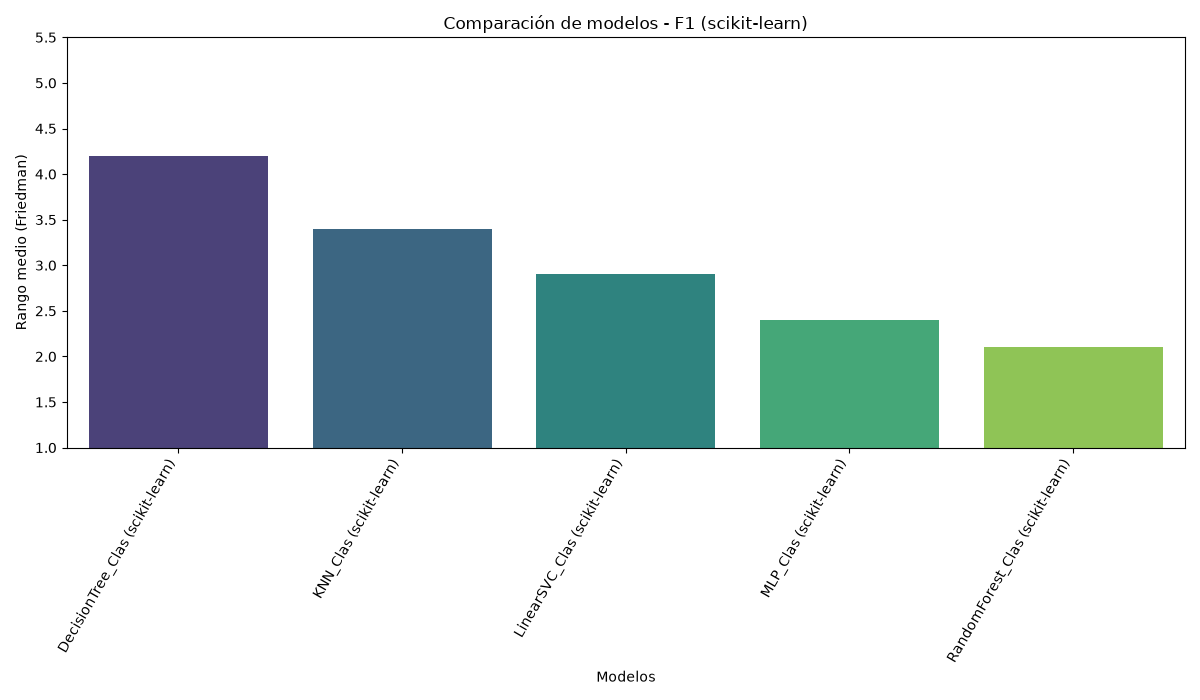
\includegraphics[width=1.0\textwidth]{sklearn_average_ranks_f1.png}
    \caption{Rangos medios de los modelos scikit-learn en clasificación según F1-score.}
    \label{fig:sklearn_ranks_f1}
\end{figure}
\begin{figure}[htbp]
    \centering
    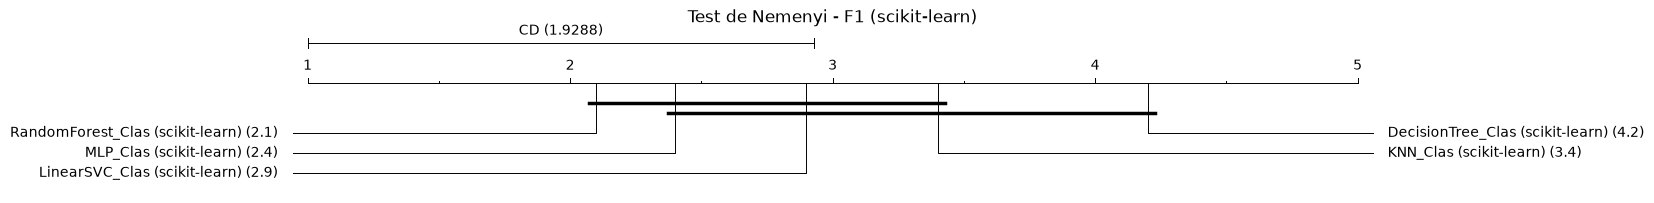
\includegraphics[width=1.0\textwidth]{sklearn_nemenyi_f1.png}
    \caption{Diagrama de distancia crítica de Nemenyi para los modelos scikit-learn en clasificación según F1-score.}
    \label{fig:sklearn_nemenyi_f1}
\end{figure}

El test de Friedman ($p\text{-valor} = 0.0252$) y el test de Iman-Davenport ($p\text{-valor} = 0.0170$) rechazan
fuertemente la hipótesis nula, confirmando que existen diferencias estadísticamente significativas en la capacidad
predictiva de los modelos.\\

En el primer gráfico se observa la clasificación de los rangos medios, donde un valor menor indica mejor posicionamiento.
El Random Forest (2.1) y el MLP (2.4) lideran la tabla, confirmando su superioridad generalizada. Decision Tree queda
relegado a la última posición con un rango de 4.2.\\

Para comprender qué diferencias son realmente significativas, recurrimos al test de Nemenyi. Con una distancia crítica
de 1.9288, el diagrama de Nemenyi conecta mediante líneas horizontales a los modelos cuyo rendimiento no difiere
estadísticamente. El hallazgo más notable aquí es que Random Forest supera significativamente a Decision Tree, ya que la
diferencia de sus rangos es mayor que la CD. Sin embargo, no existe una diferencia estadísticamente significativa entre
RF, MLP, LinearSVC e incluso k-NN bajo este nivel de confianza, lo que indica que, dependiendo de la naturaleza del
dataset, cualquiera de estos cuatro podría ofrecer resultados competitivos.

\newpage
\subsubsection{Huella de memoria (tamaño en disco en KB)}
\begin{table}[htbp]
  \centering
  \small % Reduce ligeramente el tamaño de la fuente para mejorar la legibilidad
  % 'l' para la primera columna de datasets y 'X' para que las de modelos se distribuyan equitativamente
  \begin{tabularx}{\textwidth}{l *{5}{>{\centering\arraybackslash}X}}
    \hline
    \textbf{Dataset} & \textbf{DT} & \textbf{k-NN} & \textbf{LinearSVC} & \textbf{MLP} & \textbf{RF} \\
    \hline
    CAR                & 14.74512  & 125.71777   & 2.12402  & 28.95996  & 610.75391  \\
    DIABETES           & 16.69043  & 73.74805    & 1.19141  & 23.32324  & 279.85449  \\
    GAMMA              & 59.81836  & 2118.52051  & 1.25391  & 23.55371  & 874.18457  \\
    HAR                & 30.57715  & 36188.59082 & 40.4834  & 603.55078 & 853.61426  \\
    IRIS               & 2.60840   & 9.41797     & 1.14844  & 20.50293  & 36.69336   \\
    LETTER RECOGNITION & 160.3584  & 1126.53125  & 4.85840  & 33.92578  & 3696.67871 \\
    MNIST              & 138.51758 & 24581.98926 & 80.66797 & 430.11328 & 2831.25293 \\
    SOYBEAN            & 25.46777  & 80.86328    & 7.17578  & 40.67188  & 543.35352  \\
    STUDENT DROPOUT    & 48.15820  & 527.23047   & 2.66016  & 37.41113  & 937.64160  \\
    WINE               & 2.26465   & 27.34277    & 1.57324  & 24.49023  & 38.24316   \\
    \hline
    \textbf{Media global} & \textbf{49.92061} & \textbf{6485.99521} & \textbf{14.31367} & \textbf{126.65029} & \textbf{1070.22705} \\
    \hline
  \end{tabularx}
  \caption{Tamaño en disco por dataset para los modelos scikit-learn base en clasificación.}
  \label{tab:sklearn_clas_size}
\end{table}

LinearSVC es, con notable diferencia, el modelo más ligero, presentando una media de tan solo 14.31 KB. Esto se debe
a que el modelo únicamente necesita almacenar los coeficientes del hiperplano separador y su sesgo,
independientemente del número de muestras de entrenamiento. De forma similar, el Decision Tree (DT) resulta altamente
eficiente en memoria con unos 49.92 KB de media, ya que su estructura se reduce a un conjunto finito de nodos y
umbrales de decisión.\\

En el extremo opuesto se encuentra k-NN, con un desorbitado tamaño medio de 6485.99 KB. Al ser un algoritmo de
aprendizaje vago, no construye un modelo generalizado, sino que se ve obligado a almacenar en memoria el conjunto de
entrenamiento al completo para poder calcular las distancias durante la inferencia. Esto se hace críticamente
evidente en conjuntos de datos voluminosos como \textbf{HAR} o \textbf{MNIST}, donde el modelo alcanza tamaños de
36.1 MB y 24.5 MB, respectivamente, cifras inasumibles para microcontroladores estándar.\\

Por su parte, Random Forest (RF) y MLP presentan pesos intermedios, coherentes con la necesidad de almacenar
múltiples árboles en el caso del primero, y diversas matrices de pesos para las capas ocultas en el caso del segundo.\\

\newpage
\begin{figure}[htbp]
    \centering
    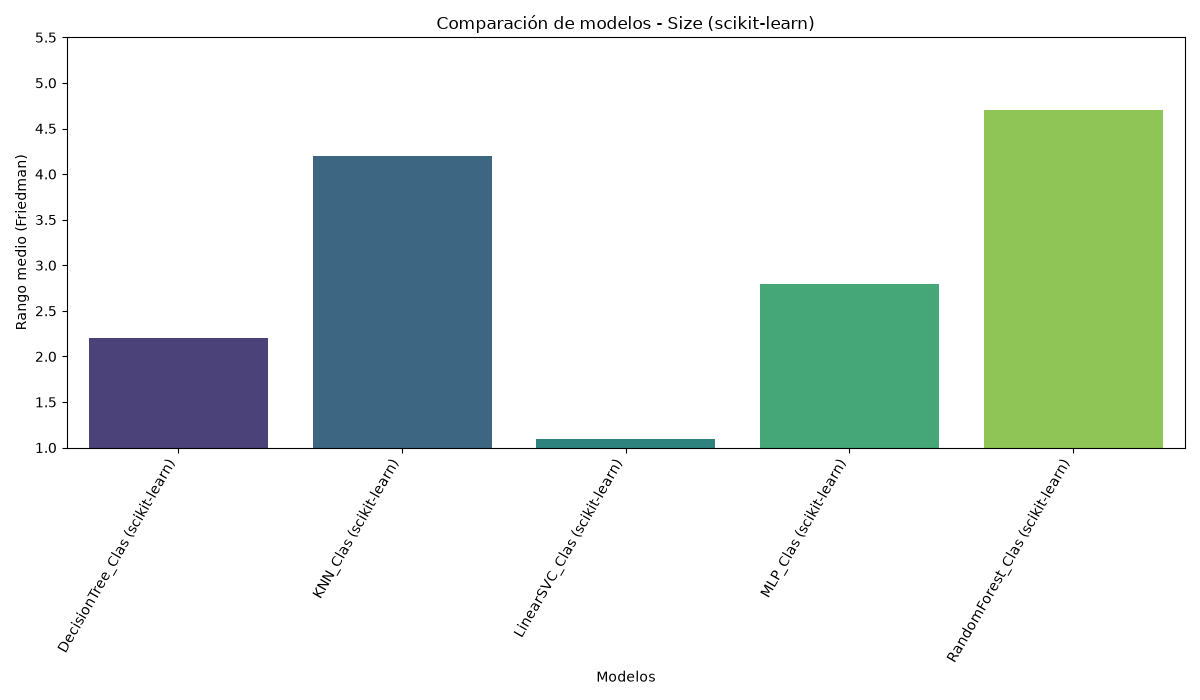
\includegraphics[width=1.0\textwidth]{sklearn_average_ranks_size.png}
    \caption{Rangos medios de los modelos scikit-learn en clasificación según el tamaño en disco.}
    \label{fig:sklearn_ranks_size}
\end{figure}
\begin{figure}[htbp]
    \centering
    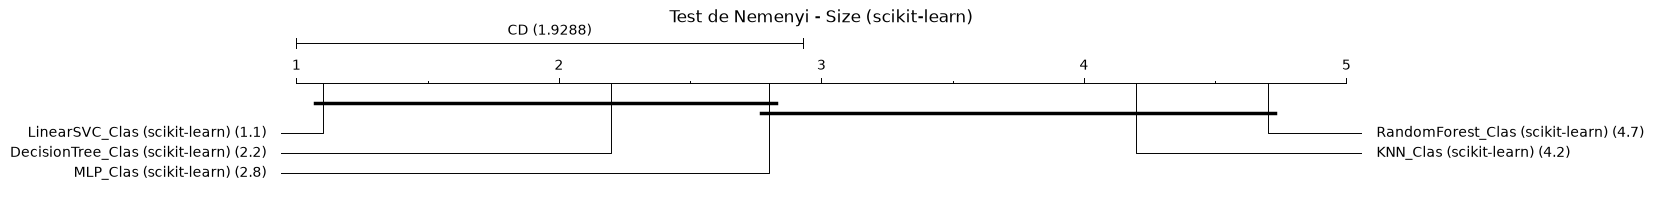
\includegraphics[width=1.0\textwidth]{sklearn_nemenyi_size.png}
    \caption{Diagrama de distancia crítica de Nemenyi para los modelos scikit-learn en clasificación según el tamaño en disco.}
    \label{fig:sklearn_nemenyi_size}
\end{figure}

Las pruebas estadísticas sobre el tamaño en disco ($p\text{-valor} \approx 0.0000$) rechazan de forma concluyente la
equivalencia entre arquitecturas.\\

Los rangos medios revela que LinearSVC domina esta métrica de forma casi absoluta con un rango medio de 1.1, muy seguido
por Decision Tree y MLP. En contraste, k-NN y Random Forest se posicionan como las alternativas más pesadas.\\

El gráfico de la distancia crítica de Nemenyi ilustra claramente la penalización estructural de los modelos basados en
memorización y ensamblado. La diferencia de rango entre LinearSVC y los modelos k-NN y Random Forest supera holgadamente
la distancia crítica. Esto valida estadísticamente la afirmación de que, para entornos con restricciones severas de
almacenamiento flash o RAM, algoritmos como k-NN, que almacena todo el conjunto de entrenamiento, o Random Forest, que
almacena decenas o cientos de árboles de decisión completos, quedan invalidados, siendo LinearSVC o Decision Tree, junto
al MLP las únicas opciones fiables y estadísticamente inferiores en coste.\\

\newpage
\subsubsection{Eficiencia operativa (ms) y resultados globales}
\begin{table}[htbp]
  \centering
  \small
  \begin{tabularx}{\textwidth}{l *{3}{>{\centering\arraybackslash}X}}
    \hline
    \textbf{Modelo} & \textbf{F1} & \textbf{Inferencia (ms)} & \textbf{Tamaño (KB)} \\
    \hline
    DecisionTree    & 0.82853 & 0.059  & 49.92061   \\
    KNeighbors      & 0.83775 & 1.162  & 6485.99521 \\
    LinearSVC       & 0.84554 & 0.18   & 14.31367   \\
    MLP             & 0.88738 & 0.231  & 126.65029  \\
    RandomForest    & 0.87371 & 14.001 & 1070.22705 \\
    \hline
  \end{tabularx}
  \caption{Resumen de eficiencia operativa y coste computacional de los modelos scikit-learn base en clasificación.}
  \label{tab:sklearn_clas_resumen}
\end{table}

El Decision Tree se consolida como el modelo más rápido durante la inferencia con 0.059 ms, ya que evaluar una nueva
muestra solo requiere atravesar una serie de saltos condicionales lógicos en memoria. Le sigue LinearSVC con 0.18 ms,
cuyo coste es el de unas simples multiplicaciones y sumas vectoriales.\\

El coste de los algoritmos más precisos resulta evidente en esta tabla. Random Forest, a pesar de su excelente F1,
es el algoritmo más lento debido a que cada inferencia requiere que la muestra atraviese todos los árboles del bosque
para realizar la votación final. Por otro lado, k-NN también penaliza fuertemente en tiempo, al exigir el cómputo de
la métrica de distancia de la nueva muestra contra miles de instancias guardadas en memoria.\\

Como conclusión parcial, si el objetivo es maximizar la exactitud sin restricciones de hardware, el MLP ofrece el
mejor balance general. Sin embargo, en un escenario de recursos fuertemente restringidos donde existan cuellos de
botella tanto de almacenamiento como energéticos, LinearSVC se postula como la arquitectura más eficiente, perdiendo
apenas un $\sim4.7\%$ de F1 respecto al MLP, pero reduciendo el tamaño en memoria en un factor de $\times 8.8$ y
superándolo en velocidad de inferencia.\\

\begin{figure}[htbp]
    \centering
    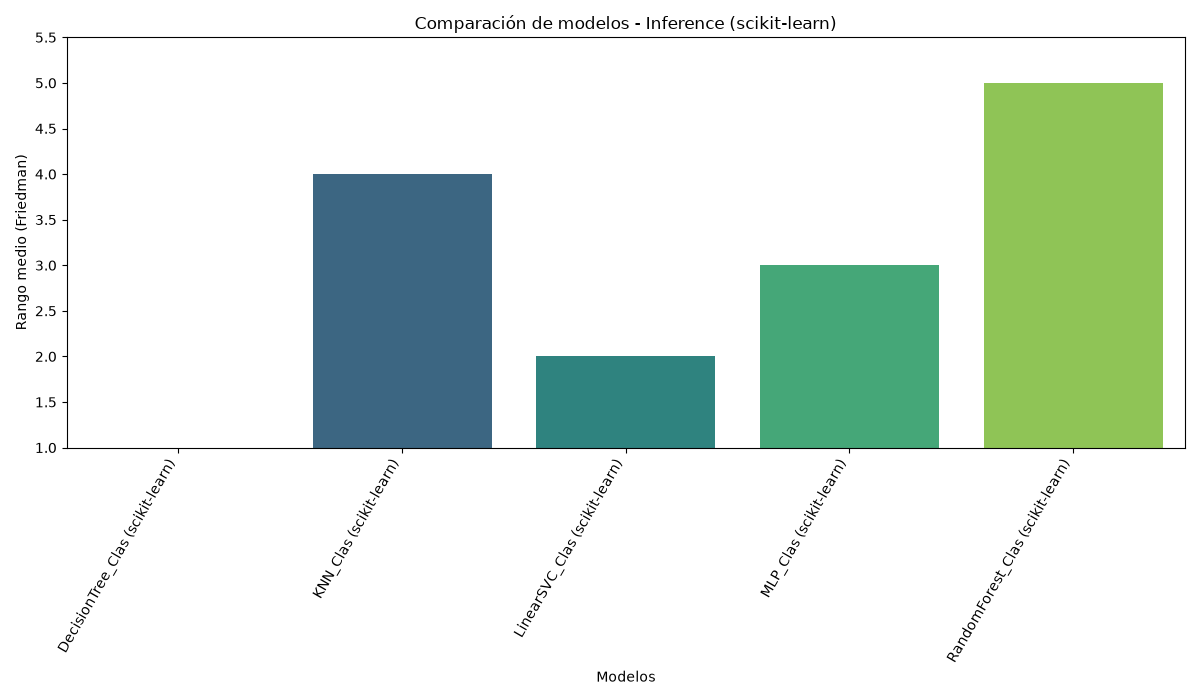
\includegraphics[width=0.82\textwidth]{sklearn_average_ranks_inference.png}
    \caption{Rangos medios de los modelos scikit-learn en clasificación según el tiempo de inferencia.}
    \label{fig:sklearn_ranks_inference}
\end{figure}
\newpage
\begin{figure}[htbp]
    \centering
    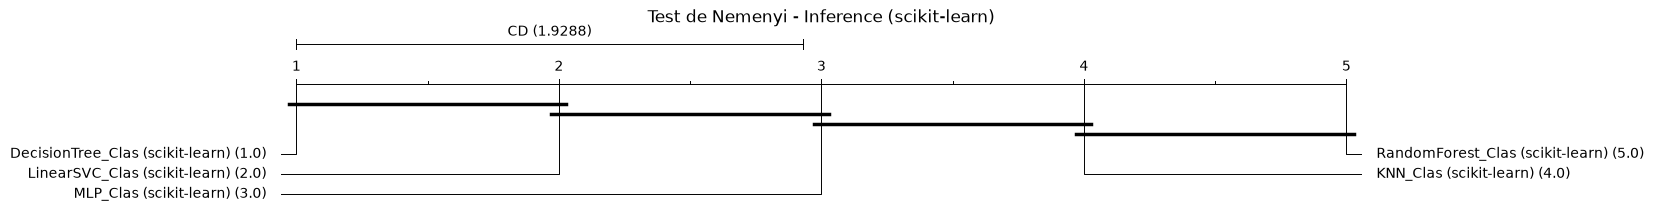
\includegraphics[width=1.0\textwidth]{sklearn_nemenyi_inference.png}
    \caption{Diagrama de distancia crítica de Nemenyi para los modelos scikit-learn en clasificación según el tiempo de inferencia.}
    \label{fig:sklearn_nemenyi_inference}
\end{figure}

El análisis de los tiempos de inferencia arroja resultados contundentes. Tanto el test de Friedman como el de
Iman-Davenport devuelven un $p\text{-valor} \approx 0.0000$, evidenciando una separación drástica en la eficiencia
computacional de los algoritmos.\\

El gráfico de rangos medios dibuja una escalera perfecta que refleja la complejidad asintótica de cada método. Decision
Tree obtiene un rango ideal de 1.0, seguido de LinearSVC, MLP, k-NN y Random Forest.\\

Al analizar el gráfico de distancia crítica, observamos múltiples aislamientos estadísticos. Decision Tree es
significativamente más rápido que MLP, k-NN y Random Forest. Por su parte, los modelos paramétricos ligeros (LinearSVC y
MLP) se agrupan demostrando que las operaciones matriciales precalculadas son mucho más eficientes que los algoritmos de
evaluación perezosa (k-NN) o los métodos de ensamblado masivo (Random Forest). Queda estadísticamente probado que el
coste temporal de Random Forest es significativamente superior al de las opciones lineales y basadas en árboles simples.

\subsubsection{Regresión}
Tras evaluar el comportamiento de los modelos de scikit-learn en clasificación, esta sección replica la metodología para
la tarea de regresión. Se evalúan cinco arquitecturas clásicas: Decision Tree (DT), k-NN, regresión lineal (LinearReg),
perceptrón multicapa (MLP) y Random Forest (RF), empleando como métrica de rendimiento el coeficiente de determinación
(R$^2$), junto con los tiempos de inferencia y la huella de memoria.

\subsubsection{Rendimiento predictivo (R$^2$)}
\begin{table}[htbp]
  \centering
  \small
  \begin{tabularx}{\textwidth}{l *{5}{>{\centering\arraybackslash}X}}
    \hline
    \textbf{Dataset} & \textbf{DT} & \textbf{k-NN} & \textbf{LinReg} & \textbf{MLP} & \textbf{RF} \\
    \hline
    ABALONE                      & 0.31095 & 0.48702 & 0.52797 & 0.56687 & 0.54030 \\
    AIR QUALITY                  & 0.83286 & 0.84806 & 0.85493 & 0.87918 & 0.88917 \\
    APPLIANCES ENERGY PREDICTION & 0.64248 & 0.61135 & 0.62108 & 0.68788 & 0.69304 \\
    AUTOMOBILE                   & 0.84311 & 0.78158 & 0.84668 & 0.86248 & 0.90958 \\
    BIKE SHARING HOURLY          & 0.89224 & 0.67717 & 0.38781 & 0.92571 & 0.76308 \\
    COMMUNITIES AND CRIME        & 0.30799 & 0.59557 & 0.65104 & 0.55782 & 0.64034 \\
    OBESITY LEVELS               & 0.98418 & 0.88298 & 0.56080 & 0.97471 & 0.96036 \\
    REAL ESTATE VALUATION        & 0.49584 & 0.60493 & 0.57181 & 0.65777 & 0.71083 \\
    STUDENT PERFORMANCE          & 0.76874 & 0.31862 & 0.79571 & 0.65802 & 0.71844 \\
    WINE QUALITY                 & 0.21155 & 0.47764 & 0.27424 & 0.33979 & 0.44201 \\
    \hline
    \textbf{Media global} & \textbf{0.62899} & \textbf{0.62849} & \textbf{0.60921} & \textbf{0.71102} & \textbf{0.72671} \\
    \hline
  \end{tabularx}
  \caption{R$^2$ por dataset para los modelos scikit-learn base en regresión.}
  \label{tab:sklearn_r2}
\end{table}

A diferencia de la clasificación, donde las métricas de acierto puro suelen ser más optimistas, el coeficiente R$^2$
penaliza severamente las desviaciones absolutas, revelando con mayor crudeza los límites de los modelos de aprendizaje
automático clásico para modelar variables continuas.\\

A nivel global, Random Forest y MLP destacan como las arquitecturas más robustas y precisas, logrando medias de 0.72671 y
0.71102, respectivamente. Esta superioridad radica en la capacidad de ambos algoritmos para capturar complejas relaciones
no lineales e interacciones multivariantes. Resulta paradigmático el comportamiento en datasets como
\textbf{BIKE SHARING HOURLY}, donde la regresión lineal colapsa (0.38781), mientras que MLP (0.92571) y DT (0.89224)
logran excelentes resultados. Esto sugiere una fuerte presencia de características no lineales y estacionales que los
modelos lineales estándar son incapaces de aproximar sin un complejo trabajo de ingeniería de características.\\

Los algoritmos más simples (DT, k-NN y LinearReg) conforman un bloque inferior con un rendimiento global empatado en
torno a 0.60-0.62. Sin embargo, su desempeño fluctúa enormemente dependiendo del dominio. Por ejemplo, en el dataset
\textbf{OBESITY LEVELS}, DT obtiene un excelente 0.98418 (sugiriendo la presencia de límites de decisión ortogonales muy
claros en los datos), mientras que en \textbf{WINE QUALITY} sufre un severo sobreajuste o incapacidad de
generalización (0.21155). Por su parte, la regresión lineal muestra una clara deficiencia global (0.60921), actuando
como límite inferior esperado cuando la topología del problema carece de linealidad directa entre los descriptores y la
variable objetivo.\\

\begin{figure}[htbp]
    \centering
    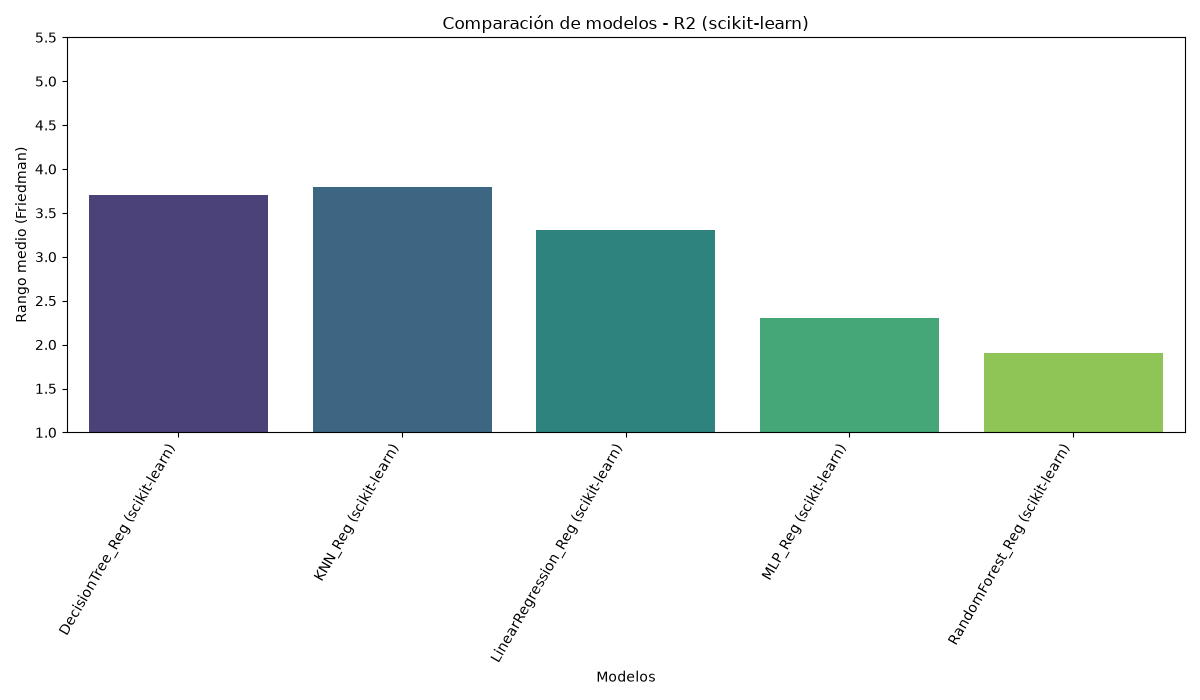
\includegraphics[width=1.0\textwidth]{sklearn_reg_average_ranks_r2.png}
    \caption{Rangos medios de los modelos scikit-learn en regresión según R$^2$.}
    \label{fig:sklearn_ranks_r2}
\end{figure}
\begin{figure}[htbp]
    \centering
    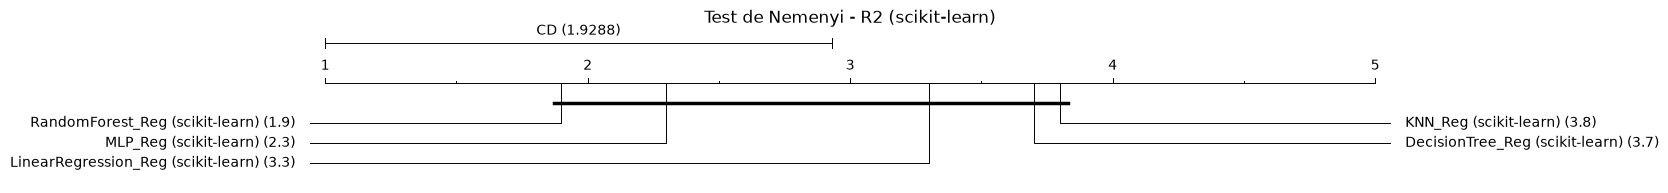
\includegraphics[width=1.0\textwidth]{sklearn_reg_nemenyi_r2.png}
    \caption{Diagrama de distancia crítica de Nemenyi para los modelos scikit-learn en regresión según R$^2$.}
    \label{fig:sklearn_nemenyi_r2}
\end{figure}

Los tests de Friedman ($p\text{-valor} = 0.0198$) y de Iman-Davenport ($p\text{-valor} = 0.0125$) confirman que el
rendimiento de los modelos no es equivalente.\\

Los rangos medios muestra que el random forest (1.9) y el MLP (2.3) se posicionan como las arquitecturas con mejor
capacidad de generalización general, mientras que k-NN y Decision Tree ocupan los últimos lugares.\\

Sin embargo, el test de Nemenyi revela un fenómeno estadístico interesante. El test revela que la diferencia entre el
mejor modelo (Random Forest, 1.9) y el peor (k-NN, 3.8) es exactamente 1.9, rozando el umbral de la distancia crítica
(1.9288). Esto indica que, si bien la tendencia favorece claramente a los ensamblados y redes neuronales, la variabilidad
del rendimiento según el dataset en regresión es tan acusada que no se puede afirmar con un 95\% de confianza que una
arquitectura simple vaya a ser siempre inferior a una compleja para cualquier problema tabular arbitrario.

\subsubsection{Huella de memoria (tamaño en disco en KB)}
\begin{table}[htbp]
  \centering
  \small
  \begin{tabularx}{\textwidth}{l *{5}{>{\centering\arraybackslash}X}}
    \hline
    \textbf{Dataset} & \textbf{DT} & \textbf{k-NN} & \textbf{LinReg} & \textbf{MLP} & \textbf{RF} \\
    \hline
    ABALONE                      & 69.03223  & 456.23047  & 1.16602 & 22.72266 & 1171.95801 \\
    AIR QUALITY                  & 95.18848  & 1580.02246 & 2.51855 & 44.53223 & 1775.45020 \\
    APPLIANCES ENERGY PREDICTION & 82.81348  & 2159.87012 & 1.92480 & 34.82812 & 1415.30957 \\
    AUTOMOBILE                   & 17.55176  & 49.56543   & 3.18066 & 64.53516 & 232.02148  \\
    BIKE SHARING HOURLY          & 125.98535 & 2231.62598 & 1.22852 & 25.17773 & 2195.91895 \\
    COMMUNITIES AND CRIME        & 54.96094  & 632.58887  & 3.99316 & 69.17773 & 923.17480  \\
    OBESITY LEVELS               & 13.89551  & 186.21680  & 1.69727 & 31.43555 & 505.90527  \\
    REAL ESTATE VALUATION        & 27.67969  & 30.65625   & 1.04102 & 21.96289 & 433.48340  \\
    STUDENT PERFORMANCE          & 18.25488  & 75.15527   & 2.67480 & 48.24414 & 347.50879  \\
    WINE QUALITY                 & 47.22656  & 604.54004  & 1.19727 & 23.04004 & 830.22168  \\
    \hline
    \textbf{Media global} & \textbf{55.25889} & \textbf{800.64717} & \textbf{2.06221} & \textbf{38.56562} & \textbf{983.09521} \\
    \hline
  \end{tabularx}
  \caption{Tamaño en disco (KB) por dataset para los modelos scikit-learn base en regresión.}
  \label{tab:sklearn_reg_size}
\end{table}

Si evaluamos la eficiencia en términos de almacenamiento, el análisis físico de los modelos guarda un paralelismo directo
con lo observado en los problemas de clasificación, exponiendo la naturaleza subyacente de cada algoritmo.\\

La regresión lineal es el algoritmo más eficiente del ecosistema evaluado, con un tamaño residual medio de apenas 2.06 KB.
Matemáticamente, el modelo solo necesita persistir un vector de coeficientes $\beta$ (de longitud igual al número de
variables predictoras) y un término independiente. De igual modo, el MLP (38.56 KB) y el Decision Tree (55.25 KB)
demuestran ser arquitecturas altamente eficientes, persistiendo únicamente matrices de pesos interconectadas o reglas de
ramificación condicional, respectivamente.\\

En el extremo opuesto, los algoritmos basados en la retención de datos y ensamblados densos vuelven a penalizar
drásticamente la huella de memoria. El Random Forest escala hasta los 983.09 KB debido al almacenamiento de la estructura
completa del ensamble arbóreo. Por otro lado, k-NN vuelve a evidenciar su limitación como modelo \textit{lazy},
alcanzando los 800.64 KB de media, pero disparándose hasta los 2.2 MB en conjuntos de alta densidad como
\textbf{BIKE SHARING HOURLY} o \textbf{APPLIANCES ENERGY PREDICTION}, lo que limita severamente su viabilidad en sistemas
embebidos.\\

\begin{figure}[htbp]
    \centering
    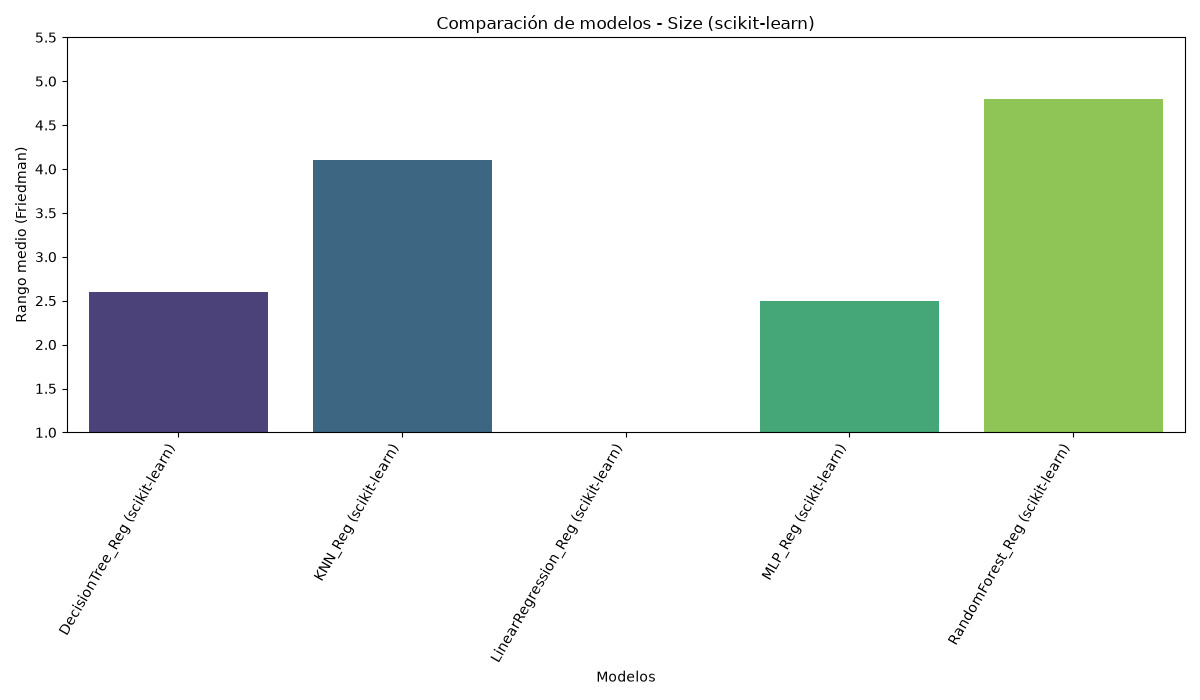
\includegraphics[width=1.0\textwidth]{sklearn_reg_average_ranks_size.png}
    \caption{Rangos medios de los modelos scikit-learn en regresión según el tamaño en disco.}
    \label{fig:sklearn_reg_ranks_size}
\end{figure}
\begin{figure}[htbp]
    \centering
    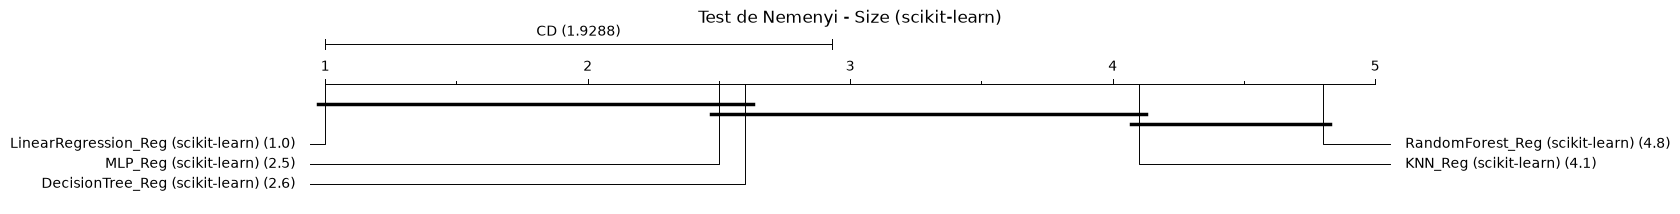
\includegraphics[width=1.0\textwidth]{sklearn_reg_nemenyi_size.png}
    \caption{Diagrama de distancia crítica de Nemenyi para los modelos scikit-learn en regresión según el tamaño en disco.}
    \label{fig:sklearn_reg_nemenyi_size}
\end{figure}

Las pruebas sobre el almacenamiento en disco arrojan diferencias estructurales insalvables ($p\text{-valor} 
\approx 0.0000$ en Friedman e Iman-Davenport).\\

Los rangos medios sitúan a la regresión lineal en el rango absoluto de la perfección (1.0), confirmando que en todos los
datasets generó el archivo más ligero. MLP (2.5) y Decision Tree (2.6) conforman la clase media, mientras que k-NN y
Random Forest son los más ineficientes.\\

A través de la distancia crítica de Nemenyi, las conclusiones cualitativas previas quedan selladas. La regresión lineal es
estadísticamente más ligera que k-NN y Random Forest. De igual manera, MLP y Decision Tree también logran separarse
significativamente de Random Forest, demostrando que la memorización estructural de conjuntos de árboles es el enfoque
menos viable para un despliegue bajo estrictas restricciones de hardware.

\subsubsection{Eficiencia operativa (ms) y resultados globales}
\begin{table}[htbp]
  \centering
  \small
  \begin{tabularx}{\textwidth}{l *{3}{>{\centering\arraybackslash}X}}
    \hline
    \textbf{Modelo} & \textbf{R$^2$} & \textbf{Inferencia (ms)} & \textbf{Tamaño (KB)} \\
    \hline
    DecisionTree    & 0.62899 & 0.055  & 55.25889  \\
    KNeighbors      & 0.62849 & 0.673  & 800.64717 \\
    LinearReg       & 0.60921 & 0.153  & 2.06221   \\
    MLP             & 0.71102 & 0.157  & 38.56562  \\
    RandomForest    & 0.72671 & 14.014 & 983.09521 \\
    \hline
  \end{tabularx}
  \caption{Resumen de eficiencia operativa y coste computacional de los modelos scikit-learn base en regresión.}
  \label{tab:sklearn_reg_resumen}
\end{table}

El Decision Tree repite como la arquitectura más rápida en inferencia, con 0.055 ms, siendo el modelo óptimo si la
latencia es un factor de vida o muerte para el sistema, aunque a expensas de sacrificar estabilidad predictiva frente al
sobreajuste.\\

La regresión lineal y el MLP se posicionan en un interesante rango intermedio de eficiencia ($\sim$ 0.15 ms). Es de
especial relevancia el comportamiento del MLP: a pesar de presentar un tiempo de latencia en inferencia idéntico en
magnitud al de la regresión lineal, logra aumentar el R$^2$ medio en más de un 16\% (de 0.609 a 0.711). Esto consolida
al perceptrón multicapa como el algoritmo con mejor equilibrio entre exactitud y eficiencia temporal para regresión
tabular en scikit-learn.\\

Por último, el Random Forest vuelve a poner de manifiesto el coste del aprendizaje en grupo. Si bien logra el mejor poder
predictivo general, el proceso computacional de atravesar y promediar las salidas de múltiples árboles individuales eleva
su tiempo de inferencia hasta los $14.0$ ms. Esto representa un retardo casi 100 veces mayor que el MLP o la regresión
lineal, un coste latente inasumible para sistemas que requieran procesamiento en tiempo real estricto.\\

\newpage
\begin{figure}[htbp]
    \centering
    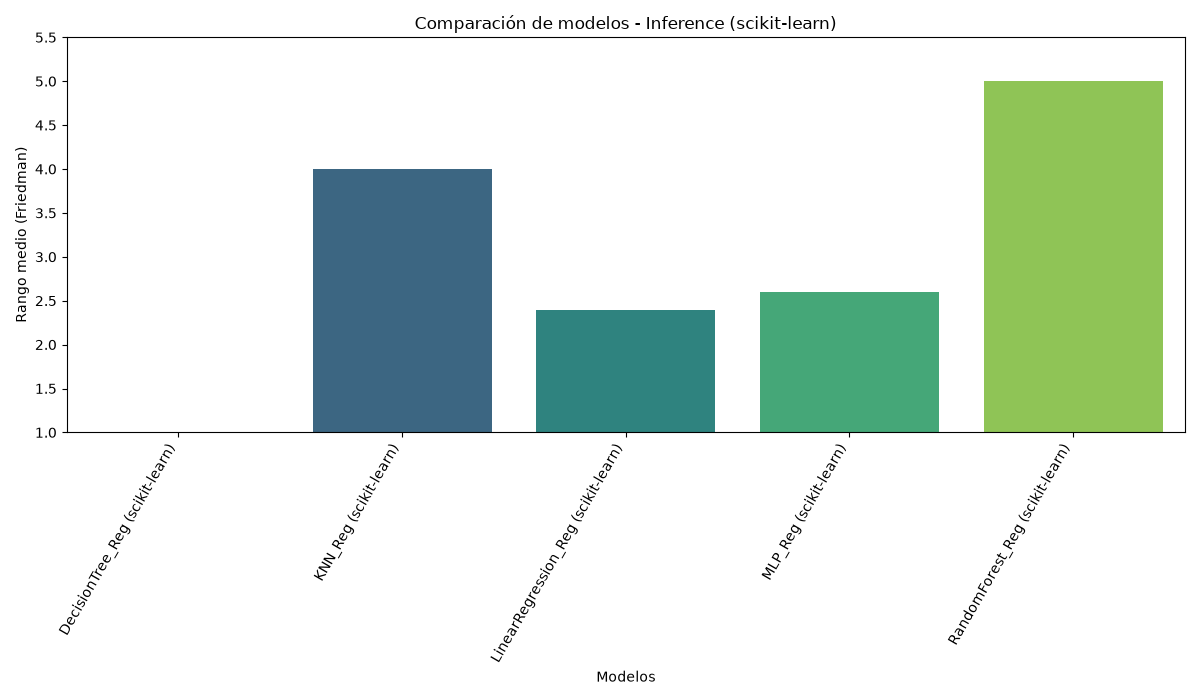
\includegraphics[width=1.0\textwidth]{sklearn_reg_average_ranks_inference.png}
    \caption{Rangos medios de los modelos scikit-learn en regresión según el tiempo de inferencia.}
    \label{fig:sklearn_reg_ranks_inference}
\end{figure}
\begin{figure}[htbp]
    \centering
    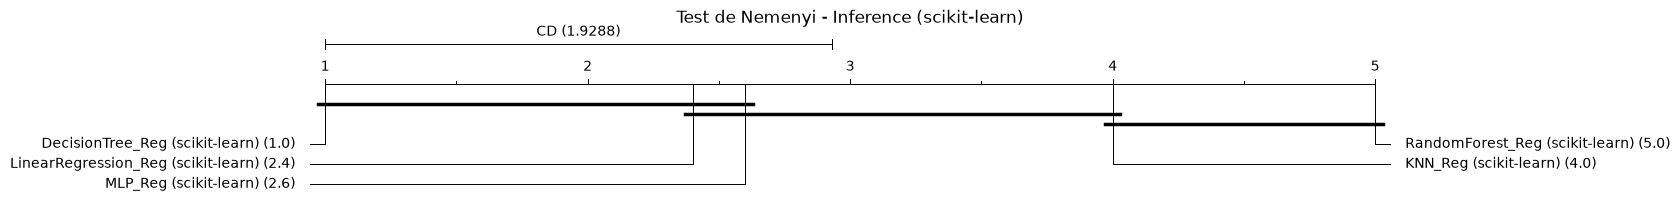
\includegraphics[width=1.0\textwidth]{sklearn_reg_nemenyi_inference.png}
    \caption{Diagrama de distancia crítica de Nemenyi para los modelos scikit-learn en regresión según el tiempo de inferencia.}
    \label{fig:sklearn_reg_nemenyi_inference}
\end{figure}

Las pruebas sobre el almacenamiento en disco muestran un resultado igualmente concluyente ($p\text{-valor} \approx 0.0000$).\\

Los rangos de Friedman establecen una jerarquía clara: Decision Tree (1.0) es unánimemente el modelo más rápido, seguido
de un empate virtual entre LinearRegression (2.4) y MLP (2.6). Random Forest queda en última posición.\\

El test de Nemenyi confirma tres grupos bien diferenciados. Primero, Decision Tree es significativamente más veloz que
k-NN y Random Forest. Segundo, los modelos matemáticos de inferencia paramétrica directa (LinearRegression y MLP) no
difieren estadísticamente del Decision Tree, pero sí son significativamente más rápidos que el pesado proceso iterativo de
Random Forest. Esto demuestra matemáticamente, como hasta ahora, que la alta precisión de Random Forest conlleva una
penalización temporal estadísticamente insalvable.

\subsection{ONNX}
\subsubsection{Clasificación}
En este bloque se analiza el impacto de exportar los modelos base de scikit-learn al formato ONNX y someterlos a un
proceso de cuantización, junto a las técnicas aplicadas a cada modelo de forma individual. El objetivo de esta fase es
evaluar si el uso de un motor de inferencia altamente optimizado para C++ como es ONNX y la reducción de la precisión
numérica logran mitigar los cuellos de botella detectados en scikit-learn, y a qué coste predictivo.

\subsubsection{Rendimiento predictivo (F1-score)}
\begin{table}[htbp]
  \centering
  \small
  \begin{tabularx}{\textwidth}{l *{5}{>{\centering\arraybackslash}X}}
    \hline
    \textbf{Dataset} & \textbf{DT} & \textbf{k-NN} & \textbf{LinearSVC} & \textbf{MLP} & \textbf{RF} \\
    \hline
    CAR                  & 0.91133 & 0.24862 & 0.84995 & 0.99783 & 0.79830 \\
    DIABETES             & 0.66107 & 0.57212 & 0.73463 & 0.65741 & 0.50480 \\
    GAMMA                & 0.28385 & 0.75875 & 0.76935 & 0.74975 & 0.26167 \\
    HAR                  & 0.93683 & 0.89033 & 0.98474 & 0.55758 & 0.92793 \\
    IRIS                 & 0.94869 & 0.73696 & 0.93578 & 0.95129 & 0.94856 \\
    LETTER RECOGNITION   & 0.72497 & 0.03079 & 0.69261 & 0.88530 & 0.62232 \\
    MNIST                & 0.80245 & 0.47632 & 0.85396 & 0.88022 & 0.75324 \\
    SOYBEAN              & 0.91378 & 0.64960 & 0.95943 & 0.90922 & 0.90764 \\
    STUDENT DROPOUT      & 0.64624 & 0.60265 & 0.69164 & 0.63269 & 0.66253 \\
    WINE                 & 0.90380 & 0.95275 & 0.98328 & 0.97251 & 0.89902 \\
    \hline
    \textbf{Media global} & \textbf{0.77330} & \textbf{0.59189} & \textbf{0.84554} & \textbf{0.81938} & \textbf{0.72860} \\
    \hline
  \end{tabularx}
  \caption{F1-score por dataset para los modelos ONNX $+$ cuantización en clasificación.}
  \label{tab:onnx_est_f1}
\end{table}
En este escenario, LinearSVC (0.84554) y MLP (0.81938) se alzan como las arquitecturas más estables y robustas. El éxito
de LinearSVC demuestra que forzar la dispersión de la matriz de pesos combinada con la cuantización no desplaza de forma
crítica los hiperplanos de decisión. De igual modo, el MLP soporta la poda de conexiones débiles reteniendo un alto poder
de generalización.\\

Por otro lado, la tendencia de rendimiento cambia para los modelos basados en particiones espaciales o ensamblados. El
modelo k-NN registra el rendimiento más pobre del estudio. Este resultado se explica por la agresiva reducción de
prototipos aplicada: al agrupar el espacio de características mediante \path{MiniBatchKMeans} y conservar un máximo de
200 centroides por clase, se destruye la resolución geométrica local, un efecto que se agrava fatalmente al cuantizar
dichas coordenadas a enteros de 8 bits.\\

Llama la atención el comportamiento de Random Forest, cuyo desempeño se asemeja sospechosamente al de un árbol simple. La
justificación radica en el proceso de destilación de conocimiento aplicado, mediante el cual el comportamiento del bosque
complejo ha sido transferido a un único árbol estudiante. Por tanto, su F1 no es el de un ensamble, sino el de un árbol
poco profundo intentando aproximar las decisiones del bosque original.\\

\newpage
\begin{figure}[htbp]
    \centering
    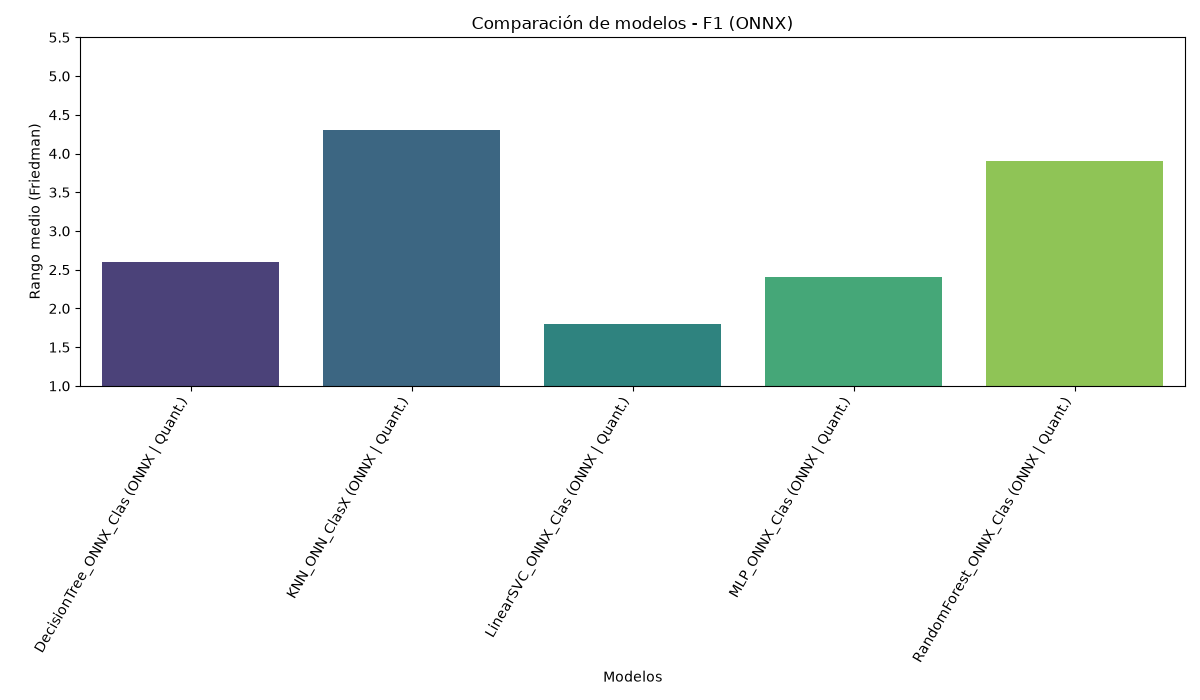
\includegraphics[width=1.0\textwidth]{onnx_average_ranks_f1.png}
    \caption{Rangos medios de los modelos ONNX en clasificación según F1-score.}
    \label{fig:onnx_ranks_f1}
\end{figure}
\begin{figure}[htbp]
    \centering
    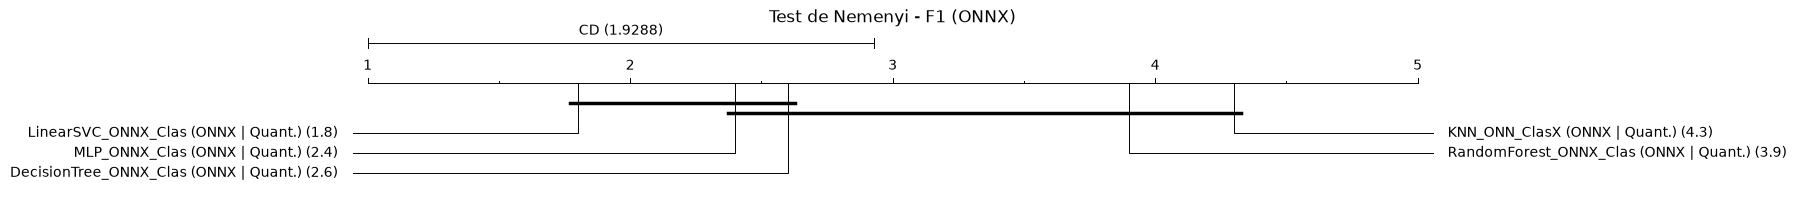
\includegraphics[width=1.0\textwidth]{onnx_nemenyi_f1.png}
    \caption{Diagrama de distancia crítica de Nemenyi para los modelos ONNX en clasificación según F1-score.}
    \label{fig:onnx_nemenyi_f1}
\end{figure}

Los tests globales ($p\text{-valor} = 0.0013$) confirman alteraciones significativas en la capacidad de acierto. LinearSVC
(1.8) y MLP (2.4) dominan la clasificación, mientras que Random Forest y k-NN caen a las últimas posiciones.\\

El diagrama de la distancia crítica valida matemáticamente el coste de la compresión: LinearSVC es estadísticamente
superior a Random Forest y k-NN. La diferencia de rangos supera la distancia crítica. Esto demuestra de forma concluyente
que la reducción de prototipos y la destilación, combinadas con cuantización, introducen una penalización predictiva
insalvable frente a la robustez geométrica de un hiperplano.

\subsubsection{Huella de memoria (tamaño en disco en KB)}
El impacto de las técnicas de compresión y la serialización a ONNX obtiene huellas de almacenamiento extremadamente
eficientes para la mayoría de arquitecturas.
\newpage
\begin{table}[htbp]
  \centering
  \small
  \begin{tabularx}{\textwidth}{l *{5}{>{\centering\arraybackslash}X}}
    \hline
    \textbf{Dataset} & \textbf{DT} & \textbf{k-NN} & \textbf{LinearSVC} & \textbf{MLP} & \textbf{RF} \\
    \hline
    CAR                  & 8.41211   & 16.84375   & 1.08203  & 8.80762  & 4.50195  \\
    DIABETES             & 8.07129   & 7.53516    & 0.60059  & 9.33691  & 5.33008  \\
    GAMMA                & 29.09766  & 22.60840   & 0.63965  & 9.41895  & 5.33008  \\
    HAR                  & 18.44434  & 915.1875   & 22.40039 & 31.00293 & 8.81543  \\
    IRIS                 & 1.59570   & 8.65918    & 0.55566  & 8.08887  & 1.59570  \\
    LETTER RECOGNITION   & 109.78223 & 96.81934   & 2.80566  & 9.03418  & 22.61426 \\
    MNIST                & 89.25098  & 1240.45605 & 46.45117 & 40.22852 & 11.60938 \\
    SOYBEAN              & 16.18457  & 60.79980   & 4.16016  & 9.67871  & 13.00781 \\
    STUDENT DROPOUT      & 27.62988  & 33.27148   & 1.34082  & 9.40430  & 6.70898  \\
    WINE                 & 1.40918   & 9.81055    & 0.77734  & 8.45898  & 1.40918  \\
    \hline
    \textbf{Media global} & \textbf{30.98779} & \textbf{241.19912} & \textbf{8.08135} & \textbf{14.34600} & \textbf{8.09229} \\
    \hline
  \end{tabularx}
  \caption{Tamaño en disco (KB) por dataset para los modelos ONNX $+$ cuantización en clasificación.}
  \label{tab:onnx_est_clas_size}
\end{table}

Los modelos paramétricos como LinearSVC (8.08 KB) y MLP (14.34 KB) alcanzan niveles de compresión idóneos para la
computación en el borde, favorecidos tanto por las reducciones implementadas.\\

El caso más extremo es el de Random Forest, cuyo tamaño promedio se sitúa en unos asombrosos 8.09 KB, siendo en varios
datasets incluso más ligero que el Decision Tree estándar (30.98 KB). Esta drástica minimización certifica el impacto
estructural de la destilación: en el almacenamiento físico ya no existe un bosque, sino el grafo serializado de un único
árbol estudiante muy acotado. Finalmente, aunque k-NN sigue siendo la arquitectura más pesada (241.19 KB), la
técnica de reducción de prototipos evita que la huella de memoria escale linealmente con el volumen de datos de los
datasets más masivos.

\begin{figure}[htbp]
    \centering
    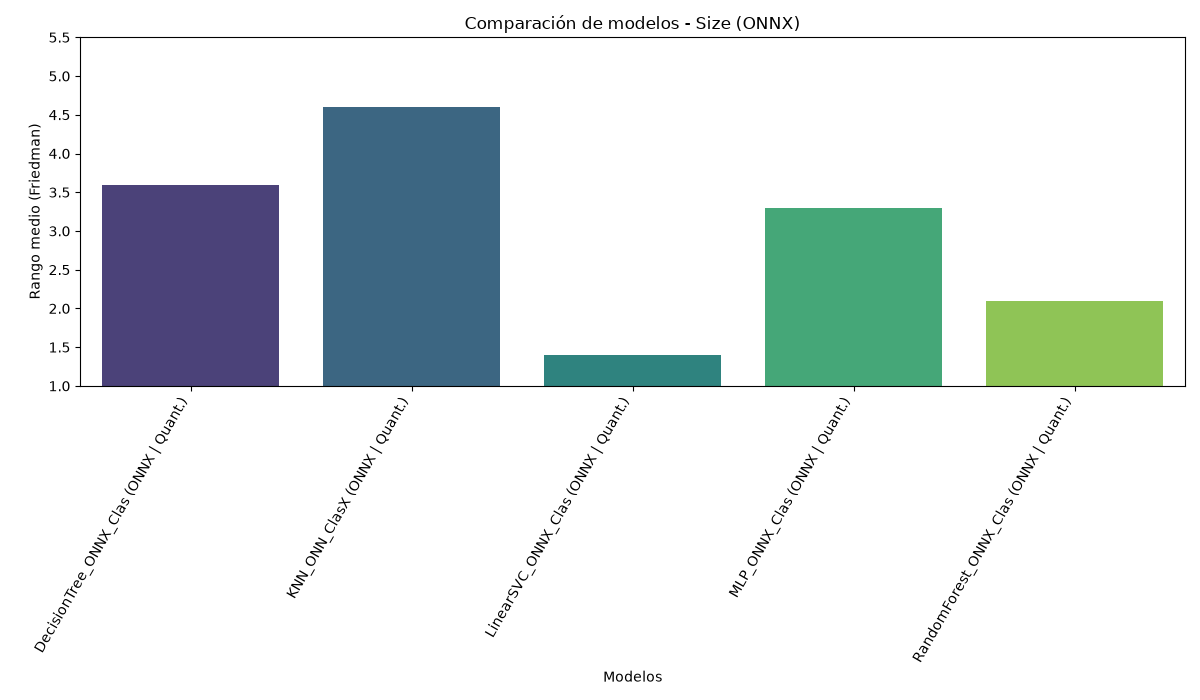
\includegraphics[width=1.0\textwidth]{onnx_average_ranks_size.png}
    \caption{Rangos medios de los modelos ONNX en clasificación según el tamaño en disco.}
    \label{fig:onnx_ranks_size}
\end{figure}
Las diferencias de compresión espacial son drásticas ($p\text{-valor} \approx 0.0000$). Los rangos medios confirman el
comportamiento de los modelos: LinearSVC (1.4) y el árbol estudiante destilado del Random Forest (2.1) lideran la
eficiencia.\\

\begin{figure}[htbp]
    \centering
    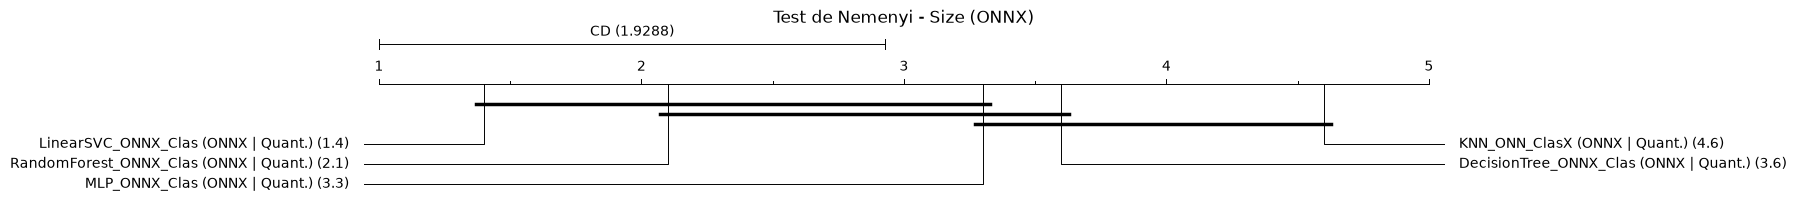
\includegraphics[width=1.0\textwidth]{onnx_nemenyi_size.png}
    \caption{Diagrama de distancia crítica de Nemenyi para los modelos ONNX en clasificación según el tamaño en disco.}
    \label{fig:onnx_nemenyi_size}
\end{figure}
Al observar la distancia crítica de Nemenyi, ambos modelos se aíslan significativamente del k-NN (4.6) y del Decision
Tree original (3.6). Queda probado que la destilación transforma un ensamble masivo en una estructura que es
estadísticamente más ligera que un árbol de decisión estándar sin podar.

\subsubsection{Eficiencia operativa (ms) y resultados globales}
\begin{table}[htbp]
  \centering
  \small
  \begin{tabularx}{\textwidth}{l *{3}{>{\centering\arraybackslash}X}}
    \hline
    \textbf{Modelo} & \textbf{F1} & \textbf{Inferencia (ms)} & \textbf{Tamaño (KB)} \\
    \hline
    DecisionTree    & 0.77330 & 0.01  & 30.98779  \\
    KNeighbors      & 0.59189 & 0.515 & 241.19912 \\
    LinearSVC       & 0.84554 & 0.01  & 8.08135   \\
    MLP             & 0.81938 & 0.023 & 14.34600  \\
    RandomForest    & 0.72860 & 0.01  & 8.09229   \\
    \hline
  \end{tabularx}
  \caption{Resumen de eficiencia operativa y coste computacional de los modelos ONNX $+$ cuantización en clasificación .}
  \label{tab:onnx_est_clas_resumen}
\end{table}
Las arquitecturas lógicas y lineales convergen de manera unánime en el límite de latencia inferior medible para este
entorno: 0.01 ms. Nuevamente, la extrema velocidad del Random Forest evidencia su transformación topológica. Al haber
sido destilado en un árbol estudiante de profundidad máxima 8, la inferencia se reduce a un máximo de 8 saltos
condicionales en memoria, erradicando el cuello de botella computacional del ensamblado masivo.\\

El MLP muestra una latencia algo superior (0.023 ms), coherente con la necesidad de ejecutar sumas y multiplicaciones
matriciales en las capas ocultas, aunque fuertemente aceleradas por la cuantización. k-NN, con 0.515 ms ocupa la última
posición, de modo que iterar computando distancias contra los centroides retenidos sigue siendo la operación más costosa
del espectro, incluso en C++.

\newpage
\begin{figure}[htbp]
    \centering
    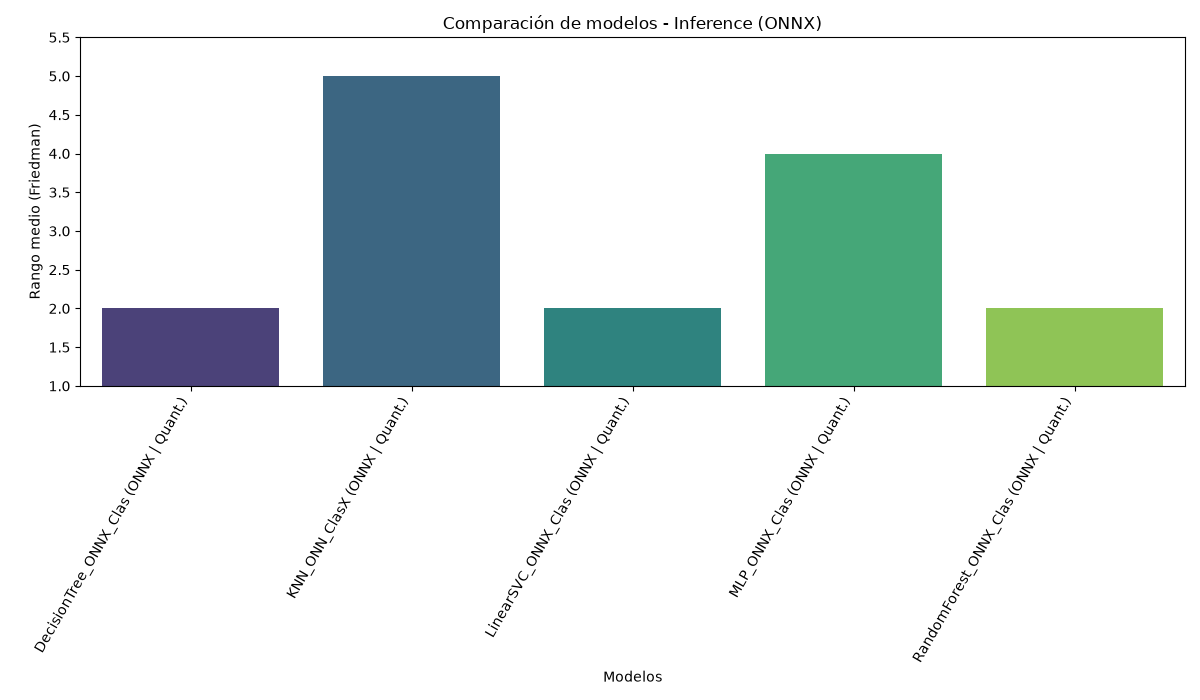
\includegraphics[width=1.0\textwidth]{onnx_average_ranks_inference.png}
    \caption{Rangos medios de los modelos ONNX en clasificación según el tiempo de inferencia.}
    \label{fig:onnx_ranks_inference}
\end{figure}
\begin{figure}[htbp]
    \centering
    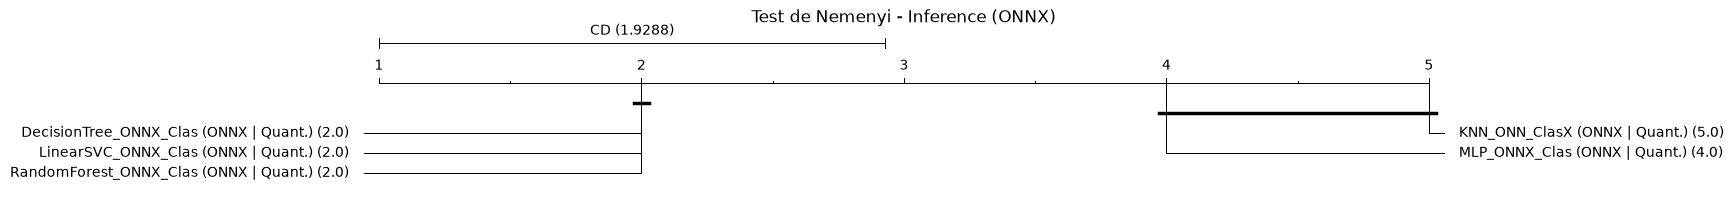
\includegraphics[width=1.0\textwidth]{onnx_nemenyi_inference.png}
    \caption{Diagrama de distancia crítica de Nemenyi para los modelos ONNX en clasificación según el tiempo de inferencia.}
    \label{fig:onnx_nemenyi_inference}
\end{figure}

La latencia presenta el fenómeno estadístico más revelador del estudio. En el gráfico de rangos de Friedman, se produce un
triple empate perfecto (rango 2.0) entre Decision Tree, LinearSVC y Random Forest, situándolos al mismo nivel de velocidad
sin fallo alguno, ya que todos ellos se ejecutan con el menor tiempo medido en este caso, como se comentó anteriormente.\\

El test de Nemenyi muestra que este bloque unificado es significativamente más veloz que MLP (4.0) y k-NN (5.0). Esto
certifica que, gracias a la destilación y al motor en C++, la inferencia de un Random Forest colapsa al límite físico
inferior del hardware, volviéndose estadísticamente indistinguible de los algoritmos de ramificación simple o producto
escalar directo, teniendo en cuenta la grave degradación que ha sufrido al verse reducido a un árbol estudiante.

\subsubsection{scikit-learn vs. ONNX}
LinearSVC resulta ser el algoritmo más resiliente y eficiente del estudio. Mantiene intacto el 100\% de su capacidad
predictiva base (F1 = 0.84554), a la vez que su tamaño se ve reducido en casi un $50\%$ y su velocidad de inferencia se
incrementa por un factor de $18$.
\newpage
\begin{table}[htbp]
  \centering
  \begin{tabularx}{\textwidth}{lXccc}
    \hline
    \textbf{Algoritmo} & \textbf{Framework / Configuración} & \textbf{F1} & \textbf{Inferencia (ms)} & \textbf{Tamaño (KB)} \\
    \hline
    \textbf{DecisionTree} & scikit-learn & 0.82853 & 0.059  & 49.92061   \\
                          & ONNX quant.  & 0.77330 & 0.01   & 30.98779   \\
    \hline
    \textbf{KNeighbors}   & scikit-learn & 0.83775 & 1.162  & 6485.99521 \\
                          & ONNX quant.  & 0.59189 & 0.515  & 241.19912  \\
    \hline
    \textbf{LinearSVC}    & scikit-learn & 0.84554 & 0.18   & 14.31367   \\
                          & ONNX quant.  & 0.84554 & 0.01   & 8.08135    \\
    \hline
    \textbf{MLP}          & scikit-learn & 0.88738 & 0.231  & 126.65029  \\
                          & ONNX quant.  & 0.81938 & 0.023  & 14.34600   \\
    \hline
    \textbf{RandomForest} & scikit-learn & 0.87371 & 14.001 & 1070.22705 \\
                          & ONNX quant.  & 0.72860 & 0.01   & 8.09229    \\
    \hline
  \end{tabularx}
  \caption{Comparativa de rendimiento y coste de algoritmos tradicionales (scikit-learn frente a ONNX) en clasificación.}
  \label{tab:sklearn_onnx_clas_resumen}
\end{table}
A pesar de obtener mejoras en eficiciencia, los resultados muestran que, la poda o la
cuantización, o bien ambas, no están siendo aplicadas al modelo al mantener la exactitud de la predicción. Esto sugiere
que LinearSVC no admite reducciones de este tipo.\\

La transformación de Random Forest representa el mayor sacrificio algorítmico. Su destilación a árbol estudiante sumada a
la cuantización le cuestan una notable degradación predictiva ($\sim14.5\%$ de pérdida en F1). A cambio, el modelo reduce
su tamaño en más de un $99.2\%$ (de 1070 KB a 8 KB) y se acelera por un asombroso factor de $\times 1400$. Transforma un
modelo inasumible para el IoT estricto en una solución instantánea y microscópica.\\

La poda y cuantización del MLP demuestran un excelente balance general. A cambio de ceder menos de un $7\%$ de su F1
original, la red se comprime un $88\%$ en disco y acelera su respuesta en un orden de magnitud. Por su parte, Decision
Tree muestra un comportamiento similar.\\

k-NN fracasa en su transición a sistemas embebidos. La reducción de prototipos, necesaria para evitar que el tamaño se
desborde, destruye por completo su F1-score ($0.83 \rightarrow 0.59$), sin llegar a igualar la ligereza ni la extrema
velocidad de los modelos paramétricos evaluados.\\

Para evitar una saturación de figuras, en esta comparativa solo se muestran los diagramas de distancia crítica de Nemenyi,
ya que se han hallado diferencias significativas en todos los tests de Friedman e Iman-Davenport en las tres métricas.\\

\begin{figure}[htbp]
    \centering
    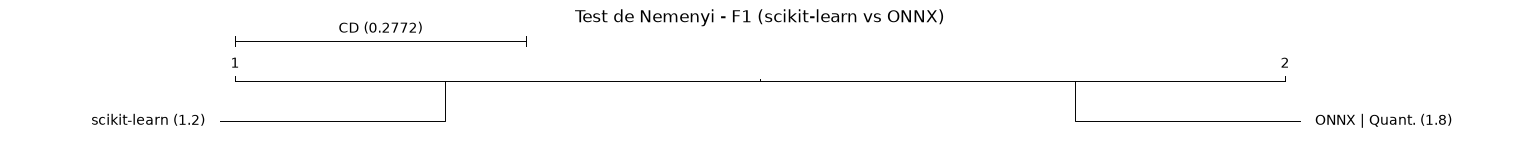
\includegraphics[width=1.0\textwidth]{sklearn_vs_onnx_nemenyi_f1.png}
    \caption{Diagrama de distancia crítica de Nemenyi para los modelos ONNX frente a scikit-learn en clasificación según F1-score.}
    \label{fig:skelearn_vs_onnx_nemenyi_f1}
\end{figure}
\begin{figure}[htbp]
    \centering
    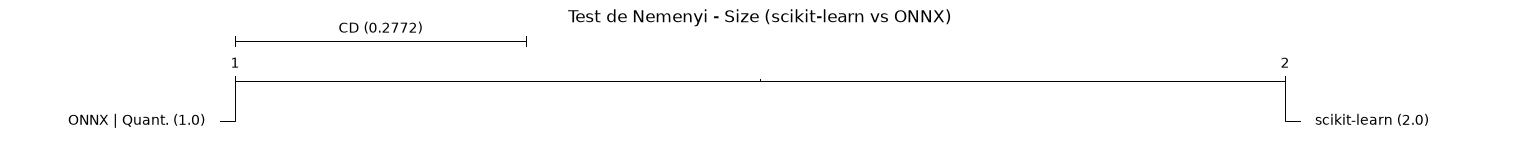
\includegraphics[width=1.0\textwidth]{sklearn_vs_onnx_nemenyi_size.png}
    \caption{Diagrama de distancia crítica de Nemenyi para los modelos ONNX en clasificación según el tamaño del modelo.}
    \label{fig:skelearn_vs_onnx_nemenyi_size}
\end{figure}
\begin{figure}[htbp]
    \centering
    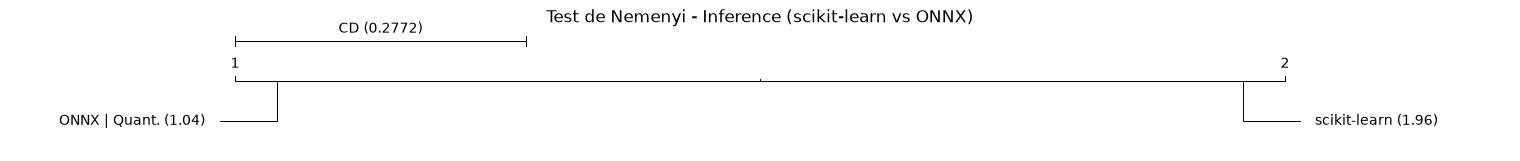
\includegraphics[width=1.0\textwidth]{sklearn_vs_onnx_nemenyi_inference.png}
    \caption{Diagrama de distancia crítica de Nemenyi para los modelos ONNX en clasificación según el tiempo de inferencia.}
    \label{fig:skelearn_vs_onnx_nemenyi_inference}
\end{figure}

Los tests demuestran que la caída del F1-score no es fortuita. Scikit-learn retiene una superioridad estadísticamente
significativa frente a ONNX, debido a la pérdida producida por las técnicas de compresión implementadas. A cambio,
dictaminan una victoria absoluta para ONNX en lo que respecta al tamaño del modelo. La compresión logra el rango ideal
matemático, siendo invariablemente más ligera en cada evaluación. En latencia computacional, el test confirma la misma
tendencia. Con una diferencia de rangos ampliamente superior a la distancia crítica, la ejecución mediante cuantización
y ONNX Runtime garantiza una aceleración estadísticamente incontestable para sistemas en tiempo real.

\subsubsection{Regresión}
De manera análoga a la clasificación, los modelos de regresión han sido sometidos a un pipeline de compresión algorítmica
previo a su exportación y cuantización. Las técnicas aplicadas abarcan desde la poda paramétrica (sparsity para regresión
lineal y MLP, y poda de impurezas paramétricas para Decision Tree), hasta la reducción espacial de prototipos mediante
clustering (k-NN) y la destilación de conocimiento para ensamblados (Random Forest). A continuación, se analiza el
comportamiento interno de este ecosistema optimizado.

\subsubsection{Rendimiento predictivo (R$^2$)}
El hito más llamativo en este escenario es el colapso catastrófico (-4.90574). Mientras que en clasificación la red
soportó la poda y la cuantización (porque la salida final pasa por una función de activación acotada como coftmax o
sigmoid), en regresión la salida es continua y no acotada. Anular los pesos menores a $10^{-4}$ y forzar la representación
de las activaciones a enteros de 8 bits destruye la escala paramétrica de la red. Esto provoca que las predicciones
diverjan bastante de la varianza real de los datos, obteniendo un R$^2$ negativo que invalida al modelo. Cabe destacar que
esto no es un comportamiento generalizado del MLP, sino que se da únicamente para ciertos datasets. Estos conjuntos de
datos presentan una distribución de valores que hace que la cuantización y la poda de pesos afecten de manera más drástica
a la capacidad de predicción del modelo, llevándolo a un estado de ineficacia que no lo hace aplicable en todos los casos.
\newpage
\begin{table}[htbp]
  \centering
  \small
  \begin{tabularx}{\textwidth}{l *{5}{>{\centering\arraybackslash}X}}
    \hline
    \textbf{Dataset} & \textbf{DT} & \textbf{k-NN} & \textbf{LinReg} & \textbf{MLP} & \textbf{RF} \\
    \hline
    ABALONE                      & 0.31095 & 0.47151 & 0.52797 & 0.45932   & 0.50078 \\
    AIR QUALITY                  & 0.83286 & 0.67685 & 0.85493 & 0.84274   & 0.84743 \\
    APPLIANCES ENERGY PREDICTION & 0.64248 & 0.68334 & 0.62108 & 0.49936   & 0.68880 \\
    AUTOMOBILE                   & 0.84311 & 0.42528 & 0.84668 & 0.67090   & 0.86918 \\
    BIKE SHARING HOURLY          & 0.89224 & 0.54878 & 0.38781 & 0.70451   & 0.70381 \\
    COMMUNITIES AND CRIME        & 0.30799 & 0.57029 & 0.65104 & 0.49181   & 0.54685 \\
    OBESITY LEVELS               & 0.98418 & 0.88523 & 0.56080 & -0.80837  & 0.97475 \\
    REAL ESTATE VALUATION        & 0.49584 & 0.49948 & 0.57181 & -8.44344  & 0.64164 \\
    STUDENT PERFORMANCE          & 0.76874 & 0.57664 & 0.79570 & 0.65416   & 0.80021 \\
    WINE QUALITY                 & 0.21155 & 0.12021 & 0.27424 & -44.1284  & 0.33044 \\
    \hline
    \textbf{Media global} & \textbf{0.62899} & \textbf{0.54576} & \textbf{0.60921} & \textbf{-4.90574} & \textbf{0.69039} \\
    \hline
  \end{tabularx}
  \caption{R$^2$ por dataset para los modelos ONNX $+$ cuantización en regresión.}
  \label{tab:onnx_est_r2}
\end{table}

Por el contrario, el árbol destilado del Random Forest (0.69039) y el Decision Tree original podado (0.62899) exhiben una
notable robustez. El éxito del Random Forest demuestra que la destilación de conocimiento es altamente efectiva en
regresión: el árbol estudiante es capaz de aprender y replicar fielmente los patrones de decisión continuos del bosque
original.\\

La Regresión Lineal (0.60921) mantiene una estabilidad absoluta, demostrando que coeficientes inferiores a $10^{-4}$
carecen de impacto predictivo real y que los hiperplanos son matemáticamente resilientes a la cuantización, aunque
no logra un rendimiento superior al de los modelos basados en árboles. Finalmente, el k-NN (0.54576) sufre una pérdida de
precisión esperable al reducir el espectro continuo de datos a un máximo de 200 centroides sintéticos.\\

\begin{figure}[htbp]
    \centering
    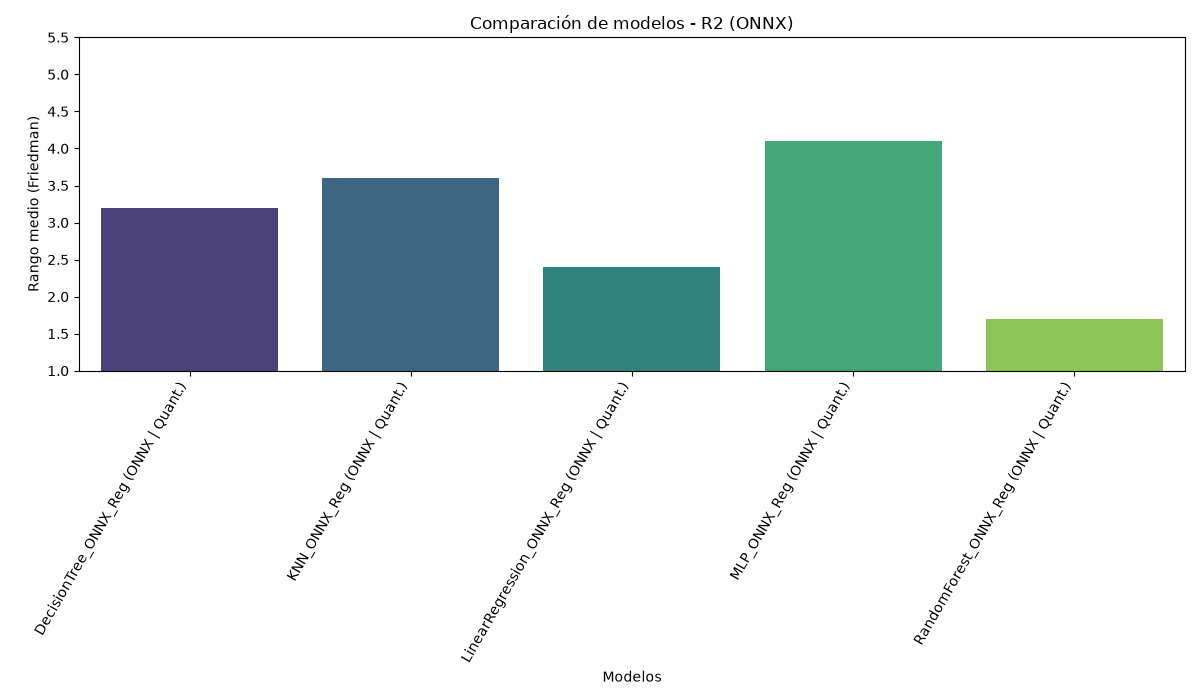
\includegraphics[width=0.808\textwidth]{onnx_reg_average_ranks_r2.png}
    \caption{Rangos medios de los modelos ONNX en regresión según R$^2$.}
    \label{fig:onnx_ranks_r2}
\end{figure}
\begin{figure}[htbp]
    \centering
    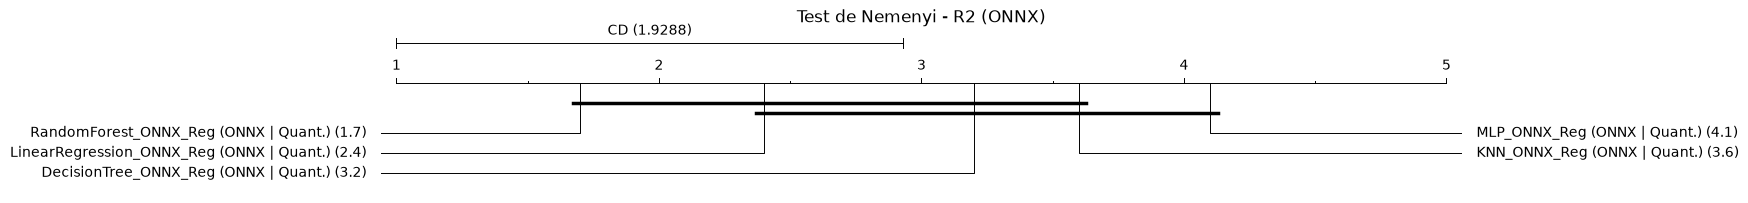
\includegraphics[width=1.0\textwidth]{onnx_reg_nemenyi_r2.png}
    \caption{Diagrama de distancia crítica de Nemenyi para los modelos ONNX en regresión según R$^2$.}
    \label{fig:onnx_nemenyi_r2}
\end{figure}

El análisis global ($p\text{-valor} = 0.0055$) dictamina la existencia de diferencias significativas en la retención de
varianza tras la compresión. Los rangos medios ratifica que el Random Forest destilado lidera la tabla con un rango de
1.7, seguido de cerca por la Regresión Lineal (2.4).\\

El diagrama de distancia crítica confirma estadísticamente lo evidenciado en las métricas previas: el Random Forest es
significativamente superior al MLP (4.1) y al k-NN (3.6). Esto demuestra que, al menos en regresión, la destilación del
Random Forest en un árbol estudiante conserva una capacidad de generalización superior frente al intento de aplicar
cuantización a una red densa o calcular distancias sobre prototipos reducidos en un espectro continuo.

\subsubsection{Huella de memoria (tamaño en disco en KB)}
\begin{table}[htbp]
  \centering
  \small
  \begin{tabularx}{\textwidth}{l *{5}{>{\centering\arraybackslash}X}}
    \hline
    \textbf{Dataset} & \textbf{DT} & \textbf{k-NN} & \textbf{LinReg} & \textbf{MLP} & \textbf{RF} \\
    \hline
    ABALONE                      & 37.08105 & 11.88086 & 0.47070 & 7.39160  & 5.08691 \\
    AIR QUALITY                  & 51.25000 & 46.90527 & 1.10352 & 9.15723  & 5.08691 \\
    APPLIANCES ENERGY PREDICTION & 44.54688 & 32.06152 & 0.82520 & 8.37793  & 5.08691 \\
    AUTOMOBILE                   & 9.20020  & 7.63770  & 1.41113 & 10.01855 & 5.08691 \\
    BIKE SHARING HOURLY          & 67.93262 & 14.87109 & 0.50000 & 7.47363  & 5.08691 \\
    COMMUNITIES AND CRIME        & 29.46484 & 35.88086 & 1.79199 & 11.08496 & 5.08691 \\
    OBESITY LEVELS               & 7.21973  & 13.89746 & 0.72266 & 8.09082  & 5.08691 \\
    REAL ESTATE VALUATION        & 14.68457 & 5.15527  & 0.41211 & 7.22754  & 5.08691 \\
    STUDENT PERFORMANCE          & 9.58203  & 8.17480  & 1.17676 & 9.36230  & 5.08691 \\
    WINE QUALITY                 & 25.27441 & 13.86523 & 0.48535 & 7.43262  & 5.08691 \\
    \hline
    \textbf{Media global} & \textbf{29.62363} & \textbf{19.03301} & \textbf{0.88994} & \textbf{8.56172} & \textbf{5.08691} \\
    \hline
  \end{tabularx}
  \caption{Tamaño en disco por dataset para los modelos ONNX $+$ cuantización en regresión.}
  \label{tab:onnx_est_reg_size}
\end{table}
Los resultados confirman el éxito rotundo del pipeline de compresión a nivel de almacenamiento físico.\\

La regresión lineal domina con un tamaño por debajo del kilobyte (0.88 KB de media), convirtiéndose en una función
matemática trivial en memoria. Sin embargo, la auténtica transformación ocurre en el Random Forest (5.08 KB). Al haber
sido destilado en un único árbol estudiante de topología acotada, su representación en el grafo de ONNX es diminuta,
siendo paradójicamente más ligero que el propio Decision Tree original (29.62 KB), el cual retiene ramas más profundas.\\

El k-NN experimenta el efecto directo de la reducción de prototipos. Al sustituir la memorización completa del dataset por
los clústeres generados mediante \path{MiniBatchKMeans}, su tamaño queda acotado a 19.03 KB, rompiendo la dependencia
lineal entre el volumen de datos y el peso del modelo que penalizaba a los algoritmos de evaluación perezosa.\\

\begin{figure}[htbp]
    \centering
    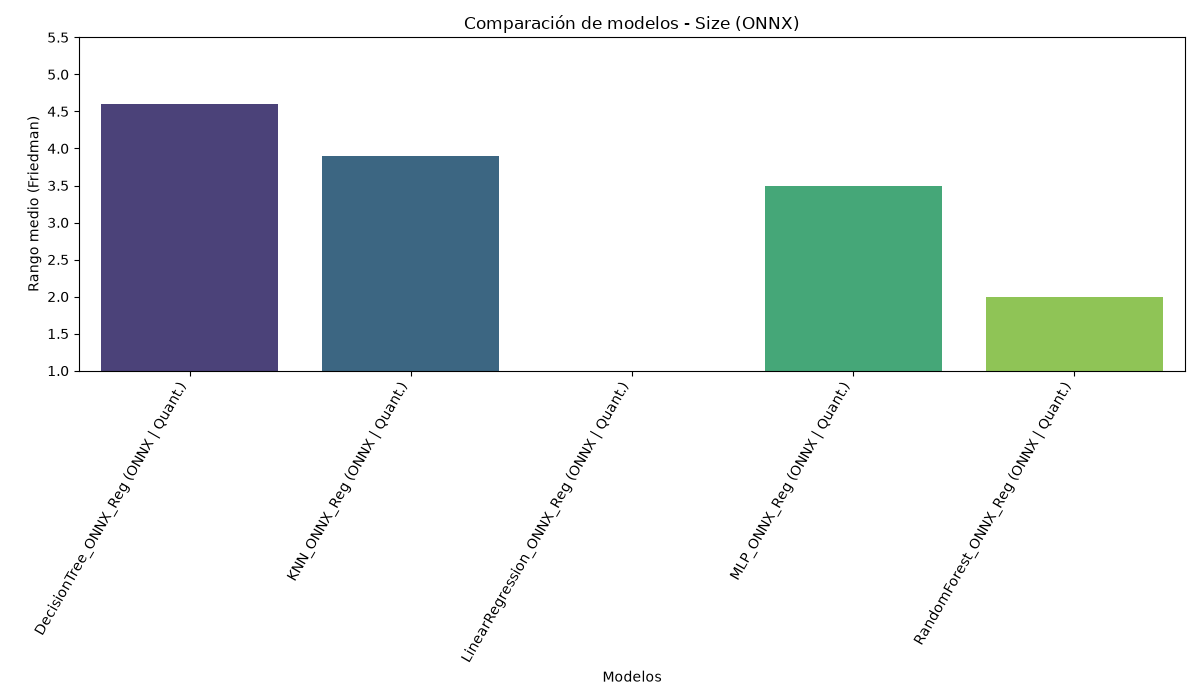
\includegraphics[width=1.0\textwidth]{onnx_reg_average_ranks_size.png}
    \caption{Rangos medios de los modelos ONNX en regresión según el tamaño en disco.}
    \label{fig:onnx_reg_ranks_size}
\end{figure}
\begin{figure}[htbp]
    \centering
    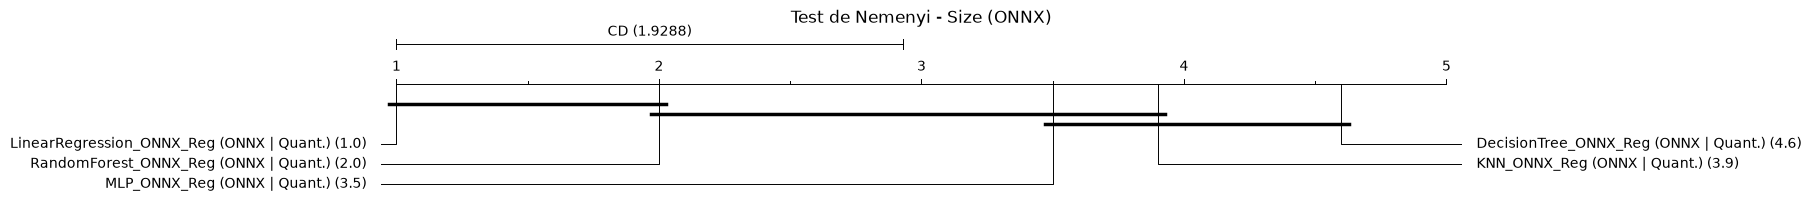
\includegraphics[width=1.0\textwidth]{onnx_reg_nemenyi_size.png}
    \caption{Diagrama de distancia crítica de Nemenyi para los modelos ONNX en regresión según el tamaño en disco.}
    \label{fig:onnx_reg_nemenyi_size}
\end{figure}

La optimización del espacio en disco arroja diferencias drásticas ($p\text{-valor} = 0.000001$). Los rangos de Friedman
establecen a la regresión lineal (1.0) y al Random Forest (2.0) como los indiscutibles ganadores, coincidiendo con lo
analizado previamente.\\

El test de Nemenyi certifica que ambos son estadísticamente más ligeros que el Decision Tree original podado por impureza
(4.6) y el k-NN (3.9). Queda matemáticamente probado que la estrategia aplicada al Random Forest, además de obtener unos
los mejores resultados en rendimiento predictivo, logra la compresión espacial más eficiente. 

\subsubsection{Eficiencia operativa (ms) y resultados globales}
La ejecución en el ecosistema ONNX en C++ vuelve a generar una convergencia radical en la latencia de inferencia.
\newpage
\begin{table}[htbp]
  \centering
  \small
  \begin{tabularx}{\textwidth}{l *{3}{>{\centering\arraybackslash}X}}
    \hline
    \textbf{Modelo} & \textbf{R$^2$} & \textbf{Inferencia (ms)} & \textbf{Tamaño (KB)} \\
    \hline
    DecisionTree    & 0.62899  & 0.01  & 29.62363 \\
    KNeighbors      & 0.54576  & 0.244 & 19.03301 \\
    LinearReg       & 0.60921  & 0.01  & 0.88994  \\
    MLP             & -4.90574 & 0.02  & 8.56172  \\
    RandomForest    & 0.69039  & 0.01  & 5.08691  \\
    \hline
  \end{tabularx}
  \caption{Resumen de eficiencia operativa y coste computacional de los modelos ONNX $+$ cuantización en regresión.}
  \label{tab:onnx_est_reg_resumen}
\end{table}
Decision Tree, regresión lineal y Random Forest comparten un tiempo de ejecución idéntico de 0.01 ms. Es fundamental
comprender que el motor subyacente no está evaluando un bosque de múltiples árboles para el Random Forest, sino
evaluando el único grafo condicional corto derivado de su destilación, igualando así su latencia a la de un modelo lineal
simple. El k-NN, con un tiempo de inferencia de 0.244 ms, sigue siendo un orden de magnitud más lento que los modelos
paramétricos, pues el cálculo de distancias euclídeas, incluso contra un conjunto reducido de 200 centroides, exige
mayor carga de CPU.\\

\begin{figure}[htbp]
    \centering
    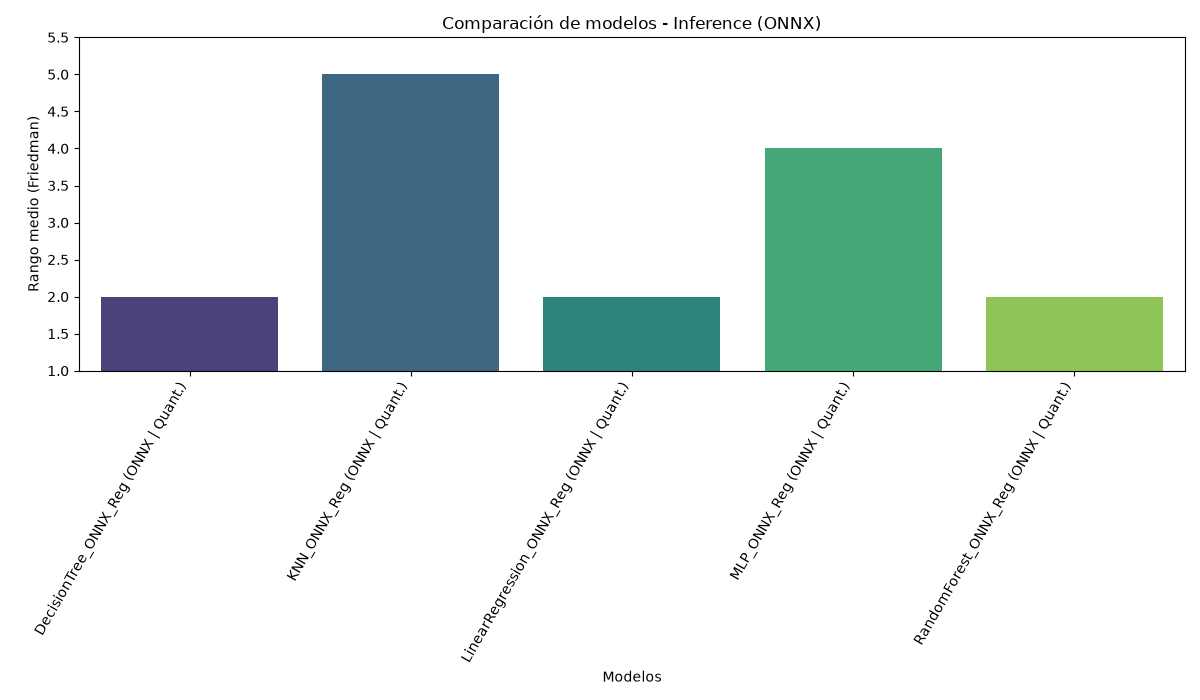
\includegraphics[width=0.9\textwidth]{onnx_reg_average_ranks_inference.png}
    \caption{Rangos medios de los modelos ONNX en regresión según el tiempo de inferencia.}
    \label{fig:onnx_reg_ranks_inference}
\end{figure}
\begin{figure}[htbp]
    \centering
    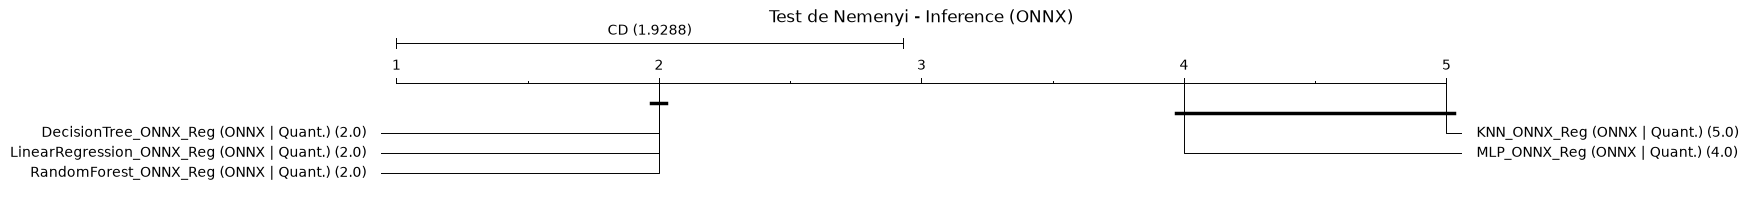
\includegraphics[width=1.0\textwidth]{onnx_reg_nemenyi_inference.png}
    \caption{Diagrama de distancia crítica de Nemenyi para los modelos ONNX en regresión según el tiempo de inferencia.}
    \label{fig:onnx_reg_nemenyi_inference}
\end{figure}

\newpage
La latencia presenta de nuevo un colapso hacia el límite inferior medible por el hardware ($p\text{-valor} = 0.000002$).
Decision Tree, regresión lineal y Random Forest empatan en el rango ideal perfecto (2.0), mientras que k-NN y MLP muestran
una latencia mayor, validando lo observado previamente.\\

Al observar el diagrama de distancia crítica, este bloque unificado se desmarca de manera significativa frente al k-NN
(5.0). La reducción aplicada no logra mitigar la enorme carga computacional inherente al cálculo de distancias euclídeas,
evidenciando que los modelos paramétricos vectorizados en C++ siempre serán estadísticamente superiores en velocidad.

\subsubsection{scikit-learn vs. ONNX}
\begin{table}[htbp]
  \centering
  \begin{tabularx}{\textwidth}{lXccc}
    \hline
    \textbf{Algoritmo} & \textbf{Framework / Configuración} & \textbf{R$^2$} & \textbf{Inferencia (ms)} & \textbf{Tamaño (KB)} \\
    \hline
    \textbf{DecisionTree} & scikit-learn & 0.62899  & 0.055  & 55.25889  \\
                          & ONNX quant.  & 0.62899  & 0.01   & 29.62363  \\
    \hline
    \textbf{KNeighbors}   & scikit-learn & 0.62849  & 0.673  & 800.64717 \\
                          & ONNX quant.  & 0.54576  & 0.244  & 19.03301  \\
    \hline
    \textbf{LinearReg}    & scikit-learn & 0.60921  & 0.153  & 2.06221   \\
                          & ONNX quant.  & 0.60921  & 0.01   & 0.88994   \\
    \hline
    \textbf{MLP}          & scikit-learn & 0.71102  & 0.157  & 38.56562  \\
                          & ONNX quant.  & -4.90574 & 0.02   & 8.56172   \\
    \hline
    \textbf{RandomForest} & scikit-learn & 0.72671  & 14.014 & 983.09521 \\
                          & ONNX quant.  & 0.69039  & 0.01   & 5.08691   \\
    \hline
  \end{tabularx}
  \caption{Comparativa de rendimiento y coste de algoritmos tradicionales (scikit-learn frente a ONNX) en regresión.}
  \label{tab:sklearn_onnx_reg_resumen}
\end{table}
La regresión lineal muestra una transición excelente. Mantiene un R$^2$ idéntico (0.60921), reduce su ya pequeño a menos
de 1 KB, y acelera su respuesta computacional en un factor de $\times 15.3$. Sin embargo, al igual que ocurría en
clasificación con LinearSVC, ni la cuantización ni la poda parecen aplicarse al modelo al no observarse pérdida de
capacidad predictiva. Lo mismo le pasa a Decision Tree: la poda y la cuantización no parecen tener efecto en su
rendimiento, pero ONNX logra reducir su tamaño en un $46.4\%$ y acelerar la inferencia por un factor de $\times 5.5$.\\

La optimización del Random Forest justifica por sí sola el uso de estas técnicas. Cede menos de un $5\%$ de R$^2$
relativo, pero a cambio, el modelo se comprime un $99.4\%$ en disco ($983 \rightarrow 5$ KB) y se acelera por un
asombroso factor de $\times 1400$. Es la mejor muestra en regresión de cómo un modelo inasumible para microcontroladores
puede ser empaquetado para inferencia en tiempo real.\\

El k-NN asume el compromiso geométrico. Pese a que se soluciona su defecto crítico de tamaño, reduciendo su huella de
memoria de 800 KB a 19 KB, la pérdida de capacidad predictiva es significativa y evidente.\\

El MLP muestra la cuantización que la cuantización resulta agresiva en regresión. La destrucción de su precisión descarta
de facto la cuantización combinada con poda en este marco de trabajo.\\

De forma equivalente a como se hizo en clasificación, solo se mostrarán los diagramas de distancia crítica de Nemenyi
para este cara a cara debido a que todos los tests de Friedman e Iman-Davenport han mostrado diferencias significativas
en las tres métricas.\\

\begin{figure}[htbp]
    \centering
    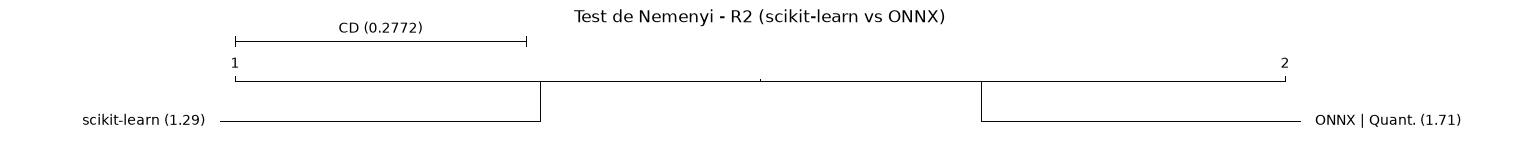
\includegraphics[width=1.0\textwidth]{sklearn_vs_onnx_reg_nemenyi_r2.png}
    \caption{Diagrama de distancia crítica de Nemenyi para los modelos ONNX frente a scikit-learn en regresión según R$^2$.}
    \label{fig:skelearn_vs_onnx_nemenyi_r2}
\end{figure}
\begin{figure}[htbp]
    \centering
    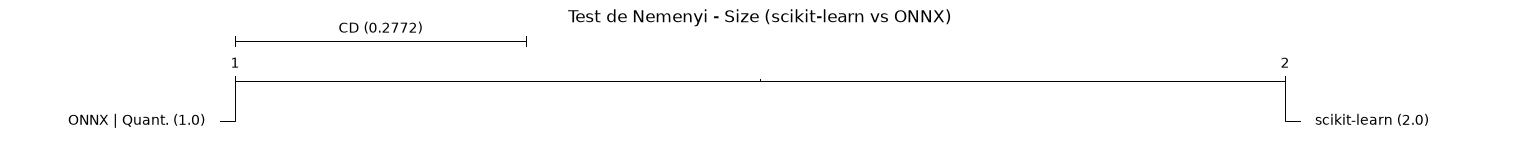
\includegraphics[width=1.0\textwidth]{sklearn_vs_onnx_reg_nemenyi_size.png}
    \caption{Diagrama de distancia crítica de Nemenyi para los modelos ONNX en regresión según el tamaño del modelo.}
    \label{fig:skelearn_vs_onnx_reg_nemenyi_size}
\end{figure}
\begin{figure}[htbp]
    \centering
    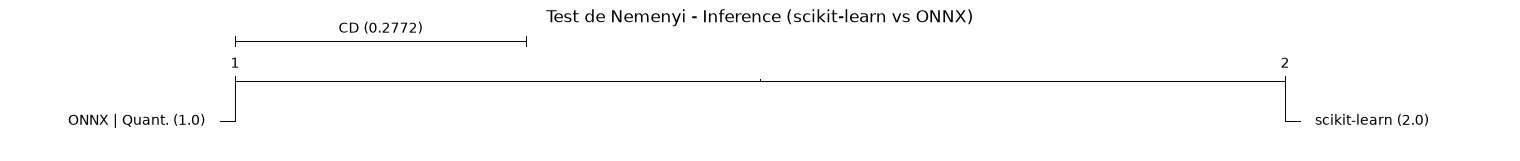
\includegraphics[width=1.0\textwidth]{sklearn_vs_onnx_reg_nemenyi_inference.png}
    \caption{Diagrama de distancia crítica de Nemenyi para los modelos ONNX en regresión según el tiempo de inferencia.}
    \label{fig:skelearn_vs_onnx_reg_nemenyi_inference}
\end{figure}

Los tests realizados documentan una degradación estadísticamente significativa en la capacidad predictiva de los modelos
ONNX. Scikit-learn (1.29) supera a ONNX (1.71) por un margen de 0.42, traspasando la distancia crítica de 0.2772. El
colapso numérico del MLP bajo INT8 es el principal causante de esta penalización global. A pesar de ceder varianza, el
ahorro físico es absoluto. ONNX domina de forma unánime (1.0 vs 2.0), atendiento al diagrama de distancia crítica. La
compresión es sistemáticamente exitosa en todos los datasets evaluados. En latencia, los tests ratifican una superioridad
idéntica (ONNX 1.0 vs scikit-learn 2.0). La ejecución cuantizada es invariable y estadísticamente más rápida, validando
la mayoría de las técnicas implementadas como el estándar viable para el despliegue de estos modelos.

\subsection{PyTorch y TensorFlow}
\subsubsection{Clasificación}
En esta fase se evalúa el comportamiento de arquitecturas neuronales multicapa (MLP) diseñadas e implementadas de forma
nativa en los frameworks de \textit{deep learning} de referencia: PyTorch y TensorFlow (mediante TensorFlow Lite/LiteRT).
Ambos modelos comparten topología paramétrica y son sometidos dos técnicas de compresión distintas: cuantización
post-entrenamiento (PTQ) a 8 bits y destilación de conocimiento, bien combinadas o por separado. El objetivo es determinar
si los ecosistemas nativos gestionan la degradación de precisión y la eficiencia computacional de manera más óptima que la
exportación abordada en las fases previas.\\

En lo que respecta a los tests estadísticos, únicamente se incluirán los diagramas de distancia crítica de Nemenyi, en
caso de que existan diferencias significativas entre los modelos en los tests de Friedman e Iman-Davenport. Igual que ya
se ha hecho antes, el objetivo es mostrar la información relevante sin saturar la lectura con un exceso de figuras.

\subsubsection{Cuantización}
\subsubsection{Rendimiento predictivo (F1-score)}
\begin{table}[htbp]
  \centering
  \small % Reduce ligeramente el tamaño de la fuente para mejorar la legibilidad
  % 'l' para la primera columna de datasets y 'X' para que las de modelos se distribuyan equitativamente
  \begin{tabularx}{\textwidth}{l *{5}{>{\centering\arraybackslash}X}}
    \hline
    \textbf{Dataset} & \textbf{PT quant.} & \textbf{TF quant.} \\
    \hline
    CAR                & 0.98868 & 0.95278 \\
    DIABETES           & 0.67305 & 0.68603 \\
    GAMMA              & 0.85292 & 0.84601 \\
    HAR                & 0.97715 & 0.97479 \\
    IRIS               & 0.95359 & 0.93328 \\
    LETTER RECOGNITION & 0.89430 & 0.88572 \\
    MNIST              & 0.92198 & 0.92355 \\
    SOYBEAN            & 0.95374 & 0.95136 \\
    STUDENT DROPOUT    & 0.64264 & 0.64600 \\
    WINE               & 0.98140 & 0.97461 \\
    \hline
    \textbf{Media global} & \textbf{0.88395} & \textbf{0.87741} \\
    \hline
  \end{tabularx}
  \caption{F1-score por dataset para los modelos de redes neuronales con cuantización en clasificación.}
  \label{tab:nn_quant_f1}
\end{table}
Los resultados demuestran que la cuantización nativa es extremadamente robusta en la preservación de la capacidad de
generalización. Ambos ecosistemas logran un rendimiento casi idéntico, con PyTorch (0.88395) situándose
marginalmente por encima de TensorFlow (0.87741). A diferencia de la caída observada previamente al exportar el MLP de
scikit-learn a ONNX, los motores de cuantización internos de PT y TF logran mapear los tensores de coma flotante a enteros
de 8 bits sin apenas distorsionar los límites de decisión no lineales en conjuntos de datos complejos como \textbf{MNIST}
o \textbf{HAR}.

\newpage
\subsubsection{Huella de memoria (tamaño en disco en KB)}
\begin{table}[htbp]
  \centering
  \small % Reduce ligeramente el tamaño de la fuente para mejorar la legibilidad
  % 'l' para la primera columna de datasets y 'X' para que las de modelos se distribuyan equitativamente
  \begin{tabularx}{\textwidth}{l *{5}{>{\centering\arraybackslash}X}}
    \hline
    \textbf{Dataset} & \textbf{PT quant.} & \textbf{TF quant.} \\
    \hline
    CAR                & 8.94043  & 4.83594  \\
    DIABETES           & 8.50488  & 4.43750  \\
    GAMMA              & 8.56738  & 4.50000  \\
    HAR                & 25.81738 & 21.90625 \\
    IRIS               & 8.38184  & 4.35938  \\
    LETTER RECOGNITION & 9.56934  & 5.73438  \\
    MNIST              & 33.00684 & 29.04688 \\
    SOYBEAN            & 9.88184  & 6.02344  \\
    STUDENT DROPOUT    & 9.38184  & 5.36719  \\
    WINE               & 8.63184  & 4.64844  \\
    \hline
    \textbf{Media global} & \textbf{13.06836} & \textbf{9.08594} \\
    \hline
  \end{tabularx}
  \caption{Tamaño en disco por dataset para los modelos de redes neuronales con cuantización en clasificación.}
  \label{tab:nn_quant_clas_size}
\end{table}
En la optimización del almacenamiento físico, TensorFlow Lite se consolida como la tecnología superior. El formato
\path{.tflite} logra un promedio de 9.08 KB, superando sistemáticamente a PyTorch, con 13.06 KB, en todos los datasets
evaluados. Esta ventaja arquitectónica radica en el uso de \textit{FlatBuffers} por parte de TensorFlow Lite, un sistema
de serialización cruzada diseñado específicamente para maximizar la eficiencia de memoria y permitir el acceso directo a
los datos sin necesidad de desempaquetarlos, ideal para sistemas embebidos.

\subsubsection{Eficiencia operativa (ms), resultados globales y comparativa}
\begin{table}[htbp]
  \centering
  \begin{tabularx}{\textwidth}{lXccc}
    \hline
    \textbf{Framework / Configuración} & \textbf{F1} & \textbf{Inferencia (ms)} & \textbf{Tamaño (KB)} \\
    \hline
    \textbf{scikit-learn}     & 0.88738 & 0.231 & 126.65029 \\
    \hline
    \textbf{ONNX quant.}      & 0.81938 & 0.023 & 14.34600  \\
    \hline
    \textbf{PT quant.}        & 0.88395 & 0.174 & 13.06836  \\
    \hline
    \textbf{TF quant.}        & 0.87741 & 0.081 & 9.08594   \\
    \hline
  \end{tabularx}
  \caption{Comparativa de rendimiento y coste de redes neuronales con cuantización en clasificación.}
  \label{tab:nn_quant_clas_resumen}
\end{table}
La síntesis expuesta revela compromisos arquitectónicos críticos al enfrentar los frameworks nativos contra scikit-learn y
ONNX
\begin{itemize}
  \item PyTorch y TensorFlow logran recuperar de facto la precisión del modelo original de scikit-learn en FP32. Esto
  evidencia que, si se requiere desplegar una red neuronal cuantizada sin ceder capacidad predictiva, es metodológicamente
  más seguro diseñar y cuantizar el modelo utilizando las API nativas del framework en lugar de recurrir a traductores de
  grafos externos como ONNX.
  \item TensorFlow Lite cuantizado establece el nuevo límite inferior de tamaño para redes neuronales en este estudio
  (9.08 KB), logrando una compresión del $\sim 92.8\%$ respecto al modelo original en Python (126.65 KB). La red de PyTorch
  logra reducir mínimamente el tamaño obtenido por ONNX, pero sigue siendo superado por TensorFlow Lite.
  \item El descubrimiento más crítico reside en los tiempos de inferencia. PyTorch sufre una degradación algo notable,
  registrando una latencia media de 0.174 ms. Esta penalización no se debe a la red neuronal en sí, sino a la sobrecarga
  de su motor de inferencia en CPU. PyTorch exige instanciar dinámicamente un objeto \path{Tensor} en memoria y atravesar
  el \textit{runtime} de TorchScript para cada predicción individual. En escenarios de inferencia unitaria,
  característicos de la computación en el borde, este coste arruina el rendimiento. TensorFlow Lite lo gestiona de forma
  mucho más eficiente, con 0.081 ms, mediante la invocación directa de su intérprete en C++, aunque el motor ONNX Runtime
  (0.023 ms) sigue siendo superior en velocidad pura computacional.\\
\end{itemize}

\begin{figure}[htbp]
    \centering
    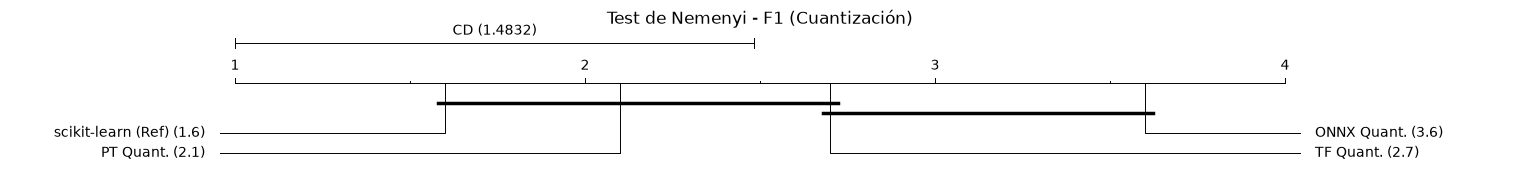
\includegraphics[width=1.0\textwidth]{phase3_quant_nemenyi_f1.png}
    \caption{Diagrama de distancia crítica de Nemenyi para los modelos MLP con cuantización en clasificación según F1-score.}
    \label{fig:nn_quant_nemenyi_f1}
\end{figure}
El análisis global ($p$y-valor = 0.0039) corrobora matemáticamente la superioridad de los motores de cuantización nativos
frente a la exportación genérica. En lo que respecta a la capacidad predictiva, el diagrama de distancia crítica de
Nemenyi arroja información reveladora. No existe diferencia estadística significativa entre el modelo base en coma
flotante y sus versiones cuantizadas nativamente en PT y TF. Sin embargo, ONNX cuantizado cae a la última posición. Queda
probado de forma concluyente que la calibración interna de PyTorch y TensorFlow retienen significativamente más
conocimiento espacial que la traducción del grafo generada por el conversor de ONNX, junto a su respectiva cuantización.\\

\begin{figure}[htbp]
    \centering
    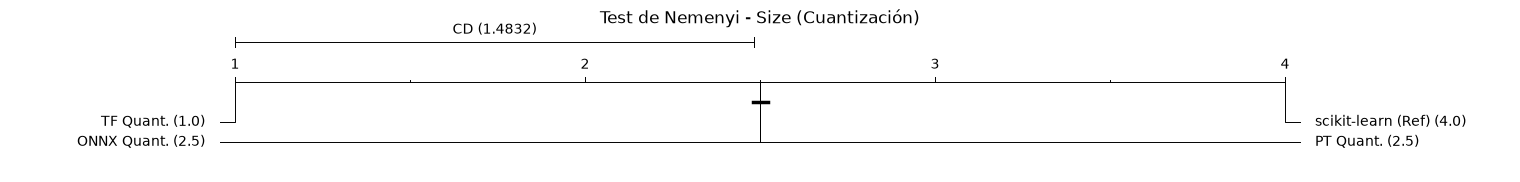
\includegraphics[width=1.0\textwidth]{phase3_quant_nemenyi_size.png}
    \caption{Diagrama de distancia crítica de Nemenyi para los modelos MLP con cuantización en clasificación según el tamaño del modelo.}
    \label{fig:nn_quant_nemenyi_size}
\end{figure}
Nemenyi otorga a TensorFlow Lite la victoria absoluta, con un rango perfecto de 1.0. Se demuestra que TensorFlow es
estadísticamente superior tanto a PyTorch como a ONNX, empatados en rango 2.5. Esto valida matemáticamente la premisa
arquitectónica de TFLite: forzar los tensores estrictamente a \path{tf.int8} y empaquetar el modelo con
\textit{FlatBuffers} produce una compresión significativamente más agresiva y eficiente que la serialización TorchScript
de PyTorch.\\

\begin{figure}[htbp]
    \centering
    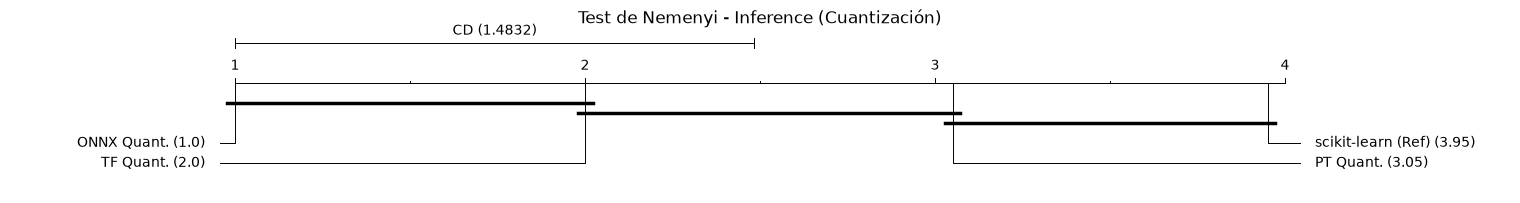
\includegraphics[width=1.0\textwidth]{phase3_quant_nemenyi_inference.png}
    \caption{Diagrama de distancia crítica de Nemenyi para los modelos MLP con cuantización en clasificación según el tiempo de inferencia.}
    \label{fig:nn_quant_nemenyi_inference}
\end{figure}
La distancia crítica de Nemenyi certifica el pequeeño cuello de botella de PyTorch. A pesar de estar cuantizado, el modelo
no logra separarse significativamente del lento modelo original en Python. El \textit{overhead} de inicialización
dinámica de tensores y la invocación del JIT de TorchScript para inferencias individuales hace que la aceleración sea
limitada. Por el contrario, TFLite y ONNX sí se aíslan significativamente del modelo base, demostrando que sus
intérpretes en C++ y C subyacentes son una buena vía en este estudio para garantizar baja latencia.

\subsubsection{Destilación de conocimiento}
A diferencia de la cuantización, cuyo objetivo es reducir la precisión numérica de los pesos para comprimir el modelo
tras el entrenamiento, la destilación de conocimiento (KD, por sus siglas en inglés) interviene directamente en la fase
de optimización. El propósito es enriquecer el mapa de características de una red neuronal ``estudiante'' de topología
reducida (un MLP con capas ocultas [32, 16]) forzándola a imitar no solo las etiquetas reales del conjunto de datos, sino
también las distribuciones de probabilidad continuas (\textit{soft-targets}) generadas por un modelo ``profesor'' de mayor
capacidad paramétrica (un MLP con capas [128, 64, 32]).\\

En esta fase se evalúa el impacto de la destilación operando puramente en coma flotante (FP32), utilizando dos
configuraciones para el hiperparámetro de temperatura: T1 (temperatura = 1.0, equivalente a una función softmax/sigmoide
estándar) y T2 (temperatura = 2.0, que suaviza la distribución de salida).

\subsubsection{Rendimiento predictivo (F1-score)}
Los valores recogidos en esta primera tabla demuestran empíricamente la validez de la destilación como un potente
regularizador activo. En todos los escenarios evaluados, la red estudiante destilada logra igualar o superar el
rendimiento del MLP original instanciado en scikit-learn (0.88738), a pesar de mantener exactamente la misma arquitectura
ligera.
\newpage
\begin{table}[htbp]
  \centering
  \small % Reduce ligeramente el tamaño de la fuente para mejorar la legibilidad
  % 'l' para la primera columna de datasets y 'X' para que las de modelos se distribuyan equitativamente
  \begin{tabularx}{\textwidth}{l *{4}{>{\centering\arraybackslash}X}}
    \hline
    \textbf{Dataset} & \textbf{PT T1} & \textbf{PT T2} & \textbf{TF T1} & \textbf{TF T2} \\
    \hline
    CAR                & 0.98718 & 0.99312 & 0.98960 & 0.99249 \\
    DIABETES           & 0.69482 & 0.70263 & 0.67657 & 0.68781 \\
    GAMMA              & 0.86087 & 0.86039 & 0.85876 & 0.85799 \\
    HAR                & 0.97905 & 0.98012 & 0.98296 & 0.98335 \\
    IRIS               & 0.95554 & 0.94902 & 0.95347 & 0.95121 \\
    LETTER RECOGNITION & 0.90152 & 0.90356 & 0.89922 & 0.90371 \\
    MNIST              & 0.92745 & 0.92946 & 0.92706 & 0.93009 \\
    SOYBEAN            & 0.95849 & 0.95485 & 0.94953 & 0.95501 \\
    STUDENT DROPOUT    & 0.65424 & 0.65972 & 0.66100 & 0.65239 \\
    WINE               & 0.98110 & 0.97953 & 0.97436 & 0.97945 \\
    \hline
    \textbf{Media global} & \textbf{0.89003} & \textbf{0.89124} & \textbf{0.88725} & \textbf{0.88935} \\
    \hline
  \end{tabularx}
  \caption{F1-score por dataset para los modelos de redes neuronales con destilación de conocimiento en clasificación.}
  \label{tab:nn_kd_f1}
\end{table}
El aspecto más destacable del análisis es el impacto del hiperparámetro de temperatura. Tanto en PyTorch como en
TensorFlow, la configuración T2 supera consistentemente, aunque no por un gran margen a T1. En PyTorch, el F1-score medio
asciende de 0.89003 (T1) a 0.89124 (T2), mientras que en TensorFlow evoluciona de 0.88725 a 0.88935. Este comportamiento
valida la teoría fundamental de la destilación: al elevar la temperatura a 2.0, las predicciones del profesor se suavizan,
revelando el ``conocimiento oscuro'' (\textit{dark knowledge})~\cite{hinton2015darkknowledge}. Esto permite al estudiante
aprender las similitudes subyacentes entre clases secundarias (por ejemplo, con qué otra clase se confunde más una muestra
específica), una información rica en gradientes que queda oculta cuando la temperatura es 1.0 y la salida tiende a ser un
vector \textit{one-hot} rígido.

\subsubsection{Huella de memoria (tamaño en disco en KB)}
Dado que la destilación de conocimiento es un proceso que altera exclusivamente la función de pérdida durante la etapa de
entrenamiento, la topología paramétrica del modelo estudiante resultante permanece inalterada (un MLP [32, 16]). Por
consiguiente, la huella de memoria es completamente independiente del hiperparámetro de temperatura (T1 o T2).
\begin{table}[htbp]
  \centering
  \small % Reduce ligeramente el tamaño de la fuente para mejorar la legibilidad
  % 'l' para la primera columna de datasets y 'X' para que las de modelos se distribuyan equitativamente
  \begin{tabularx}{\textwidth}{l *{5}{>{\centering\arraybackslash}X}}
    \hline
    \textbf{Dataset} & \textbf{PT KD} & \textbf{TF KD} \\
    \hline
    CAR                & 8.95410   & 7.00391  \\
    DIABETES           & 7.20605   & 5.33203  \\
    GAMMA              & 7.45801   & 5.58203  \\
    HAR                & 76.58301  & 74.72266 \\
    IRIS               & 6.77051   & 4.91016  \\
    LETTER RECOGNITION & 9.77051   & 7.93750  \\
    MNIST              & 104.70801 & 102.875  \\
    SOYBEAN            & 11.70801  & 9.84766  \\
    STUDENT DROPOUT    & 10.77051  & 8.91016  \\
    WINE               & 7.89551   & 6.03516  \\
    \hline
    \textbf{Media global} & \textbf{25.18242} & \textbf{23.31563} \\
    \hline
  \end{tabularx}
  \caption{Tamaño en disco por dataset para los modelos de redes neuronales con destilación de conocimiento en clasificación.}
  \label{tab:nn_kd_clas_size}
\end{table}
\newpage
La diferencia de tamaños radica únicamente en el motor de serialización del framework. Al operar en FP32, los modelos son
lógicamente más pesados que en la fase de cuantización. Como se observó en el caso de cuantización, TensorFlow Lite
retiene su superioridad arquitectónica en almacenamiento mediante \textit{FlatBuffers}, ocupando una media de 23.31 KB,
frente a los 25.18 KB generados por la exportación a TorchScript en PyTorch. No obstante, ambos ecosistemas logran
comprimir drásticamente el espacio frente al modelo base de Python ($\sim 126$ KB), demostrando que el despliegue nativo
ya implica de por sí una optimización estructural.

\subsubsection{Eficiencia operativa (ms), resultados globales y comparativa}
\begin{table}[htbp]
  \centering
  \begin{tabularx}{\textwidth}{lXccc}
    \hline
    \textbf{Framework / Configuración} & \textbf{F1} & \textbf{Inferencia (ms)} & \textbf{Tamaño (KB)} \\
    \hline
    \textbf{scikit-learn}     & 0.88738 & 0.231 & 126.65029 \\
    \hline
    \textbf{PT T1}            & 0.89003 & 0.137 & 25.18242  \\
    \textbf{PT T2}            & 0.89124 & 0.136 & 25.18242  \\
    \hline
    \textbf{TF T1}            & 0.88725 & 0.071 & 23.31563  \\
    \textbf{TF T2}            & 0.88935 & 0.071 & 23.31563  \\
    \hline
  \end{tabularx}
  \caption{Comparativa de rendimiento y coste de redes neuronales con destilación de conocimiento en clasificación.}
  \label{tab:nn_kd_clas_resumen}
\end{table}
A partir de esta tabla a modo de resumen, se extraen las siguientes conclusiones operativas.
\begin{itemize}
  \item La mejora predicción obtenida (especialmente bajo la configuración T2) no conlleva ningún tipo de penalización
  durante la fase de inferencia. El modelo en producción sigue siendo un MLP ligero que requiere los mismos ciclos de
  reloj y memoria RAM que un modelo entrenado de forma convencional, pero exhibiendo un comportamiento predictivo propio
  de una red neuronal mucho más profunda. Por tanto, diríamos que se tiene una precisión ``gratuita'' en inferencia.
  \item Al operar en FP32 y prescindir de la cuantización, se observa un cambio radical en los tiempos de inferencia de
  PyTorch respecto a fases anteriores. La latencia desciende de 0.174 ms a unos 0.13 ms, demostrando que el
  \textit{overhead} detectado previamente residía en el motor de cuantización, si bien sigue operando más lentamente que
  su contraparte en TensorFlow Lite. Por su parte, este otro framework sigue demostrando una estabilidad computacional
  excelente, manteniendo latencias de 0.071 ms.
\end{itemize}

\newpage
\begin{figure}[htbp]
    \centering
    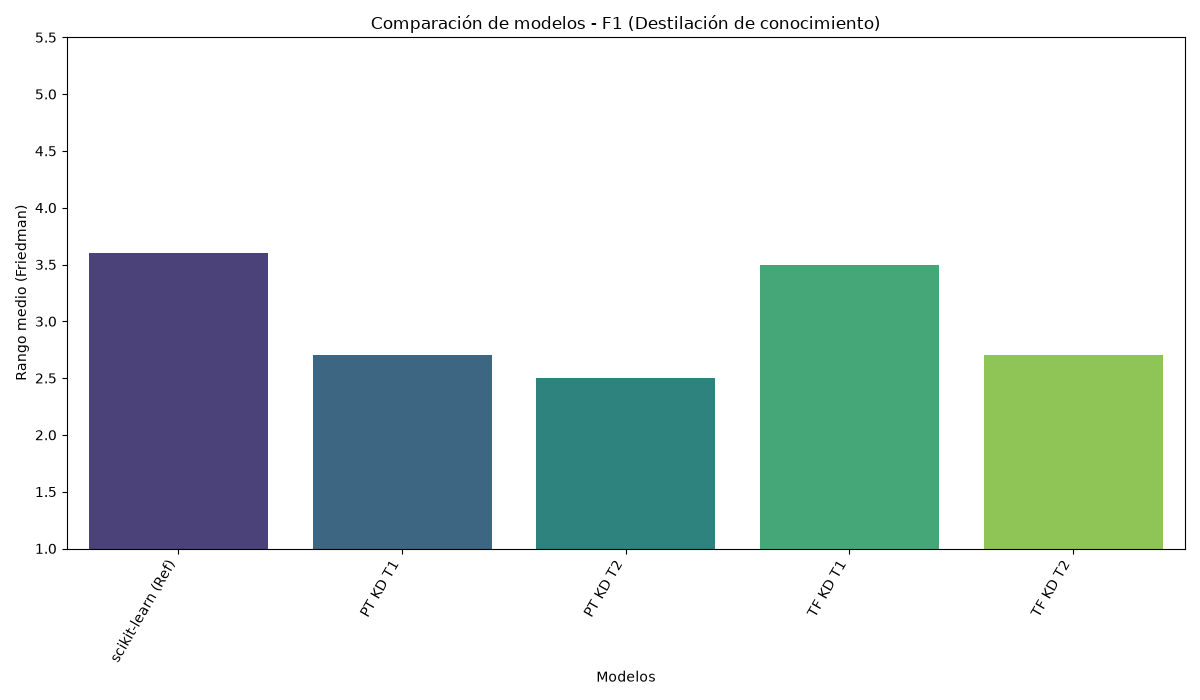
\includegraphics[width=1.0\textwidth]{phase4_distill_average_ranks_f1.png}
    \caption{Rangos medios de los modelos MLP con destilación de conocimiento en clasificación según F1-score.}
    \label{fig:nn_distill_ranks_f1}
\end{figure}
El análisis estadístico de la capacidad predictiva revela que el test de Friedman arroja un $p$-valor de 0.3847, lo que
obliga a mantener la hipótesis nula. Esto significa que, desde un rigor estrictamente matemático, no existen diferencias
estadísticamente significativas en el rendimiento de los modelos a lo largo de los 10 conjuntos de datos, como se observó
previamente de forma teórica. La lectura de los rangos medios confirma la tendencia analizada. El modelo base original de
scikit-learn queda relegado a la última posición con un rango, mientras que la variante destilada en PyTorch con
temperatura 2.0 asume el liderazgo. Aunque la mejora no cruza el umbral de significancia estadística global, el test
confirma que la inyección del \textit{dark knowledge} de Hinton actúa como un método de regularización seguro: en el peor
de los casos, garantiza retener el rendimiento del modelo base, y en el mejor, posiciona a los estudiantes destilados con
$T=2$ como los de mayor rango predictivo.\\

\begin{figure}[htbp]
    \centering
    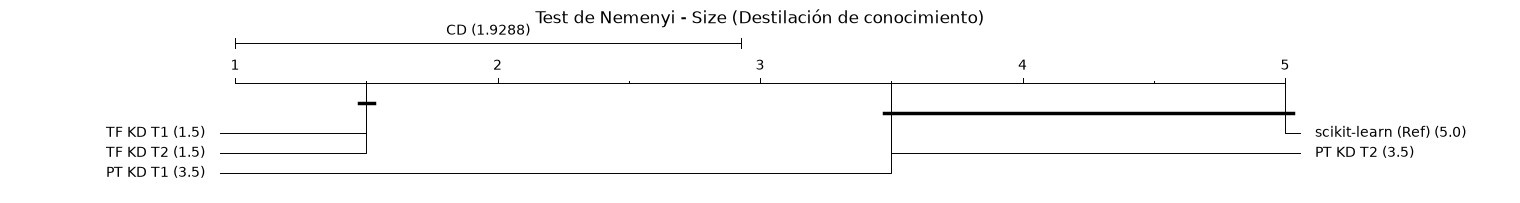
\includegraphics[width=1.0\textwidth]{phase4_distill_nemenyi_size.png}
    \caption{Diagrama de distancia crítica de Nemenyi para los modelos MLP con destilación de conocimiento en clasificación según el tamaño del modelo.}
    \label{fig:nn_distill_nemenyi_size}
\end{figure}
A nivel de optimización espacial, el test rechaza contundentemente la hipótesis nula ($p < 0.001$). Resulta evidente que
el hiperparámetro de temperatura no ejerce ninguna influencia sobre el tamaño final del modelo, otorgando rangos idénticos
a las dos variantes de TensorFlow y a las de PyTorch. Esto es algorítmicamente lógico, ya que la temperatura solo altera
la función de pérdida durante la retropropagación, manteniendo la topología del grafo intacta. Observando el diagrama de
distancia crítica de Nemenyi, TensorFlow logra separarse significativamente de PyTorch, demostrando que la serialización
nativa mediante \textit{FlatBuffers} es matemáticamente más eficiente que el formato TorchScript a la hora de empaquetar
modelos en FP32, mismo comportamiento que se observó en la fase de cuantización.\\

\begin{figure}[htbp]
    \centering
    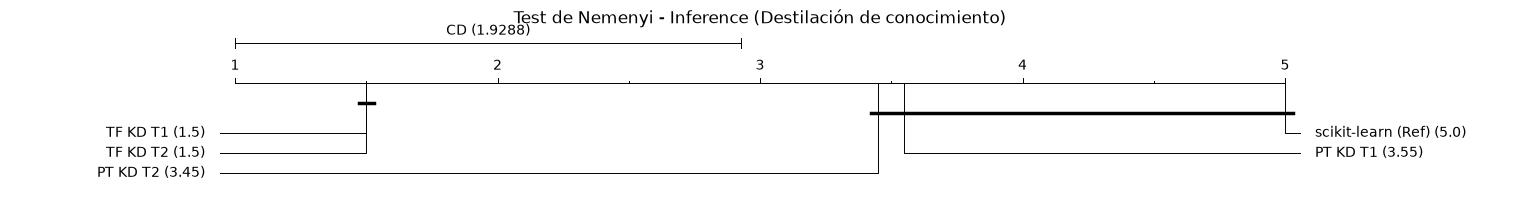
\includegraphics[width=1.0\textwidth]{phase4_distill_nemenyi_inference.png}
    \caption{Diagrama de distancia crítica de Nemenyi para los modelos MLP con destilación de conocimiento en clasificación según el tiempo de inferencia.}
    \label{fig:nn_distill_nemenyi_inference}
\end{figure}
La evaluación de latencias muestra de nuevo un rechazo unánime de la hipótesis nula ($p < 0.001$), posicionando a las
implementaciones de TensorFlow Lite como las más rápidas. El análisis de distancias críticas permite obtener dos
conclusiones fundamentales para el despliegue de estos modelos. En primer lugar, TensorFlow Lite (1.5) es el único framework que
logra una aceleración estadísticamente significativa frente a scikit-learn (5.0) operando en coma flotante. En segundo
lugar, al ejecutar inferencias nativas en FP32 sin el proceso de cuantización, PyTorch logra reducir su cuello de
botella anterior, situándose a una distancia no significativa del modelo base. No obstante, la solidez del motor C++ de
TensorFlow Lite prevalece, logrando incluso distanciarse significativamente de la latencia ofrecida por el intérprete JIT
de PyTorch.

\subsubsection{Cuantización y destilación de conocimiento}
En esta fase se evalúa la aplicación simultánea de ambas técnicas: la compresión numérica mediante cuantización a 8 bits
y el enriquecimiento semántico a través de la destilación de conocimiento, utilizando la misma arquitectura para el
profesor que en la fase previa. El objetivo analítico es determinar si la inyección del \textit{dark knowledge} es capaz
de compensar o mitigar la degradación métrica provocada por la pérdida de precisión en los pesos y activaciones durante el
despliegue.

\newpage
\subsubsection{Rendimiento predictivo (F1)}
\begin{table}[htbp]
  \centering
  \small % Reduce ligeramente el tamaño de la fuente para mejorar la legibilidad
  % 'l' para la primera columna de datasets y 'X' para que las de modelos se distribuyan equitativamente
  \begin{tabularx}{\textwidth}{l *{5}{>{\centering\arraybackslash}X}}
    \hline
    \textbf{Dataset} & \textbf{PT quant. T1} & \textbf{PT quant. T2} & \textbf{TF quant. T1} & \textbf{TF quant. T2} \\
    \hline
    CAR                & 0.98560 & 0.99186 & 0.95286 & 0.96024 \\
    DIABETES           & 0.69575 & 0.69956 & 0.67763 & 0.68836 \\
    GAMMA              & 0.85536 & 0.85554 & 0.85275 & 0.84967 \\
    HAR                & 0.97660 & 0.97925 & 0.98273 & 0.98269 \\
    IRIS               & 0.95554 & 0.94902 & 0.93787 & 0.93560 \\
    LETTER RECOGNITION & 0.89455 & 0.89666 & 0.89323 & 0.89802 \\
    MNIST              & 0.92080 & 0.92642 & 0.92413 & 0.92928 \\
    SOYBEAN            & 0.95916 & 0.95538 & 0.94912 & 0.95468 \\
    STUDENT DROPOUT    & 0.64640 & 0.65388 & 0.65578 & 0.65287 \\
    WINE               & 0.98110 & 0.97953 & 0.97788 & 0.97774 \\
    \hline
    \textbf{Media global} & \textbf{0.88709} & \textbf{0.88871} & \textbf{0.88040} & \textbf{0.88292} \\
    \hline
  \end{tabularx}
  \caption{F1-score por dataset para los modelos de modelos de redes neuronales con cuantización y destilación de conocimiento en clasificación.}
  \label{tab:pt_quant_kd_f1}
\end{table}
En PyTorch, la configuración híbrida con temperatura 2.0 (PT quant. + T2) alcanza un F1-score medio global de 0.88871,
superando no solo a la cuantización pura (0.88395), sino que incluso logra igualar el rendimiento del modelo base de
scikit-learn (0.88738). En TensorFlow, la variante T2 asciende hasta 0.88292, mejorando significativamente los resultados
de la cuantización estándar (0.87741). Este comportamiento corrobora una hipótesis clave: el ruido de discretización
introducido al mapear tensores de FP32 a INT8 distorsiona los gradientes locales, pero el uso de \textit{soft-targets}
suavizados con $T=2$ guía a la red estudiante hacia mínimos más planos y robustos, neutralizando el impacto negativo de la
cuantización.

\subsubsection{Huella de memoria (tamaño en disco en KB)}
\begin{table}[htbp]
  \centering
  \small % Reduce ligeramente el tamaño de la fuente para mejorar la legibilidad
  % 'l' para la primera columna de datasets y 'X' para que las de modelos se distribuyan equitativamente
  \begin{tabularx}{\textwidth}{l *{5}{>{\centering\arraybackslash}X}}
    \hline
    \textbf{Dataset} & \textbf{PT quant. KD} & \textbf{TF quant. KD} \\
    \hline
    CAR                & 8.94043  & 4.83594  \\
    DIABETES           & 8.50488  & 4.45312  \\
    GAMMA              & 8.56934  & 4.51562  \\
    HAR                & 25.81934 & 21.90625 \\
    IRIS               & 8.38184  & 4.36719  \\
    LETTER RECOGNITION & 9.56934  & 5.73438  \\
    MNIST              & 33.00684 & 29.04688 \\
    SOYBEAN            & 9.88184  & 6.02344  \\
    STUDENT DROPOUT    & 9.38184  & 5.36719  \\
    WINE               & 8.63184  & 4.64844  \\
    \hline
    \textbf{Media global} & \textbf{13.06875} & \textbf{9.08984} \\
    \hline
  \end{tabularx}
  \caption{Tamaño en disco por dataset para los modelos de redes neuronales con cuantización y destilación de conocimiento en clasificación.}
  \label{tab:nn_quant_kd_clas_size}
\end{table}
La comparativa de almacenamiento revela una conclusión predecible pero fundamental: la huella de memoria de los modelos
híbridos es exactamente idéntica a la de los modelos sometidos a cuantización pura. Este resultado técnico confirma que la
destilación de conocimiento es estrictamente un paradigma de optimización que opera durante el entrenamiento. Una vez que
la red estudiante ha convergido utilizando la función de pérdida combinada, el modelo profesor se descarta por completo.
Por lo tanto, el artefacto final serializado conserva únicamente la topología compacta del estudiante cuantizado a 8 bits,
logrando la máxima compresión espacial ($\sim 92\%$ de reducción frente al original) sin heredar ninguna sobrecarga
estructural del profesor.

\subsubsection{Resultados globales y comparativa}
La integración de ambas técnicas supone un balance óptimo para despliegues en dispositivos embebidos, consolidando las
siguientes observaciones.
\begin{itemize}
  \item Las configuraciones híbridas demuestran ser una estrategia óptima para entornos con restricciones severas de
  hardware. Permiten dotar a una red de recursos limitados de una capacidad predictiva equivalente a la
  de modelos profundos, sin inflar el tamaño del archivo binario.
  \item Los tiempos de inferencia no se ven afectados por la inclusión de la destilación, ya que dependen exclusivamente
  del motor de ejecución del framework. PyTorch mantiene el su tiempo más elevado (0.174 ms) debido a la sobrecarga de
  despacho dinámico en inferencias unitarias. Por su parte, TensorFlow Lite conserva su agilidad en el rango de los
  0.081 ms gracias a su arquitectura en C++.
  \item El hiperparámetro de T=2 sigue siendo un factor determinante para la robustez de los modelos. En todos los
  escenarios, suavizar las distribuciones del profesor inyecta mayor riqueza relacional entre clases que utilizar un
  $T=1$, dotando a los pesos discretizados de una robustez superior ante anomalías espaciales.
\end{itemize}

\subsubsection{Eficiencia operativa (ms), resultados globales y comparativa en PyTorch}
\begin{table}[htbp]
  \centering
  \begin{tabularx}{\textwidth}{lXccc}
    \hline
    \textbf{Framework / Configuración} & \textbf{F1} & \textbf{Inferencia (ms)} & \textbf{Tamaño (KB)} \\
    \hline
    \textbf{scikit-learn}     & 0.88738 & 0.231 & 126.65029 \\
    \hline
    \textbf{PT quant.}        & 0.88395 & 0.174 & 13.06836 \\
    \textbf{PT T1}            & 0.89003 & 0.137 & 25.18242 \\
    \textbf{PT T2}            & 0.89124 & 0.136 & 25.18242 \\
    \textbf{PT quant. $+$ T1} & 0.88709 & 0.172 & 13.06875 \\
    \textbf{PT quant. $+$ T2} & 0.88871 & 0.174 & 13.06875 \\
    \hline
  \end{tabularx}
  \caption{Comparativa de rendimiento y coste de redes neuronales en PyTorch con cuantización y destilación de conocimiento en clasificación.}
  \label{tab:pytorch_quant_kd_clas_resumen}
\end{table}

\newpage
\begin{figure}[htbp]
    \centering
    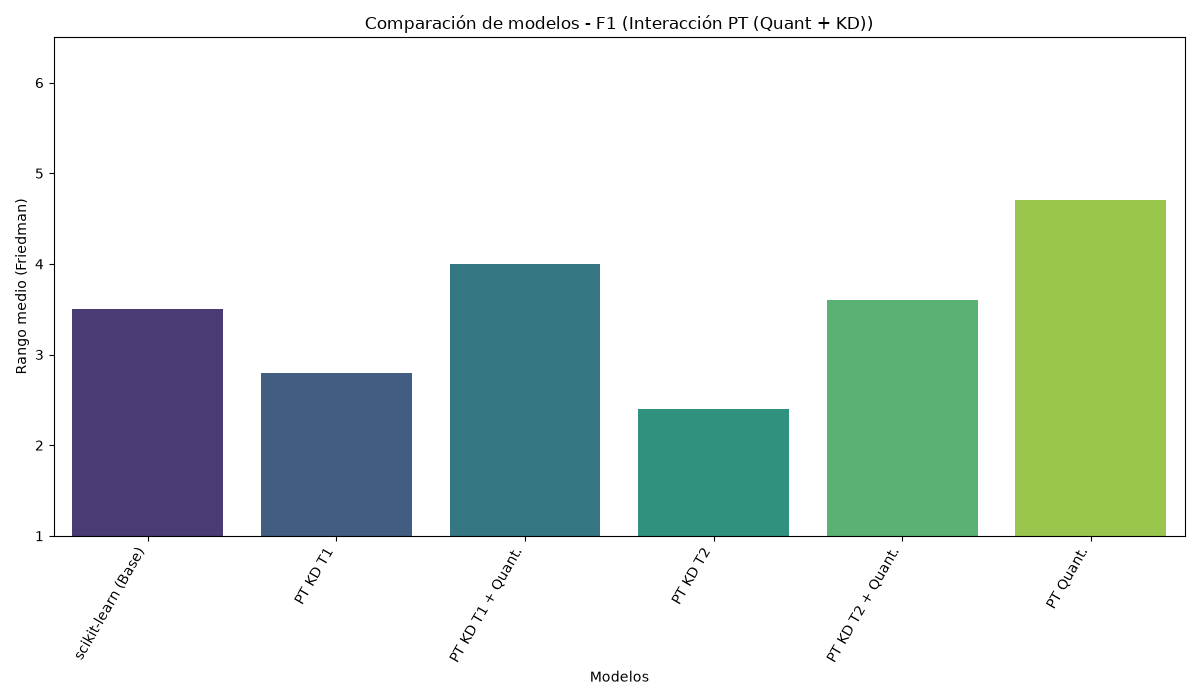
\includegraphics[width=1.0\textwidth]{phase5_pytorch_average_ranks_f1.png}
    \caption{Rangos medios de los modelos PyTorch con cuantización y destilación de conocimiento en clasificación según F1-score.}
    \label{fig:pt_quant_kd_ranks_f1}
\end{figure}
En PyTorch, el test de Friedman arroja un $p$-valor de 0.0837, por lo que no se detectan diferencias estadísticamente
significativas a nivel global entre las distribuciones. Sin embargo, la inspección visual de los rangos medios confirma
la hipótesis teórica: el modelo cuantizado puro (PT Quant.) cae a la última posición con un rango de 4.7. Al integrar la
destilación (PT KD T2 + Quant.), el modelo escala posiciones hasta un rango de 3.6, situándose a nivel práctico en un
empate técnico con el modelo original de scikit-learn (3.5). Aún así, las configuraciones que obtienen el mejor
rendimiento predictivo son aquellas en las que se emplea únicamente la destilación de conocimiento, ya que la precisión
numérica no se ve comprometida por la cuantización.\\

\begin{figure}[htbp]
    \centering
    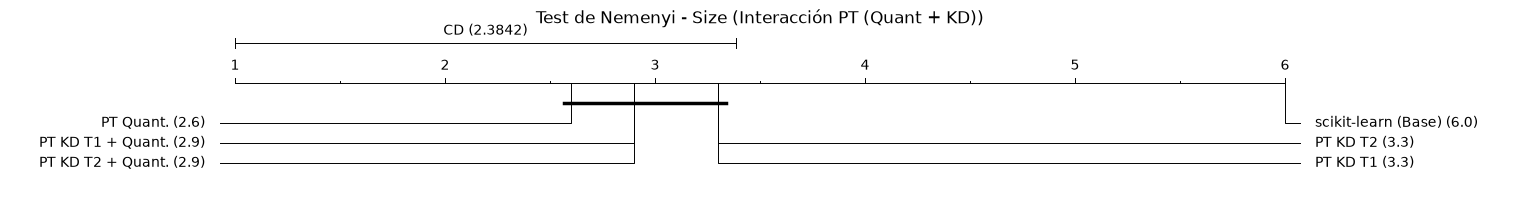
\includegraphics[width=1.0\textwidth]{phase5_pytorch_nemenyi_size.png}
    \caption{Diagrama de distancia crítica de Nemenyi para los modelos PyTorch con cuantización y destilación de conocimiento en clasificación según el tamaño en disco.}
    \label{fig:pt_quant_kd_nemenyi_size}
\end{figure}
La compresión de almacenamiento rechaza unánimemente la hipótesis nula ($p < 0.001$). El diagrama de distancia crítica
certifica que ninguna diferencia significativa entre cuantizar de forma estándar y añadir destilación, aunque queda
patente el efecto compresor de la cuantización. Ambos bloques se aíslan significativamente del modelo base de Python.\\

\newpage
\begin{figure}[htbp]
    \centering
    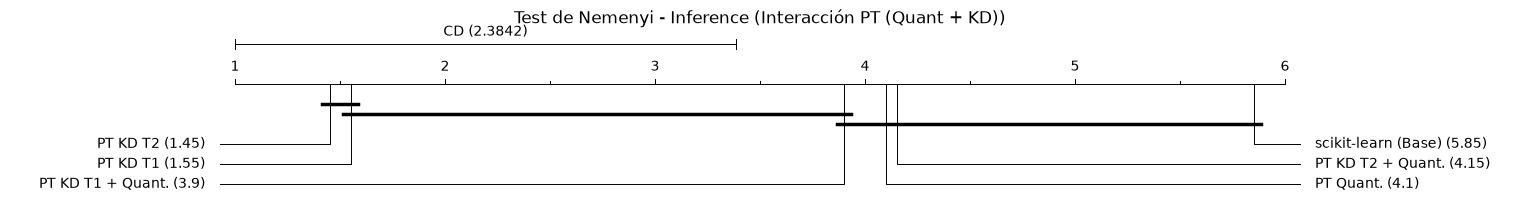
\includegraphics[width=1.0\textwidth]{phase5_pytorch_nemenyi_inference.png}
    \caption{Diagrama de distancia crítica de Nemenyi para los modelos PyTorch con cuantización y destilación de conocimiento en clasificación según el tiempo de inferencia.}
    \label{fig:pt_quant_kd_nemenyi_inference}
\end{figure}
El análisis de la latencia (ambos con $p < 0.001$) expone un fenómeno interesante inherente a los motores de ejecución. En
este caso, los modelos híbridos y los puros se agrupan estadísticamente en un mismo bloque de rangos, lo que confirma que
aplicar destilación no penaliza en absoluto la velocidad de ejecución frente a un modelo estándar cuantizado. Los modelos
que lideran el ranking son las variantes destiladas puras en FP32, lo que da a entender que, en el hardware de ejecución,
el flujo de tensores continuos es una ruta más rápida que la conversión a INT8, aunque la diferencia no sea significativa
de forma generalizada.

\subsubsection{Eficiencia operativa (ms), resultados globales y comparativa en TensorFlow}
\begin{table}[htbp]
  \centering
  \begin{tabularx}{\textwidth}{lXccc}
    \hline
    \textbf{Framework / Configuración} & \textbf{F1} & \textbf{Inferencia (ms)} & \textbf{Tamaño (KB)} \\
    \hline
    \textbf{scikit-learn}     & 0.88738 & 0.231 & 126.65029 \\
    \hline
    \textbf{TF quant.}        & 0.87741 & 0.081 & 9.08594  \\
    \textbf{TF T1}            & 0.88725 & 0.071 & 23.31563 \\
    \textbf{TF T2}            & 0.88935 & 0.071 & 23.31563 \\
    \textbf{TF quant. $+$ T1} & 0.88040 & 0.081 & 9.08984  \\
    \textbf{TF quant. $+$ T2} & 0.88292 & 0.081 & 9.08984  \\
    \hline
  \end{tabularx}
  \caption{Comparativa de rendimiento y coste de redes neuronales en TensorFlow con cuantización y destilación de conocimiento en clasificación.}
  \label{tab:tflite_quant_kd_clas_resumen}
\end{table}

\begin{figure}[htbp]
    \centering
    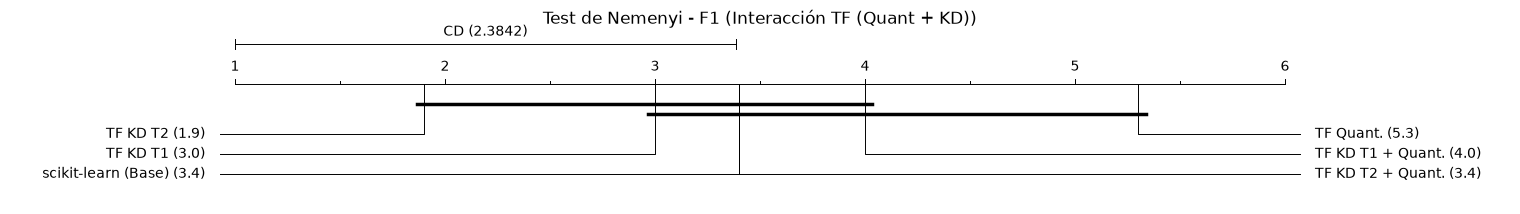
\includegraphics[width=1.0\textwidth]{phase6_tensorflow_nemenyi_f1.png}
    \caption{Diagrama de distancia crítica de Nemenyi para los modelos TensorFlow con cuantización y destilación de conocimiento en clasificación según el tiempo de inferencia.}
    \label{fig:tf_quant_kd_nemenyi_f1}
\end{figure}
A diferencia de PyTorch, el test de Friedman en TensorFlow rechaza la hipótesis nula ($p = 0.0028$). El diagrama de
distancia crítica revela que mientras que el modelo con cuantización pura (TF Quant.) obtiene el peor rango, alejándose de
las variantes en coma flotante, como era de esperar, al inyectar el conocimiento del profesor, la variante híbrida (TF KD
T2 + Quant.) asciende y logra empatar matemáticamente con el modelo base de scikit-learn y pelear con los modelos
destilados puros. Esto confirma estadísticamente que el uso de \textit{soft-targets} compensa la pérdida de información
topológica inducida por el truncamiento a INT8.

\begin{figure}[htbp]
    \centering
    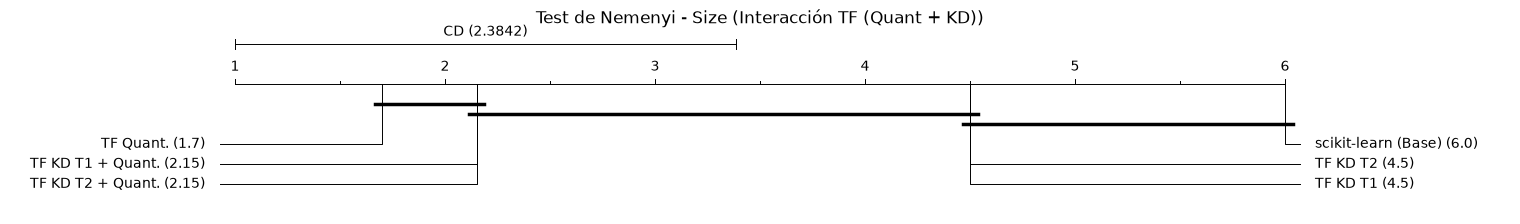
\includegraphics[width=1.0\textwidth]{phase6_tensorflow_nemenyi_size.png}
    \caption{Diagrama de distancia crítica de Nemenyi para los modelos TensorFlow con cuantización y destilación de conocimiento en clasificación según el tiempo de inferencia.}
    \label{fig:tf_quant_kd_nemenyi_size}
\end{figure}
Los tests de Friedman e Iman-Davenport también rechazan la hipótesis nula en TensorFlow ($p < 0.001$). En este caso, se
replica el patrón observado en PyTorch pero con mayor agresividad. Las variantes híbridas conforman junto a la
cuantización pura el bloque más eficiente, probando de forma concluyente que la etapa de entrenamiento con el profesor no
transfiere ni un solo byte de sobrecarga a la arquitectura estudiante una vez serializada.

\begin{figure}[htbp]
    \centering
    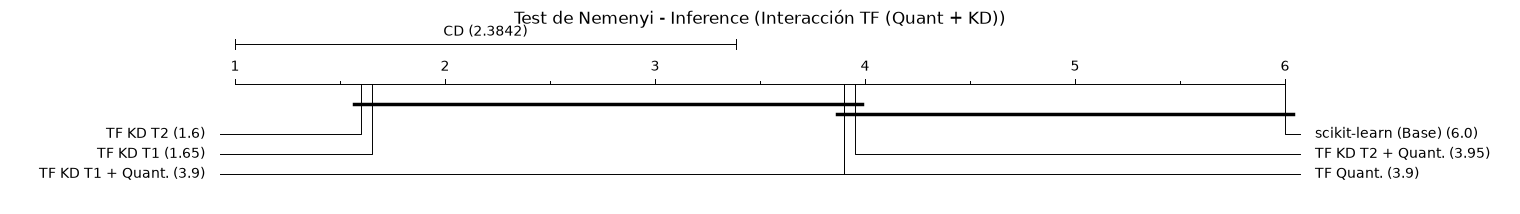
\includegraphics[width=1.0\textwidth]{phase6_tensorflow_nemenyi_inference.png}
    \caption{Diagrama de distancia crítica de Nemenyi para los modelos TensorFlow con cuantización y destilación de conocimiento en clasificación según el tiempo de inferencia.}
    \label{fig:tf_quant_kd_nemenyi_inference}
\end{figure}
El comportamiento de la latencia en TensorFlow Lite es similar al de PyTorch. Los modelos con solo destilación vuelven a
ser los líderes, siendo en este caso estadísticamente significativos frente a los modelos híbridos y a la cuantización
pura, pero demostrando aún que representan una alternativa algo más rápida.

\subsubsection{Regresión}
La fase correspondiente a regresión se estructura de forma análoga a la de clasificación, usando las mismas arquitecturas
tanto en PyTorch como en TensorFlow, adaptadas a la naturaleza de salida continua de los problemas de regresión. De la
misma forma, se aplican las técnicas de cuantización y destilación de conocimiento, evaluando su impacto en las métricas
de rendimiento, tamaño de modelo y latencia de inferencia.

\subsubsection{Cuantización}
En primer lugar, se evalúa el impacto de la cuantización PQT a 8 bits utilizando los frameworks nativos PyTorch y
TensorFlow Lite. A diferencia de la clasificación, donde los errores de discretización pueden ser absorbidos por el
margen de decisión de las clases, en regresión, cualquier distorsión en la representación numérica de la capa de salida
impacta directamente en el error residual. El objetivo es determinar si las herramientas de calibración nativas logran
preservar la integridad de las predicciones continuas de forma más efectiva que las exportaciones genéricas.

\newpage
\subsubsection{Rendimiento predictivo (R$^2$)}
\begin{table}[htbp]
  \centering
  \small % Reduce ligeramente el tamaño de la fuente para mejorar la legibilidad
  % 'l' para la primera columna de datasets y 'X' para que las de modelos se distribuyan equitativamente
  \begin{tabularx}{\textwidth}{l *{5}{>{\centering\arraybackslash}X}}
    \hline
    \textbf{Dataset} & \textbf{PT quant.} & \textbf{TF quant.} \\
    \hline
    ABALONE                      & 0.53321 & 0.43524 \\
    AIR QUALITY                  & 0.89210 & 0.86234 \\
    APPLIANCES ENERGY PREDICTION & 0.70049 & 0.65510 \\
    AUTOMOBILE                   & 0.91034 & 0.88636 \\
    BIKE SHARING HOURLY          & 0.91887 & 0.37957 \\
    COMMUNITIES AND CRIME        & 0.51963 & 0.51791 \\
    OBESITY LEVELS               & 0.96983 & 0.92646 \\
    REAL ESTATE VALUATION        & 0.63415 & 0.52131 \\
    STUDENT PERFORMANCE          & 0.72273 & 0.63071 \\
    WINE QUALITY                 & 0.35256 & 0.31263 \\
    \hline
    \textbf{Media global} & \textbf{0.71539} & \textbf{0.61276} \\
    \hline
  \end{tabularx}
  \caption{R$^2$ por dataset para los modelos de redes neuronales con cuantización en regresión.}
  \label{tab:nn_quant_r2}
\end{table}
Los frameworks nativos ponen en evidencia el valor de sus algoritmos internos de calibración, aunque con resultados
dispares. PyTorch demuestra una robustez notable, no solo evitando la degradación, sino que el modelo cuantizado (PT
quant.) logra un $R^2$ medio de $0.71539$, superando ligeramente al modelo original en FP32 de scikit-learn ($0.71102$).
Esto puede deberse bien a la capacidad de PyTorch de preservar la precisión en las capas finales, o a que la cuantización
introduce un efecto regularizador que ayuda a la generalización. Por el contrario, TensorFlow sufre una degradación
pronunciada. cayendo a un $R^2$ global de $0.61276$. Este descenso se explica por el comportamiento del modelo en el
dataset \textbf{BIKE SHARING HOURLY}, donde su rendimiento se desploma a $0.37957$, frente al $0.91887$ de PyTorch. La
política estricta de TFLite de forzar entradas, activaciones y salidas a \path{tf.int8} provoca que, en datasets con
varianzas altas y rangos de salida extensos, el escalado afín sature o recorte los valores extremos, perdiendo precisión
continua.

\subsubsection{Huella de memoria (tamaño en disco en KB)}
\begin{table}[htbp]
  \centering
  \small % Reduce ligeramente el tamaño de la fuente para mejorar la legibilidad
  % 'l' para la primera columna de datasets y 'X' para que las de modelos se distribuyan equitativamente
  \begin{tabularx}{\textwidth}{l *{5}{>{\centering\arraybackslash}X}}
    \hline
    \textbf{Dataset} & \textbf{PT quant.} & \textbf{TF quant.} \\
    \hline
    ABALONE                      & 8.56543  & 4.36719 \\
    AIR QUALITY                  & 9.87988  & 5.78906 \\
    APPLIANCES ENERGY PREDICTION & 9.31738  & 5.19531 \\
    AUTOMOBILE                   & 10.56738 & 6.46094 \\
    BIKE SHARING HOURLY          & 8.63184  & 4.52344 \\
    COMMUNITIES AND CRIME        & 11.38184 & 7.27344 \\
    OBESITY LEVELS               & 9.06934  & 4.99219 \\
    REAL ESTATE VALUATION        & 8.44434  & 4.33594 \\
    STUDENT PERFORMANCE          & 10.06934 & 5.96094 \\
    WINE QUALITY                 & 8.56934  & 4.49219 \\
    \hline
    \textbf{Media global} & \textbf{9.44961} & \textbf{5.33906} \\
    \hline
  \end{tabularx}
  \caption{Tamaño en disco por dataset para los modelos de redes neuronales con cuantización en regresión.}
  \label{tab:nn_quant_reg_size}
\end{table}
Los valores de tamaño en disco confirman las dinámicas de serialización observadas en fases anteriores. A pesar de tratar
un problema de regresión, la topología subyacente es equivalente, por lo que la compresión espacial sigue los mismos
patrones. TensorFlow Lite consolida su supremacía en almacenamiento, registrando una media de apenas $5.33$ KB gracias a
la serialización basada en \textit{FlatBuffers}. Por su parte, la exportación a TorchScript de genera un artefacto de
$9.44$ KB. Ambos enfoques nativos logran reducir drásticamente el peso del modelo original de Python ($38.56$ KB),
obteniendo ratios de compresión del $\sim 86\%$ y $\sim 75\%$, respectivamente, lo cual es sobresaliente para
microcontroladores.

\subsubsection{Eficiencia operativa (ms), resultados globales y comparativa}
\begin{table}[htbp]
  \centering
  \begin{tabularx}{\textwidth}{lXccc}
    \hline
    \textbf{Framework / Configuración} & \textbf{R$^2$} & \textbf{Inferencia (ms)} & \textbf{Tamaño (KB)} \\
    \hline
    \textbf{scikit-learn} & 0.71102  & 0.157 & 38.56562 \\
    \hline
    \textbf{ONNX quant.}  & -4.90574 & 0.02  & 8.56172  \\
    \hline
    \textbf{PT quant.}    & 0.71539  & 0.229 & 9.44961  \\
    \hline
    \textbf{TF quant.}    & 0.61276  & 0.13  & 5.33906  \\
    \hline
  \end{tabularx}
  \caption{Comparativa de rendimiento y coste de redes neuronales con cuantización en regresión.}
  \label{tab:nn_quant_reg_resumen}
\end{table}
Esta primera comparativa de regresión sintetiza un escenario donde los entornos nativos logran una eficiencia
sobresaliente.
\begin{itemize}
  \item Tanto PyTorch como TensorFlow ejecutan las inferencias en el rango de los sub-microsegundos (0.229 ms y 0.13 ms,
  respectivamente). TFLite supera el tiempo del modelo original en Python e incluso sobrepasa al motor de ONNX. Esto
  demuestra que las operaciones INT8 en grafos superficiales están profundamente optimizadas a nivel de CPU.
  \item PyTorch cuantizado es una opción óptima, logrando el equilibrio perfecto. Resuelve la inferencia a una velocidad
  asumible, comprime el modelo en menos de 10 KB, y, lo más crítico, protege íntegramente la escala de la variable
  continua, evitando los graves problemas de recorte sufridos por TensorFlow y el colapso de ONNX analizado previamente
  en su bloque correspondiente.
\end{itemize}

\begin{figure}[htbp]
    \centering
    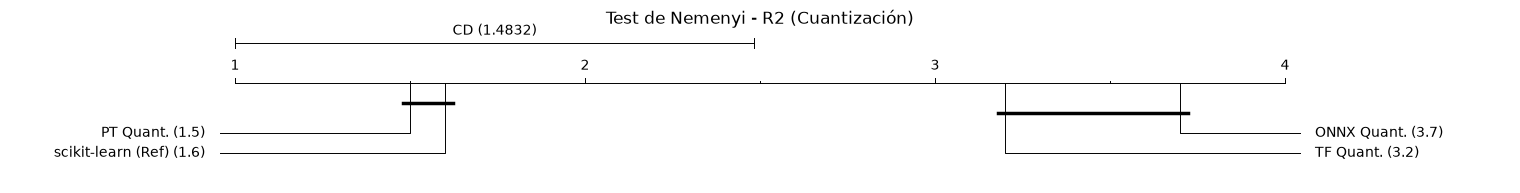
\includegraphics[width=1.0\textwidth]{phase3_quant_nemenyi_r2.png}
    \caption{Diagrama de distancia crítica de Nemenyi para los modelos de redes neuronales con cuantización en regresión según R$^2$.}
    \label{fig:nn_reg_quant_nemenyi_r2}
\end{figure}
El análisis de la capacidad predictiva confirma matemáticamente la gran disparidad de los motores. PyTorch es el
ecosistema más seguro estadísticamente para cuantizar tareas de regresión en este estudio. PyTorch se distancia
holgadamente de de TensorFlow Lite y ONNX, lo que prueba de forma concluyente que la calibración con FX Graph Mode logra
preservar la integridad de las variables continuas, mientras que el forzado estricto a tipos enteros de TensorFlow no
deja en tan buen estado la función de mapeo subyacente.\\

\begin{figure}[htbp]
    \centering
    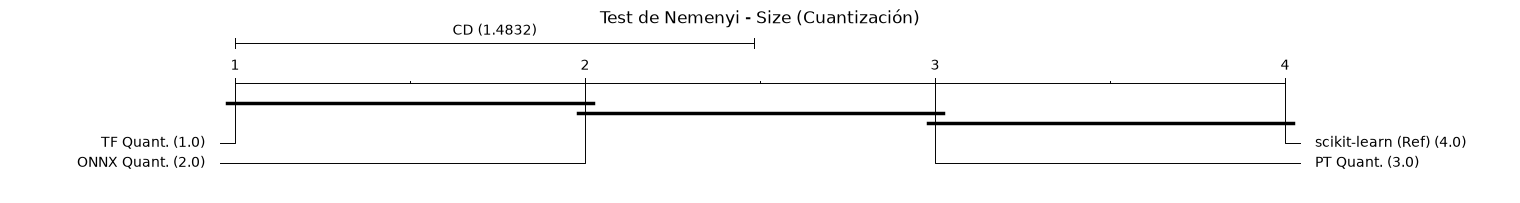
\includegraphics[width=1.0\textwidth]{phase3_reg_quant_nemenyi_size.png}
    \caption{Diagrama de distancia crítica de Nemenyi para los modelos de redes neuronales con cuantización en regresión según el tamaño en disco.}
    \label{fig:nn_reg_quant_nemenyi_size}
\end{figure}
Los tests otorgan a TensorFlow el rango de compresión perfecto. Al evaluar la distacia crítica de Nemenyi, se certifica
que el entorno de Google logra una reducción de memoria estadísticamente superior no solo frente al modelo base, sino
también frente a su rival directo, PyTorch, lo que valida matemáticamente que la serialización \path{.tflite} empaqueta
los tensores INT8 de una forma significativamente más eficiente que el formato TorchScript.\\

\begin{figure}[htbp]
    \centering
    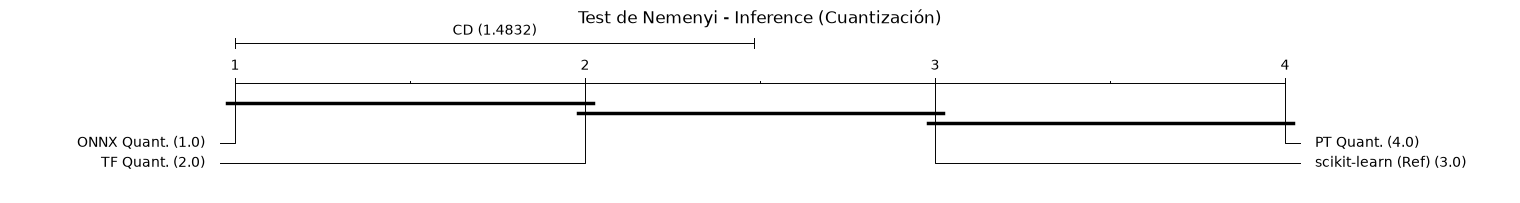
\includegraphics[width=1.0\textwidth]{phase3_reg_quant_nemenyi_inference.png}
    \caption{Diagrama de distancia crítica de Nemenyi para los modelos redes neuronales con cuantización en regresión según el tiempo de inferencia.}
    \label{fig:nn_reg_quant_nemenyi_inference}
\end{figure}
ONNX Runtime y TensorFlow Lite se consolidan como los motores de ejecución estadísticamente más rápidos, liderando la
eficiencia computacional en CPU. El contraste crítico reside en PyTorch, que queda relegado mediante el test de Nemenyi al
mismo bloque estadístico que el modelo original de Python. Esto demuestra que, si bien PyTorch es el framework que mejor
protege el coeficiente de determinación ($R^2$) al cuantizar, su runtime sigue sufriendo una penalización significativa
por la inicialización dinámica de tensores unitarios.

\subsubsection{Destilación de conocimiento}
A diferencia de las tareas de clasificación, donde la destilación extrae información de las probabilidades suavizadas
mediante el hiperparámetro de temperatura, en los problemas de regresión este concepto no es aplicable. Aquí, la red
neuronal estudiante aprende minimizando una función de pérdida combinada: el error cuadrático respecto a las
etiquetas reales y el error cuadrático respecto a las predicciones continuas emitidas por el modelo profesor. Esta fase
evalúa cómo la transferencia de este mapa de características en coma flotante impacta en el despliegue nativo.

\newpage
\subsubsection{Rendimiento predictivo (R$^2$)}
\begin{table}[htbp]
  \centering
  \small % Reduce ligeramente el tamaño de la fuente para mejorar la legibilidad
  % 'l' para la primera columna de datasets y 'X' para que las de modelos se distribuyan equitativamente
  \begin{tabularx}{\textwidth}{l *{5}{>{\centering\arraybackslash}X}}
    \hline
    \textbf{Dataset} & \textbf{PT KD} & \textbf{TF KD} \\
    \hline
    ABALONE                      & 0.56649 & 0.51496 \\
    AIR QUALITY                  & 0.89555 & 0.89106 \\
    APPLIANCES ENERGY PREDICTION & 0.70469 & 0.68603 \\
    AUTOMOBILE                   & 0.90633 & 0.89327 \\
    BIKE SHARING HOURLY          & 0.92747 & 0.93274 \\
    COMMUNITIES AND CRIME        & 0.53723 & 0.53027 \\
    OBESITY LEVELS               & 0.97919 & 0.97403 \\
    REAL ESTATE VALUATION        & 0.63307 & 0.62423 \\
    STUDENT PERFORMANCE          & 0.71700 & 0.65274 \\
    WINE QUALITY                 & 0.34048 & 0.33380 \\
    \hline
    \textbf{Media global} & \textbf{0.72075} & \textbf{0.70331} \\
    \hline
  \end{tabularx}
  \caption{R$^2$ por dataset para los modelos de redes neuronales con destilación de conocimiento en regresión.}
  \label{tab:nn_kd_r2}
\end{table}
Los resultados indican que las predicciones continuas del modelo profesor actúan como un buen mecanismo de regularización
topológica. Al guiar al estudiante, se mitiga el ruido inherente a las etiquetas originales, ofreciendo gradientes más
estables durante el entrenamiento. En PyTorch, este enriquecimiento semántico eleva el coeficiente de determinación medio
a $0.72075$, logrando superar la capacidad predictiva del modelo base original entrenado en scikit-learn ($0.71102$).
TensorFlow Lite experimenta un rendimiento ligeramente inferior ($0.70331$), pero muy superior a la caída que sufría en la
fase de cuantización pura ($0.61276$). Al operar nativamente en FP32, ambos frameworks evitan los problemas de recorte y
truncamiento de escala, permitiendo que la red estudiante retenga íntegramente las complejas fronteras de regresión
asimiladas del profesor.

\subsubsection{Huella de memoria (tamaño en disco en KB)}
\begin{table}[htbp]
  \centering
  \small % Reduce ligeramente el tamaño de la fuente para mejorar la legibilidad
  % 'l' para la primera columna de datasets y 'X' para que las de modelos se distribuyan equitativamente
  \begin{tabularx}{\textwidth}{l *{5}{>{\centering\arraybackslash}X}}
    \hline
    \textbf{Dataset} & \textbf{PT KD} & \textbf{TF KD} \\
    \hline
    ABALONE                      & 7.39160  & 5.42578  \\
    AIR QUALITY                  & 12.76855 & 10.88672 \\
    APPLIANCES ENERGY PREDICTION & 10.39551 & 8.51172  \\
    AUTOMOBILE                   & 15.39551 & 13.51172 \\
    BIKE SHARING HOURLY          & 7.64551  & 5.77344  \\
    COMMUNITIES AND CRIME        & 18.64551 & 16.77344 \\
    OBESITY LEVELS               & 9.52051  & 7.64844  \\
    REAL ESTATE VALUATION        & 6.89551  & 5.02344  \\
    STUDENT PERFORMANCE          & 13.39551 & 11.52344 \\
    WINE QUALITY                 & 7.52051  & 5.64844  \\
    \hline
    \textbf{Media global} & \textbf{10.95742} & \textbf{9.07266} \\
    \hline
  \end{tabularx}
  \caption{Tamaño en disco por dataset para los modelos de redes neuronales con destilación de conocimiento en regresión.}
  \label{tab:nn_kd_reg_size}
\end{table}
Dado que la destilación no altera la arquitectura final del modelo en producción, el tamaño del artefacto depende
exclusivamente del formato de serialización en FP32. TensorFlow Lite vuelve a imponer su superioridad arquitectónica,
promediando $9.07$ KB frente a los $10.95$ KB del formato TorchScript de PyTorch. Es imperativo destacar que, incluso sin
aplicar técnicas de reducción de precisión numérica, el simple hecho de compilar el grafo computacional en estos lenguajes
nativos ya supone una drástica optimización frente a los $38.56$ KB que ocupa el modelo equivalente en Python, logrando
reducir la huella de memoria en más de un $70\%$.

\subsubsection{Eficiencia operativa (ms), resultados globales y comparativa}
\begin{table}[htbp]
  \centering
  \begin{tabularx}{\textwidth}{lXccc}
    \hline
    \textbf{Framework / Configuración} & \textbf{R$^2$} & \textbf{Inferencia (ms)} & \textbf{Tamaño (KB)} \\
    \hline
    \textbf{scikit-learn}     & 0.71102  & 0.157 & 38.56562 \\
    \hline
    \textbf{PT KD}            & 0.72075 & 0.188 & 10.95742  \\
    \hline
    \textbf{TF KD}            & 0.70331 & 0.12 & 9.07266    \\
    \hline
  \end{tabularx}
  \caption{Comparativa de rendimiento y coste de redes neuronales con destilación de conocimiento en regresión.}
  \label{tab:nn_kd_reg_resumen}
\end{table}
La síntesis de resultados manifiesta que la destilación de conocimiento en regresión es una estrategia sin contrapartidas
técnicas.
\begin{itemize}
  \item La configuración con PyTorch demuestra que un modelo ligero puede superar su propio límite teórico de aprendizaje
  si es guiado por un ensamblado paramétrico superior, sin requerir la adición de nuevas capas o neuronas.
  \item Al operar con tensores en coma flotante y carecer del \textit{overhead} de las operaciones de cuantización, los
  motores de C++ subyacentes alcanzan su máxima eficiencia. TensorFlow supera los 0.157 ms de scikit-learn, mientras que
  PyTorch sigue quedándose algo más atascado, aunque sigue siendo una latencia asumible para microcontroladores.
\end{itemize}

\begin{figure}[htbp]
    \centering
    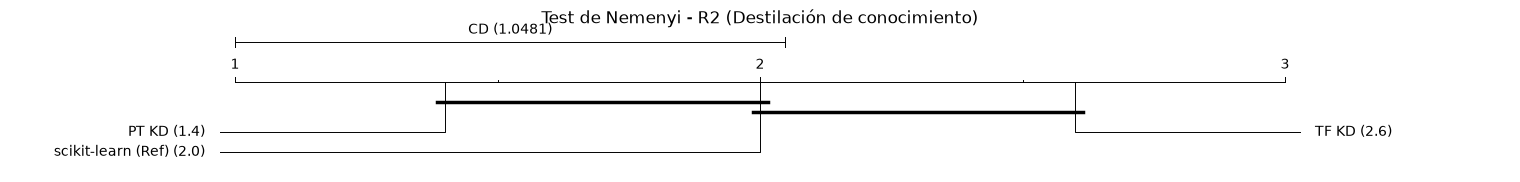
\includegraphics[width=1.0\textwidth]{phase4_distill_nemenyi_r2.png}
    \caption{Diagrama de distancia crítica de Nemenyi para los modelos redes neuronales con destilación de conocimiento en regresión según R$^2$.}
    \label{fig:nn_reg_kd_nemenyi_r2}
\end{figure}
El test de Friedman revela divergencias significativas en las distribuciones en lo que a R$^2$ respecta. Observando el
diagrama de distancia crítica, es PyTorch el framework logra coronarse como vencedor en esta métrica, distanciándose
estadísticamente de TensorFlow. Aunque su separación con el modelo base no logre superar el umbral de significancia, se
consolida como mejor opción, validando las observaciones anteriores.\\

\newpage
\begin{figure}[htbp]
    \centering
    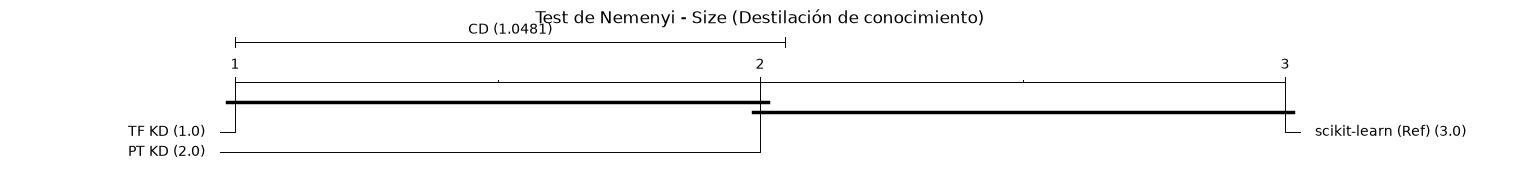
\includegraphics[width=1.0\textwidth]{phase4_reg_distill_nemenyi_size.png}
    \caption{Diagrama de distancia crítica de Nemenyi para los modelos redes neuronales con destilación de conocimiento en regresión según el tamaño en disco.}
    \label{fig:nn_reg_kd_nemenyi_size}
\end{figure}
La evaluación de la compresión espacial ratifica los patrones de diseño subyacentes de los frameworks. TensorFlow vuelve
a colocarse como el entorno que consigue separarse de forma estadística del ineficiente modelo base de Python, quedando
PyTorch en una zona de transición entre ambos. Esto subraya nuevamente que TensorFlow gestiona la serialización con una
eficiencia de empaquetado notablemente superior a TorchScript.

\begin{figure}[htbp]
    \centering
    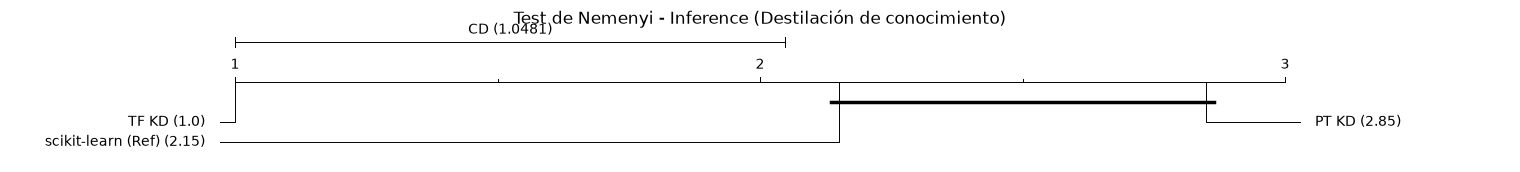
\includegraphics[width=1.0\textwidth]{phase4_reg_distill_nemenyi_inference.png}
    \caption{Diagrama de distancia crítica de Nemenyi para los modelos redes neuronales con destilación de conocimiento en regresión según el tiempo de inferencia.}
    \label{fig:nn_reg_kd_nemenyi_inference}
\end{figure}
Las latencias exponen una divergencia drástica en la optimización de los motores computacionales al operar sobre grafos de
regresión en FP32. Según el diagrama de distancia crítica de Nemenyi, TensorFlow se aísla por completo como el motor más
rápido, superando la barrera crítica de Nemenyi tanto frente al modelo base como frente a PyTorch. El intérprete C++ de
TensorFlow Lite despliega todo su potencial, logrando una aceleración estadísticamente significativa respecto a sus
competidores. Por el contrario, PyTorch queda agrupado en el mismo bloque estadístico que scikit-learn, lo que evidencia
que el invocador JIT de TorchScript sigue arrastrando una sobrecarga al procesar inferencias de regresión.

\subsubsection{Cuantización + destilación de conocimiento}
De forma análoga al trabajo realizado en clasificación, se evalúa la utilización conjunta de cuantización y destilación de
conocimiento. Igualmente, se tiene como propósito resolver si la transferencia de fronteras entre profesor y estudiante es
suficiente para amortiguar pérdida en rendimiento predictivo al truncar los tensores a 8 bits durante la cuantización.

\newpage
\subsubsection{Rendimiento predictivo (R$^2$)}
\begin{table}[htbp]
  \centering
  \small % Reduce ligeramente el tamaño de la fuente para mejorar la legibilidad
  % 'l' para la primera columna de datasets y 'X' para que las de modelos se distribuyan equitativamente
  \begin{tabularx}{\textwidth}{l *{5}{>{\centering\arraybackslash}X}}
    \hline
    \textbf{Dataset} & \textbf{PT quant. KD} & \textbf{TF quant. KD} \\
    \hline
    ABALONE                      & 0.54247 & 0.45177 \\
    AIR QUALITY                  & 0.89438 & 0.86956 \\
    APPLIANCES ENERGY PREDICTION & 0.70094 & 0.66929 \\
    AUTOMOBILE                   & 0.90688 & 0.88851 \\
    BIKE SHARING HOURLY          & 0.91938 & 0.34829 \\
    COMMUNITIES AND CRIME        & 0.53709 & 0.54016 \\
    OBESITY LEVELS               & 0.96989 & 0.92779 \\
    REAL ESTATE VALUATION        & 0.63293 & 0.58723 \\
    STUDENT PERFORMANCE          & 0.72508 & 0.63761 \\
    WINE QUALITY                 & 0.33464 & 0.33449 \\
    \hline
    \textbf{Media global} & \textbf{0.71637} & \textbf{0.62547} \\
    \hline
  \end{tabularx}
  \caption{R$^2$ por dataset para los modelos de redes neuronales con cuantización y destilación de conocimiento en regresión.}
  \label{tab:nn_quant_kd_r2}
\end{table}
Los resultados sugieren que el impacto de la aplicación híbrida depende de la robustez del calibrador de cuantización de
cada framework. En TensorFlow, la inyección del conocimiento del profesor actúa como un mecanismo de mitigación parcial.
La variante híbrida asciende a un $R^2$ global de 0.62547, superando el 0.61276 obtenido antes mediante cuantización pura.
Sin embargo, el enriquecimiento del mapa de características durante el entrenamiento no puede sortear la limitación física
del motor de TFLite, que produce un recorte importante al realizar la cuantización. Por su parte, la versión de PyTorch
vuelve a vencer a su rival, logrando un sobresaliente $R^2$ de 0.71637 que también supera al modelo base original de
scikit-learn (0.71102).

\subsubsection{Huella de memoria (tamaño en disco en KB)}
\begin{table}[htbp]
  \centering
  \small % Reduce ligeramente el tamaño de la fuente para mejorar la legibilidad
  % 'l' para la primera columna de datasets y 'X' para que las de modelos se distribuyan equitativamente
  \begin{tabularx}{\textwidth}{l *{5}{>{\centering\arraybackslash}X}}
    \hline
    \textbf{Dataset} & \textbf{PT quant. KD} & \textbf{TF quant. KD} \\
    \hline
    ABALONE                      & 8.56543  & 4.36719 \\
    AIR QUALITY                  & 9.87988  & 5.80469 \\
    APPLIANCES ENERGY PREDICTION & 9.31934  & 5.21094 \\
    AUTOMOBILE                   & 10.56934 & 6.46094 \\
    BIKE SHARING HOURLY          & 8.63184  & 4.52344 \\
    COMMUNITIES AND CRIME        & 11.38184 & 7.27344 \\
    OBESITY LEVELS               & 9.06934  & 4.99219 \\
    REAL ESTATE VALUATION        & 8.44434  & 4.33594 \\
    STUDENT PERFORMANCE          & 10.06934 & 5.96094 \\
    WINE QUALITY                 & 8.56934  & 4.49219 \\
    \hline
    \textbf{Media global} & \textbf{9.45000} & \textbf{5.34219} \\
    \hline
  \end{tabularx}
  \caption{Tamaño en disco por dataset para los modelos de redes neuronales con cuantización y destilación de conocimiento en regresión.}
  \label{tab:nn_quant_kd_reg_size}
\end{table}
Al igual que ocurría en clasificación, Las huellas de memoria de las variantes híbridas son matemáticamente idénticas a
las generadas en la fase de cuantización pura en ambos frameworks. Cuando finaliza la convergencia guiada por el profesor,
el grafo paramétrico complejo se descarta, permitiendo que los sistemas hereden el conocimiento avanzado en un archivo
binario cuantizado que ocupa menos de 10 KB.

\subsubsection{Resultados globales y comparativa}
Dando un vistazo general a los valores de R$^2$, tamaño y latencia, puede confirmarse que la complejidad del entrenamiento
no penaliza el despliegue.
\begin{itemize}
  \item Al operar exclusivamente sobre tensores INT8, los tiempos de inferencia alcanzan el orden de los
  sub-microsegundos en ambos ecosistemas. Imitando el comportamiento que se observaba en clasificación, el uso de la
  destilación de conocimiento no introduce sobrecarga adicional, de modo que los tiempos se mantienen en el mismo rango
  que los obtenidos en la fase de cuantización pura.
  \item Lo mismo ocurre con el tamaño en disco, que permanece inalterado respecto a la fase de cuantización pura. La
  destilación de conocimiento no añade complejidad al grafo final, de modo que el artefacto resultante sigue teniendo un
  peso inferior a 10 KB en todos los casos, una reducción del $\sim 75.5\%$ frente al modelo en Python.
  \item Un comportamiento a destacar es el de la red de PyTorch que, aunque el valor de R$^2$ que alcanza combinando ambas
  técnicas sigue siendo superior al de TensorFlow con esta misma configuración, resulta ser marginalmente inferior al que
  se consigue únicamente con cuantización. Un posible motivo es que su algoritmo de calibración ya realiza un buen mapeo
  FP32-INT8, de modo que la destilación queda relegada como una función regularizadora.
\end{itemize}

\subsubsection{Eficiencia operativa (ms), resultados globales y comparativa en PyTorch}
\begin{table}[htbp]
  \centering
  \begin{tabularx}{\textwidth}{lXccc}
    \hline
    \textbf{Framework / Configuración} & \textbf{R$^2$} & \textbf{Inferencia (ms)} & \textbf{Tamaño (KB)} \\
    \hline
    \textbf{scikit-learn}     & 0.71102  & 0.157 & 38.56562 \\
    \hline
    \textbf{PT quant.}        & 0.71539 & 0.229 & 9.44961   \\
    \textbf{PT KD}            & 0.72075 & 0.188 & 10.95742  \\
    \textbf{PT quant. $+$ KD} & 0.71637 & 0.228 & 9.45000   \\
    \hline
  \end{tabularx}
  \caption{Comparativa de rendimiento y coste de redes neuronales en PyTorch con cuantización y destilación de conocimiento en regresión.}
  \label{tab:pytorch_quant_kd_reg_resumen}
\end{table}

\newpage
\begin{figure}[htbp]
    \centering
    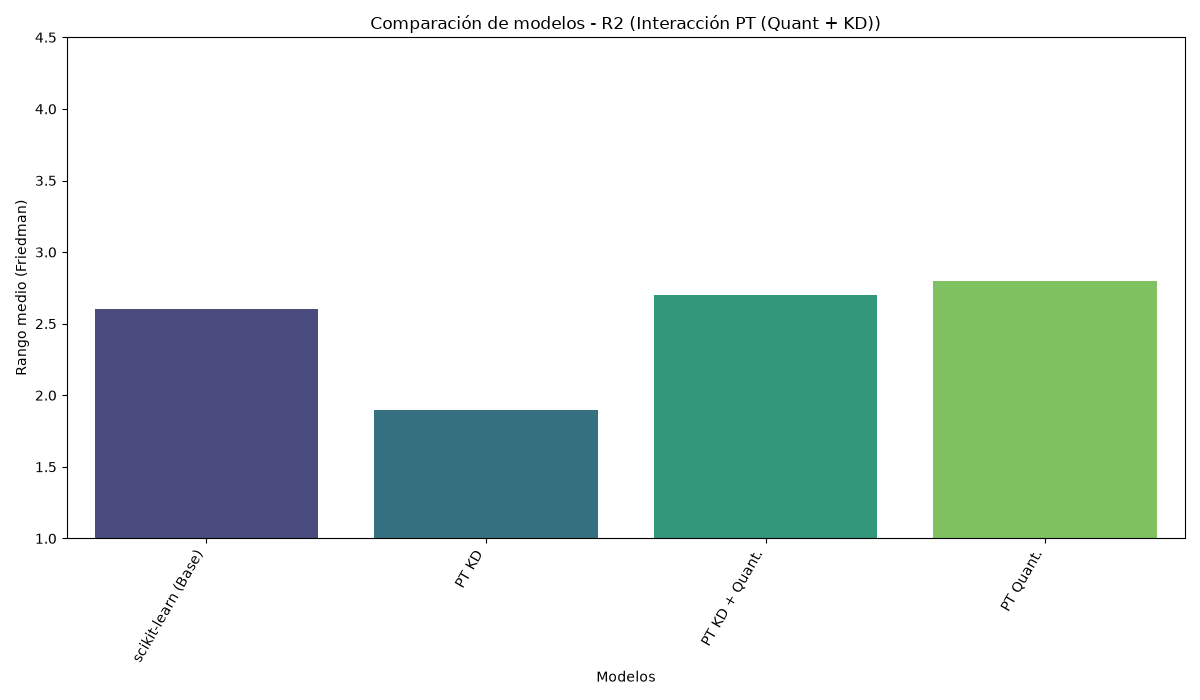
\includegraphics[width=1.0\textwidth]{phase5_pytorch_average_ranks_r2.png}
    \caption{Rangos medios de los modelos PyTorch con cuantización y destilación de conocimiento en regresión según R$^2$.}
    \label{fig:pt_quant_kd_ranks_r2}
\end{figure}
En PyTorch, el test de Friedman determina un $p$-valor de 0.3916, lo que obliga a mantener la hipótesis nula para R$^2$.
Atendiendo a los rangos medios, la variante híbrida convive en el mismo espacio estadístico que el modelo original de
scikit-learn y el modelo cuantizado puro, seguidos por la configuración de destilación de conocimiento. Esto demuestra
la robustez del ecosistema de PyTorch, que no se ve alterado de forma significativa por la adición de técnicas de
optimización, manteiéndose en la línea de su comportamiento frente a problemas de clasificación.\\

\begin{figure}[htbp]
    \centering
    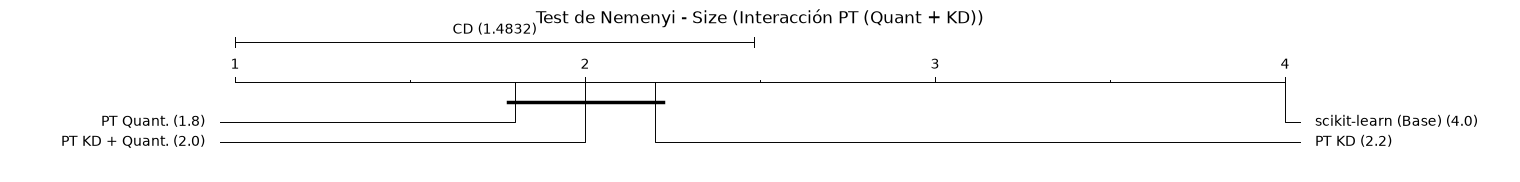
\includegraphics[width=1.0\textwidth]{phase5_reg_pytorch_nemenyi_size.png}
    \caption{Diagrama de distancia crítica de Nemenyi para los modelos PyTorch con cuantización y destilación de conocimiento en regresión según el tamaño en disco.}
    \label{fig:pt_reg_quant_kd_nemenyi_size}
\end{figure}
El almacenamiento físico sí rechaza la hipótesis nula, con $p < 0.001$. Haciendo al modelo de scikit-learn
a un lado, que sí se distancia claramente de las arquitecturas nativas con técnicas de optimización, las variaciones de
combinaciones de estas no muestran diferencias significativas, dando prueba matématica de que se mantiene lo ya verificado
en clasificación: la destilación es una estrategia transitoria que no supone ninguna penalización en el tamaño final del
modelo.\\

\newpage
\begin{figure}[htbp]
    \centering
    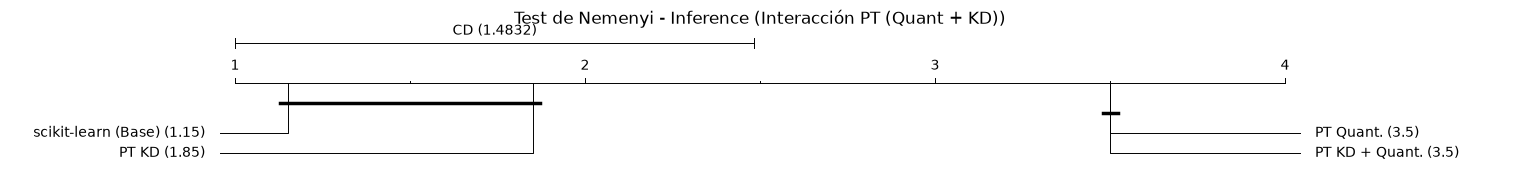
\includegraphics[width=1.0\textwidth]{phase5_reg_pytorch_nemenyi_inference.png}
    \caption{Diagrama de distancia crítica de Nemenyi para los modelos PyTorch con cuantización y destilación de conocimiento en regresión según el tiempo de inferencia.}
    \label{fig:pt_reg_quant_kd_nemenyi_inference}
\end{figure}
El test de Nemenyi confirma el cuello de botella de PyTorch en CPU. Las variantes cuantizadas empatan en el último rango,
siendo estadísticamente más lentas que el modelo base de scikit-learn en FP32 que, aunque no de forma significativa, llega
a superar a la arquitectura que utiliza destilación de conocimiento.

\subsubsection{Eficiencia operativa (ms), resultados globales y comparativa en TensorFlow}
\begin{table}[htbp]
  \centering
  \begin{tabularx}{\textwidth}{lXccc}
    \hline
    \textbf{Framework / Configuración} & \textbf{R$^2$} & \textbf{Inferencia (ms)} & \textbf{Tamaño (KB)} \\
    \hline
    \textbf{scikit-learn}     & 0.71102  & 0.157 & 38.56562 \\
    \hline
    \textbf{TF quant.}        & 0.61276 & 0.13 & 5.33906    \\
    \textbf{TF KD}            & 0.70331 & 0.12 & 9.07266    \\
    \textbf{TF quant. $+$ KD} & 0.62547 & 0.13 & 5.34219    \\
    \hline
  \end{tabularx}
  \caption{Comparativa de rendimiento y coste de redes neuronales en TensorFlow con cuantización y destilación de conocimiento en regresión.}
  \label{tab:tflite_quant_kd_reg_resumen}
\end{table}

\begin{figure}[htbp]
    \centering
    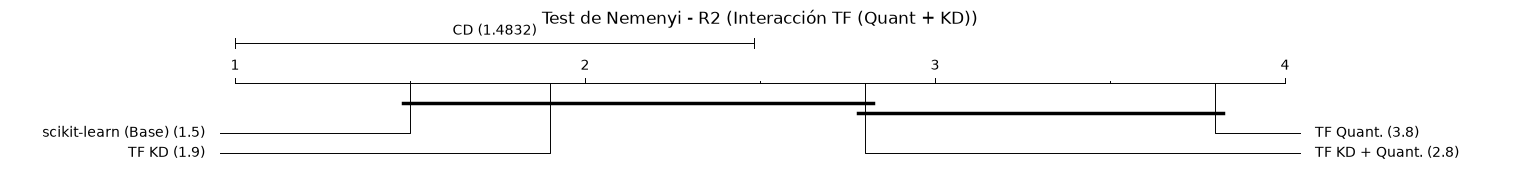
\includegraphics[width=1.0\textwidth]{phase6_tensorflow_nemenyi_r2.png}
    \caption{Diagrama de distancia crítica de Nemenyi para los modelos TensorFlow con cuantización y destilación de conocimiento en regresión según R$^2$.}
    \label{fig:tf_quant_kd_nemenyi_r2}
\end{figure}
El análisis de R$^2$ para TensorFlow sí muestra diferencias significativas, siendo revelador el impacto de la destilación.
El modelo con cuantización pura obtiene el peor rango y se distancia de la implementación base. Sin embargo, al integrar
la destilación de conocimiento, el modelo híbrido logra entrar en el mismo bloque estadístico que el modelo original. Esto
no hace más que probar que la inyección del conocimiento del profesor consigue rescatar al modelo de TensorFlow, si bien
lo hace por la mínima, aunque la alternativa con únicamente destilación de conocimiento logra un rango superior.

\newpage
\begin{figure}[htbp]
    \centering
    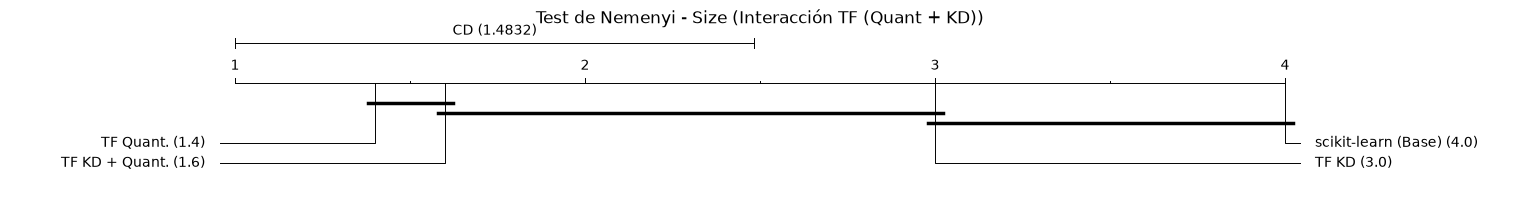
\includegraphics[width=1.0\textwidth]{phase6_reg_tensorflow_nemenyi_size.png}
    \caption{Diagrama de distancia crítica de Nemenyi para los modelos TensorFlow con cuantización y destilación de conocimiento en regresión según el tamaño en disco.}
    \label{fig:tf_reg_quant_kd_nemenyi_size}
\end{figure}
Las conclusiones que pueden obtenerse en el caso de TensorFlow son equivalentes a las de PyTorch. Las configuraciones
cuantizadas siguen siendo las superiores, siendo nulo el impacto de la destilación de conocimiento en el peso del modelo.

\begin{figure}[htbp]
    \centering
    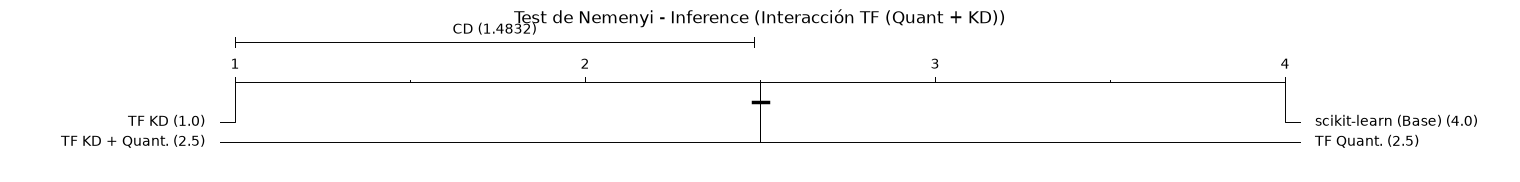
\includegraphics[width=1.0\textwidth]{phase6_reg_tensorflow_nemenyi_inference.png}
    \caption{Diagrama de distancia crítica de Nemenyi para los modelos TensorFlow con cuantización y destilación de conocimiento en regresión según el tiempo de inferencia.}
    \label{fig:tf_reg_quant_kd_nemenyi_inference}
\end{figure}
Para el tiempo de inferencia, también se obtienen diferencia significativas. Sin embargo, en contraposición a PyTorch, los
modelos de TensorFlow sí consiguen separarse de forma estadísticamente significativa del modelo inicial de scikit-learn.

\subsection{MLP}
Como punto final de este bloque de presentación de resultados y tests estadísticos, se ha decicido dedicar un apartado
exclusivamente al perceptrón multicapa, ya que es la única arquitectura que se despliega en los cuatro frameworks y que,
por tanto, permite una comparativa directa de rendimiento y coste entre todos ellos. Esta síntesis aglomera todas las
estrategias de optimización evluadas, ofreciendo una perspectiva panorámica de la eficiencia de cada motor de ejecución y
de la capacidad predictiva de cada configuración.\\

\subsubsection{Clasificación}
El modelo base instanciado en scikit-learn establece el punto de partida. Cuenta con un rendimiento predictivo sólido
(0.88738), pero su huella de memoria es masiva (126.65 KB) en comparacion con los modelos optimizados, y además tiene una
dependencia absoluta del entorno de ejecución de Python, lo que lo inhabilita para microcontroladores o sistemas embebidos.
A partir de este límite, las técnicas de compresión trazan trayectorias distintas.
\newpage
\begin{table}[htbp]
  \centering
  \begin{tabularx}{\textwidth}{lXccc}
    \hline
    \textbf{Framework / Configuración} & \textbf{F1} & \textbf{Inferencia (ms)} & \textbf{Tamaño (KB)} \\
    \hline
    \textbf{scikit-learn}     & 0.88738 & 0.231 & 126.65029 \\
    \hline
    \textbf{ONNX quant.}      & 0.81938 & 0.023 & 14.34600  \\
    \hline
    \textbf{PT quant.}        & 0.88395 & 0.174 & 13.06836  \\
    \textbf{PT T1}            & 0.89003 & 0.137 & 25.18242  \\
    \textbf{PT T2}            & 0.89124 & 0.136 & 25.18242  \\
    \textbf{PT quant. $+$ T1} & 0.88709 & 0.172 & 13.06875  \\
    \textbf{PT quant. $+$ T2} & 0.88871 & 0.174 & 13.06875  \\
    \hline
    \textbf{TF quant.}        & 0.87741 & 0.081 & 9.08594   \\
    \textbf{TF T1}            & 0.88725 & 0.071 & 23.31563  \\
    \textbf{TF T2}            & 0.88935 & 0.071 & 23.31563  \\
    \textbf{TF quant. $+$ T1} & 0.88040 & 0.081 & 9.08984   \\
    \textbf{TF quant. $+$ T2} & 0.88292 & 0.081 & 9.08984   \\
    \hline
  \end{tabularx}
  \caption{Comparativa de rendimiento y coste del MLP en los distintos frameworks en clasificación.}
  \label{tab:mlp_clas_resumen}
\end{table}
La exportación agnóstica mediante ONNX cuantizado expone un riesgo al aplicar transformaciones topológicas agresivas sin
una calibración nativa profunda. Si bien su motor en C minimizado pulveriza todos los registros de latencia
(0.023 ms), el coste es inasumible desde el rigor analítico: el F1-score colapsa a 0.81938. Al existir mejores opciones
con latencias poco mayores, esta degradación invalida a ONNX como opción de despliegue confiable en este contexto,
evidenciando que el mapeo a INT8, junto a la poda de pesos aplicada, empeoran los límites de decisión espaciales del MLP
más de lo que lo hacen los frameworks nativos.\\

Cuando el objetivo del diseño es maximizar la capacidad de generalización sin restricciones extremas de hardware, el
entorno de PyTorch se muestra como el estándar indiscutible. Las configuraciones con destilación de conocimiento logran
superar el techo predictivo del modelo base, alcanzando un F1-score sobresaliente de 0.89124 en el caso de $T=2$. Esto
ratifica que la transferencia desde un ensamblado profundo, permite que el MLP retenga una riqueza probabilística aún
mayor.\\

Para escenarios donde cada kilobyte cuenta, TensorFlow Lite demuestra una arquitectura de serialización insuperable. Su
configuración híbrida óptima, también con $T=2$, encapsula una capacidad predictiva de 0.88292 en un archivo de apenas
9.08 KB. Este hito representa una compresión superior al $92\%$ respecto al modelo original en Python. A nivel operativo,
TFLite logra mantener una latencia en niveles muy bajos, evitando el cuello de botella que sufre PyTorch al decuantizar/
cuantizar activaciones al vuelo.\\

\newpage
\begin{figure}[htbp]
    \centering
    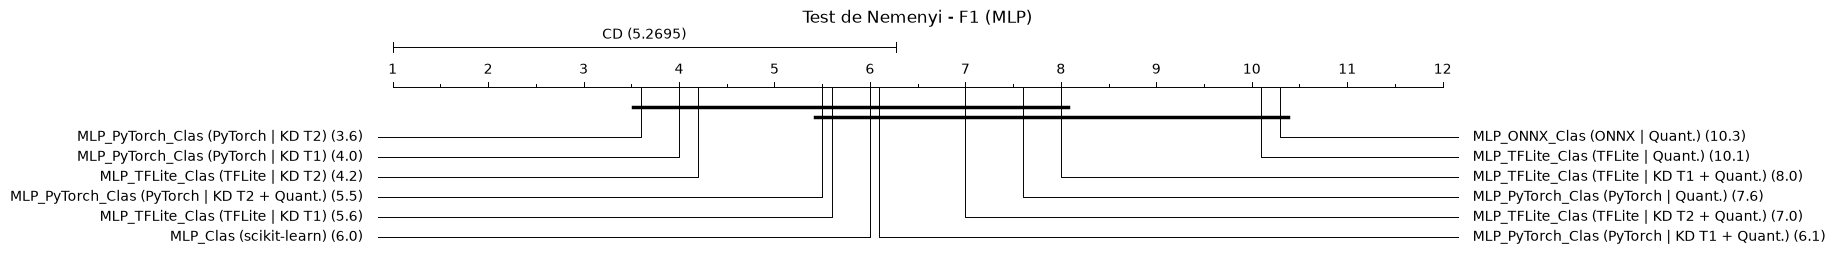
\includegraphics[width=1.0\textwidth]{mlp_nemenyi_f1.png}
    \caption{Diagrama de distancia crítica de Nemenyi para los MLP en clasificación según F1-score.}
    \label{fig:mlp_nemenyi_f1}
\end{figure}
El test de Nemenyi certifica estadísticamente las carencias de los procesos de cuantización frente a los métodos de
enriquecimiento del conocimiento. Las arquitecturas que implementan la destilación de conocimiento, en especial las de
PyTorch, se colocan como las líderes y se separan de forma significativa del resto de configuraciones, corroborando el
análisis previo. Al mismo tiempo, también se confirma que la adición de cuantización al modelo supone una pérdida de
capacidad predictiva, lo que da soporte a la hipótesis de que la reducción de precisión numérica degrada las fronteras
de decisión a cambio de una mejora en la huella de memoria.\\

\begin{figure}[htbp]
    \centering
    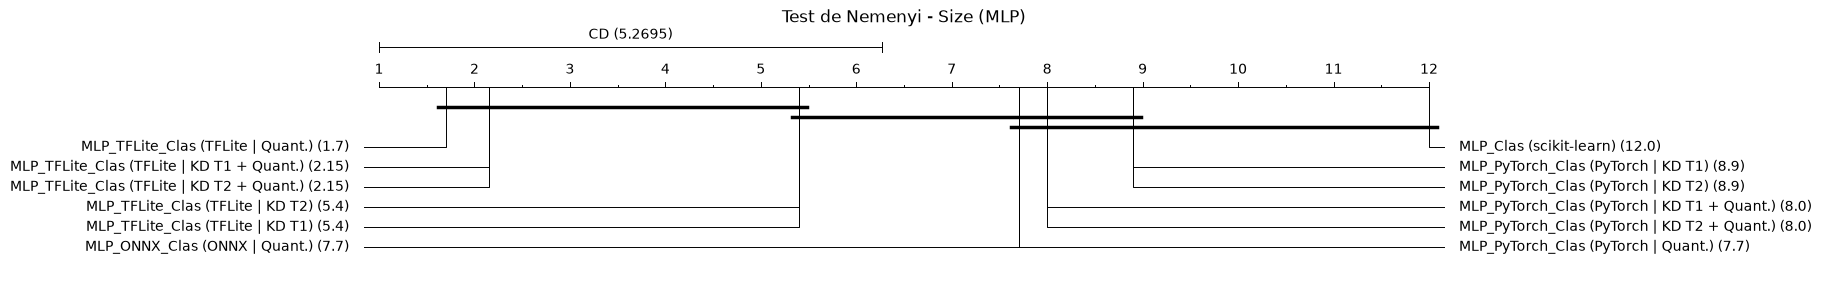
\includegraphics[width=1.0\textwidth]{mlp_nemenyi_size.png}
    \caption{Diagrama de distancia crítica de Nemenyi para los MLP en clasificación según el tamaño en disco.}
    \label{fig:mlp_nemenyi_size}
\end{figure}
La optimización del almacenamiento constata el dominio de las estructuras \textit{FlatBuffers} de TensorFlow Lite. A
través del diagrama de distancia crítica, se prueba que, especialmente sus configuraciones cuantizadas, alcazan una
separación estadísticamente significativa frente a las topologías equivalentes de PyTorch y la versión exportada a ONNX,
además de, por supuesto, frente al pesado modelo base. Esto consolida a TensorFlow como el ecosistema que garantiza de
forma matemática el mayor grado de compresión para redes neuronales en el estudio.\\

\begin{figure}[htbp]
    \centering
    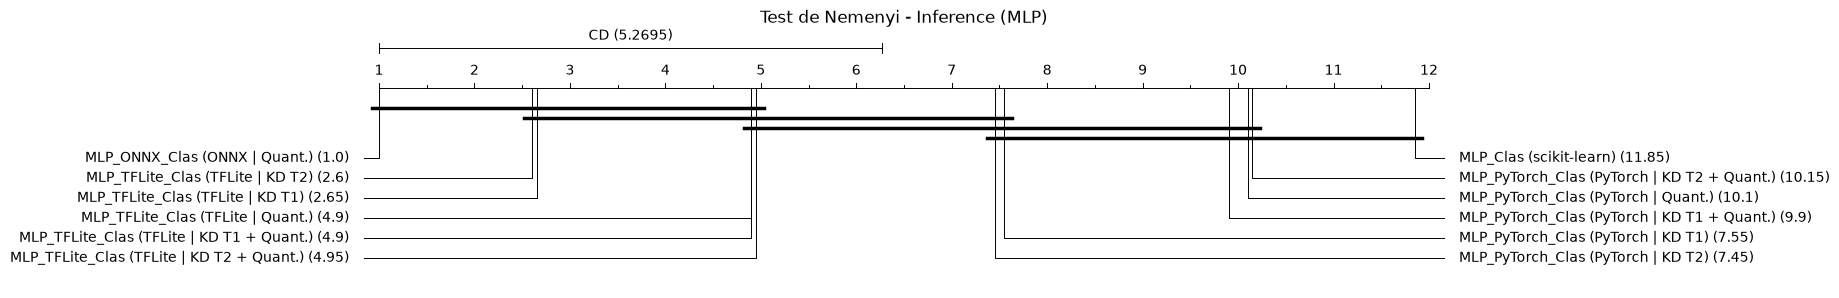
\includegraphics[width=1.0\textwidth]{mlp_nemenyi_inference.png}
    \caption{Diagrama de distancia crítica de Nemenyi para los MLP en clasificación según el tiempo de inferencia.}
    \label{fig:mlp_nemenyi_inference}
\end{figure}
El análisis de las latencias permite exponer algunas conclusiones interesantes. En primer lugar, verifica a ONNX como el
motor más veloz, seguido de cerca por el bloque de TensorFlow Lite, sin que exista una diferencia significativa entre
ellos. Asimismo, revela y ratifica el defecto de PyTorch. Las configuraciones cuantizadas, seguidas por la destilación,
se desploman a los rangos más bajos, quedando encapsuladas en el mismo grupo estadístico que el modelo de scikit-learn.
La estadística dictamina que el invocador de PyTorch, al penalizar cada inferencia individual con decuantizaciones
dinámicas, destruye por completo las teóricas ventajas de velocidad de los tensores INT8, marginándolo frente a la
probada eficiencia de TensorFlow Lite y ONNX Runtime.\\

Tras este estudio de las arquitecturas MLP disponibles en clasificación y puestos a seleccionar un framework y
alternativa, esta elección no puede hacerse de forma axiomática, sino que depende directamtente de las especificaciones
de la plataforma de destino y el objetivo a priorizar.
\begin{itemize}
  \item \textbf{Prioridad en la generalización predictiva}. Quedarse con en el entorno de PyTorch sería la opción más
  sensata, e idealmente con la configuración de destilación de conocimiento pura y $T=2$. Es la arquitectura que ofrece
  el mayor F1-score absoluto, teniendo además un tamaño competitivo. Sin embargo, presenta una desventaja en el tiempo
  de inferencia, que es algo superior al de otras alternativas.
  \item \textbf{Prioridad en el almacenamiento y la latencia equilibrada}. Si el microcontrolador de destino posee
  limitaciones extremas, se requiere un tiempo de respuesta aún más instantáneo y la aplicación puede tolerar un ligero
  margen de error, la aproximación híbrida de TensorFlow Lite con cuantización y destilación de conocimiento en $T=2$ es
  el punto de equilibrio global. Recupera gran parte de la precisión perdida por el truncamiento a INT8, ocupa menos de
  10 KB y garantiza inferencias sobresalientemente rápidas.
\end{itemize}

\subsubsection{Regresión}
\begin{table}[htbp]
  \centering
  \begin{tabularx}{\textwidth}{lXccc}
    \hline
    \textbf{Framework / Configuración} & \textbf{R$^2$} & \textbf{Inferencia (ms)} & \textbf{Tamaño (KB)} \\
    \hline
    \textbf{scikit-learn}     & 0.71102  & 0.157 & 38.56562 \\
    \hline
    \textbf{ONNX quant.}      & -4.90574 & 0.02  & 8.56172  \\
    \hline
    \textbf{PT quant.}        & 0.71539  & 0.229 & 9.44961  \\
    \textbf{PT KD}            & 0.72075  & 0.188 & 10.95742 \\
    \textbf{PT quant. $+$ KD} & 0.71637  & 0.228 & 9.45000  \\
    \hline
    \textbf{TF quant.}        & 0.61276  & 0.13  & 5.33906  \\
    \textbf{TF KD}            & 0.70331  & 0.12  & 9.07266  \\
    \textbf{TF quant. $+$ KD} & 0.62547  & 0.13  & 5.34219  \\
    \hline
  \end{tabularx}
  \caption{Comparativa de rendimiento y coste del MLP en los distintos frameworks en regresión.}
  \label{tab:mlp_reg_resumen}
\end{table}
El modelo original desplegado mediante scikit-learn establece un coeficiente de determinación ($R^2$) de referencia de
0.71102. Si bien su latencia es extraordinariamente baja para la CPU empleada (0.157 ms), su huella de
memoria y su dependencia del intérprete de Python impulsan la necesidad de explorar arquitecturas orientadas a la
computación en el borde.\\

Volvemos a observar el fenómeno ocurrido con ONNX. Al aplicar una política de truncamiento no nativa sobre el grafo,
junto con la poda de pesos, el coeficiente R$^2$ se hunde hasta hacer al modelo inviable. Aunque logra un tamaño
muy compacto y latencias excelentes, sus predicciones son inaceptables como un conjunto. Por tanto, podemos deducir que,
en tareas de regresión, la cuantización sin un calibrador profundo que proteja la escala de la capa de salida destruye
la función de mapeo continuo.\\

Frente a la fragilidad de ONNX, el framework de PyTorch demuestra una solvencia técnica excepcional en el dominio
continuo. Todas sus configuraciones consiguen retener o incluso superar el rendimiento predictivo original del modelo
base. La configuración con destilación de conocimiento y $T=2$ alcanza el pico predictivo de todo el estudio en
regresión ($R^2 = 0.72075$), confirmando que el mapa de características del profesor actúa como un poderoso
regularizador. En cuanto a la cuantización, el calibrador FX Graph Mode de PyTorch demuestra el que mejor mapea el
espacio FP32 a INT8 sin saturar los valores extremos, manteniendo un tamaño excelente y unas latencias por debajo del
milisegundo altamente competitivas.\\

En el extremo opuesto del espectro, TensorFlow Lite sacrifica parte de la precisión predictiva en aras de lograr la
máxima eficiencia de hardware posible. Las configuraciones apoyadas en cuantización marcan el récord absoluto de
compresión con un tamaño de 5.34 KB, una reducción superior al $86\%$ frente al modelo original, y una de las
inferencias más veloces de todo el conjunto, de 0.13 ms, junto a ONNX. No obstante, la rígida política de conversión a
\path{tf.int8} pasa factura al rango dinámico, reduciendo el $R^2$ a por debajo del obtenido en la línea base, debido al
efecto de \textit{clipping} en conjuntos de datos con alta varianza. Para evitar esta caída, la variante con destilación
pura, en coma flotante, se presenta como un excelente término medio: recupera el $R^2$ hasta 0.70331, y mantiene un peso
de apenas 9.07 KB, dejando atrás la eficiencia del modelo base en Python.\\

\begin{figure}[htbp]
    \centering
    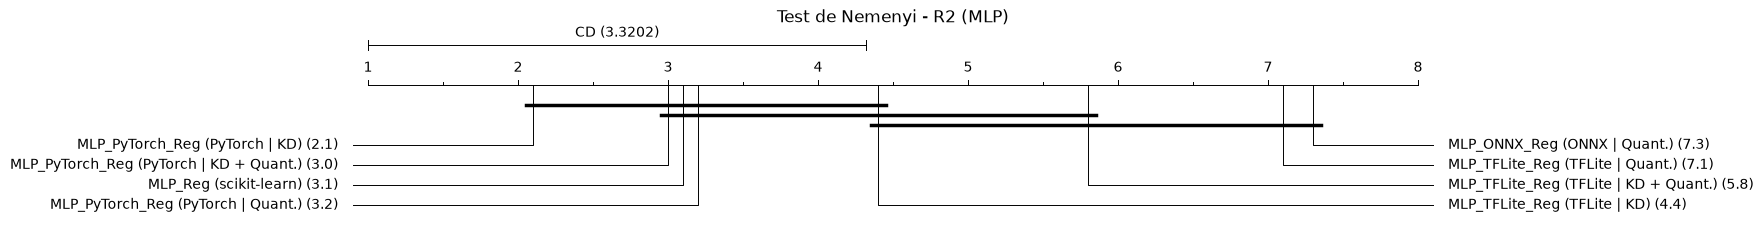
\includegraphics[width=1.0\textwidth]{mlp_nemenyi_r2.png}
    \caption{Diagrama de distancia crítica de Nemenyi para los MLP en clasificación según $R^2$.}
    \label{fig:mlp_nemenyi_r2}
\end{figure}
Los tests estadísticos sobre el rendimiento predictivo confirman la superioridad de las configuraciones de PyTorch
frente al resto de frameworks. Observando un comportamiento similar al de clasificación, las arquitecturas con
destilación de conocimiento consiguen mejores resultados, siendo al mismo tiempo esta técnica capaz de amortiguar la
pérdida de precisión que introduce la cuantización. Se confirma el fallo que comete TensorFlow con el recorte al
realizar la cuantización, que le hace perder capacidad predictiva frente al modelo base.\\

\newpage
\begin{figure}[htbp]
    \centering
    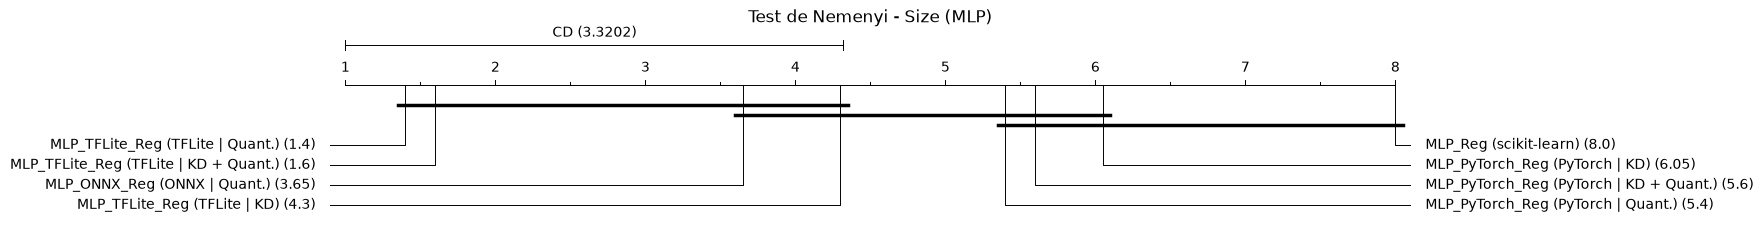
\includegraphics[width=1.0\textwidth]{mlp_reg_nemenyi_size.png}
    \caption{Diagrama de distancia crítica de Nemenyi para los MLP en regresión según el tamaño en disco.}
    \label{fig:mlp_reg_nemenyi_size}
\end{figure}
Mediante el análisis de distancias con el test de Nemenyi, se verifica la superioridad estrucural de TensorFlow Lite en
cuanto la optimización del almacenamiento físico, en particular con las variantes cuantizadas, como cabía esperar. Al
separarse significativamente de PyTorch en su conjunto, TFLite ofrece una reducción paramétrica imbatible frente a las
demás opciones.\\

\begin{figure}[htbp]
    \centering
    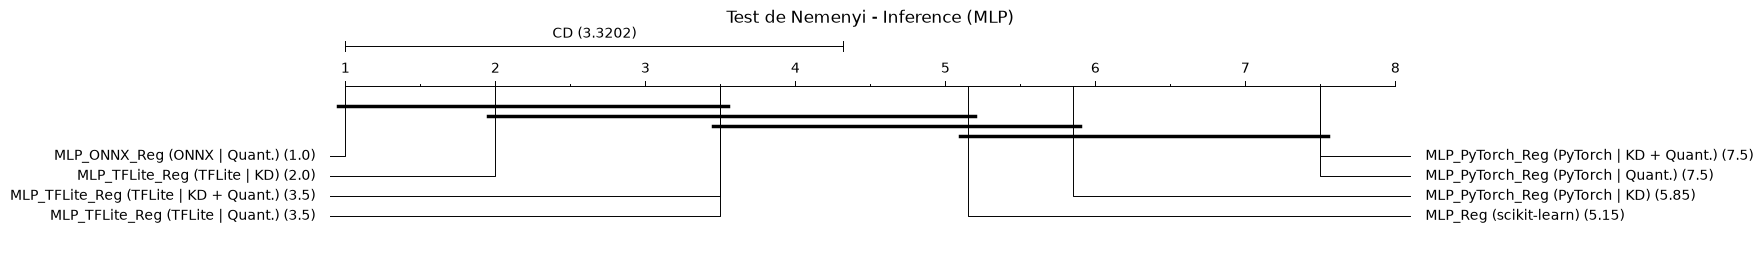
\includegraphics[width=1.0\textwidth]{mlp_reg_nemenyi_inference.png}
    \caption{Diagrama de distancia crítica de Nemenyi para los MLP en regresión según la el tiempo de inferencia.}
    \label{fig:mlp_reg_nemenyi_inference}
\end{figure}
Los resultados que presentan los tests de inferencia subrayan las concesiones ya estudiadas. Con ONNX Runtime y TFLite
liderando sin discusión la velocidad computacional, podemos confirmar el defecto que se lleva viendo a PyTprch arrastrar
durante todo el estudio. El sobrecoste de la decuantización dinámica de activaciones y el despacho de operaciones JIT
del motor de PyTorch penalizan su latencia de inferencia, situándolo en el último bloque estadístico.\\

La elección de una alternativa en regresión por parte del ingeniero, al igual que en clasificación, depende de los
factores analizados y de las restricciones de la plataforma de destino.
\begin{itemize}
  \item \textbf{Prioridad en la exactitud y fiabilidad del valor continuo}. En este caso, optar por PyTorch con
  destilación de conocimiento pura seguiría representando la alternativa preferible. Se trata del modelo que mejor
  protege la escala predictiva, evitando fluctuaciones anómalas en las salidas mientras mantiene el modelo bajo un
  límite de peso razonable.
  \item \textbf{Prioridad en el almacenamiento y la inferencia}. De nuevo, si existen restricciones especialmente
  serveras, la solución óptima es TensorFlow Lite en su versión híbrida, en los casos más excesivos. Pierde en
  rendimiento predictivo frente a PyTorch, pero mantiene un tamaño de archivo mínimo y una latencia ligeramente inferior.
\end{itemize}

\section{Compromisos y escalabilidad}
Tal y como se anticipaba al inicio de este capítulo, tras haber diseccionado el comportamiento individual de cada
framework y técnica de optimización a través del contraste estadístico de Friedman y Nemenyi, corresponde ahora
sintetizar todos estos hallazgos bajo un prisma multiobjetivo. Mientras que las secciones anteriores han evaluado cada
métrica de forma aislada, ningún sistema de despliegue real puede permitirse optimizar una sola de ellas ignorando el
resto. Por ejemplo, un modelo perfecto en F1-score pero inasumible en memoria es tan inviable para el
\textit{edge computing} como uno instantáneo pero inútil. El presente apartado aborda, por tanto, la búsqueda de la
frontera óptima de compromiso, así como el estudio de cómo la complejidad y el volumen de los datos condicionan la
escalabilidad de las soluciones evaluadas.
%A lo largo de las secciones previas, el rendimiento predictivo, la huella de memoria y la latencia computacional se han
%diseccionado de forma mayoritariamente aislada o mediante comparativas directas entre pares de frameworks. Sin embargo,
%el diseño de sistemas TinyML y de inteligencia artificial en el borde constituye, por definición, un problema de
%optimización multiobjetivo. En entornos de producción real, rara vez es posible maximizar una métrica sin degradar otra.\\

%Por consiguiente, esta sección finaliza el análisis empírico abordando la evaluación conjunta de estos factores,
%empleando para ello el cálculo del frente de Pareto. Asimismo, se evalúa la escalabilidad de los modelos analizando cómo
%la complejidad intrínseca de los conjuntos de datos impacta en la viabilidad operativa de las arquitecturas evaluadas.%

\subsection{Metodología del análisis multiobjetivo}
El análisis se apoya en dos herramientas complementarias, ambas implementadas de forma programática para garantizar la
reproducibilidad y la actualización automática ante cualquier variación en los datos de origen.\\

En primer lugar, se emplea el concepto del frente de Pareto. Dado un conjunto de modelos caracterizados por su tamaño
en disco (KB) y su rendimiento predictivo (F1 o $R^2$, según la tarea), un modelo pertenece a la frontera óptima si
ningún otro modelo evaluado lo supera simultáneamente en ambas dimensiones, de modo que este límite está formado por
aquellos modelos que no son ``dominados''. Formalmente, ordenando el conjunto de candidatos de forma ascendente por
tamaño, un modelo se incorpora a la frontera si su rendimiento predictivo supera estrictamente al del mejor candidato
visto hasta ese punto del recorrido. El resultado es una secuencia de modelos que representa, para cada nivel de tamaño,
la mejor opción disponible: cualquier otro modelo del estudio es, o bien más grande sin ser mejor, o bien peor sin ser
más pequeño. La latencia de inferencia, tercera variable del compromiso, se codifica en estos gráficos mediante el
tamaño de la burbuja de cada punto, permitiendo una lectura simultánea de las tres dimensiones sin necesidad de
recurrir a una representación tridimensional.\\

Es importante señalar una diferencia metodológica deliberada frente al bloque de contraste estadístico previo. Si bien
para los tests de Friedman y Nemenyi era recomendable aislar comparaciones limpias entre subconjuntos homogéneos para no
confundir el efecto del framework con el del algoritmo o la técnica de compresión, el cálculo del frente de Pareto
persigue el objetivo contrario: identificar la mejor opción de despliegue en términos absolutos, para lo cual es
imprescindible enfrentar todos los candidatos disponibles a la vez. Trocear este análisis en los mismos subconjuntos que
los tests estadísticos generaría fronteras locales que no permitirían responder a la pregunta relevante en esta fase:
``de entre todo lo evaluado, ¿qué elijo?''.\\

En segundo lugar, se estudia la escalabilidad del ecosistema, entendida como la sensibilidad de las métricas de
eficiencia, tamaño y latencia, frente a dos ejes de complejidad de los datos: la dimensionalidad, medida como el número
de características de entrada, y el volumen, medido como el número de instancias del conjunto de datos. Para cada eje
se han generado representaciones gráficas, tanto estáticas como interactivas, que relacionan dicha variable de
complejidad con el tamaño y la latencia de todos los modelos evaluados, coloreados por framework.

\subsection{Frente de Pareto}
\subsubsection{Clasificación}
\begin{figure}[htbp]
    \centering
    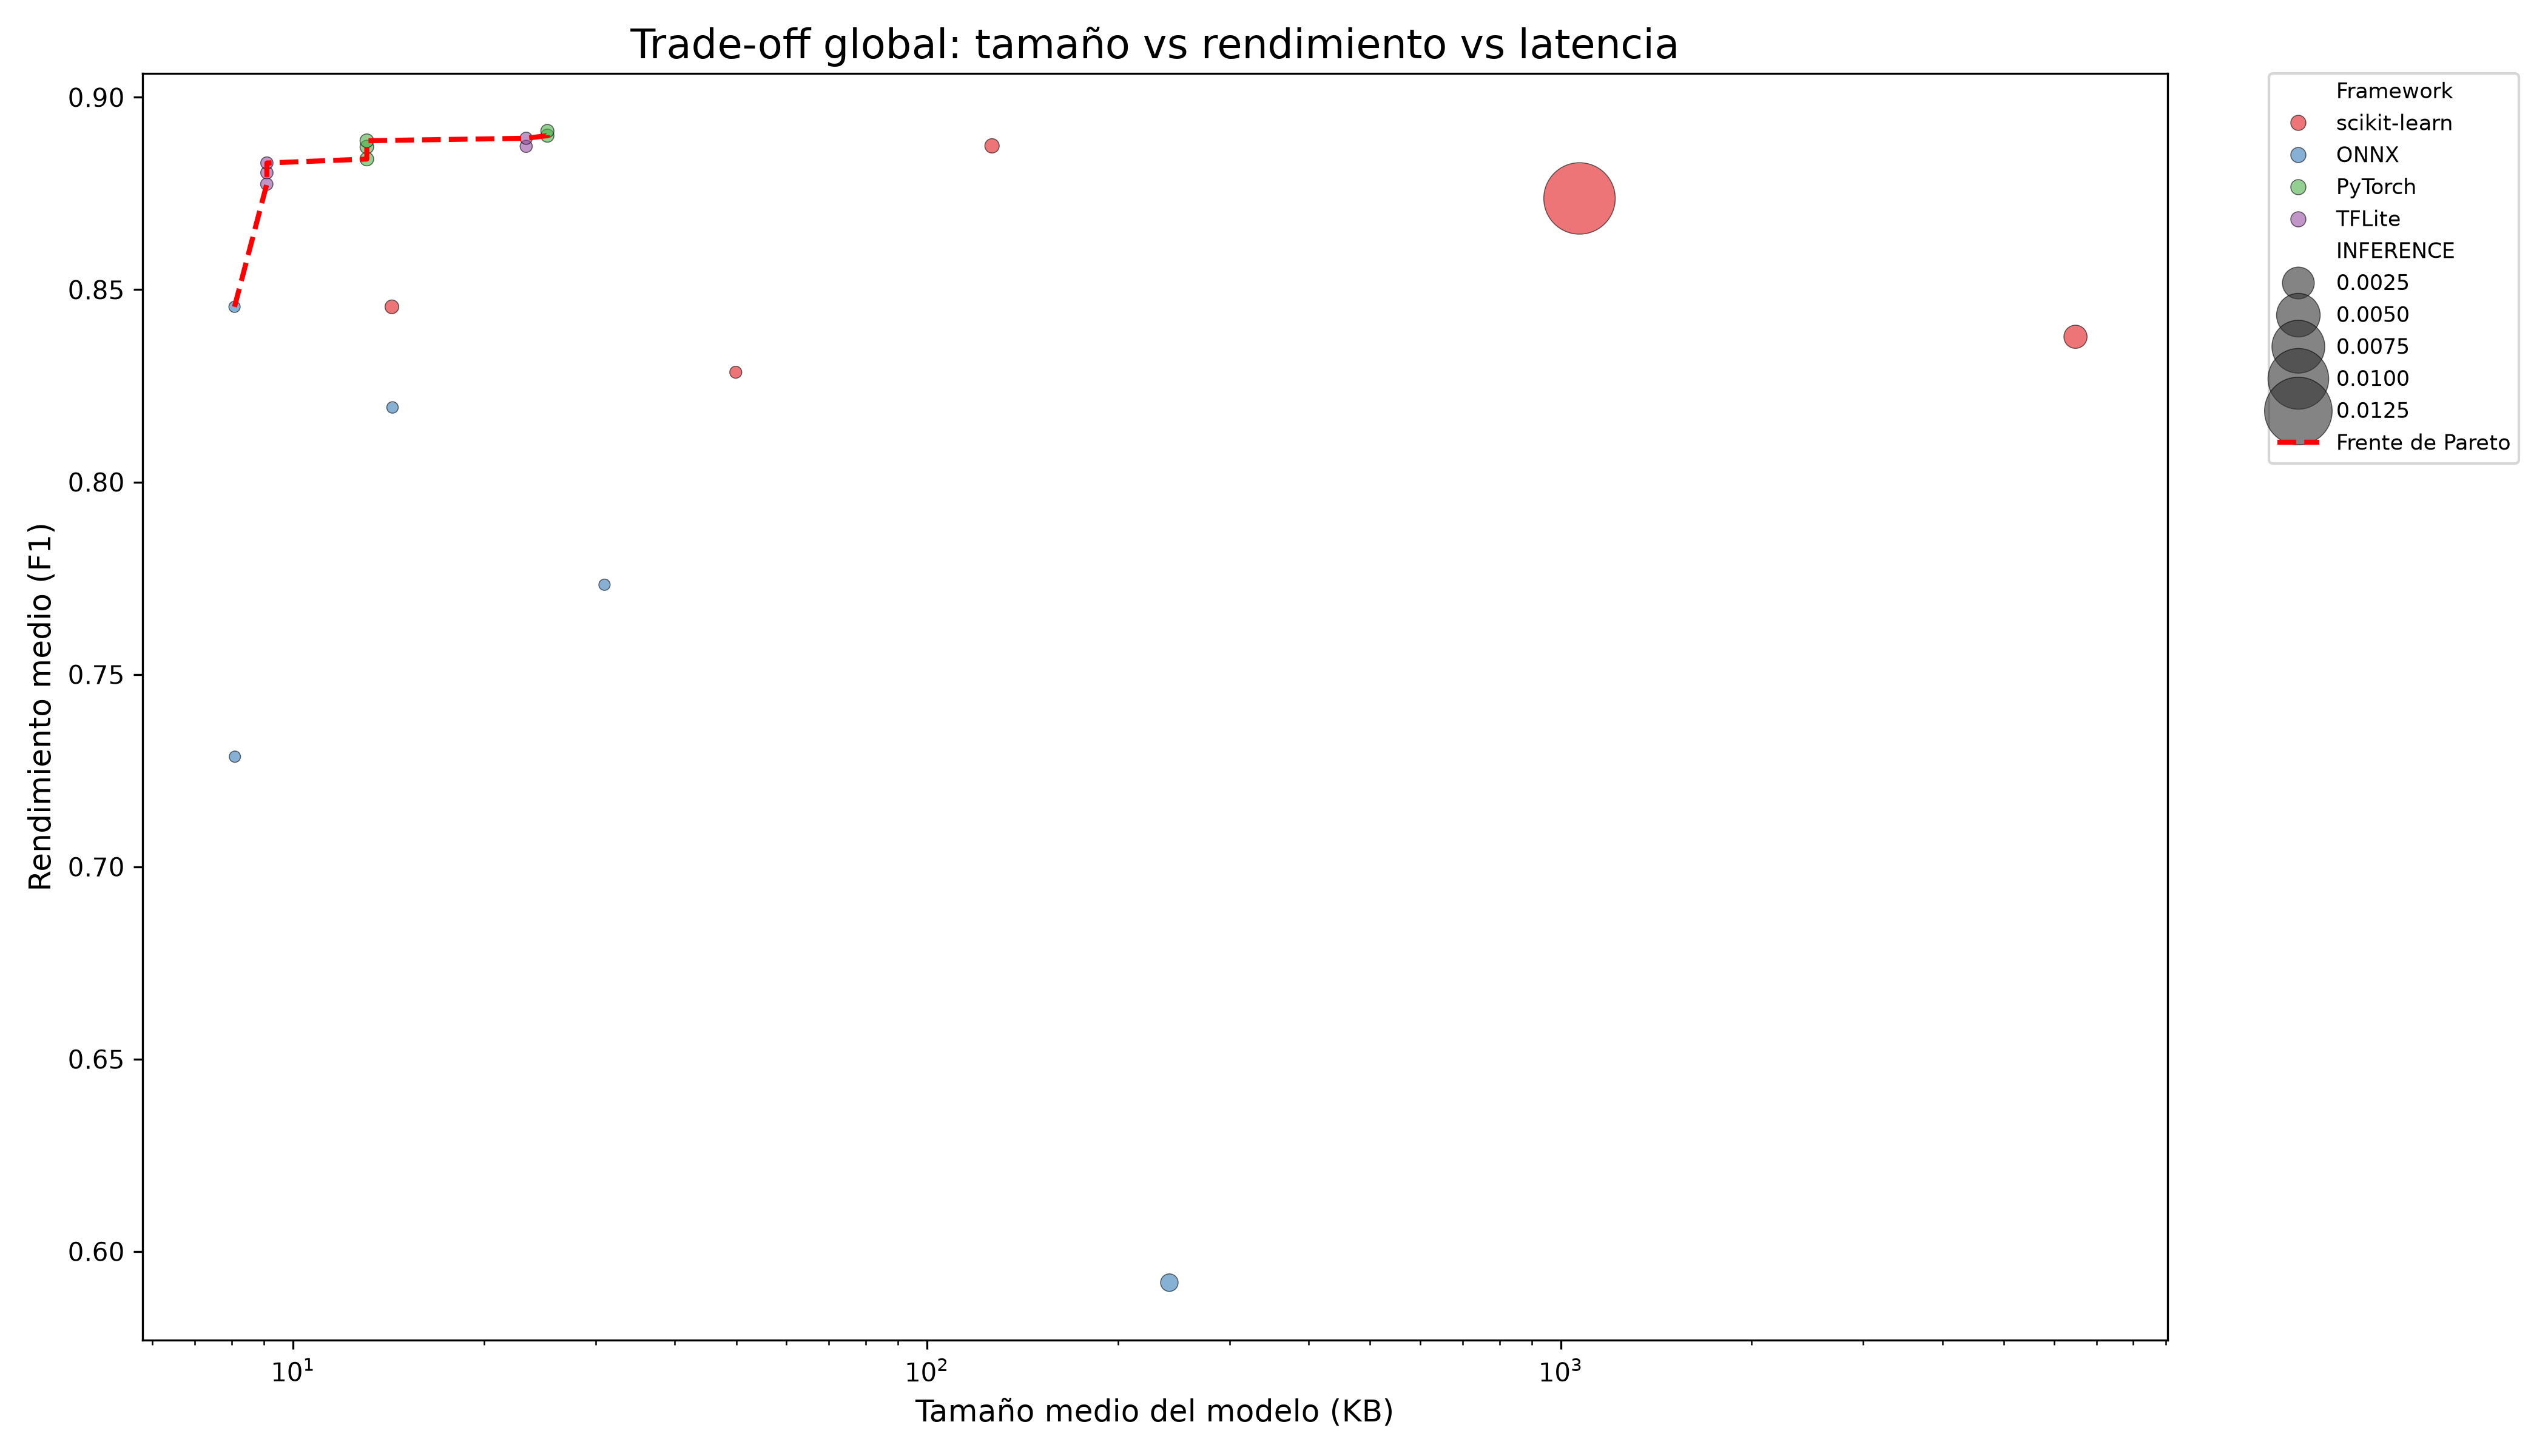
\includegraphics[width=1.0\textwidth]{global_tradeoff_pareto_class.png}
    \caption{Frente de Pareto para clasificación.}
    \label{fig:pareto_class}
\end{figure}
Con un primer vistazo al gráfico de compromisos en clasificación, se observa que el frente de Pareto se localiza en la
lo que sugiere que los modelos que lo conforman son especialmente óptimos en este caso. Al haber una notable dispersión
de arquitecturas en el espacio, esta vista no permite apreciar con claridad qué modelos concretos conforman la frontera.
Para solventar esta limitación, se ha generado un segundo gráfico que amplía la zona de interés, permitiendo identificar
los modelos seleccionados. Al mismo tiempo, mediante el gráfico interactivo generado con Plotly, es posible inspeccionar
los modelos uno a uno para ver sus detalles al completo.

\newpage
\begin{figure}[htbp]
    \centering
    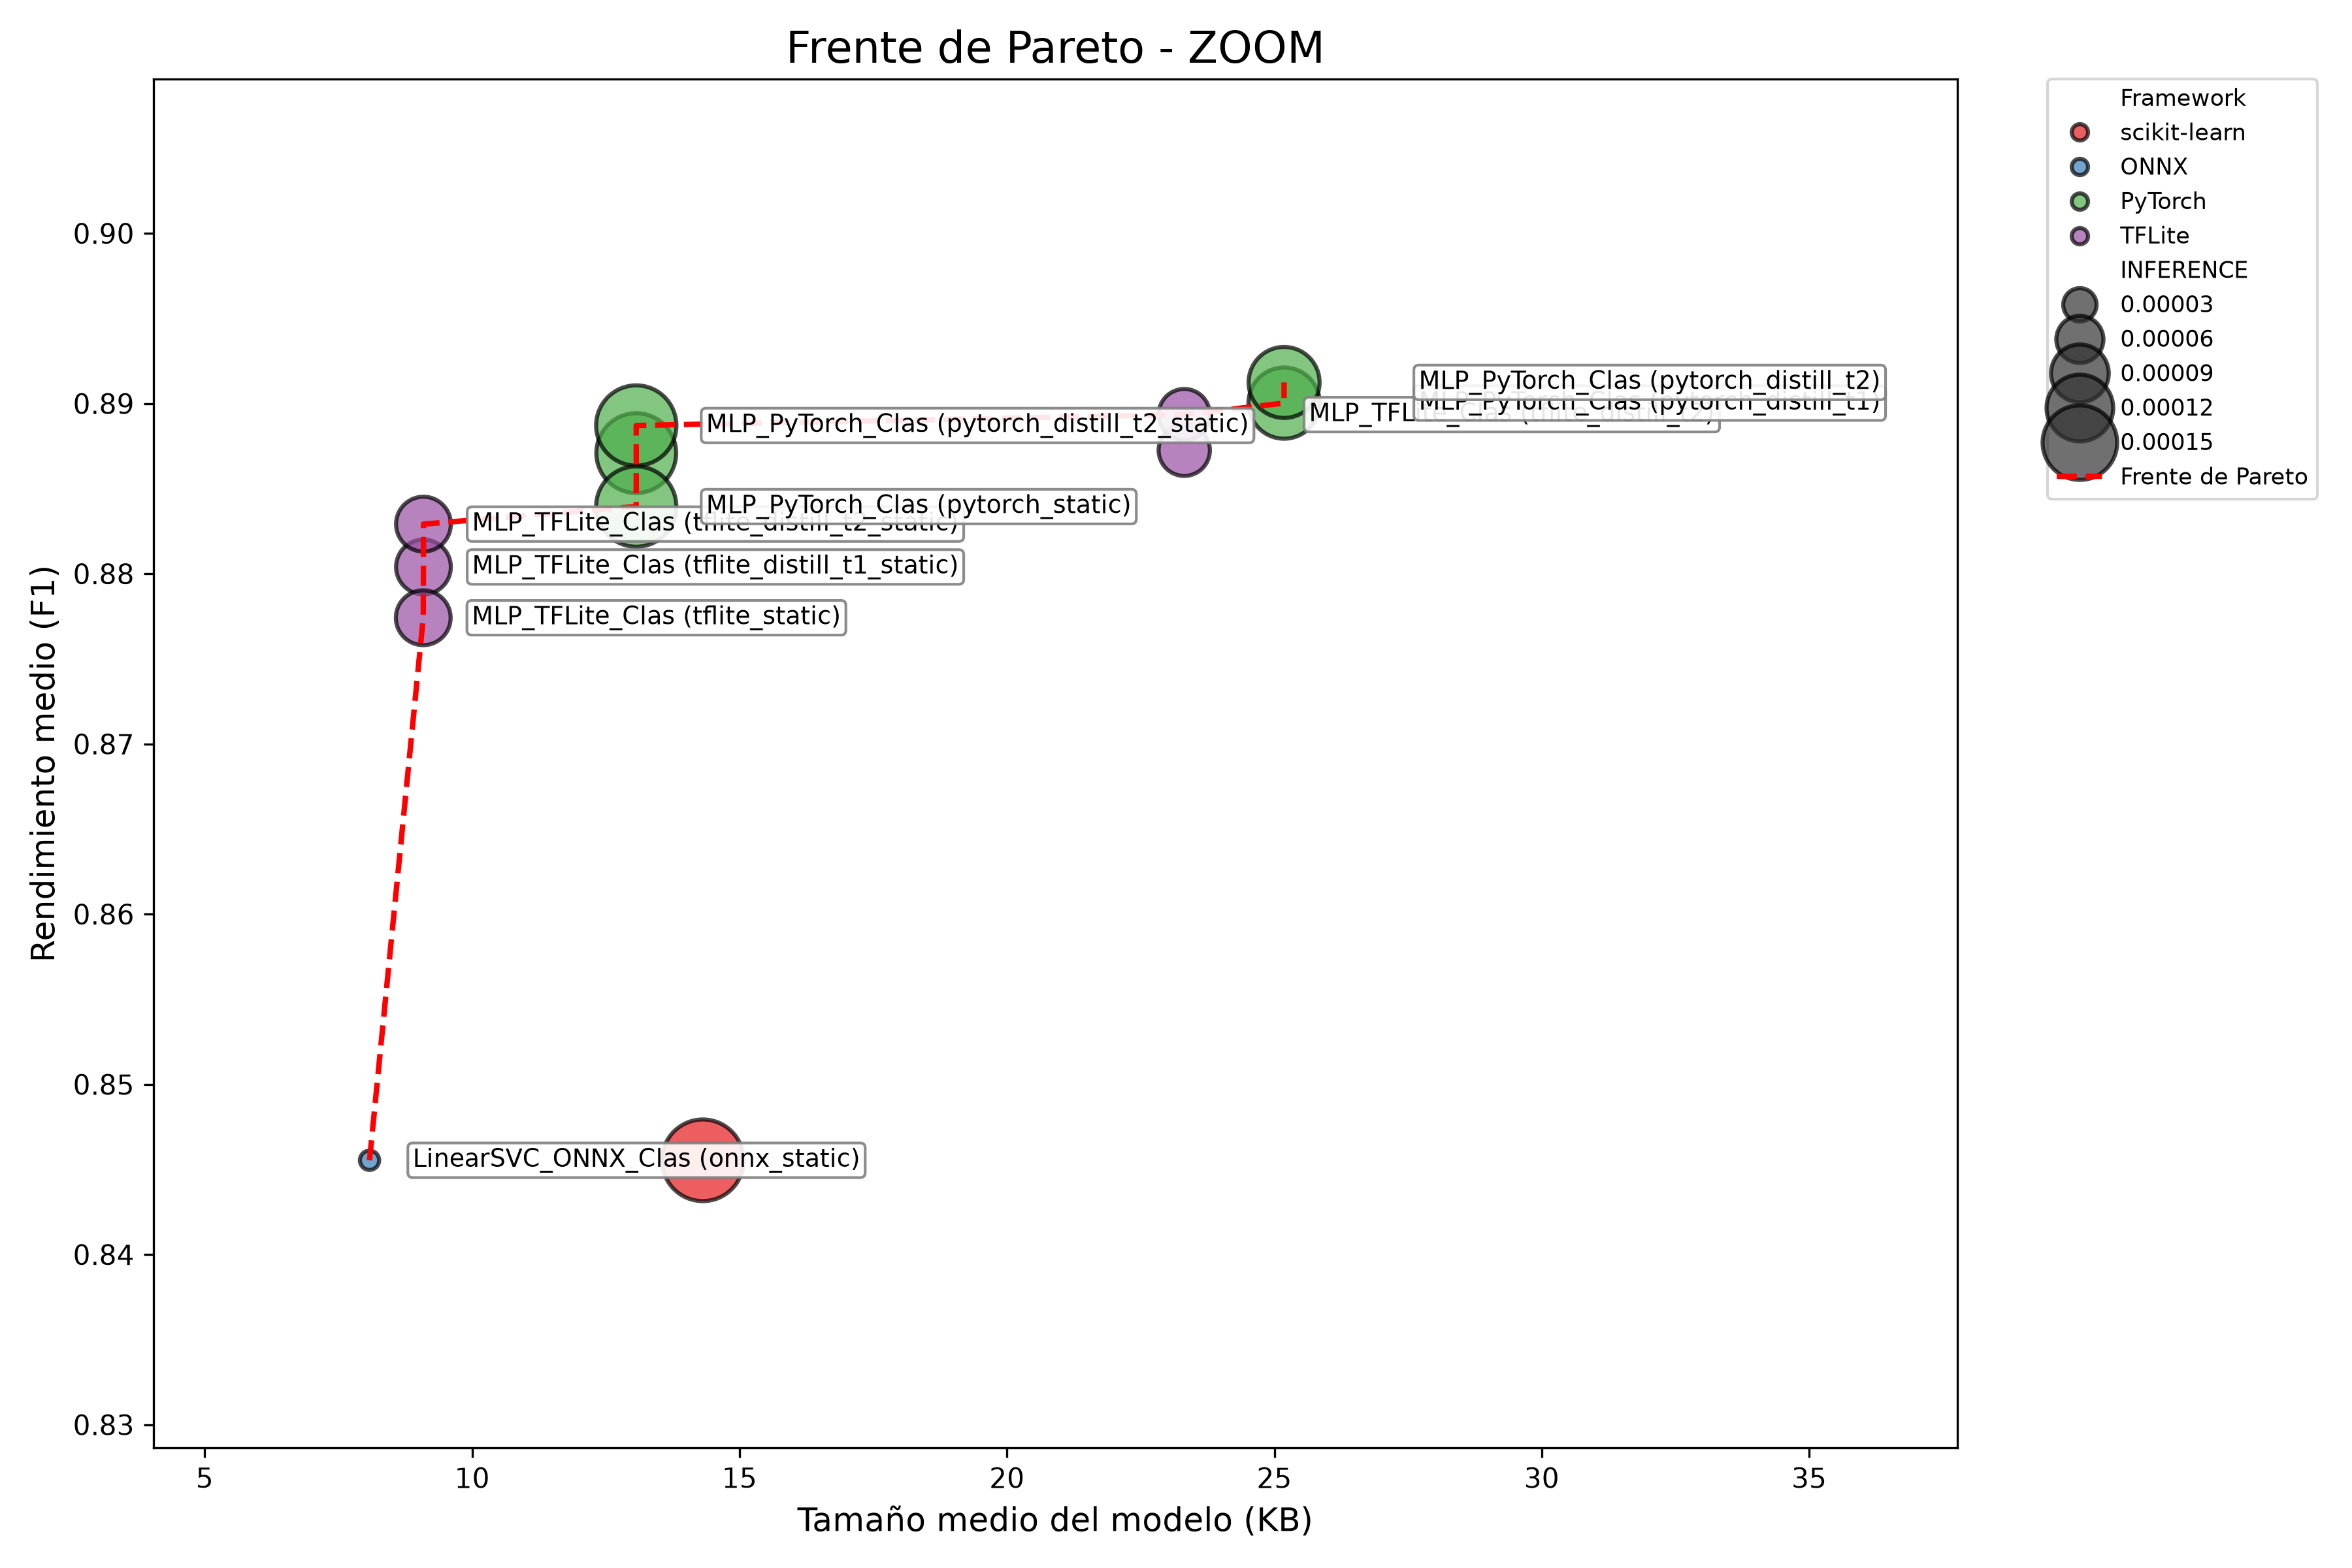
\includegraphics[width=1.0\textwidth]{global_tradeoff_pareto_ZOOM_class.png}
    \caption{Frente de Pareto ampliado para clasificación.}
    \label{fig:pareto_zoom_class}
\end{figure}

Haciendo uso del diagrama interactivo, se distinguen los siguientes modelos en el frente de Pareto, ordenador de menor a
mayor F1 y tamaño en disco.
\begin{table}[htbp]
  \centering
  \begin{tabularx}{\textwidth}{Xccc}
    \hline
    \textbf{Modelo} & \textbf{F1} & \textbf{Inferencia (ms)} & \textbf{Tamaño (KB)} \\
    \hline
    LinearSVC (ONNX) & 0.84554 & 0.01  & 8.08135  \\
    TF quant.               & 0.87741 & 0.081 & 9.08594  \\
    TF quant. $+$ T1        & 0.88040 & 0.081 & 9.08984  \\
    TF quant. $+$ T2        & 0.88292 & 0.081 & 9.08984  \\
    PT quant.               & 0.88395 & 0.174 & 13.06836 \\
    PT quant. $+$ T1        & 0.88709 & 0.172 & 13.06875 \\
    PT quant. $+$ T2        & 0.88871 & 0.174 & 13.06875 \\
    TF T2                   & 0.88935 & 0.071 & 23.31563 \\
    PT T1                   & 0.89003 & 0.137 & 25.18242 \\
    PT T2                   & 0.89124 & 0.136 & 25.18242 \\
    \hline
  \end{tabularx}
  \caption{Modelos del frente de Pareto en clasificación.}
  \label{tab:pareto_global_clas}
\end{table}

La lectura de la frontera permite extraer conclusiones de interés. De los cinco algoritmos clásicos evaluados, es solo
LinearSVC en su versión exportada a ONNX el que logra sobrevivir al filtro de Pareto, ocupando el extremo de menor
tamaño a cambio del F1 más modesto del frente. Ninguno de los demás modelos tradicionales consiguen entrar en este grupo,
ya que cada uno de ellos es, o bien más pesado sin mejorar alguna configuración de MLP nativa, o bien más ligero pero
peor que LinearSVC.\\

A partir de aquí, la totalidad del recorrido óptimo está conformado por variantes del MLP en PyTorch y TensorFlow Lite,
alternándose en función del punto de la curva. TensorFlow domina el tramo más económico al mostar menores tamaños y
latencias, mientras que PyTorch se impone en el tramo superior de rendimiento, con F1-scores más altos a cambio de un
ligero incremento en el tamaño y la latencia.\\

Cabe destacar que, salvo por la configuración de TensorFlow con cuantización pura con $T=1$, los modelos MLP de PyTorch
y TensorFlow en su totalidad entran en el frente de Pareto, lo que evidencia que la destilación de conocimiento y la
cuantización son técnicas eficaces para mejorar la eficiencia de los modelos sin degradar su capacidad predictiva, a la
vez que necesarias para hacer al MLP competitivo en el espacio de despliegue. Analizando los resultados que ofrecen
estos, modelos, podemos hacer algunos descartes sin ningún reparo. En cuanto a las configuraciones con cuantización de
TensorFlow, las tres presentan inferencias y tamaños idénticos, por lo que, fijándonos únicamente en el F1-score, la
alternativa que combina cuantización y destilación de conocimiento con $T=2$ es la que obtiene la mejor puntuación, de
modo que pueden desecharse las otras dos. El caso de PyTorch es idéntico, tanto en sus configuraciones puras como en las
híbridas. Añadir la destilación de conocimiento a la ejecución siempre es mejor que no hacerlo y aplicar solo la
cuantización. Asimismo, a la hora de aplicar la destilación, una temperatura de 2 permitirá obtener los mejores
resultados.

\subsubsection{Regresión}
\begin{figure}[htbp]
    \centering
    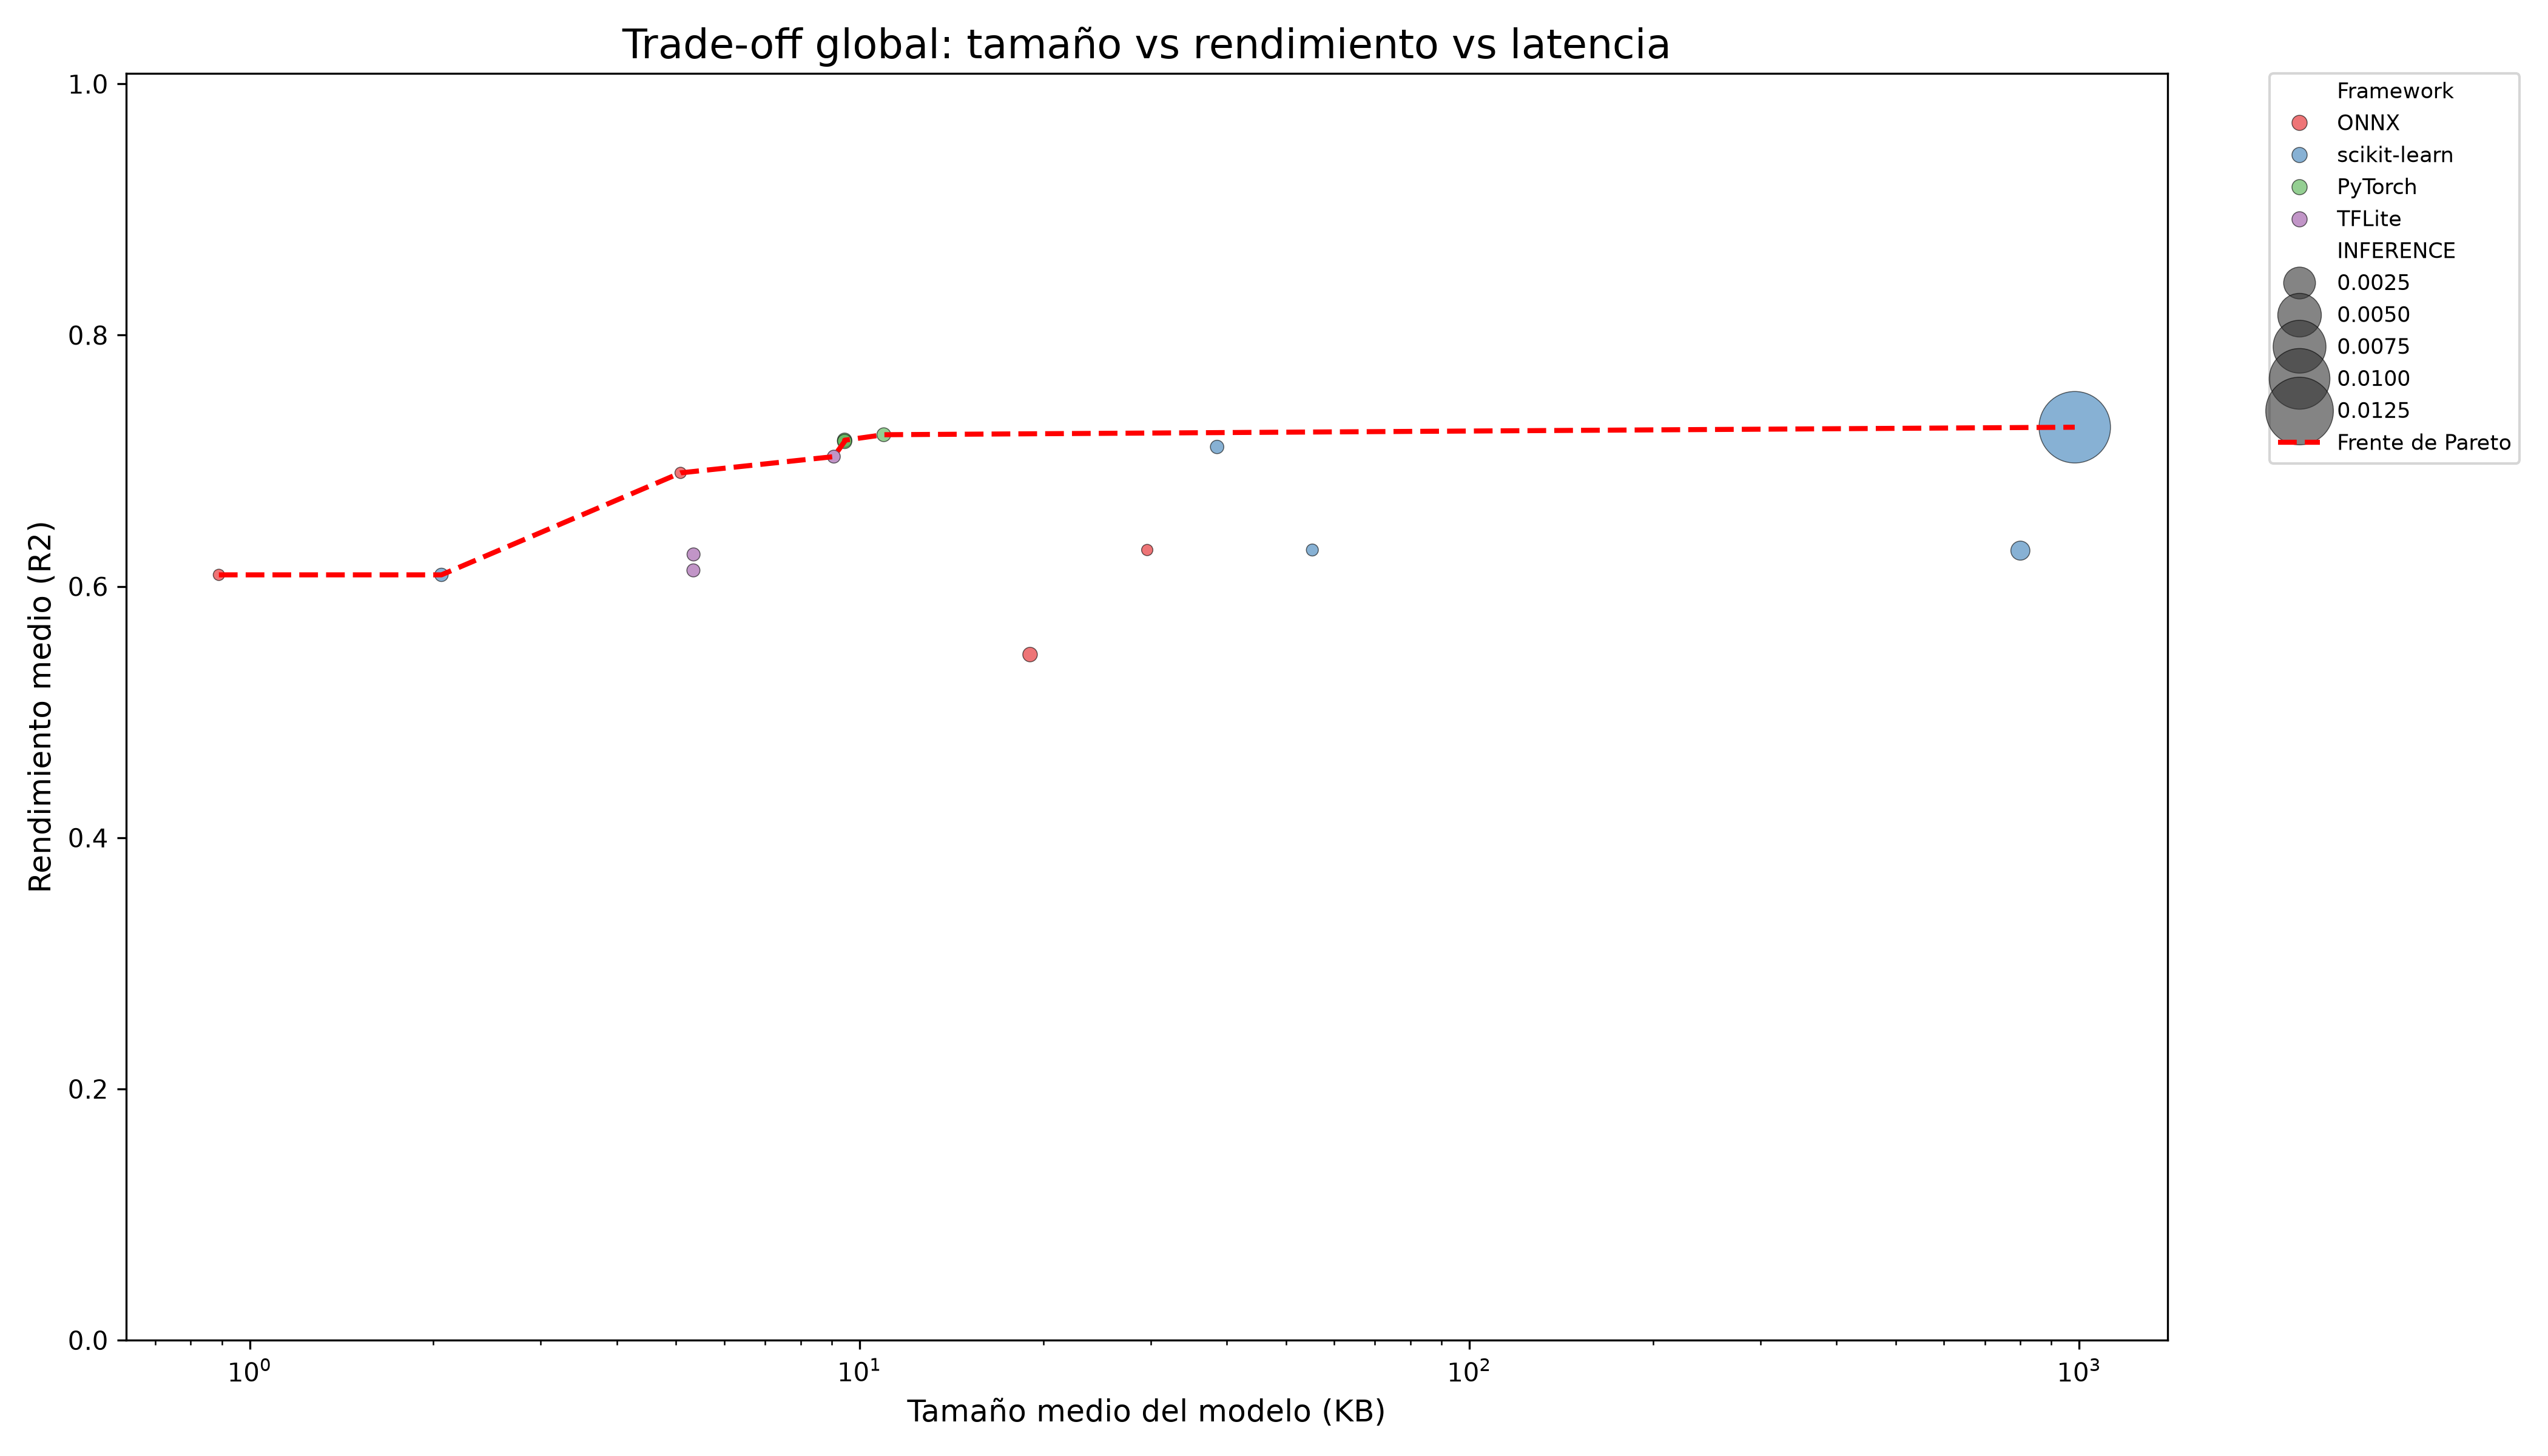
\includegraphics[width=1.0\textwidth]{global_tradeoff_pareto_reg.png}
    \caption{Frente de Pareto para regresión.}
    \label{fig:pareto_reg}
\end{figure}
Igual que antes, generamos una vista ampliada de la zona de interés para poder identificar los modelos que conforman el
frente de Pareto.

\newpage
\begin{figure}[htbp]
    \centering
    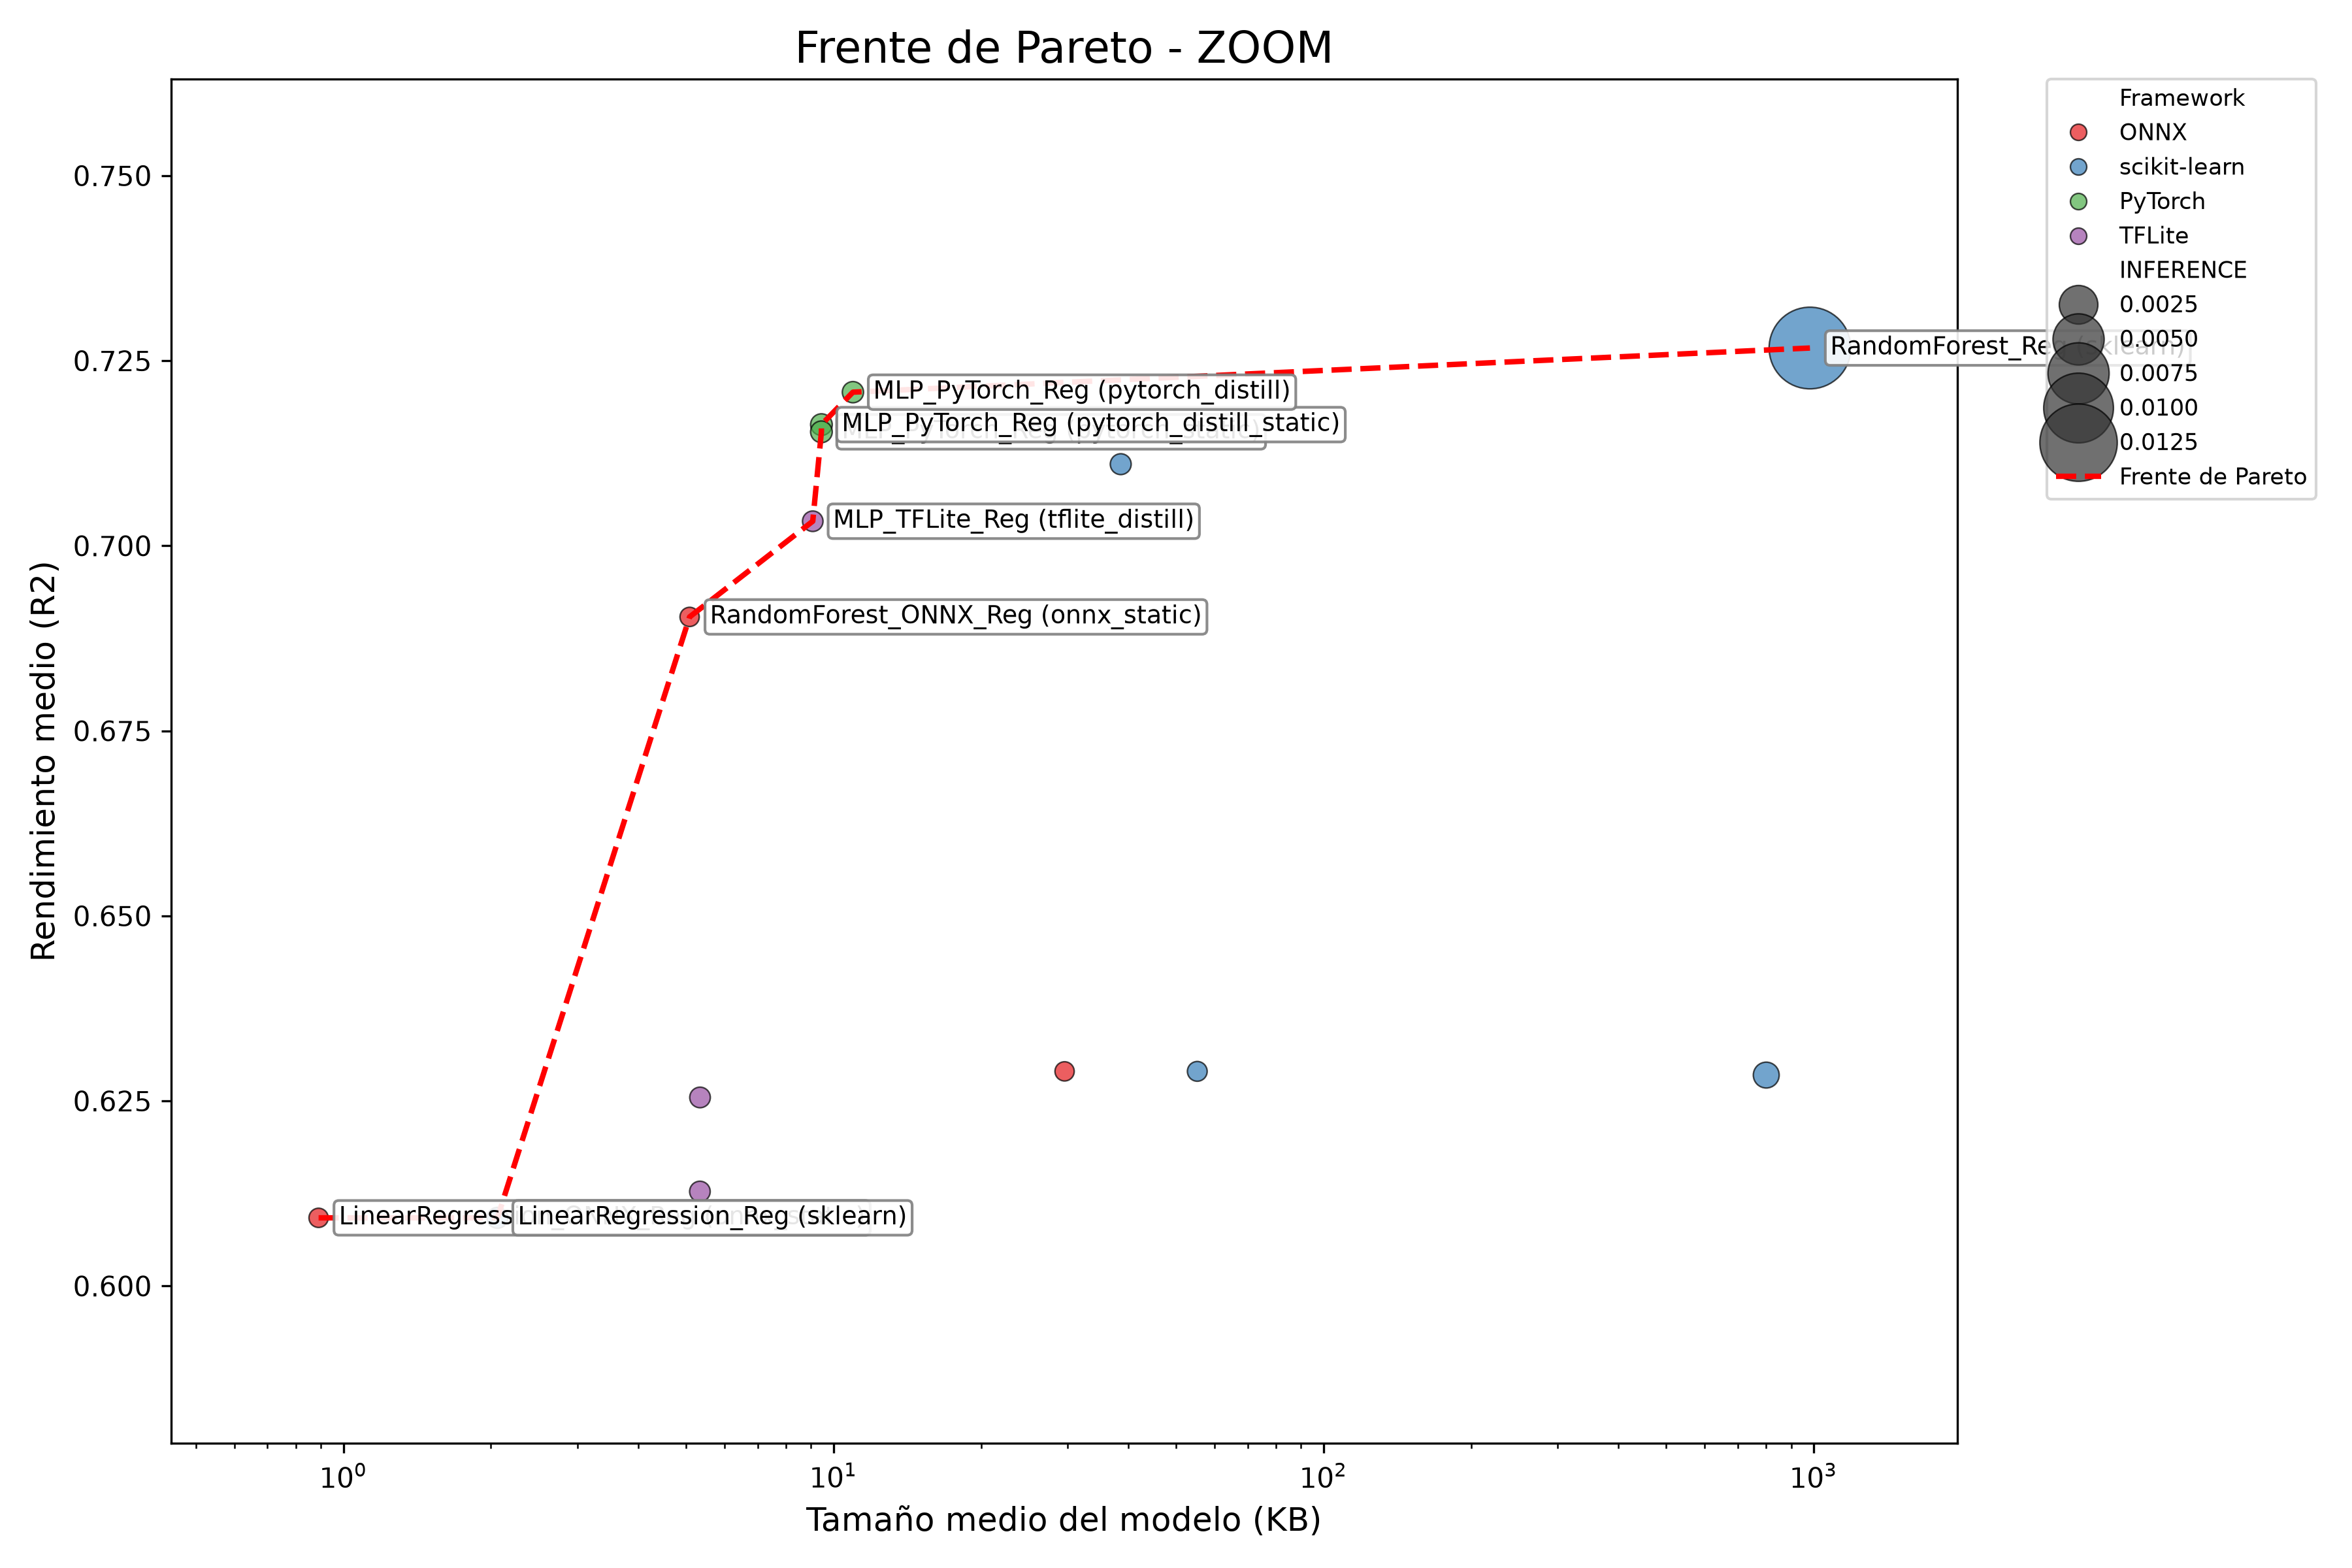
\includegraphics[width=1.0\textwidth]{global_tradeoff_pareto_ZOOM_reg.png}
    \caption{Frente de Pareto ampliado para regresión.}
    \label{fig:pareto_zoom_reg}
\end{figure}
La frontera de regresión es sensiblemente más corta que la de clasificación, notando que en el tramo final se decide
incluir al Random Forest base de scikit-learn, viéndose el tamaño previo multiplicado por casi 90 veces para obtener una
mejora de apenas 0.006 en R$^2$, una ganancia marginal que no debería suponer una significancia estadística, hablando en
términos de los tests previos. Por tanto, este Random Forest debería ser candidato a eliminarse del frente de Pareto
pese a obtener un R$^2$ ligeramente superior al de los modelos MLP, puesto que su peso y dependencia del intérprete de
Python no hacen posible su despliegue en un microcontrolador.\\

\begin{table}[htbp]
  \centering
  \begin{tabularx}{\textwidth}{Xccc}
    \hline
    \textbf{Modelo} & \textbf{R$^2$} & \textbf{Inferencia (ms)} & \textbf{Tamaño (KB)} \\
    \hline
    LinearReg (ONNX)            & 0.60921 & 0.01   & 0.88994   \\
    LinearReg (scikit-learn)    & 0.60921 & 0.153  & 2.06221   \\
    RandomForest (ONNX)         & 0.69039 & 0.01   & 5.08691   \\
    TF KD                       & 0.70331 & 0.12   & 9.07266   \\
    PT quant.                   & 0.71539 & 0.229  & 9.44961   \\
    PT quant. + KD              & 0.71637 & 0.228  & 9.45000   \\
    PT KD                       & 0.72075 & 0.188  & 10.95742  \\
    RandomForest (scikit-learn) & 0.72671 & 14.014 & 983.09521 \\
    \hline
  \end{tabularx}
  \caption{Modelos del frente de Pareto en regresión.}
  \label{tab:pareto_global_reg}
\end{table}

El resto del trayecto reproduce fielmente lo contemplado en clasificación. La exportación a ONNX domina el extremo más
ligero, PyTorch ocupa la zona de mejor rendimiento predictivo y TensorFlow Lite se sitúa en una posición intermedia. Por
otra parte, la destilación de conocimiento y la cuantización también replican su comportamiento. La pérdida de precisión
provocada por la cuantización es mitigada por la destilación, siendo la combinación de ambas preferible frente a la
cuantización aislada en cualquier caso.

\subsection{Escalabilidad respecto a la dimensionalidad y el volumen de datos}
El segundo eje analítico de esta sección evalúa la fortaleza de los algoritmos ante el aumento de la complejidad 
estructural de los datos de entrada. A través de diagramas de dispersión, se ha modelado cómo el número de instancias y 
el número de características de los datasets perturban la latencia y la memoria.   

\subsubsection{Impacto del número de características en latencia - Clasificación}
\begin{figure}[htbp]
    \centering
    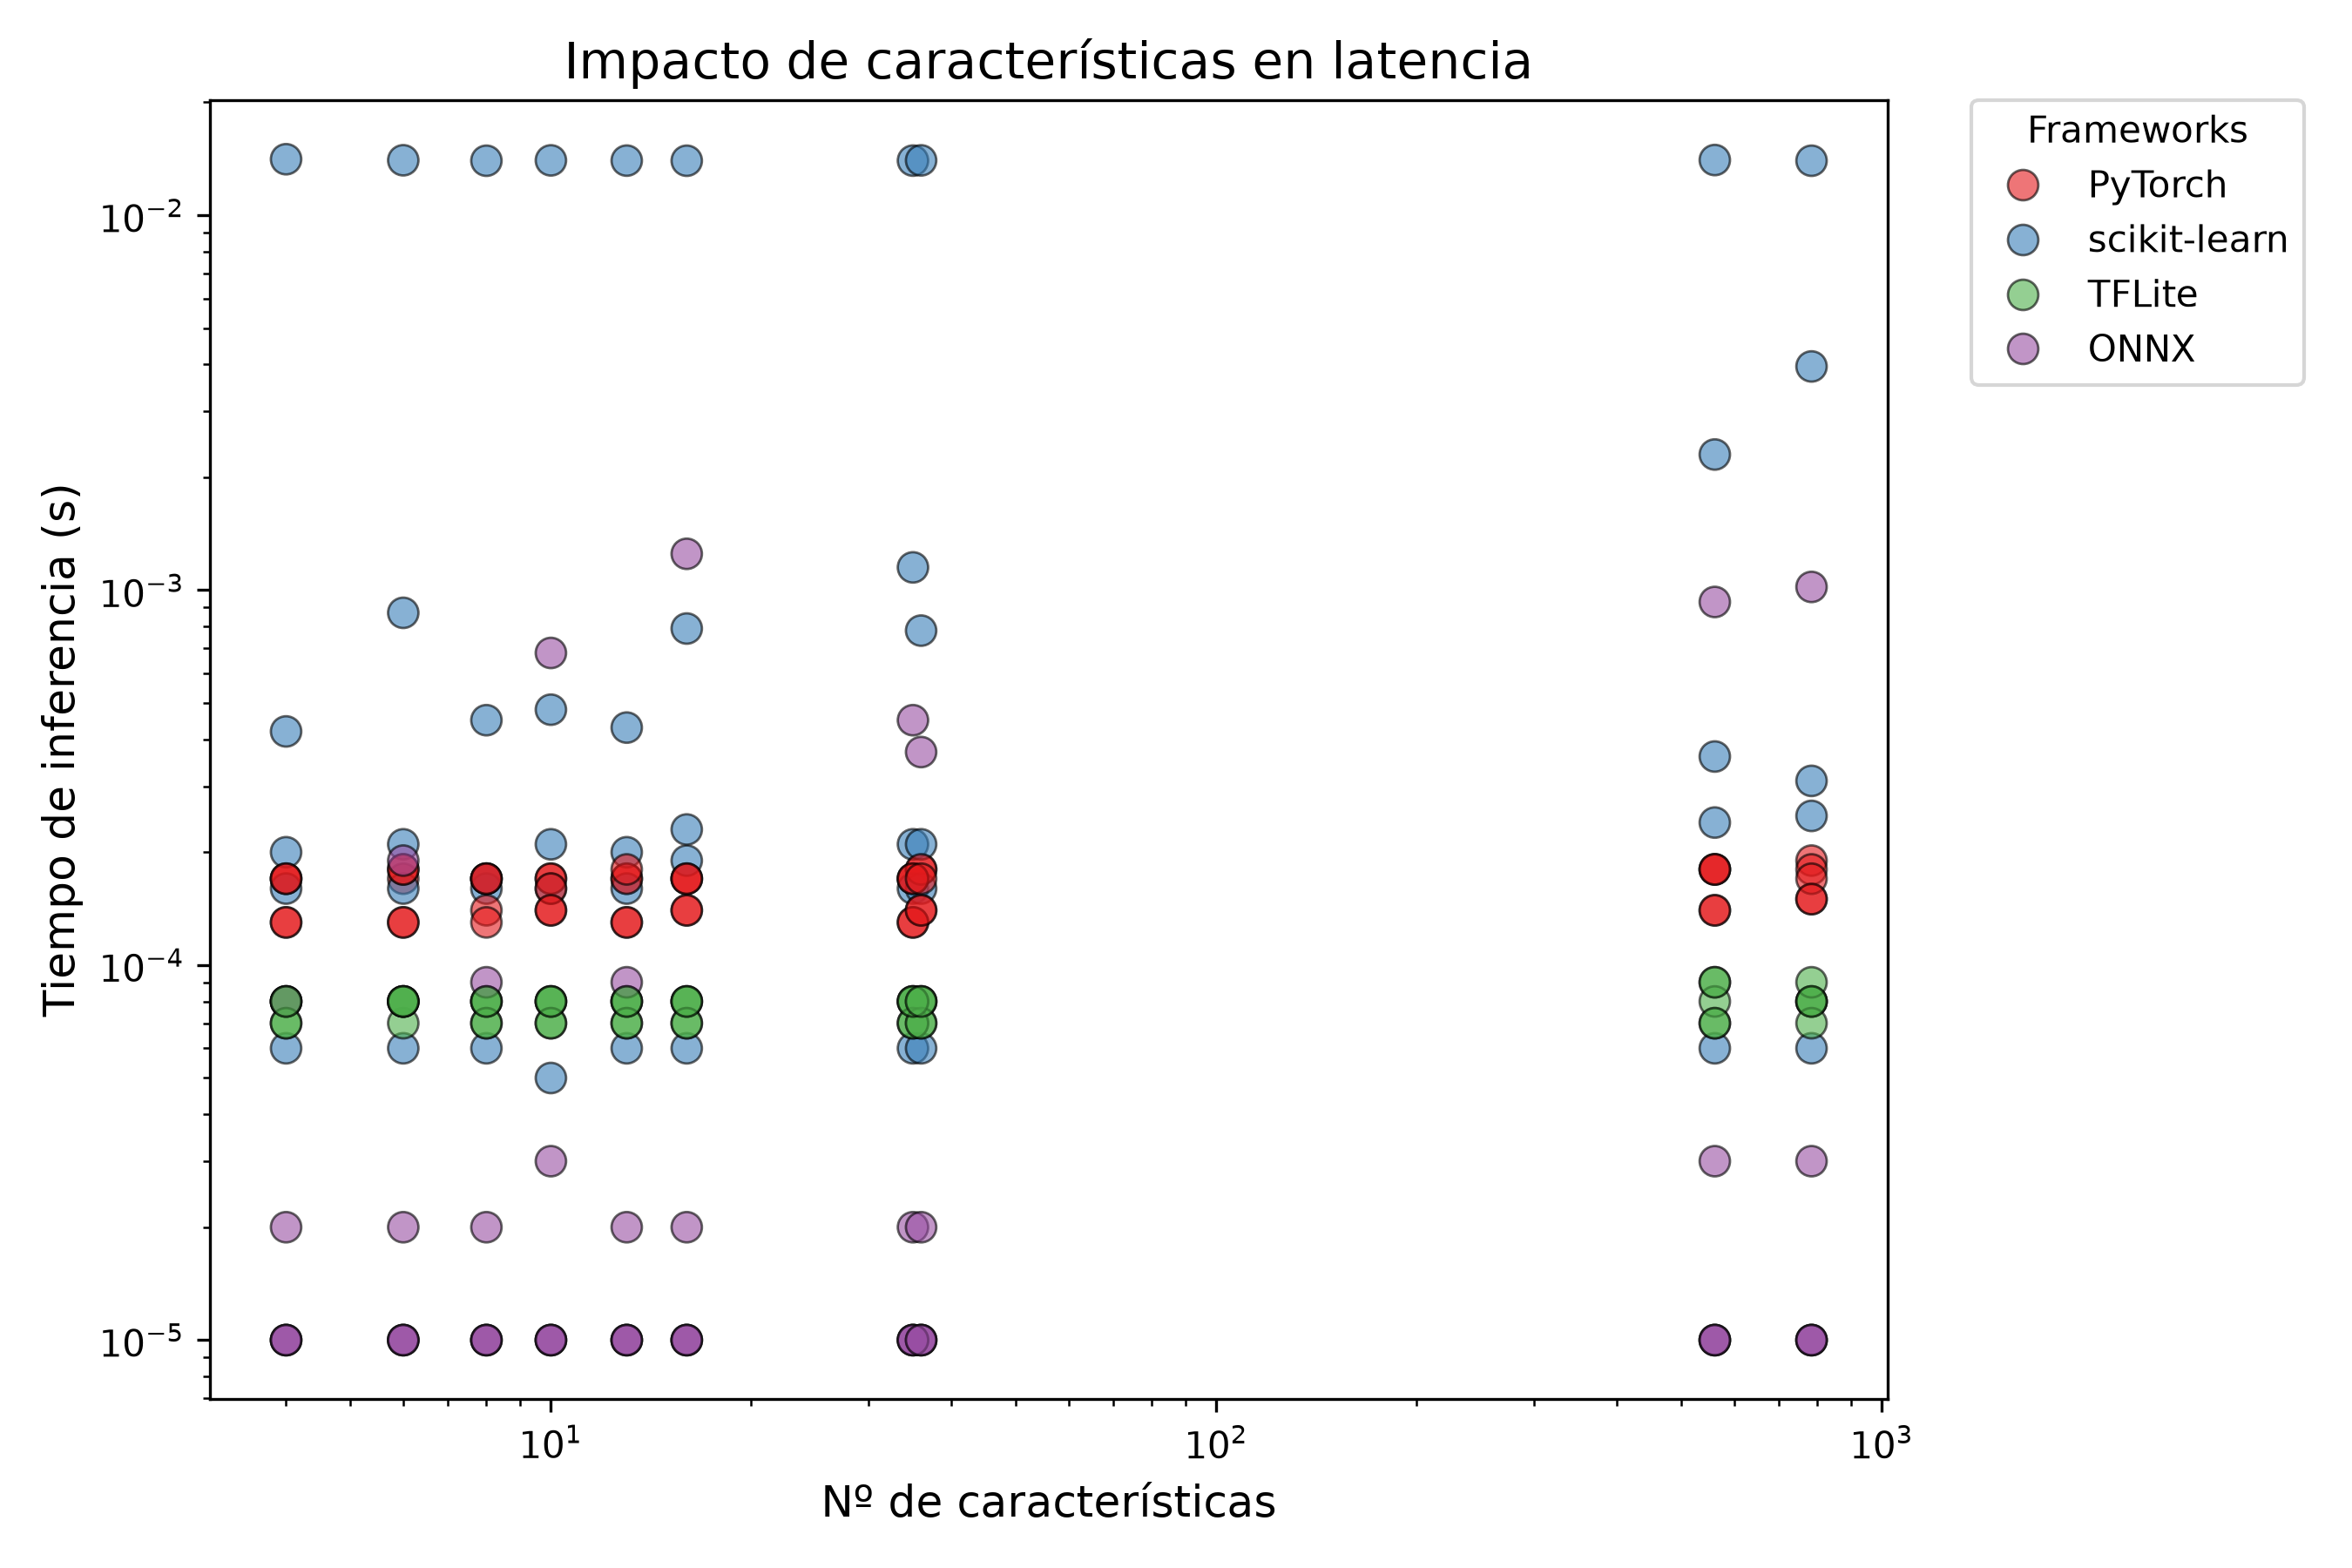
\includegraphics[width=1.0\textwidth]{complexity_features_latency_class.png}
    \caption{Relación entre el número de características y el tiempo de inferencia por framework en clasificación.}
    \label{fig:features_latency_class}
\end{figure}

\newpage
\subsubsection{Impacto del número de características en latencia - Regresión}
\begin{figure}[htbp]
    \centering
    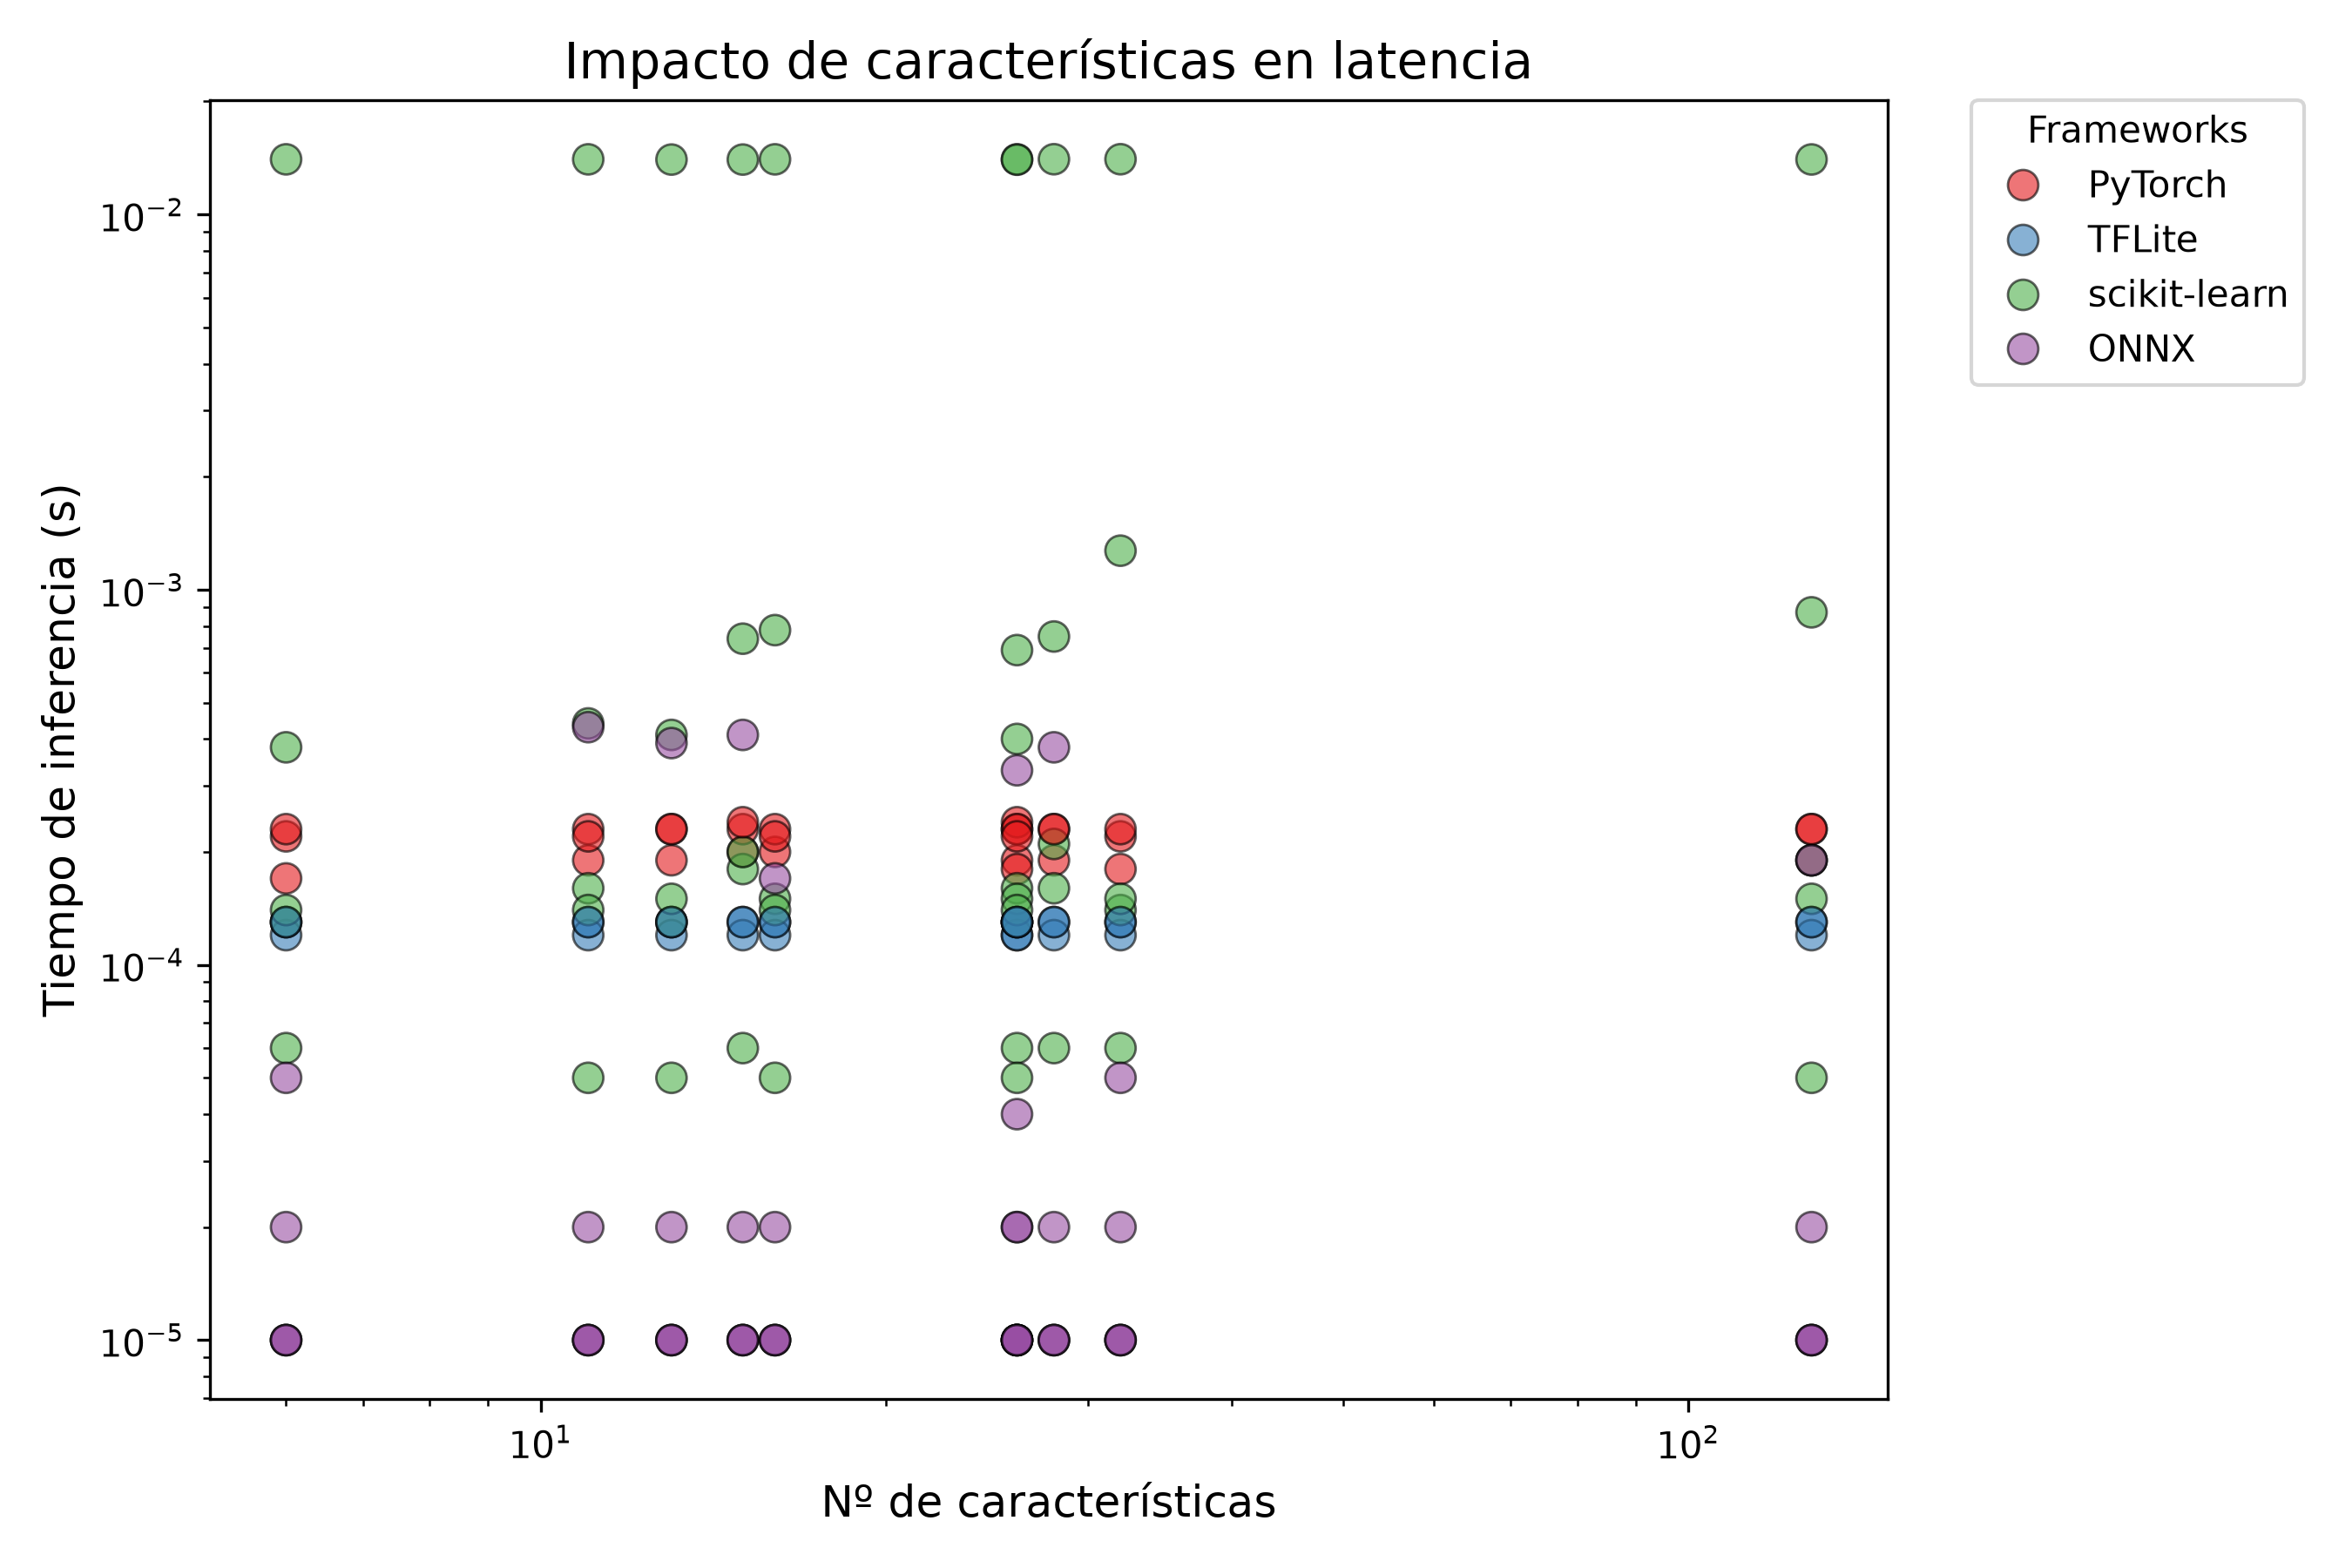
\includegraphics[width=1.0\textwidth]{complexity_features_latency_reg.png}
    \caption{Relación entre el número de características y el tiempo de inferencia por framework en regresión.}
    \label{fig:features_latency_reg}
\end{figure}

La primera pareja de gráficas, que enfrenta el número de características con la latencia de inferencia, muestra que,
para la inmensa mayoría de los algoritmos evaluados, la latencia no crece de forma visible con el número de
características, ni en clasificación ni en regresión. En su lugar, cada framework ocupa una banda prácticamente
horizontal y constante a lo largo de todo el eje, con independencia de si el modelo procesa 4 o 784 características.
Esto se explica porque, para una única inferencia sobre modelos de dimensiones tan reducidas como los aquí evaluados, el
coste puramente aritmético de la multiplicación matricial resulta órdenes de magnitud inferior a la sobrecarga fija del
propio motor de ejecución, que es la que realmente domina el tiempo medido. Dentro del rango de dimensionalidad
estudiado, qué framework y algoritmo se emplea pesa mucho más sobre la latencia que cuántas características tenga el
problema.\\

Se observa una excepción más clara, correspondiente a k-NN, más acentuado en el caso de la clasificación, con puntos
que despegan hacia arriba en los datasets con más características, HAR y MNIST, alcanzando latencias varias veces
superiores a las del resto de algoritmos clásicos. Al tratarse de un método de aprendizaje perezoso, cada predicción
exige calcular explícitamente la distancia euclídea componente a componente frente a las instancias almacenadas, por
lo que su coste sí escala de forma más visible con el número de características, a diferencia de los métodos
paramétricos, cuyo coste aritmético queda enmascarado por la sobrecarga fija del entorno de ejecución.

\subsubsection{Impacto del número de características en el tamaño del modelo - Clasificación}
\begin{figure}[htbp]
    \centering
    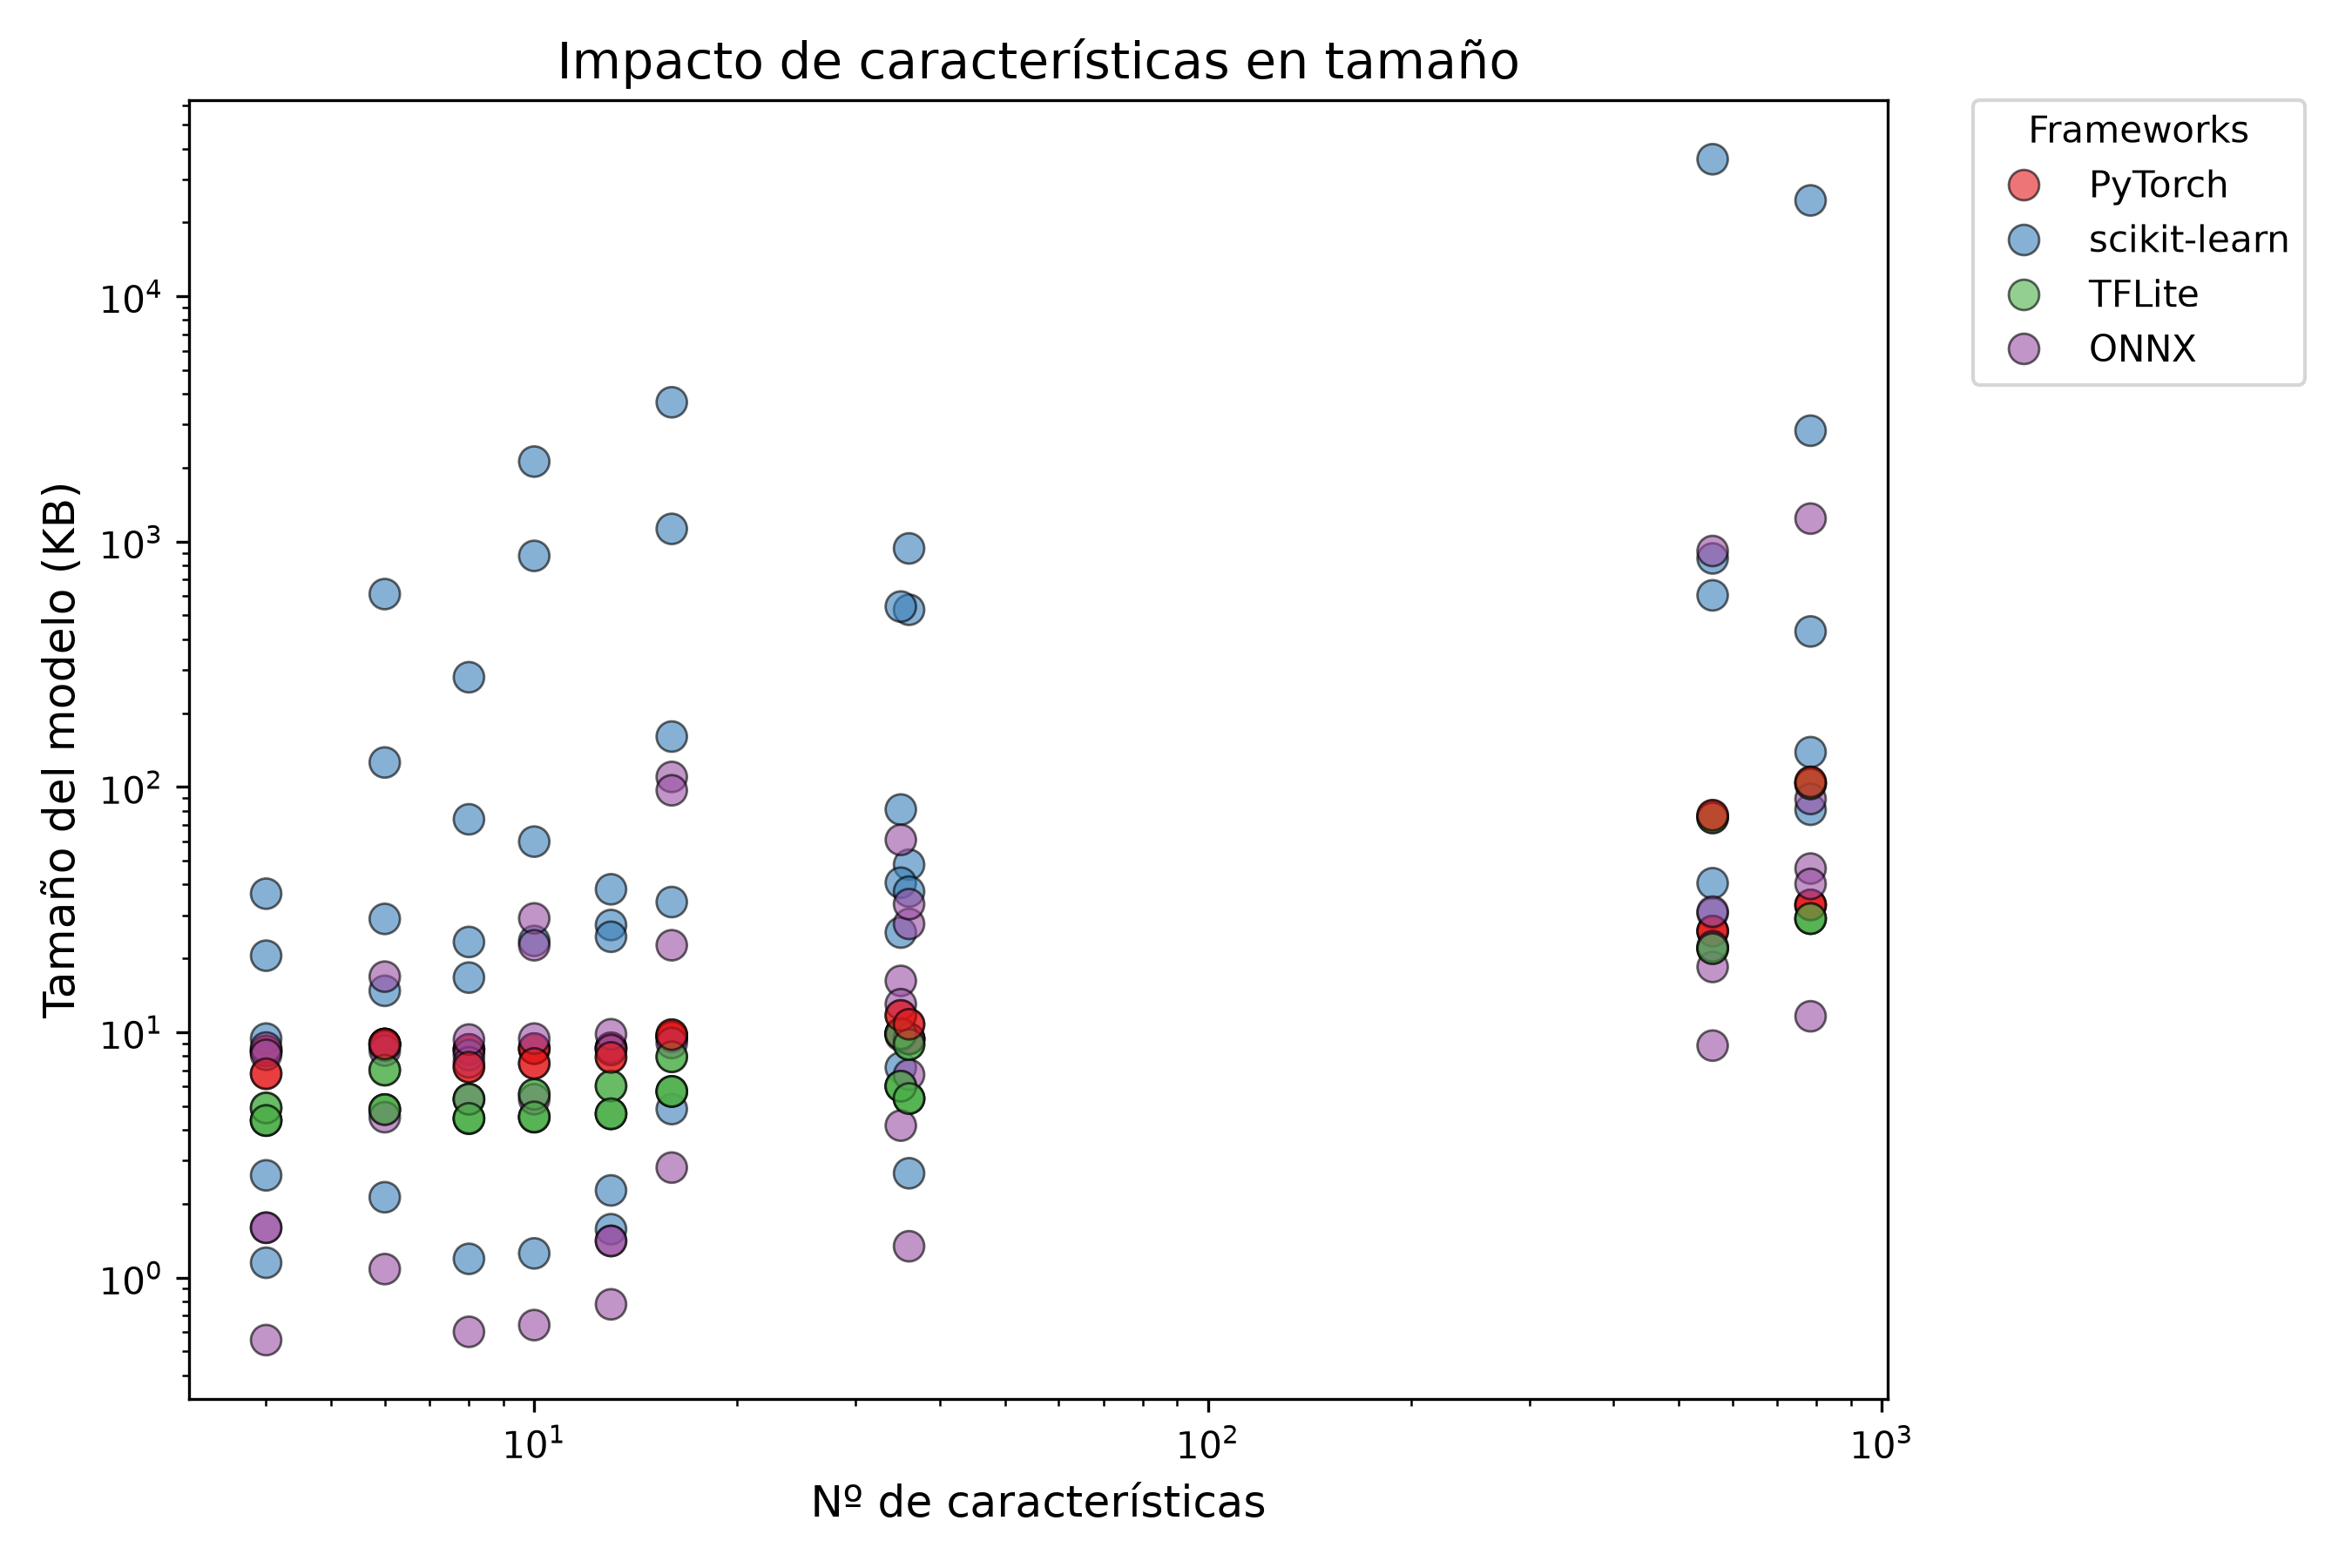
\includegraphics[width=0.728\textwidth]{complexity_features_size_class.png}
    \caption{Relación entre el número de características y el tamaño del modelo por framework en clasificación.}
    \label{fig:features_size_class}
\end{figure}
\vspace{-2em}
\subsubsection{Impacto del número de características en el tamaño del modelo - Regresión}
\begin{figure}[htbp]
    \centering
    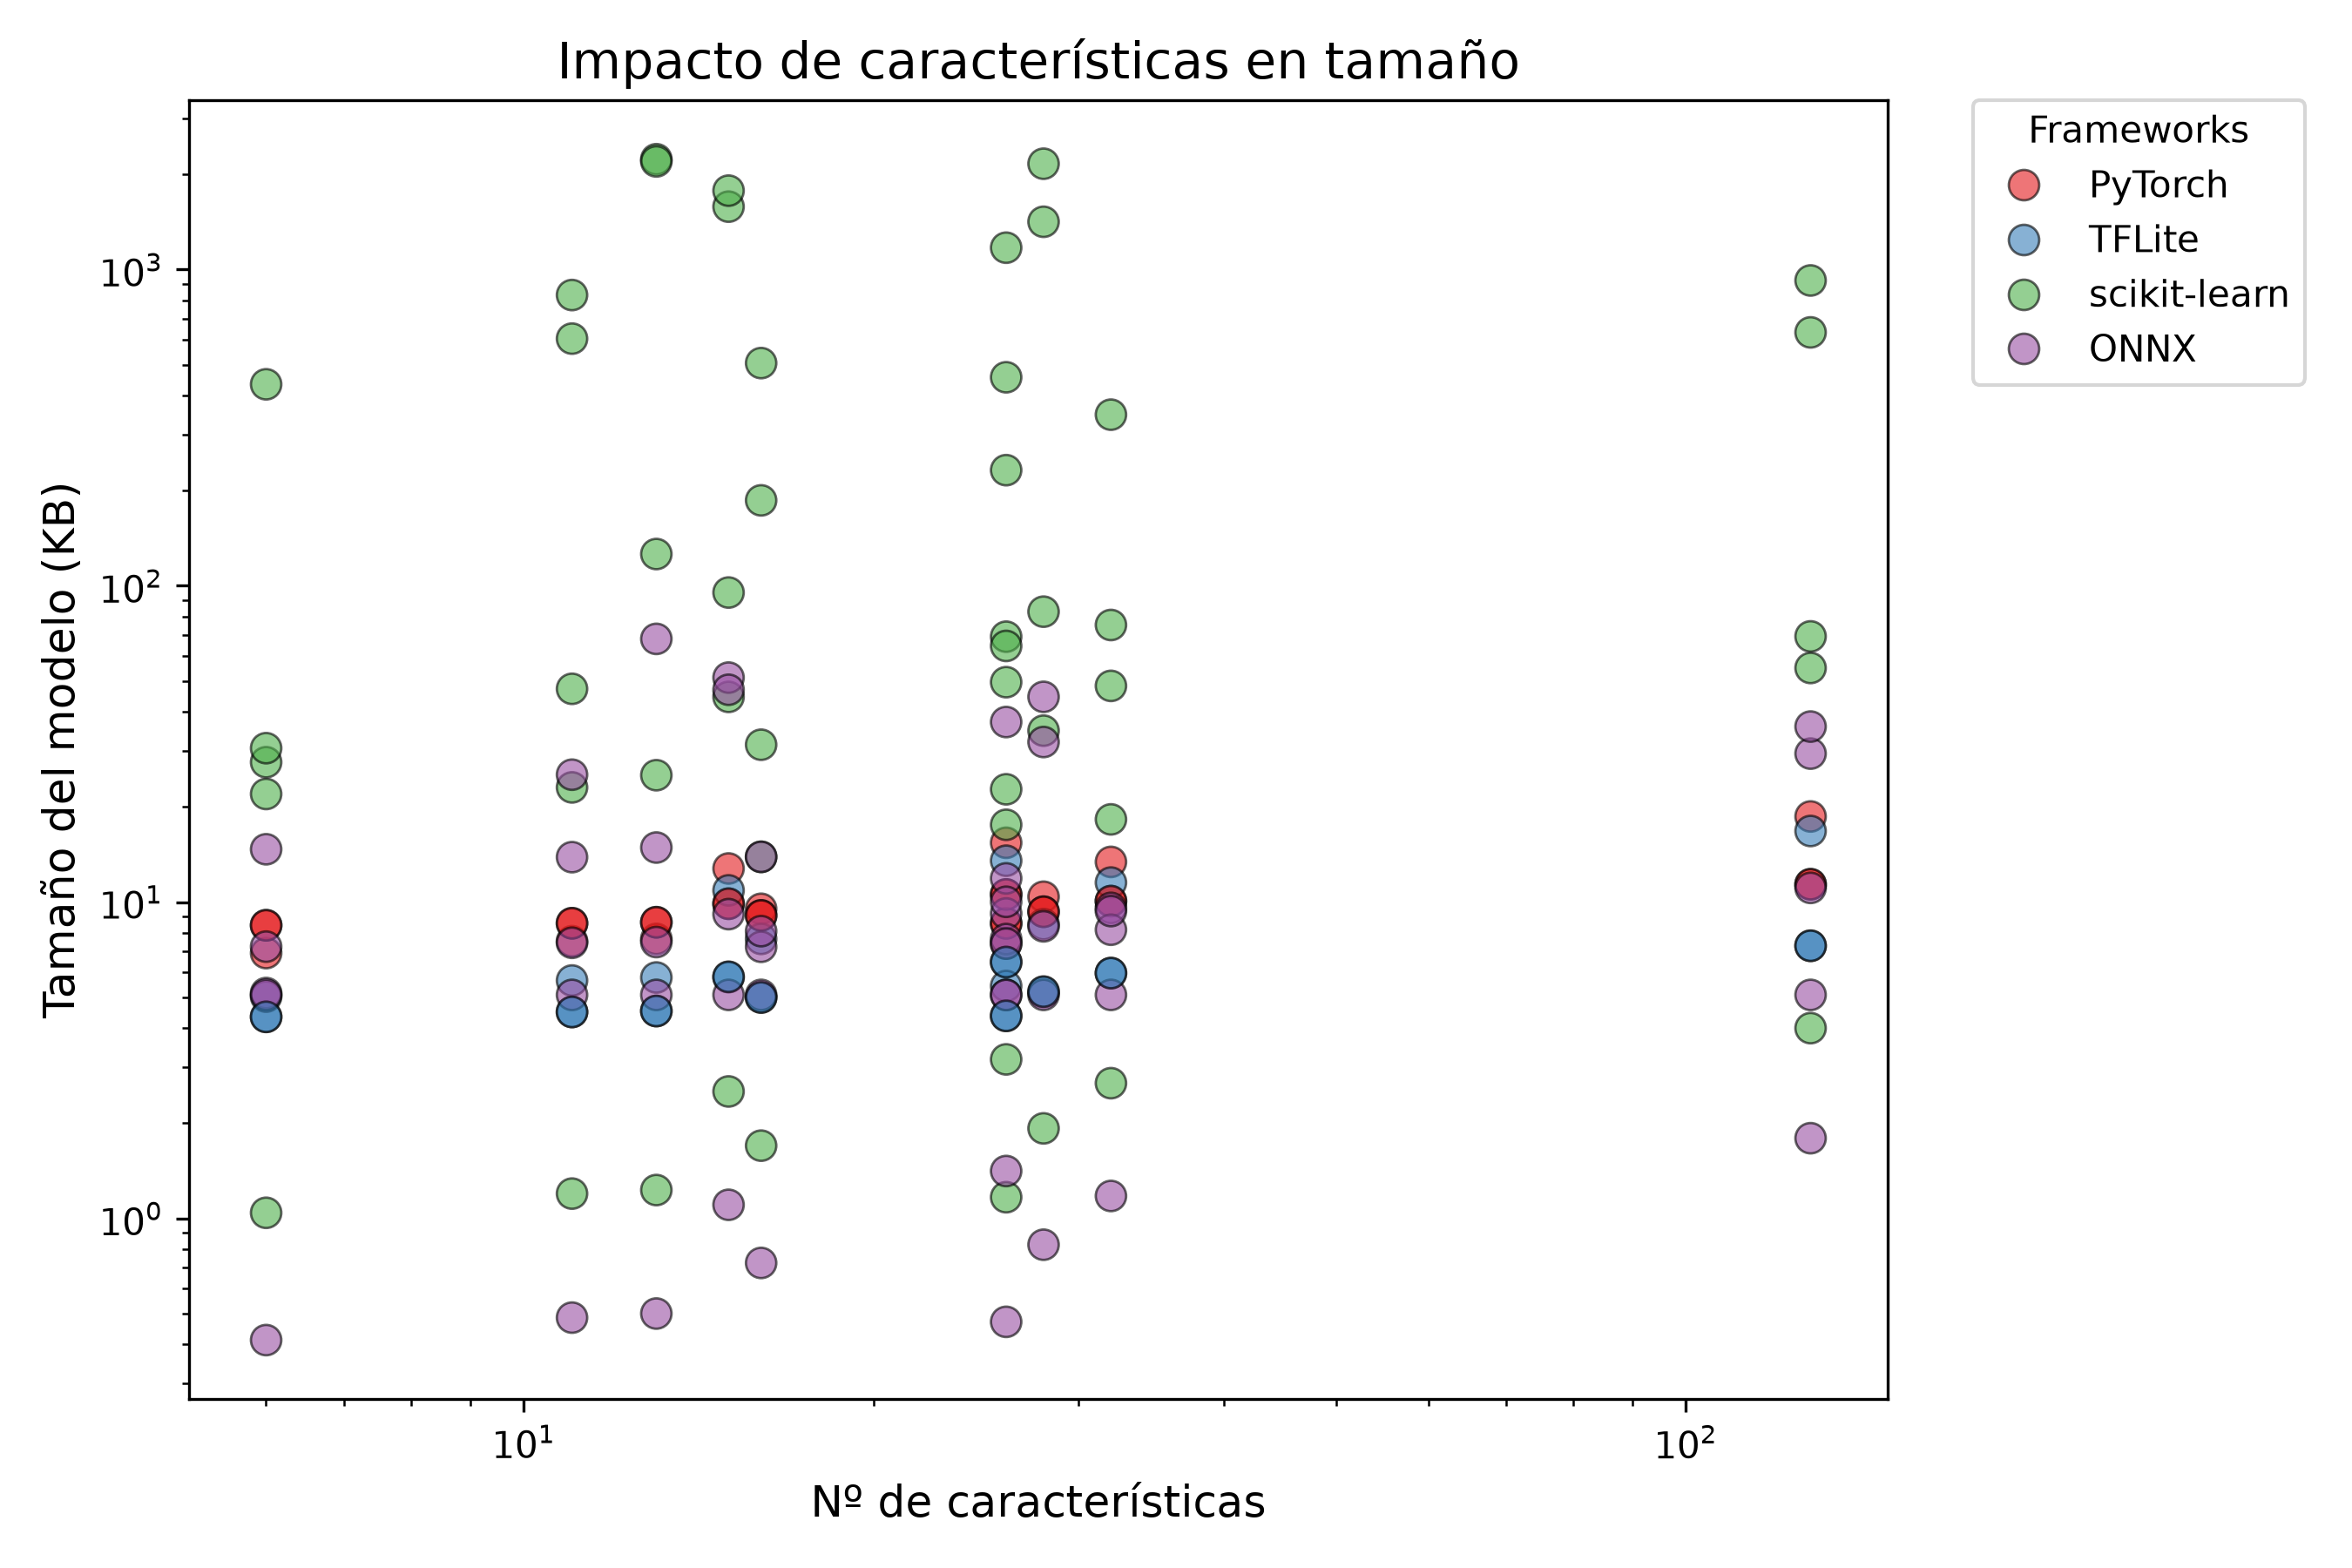
\includegraphics[width=0.728\textwidth]{complexity_features_size_reg.png}
    \caption{Relación entre el número de características y el tamaño del modelo por framework en regresión.}
    \label{fig:features_size_reg}
\end{figure}

El tamaño en disco sí exhibe la tendencia creciente con el número de características que cabría esperar, aunque con
intensidades muy distintas según el algoritmo. Las configuraciones del MLP en PyTorch y TensorFlow Lite muestran un
crecimiento más suave y acotado, de apenas un dígito a dos dígitos de KB entre los datasets de menor y mayor
dimensionalidad, coherente con que solo la primera capa de la red ($I \times H_1$ parámetros) depende directamente del
número de características de entrada. En el extremo opuesto, son algunos de los algoritmos tradicionales los que
muestran el crecimiento más acusado y menos regular. Los puntos que escalan de forma más drástica con la dimensionalidad
corresponden de nuevo a k-NN, cuyo tamaño depende del volumen bruto de datos almacenados, y en menor medida a Random
Forest, cuya complejidad estructural, el número de nodos por árbol, también tiende a crecer en datasets de mayor
dimensionalidad.

\subsubsection{Impacto del número de instancias en la latencia - Clasificación}
\begin{figure}[htbp]
    \centering
    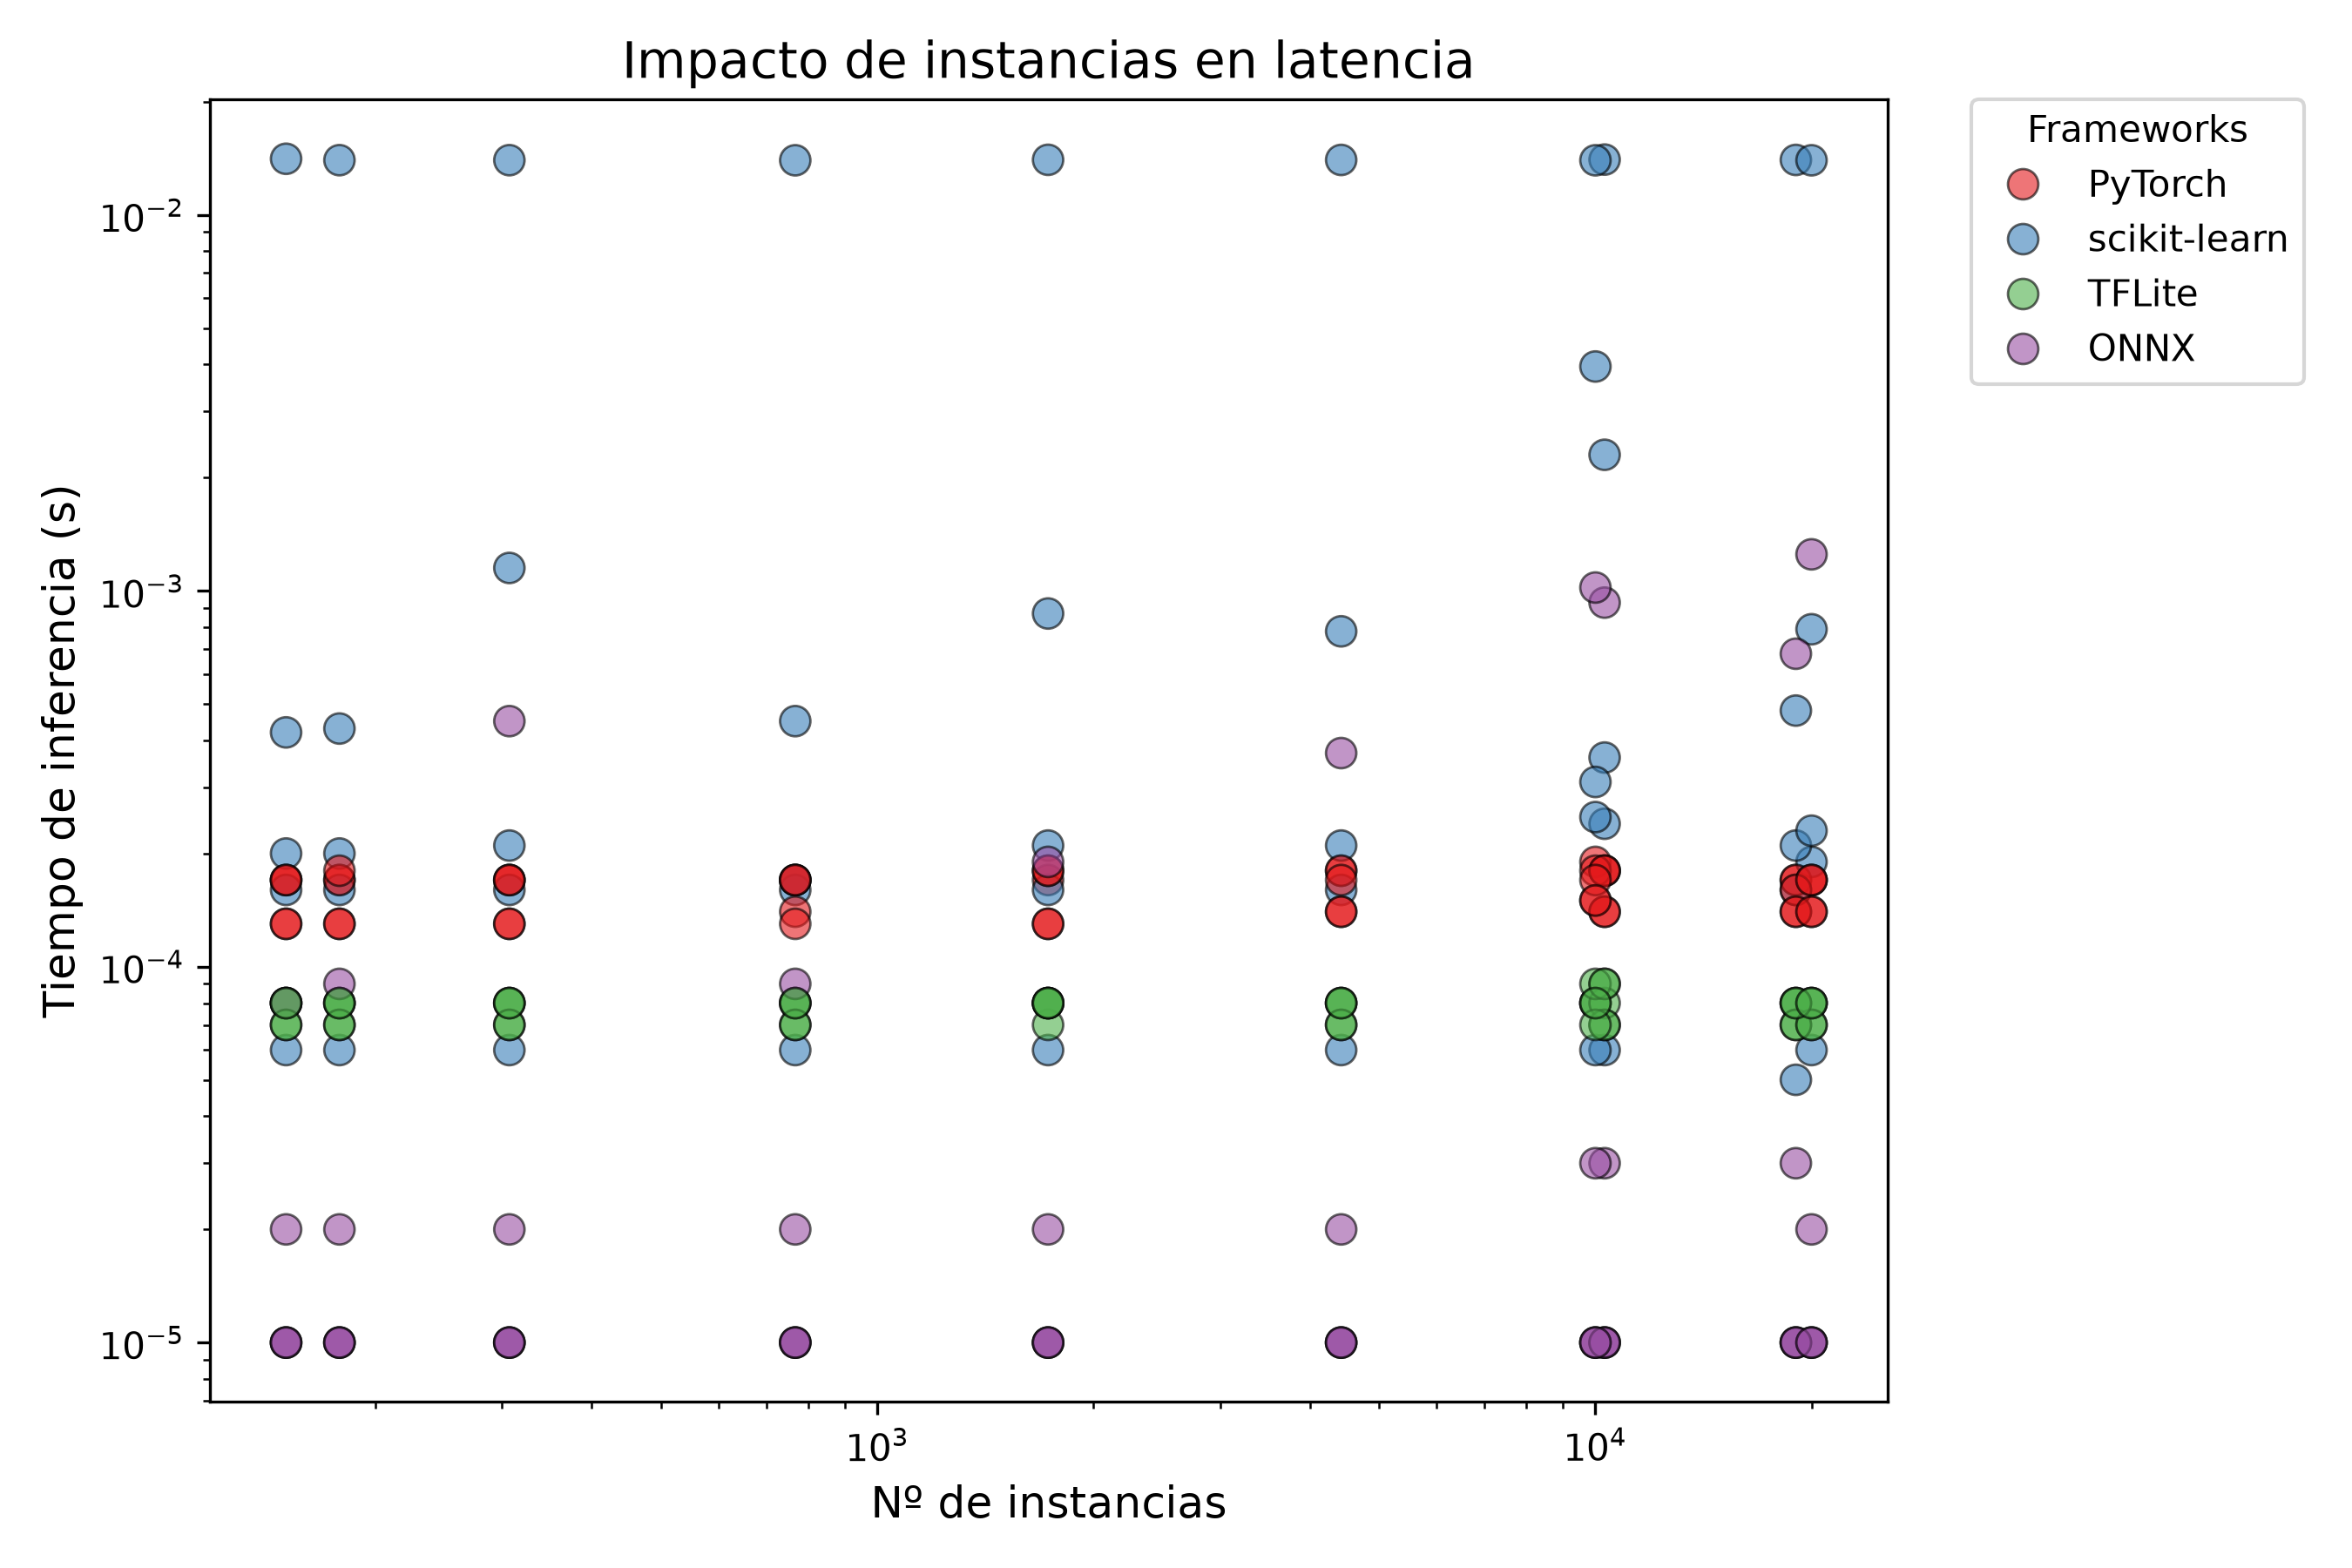
\includegraphics[width=1.0\textwidth]{complexity_instances_latency_class.png}
    \caption{Relación entre el número de instancias y el tiempo de inferencia por framework en clasificación.}
    \label{fig:instances_latency_class}
\end{figure}

\newpage
\subsubsection{Impacto del número de instancias en la latencia - Regresión}
\begin{figure}[htbp]
    \centering
    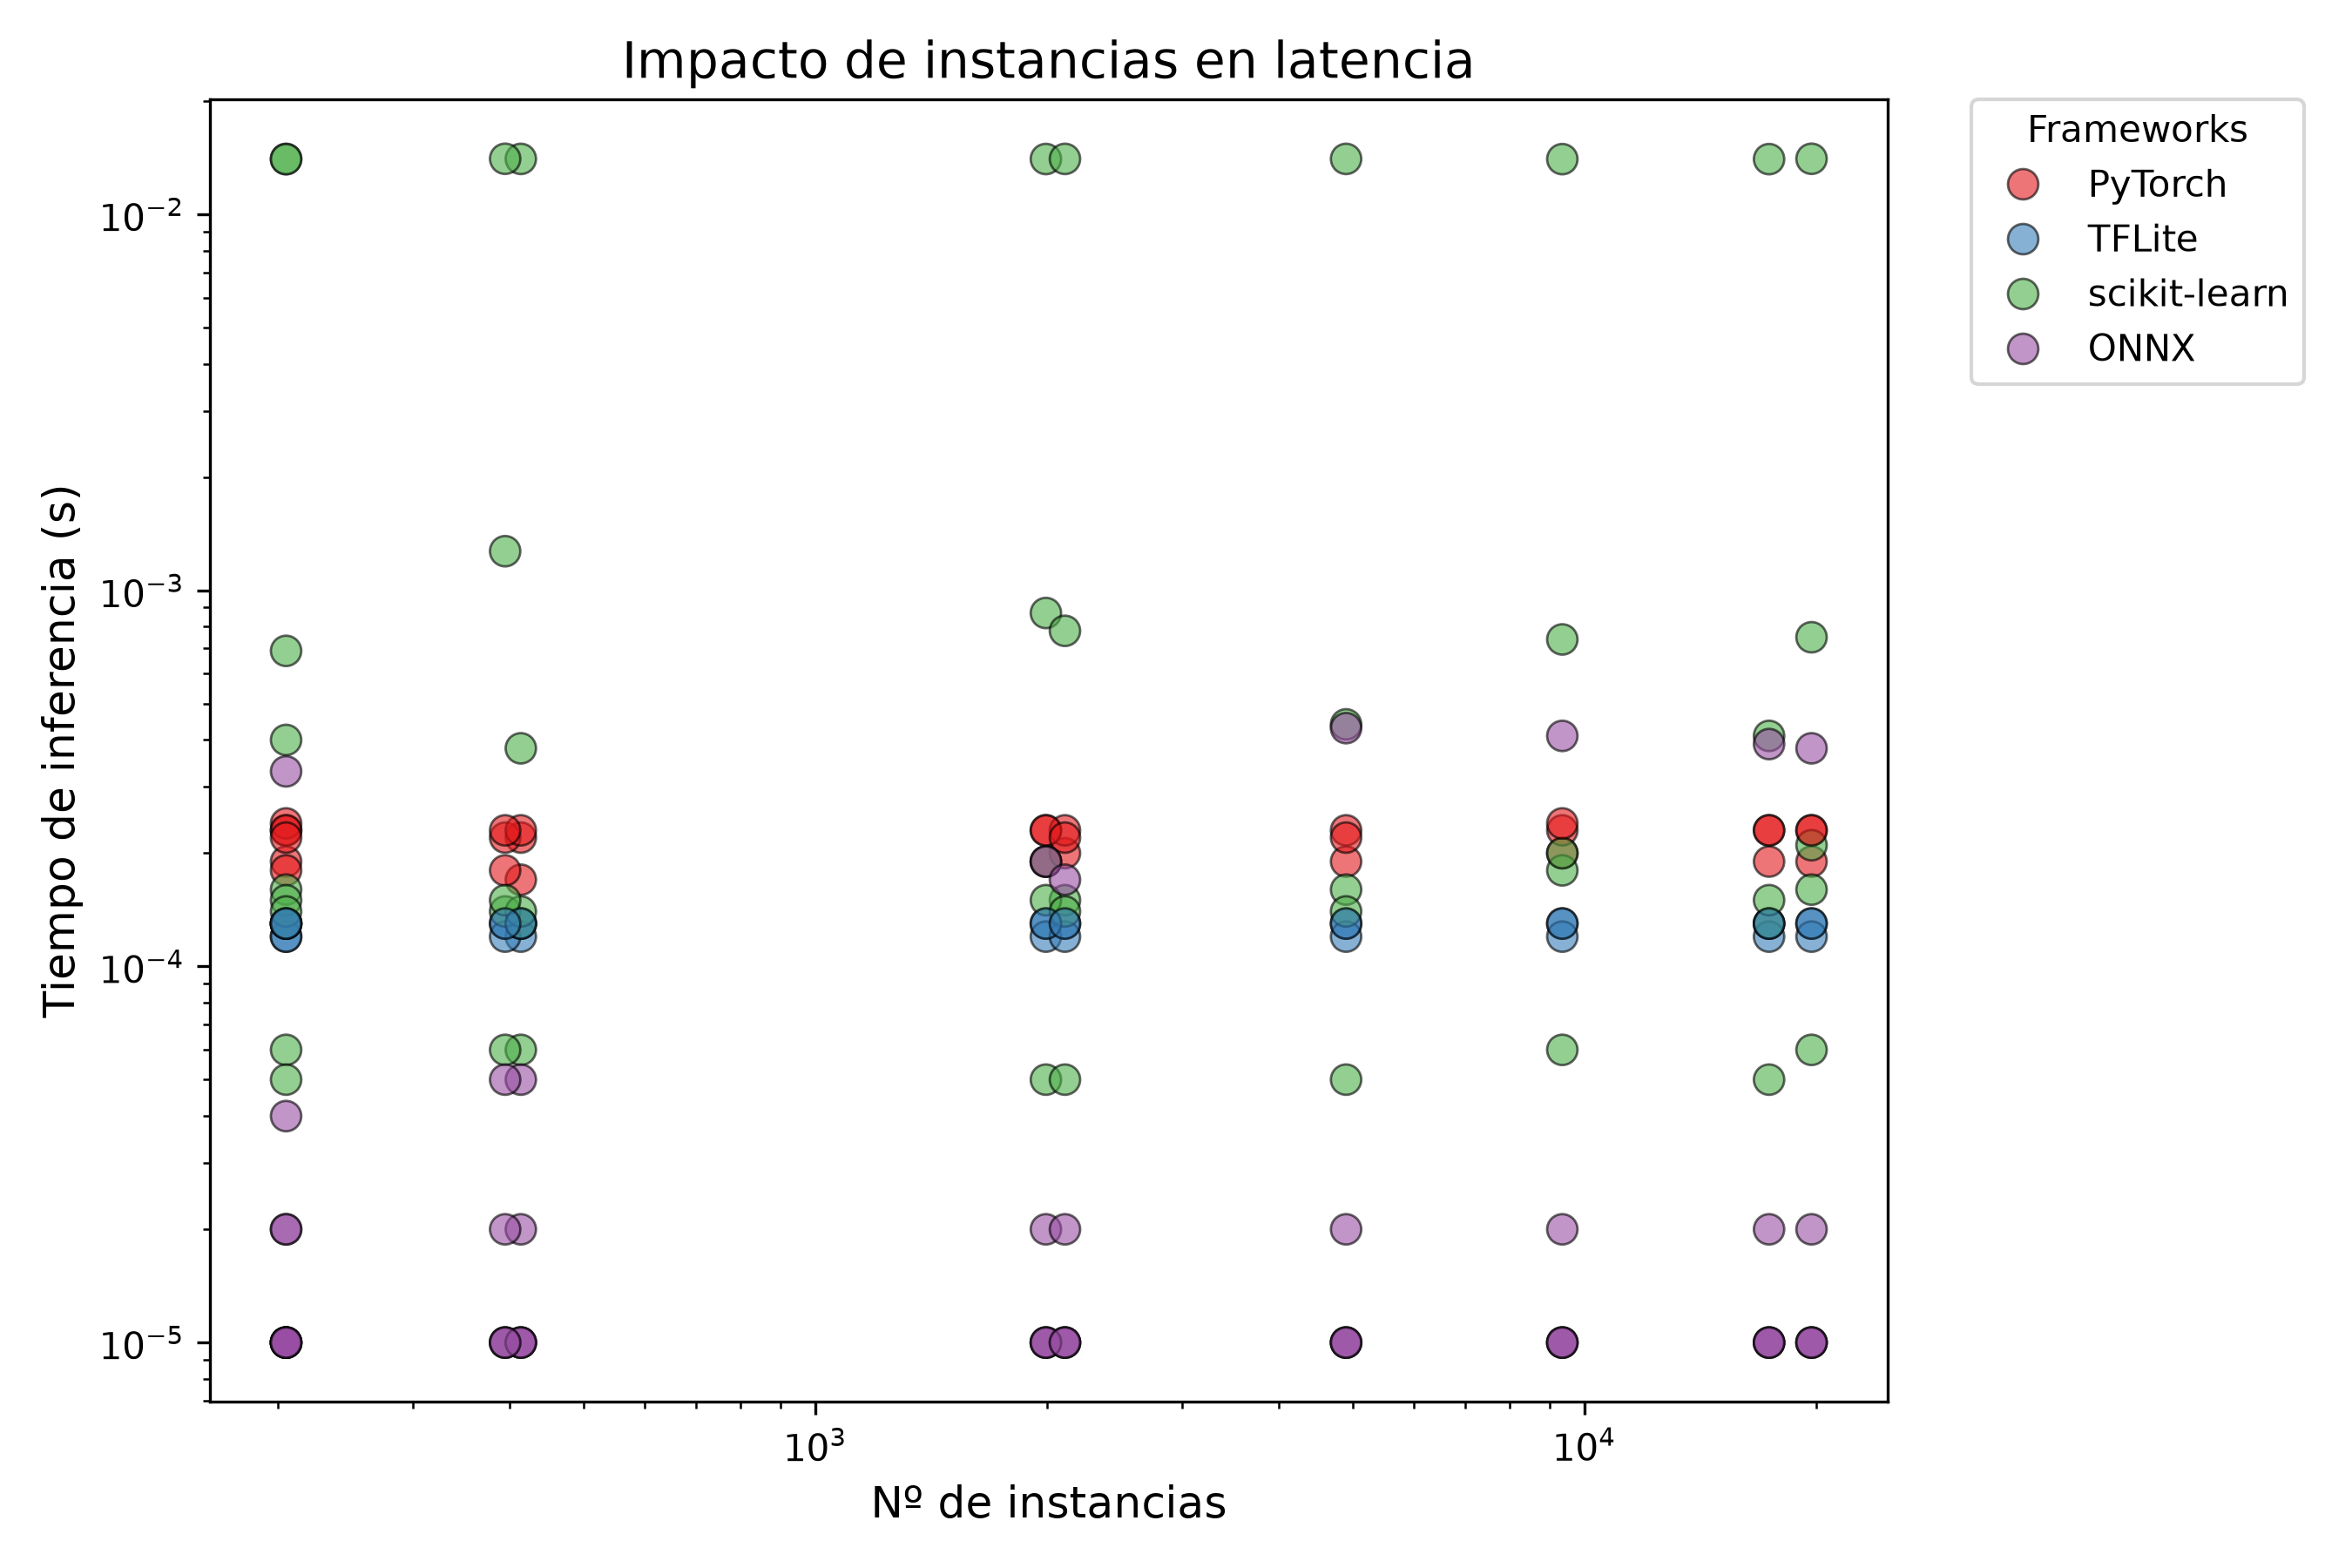
\includegraphics[width=1.0\textwidth]{complexity_instances_latency_reg.png}
    \caption{Relación entre el número de instancias y el tiempo de inferencia por framework en regresión.}
    \label{fig:instances_latency_reg}
\end{figure}

El efecto que tiene el número de instancias sobre la latencia es bastante similar al que se observa con el número de
características. El tiempo de inferencia es prácticamente constante en todos los casos siendo nuevamente una vez más
k-NN el algoritmo que muestra una variación mayor en clasificación, mientras que la regresión muestra una estabilidad
generalizada.

\newpage
\subsubsection{Impacto del número de instancias en el tamaño del modelo- Clasificación}
\begin{figure}[htbp]
    \centering
    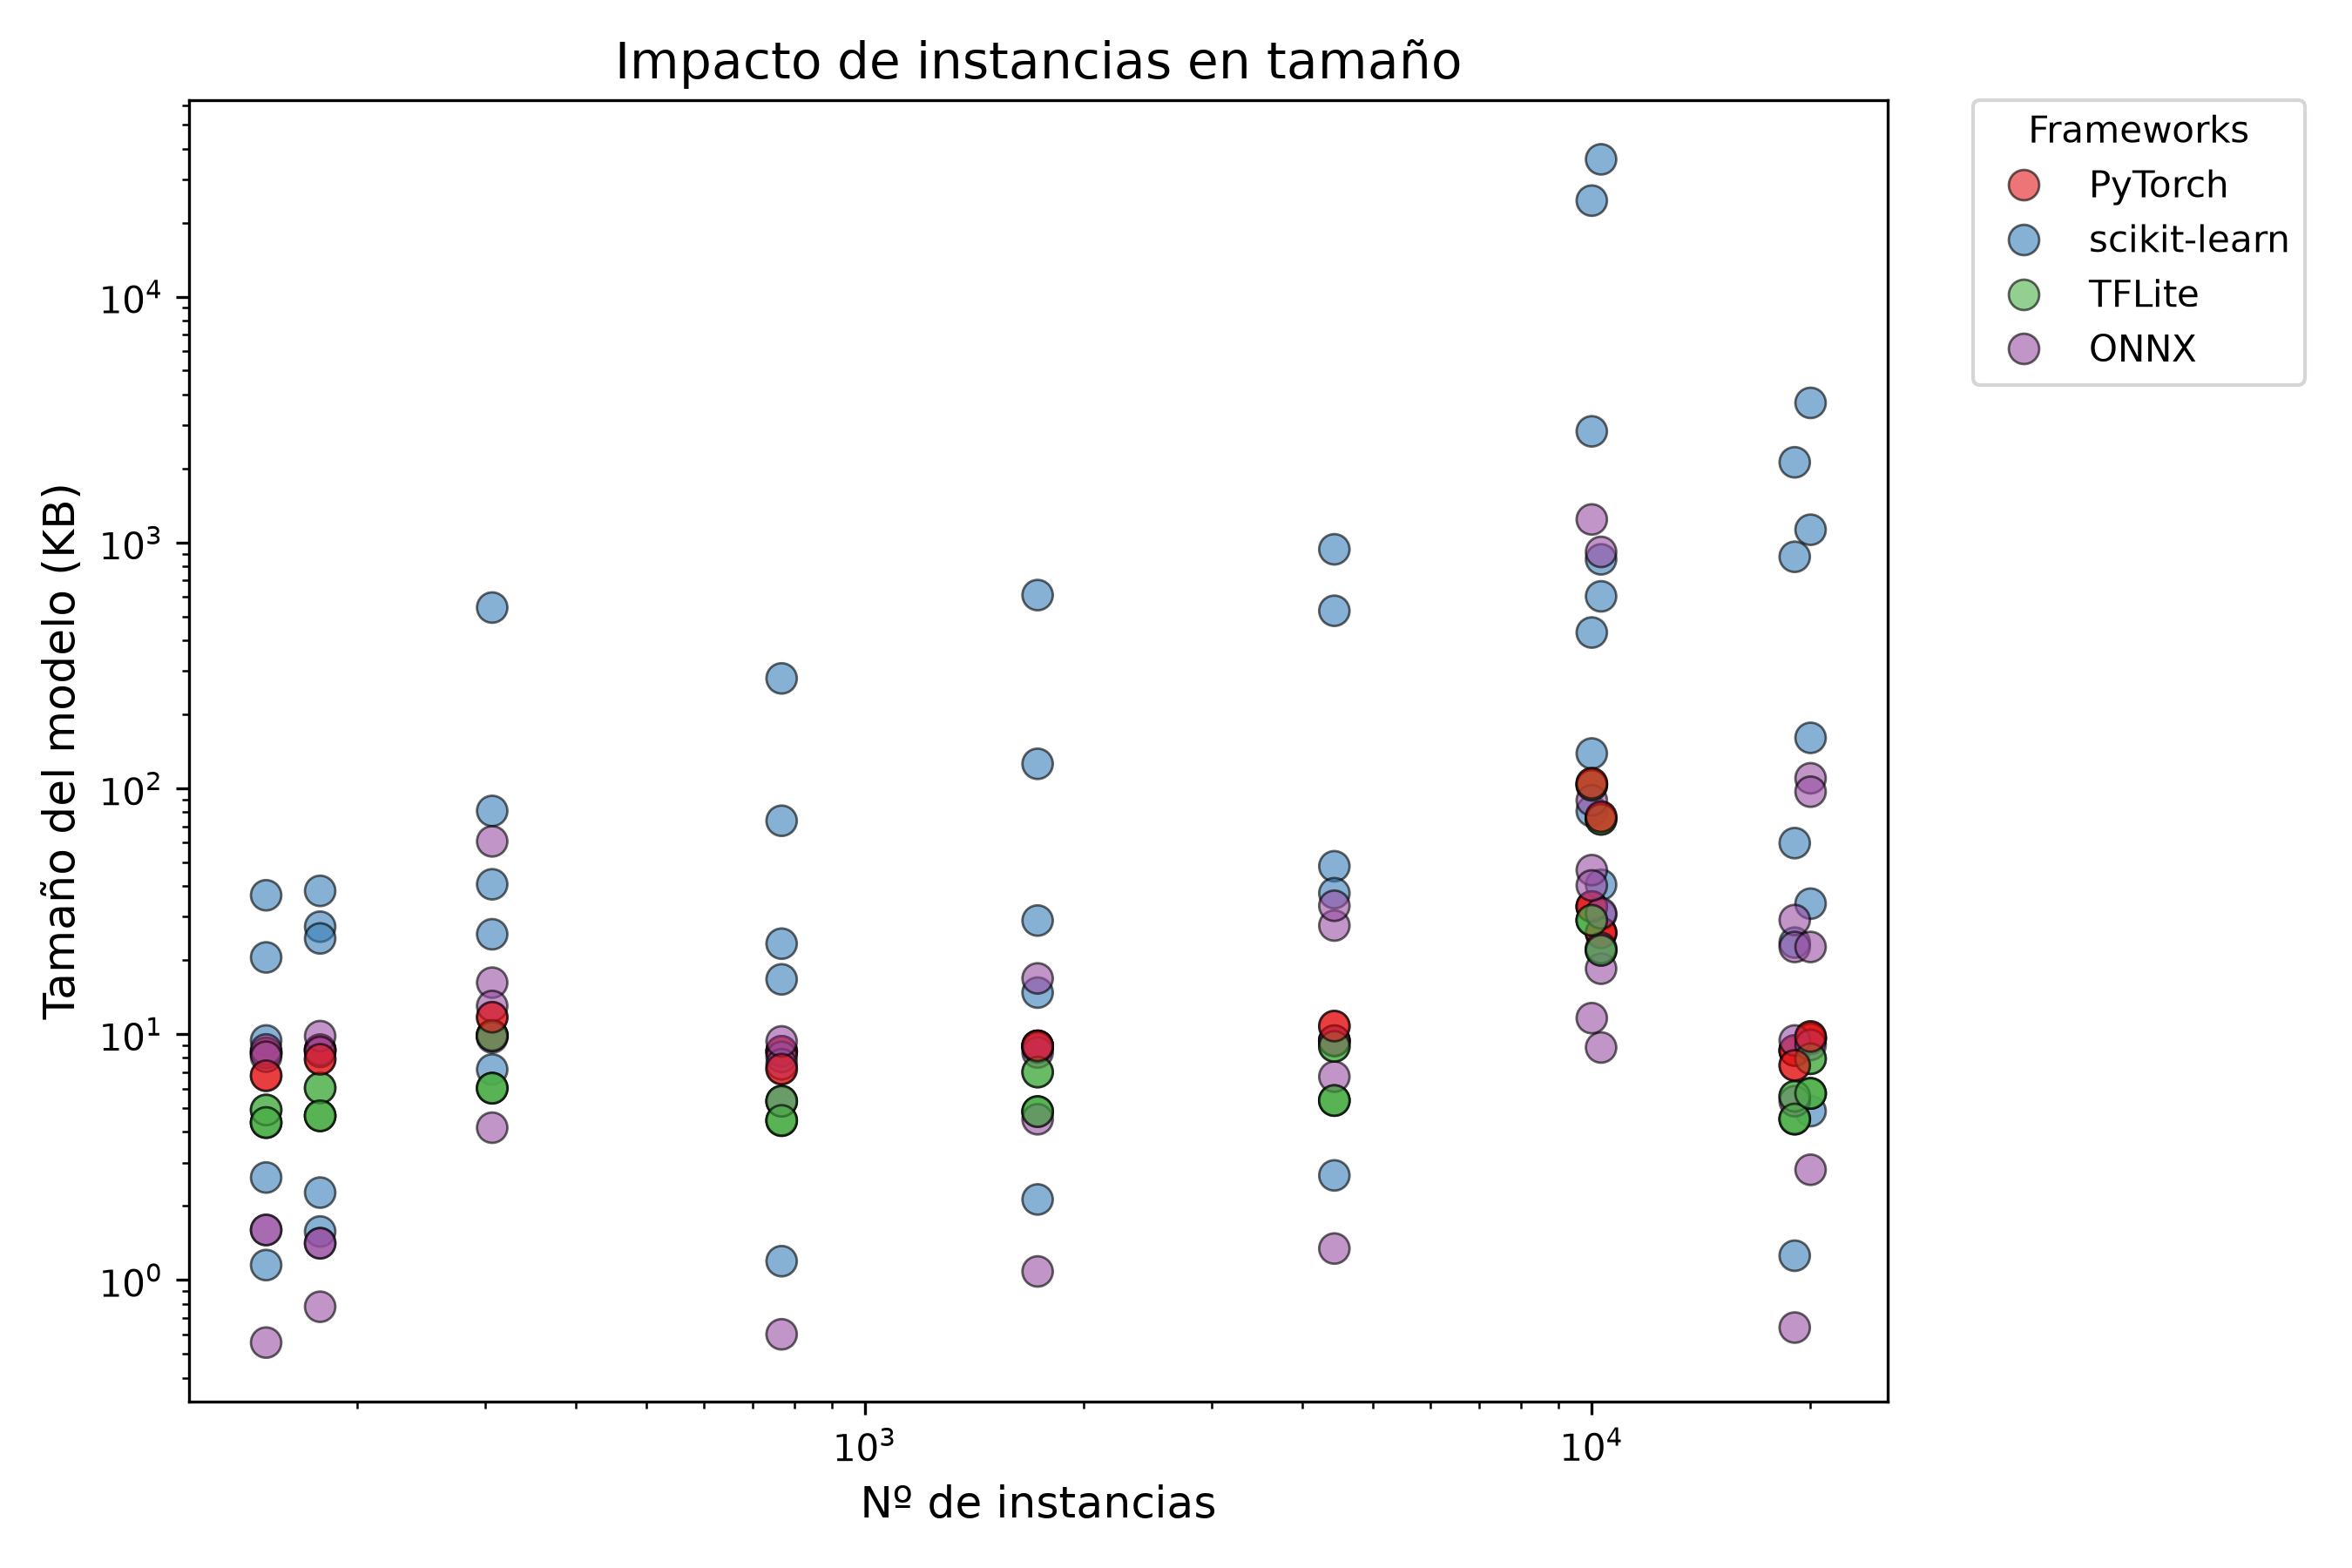
\includegraphics[width=0.728\textwidth]{complexity_instances_size_class.png}
    \caption{Relación entre el número de instancias y el tamaño del modelo por framework en clasificación.}
    \label{fig:instances_size_class}
\end{figure}

\subsubsection{Impacto del número de instancias - Regresión}
\begin{figure}[htbp]
    \centering
    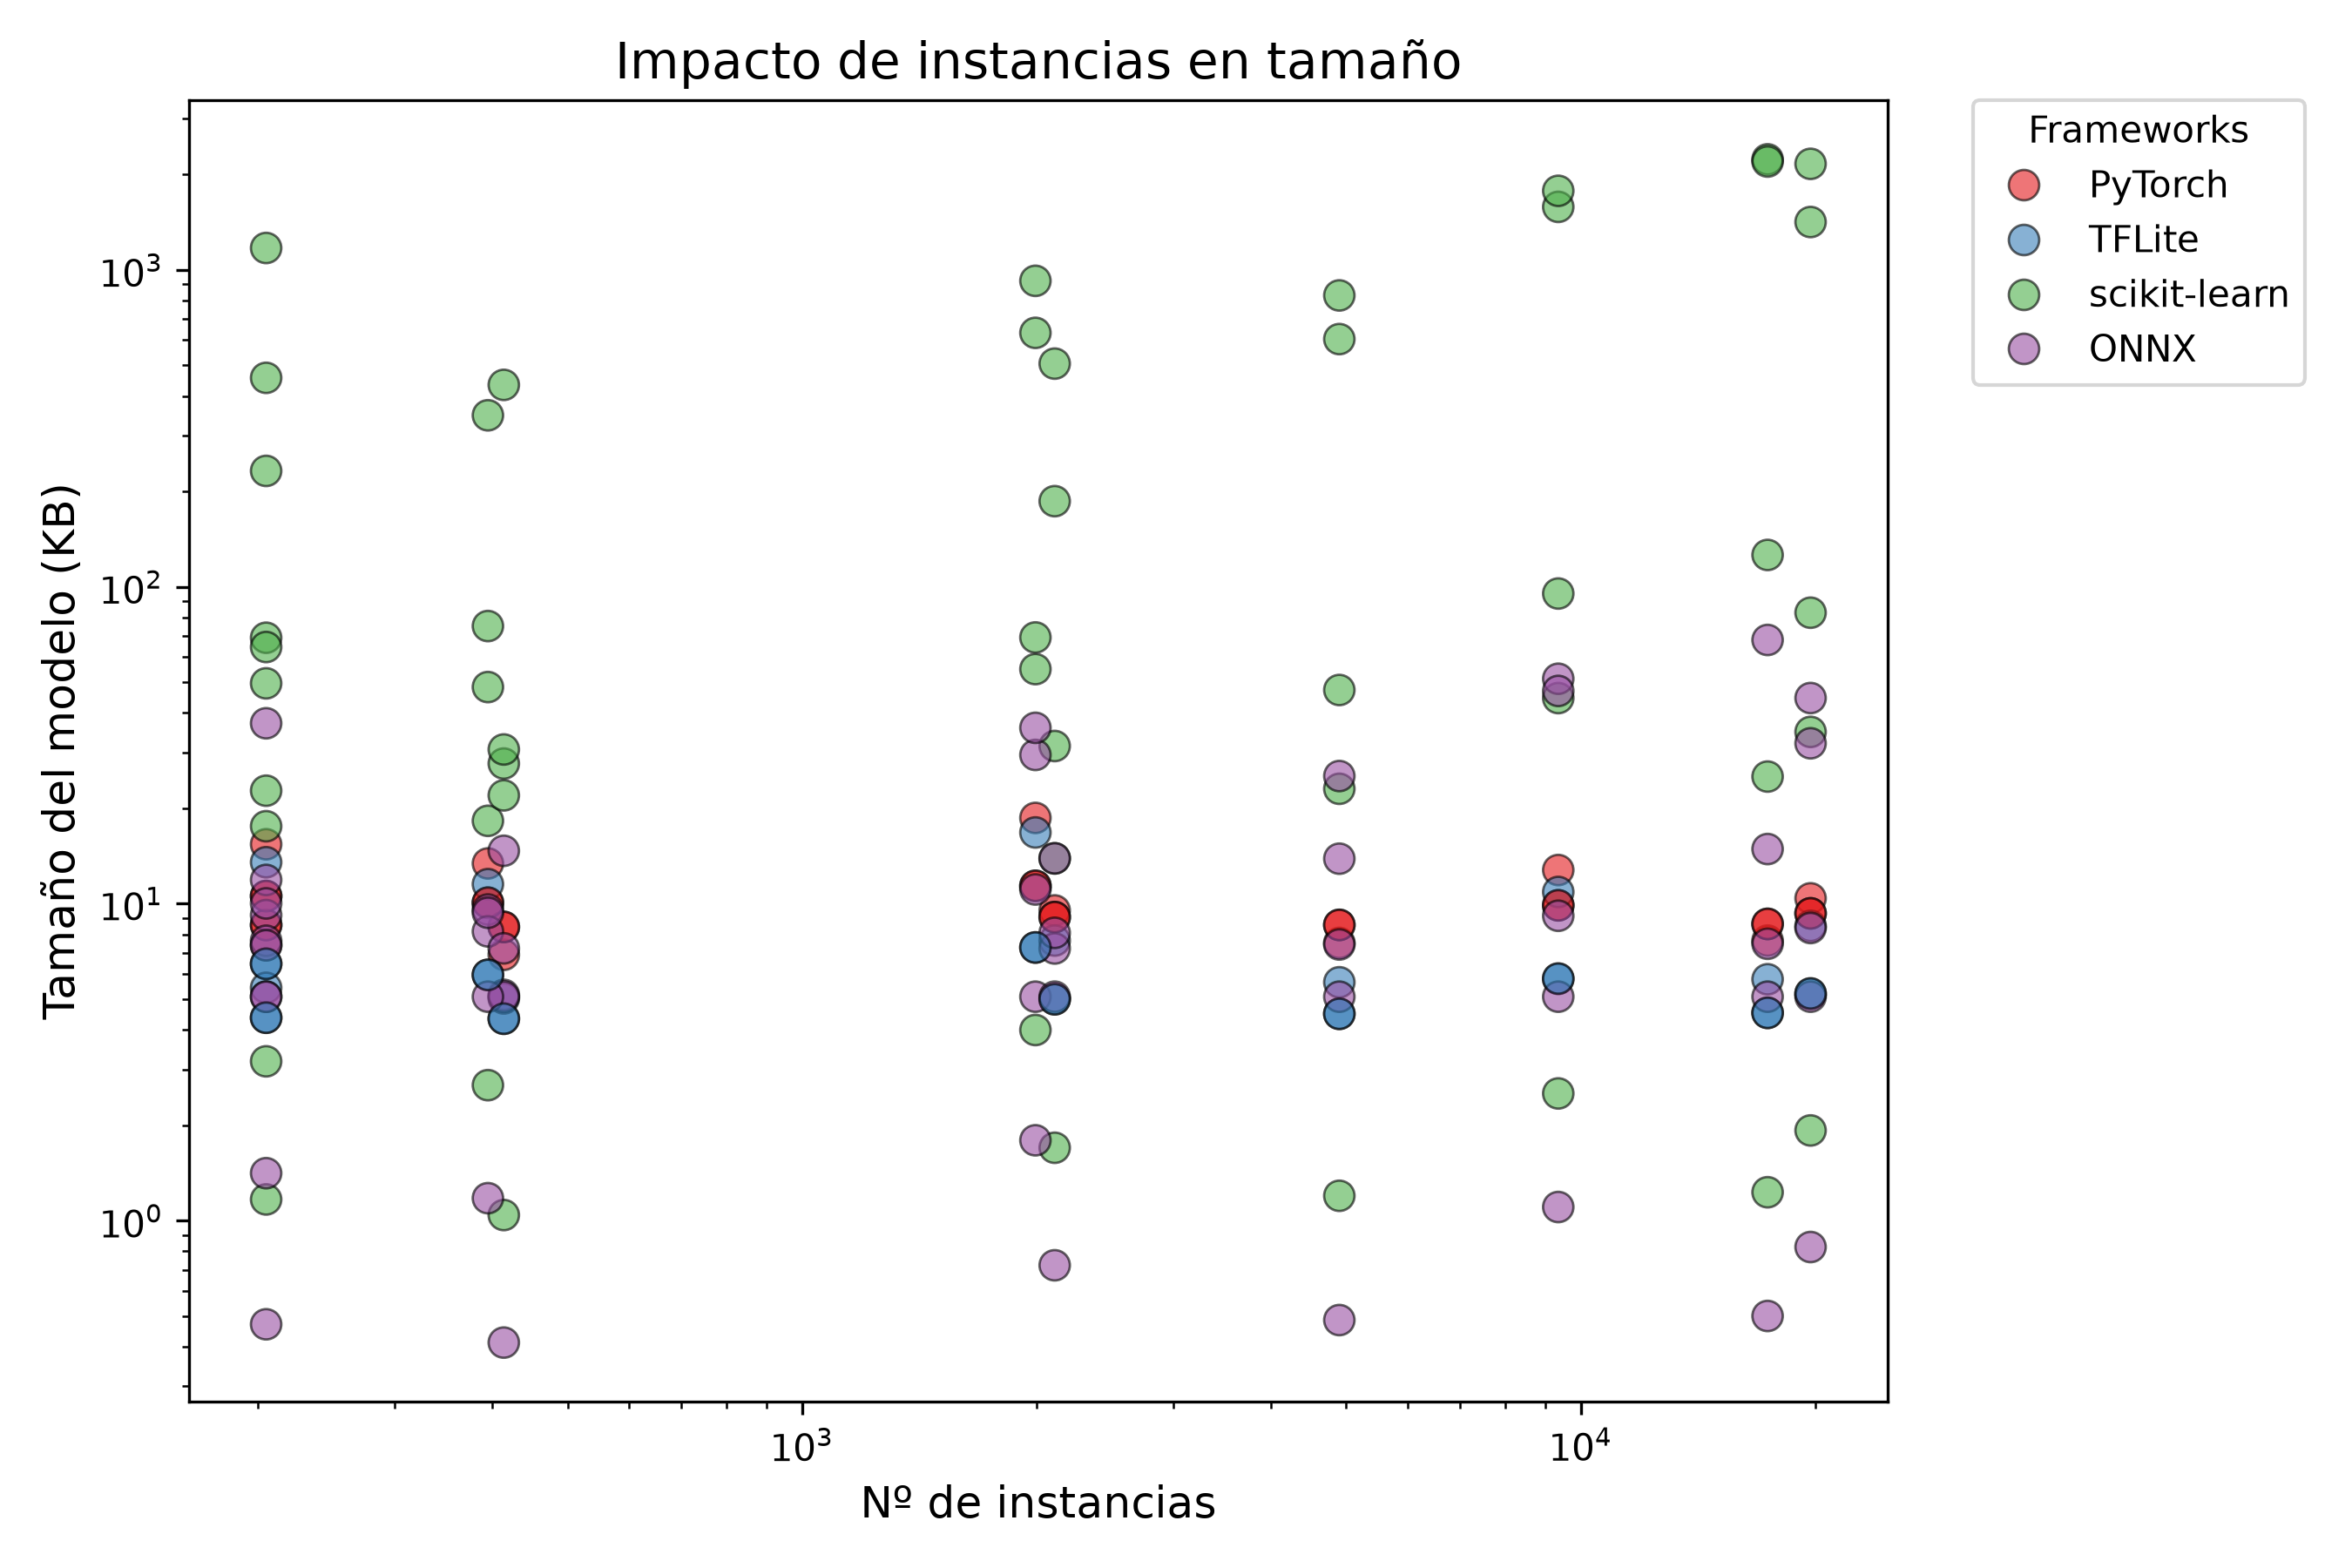
\includegraphics[width=0.728\textwidth]{complexity_instances_size_reg.png}
    \caption{Relación entre el número de instancias y el tamaño del modelo por framework en regresión.}
    \label{fig:instances_size_reg}
\end{figure}

Aunque de forma menos agravada que con el número de características, las instancias también tienen un impacto visible
sobre algunos modelos. Por norma general, los MLP nativos de PyTorch y TensorFlow Lite vuelven a presentarse sólidos
ante la variación del volumen de datos, al contrario que k-NN y, en parte, Random Forest. Pese a que este comportamiento
también se observa en regresión, es más acusado en clasificación. Examinando qué datasets concretos generan los picos
más altos revela un matiz que el propio bloque de resultados no llegaba a precisar: cuando el tamaño del modelo crece,
esto no depende únicamente del número de instancias, sino, aproximadamente, del producto entre instancias y
características, esto es, del volumen total de datos almacenados. Así, Letter Recognition, pese a ser el conjuntos de
datos de clasificación con más instancias (20000), genera modelos considerablemente más ligeros que HAR, solo 10299
instancias pero 561 características, o MNIST, con 10000 instancias y 784 características, precisamente porque su
dimensionalidad (16 características) es muy inferior. Esta observación lleva a deducir que, para un algoritmo de
aprendizaje automático, ambos ejes de escalabilidad, dimensionalidad y volumen, no actúan de forma independiente, sino
conjunta.

\subsection{Proyecciones y extrapolaciones}
Sobre la base de los patrones descritos, esta sección se permite extrapolar, con la cautela propia de toda inferencia
que excede el rango efectivamente observado, dos escenarios de interés práctico para el diseño de futuros sistemas: el
crecimiento del volumen de datos disponible y el uso de arquitecturas más complejas que la empleada en este estudio.
 
\subsubsection{Evolución de la eficiencia al escalar el volumen de datos}
De acuerdo con los patrones establecidos en el apartado anterior, cabría esperar que, si los conjuntos de datos
empleados en este estudio crecieran varios órdenes de magnitud, pasando, por ejemplo, de las decenas de miles de
instancias aquí evaluadas a cientos de miles o millones, el tamaño y la latencia de todos los algoritmos paramétricos
permanecerían esencialmente inalterados, o con un crecimiento moderado, siempre que la arquitectura o los
hiperparámetros de entrenamiento no se modificasen. Sería de esperar que la fase de entrenamiento consumiera más tiempo y
recursos, pero el artefacto final, el que realmente importa para las restricciones de memoria de un microcontrolador, no
vería incrementado su coste de manera exponencial o significativa. La única excepción a esta regla, si se consideran
como opciones para el despliegue en el entorno práctico, modelos como k-NN o Random Forest, sí verían agravados su ya
documentado problema de escalabilidad. Dado que su huella de memoria crece con la dimensionalidad y volumen del problema,
un crecimiento sostenido de los mismos terminaría por hacerlos completamente inviables para cualquier plataforma con
restricciones de memoria, incluso con las técnicas de reducción de aplicadas en la fase de exportación a ONNX, que
mitigan el problema pero no lo eliminan estructuralmente.
 
\subsubsection{Efecto de una arquitectura MLP más compleja sobre el tamaño del modelo}
Dado que el MLP sería el modelo preferido para el despliegue en microcontroladores, según lo observado en el frente de
Pareto, conviene analizar cómo se vería afectado su tamaño en disco si se optase por una arquitectura más profunda o más
ancha que la empleada en este estudio. Para razonar sobre este escenario resulta útil recurrir al conteo de parámetros
de un perceptrón multicapa con dos capas ocultas de anchos $H_1$ y $H_2$, dimensión de entrada $I$ y dimensión de salida
$O$:
\[
P(I, H_1, H_2, O) = \underbrace{I \cdot H_1 + H_1}_{\text{capa oculta 1}} + 
\underbrace{H_1 \cdot H_2 + H_2}_{\text{capa oculta 2}} + \underbrace{H_2 \cdot O + O}_{\text{capa de salida}}
\]

Para la arquitectura empleada en este trabajo ($H_1=32$, $H_2=26$), esta expresión se reduce a $P = 32I + 27O + 890$. La
observación clave de esta fórmula es que sus tres términos no escalan de la misma manera ante un incremento de la
complejidad del problema. Si se amplía el número de características de entrada $I$, el eje de escalabilidad estudiado en
el apartado anterior, el crecimiento del número de parámetros es lineal, gobernado únicamente por el ancho de la primera
capa oculta ($H_1$). Sin embargo, si se optase por una arquitectura más profunda o más ancha, por ejemplo, doblando
ambos anchos ocultos a $H_1=64$, $H_2=52$, el término dominante, $H_1 \cdot H_2$, pasaría de $832$ a $3328$ parámetros:
un crecimiento cuadrático, cuatro veces superior al que produciría duplicar el número de características de entrada. En
otras palabras, el tamaño del modelo es mucho más sensible a la profundidad/anchura de la red que a la dimensionalidad
de los datos que procesa.\\
 
En cuanto al factor de reducción aplicable a dicha arquitectura ampliada, conviene una lectura prudente de la cifra de
compresión del $\sim 92.8\%$ documentada para TensorFlow Lite cuantizado frente al modelo base de scikit-learn en
clasificación. Dicho porcentaje supera el techo teórico que cabría esperar de la cuantización numérica en solitario:
pasar de coma flotante a enteros de 8 bits suele suponer una reducción del $75\%$--$80\%$ sobre el tamaño bruto de los
tensores de pesos. Que la reducción observada sea superior a ese límite sugiere que una parte no despreciable del ahorro
actual no proviene de la cuantización en sí, sino de eliminar la sobrecarga fija de serialización del ecosistema Python
(\path{pickle}/\path{joblib}), que, para una red tan compacta como la aquí empleada, representa una fracción
significativa del tamaño total del archivo. Esta sobrecarga es, precisamente, constante y no escala con el número de
parámetros del modelo. Por consiguiente, cabría esperar que, al aplicar las mismas técnicas de cuantización a una
arquitectura sensiblemente más compleja, el peso relativo de dicha sobrecarga fija se diluyese frente al de los tensores
de pesos, ahora mucho más voluminosos, y que el porcentaje de reducción alcanzable convergiese progresivamente hacia el
límite teórico del $75\%$--$80\%$ propio de la cuantización numérica. Esto no implica en absoluto que la cuantización
pierda utilidad al escalar la arquitectura, sino todo lo contrario. El ahorro en KB absolutos seguiría siendo, de hecho,
mayor cuantos más parámetros hubiera que comprimir. De este modo, el porcentaje de reducción reportado en este estudio
debe entenderse como una cota optimista, particularmente favorable por tratarse de una red de reducidas dimensiones, y
no como una constante universal extrapolable sin matices a cualquier topología de red.


\chapter{Conclusiones y recomendaciones}
El presente trabajo partía de una pregunta con vocación práctica: dada la creciente demanda de inteligencia artificial
en dispositivos con recursos extremadamente limitados, ¿qué combinación de framework, técnica de compresión y algoritmo
ofrece el mejor compromiso entre rendimiento predictivo, tamaño y latencia? Para responderla, se ha diseñado y
ejecutado un banco de pruebas experimental que evalúa, bajo un protocolo común y reproducible, cinco algoritmos de
aprendizaje automático clásico y una arquitectura de perceptrón multicapa, desplegados a través de cuatro rutas de
implementación (scikit-learn nativo, ONNX, PyTorch y TensorFlow Lite), combinadas con cuantización post-entrenamiento y
destilación de conocimiento, diez conjuntos de datos de clasificación y diez de regresión, procedentes de dominios tan
dispares como la salud, la automoción, la astrofísica o la sociología. Este capítulo cierra el trabajo sintetizando los
hallazgos obtenidos en el capítulo de resultados, discutiendo sus implicaciones prácticas para el diseño de sistemas
TinyML y proponiendo líneas de continuación para investigaciones futuras.
 
\section{Síntesis de los resultados principales}
A lo largo del capítulo anterior se han acumulado una gran cantidad de observaciones puntuales, respaldadas por
tablas descriptivas y por el contraste inferencial de Friedman y Nemenyi. Corresponde ahora destilar estas
observaciones en un conjunto reducido de hallazgos generales, organizados en torno a las preguntas de investigación
formuladas en el capítulo \autoref{chap:objetivos}: Formulación del problema y objetivos.
 
\subsection{El framework de despliegue condiciona tanto el rendimiento como el coste}
El hallazgo más transversal del trabajo es que la elección del motor de inferencia no es una decisión neutra desde el
punto de vista predictivo, contrariamente a lo que cabría esperar si se asumiera que todo motor de cuantización a
INT8 aplica esencialmente la misma transformación matemática. Los resultados demuestran justo lo contrario: existe
una brecha entre los frameworks que cuentan con un calibrador de cuantización propio y ajustado a su arquitectura,
como PyTorch, mediante FX Graph Mode, y TensorFlow Lite, mediante su conversor nativo, y la exportación genérica a
través de ONNX. Esta misma brecha se observa, de forma aún más acusada, en el tamaño y la latencia: TensorFlow Lite,
gracias a su serialización mediante \textit{FlatBuffers}, se consolida como el formato más compacto del estudio en
prácticamente todos los escenarios evaluados, mientras que PyTorch, pese a ofrecer con frecuencia el mejor techo
predictivo, arrastra durante todo el trabajo una penalización de latencia achacable a la sobrecarga de instanciación
dinámica de tensores y al despacho del intérprete de TorchScript en inferencias unitarias. En definitiva, no existe un
framework universalmente superior, sino un compromiso explícito entre capacidad predictiva (PyTorch), eficiencia de
almacenamiento y velocidad (TensorFlow Lite) e interoperabilidad sin necesidad de reentrenar (ONNX), cuyo peso relativo
depende de la prioridad del proyecto.
 
\subsection{La cuantización y la destilación de conocimiento no son técnicas intercambiables}
El estudio permite además distinguir con claridad el papel funcional de cada técnica de compresión, algo que rara vez
se aborda de forma aislada en la literatura consultada en el \autoref{chapt_estado_tecnica}: Estado de la técnica. La
cuantización post-entrenamiento reduce el tamaño, pero lo hace a costa de una cierta degradación predictiva, que es
mayor cuanto menos maduro es el calibrador del framework. La destilación de conocimiento, por el contrario, se ha
revelado como una técnica prácticamente sin contrapartidas dentro del alcance de este trabajo: al operar exclusivamente
sobre la función de pérdida durante el entrenamiento, no introduce ningún coste adicional de tamaño ni de latencia en el
modelo desplegado, mientras que en la inmensa mayoría de los casos evaluados iguala o supera el rendimiento del modelo
original, incluso cuando el estudiante conserva una arquitectura mucho más ligera que el profesor. Esta observación
coincide con lo apuntado en la literatura sobre destilación~\cite{gou2021ijcv}. La combinación de cuantización y
destilación no solo es viable, sino que, por ejemplo, en TensorFlow permite recuperar una parte sustancial del
rendimiento perdido por la cuantización pura. En cuanto al hiperparámetro de temperatura, la configuración $T=2$ superó
de forma consistente a $T=1$, o lo que es lo mismo, no usarla, en todos los escenarios de clasificación evaluados,
confirmando empíricamente el efecto beneficioso del suavizado de las distribuciones del profesor descrito en la
literatura~\cite{xu2023ieecomst}.
 
\subsection{Clasificación y regresión no se comportan igual ante la compresión}
Uno de los hallazgos más relevantes desde el punto de vista metodológico, y que justifica a posteriori la decisión de
incluir ambas tareas en el mismo protocolo experimental, es que las técnicas de compresión no son igualmente seguras en
clasificación y en regresión. El caso más extremo es el colapso del MLP cuantizado mediante ONNX en regresión, cuyo
coeficiente de determinación medio se desploma a valores negativos, frente a una degradación mucho más contenida en
clasificación. La explicación reside en la naturaleza de la capa de salida: en clasificación, la función de activación
acotada (softmax o sigmoide) actúa como un amortiguador natural frente al ruido de cuantización, mientras que en
regresión la salida continua y no acotada carece de ese margen de seguridad, de modo que cualquier error de escala se
propaga directamente al valor predicho. Este mismo patrón, aunque de forma menos dramática, se observa en TensorFlow,
cuya política de cuantización estricta a \path{tf.int8} produce recortes de rango notable en datasets de alta varianza.
PyTorch, por el contrario, demuestra en este trabajo ser el framework más seguro para cuantizar modelos de regresión,
gracias a la protección de escala que ofrece su calibrador FX Graph Mode. La implicación práctica es clara: las
recomendaciones de compresión que funcionan bien en clasificación no pueden extrapolarse sin más a la regresión, y
cualquier proyecto orientado a estimar magnitudes continuas debe validar explícitamente el comportamiento del
calibrador de cuantización elegido antes de darlo por bueno.
 
\subsection{Ningún modelo domina en solitario: la frontera de Pareto y la escalabilidad}
El análisis multiobjetivo desarrollado en el bloque final de resultados confirma, con datos, la intuición que motivó
todo el trabajo: no existe un ganador absoluto, sino una frontera de soluciones no dominadas cuya composición depende
de la prioridad de diseño. En clasificación, la frontera de Pareto queda copada casi en su totalidad por
configuraciones del MLP en PyTorch y TensorFlow. Ni Decision Tree, ni k-NN, ni Random Forest en sus variantes
optimizadas sobreviven al filtro de dominancia. En regresión, el patrón es similar, aunque la frontera incorpora en su
tramo. El estudio de escalabilidad añade otra pieza fundamental al razonamiento. Para una gran parte de los algoritmos
evaluados, aunque su tamaño y latencia dependen en poca medida del número de características e instancias, lo que
realmente tiene un efecto condicionante es la arquitectura o los hiperparámetros fijados.
k-NN, es el algoritmo que peor escala con el producto entre instancias y características, lo descarta para cualquier
escenario cuyo volumen de datos pueda crecer con el tiempo.
 
\section{Contraste de la hipótesis de trabajo}
La hipótesis planteada al inicio de la fase experimental sostenía que las técnicas de compresión permitirían reducir
de forma significativa el tamaño de los modelos y su tiempo de inferencia a cambio de una pequeña pérdida de calidad
predictiva. A la luz de los resultados obtenidos, podemos afirmar que esta hipótesis se confirma. Por un lado, la
reducción de tamaño y latencia se confirma de forma prácticamente universal, alcanzando reducciones muy generosas en
tamaño y aceleraciones de inferencia. Por otro lado, la pérdida de calidad predictiva dista de ser sistemáticamente
``pequeña''. Al aplicar exclusivamente la cuantización, queda demostrado que sí se produce una pérdida en precisión.
Ahora bien, si se añade la destilación de conocimiento de forma aislada, lo que se observa es un aumento de la capacidad
predictiva, comportamiento que cabría esperar de un modelo entrenado a partir de uno más complejo. Esto no invalida la
hipótesis, sino que la matiza: la cuantización y la destilación de conocimiento no son técnicas intercambiables, sino
complementarias.
 
\section{Implicaciones prácticas y guía de selección}
Recuperando la justificación planteada en la introducción de este trabajo, los resultados obtenidos permiten formular
una serie de recomendaciones orientativas para equipos de desarrollo que deban seleccionar una estrategia de
implementación en un proyecto TinyML real. Estas recomendaciones no pretenden sustituir una validación específica sobre
el hardware objetivo final, pero sí ofrecen un punto de partida fundamentado en evidencia empírica, cubriendo
precisamente la laguna señalada en la justificación académica de este trabajo: la escasez de criterios unificados de
comparación entre estrategias de implementación.
 
\begin{table}[htbp]
  \centering
  \begin{tabularx}{\textwidth}{lXX}
    \hline
    \textbf{Prioridad de diseño} & \textbf{Clasificación} & \textbf{Regresión} \\
    \hline
    Máxima capacidad predictiva &
    PyTorch, KD, $T=2$ (F1 = 0.89124, 25.18 KB) &
    PyTorch, KD (R$^2$ = 0.72075, 10.96 KB) \\
    \hline
    Equilibrio tamaño / latencia / rendimiento &
    TensorFlow Lite, Quant. $+$ KD, $T=2$ (F1 = 0.88292, 9.09 KB, 0.081 ms) &
    TensorFlow Lite, KD (R$^2$ = 0.70331, 9.07 KB, 0.12 ms) \\
    \hline
    Mínimo tamaño y latencia absolutos &
    TensorFlow Lite, KD (F1 = 0.87741, 9.09 KB, 0.081 ms) &
    TensorFlow Lite, KD (R$^2$ = 0.61276, 5.34 KB, 0.13 ms) \\
    \hline
    Modelo clásico interpretable con restricciones severas &
    LinearSVC $+$ ONNX (F1 = 0.84554, 8.08 KB, 0.01 ms) &
    LinearRegression $+$ ONNX (R$^2$ = 0.60921, $<$1 KB, 0.01 ms) \\
    \hline
  \end{tabularx}
  \caption{Guía orientativa de selección de configuración según la prioridad de diseño del proyecto.}
  \label{tab:guia_seleccion}
\end{table}
 
Más allá de la guía puntual recogida en la tabla anterior, se derivan tres recomendaciones de carácter
más general para la práctica del despliegue en microcontroladores.\\
 
En primer lugar, cuando el objetivo sea desplegar redes neuronales, se recomienda evitar por defecto la exportación
genérica a través de ONNX y optar por el motor de cuantización nativo del framework de entrenamiento, PyTorch o
TensorFlow, reservando ONNX para modelos clásicos (árboles, modelos lineales), donde su comportamiento ha demostrado
ser fiable. Esta recomendación es tanto más importante en regresión, donde el riesgo de colapso numérico es real y no
anecdótico.\\
 
En segundo lugar, la destilación de conocimiento debería considerarse una técnica de aplicación casi rutinaria en
cualquier flujo de trabajo que entrene una red neuronal ligera para TinyML, dado que su coste (disponer de un modelo
profesor más complejo y entrenar el estudiante con una función de pérdida combinada) se paga una única vez durante
el desarrollo y, a cambio, no introduce ninguna penalización en el modelo final desplegado.\\
 
En tercer lugar, la selección de un modelo no debería fundamentarse exclusivamente en la métrica de rendimiento
predictivo ganadora en la tabla comparativa, sino en su posición dentro de la frontera de Pareto y, sobre todo, en la
magnitud absoluta de tamaño y latencia que dicha posición implica.
 
\section{Limitaciones del estudio}
Los resultados y recomendaciones anteriores deben interpretarse a la luz de las limitaciones metodológicas ya
avanzadas en el \autoref{chap:metodologia}: Metodología de trabajo, que conviene ahora revisar tras lo observado en la
experimentación.\\
 
La limitación más relevante es que todas las mediciones de latencia y tamaño se han obtenido sobre una estación de
trabajo de escritorio, no sobre un microcontrolador real. Si bien la literatura consultada sugiere que el orden de
magnitud relativo entre frameworks tiende a mantenerse al trasladar la ejecución a hardware
embebido~\cite{lin2023ieeemcas}, las cifras absolutas de latencia y, sobre todo, el consumo energético, no medido
directamente en este trabajo, podrían variar sustancialmente en un ARM Cortex-M real, donde la ausencia de unidad de
coma flotante dedicada o las restricciones de SRAM introducen factores no representados en un procesador de propósito
general. Las recomendaciones de este capítulo deben entenderse, por tanto, como una priorización relativa entre
estrategias, no como una predicción exacta del comportamiento en el dispositivo final.\\
 
Por otra parte, el estudio se ha limitado a una única topología de perceptrón multicapa de dos capas ocultas
$[32, 16]$, y a un conjunto acotado de datasets. Las extrapolaciones formuladas en el apartado de proyecciones de
escalabilidad, en particular, la relación cuadrática entre la anchura de las capas ocultas y el crecimiento del tamaño
del modelo, son coherentes con el conteo de parámetros de un MLP, pero no han sido validadas empíricamente sobre
arquitecturas efectivamente entrenadas de mayor tamaño, ni sobre familias de modelos de aprendizaje profundo.\\
 
En última instancia, el soporte desigual de técnicas de compresión entre frameworks introduce una asimetría en la
comparación. No se ha podido evaluar, por ejemplo, la destilación de conocimiento sobre modelos tradicionales exportados
a ONNX de la misma forma que sobre los MLP nativos. Esta asimetría es, hasta cierto punto, inherente al propio objeto
de estudio, ya que la heterogeneidad de madurez entre ecosistemas es en sí misma parte de lo que el trabajo pretendía
documentar. Aún así, esto limita la posibilidad de aislar completamente la influencia de cada técnica del efecto del
framework que la implementa.\\
 
\section{Líneas futuras de investigación}
A partir de los hallazgos y de las limitaciones expuestas, se proponen las siguientes líneas de continuación para
trabajos futuros, ordenadas de mayor a menor cercanía respecto al alcance del presente estudio.
 
\begin{itemize}
  \item \textbf{Validación sobre hardware embebido real}. Repetir el conjunto de mediciones de latencia, y añadir
  mediciones directas de consumo energético por inferencia, sobre uno o varios microcontroladores representativos de
  la familia ARM Cortex-M, cerrando así el ciclo entre las estimaciones de escritorio de este trabajo y su
  comportamiento efectivo en el borde de la red.
  \item \textbf{Barrido sistemático de arquitecturas del MLP}. Entrenar y evaluar una familia de perceptrones
  multicapa de anchura y profundidad crecientes, para contrastar empíricamente la relación entre el ancho de las capas
  ocultas y el tamaño del modelo, así como la hipótesis de convergencia del ratio de compresión hacia el límite teórico
  de la cuantización numérica.
  \item \textbf{Extensión a arquitecturas de aprendizaje profundo ligero}. Ampliar el protocolo experimental aquí
  desarrollado a redes convolucionales ligeras, como DS-CNN o la familia MobileNet, y a datos secuenciales, de audio o
  imágenes, extendiendo el estudio desde el TinyML clásico hacia el terreno emergente del TinyDL.
  \item \textbf{Incorporación de técnicas de compresión adicionales}. Integrar en el mismo banco de pruebas otras
  familias de optimización revisadas en el estado de la técnica pero no evaluadas experimentalmente en este trabajo,
  como la poda estructural progresiva, la factorización de bajo rango, la clusterización de pesos o la búsqueda de
  arquitecturas conscientes del hardware (HW-NAS).
  \item \textbf{Ampliación de la colección de conjuntos de datos}. Incorporar conjuntos de datos de mayor volumen y
  dimensionalidad que los aquí evaluados, con el fin de contrastar las proyecciones de escalabilidad formuladas en el
  capítulo de resultados.
  \item \textbf{Refinamiento del análisis estadístico multiobjetivo}. Aplicar corrección por comparaciones múltiples
  sobre el conjunto agregado de tests de Friedman ejecutados a lo largo de las distintas métricas y fases del
  estudio, y complementar los tests de significancia con medidas de tamaño del efecto, para distinguir con mayor
  precisión entre diferencias estadísticamente significativas y diferencias de relevancia práctica reducida.
\end{itemize}
 
\section{Reflexión final}
El trabajo desarrollado responde a las tres justificaciones planteadas en la introducción de esta memoria. Desde el
punto de vista académico, aporta una comparación exhaustiva y cara a cara entre cuatro rutas de implementación y dos
técnicas de compresión y optimización, evaluadas bajo un protocolo común sobre clasificación y regresión. Desde el
punto de vista industrial, ofrece una guía orientativa, fundamentada en evidencias contrastadas y no en intuición, que
puede acelerar la toma de decisiones de equipos de desarrollo que se enfrenten a un problema de selección similar.
Desde el punto de vista práctico, tanto el protocolo experimental como la infraestructura de software desarrollada,
quedan disponibles como punto de partida para extender este estudio en cualquiera de las direcciones señaladas en la
sección previa, reduciendo el coste de entrada de futuras investigaciones sobre el mismo problema.\\
 
En definitiva, si algo queda demostrado tras esta batería de experimentos es que la promesa de TinyML, dotar de
inteligencia a los dispositivos más modestos del ecosistema de cómputo actual, es alcanzable con las herramientas
disponibles hoy en día, siempre que la elección del framework, la técnica de compresión y su combinación se aborden
con el mismo rigor metodológico con el que se encara, tradicionalmente, el diseño del propio modelo predictivo.


% --- Referencias no citadas explícitamente ---
% \nocite{une-iso6902024}
% ---------------------------------------------

\stepcounter{chapter}%
\chapter*{Referencias y bibliografía}
\addcontentsline{toc}{chapter}{\protect\numberline{\thechapter}Referencias y Bibliografía}%
\printbibliography[heading=none]


\appendix

\chapter{Manual de usuario}
\label{anexo:manual_usuario}
\section{Introducción}
El presente manual de usuario tiene como objetivo proporcionar al usuario final una guía detallada y estructurada para
la instalación, configuración y correcta ejecución del software desarrollado en el marco del este Trabajo de Fin de
Grado. A través de las siguientes secciones, se detallan los requisitos técnicos necesarios, el procedimiento paso a
paso para la puesta en marcha del entorno de experimentación, que abarca desde la adquisición de las dependencias hasta
la ejecución de los scripts de evaluación estadística y análisis de compromisos, así como las directrices para su
posterior desinstalación. Este manual está orientado tanto a evaluadores como a desarrolladores que deseen reproducir,
verificar o ampliar los experimentos comparativos de modelos de aprendizaje automático en entornos TinyML.

\section{Requisitos del sistema}
Para garantizar una ejecución fluida y sin incidencias de los módulos implementados, además de poder almacenar todos los
recursos necesarios, el equipo anfitrión debe cumplir con una serie de especificaciones técnicas mínimas.

\subsection{Requisitos hardware}
\begin{itemize}
    \item \textbf{Procesador (CPU)}. Arquitectura de 64 bits, preferiblemente de 2 o 4 núcleos y
    2.0 GHz.
    \item \textbf{Memoria RAM}. De 4 GB a 8 GB de RAM.
    \item \textbf{Almacenamiento}. Alrededor de 10 GB de espacio libre en disco para albergar el repositorio del
    proyecto, el directorio de resultados y gráficos generados y las librería instaladas.
\end{itemize}

\subsection{Requisitos software}
\begin{itemize}
    \item \textbf{Sistema operativo}. Windows 10/11, distribuciones GNU/Linux o macOS.
    \item \textbf{Entorno de ejecución}. Intérprete de Python en su versión 3.13.
    \item \textbf{Librerías}. Las librerías necesarias para la ejecución del software, que se mostrarán más adelante en 
    \textit{Instalación de librerías}.
\end{itemize}

\section{Instalación}
El proceso de despliegue comprende la obtención del código fuente, la configuración del intérprete de Python en el
sistema operativo anfitrión y la instalación del ecosistema de librerías necesarias.

\subsection{Instalación del software}
Dado que no se ha desarrollado una aplicación ni publicado un paquete instalable, la instalación del software se limita
a la descarga del repositorio de código fuente. Para ello, solo es necesario clonar el repositorio donde está alojado el
código, accesible en \url{https://github.com/jsersaz/TFG}, simplemente ejecutando \path{git} \path{clone}:
\begin{verbatim}
    git clone https://github.com/jsersaz/TFG.git
\end{verbatim}

Alternativamente, se puede descargar el código comprimido directamente desde la interfaz web del repositorio y
descomprimirlo en el directorio de trabajo deseado.

\subsection{Instalación de Python}
El núcleo computacional del proyecto requiere un entorno Python actualizado. Si el sistema no dispone de él, debe
instalarse previamente. El proceso dependerá del sistema operativo anfitrión donde se vaya a ejecutar el código.

\subsubsection{Windows}
Tiene tres alternativas para la instalación de Python en Windows.
\begin{itemize}
    \item Con el instalador oficial de Python, descargado desde la web oficial. Acceda al sitio web oficial de Python
    (\url{https://www.python.org/}) y descargue el instalador ejecutable para la última versión estable de la versión
    3.13. Durante la ejecución del asistente, es crucial marcar la casilla inferior que indica ``Add python.exe to PATH'',
    lo que asegurará que el intérprete y el gestor de paquetes pip queden registrados globalmente en el sistema.
    \item Desde la terminal. Desde la terminal de Windows o PowerShell, ejecute el comando
    \begin{verbatim}
        winget install Python.Python.3.13    
    \end{verbatim}
    A continuación, cierre y vuelva a abrir la terminal para aplicar los cambios.
    \item Por último, también puede realizarse descargando la aplicación oficial de Python 3.13 desde Microsoft Store.
    Windows se encargará de descargar, instalar y configurar las variables de entorno de forma automática.
\end{itemize}

\subsubsection{GNU/Linux}
La mayoría de distribuciones GNU/Linux, pero si no es así o la versión no coincide, la instalación es rápida. Se
recomienda utilizar el reposiorio oficial de paquetes Deadsnakes, siguiendo los comandos que se muestran.
\begin{verbatim}
    sudo apt install software-properties-common
    sudo add-apt-repository ppa:deadsnakes/ppa
    sudo apt install python3.13
\end{verbatim}

\subsubsection{Mac OS}
En macOS, la instalación puede realizarse mediante Homebrew o descargando el instalador desde la web oficial de Python.
\begin{itemize}
    \item Para hacerlo con Homebrew, simplemente ejecute el comando
    \begin{verbatim}
        \path{brew install python@3.13} desde la terminal.
    \end{verbatim}
    \item Para la instalación manual, descargue el instalador desde \url{https://www.python.org/}, igual que en Windows.
\end{itemize}

\subsection{Instalación de librerías}
Una vez instalado y configurado Python, se recomienda crear diferentes entornos virtuales para la ejecución, con el fin
de aislar las dependencias y evitar conflictos entre librerías. De este modo, serán cuatro entornos virtuales, que
corresponden a la ejecución de ONNX, PyTorch, TensorFlow y los tests estadísticos y análisis de compromisos. Los modelos
de scikit-learn pueden ejecutarse en cualquiera de los tres primeros entornos. Las librerías de cada entorno se
instalan mediante el gestor de paquetes pip, usando
\begin{verbatim}
    pip install <nombre_librería>
\end{verbatim}
Los entornos virtuales se crean con el módulo \path{venv} de Python, ejecutando
\begin{verbatim}
    python -m venv <nombre_entorno>
\end{verbatim}
Para activar el entorno virtual, ejecute
\begin{itemize}
    \item En Linux y macOS: \path{source venv/bin/activate}.
    \item En Windows: \path{venv\Scripts\activate.bat}.
\end{itemize}

A continuación se detallan los árboles de dependencias de cada entorno virtual, con las librerías necesarias en cada uno.

\subsubsection{Scikit-learn $+$ ONNX}
\begin{verbatim}
venv_onnx
|-- arff==0.9
|-- onnxconverter-common==1.16.0
|   |-- numpy==2.5.0
|   |-- onnx==1.22.0
|   |   |-- ml_dtypes==0.5.4
|   |   |   |-- numpy==2.5.0
|   |   |-- numpy==2.5.0
|   |   |-- protobuf==7.35.1
|   |   |-- typing_extensions==4.15.0
|   |-- packaging==26.2
|   |-- protobuf==7.35.1
|-- onnxruntime==1.27.0
|   |-- flatbuffers==25.12.19
|   |-- numpy==2.5.0
|   |-- packaging==26.2
|   |-- protobuf==7.35.1
|-- pandas==3.0.3
|   |-- numpy==2.5.0
|   |-- python-dateutil==2.9.0.post0
|       |-- six==1.17.0
|-- pip==26.1.2
|-- pipdeptree==3.1.0
|   |-- packaging==26.2
|-- setuptools==82.0.1
|-- skl2onnx==1.20.0
    |-- onnx==1.22.0
    |   |-- ml_dtypes==0.5.4
    |   |   |-- numpy==2.5.0
    |   |-- numpy==2.5.0
    |   |-- protobuf==7.35.1
    |   |-- typing_extensions==4.15.0
    |-- scikit-learn==1.9.0
        |-- joblib==1.5.3
        |-- narwhals==2.22.1
        |-- numpy==2.5.0
        |-- scipy==1.18.0
        |   |-- numpy==2.5.0
        |-- threadpoolctl==3.6.0
\end{verbatim}
\vspace{-2em}
\begin{figure}[ht]
  \centering
  \caption{Árbol de dependencias del flujo scikit-learn $+$ ONNX.}
  \label{fig:dependencias_onnx}
\end{figure}

\subsubsection{PyTorch}
\begin{verbatim}
venv_pytorch
|-- arff==0.9
|-- pandas==3.0.3
|   |-- numpy==2.5.0
|   |-- python-dateutil==2.9.0.post0
|       |-- six==1.17.0
|-- pip==26.1.2
|-- pipdeptree==3.1.0
|   |-- packaging==26.2
|-- scikit-learn==1.9.0
|   |-- joblib==1.5.3
|   |-- narwhals==2.22.1
|   |-- numpy==2.5.0
|   |-- scipy==1.18.0
|   |   |-- numpy==2.5.0
|   |-- threadpoolctl==3.6.0
|-- torchaudio==2.11.0
|-- torchvision==0.27.1
    |-- numpy==2.5.0
    |-- pillow==12.2.0
    |-- torch==2.12.1
        |-- cuda-bindings==13.3.1
        |   |-- cuda-pathfinder==1.5.5
        |-- cuda-toolkit==13.0.2
        |   |-- nvidia-cuda-cupti==13.0.85, extra: cupti
        |   |-- nvidia-cuda-nvrtc==13.0.88, extra: nvrtc
        |   |-- nvidia-cuda-runtime==installed: 13.0.96, extra: cudart
        |   |-- nvidia-cufft==12.0.0.61, extra: cufft
        |   |   |-- nvidia-nvjitlink==13.0.88
        |   |-- nvidia-cufile==1.15.1.6, extra: cufile
        |   |-- nvidia-curand==installed: 10.4.0.35, extra: curand
        |   |-- nvidia-cusolver==12.0.4.66, extra: cusolver
        |   |   |-- nvidia-cublas==13.1.1.3
        |   |   |   |-- nvidia-cuda-nvrtc==13.0.88
        |   |   |-- nvidia-cusparse==12.6.3.3
        |   |   |   |-- nvidia-nvjitlink==13.0.88
        |   |   |-- nvidia-nvjitlink==13.0.88
        |   |-- nvidia-cusparse==12.6.3.3, extra: cusparse
        |   |   |-- nvidia-nvjitlink==13.0.88
        |   |-- nvidia-nvjitlink==13.0.88, extra: nvjitlink
        |   |-- nvidia-nvtx==13.0.85, extra: nvtx
        |-- filelock==3.29.4
        |-- fsspec==2026.6.0
        |-- Jinja2==3.1.6
        |   |-- MarkupSafe==3.0.3
        |-- networkx==3.6.1
        |-- nvidia-cublas==13.1.1.3
        |   |-- nvidia-cuda-nvrtc==13.0.88
        |-- nvidia-cudnn-cu13==9.20.0.48
        |   |-- nvidia-cublas==13.1.1.3
        |       |-- nvidia-cuda-nvrtc==13.0.88
        |-- nvidia-cusparselt-cu13==0.8.1
        |-- nvidia-nccl-cu13==2.29.7
        |-- nvidia-nvshmem-cu13==3.4.5
        |-- setuptools==81.0.0
        |-- sympy==1.14.0
        |   |-- mpmath==1.3.0
        |-- triton==3.7.1
        |-- typing_extensions==4.15.0
\end{verbatim}
\vspace{-2em}
\begin{figure}[ht]
  \centering
  \caption{Árbol de dependencias del flujo PyTorch.}
  \label{fig:dependencias_pytorch}
\end{figure}

\subsubsection{TensorFlow Lite (LiteRT)}
\begin{verbatim}
venv_tflite
|-- ai-edge-litert==2.1.5
|   |-- backports.strenum==1.2.8
|   |-- flatbuffers==25.12.19
|   |-- numpy==2.5.0
|   |-- protobuf==7.35.1
|   |-- tqdm==4.68.3
|   |-- typing_extensions==4.15.0
|-- arff==0.9
|-- pandas==3.0.3
|   |-- numpy==2.5.0
|   |-- python-dateutil==2.9.0.post0
|       |-- six==1.17.0
|-- pip==26.1.2
|-- pipdeptree==3.1.0
|   |-- packaging==26.2
|-- scikit-learn==1.9.0
|   |-- joblib==1.5.3
|   |-- narwhals==2.22.1
|   |-- numpy==2.5.0
|   |-- scipy==1.18.0
|   |   |-- numpy==2.5.0
|   |-- threadpoolctl==3.6.0
|-- tensorflow==2.21.0
    |-- absl-py==2.4.0
    |-- astunparse==1.6.3
    |   |-- six==1.17.0
    |   |-- wheel==0.47.0
    |       |-- packaging==26.2
    |-- flatbuffers==25.12.19
    |-- gast==installed: 0.7.0
    |-- google-pasta==0.2.0
    |   |-- six==1.17.0
    |-- grpcio==1.81.1
    |   |-- typing_extensions==4.15.0
    |-- h5py==3.14.0
    |   |-- numpy==2.5.0
    |-- keras==3.14.1
    |   |-- absl-py==2.4.0
    |   |-- h5py==3.14.0
    |   |   |-- numpy==2.5.0
    |   |-- ml_dtypes==0.5.4
    |   |   |-- numpy==2.5.0
    |   |-- namex==0.1.0
    |   |-- numpy==2.5.0
    |   |-- optree==0.19.1
    |   |   |-- typing_extensions==4.15.0
    |   |-- packaging==26.2
    |   |-- rich==15.0.0
    |       |-- markdown-it-py==4.2.0
    |       |   |-- mdurl==0.1.2
    |       |-- Pygments==2.20.0
    |-- libclang==18.1.1
    |-- ml_dtypes==0.5.4
    |   |-- numpy==2.5.0
    |-- numpy==2.5.0
    |-- opt_einsum==3.4.0
    |-- packaging==26.2
    |-- protobuf==7.35.1
    |-- requests==2.34.2
    |   |-- certifi==2026.6.17
    |   |-- charset-normalizer==3.4.7
    |   |-- idna==3.18
    |   |-- urllib3==2.7.0
    |-- setuptools==82.0.1
    |-- six==1.17.0
    |-- termcolor==3.3.0
    |-- typing_extensions==4.15.0
    |-- wrapt==2.2.2
\end{verbatim}
\vspace{-2em}
\begin{figure}[ht]
  \centering
  \caption{Árbol de dependencias del flujo TensorFlow Lite (LiteRT).}
  \label{fig:dependencias_litert}
\end{figure}

\subsubsection{Tests y análisis de resultados}
\begin{verbatim}
venv_tets
|-- adjustText==1.4.0
|   |-- matplotlib== 3.11.0
|   |   |-- contourpy==1.3.3
|   |   |   |-- numpy==2.5.0
|   |   |-- cycler==0.12.1
|   |   |-- fonttools==4.63.0
|   |   |-- kiwisolver==1.5.0
|   |   |-- numpy==2.5.0
|   |   |-- packaging==26.2
|   |   |-- pillow==12.2.0
|   |   |-- pyparsing==3.3.2
|   |   |-- python-dateutil==2.9.0.post0
|   |       |-- six==1.17.0
|   |-- numpy==2.5.0
|   |-- scipy==1.18.0
|      |-- numpy==2.5.0
|-- arff==0.9
|-- pip==26.2.1
|-- pipdeptree==3.1.0
|   |-- packaging==26.2
|-- plotly==6.9.0
|   |-- narwhals==2.24.0
|   |-- packaging==26.2
|-- seaborn==0.13.2
|   |-- matplotlib==3.11.0
|   |   |-- contourpy==1.3.3
|   |   |   |-- numpy==2.5.0
|   |   |-- cycler==0.12.1
|   |   |-- fonttools==4.63.0
|   |   |-- kiwisolver==1.5.0
|   |   |-- numpy==2.5.0
|   |   |-- packaging==26.2
|   |   |-- pillow==12.2.0
|   |   |-- pyparsing==3.3.2
|   |   |-- python-dateutil==2.9.0.post0
|   |       |-- six==1.17.0
|   |-- numpy==2.5.0
|   |-- pandas==3.0.3
|       |-- numpy==2.5.0
|       |-- python-dateutil==2.9.0.post0
|           |-- six==1.17.0
|-- statds==1.1.7
   |-- matplotlib==3.11.0
   |   |-- contourpy==1.3.3
   |   |   |-- numpy==2.5.0
   |   |-- cycler==0.12.1
   |   |-- fonttools==4.63.0
   |   |-- kiwisolver==1.5.0
   |   |-- numpy==2.5.0
   |   |-- packaging==26.2
   |   |-- pillow==12.2.0
   |   |-- pyparsing==3.3.2
   |   |-- python-dateutil==2.9.0.post0
   |       |-- six==1.17.0
   |-- numpy==2.5.0
   |-- pandas==3.0.3
       |-- numpy==2.5.0
       |-- python-dateutil==2.9.0.post0
           |-- six==1.17.0
\end{verbatim}
\vspace{-2em}
\begin{figure}[ht]
  \centering
  \caption{Árbol de dependencias del entorno de tests y análisis de resultados.}
  \label{fig:dependencias_tests}
\end{figure}

\section{Desinstalación}
Si se requiere limpiar el entorno de trabajo o eliminar por completo los componentes del proyecto del equipo anfitrión,
siga los pasos descritos a continuación.

\subsection{Desinstalación del software}
Basta con eliminar de forma definitiva el directorio raíz del proyecto clonado o descargado previamente en el equipo
(\path{code/} o la carpeta contenedora del repositorio). Esto eliminará tanto el código fuente como los directorios
locales de resultados generados.

\subsection{Desinstalación de Python}
Si Python se instaló exclusivamente para los fines de este proyecto y ya no se requiere en el sistema, puede suprimirse
de sus sitema.

\subsubsection{Windows}
Según el método de instalación empleado, la desinstalación puede realizarse de distintas maneras.
\begin{itemize}
    \item Si se instaló mediante el instalador oficial, acceda a \textit{Configuración} > \textit{Aplicaciones} >
    \textit{Aplicaciones instaladas}, busque la entrada correspondiente a Python y seleccione la opción de desinstalar.
    Asimismo, puede eliminar manualmente la carpeta de caché y configuraciones de usuario ubicada en el perfil del
    usuario si lo desea.
    \item Si se hizo con la terminal, simplemente debe ejecutar el comando
    \begin{verbatim}
        winget uninstall Python.Python.3.13.
    \end{verbatim}
        
    \item Si se optó por la instalación desde Microsoft Store, siga los mismos pasos que para el instalador oficial.
\end{itemize}

\subsubsection{GNU/Linux}
Para la desinstalación en GNU/Linux, basta con ejecutar
\begin{verbatim}
    sudo apt remove --purge python3    
\end{verbatim}


\subsubsection{Mac OS}
Según cómo se instaló Python, la desinstalación puede variar.
\begin{itemize}
    \item Si se realizó mediante Homebrew, ejecute
    \begin{verbatim}
        brew uninstall python@3.13
    \end{verbatim}
    \item Si optó por usar el instalador oficial, siga estos pasos.
    \begin{enumerate}
        \item Elimine el entorno de desarrollo visual y el lanzador de accesos directos moviéndolo a la papelera usando
        \begin{verbatim}
            sudo rm -rf /Applications/Python\ 3.13/
        \end{verbatim}
        \item El grueso del programa, sus librerías esenciales y los paquetes descargados se guardan de forma oculta en la
        librería del sistema. Bórrelos con

        \texttt{sudo rm -rf /Library/Frameworks/Python.framework/Versions/3.13/}
        \item El instalador crea accesos directos en la ruta del sistema para que pueda llamarlo desde la terminal. Entra
        en el directorio y límpielos.
        
        \texttt{cd /usr/local/bin}

        \texttt{ls -l | grep '../Library/Frameworks/Python.framework/Versions/3.13' | awk '{print \$9}' | xargs sudo rm -f}
        \item Finalmente, para limpiar el historial del perfil del PATH, abra su perfil con el editor de la terminal:
        \path{nano ~/.zprofile} o \path{nano ~/.zshrc}. A continuación, busque una líneas similares a esta:

        \texttt{\# Setting PATH for Python 3.13}

        \texttt{export PATH="/Library/Frameworks/Python.framework/Versions/3.13/bin:\${PATH}"}

        Borre esas líneas, guarde los cambios con \path{Control + O}, con \path{Enter} y salga del editor con
        \path{Control + X}.
    \end{enumerate}
\end{itemize}

\subsection{Desinstalación de librerías}
La desinstalación de todas librerías es inmediata y segura. Basta con eliminar por completo la carpeta o carpetas del
entorno virtual creadas en el directorio del proyecto.\\

Si por el contrario instaló las dependencias de forma global en el sistema, puede purgarlas ejecutando
\begin{verbatim}
    pip uninstall <nombre_librería>
\end{verbatim}

\section{Ejecución del flujo de experimentación}
Para reproducir los experimentos realizados en este proyecto, se debe ejecutar el flujo de experimentación completo.
Para ello, se usarán los scripts \path{run_classification.py} y \path{run_regression.py}, ubicados en
\path{code/src/scripts/}. Debido al gran volumen de modelos y configuraciones a probar, se ha optado por no incluir el
uso de argumentos de línea de comandos en esta fase. Para guardar los resultados correspondientes a cada modelo y
configuración en los archivos correctos, siga los pasos siguientes.
\begin{itemize}
    \item Para elegir los modelos que se ejecutarán, abra el fichero \path{models_classification.py} o
    \path{models_regression.py}, según corresponda. En cada ejecución se usarán los modelos correspondientes a un solo
    framework. Están señalizados con comentarios que los distinguen.
    \item Para el uso de destilación de conocimiento en los MLP de PyTorch y TensorFlow, basta con cambiar el parámetro
    \path{teacher_model} a \path{None} o al nombre del modelo profesor. El parámetro de temperatura en clasificación
    se puede ajustar de la misma forma. Para la cuantización no es necesario cambiar nada.
    \item Según el framework elegido, habrá que nombrar el archivo de destino de los resultados de una forma u otra
    en los ficheros \path{classification_benchmark.py} y \path{regression_benchmark.py} en la parte final de la función
    \path{save_global_results_to_csv()}. Debe seguir el patrón \path{{framework}_({technique})_{task}.csv}, donde
    \begin{itemize}
        \item \textbf{Framework} puede ser: ``\path{sklearn}'', ``\path{onnx}'', ``\path{pytorch}'' o ``\path{tflite}''.
        \item \textbf{Technique} puede ser: ``\path{static}'' (cuantización), ``\path{distill}'', ``\path{distill_t1}'',
        ``\path{distill_t2}'' o la combinación de ambas, poniendo ``\path{distill}'' siempre en primer lugar.
        \item \textbf{Task} puede ser: ``\path{classification}'' o ``\path{regression}''.
    \end{itemize}
\end{itemize}

Situándose en el directorio raíz del proyecto, los scripts de ejecución se lanzan desde la terminal con los siguientes
comandos.
\begin{verbatim}
    python src/scripts/run_classification.py
    python src/scripts/run_regression.py
\end{verbatim}

A medida que termine la ejecución de cada modelo, los resultados se irán almacenando de forma automática en ficheros CSV
en el directorio \path{code/results/}.

\section{Ejecución de los tests y análisis de datos}
Una vez finalizada la ejecución de los experimentos, se pueden ejecutar los tests estadísticos y análisis de compromisos.
En esta fase sí se han implementado argumentos de línea de comandos para permitir la selección de la tarea y métrica a
evaluar.

\subsection{Argumentos para los tests estadísticos}
\begin{itemize}
    \item \path{--help} / \path{-h}: muestra el mensaje de ayuda y los argumentos disponibles.
    \item \path{--task} / \path{-t} [TAREA]: especifica la tarea a evaluar. Puede ser ``\path{classification}'' o
    ``\path{regression}''.
    \item \path{--metric} / \path{-m} [MÉTRICA]: indica la métrica a evaluar. Para clasificación, puede ser
    ``\path{accuracy}'', ``\path{precision}'', ``\path{recall}'' o ``\path{f1}''. Para regresión, puede ser
    ``\path{mse}'', ``\path{mae}'' o ``\path{r2}''. Las métricas de eficiencia son comunes para ambas tareas y son
    ``\path{train}'', \path{inference} y ``\path{size}''.
\end{itemize}

\subsection{Argumentos para el análisis de compromisos}
\begin{itemize}
    \item \path{--help} / \path{-h}: muestra el mensaje de ayuda y los argumentos disponibles.
    \item \path{--task} / \path{-t} [TAREA]: especifica la tarea a evaluar. Puede ser ``\path{classification}'' o
    ``\path{regression}''.
    \item \path{--metric} / \path{-m} [MÉTRICA]: indica la métrica a evaluar. Para clasificación, ``\path{f1}'' y
    ``\path{r2}'' para regresión.
\end{itemize}

Para los tests, se ejecuta el fichero \path{tests_statistical.py}, usando
\begin{verbatim}
    python src/tests/tests_statistical.py -t {task} -m {metric}
\end{verbatim}

Igualmente, para el análisis de compromisos, se ejecuta el fichero \path{tradeoffs_analysis.py}, usando
\begin{verbatim}
    python src/tests/tradeoffs.py -t {task} -m {metric}
\end{verbatim}

Los gráficos generados por los scripts de análisis se almacenan en el directorio \path{code/results/graphs/tests/}, y
\path{code/results/tests/graphs/tradeoffs/} respectivamente, organizados en subcarpetas según la tarea.

\chapter{Manual de código}
\label{anexo:manual_codigo}

\section{Introducción}
Este apéndice documenta a nivel técnico el código fuente desarrollado para la realización del presente Trabajo de Fin
de Grado, \textit{Análisis comparativo de modelos de aprendizaje automático en entornos TinyML}. Su propósito es
facilitar la comprensión de la lógica implementada, mostrando de forma transparente cómo se ha programado y estructurado
el software. A lo largo de las siguientes páginas se detalla, en primer lugar, la organización física de las carpetas y,
a continuación, se expone la funcionalidad, estructura, organización y contenido íntegro de los ficheros que orquestan
los flujos de entrenamiento, exportación, evaluación y análisis estadístico de los modelos.

\section{Estructura de directorios}
El repositorio del proyecto sigue una organización jerárquica y modular basada en la separación de responsabilidades. El
objetivo de esta disposición es aislar de forma clara los datos de entrada, el núcleo del código fuente y los artefactos
generados tras las ejecuciones. La siguiente figura muestra el árbol de directorios del proyecto detallando brevemente
la función que cumple cada carpeta principal dentro del flujo de trabajo.

\begin{figure}[htbp]
\centering
\makebox[\textwidth][c]{%
  \begin{minipage}{1.15\textwidth}
    \dirtree{%
      .1 code/\quad\dots{} Raíz del proyecto.
      .2 data/\quad\dots{} Datasets de entrada.
      .2 results/\quad\dots{} Figuras, gráficas y resultados de ejecución.
      .3 graphs/\quad\dots{} Gráficas generadas por los scripts de análisis.
      .4 tests/\quad\dots{} Resultados de ejecución de los tests estadísticos.
      .4 tradeoffs/\quad\dots{} Resultados de ejecución de los \textit{trade-offs}.
      .2 src/\quad\dots{} Código fuente principal.
      .3 core/\quad\dots{} Lógica central de la ejecución.
      .3 datasets/\quad\dots{} Funciones que definen la estructura y carga de los datasets.
      .4 loaders/\quad\dots{} Scripts para carga de datasets.
      .3 models/\quad\dots{} Definición de arquitecturas y modelos.
      .4 wrappers/\quad\dots{} Implementaciones de modelos de distintos frameworks.
      .3 scripts/\quad\dots{} Scripts de ejecución de los experimentos.
      .3 tests/\quad\dots{} Scripts de ejecución de los tests estadísticos y compromisos.
      .3 utils/\quad\dots{} Funciones de utilidad y soporte.
    }
  \end{minipage}%
}
\caption{Estructura de directorios.}
\label{fig:jerarquia_directorios}
\end{figure}

\section{Ficheros de código}
Finalmente, se expone la organización interna y el código fuente de los scripts que conforman el núcleo operativo del
proyecto. Se ha hecho una inclusión directa de los ficheros, lo que permite analizar en detalle las funciones
implementadas, las transformaciones de datos y la lógica algorítmica utilizada, conservando los comentarios originales
de la implementación para facilitar su lectura.

\newpage
\subsection{Lógica de la ejecución del proyecto}
Estos ficheros, localizados en \path{code/src/core/}, contienen la lógica de ejecución del proyecto y la definición de
los experimentos. Encapsulan el entrenamiento de los modelos y la inferencia, además de medir las métricas de
rendimiento y eficiencia de los mismos.

\subsubsection{Pipeline de ejecución}
\begin{lstlisting}[language=Python, caption={tinyml\_pipeline.py}, label={lst:tinyml_pipeline}]
import numpy as np
import os
import pickle
import time
from sklearn.base import clone
from sklearn.model_selection import RepeatedKFold, RepeatedStratifiedKFold
from sklearn.metrics import (
    accuracy_score,
    f1_score,
    mean_squared_error,
    mean_absolute_error,
    precision_score,
    recall_score,
    r2_score
)


# -----------------------------------
# MEDICION DEL TIEMPO DE INFERENCIA
# -----------------------------------
def measure_inference_time(model, X, n_runs=100):
    """
    Mide el tiempo de inferencia del modelo sobre una muestra X.
    Realiza una ejecucion de calentamiento (warmup) y luego n_runs mediciones.
    Devuelve la mediana de los tiempos (mas robusta que la media).
    
    :param model: Modelo a evaluar (debe tener metodo predict).
    :param X: Datos de entrada para la inferencia (numpy array o DataFrame).
    :param n_runs: Numero de ejecuciones para medir el tiempo.
    
    :returns: Mediana del tiempo de inferencia en segundos.
    """
    model.predict(X)  # warmup: primera ejecucion (ignorar tiempo)

    times = []
    for _ in range(n_runs):
        start = time.perf_counter() # temporizador de alta resolucion
        model.predict(X)
        times.append(time.perf_counter() - start)

    return np.median(times) # mediana para evitar outliers


# ------------------------
# TAMANO DEL MODELO (KB)
# ------------------------
def measure_model_size(model):
    """
    Calcula el tamano del modelo en KB.
    Para modelos con atributo '_model_path' (ej. ONNX, TorchScript, TFLite) se obtiene el tamano del archivo.
    Para modelos scikit-learn estandar se serializa con pickle y se mide su longitud.
    
    :param model: Modelo a evaluar (puede ser scikit-learn, ONNX, TorchScript, TFLite).
    
    :returns: Tamano del modelo en KB.
    """
    if hasattr(model, "_model_path") and model._model_path is not None:
        # Modelo guardado en archivo (ONNX, TorchScript, TFLite)
        return os.path.getsize(model._model_path) / 1024  # KB
    else:
        # Modelo scikit-learn en memoria
        size = len(pickle.dumps(model))
        return size / 1024  # KB


# ---------------------------
# METRICAS DE CLASIFICACION
# ---------------------------
def evaluate_classification(model, X_test, y_test):
    """
    Evalua un clasificador en el conjunto de test.
    Calcula accuracy, F1 macro, precision macro y recall macro.
    
    :param model: Clasificador a evaluar (debe tener metodo predict).
    :param X_test: Datos de test (numpy array o DataFrame).
    :param y_test: Etiquetas verdaderas del test (numpy array o Series).
    
    :returns: accuracy, precision, recall, F1.
    """
    y_pred = model.predict(X_test)

    acc = accuracy_score(y_test, y_pred)
    f1 = f1_score(y_test, y_pred, average="macro", zero_division=0)
    precision = precision_score(y_test, y_pred, average="macro", zero_division=0)
    recall = recall_score(y_test, y_pred, average="macro", zero_division=0)

    return acc, f1, precision, recall


# -----------------------
# METRICAS DE REGRESION
# -----------------------
def evaluate_regression(model, X_test, y_test):
    """
    Evalua un regresor en el conjunto de test.
    Calcula MAE, RMSE y R2.
    
    :param model: Regresor a evaluar (debe tener metodo predict).
    :param X_test: Datos de test (numpy array o DataFrame).
    :param y_test: Etiquetas verdaderas del test (numpy array o Series).
    
    :returns: MAE, RMSE, R2.
    """
    y_pred = model.predict(X_test)

    mse = mean_squared_error(y_test, y_pred)
    rmse = np.sqrt(mse)
    mae = mean_absolute_error(y_test, y_pred)
    r2 = r2_score(y_test, y_pred)

    return mae, rmse, r2


# --------------------------------------
# CLASIFICACION CON VALIDACION CRUZADA
# --------------------------------------
def run_classification(
    name,
    model_builder,
    X,
    y,
    n_splits=5,
    n_repeats=3,
    random_state=42
):
    """
    Ejecuta validacion cruzada repetida y estratificada para clasificacion (RepeatedStratifiedKFold).
    Para cada fold:
        - Entrena el modelo.
        - Mide tiempo de entrenamiento, inferencia, tamano del modelo y metricas (accuracy, F1, precision, recall).
    Acumula resultados y devuelve medias y desviaciones.
 
    :param name: Nombre del modelo (string).
    :param model_builder: Funcion que devuelve una nueva instancia del modelo.
    :param X: Datos de entrada (numpy array o DataFrame).
    :param y: Etiquetas verdaderas (numpy array o Series).
    :param n_splits: Numero de folds para KFold.
    :param n_repeats: Numero de repeticiones del KFold.
    :param random_state: Semilla para reproducibilidad.
    
    :returns: Diccionario con metricas medias y desviaciones.
    """
    # Convertir DataFrames a arrays numpy si es necesario
    if hasattr(X, 'values'):
        X = X.values
    if hasattr(y, 'values'):
        y = y.values

    # Asegurar que y es un array 1D
    y = np.ravel(y)

    # Validacion cruzada repetida y estratificada (mantiene proporcion de clases)
    # Se repite n_repeats veces el proceso de n_splits folds, barajando antes de cada repeticion.
    rskf = RepeatedStratifiedKFold(
        n_splits=n_splits,
        n_repeats=n_repeats,
        random_state=random_state
    )

    # Listas para almacenar resultados de cada fold
    acc_list = []
    f1_list = []
    precision_list = []
    recall_list = []
    size_list = []
    time_list = []
    train_time_list = []
    conversion_time_list = []
    size_kb = None
    
    # Calcular numero total de folds
    total_folds = n_splits * n_repeats
    current_fold = 0
    
    # Iterar sobre cada particion generada por el validador cruzado
    for train_idx, test_idx in rskf.split(X, y):
        # Incrementar contador de fold y calcular repeticion actual y fold dentro de la repeticion
        current_fold += 1
        repeat = (current_fold - 1) // n_splits + 1
        fold_in_repeat = (current_fold - 1) % n_splits + 1
        
        # Informar del progreso con timestamp
        print(f"  [Fold {current_fold}/{total_folds} (Rep. {repeat}/{n_repeats}, Fold {fold_in_repeat}/{n_splits})] - {time.strftime('%H:%M:%S')}")

        # Dividir datos en train y test para este fold
        X_train, X_test = X[train_idx], X[test_idx]
        y_train, y_test = y[train_idx], y[test_idx]
        
        print(f"    Train size: {len(X_train)}, Test size: {len(X_test)}")

        # Construir una nueva instancia del modelo
        model = clone(model_builder)
        # model = model_builder

        # Entrenamiento
        start_train = time.perf_counter()
        model.fit(X_train, y_train)
        end_train = time.perf_counter()

        total_train_time = end_train - start_train

        # Usar atributos propios de tiempo de sklearn y conversion (wrappers)
        if hasattr(model, 'train_time_') and hasattr(model, 'conversion_time_'):
            train_time = model.train_time_
            conversion_time = model.conversion_time_
        # Usar el tiempo total calculado anteriormente
        else:
            train_time = total_train_time
            conversion_time = 0.0

        # Evaluacion de metricas
        acc, f1, precision, recall = evaluate_classification(model, X_test, y_test)

        # Calcular tiempo de inferencia
        inference_time = measure_inference_time(model, X_test[:1])

        # Calcular tamano del modelo (solo se mide una vez, ya que es constante)
        if size_kb is None:
            size_kb = measure_model_size(model)
            size_list.append(size_kb)

        # Almacenar resultados del fold
        acc_list.append(acc)
        f1_list.append(f1)
        precision_list.append(precision)
        recall_list.append(recall)
        time_list.append(inference_time)
        train_time_list.append(train_time)
        conversion_time_list.append(conversion_time)
        
        print(f"    -> OK. F1: {f1:.3f}")

    # Resultados finales: media y desviacion tipica de cada metrica
    results = {
        "Model": name,

        "Accuracy_mean": np.mean(acc_list),
        "Accuracy_std": np.std(acc_list),

        "F1_mean": np.mean(f1_list),
        "F1_std": np.std(f1_list),

        "Precision_mean": np.mean(precision_list),
        "Precision_std": np.std(precision_list),

        "Recall_mean": np.mean(recall_list),
        "Recall_std": np.std(recall_list),

        # "Size_KB": size_kb,
        "Size_KB": np.mean(size_list),
        "Inference_time_s": np.mean(time_list),
        "Train_time_s": np.mean(train_time_list),
        "Conversion_time_s": np.mean(conversion_time_list),
    }

    return results


# -----------------------------------
#  REGRESION CON VALIDACION CRUZADA
# -----------------------------------
def run_regression(
    name,
    model_builder,
    X,
    y,
    n_splits=5,
    n_repeats=3,
    random_state=42
):
    """
    Ejecuta validacion cruzada repetida para regresion (RepeatedKFold: sin estratificar porque la variable objetivo es continua).
    Para cada fold:
        - Entrena el modelo.
        - Mide tiempo de entrenamiento, inferencia, tamano del modelo y metricas (MAE, RMSE, R2).
    Acumula resultados y devuelve medias y desviaciones.
 
    :param name: Nombre del modelo (string).
    :param model_builder: Funcion que devuelve una nueva instancia del modelo.
    :param X: Datos de entrada (numpy array o DataFrame).
    :param y: Etiquetas verdaderas (numpy array o Series).
    :param n_splits: Numero de folds para KFold.
    :param n_repeats: Numero de repeticiones del KFold.
    :param random_state: Semilla para reproducibilidad.
    
    :returns: Diccionario con metricas medias y desviaciones.
    """
    # Convertir DataFrames a arrays numpy si es necesario
    if hasattr(X, 'values'):
        X = X.values
    if hasattr(y, 'values'):
        y = y.values

    # Asegurar que y es un array 1D
    y = np.ravel(y)

    # Validacion cruzada repetida
    rkf = RepeatedKFold(
        n_splits=n_splits,
        n_repeats=n_repeats,
        random_state=random_state
    )

    # Listas para almacenar resultados de cada fold
    mae_list = []
    rmse_list = []
    r2_list = []
    size_list = []
    time_list = []
    train_time_list = []
    conversion_time_list = []
    size_kb = None

    # Calcular numero total de folds
    total_folds = n_splits * n_repeats
    current_fold = 0

    # Iterar sobre cada particion generada por el validador cruzado
    for train_idx, test_idx in rkf.split(X):
        # Incrementar contador de fold y calcular repeticion actual y fold dentro de la repeticion
        current_fold += 1
        repeat = (current_fold - 1) // n_splits + 1
        fold_in_repeat = (current_fold - 1) % n_splits + 1

        # Informar del progreso con timestamp
        print(f"  [Fold {current_fold}/{total_folds} (Rep. {repeat}/{n_repeats}, Fold {fold_in_repeat}/{n_splits})] - {time.strftime('%H:%M:%S')}")

        # Dividir datos en train y test para este fold
        X_train, X_test = X[train_idx], X[test_idx]
        y_train, y_test = y[train_idx], y[test_idx]

        print(f"    Train size: {len(X_train)}, Test size: {len(X_test)}")

        # Construir una nueva instancia del modelo (cada fold parte de cero)
        model = clone(model_builder)
        # model = model_builder
        
        # Entrenamiento
        start_train = time.perf_counter()
        model.fit(X_train, y_train)
        end_train = time.perf_counter()
        
        total_train_time = end_train - start_train

        # Usar atributos propios de tiempo de sklearn y conversion (wrappers)
        if hasattr(model, 'train_time_') and hasattr(model, 'conversion_time_'):
            train_time = model.train_time_
            conversion_time = model.conversion_time_
        # Usar el tiempo total calculado anteriormente
        else:
            train_time = total_train_time
            conversion_time = 0.0

        # Evaluacion del modelo
        mae, rmse, r2 = evaluate_regression(model, X_test, y_test)
        
        # Calcular tiempo de inferencia
        inference_time = measure_inference_time(model, X_test[:1])
        
        # Calcular tamano del modelo (solo se mide una vez, ya que es constante)
        if size_kb is None:
            size_kb = measure_model_size(model)
            size_list.append(size_kb)

        # Almacenar resultados del fold
        mae_list.append(mae)
        rmse_list.append(rmse)
        r2_list.append(r2)
        time_list.append(inference_time)
        train_time_list.append(train_time)
        conversion_time_list.append(conversion_time)

        print(f"    -> OK. R2: {r2:.3f}")

    # Resultados finales: media y desviacion tipica de cada metrica
    results = {
        "Model": name,
        
        "MAE_mean": np.mean(mae_list),
        "MAE_std": np.std(mae_list),
        
        "RMSE_mean": np.mean(rmse_list),
        "RMSE_std": np.std(rmse_list),
        
        "R2_mean": np.mean(r2_list),
        "R2_std": np.std(r2_list),
        
        # "Size_KB": size_kb,
        "Size_KB": np.mean(size_list),
        
        "Train_time_s": np.mean(train_time_list),
        "Conversion_time_s": np.mean(conversion_time_list),
        "Inference_time_s": np.mean(time_list),
    }

    return results


# ---------------------------------------------
# MOSTRAR RESULTADOS EN TABLA (CLASIFICACION)
# ---------------------------------------------
def print_results_table_classification(results_list):
    """
    Muestra una tabla con los resultados de clasificacion.
    Formatea cada metrica como media +- desviacion tipica.
    
    :param results_list: Lista de diccionarios con los resultados de cada modelo.
    """
    # Verificar si algun modelo reporta tiempo de conversion (modelos comprimidos)
    show_conversion = any(r.get("Conversion_time_s", 0) > 0 for r in results_list)

    # Definir la cabecera de la tabla segun corresponda
    if show_conversion:
        header = "{:<15} {:<18} {:<18} {:<18} {:<18} {:<12} {:<15} {:<15} {:<15}".format(
            "Model", "Accuracy", "Precision", "Recall", "F1",
            "Size(KB)", "Train time(s)", "Conversion time(s)", "Infer time(s)"
        )
    else:
        header = "{:<15} {:<18} {:<18} {:<18} {:<18} {:<12} {:<15} {:<15}".format(
            "Model", "Accuracy", "Precision", "Recall", "F1",
            "Size(KB)", "Train time(s)", "Infer time(s)"
        )
    print(header)
    print("-" * len(header))

    # Iterar sobre cada resultado (cada modelo/dataset)
    for r in results_list:
        # Formatear cada metrica como "media +- desviacion" con precision fija
        acc = f"{r['Accuracy_mean']:.3f} +- {r['Accuracy_std']:.3f}"
        f1 = f"{r['F1_mean']:.3f} +- {r['F1_std']:.3f}"
        prec = f"{r['Precision_mean']:.3f} +- {r['Precision_std']:.3f}"
        rec = f"{r['Recall_mean']:.3f} +- {r['Recall_std']:.3f}"

        # Imprimir fila
        if show_conversion:
            print("{:<15} {:<18} {:<18} {:<18} {:<18} {:<12.3f} {:<15.3e} {:<15.3e} {:<15.3e}".format(
                r["Model"], acc, prec, rec, f1,
                r["Size_KB"],
                r["Train_time_s"],
                r["Conversion_time_s"],
                # r.get("Conversion_time_s", 0.0),
                r["Inference_time_s"]
            ))
        else:
            print("{:<15} {:<18} {:<18} {:<18} {:<18} {:<12.3f} {:<15.3e} {:<15.3e}".format(
                r["Model"], acc, prec, rec, f1,
                r["Size_KB"],
                r["Train_time_s"],
                r["Inference_time_s"]
            ))


# -----------------------------------------
# MOSTRAR RESULTADOS EN TABLA (REGRESION)
# -----------------------------------------
def print_results_table_regression(results_list):
    """
    Muestra una tabla con los resultados de regresion.
    Formatea cada metrica como media +- desviacion tipica.
    
    :param results_list: Lista de diccionarios con los resultados de cada modelo.
    """
    # Verificar si algun modelo reporta tiempo de conversion (modelos comprimidos)
    show_conversion = any(r.get("Conversion_time_s", 0) > 0 for r in results_list)

    print("\n=== Regression Results ===\n")

    # Definir la cabecera de la tabla segun corresponda
    if show_conversion:
        header = "{:<15} {:<18} {:<18} {:<18} {:<12} {:<15} {:<15} {:<15}".format(
            "Model", "MAE", "RMSE", "R2",
            "Size(KB)", "Train time(s)", "Conversion time(s)", "Infer time(s)"
        )
    else:
        header = "{:<15} {:<18} {:<18} {:<18} {:<12} {:<15} {:<15}".format(
            "Model", "MAE", "RMSE", "R2",
            "Size(KB)", "Train time(s)", "Infer time(s)"
        )
    print(header)
    print("-" * len(header))

    # Iterar sobre cada resultado (cada modelo/dataset)
    for r in results_list:
        mae = f"{r['MAE_mean']:.3f} +- {r['MAE_std']:.3f}"
        rmse = f"{r['RMSE_mean']:.3f} +- {r['RMSE_std']:.3f}"
        r2 = f"{r['R2_mean']:.3f} +- {r['R2_std']:.3f}"

        # Imprimir fila
        if show_conversion:
            print("{:<15} {:<18} {:<18} {:<18} {:<12.3f} {:<15.3e} {:<15.3e} {:<15.3e}".format(
                r["Model"], mae, rmse, r2,
                r["Size_KB"],
                r["Train_time_s"],
                r["Conversion_time_s"],
                # r.get("Conversion_time_s", 0.0),
                r["Inference_time_s"]
            ))
        else:
            print("{:<15} {:<18} {:<18} {:<18} {:<12.3f} {:<15.3e} {:<15.3e}".format(
                r["Model"], mae, rmse, r2,
                r["Size_KB"],
                r["Train_time_s"],
                r["Inference_time_s"]
            ))
\end{lstlisting}

\subsubsection{Funcionalidades para clasificación}
\begin{lstlisting}[language=Python, caption={classification\_benchmark.py}, label={lst:classification_benchmark}]
import numpy as np
import os
import pandas as pd

from src.datasets.datasets_classification import get_classification_datasets
from src.models.models_classification import get_classification_models
from src.core.tinyml_pipeline import (
    print_results_table_classification,
    run_classification
)
from src.utils.utils import get_project_root


# -----------------------------------------------------
# EJECUCIÓN PRINCIPAL DE LOS MODELOS DE CLASIFICACIÓN
# -----------------------------------------------------
def run_models():
    """
    Itera sobre todos los datasets de clasificación y modelos definidos.
    Ejecuta la validación cruzada repetida y recoge los resultados.
    Devuelve una lista con los resultados agregados de todos los datasets.
    
    :returns: Lista con los resultados de la evaluación.
    """
    # Obtener el diccionario de datasets: nombre -> función de carga
    datasets = get_classification_datasets()
    # models = get_classification_models()

    all_results = []    # Acumulará los resultados de todos los datasets

    # Recorrer cada dataset
    for dataset_name, load_fn in datasets.items():

        print("\n########################################")
        print(f"DATASET: {dataset_name}")
        print("########################################")

        # Cargar los datos
        X, y = load_fn()
        
        # Convertir etiquetas a 0-index si empiezan en 1
        if y.min() == 1 and y.max() == len(np.unique(y)):
            y = y - 1
            print(f"Etiquetas convertidas a 0-index: {np.unique(y)}")

        # Obtener información básica del dataset
        input_dim = X.shape[1]          # número de características
        num_classes = len(np.unique(y)) # número de clases
        
        # Construir el diccionario de modelos
        # Los modelos de sklearn ya están preconfigurados; los TinyML necesitan input_dim y num_classes
        models = get_classification_models(input_dim, num_classes)

        # Lista para guardar los resultados del dataset
        dataset_results = []

        # Iterar sobre cada modelo
        for model_name, model_builder in models.items():

            print("\n==========================")
            print(f"Running {model_name}")
            print("==========================")

            # Ejecutar la prueba de clasificación con validación cruzada repetida
            res = run_classification(
                model_name,
                model_builder,
                X,
                y
            )

            res["Dataset"] = dataset_name

            dataset_results.append(res)
            all_results.append(res)

        # Mostrar la tabla de resultados para el dataset
        print_results_table_classification(dataset_results)

    return all_results


# ---------------------------------------------------
# MOSTRAR RESULTADOS GLOBALES (TABLA PIVOTE CON F1)
# ---------------------------------------------------
def print_global_results(all_results):
    """
    Convierte la lista de resultados en un DataFrame y muestra una tabla pivote
    con los valores medios de F1 por dataset y modelo.
    
    :param all_results: Lista de diccionarios con los resultados de todos los datasets.
    """
    df_all = pd.DataFrame(all_results)

    print("\n\n=== GLOBAL RESULTS (F1) ===\n")

    # Crear tabla pivote: filas = datasets, columnas = modelos, valores = F1_mean
    tabla_f1 = df_all.pivot(
        index="Dataset",
        columns="Model",
        values="F1_mean"
    )

    print(tabla_f1.round(5))


# ------------------------------------
# GUARDAR RESULTADOS GLOBALES EN CSV
# ------------------------------------
def save_global_results_to_csv(all_results, filename="tflite_distill_t2_static_classification_results.csv"):
    """
    Guarda los resultados globales en archivos CSV dentro de la carpeta 'results'.
    - Un archivo con todos los resultados (DataFrame completo).
    - Archivos separados para las tablas pivote de cada métrica.
    
    :param all_results: Lista de diccionarios con los resultados de todos los datasets.
    :param filename: Nombre del archivo CSV para guardar los resultados completos.
    """
    # Convertir lista de resultados a DataFrame
    df_all = pd.DataFrame(all_results)
    # Redondear todas las columnas numéricas a 5 decimales
    df_all = df_all.round(5)
    
    # Obtener la raíz del proyecto y la carpeta 'results'
    project_root = get_project_root()
    results_dir = os.path.join(project_root, "results2")
    os.makedirs(results_dir, exist_ok=True)
    
    # Guardar el DataFrame
    full_path = os.path.join(results_dir, filename)
    df_all.to_csv(full_path, index=False)
    print(f"\nResultados completos guardados en {full_path}")
    
    # Tablas pivote para cada métrica
    # Diccionario: nombre_archivo -> nombre_columna en el DataFrame
    metrics = {
        "accuracy": "Accuracy_mean",
        "f1": "F1_mean",
        "precision": "Precision_mean",
        "recall": "Recall_mean",
        "size": "Size_KB",
        "train": "Train_time_s",
        "inference": "Inference_time_s"
    }
    
    for name, col in metrics.items():
        # Crear tabla pivote: filas = datasets, columnas = modelos, valores = col
        tabla = df_all.pivot(index="Dataset", columns="Model", values=col)
        file_name = f"tflite_distill_t2_static_classification_{name}.csv"
        file_path = os.path.join(results_dir, file_name)
        tabla.to_csv(file_path)
        print(f"Tabla pivote de {col} guardada en {file_path}")
\end{lstlisting}

\subsubsection{Funcionalidades para regresión}
\begin{lstlisting}[language=Python, caption={regression\_benchmark.py}, label={lst:regression_benchmark}]
import numpy as np
import os
import pandas as pd

from src.datasets.datasets_regression import get_regression_datasets
from src.models.models_regression import get_regression_models
from src.core.tinyml_pipeline import (
    print_results_table_regression,
    run_regression
)
from src.utils.utils import get_project_root


# -------------------------------------------------
# EJECUCIÓN PRINCIPAL DE LOS MODELOS DE REGRESIÓN
# -------------------------------------------------
def run_models():
    """
    Itera sobre todos los datasets de regresión y modelos definidos.
    Ejecuta la validación cruzada y recoge los resultados.
    Devuelve una lista con los resultados agregados de todos los datasets.
    
    :returns: Lista con los resultados de la evaluación.
    """
    # Obtener el diccionario de datasets: nombre -> función de carga
    datasets = get_regression_datasets()
    # models = get_regression_models()

    all_results = []    # Acumulará los resultados de todos los datasets

    # Recorrer cada dataset
    for dataset_name, load_fn in datasets.items():

        print("\n########################################")
        print(f"DATASET: {dataset_name}")
        print("########################################")

        # Cargar los datos
        X, y = load_fn()
        
        # Obtener información básica del dataset
        input_dim = X.shape[1]  # número de características
        output_dim = 1          # regresión univariante

        # Construir el diccionario de modelos
        # Los modelos de sklearn ya están preconfigurados; los TinyML necesitan input_dim y num_classes
        models = get_regression_models(input_dim, output_dim)

        # Lista para guardar los resultados del dataset
        dataset_results = []

        # Iterar sobre cada modelo
        for model_name, model_builder in models.items():

            print("\n==========================")
            print(f"Running {model_name}")
            print("==========================")

            # Ejecutar la prueba de regresión con validación cruzada
            res = run_regression(
                model_name,
                model_builder,
                X,
                y
            )

            res["Dataset"] = dataset_name

            dataset_results.append(res)
            all_results.append(res)

        # Mostrar la tabla de resultados para el dataset
        print_results_table_regression(dataset_results)

    return all_results


# ---------------------------------------------------
# MOSTRAR RESULTADOS GLOBALES (TABLA PIVOTE CON R2)
# ---------------------------------------------------
def print_global_results(all_results):
    """
    Convierte la lista de resultados en un DataFrame y muestra una tabla pivote
    con los valores medios de R2 por dataset y modelo.
    
    :param all_results: Lista de diccionarios con los resultados de todos los datasets.
    """
    df_all = pd.DataFrame(all_results)

    print("\n\n=== GLOBAL RESULTS (R2) ===\n")

    # Crear tabla pivote: filas = datasets, columnas = modelos, valores = R2_mean
    tabla_r2 = df_all.pivot(
        index="Dataset",
        columns="Model",
        values="R2_mean"
    )

    print(tabla_r2.round(5))


# ------------------------------------
# GUARDAR RESULTADOS GLOBALES EN CSV
# ------------------------------------
def save_global_results_to_csv(all_results, filename="tflite_distill_static_regression_results.csv"):
    """
    Guarda los resultados globales en archivos CSV dentro de la carpeta 'results'.
    - Un archivo con todos los resultados (DataFrame completo).
    - Archivos separados para las tablas pivote de cada métrica.
    
    :param all_results: Lista de diccionarios con los resultados de todos los datasets.
    :param filename: Nombre del archivo CSV para guardar los resultados completos.
    """
    # Convertir lista de resultados a DataFrame
    df_all = pd.DataFrame(all_results)
    # Redondear todas las columnas numéricas a 5 decimales
    df_all = df_all.round(5)
    
    # Obtener la raíz del proyecto y la carpeta 'results'
    project_root = get_project_root()
    results_dir = os.path.join(project_root, "results2")
    os.makedirs(results_dir, exist_ok=True)
    
    # Guardar el DataFrame
    full_path = os.path.join(results_dir, filename)
    df_all.to_csv(full_path, index=False)
    print(f"\nResultados completos guardados en {full_path}")
    
    # Tablas pivote para cada métrica
    # Diccionario: nombre_archivo -> nombre_columna en el DataFrame
    metrics = {
        "mae": "MAE_mean",
        "rmse": "RMSE_mean",
        "r2": "R2_mean",
        "size": "Size_KB",
        "train": "Train_time_s",
        "inference": "Inference_time_s"
    }
    
    for name, col in metrics.items():
        # Crear tabla pivote: filas = datasets, columnas = modelos, valores = col
        tabla = df_all.pivot(index="Dataset", columns="Model", values=col)
        file_name = f"tflite_distill_static_regression_{name}.csv"
        file_path = os.path.join(results_dir, file_name)
        tabla.to_csv(file_path)
        print(f"Tabla pivote de {col} guardada en {file_path}")
\end{lstlisting}

\newpage
\subsection{Modelos e implementaciones}
Aquí se encuentran las definiciones de los modelos empleados en ambas tareas, clasificación y regresión, junto con las
implementaciones de las clases para ONNX, PyTorch y TensorFlow. Estos ficheros están alojados en \path{code/src/models/}
y \path{code/src/models/wrappers/}.

\subsubsection{Modelos de clasificación}
\begin{lstlisting}[language=Python, caption={models\_classification.py}, label={lst:models_classification}]
from sklearn.ensemble import RandomForestClassifier
from sklearn.neighbors import KNeighborsClassifier
from sklearn.neural_network import MLPClassifier
from sklearn.pipeline import Pipeline
from sklearn.preprocessing import StandardScaler
from sklearn.svm import LinearSVC
from sklearn.tree import DecisionTreeClassifier

from src.models.wrappers.onnx_wrapper import ONNXModelFromSklearnClassification
from src.models.wrappers.pytorch_wrapper import TorchScriptModelWrapperClassification
from src.models.wrappers.tflite_wrapper import TFLiteModelWrapperClassification


def get_classification_models(input_dim=None, num_classes=None):
    """
    Construye y devuelve un diccionario con todos los clasificadores a evaluar.

    :param input_dim: Número de características de entrada (para MLP).
    :param num_classes: Número de clases del problema (necesario para configurar la salida).
    
	:returns: Diccionario con nombre del modelo -> instancia del clasificador.
    """
    models = {
        # ------------------------------
        # Modelos scikit-learn estándar
        # ------------------------------
        "DecisionTree_Clas": DecisionTreeClassifier(
            max_depth=10,       # profundidad máxima del árbol
            random_state=42     # semilla para reproducibilidad
        ),

        "LinearSVC_Clas": Pipeline([
            ("scaler", StandardScaler()),	# estandarización de características
            ("clf", LinearSVC(
                C=1.0,						# parámetro de regularización
                class_weight="balanced",	# ajusta pesos por clase automáticamente
                max_iter=1000,				# iteraciones máximas
                dual=False,					# formulación primal (recomendado para n_muestras > n_features)
                random_state=42
            ))
        ]),

        "KNN_Clas": Pipeline([
            ("scaler", StandardScaler()),
            ("clf", KNeighborsClassifier(
                n_neighbors=5,			# número de vecinos
                weights="distance",		# ponderar por distancia
                metric="minkowski",		# distancia euclídea
                p=2
            ))
        ]),

        "MLP_Clas": Pipeline([
            ("scaler", StandardScaler()),
            ("clf", MLPClassifier(
                hidden_layer_sizes=(32, 16),	# dos capas ocultas
                max_iter=500,					# iteraciones máximas
                learning_rate_init=0.01,		# tasa de aprendizaje inicial
                tol=0.001,                      # tolerancia para detener el entrenamiento
                n_iter_no_change=10,            # número de iteraciones sin mejora antes de detener el entrenamiento
                batch_size=64,					# tamaño del lote
                random_state=42,
            ))
        ]),
        
        "RandomForest_Clas": RandomForestClassifier(
            n_estimators=20,		# número de árboles
            max_depth=10,			# profundidad máxima de cada árbol
            max_features="sqrt",	# número de características a considerar en cada división
            n_jobs=-1,				# usar todos los núcleos de CPU
            random_state=42
        ),
        
		# -----------------------------------------------------------------------------------
        # Versiones ONNX de los modelos (compresión y cuantización)
        # ONNXModelFromSklearn entrena internamente el modelo sklearn y lo convierte a ONNX
        # -----------------------------------------------------------------------------------
        "DecisionTree_ONNX_Clas": ONNXModelFromSklearnClassification(
            lambda: DecisionTreeClassifier(
                max_depth=10,
                random_state=42
            ),
            quantization_mode='static'
        ),

        "LinearSVC_ONNX_Clas": ONNXModelFromSklearnClassification(
            lambda: Pipeline([
                ("scaler", StandardScaler()),
                ("clf", LinearSVC(
                    C=1.0,
                    class_weight="balanced",
                    max_iter=1000,      # mayor iteraciones para convergencia
                    dual=False,         # selección automática de dual/primal
                    random_state=42
                ))
            ]),
            quantization_mode='static'
        ),
        
        "KNN_ONN_ClasX": ONNXModelFromSklearnClassification(
            lambda: Pipeline([
                ("scaler", StandardScaler()),
                ("clf", KNeighborsClassifier(
                    n_neighbors=5,
                    weights="distance",
                    metric="minkowski",
                    p=2
                ))
            ]),
            quantization_mode='static'
        ),

        "MLP_ONNX_Clas": ONNXModelFromSklearnClassification(
            lambda: Pipeline([
                ("scaler", StandardScaler()),
                ("clf", MLPClassifier(
                    hidden_layer_sizes=(32, 16),
                    max_iter=500,
                    learning_rate_init=0.01,
                    tol=0.001,
                    n_iter_no_change=10,
                    batch_size=64,
                    random_state=42
                ))
            ]),
            quantization_mode='static'
        ),
        
        "RandomForest_ONNX_Clas": ONNXModelFromSklearnClassification(
            lambda: RandomForestClassifier(
                n_estimators=20,
                max_depth=10,
                max_features="sqrt",
                n_jobs=-1,
                random_state=42
            ),
            quantization_mode='static'
        )
    }
    
    # --------------------------------------------------------------------------
    # Modelos TinyML: solo se añaden si se proporcionan input_dim y num_classes
    # --------------------------------------------------------------------------
    if input_dim is not None and num_classes is not None:
        # --- Modelo PyTorch ---
        pytorch_teacher = TorchScriptModelWrapperClassification(
            input_dim=input_dim,
            hidden_sizes=[128, 64, 32],
            output_dim=num_classes,
            epochs=500,
            lr=0.01,
            weight_decay=0.0001,
            batch_size=64,
            tol=0.001,
            n_iter_no_change=10,
            random_state=42,
            quantization_mode=None,
            teacher_model=None,
            alpha=0.5,
            temperature=1.0
        )
        
        models["MLP_PyTorch_Clas"] = TorchScriptModelWrapperClassification(
            input_dim=input_dim,
            hidden_sizes=[32, 16],
            output_dim=num_classes,
            epochs=500,
            lr=0.01,
            weight_decay=0.0001,
            batch_size=64,
            tol=0.001,
            n_iter_no_change=10,
            random_state=42,
            quantization_mode='static',
            teacher_model=pytorch_teacher,
            alpha=0.5,
            temperature=2.0
        )
        
        # --- Modelo TensorFlow Lite (LiteRT) ---
        tflite_teacher = TFLiteModelWrapperClassification(
            input_dim=input_dim,
            hidden_sizes=[128, 64, 32],
            output_dim=num_classes,
            epochs=500,
            lr=0.01,
            weight_decay=0.0001,
            batch_size=64,
            tol=0.001,
            n_iter_no_change=10,
            random_state=42,
            quantization_mode=None,
            teacher_model=None,
            alpha=0.5,
            temperature=1.0
        )
        
        models["MLP_TFLite_Clas"] = TFLiteModelWrapperClassification(
            input_dim=input_dim,
            hidden_sizes=[32, 16],
            output_dim=num_classes,
            epochs=500,
            lr=0.01,
            weight_decay=0.0001,
            batch_size=64,
            tol=0.001,
            n_iter_no_change=10,
            random_state=42,
            quantization_mode='static',
            teacher_model=tflite_teacher,
            alpha=0.5,
            temperature=2.0
        )

    return models
\end{lstlisting}

\subsubsection{Modelos de regresión}
\begin{lstlisting}[language=Python, caption={models\_regression.py}, label={lst:models_regression}]
from sklearn.ensemble import RandomForestRegressor
from sklearn.linear_model import LinearRegression
from sklearn.neighbors import KNeighborsRegressor
from sklearn.neural_network import MLPRegressor
from sklearn.pipeline import Pipeline
from sklearn.preprocessing import StandardScaler
from sklearn.tree import DecisionTreeRegressor

from src.models.wrappers.onnx_wrapper import ONNXModelFromSklearnRegression
from src.models.wrappers.pytorch_wrapper import TorchScriptModelWrapperRegression
from src.models.wrappers.tflite_wrapper import TFLiteModelWrapperRegression


def get_regression_models(input_dim=None, output_dim=1):
    """
    Construye y devuelve un diccionario con todos los regresores a evaluar.
    
    :param input_dim: Número de características de entrada (necesario para MLP).
    :param output_dim: Dimensión de salida (normalmente 1 para regresión univariante).
    
    :returns: Diccionario con nombre del modelo -> instancia del regresor.
    """
    models = {
        # -------------------------------
        # Modelos scikit-learn estándar
        # -------------------------------
        "DecisionTree_Reg": DecisionTreeRegressor(
            max_depth=10,       # profundidad máxima del árbol
            random_state=42     # semilla para reproducibilidad
        ),
        
        "LinearRegression_Reg": Pipeline([
            ("scaler", StandardScaler()),
            ("regressor", LinearRegression(
                n_jobs=-1,                      # usar todos los núcleos de CPU
            ))
        ]),
        
        "KNN_Reg": Pipeline([
            ("scaler", StandardScaler()),
            ("regressor", KNeighborsRegressor(
                n_neighbors=5,          # número de vecinos
                weights="distance",     # ponderar por distancia
                metric="minkowski",     # distancia euclídea
                p=2
            ))
        ]),
        
		"MLP_Reg": Pipeline([
			("scaler", StandardScaler()),
			("regressor", MLPRegressor(
				hidden_layer_sizes=(32, 16),    # dos capas ocultas
				max_iter=500,					# iteraciones máximas
				learning_rate_init=0.01,		# tasa de aprendizaje inicial
				tol=0.001,                      # tolerancia para detener el entrenamiento
				n_iter_no_change=10,            # número de iteraciones sin mejora antes de detener el entrenamiento
				batch_size=64,                  # tamaño del lote
				random_state=42
			))
		]),

        "RandomForest_Reg": RandomForestRegressor(
            n_estimators=20,        # número de árboles
            max_depth=10,           # profundidad máxima
            max_features="sqrt",    # número de características a considerar en cada división
            n_jobs=-1,              # usar todos los núcleos de CPU
            random_state=42
        ),
        
        # -------------------------------------------------------------------------------
        # Versiones ONNX de los mismos modelos (compresión y cuantización)
        # ONNXModelFromSklearnRegressor entrena el modelo sklearn y lo convierte a ONNX
        # -------------------------------------------------------------------------------
        "DecisionTree_ONNX_Reg": ONNXModelFromSklearnRegression(
            lambda: DecisionTreeRegressor(
                max_depth=10,
                random_state=42
            ),
            quantization_mode='static'
        ),
        
        "LinearRegression_ONNX_Reg": ONNXModelFromSklearnRegression(
            lambda: Pipeline([
                ("scaler", StandardScaler()),
                ("regressor", LinearRegression(
                    n_jobs=-1
                ))
            ]),
            quantization_mode='static'
        ),
        
        "KNN_ONNX_Reg": ONNXModelFromSklearnRegression(
            lambda: KNeighborsRegressor(
                n_neighbors=5,
                weights="distance",     # ponderar por distancia
                metric="minkowski",     # distancia euclídea
                p=2
            ),
            quantization_mode='static'
        ),
        
		"MLP_ONNX_Reg": ONNXModelFromSklearnRegression(
			lambda: Pipeline([
				("scaler", StandardScaler()),
				("regressor", MLPRegressor(
					hidden_layer_sizes=(32, 16),
					max_iter=500,
					learning_rate_init=0.01,
					tol=0.001,
					n_iter_no_change=10,
					batch_size=64,
					random_state=42
				))
			]),
			quantization_mode='static'
		),
        
        "RandomForest_ONNX_Reg": ONNXModelFromSklearnRegression(
            lambda: RandomForestRegressor(
                n_estimators=20,
                max_depth=10,
                max_features="sqrt",
                n_jobs=-1,
                random_state=42
            ),
            quantization_mode='static'
        )
    }
    
    # ------------------------------------------------------------
    # Modelos TinyML: solo se añaden si se proporciona input_dim
    # ------------------------------------------------------------
    if input_dim is not None:
        # --- Modelo PyTorch (TorchScript) para regresión ---
        pytorch_teacher = TorchScriptModelWrapperRegression(
            input_dim=input_dim,
            hidden_sizes=[128, 64, 32],
            output_dim=output_dim,
            epochs=500,
            lr=0.01,
            weight_decay=0.0001,
            batch_size=64,
            tol=0.001,
            n_iter_no_change=10,
            random_state=42,
            quantization_mode=None,
            teacher_model=None,
            alpha=0.5
        )
        
        models["MLP_PyTorch_Reg"] = TorchScriptModelWrapperRegression(
            input_dim=input_dim,
            hidden_sizes=[32, 16],
            output_dim=output_dim,
            epochs=500,
            lr=0.01,
            weight_decay=0.0001,
            batch_size=64,
            tol=0.001,
            n_iter_no_change=10,
            random_state=42,
            quantization_mode='static',
            teacher_model=pytorch_teacher,
            alpha=0.5
        )

        # --- Modelo TensorFlow Lite para regresión ---
        tflite_teacher = TFLiteModelWrapperRegression(
            input_dim=input_dim,
            hidden_sizes=[128, 64, 32],
            output_dim=output_dim,
            epochs=500,
            lr=0.01,
            weight_decay=0.0001,
            batch_size=64,
            tol=0.001,
            n_iter_no_change=10,
            random_state=42,
            quantization_mode=None,
            teacher_model=None,
            alpha=0.5
        )
        
        models["MLP_TFLite_Reg"] = TFLiteModelWrapperRegression(
            input_dim=input_dim,
            hidden_sizes=[32, 16],
            output_dim=output_dim,
            epochs=500,
            lr=0.01,
            weight_decay=0.0001,
            batch_size=64,
            tol=0.001,
            n_iter_no_change=10,
            random_state=42,
            quantization_mode='static',
            teacher_model=tflite_teacher,
            alpha=0.5
        )

    return models
\end{lstlisting}

\newpage
\subsubsection{Implentación de ONNX}
\begin{lstlisting}[language=Python, caption={onnx\_wrapper.py}, label={lst:onnx_wrapper}]
import logging
import numpy as np
import onnx
import onnxruntime as ort
import os
import tempfile
import time
from onnx import version_converter
from onnxruntime.quantization import CalibrationDataReader, QuantFormat, quantize_dynamic, quantize_static, QuantType, shape_inference
from skl2onnx import convert_sklearn, to_onnx
from skl2onnx.common.data_types import FloatTensorType
from sklearn.base import BaseEstimator
from sklearn.cluster import MiniBatchKMeans
from sklearn.linear_model import LinearRegression
from sklearn.svm import LinearSVC
from sklearn.tree import DecisionTreeClassifier, DecisionTreeRegressor


# ====================================================
# CalibrationDataReader para la cuantización estática
# ====================================================
class CalibDataReader(CalibrationDataReader):
    """
    Clase que implementa la interfaz CalibrationDataReader de ONNX Runtime para la cuantización estática.
    Se utiliza para proporcionar datos de calibración al cuantizador estático de ONNX Runtime.
    """
    def __init__(self, data):
        """
        Constructor.
        
        :param self: Instancia del objeto.
        :param data: Datos de calibración.
        """
        self.data = data
        self.index = 0
        
    def get_next(self):
        """
        Obtiene el siguiente batch de datos de calibración.

        :param self: Instancia del objeto.

        :returns: Diccionario con los datos de calibración o None si no hay más.
        """
        if self.index >= len(self.data):
            return None
        # Usamos slicing [index:index+1] para mantener la forma 2D (1, num_features)
        # en lugar de indexación directa [index] que devolvería 1D (num_features).
        # ONNX Runtime espera estrictamente tensores de Rango 2 para la entrada.
        sample = self.data[self.index:self.index+1]
        # sample = self.data[self.index]
        self.index += 1
        return {"input": sample.astype(np.float32)}


# ==============
# CLASIFICACIÓN
# ==============
class ONNXModelFromSklearnClassification(BaseEstimator):
    """
    Wrapper que permite la conversión de modelos de clasificación de scikit-learn a ONNX.
    - Aplica técnicas de compresión según el tipo de modelo
    - Convierte a ONNX
    - Cuantización INT8
    - Inferencia mediante ONNX Runtime.
    """
    # ------------
    # CONSTRUCTOR
    # ------------
    def __init__(self, sklearn_model_builder, quantization_mode='static'):
        """
        Constructor.
        
        :param self: Instancia del objeto.
        :param sklearn_model_builder: Función que construye y devuelve un modelo de sklearn.
        :param quantization_mode: Modo de cuantización ('dynamic' o 'static').
        """
        self.sklearn_model_builder = sklearn_model_builder	# Función que construye el modelo sklearn
        self.quantization_mode = quantization_mode  		# 'dynamic' o 'static'
        self.sklearn_model = None           				# Modelo sklearn entrenado
        self.onnx_session = None            				# Sesión de ONNX Runtime para inferencia
        self._model_path = None             				# Ruta al archivo ONNX temporal
        self.train_time_ = None     						# Tiempo de entrenamiento (s)
        self.conversion_time_ = None        				# Tiempo de conversión a ONNX + cuantización (s)
        self.model_size_ = None             				# Tamaño del modelo (KB)
        self._scaler = None  								# Para almacenar el scaler si existe

    # -----------
    # UTILIDADES
    # -----------
    def _get_final_estimator(self, model):
        """
        Obtiene el estimador final de un Pipeline de sklearn (el último paso).

        :param self: Instancia del objeto.
        :param model: Modelo o Pipeline de sklearn.
        
        :returns: Estimador final (último paso) o el mismo modelo si no es Pipeline.
        """
        if hasattr(model, "named_steps"):
            return list(model.named_steps.values())[-1]
        return model

    def _is_pipeline(self, model):
        """
        Indica si un modelo es un Pipeline de sklearn.

        :param self: Instancia del objeto.
        :param model: Modelo a comprobar.
        
        :returns: True si es Pipeline, False en caso contrario.
        """
        return hasattr(model, "named_steps")

    def _replace_final_estimator(self, new_estimator):
        """
        Reemplaza el último paso del Pipeline (o el modelo completo) por un nuevo estimador.

        :param self: Instancia del objeto.
        :param new_estimator: Nuevo estimador que sustituirá al último paso.
        """
        if self._is_pipeline(self.sklearn_model):
            steps = list(self.sklearn_model.named_steps.items())
            steps[-1] = (steps[-1][0], new_estimator)
            from sklearn.pipeline import Pipeline
            self.sklearn_model = Pipeline(steps)
        else:
            self.sklearn_model = new_estimator
            
    def _quantize_onnx_dynamic(self, path):
        """
        Cuantiza un modelo ONNX a INT8 de forma dinámica.
        Si el opset del modelo es menor a 11, lo actualiza a 13 automáticamente.
        En caso de error en la cuantización, devuelve el modelo sin cuantizar.

        :param self: Instancia del objeto.
        :param path: Ruta al archivo ONNX de entrada.
        
        :returns: Ruta al archivo ONNX cuantizado (o al original si falla la cuantización).
        """
        model = onnx.load(path)
        opset_version = model.opset_import[0].version if model.opset_import else 0
        
        if opset_version < 11:
            # Actualizar a opset 13
            model = version_converter.convert_version(model, 13)
            updated_path = path.replace(".onnx", "_updated.onnx")
            onnx.save(model, updated_path)
            path_to_quant = updated_path
        else:
            path_to_quant = path
            
        quant_path = path.replace(".onnx", "_int8_dynamic.onnx")
        try:
            quantize_dynamic(path_to_quant, quant_path, weight_type=QuantType.QInt8)
            # Limpiar archivo actualizado si se creó
            if path_to_quant != path and os.path.exists(path_to_quant):
                os.remove(path_to_quant)
            return quant_path
        except Exception as e:
            # Fallback: sin cuantización
            if path_to_quant != path and os.path.exists(path_to_quant):
                os.remove(path_to_quant)
            return path  # Fallback a float
        
    def _quantize_onnx_static(self, path, X_calib):
        """
        Cuantiza un modelo ONNX a INT8 de forma estática usando un conjunto de calibración.
        Si el opset del modelo es menor a 11, lo actualiza a 13 automáticamente.
        En caso de error en la cuantización, devuelve el modelo sin cuantizar.
        
        :param self: Instancia del objeto.
        :param path: Ruta al archivo ONNX de entrada.
        :param X_calib: Array de calibración (numpy array).
        
        :returns: Ruta al archivo ONNX cuantizado (o al original si falla la cuantización).
        """
        model = onnx.load(path)
        opset_version = model.opset_import[0].version if model.opset_import else 0
        
        if opset_version < 11:
            # Actualizar a opset 13
            model = version_converter.convert_version(model, 13)
            updated_path = path.replace(".onnx", "_updated.onnx")
            onnx.save(model, updated_path)
            path_to_quant = updated_path
        else:
            path_to_quant = path

        calib_reader = CalibDataReader(X_calib)
        quant_path = path.replace(".onnx", "_int8_static.onnx")
        try:
            # Cuantización estática
            quantize_static(
                path_to_quant,
                quant_path,
                calibration_data_reader=calib_reader,
                quant_format=QuantFormat.QDQ,
                activation_type=QuantType.QInt8,
                weight_type=QuantType.QInt8,
                extra_options={'ActivationSymmetric': True}
            )
            # Limpiar archivo actualizado si se creó
            if path_to_quant != path and os.path.exists(path_to_quant):
                os.remove(path_to_quant)
            return quant_path
        except Exception as e:
            # Fallback a cuantización dinámica si falla la estática
            print(f"Static quantization failed: {e}. Falling back to dynamic.")
            if path_to_quant != path and os.path.exists(path_to_quant):
                os.remove(path_to_quant)
            return self._quantize_onnx_dynamic(path)
   
    # ----------------------------------
    # 1. KNN -> REDUCCIÓN DE PROTOTIPOS
    # ----------------------------------
    def _prototype_reduce(self, X, y):
        """
        Reduce el número de prototipos en KNN mediante clustering por clase.
        Para cada clase, aplica MiniBatchKMeans y reemplaza los puntos originales por los centroides.
        La etiqueta de cada centroide es la clase mayoritaria de los puntos que lo componen.

        :param self: Instancia del objeto.
        :param X: Array de características (n_samples, n_features).
        :param y: Array de etiquetas (n_samples,).
        
        :returns: Tuple (X_reduced, y_reduced) con los datos reducidos.
        """
        classes = np.unique(y)

        X_reduced, y_reduced = [], []

        for cls in classes:
            X_cls = X[y == cls]

            n_clusters = max(10, int(len(X_cls) * 0.05))
            n_clusters = min(n_clusters, 200)

            kmeans = MiniBatchKMeans(
                n_clusters=min(n_clusters, len(X_cls)),
                random_state=42
            )

            labels = kmeans.fit_predict(X_cls)

            X_reduced.append(kmeans.cluster_centers_)

            # Label por mayoría (mejor que asumir clase)
            y_cluster = []
            for i in range(len(kmeans.cluster_centers_)):
                # cluster_labels = y[(y == cls) & (labels == i)]
                cluster_labels = y[(y == cls)][labels == i] if len(X_cls) == len(labels) else y[y == cls]
                if len(cluster_labels) == 0:
                    y_cluster.append(cls)
                else:
                    values, counts = np.unique(cluster_labels, return_counts=True)
                    y_cluster.append(values[np.argmax(counts)])

            y_reduced.append(np.array(y_cluster))

        return np.vstack(X_reduced), np.concatenate(y_reduced)

    # ------------------------------------------
    # 2. LINEAR SVC -> SPARSITY (PODA DE PESOS)
    # ------------------------------------------
    def _sparsify_linear_model(self, threshold=1e-4):
        """
        Poda pesos pequeños en modelos lineales (LinearSVC) estableciendo a cero
        los coeficientes con valor absoluto inferior a 'threshold'.

        :param self: Instancia del objeto.
        :param threshold: Umbral por debajo del cual los coeficientes se anulan.
        """
        model = self._get_final_estimator(self.sklearn_model)

        if hasattr(model, "coef_"):
            model.coef_[np.abs(model.coef_) < threshold] = 0

    # -----------------------------------
    # 3. MLP -> SPARSITY (PODA DE PESOS)
    # -----------------------------------
    def _prune_mlp(self, threshold=1e-4):
        """
        Poda pesos en MLP (MLPClassifier) estableciendo a cero los pesos
        con valor absoluto inferior a 'threshold'.

        :param self: Instancia del objeto.
        :param threshold: Umbral de poda.
        """
        model = self._get_final_estimator(self.sklearn_model)

        if hasattr(model, "coefs_"):
            new_layers = []
            for w in model.coefs_:
                w = np.where(np.abs(w) < threshold, 0, w)
                new_layers.append(w)
            model.coefs_ = new_layers

    # -----------------------------------
    # 4. DECISION TREE -> PODA DEL ÁRBOL
    # -----------------------------------
    def _prune_tree(self):
        """
        Poda árboles de decisión (DecisionTreeClassifier) marcando como hojas
        aquellos nodos con impureza muy baja (impurity < 1e-6) para reducir el tamaño.
        
        :param self: Instancia del objeto.
        """
        model = self._get_final_estimator(self.sklearn_model)

        if hasattr(model, "tree_"):
            tree = model.tree_
            leaf_mask = tree.impurity < 1e-6
            tree.threshold[leaf_mask] = -2

    # --------------------------------
    # 5. RANDOM FOREST -> DESTILACIÓN
    # --------------------------------
    def _distill_rf(self, X):
        """
        Destila un Random Forest en un árbol de decisión más pequeño.

        Se entrena un DecisionTreeClassifier con profundidad 8 y máximo 64 hojas
        usando como etiquetas las predicciones del bosque original.

        :param self: Instancia del objeto.
        :param X: Datos de entrenamiento (características).
        """
        model = self._get_final_estimator(self.sklearn_model)

        if "RandomForest" not in str(type(model)):
            return

        teacher = self.sklearn_model
        soft_labels = np.argmax(teacher.predict_proba(X), axis=1)

        student = DecisionTreeClassifier(
            max_depth=8,
            max_leaf_nodes=64,
            random_state=42
        )

        student.fit(X, soft_labels)

        self._replace_final_estimator(student)

    # -----------------------
    # PIPELINE DE COMPRESIÓN
    # -----------------------
    def _apply_model_specific_compression(self, X, y):
        """
        Aplica técnicas de compresión específicas según el tipo de modelo.
        1. Construir el modelo con sklearn_model_builder.
        - KNN -> aplicar prototype reduction.
        2. Entrenar el modelo.
        - SVC, MLP -> aplicar sparsity/pruning.
        - DecisionTree, RandomForest -> aplicar pruning/distillation.

        :param self: Instancia del objeto.
        :param X: Características de entrenamiento.
        :param y: Etiquetas de entrenamiento.
        """
        model = self.sklearn_model_builder()
        name = str(type(self._get_final_estimator(model)))

        # ----
        # KNN
        # ----
        if "KNeighbors" in name:
            X, y = self._prototype_reduce(X, y)

		# ---------
  		# ENTRENAR
    	# ---------
        self.sklearn_model = model
        self.sklearn_model.fit(X, y)
        
        # Almacenar el scaler si existe en el pipeline
        if hasattr(self.sklearn_model, 'named_steps') and 'scaler' in self.sklearn_model.named_steps:
            self._scaler = self.sklearn_model.named_steps['scaler']
        else:
            self._scaler = None
            
        final = self._get_final_estimator(self.sklearn_model)

        # -----------
        # Linear SVC
        # -----------
        if isinstance(final, LinearSVC):
            self._sparsify_linear_model()

        # ----
        # MLP
        # ----
        if hasattr(final, "coefs_"):
            self._prune_mlp()

        # ---------------
        # Decision Tree
        # ---------------
        if hasattr(final, "tree_"):
            self._prune_tree()
            
        # --------------
        # Random Forest
        # --------------
        if "RandomForest" in name:
            self._distill_rf(X)

    # --------------
    # ENTRENAMIENTO
    # --------------
    def fit(self, X, y):
        """
        Entrena el modelo sklearn, aplica compresión y convierte a ONNX.
        1. Mide el tiempo de entrenamiento (incluyendo compresión).
        2. Convierte el modelo comprimido a ONNX.
        3. Cuantiza a INT8.
        4. Carga el modelo en ONNX Runtime y registra el tamaño.

        :param self: Instancia del objeto.
        :param X: Características de entrenamiento (numpy array).
        :param y: Etiquetas de entrenamiento (numpy array).
        
        :returns: Self (objeto entrenado).
        """
        # ---------------
        # FIX PARA MNIST
        # ---------------
        # ONNX Runtime rechaza constantes uint8 en varios operadores.
        # Si las etiquetas son numéricas (como en MNIST), las forzamos a int64.
        y = np.asarray(y)
        if np.issubdtype(y.dtype, np.integer):
            y = y.astype(np.int64)
        
        start = time.perf_counter()
        
        self._apply_model_specific_compression(X, y)
        
        self.train_time_ = time.perf_counter() - start
        
        # --------------------------------
        # CONVERSIÓN Y EXPORTACIÓN A ONNX
        # --------------------------------
        start_conv = time.perf_counter()
        
        X_sample = X[:1].astype(np.float32)
        initial_type = [('input', FloatTensorType([None, X.shape[1]]))]
        
        final_estimator = self._get_final_estimator(self.sklearn_model)
        
        options = {}
        if isinstance(final_estimator, LinearSVC):
            options = {id(final_estimator): {"raw_scores": True}}
            
        onnx_model = convert_sklearn(self.sklearn_model, initial_types=initial_type, options=options, target_opset=13)
        onnx_model = onnx.shape_inference.infer_shapes(onnx_model)
        
        fd, path = tempfile.mkstemp(suffix=".onnx")
        os.close(fd)
        
        with open(path, "wb") as f:
            f.write(onnx_model.SerializeToString())
            
        logger = logging.getLogger()
        old_level = logger.getEffectiveLevel()
        logger.setLevel(logging.ERROR) # Solo mostrará errores críticos, ocultando los warnings hardcodeados
        
        try:
            # -------------
            # CUANTIZACIÓN
            # -------------
            # Decidir tipo de cuantización
            if self.quantization_mode == 'static' and self._scaler is not None:
                # Usar primeras 100 muestras escaladas para calibración
                X_calib = self._scaler.transform(X[:100]) if len(X) >= 100 else self._scaler.transform(X)
                quantized_path = self._quantize_onnx_static(path, X_calib)
            elif self.quantization_mode == 'static' and self._scaler is None:
                X_calib = X[:100].astype(np.float32) if len(X) >= 100 else X.astype(np.float32)
                quantized_path = self._quantize_onnx_static(path, X_calib)
            else:
                quantized_path = self._quantize_onnx_dynamic(path)
        finally:
            # Restaurar el nivel de logs original para no afectar al resto del script principal
            logger.setLevel(old_level)

        # Limpiar archivo base
        if quantized_path != path and os.path.exists(path):
            os.remove(path)
            
        self._model_path = quantized_path
        
        self.onnx_session = ort.InferenceSession(self._model_path)
        self.model_size_ = os.path.getsize(self._model_path) / 1024
        
        self.conversion_time_ = time.perf_counter() - start_conv
        return self

    # ------------
    # INFERENCIA
    # ------------
    def predict(self, X):
        """
        Infiere usando ONNX Runtime.

        :param self: Instancia del objeto.
        :param X: Características de entrada (numpy array).
        
        :returns: Predicciones (array 1D).
        """
        X = X.astype(np.float32)
        input_name = self.onnx_session.get_inputs()[0].name
        return self.onnx_session.run(None, {input_name: X})[0].ravel()

    def __del__(self):
        """
        Destructor: Elimina el archivo temporal que contiene el modelo para liberar recursos del sistema de archivos.
        
        :param self: Instancia del objeto.
        """
        model_path = getattr(self, '_model_path', None)
        if (model_path is not None and os.path.exists(model_path)):
            try:
                os.remove(model_path)
            except:
                pass
            
            
# ==========
# REGRESIÓN
# ==========
class ONNXModelFromSklearnRegression(BaseEstimator):
    """
    Wrapper que permite la conversión de modelos de regresión de scikit-learn a ONNX.
    - Aplica técnicas de compresión según el tipo de modelo
    - Convierte a ONNX
    - Cuantiza a INT8
    - Inferencia mediante ONNX Runtime.
    """
    # ------------
    # CONSTRUCTOR
    # ------------
    def __init__(self, sklearn_model_builder, quantization_mode='static'):
        """
        Constructor.
        
        :param self: Instancia del objeto.
        :param sklearn_model_builder: Función que construye y devuelve un modelo de sklearn.
        :param quantization_mode: Modo de cuantización ('dynamic' o 'static').
        """
        self.sklearn_model_builder = sklearn_model_builder	# Función que construye el modelo sklearn
        self.quantization_mode = quantization_mode  		# 'dynamic' o 'static'
        self.sklearn_model = None							# Modelo sklearn entrenado
        self.onnx_session = None							# Sesión de ONNX Runtime para inferencia
        self._model_path = None								# Ruta al archivo ONNX temporal
        self.train_time_ = None						        # Tiempo de entrenamiento del modelo
        self.conversion_time_ = None						# Tiempo de conversión a ONNX + cuantización (s)
        self.model_size_ = None								# Tamaño del modelo ONNX en KB
        self._scaler = None  								# Para almacenar el scaler si existe

    # -----------
    # UTILIDADES
    # -----------
    def _get_final_estimator(self, model):
        """
        Obtiene el estimador final de un Pipeline de sklearn (el último paso).

        :param self: Instancia del objeto.
        :param model: Modelo o Pipeline de sklearn.
        
        :returns: Estimador final (último paso) o el mismo modelo si no es Pipeline.
        """
        if hasattr(model, "named_steps"):
            return list(model.named_steps.values())[-1]
        return model

    def _is_pipeline(self, model):
        """
        Indica si un modelo es un Pipeline de sklearn.

        :param self: Instancia del objeto.
        :param model: Modelo a comprobar.
        
        :returns: True si es Pipeline,
        """
        return hasattr(model, "named_steps")

    def _replace_final_estimator(self, new_estimator):
        """
        Reemplaza el último paso del Pipeline (o el modelo completo) por un nuevo estimador.

        :param self: Instancia del objeto.
        :param new_estimator: Nuevo estimador que sustituirá al último paso.
        """
        if self._is_pipeline(self.sklearn_model):
            steps = list(self.sklearn_model.named_steps.items())
            steps[-1] = (steps[-1][0], new_estimator)

            from sklearn.pipeline import Pipeline
            self.sklearn_model = Pipeline(steps)
        else:
            self.sklearn_model = new_estimator
            
    def _quantize_onnx_dynamic(self, path):
        """
        Cuantiza un modelo ONNX a INT8 de forma dinámica.
        Si el opset del modelo es menor a 11, lo actualiza a 13 automáticamente.
        En caso de error en la cuantización, devuelve el modelo sin cuantizar.

        :param self: Instancia del objeto.
        :param path: Ruta al archivo ONNX de entrada.
        
        :returns: Ruta al archivo ONNX cuantizado (o al original si falla la cuantización).
        """
        model = onnx.load(path)
        opset_version = model.opset_import[0].version if model.opset_import else 0

        if opset_version < 11:
            # Actualizar a opset 13
            model = version_converter.convert_version(model, 13)
            updated_path = path.replace(".onnx", "_updated.onnx")
            onnx.save(model, updated_path)
            path_to_quant = updated_path
        else:
            path_to_quant = path

        quant_path = path.replace(".onnx", "_int8_dynamic.onnx")
        try:
            quantize_dynamic(path_to_quant, quant_path, weight_type=QuantType.QInt8)
            # Limpiar archivo actualizado si se creó
            if path_to_quant != path and os.path.exists(path_to_quant):
                os.remove(path_to_quant)
            return quant_path
        except Exception:
            # Fallback: sin cuantización
            if path_to_quant != path and os.path.exists(path_to_quant):
                os.remove(path_to_quant)
            return path  # Fallback a float
        
    def _quantize_onnx_static(self, path, X_calib):
        """
        Cuantiza un modelo ONNX a INT8 de forma estática usando un conjunto de calibración.
        Si el opset del modelo es menor a 11, lo actualiza a 13 automáticamente.
        En caso de error en la cuantización, devuelve el modelo sin cuantizar.
        
        :param self: Instancia del objeto.
        :param path: Ruta al archivo ONNX de entrada.
        :param X_calib: Array de calibración (numpy array).
        
        :returns: Ruta al archivo ONNX cuantizado (o al original si falla la cuantización).
        """
        model = onnx.load(path)
        opset_version = model.opset_import[0].version if model.opset_import else 0

        if opset_version < 11:
            # Actualizar a opset 13
            model = version_converter.convert_version(model, 13)
            updated_path = path.replace(".onnx", "_updated.onnx")
            onnx.save(model, updated_path)
            path_to_quant = updated_path
        else:
            path_to_quant = path

        calib_reader = CalibDataReader(X_calib)
        quant_path = path.replace(".onnx", "_int8_static.onnx")
        try:
            # Cuantización estática
            quantize_static(
                path_to_quant,
                quant_path,
                calibration_data_reader=calib_reader,
                quant_format=QuantFormat.QDQ,
                activation_type=QuantType.QInt8,
                weight_type=QuantType.QInt8,
                extra_options={'ActivationSymmetric': True}
            )
            # Limpiar archivo actualizado si se creó
            if path_to_quant != path and os.path.exists(path_to_quant):
                os.remove(path_to_quant)
            return quant_path
        except Exception as e:
            # Fallback a cuantización dinámica si falla la estática
            print(f"Static quantization failed: {e}. Falling back to dynamic.")
            if path_to_quant != path and os.path.exists(path_to_quant):
                os.remove(path_to_quant)
            return self._quantize_onnx_dynamic(path)

    # ---------------------------------
    # 1. KNN -> REDUCCIÓN DE PROTOTIPOS
    # ---------------------------------
    def _prototype_reduce(self, X, y):
        """
        Reduce el número de prototipos en KNN mediante clustering por clase.
        Para cada clase, aplica MiniBatchKMeans y reemplaza los puntos originales por los centroides.
        La etiqueta de cada centroide es la clase mayoritaria de los puntos que lo componen.

        :param self: Instancia del objeto.
        :param X: Array de características (n_samples, n_features).
        :param y: Array de etiquetas (n_samples,).
        
        :returns: Tuple (X_reduced, y_reduced) con los datos reducidos.
        """
        n_clusters = max(10, int(len(X) * 0.05))
        n_clusters = min(n_clusters, 200)

        kmeans = MiniBatchKMeans(
            n_clusters=min(n_clusters, len(X)),
            random_state=42
        )

        labels = kmeans.fit_predict(X)

        X_reduced = kmeans.cluster_centers_
        y_reduced = np.zeros(len(X_reduced), dtype=np.float32)

        for i in range(len(X_reduced)):
            cluster_targets = y[labels == i]
            if len(cluster_targets) > 0:
                y_reduced[i] = np.mean(cluster_targets)

        return X_reduced, y_reduced

    # ------------------------------------------------
    # 2. LINEAR REGRESSION -> SPARSITY (PODA DE PESOS)
    # ------------------------------------------------
    def _sparsify_linear_model(self, threshold=1e-4):
        """
        Poda pesos pequeños en modelos lineales (LinearRegression) estableciendo a cero
        los coeficientes con valor absoluto inferior a 'threshold'.

        :param self: Instancia del objeto.
        :param threshold: Umbral por debajo del cual los coeficientes se anulan.
        """
        model = self._get_final_estimator(self.sklearn_model)

        if hasattr(model, "coef_"):
            model.coef_[np.abs(model.coef_) < threshold] = 0

    # ----------------------------------
    # 3. MLP -> SPARSITY (PODA DE PESOS)
    # ----------------------------------
    def _prune_mlp(self, threshold=1e-4):
        """
        Poda pesos en MLP (MLPRegressor) estableciendo a cero los pesos
        con valor absoluto inferior a 'threshold'.

        :param self: Instancia del objeto.
        :param threshold: Umbral de poda.
        """
        model = self._get_final_estimator(self.sklearn_model)

        if hasattr(model, "coefs_"):
            new_layers = []

            for w in model.coefs_:
                w = np.where(np.abs(w) < threshold, 0, w)
                new_layers.append(w)

            model.coefs_ = new_layers

    # ----------------------------------
    # 4. DECISION TREE -> PODA DEL ÁRBOL
    # ----------------------------------
    def _prune_tree(self):
        """
        Poda árboles de decisión (DecisionTreeRegressor) marcando como hojas
        aquellos nodos con impureza muy baja (impurity < 1e-6) para reducir el tamaño.
        
        :param self: Instancia del objeto.
        """
        model = self._get_final_estimator(self.sklearn_model)

        if hasattr(model, "tree_"):
            tree = model.tree_
            leaf_mask = tree.impurity < 1e-6
            tree.threshold[leaf_mask] = -2

    # --------------------------------
    # 5. RANDOM FOREST -> DESTILACIÓN
    # --------------------------------
    def _distill_rf(self, X):
        """
        Destila un Random Forest en un árbol de decisión más pequeño.

        Se entrena un DecisionTreeRegressor con profundidad 8 y máximo 64 hojas
        usando como etiquetas las predicciones del bosque original.

        :param self: Instancia del objeto.
        :param X: Datos de entrenamiento (características).
        """
        model = self._get_final_estimator(self.sklearn_model)

        if "RandomForest" not in str(type(model)):
            return

        teacher = self.sklearn_model
        soft_targets = teacher.predict(X)

        student = DecisionTreeRegressor(
            max_depth=8,
            max_leaf_nodes=64,
            random_state=42
        )
        student.fit(X, soft_targets)

        self._replace_final_estimator(student)

    # -----------------------
    # PIPELINE DE COMPRESIÓN
    # -----------------------
    def _apply_model_specific_compression(self, X, y):
        """
        Aplica técnicas de compresión específicas según el tipo de modelo.
        1. Construir el modelo con sklearn_model_builder.
        - KNN -> aplicar prototype reduction.
        2. Entrenar el modelo.
        - LinearRegression, MLP -> aplicar sparsity/pruning.
        - DecisionTree, RandomForest -> aplicar pruning/distillation.

        :param self: Instancia del objeto.
        :param X: Características de entrenamiento.
        :param y: Valores objetivo.
        """
        model = self.sklearn_model_builder()
        name = str(type(self._get_final_estimator(model)))

        # ----
        # KNN
        # ----
        if "KNeighbors" in name:
            X, y = self._prototype_reduce(X, y)

        # ---------
        # ENTRENAR
        # ---------
        self.sklearn_model = model
        self.sklearn_model.fit(X, y)
        
        # Guardar scaler si existe en el pipeline
        if hasattr(self.sklearn_model, 'named_steps') and 'scaler' in self.sklearn_model.named_steps:
            self._scaler = self.sklearn_model.named_steps['scaler']
        else:
            self._scaler = None

        final = self._get_final_estimator(self.sklearn_model)

        # ------------------
        # Linear Regression
        # ------------------
        if isinstance(final, LinearRegression):
            self._sparsify_linear_model()

        # ----
        # MLP
        # ----
        if hasattr(final, "coefs_"):
            self._prune_mlp()

        # ---------------
        # Decision Tree
        # ---------------
        if hasattr(final, "tree_"):
            self._prune_tree()

        # --------------
        # Random Forest
        # --------------
        if "RandomForest" in name:
            self._distill_rf(X)

    # --------------
    # ENTRENAMIENTO
    # --------------
    def fit(self, X, y):
        """
        Entrena el modelo sklearn, aplica compresión y convierte a ONNX.
        1. Mide el tiempo de entrenamiento (incluyendo compresión).
        2. Convierte el modelo comprimido a ONNX.
        3. Cuantiza a INT8.
        4. Carga el modelo en ONNX Runtime y registra el tamaño.

        :param self: Instancia del objeto.
        :param X: Características de entrenamiento (numpy array).
        :param y: Valores objetivo (numpy array).
        
        :returns: Self (objeto entrenado).
        """
        start = time.perf_counter()
        
        self._apply_model_specific_compression(X, y)
        
        self.train_time_ = time.perf_counter() - start

        # --------------------------------
        # CONVERSIÓN Y EXPORTACIÓN A ONNX
        # --------------------------------
        start_conv = time.perf_counter()
        
        initial_type = [('input', FloatTensorType([None, X.shape[1]]))]

        onnx_model = convert_sklearn(self.sklearn_model, initial_types=initial_type, target_opset=13)
        onnx_model = onnx.shape_inference.infer_shapes(onnx_model)

        fd, path = tempfile.mkstemp(suffix=".onnx")
        os.close(fd)
        
        with open(path, "wb") as f:
            f.write(onnx_model.SerializeToString())
            
        logger = logging.getLogger()
        old_level = logger.getEffectiveLevel()
        logger.setLevel(logging.ERROR) # Solo mostrará errores críticos, ocultando los warnings hardcodeados
        
        try:
            # -------------
            # CUANTIZACIÓN
            # -------------
            # Seleccionar tipo de cuantización
            if self.quantization_mode == 'static' and self._scaler is not None:
                # Usar primeras 100 muestras escaladas para calibración
                X_calib = self._scaler.transform(X[:100]) if len(X) >= 100 else self._scaler.transform(X)
                quantized_path = self._quantize_onnx_static(path, X_calib)
            elif self.quantization_mode == 'static' and self._scaler is None:
                X_calib = X[:100].astype(np.float32) if len(X) >= 100 else X.astype(np.float32)
                quantized_path = self._quantize_onnx_static(path, X_calib)
            else:
                quantized_path = self._quantize_onnx_dynamic(path)
        finally:
            # Restaurar el nivel de logs original para no afectar al resto del script principal
            logger.setLevel(old_level)

        # Limpiar archivo base
        if quantized_path != path and os.path.exists(path):
            os.remove(path)

        self._model_path = quantized_path
        
        self.onnx_session = ort.InferenceSession(self._model_path)
        self.model_size_ = os.path.getsize(self._model_path) / 1024
        
        self.conversion_time_ = time.perf_counter() - start_conv

        return self

    # -----------
    # INFERENCIA
    # -----------
    def predict(self, X):
        """
        Infiere usando ONNX Runtime.

        :param self: Instancia del objeto.
        :param X: Características de entrada (numpy array).
        
        :returns: Predicciones (array 1D).
        """
        X = X.astype(np.float32)
        input_name = (self.onnx_session.get_inputs()[0].name)
        pred = self.onnx_session.run(None, {input_name: X})[0].ravel()
        return pred.ravel()

    # -----------
    # DESTRUCTOR
    # -----------
    def __del__(self):
        """
        Destructor: Elimina el archivo temporal que contiene el modelo para liberar recursos del sistema de archivos.
        
        :param self: Instancia del objeto.
        """
        model_path = getattr(self, '_model_path', None)
        if (model_path is not None and os.path.exists(model_path)):
            try:
                os.remove(model_path)
            except:
                pass
\end{lstlisting}

\newpage
\subsubsection{Implementación de PyTorch}
\begin{lstlisting}[language=Python, caption={pytorch\_wrapper.py}, label={lst:pytorch_wrapper}]
import copy
import numpy as np
import os
import random
import tempfile
import time
import torch
import torch.ao.quantization as quant
import torch.ao.quantization.quantize_fx as quant_fx
import torch.nn as nn
import torch.nn.functional as F
import torch.optim as optim
from sklearn.base import BaseEstimator, clone
from sklearn.preprocessing import StandardScaler, LabelEncoder 
from torch.ao.quantization import QConfigMapping, get_default_qconfig_mapping
from torch.utils.data import DataLoader, TensorDataset


# ===============
# CLASIFICACIÓN
# ===============
class TorchScriptModelWrapperClassification(BaseEstimator):
    """
    Wrapper PyTorch (clasificación).
    - Entrenamiento de un MLP con PyTorch.
    - Cuantización INT8.
    - Exportación a TorchScript para inferencia sin Python.
    """
    # ------------
    # CONSTRUCTOR
    # ------------
    def __init__(self, input_dim, hidden_sizes=[32, 16], output_dim=1, epochs=20, lr=0.01, weight_decay=0.0001,
                 batch_size=64, tol=0.001, n_iter_no_change=10, random_state=42, quantization_mode='static',
                 teacher_model=None, alpha=0.5, temperature=1.0):
        """
        Constructor.
        
        :param self: Instancia del objeto.
        :param input_dim: Número de características de entrada.
        :param hidden_sizes: Lista con el número de neuronas de cada capa oculta.
        :param output_dim: Número de clases (1 para binario, >1 para multiclase).
        :param epochs: Número de épocas de entrenamiento.
        :param lr: Tasa de aprendizaje.
        :param weight_decay: Regularización L2 para el optimizador Adam.
        :param batch_size: Tamaño del lote para entrenamiento.
        :param tol: Tolerancia para detener el entrenamiento.
        :param n_iter_no_change: Número de iteraciones sin mejora antes de detener el entrenamiento.
        :param random_state: Semilla para reproducibilidad.
        :param quantization_mode: Modo de cuantización ('dynamic' o 'static').
        :param teacher_model: Modelo profesor para destilación de conocimiento.
        :param alpha: Peso de la pérdida de destilación de conocimiento.
        :param temperature: Temperatura para suavizar las predicciones del profesor.
        """
        self.input_dim = input_dim                  # Número de características de entrada
        self.hidden_sizes = hidden_sizes            # Lista con el número de neuronas de cada capa oculta
        self.output_dim = output_dim                # Número de clases (1 para binario, >1 para multiclase)
        self.epochs = epochs                        # Número de épocas de entrenamiento
        self.lr = lr                                # Tasa de aprendizaje para el optimizador Adam
        self.weight_decay = weight_decay            # Regularización L2 para el optimizador Adam
        self.batch_size = batch_size                # Tamaño del lote para entrenamiento
        self.tol = tol                              # Tolerancia para detener el entrenamiento
        self.n_iter_no_change = n_iter_no_change    # Número de iteraciones sin mejora antes de detener el entrenamiento
        self.random_state = random_state            # Semilla para reproducibilidad
        self.quantization_mode = quantization_mode  # 'dynamic' o 'static'
        self.teacher_model = teacher_model          # Modelo profesor para destilación de conocimiento
        self.alpha = alpha                          # Peso de la pérdida de destilación de conocimiento
        self.temperature = temperature              # Temperatura para suavizar las predicciones del profesor
        self.scaler = StandardScaler()              # Estandarizador de características
        self.label_encoder = None                   # Codificador de etiquetas
        self.model_size_kb_ = None                  # Tamaño del modelo (KB)
        self.train_time_ = None                     # Tiempo de entrenamiento (s)
        self.conversion_time_ = None                # Tiempo de conversión a TorchScript (s)
        self._model_path = None                     # Ruta al archivo temporal .pt

    # -----------
    # UTILIDADES
    # -----------
    def _set_seeds(self):
        """
        Fija las semillas de las librerías aleatorias para reproducibilidad en los resultados.
        
        :param self: Instancia del objeto.
        """
        if self.random_state is not None:
            random.seed(self.random_state)
            np.random.seed(self.random_state)
            torch.manual_seed(self.random_state)

    def _build_model(self):
        """
        Construye el modelo MLP:
        - Capas lineales con activación ReLU entre ellas.
        - Capa de salida lineal.
        
        :param self: Instancia del objeto.
        
        :returns: nn.Sequential con la arquitectura del modelo.
        """
        layers = []
        prev = self.input_dim
        for h in self.hidden_sizes:
            layers.append(nn.Linear(prev, h))
            layers.append(nn.ReLU())
            prev = h
        layers.append(nn.Linear(prev, self.output_dim))
        return nn.Sequential(*layers)

    def _adjust_labels(self, y):
        """
        Ajusta las etiquetas para que sean compatibles con las funciones de pérdida:
        - Si son strings, se usa LabelEncoder para convertirlas a enteros 0..C-1.
        - Si son numéricas, ya vienen convertidas a 0-index.
        
        :param self: Instancia del objeto.
        :param y: Array de etiquetas originales.
        
        :returns: Array de etiquetas ajustadas (enteros 0..C-1).
        """
        y = np.asarray(y)
        if y.dtype == object:   # Etiquetas textuales
            self.label_encoder = LabelEncoder()
            y_enc = self.label_encoder.fit_transform(y)
            # Actualizar output_dim si aún no se había establecido correctamente
            if self.output_dim == 1:
                self.output_dim = len(self.label_encoder.classes_)
            return y_enc.astype(np.int64)
        else:
            # Actualizar output_dim si las etiquetas ya son numéricas pero > 2 clases
            num_classes = len(np.unique(y))
            if self.output_dim == 1 and num_classes > 2:
                self.output_dim = num_classes
            return y.astype(np.int64)

    # --------------
    # ENTRENAMIENTO
    # --------------
    def fit(self, X, y):
        """
        Entrena el modelo con los datos proporcionados.
        1. Fijar semillas para reproducibilidad.
        2. Estandarizar características (X) y ajustar las etiquetas (y) a formato numérico 0..C-1.
        3. Preparar DataLoader con mini-batches.
        4. Construir la red neuronal y el optimizador Adam.
        5. Ejecutar el bucle de entrenamiento.
        6. Aplicar cuantización.
        7. Conviertir el modelo a TorchScript y optimizar para inferencia.
        8. Guardar el modelo en un archivo temporal y registrar su tamaño.
        
        :param self: Instancia del objeto.
        :param X: Array de características (n_samples, n_features).
        :param y: Array de etiquetas (n_samples,).
        
        :returns: Self (instancia entrenada).
        """        
        # 1. Fijar semillas
        self._set_seeds()

        # 2. Estandarizar características (media 0, desviación 1) y ajustar etiquetas
        X_scaled = self.scaler.fit_transform(X).astype(np.float32)
        y_adj = self._adjust_labels(y)

        # 3. Crear dataset y DataLoader con shuffle reproducible
        effective_temp = self.temperature
        
        if self.teacher_model is not None:
            print(f"\n[Knowledge Distillation] 1/3 Entrenando modelo profesor ({type(self.teacher_model).__name__})...")
            self.teacher_ = clone(self.teacher_model)
            self.teacher_.fit(X, y)
            
            print("[Knowledge Distillation] 2/3 Generando predicciones blandas del profesor sobre el dataset...")
            if hasattr(self.teacher_, "predict_logits"):
                logits = torch.from_numpy(self.teacher_.predict_logits(X).astype(np.float32))
                if self.output_dim == 1:
                    y_teacher = torch.sigmoid(logits / effective_temp).numpy().flatten()
                else:
                    y_teacher = F.softmax(logits / effective_temp, dim=1).numpy()
            elif hasattr(self.teacher_, "predict_proba"):
                if self.temperature != 1.0:
                    print("    Advertencia: El profesor no expone 'predict_logits'. La temperatura asume logits, por lo que se ignorará.")
                    effective_temp = 1.0    # Anulamos la temperatura
                y_teacher = self.teacher_.predict_proba(X)
                if self.output_dim == 1 and y_teacher.shape[1] == 2:
                    y_teacher = y_teacher[:, 1]
            else:
                if self.temperature != 1.0:
                    print("    Advertencia: El profesor solo expone 'predict'. La temperatura efectiva se ajustará a 1.0.")
                    effective_temp = 1.0    # Anulamos la temperatura
                y_teacher = self.teacher_.predict(X)
                if self.output_dim > 1:
                    y_teacher = np.eye(self.output_dim)[y_teacher.astype(int)]
                    
            y_teacher = np.asarray(y_teacher, dtype=np.float32)
            
            dataset = TensorDataset(
                torch.tensor(X_scaled, dtype=torch.float32),
                torch.tensor(y_adj, dtype=torch.long if self.output_dim > 1 else torch.float32),
                torch.tensor(y_teacher, dtype=torch.float32)
            )
            print(f"[Knowledge Distillation] 3/3 Entrenando modelo estudiante (Alpha: {self.alpha})...")
        else:
            dataset = TensorDataset(
                torch.tensor(X_scaled, dtype=torch.float32),
                torch.tensor(y_adj, dtype=torch.long if self.output_dim > 1 else torch.float32)
            )
        
        # Generador de números aleatorios para el DataLoader
        g = torch.Generator()
        if self.random_state is not None:
            g.manual_seed(self.random_state)
        loader = DataLoader(dataset, batch_size=self.batch_size, shuffle=True, generator=g)

        # Elegir función de pérdida según el tipo de problema
        if self.output_dim == 1:
            criterion = nn.BCEWithLogitsLoss()  # Clasificación binaria
        else:
            criterion = nn.CrossEntropyLoss()   # Clasificación multiclase

        # 4. Construir el modelo y el optimizador
        self.model_ = self._build_model()
        optimizer = optim.Adam(self.model_.parameters(), lr=self.lr, weight_decay=self.weight_decay)
        
        best_loss = float('inf')
        wait = 0
        loss_curve = []
        best_model_state = None

        # 5. Entrenamiento
        start_train = time.perf_counter()
        self.model_.train()
        for epoch in range(self.epochs):
            epoch_loss = 0.0
            num_batches = 0
            
            for batch in loader:
                optimizer.zero_grad()   # Reiniciar gradientes
                
                # Desempaquetado dinámico según si hay KD o no
                if len(batch) == 3:
                    batch_X, batch_y, batch_teacher = batch
                    outputs = self.model_(batch_X)  # Forward pass
                    
                    if self.output_dim == 1:
                        # Para binario, PyTorch requiere exactamente las mismas dimensiones (N, 1)
                        student_loss = criterion(outputs, batch_y.view(-1, 1))
                        dist_loss = F.binary_cross_entropy_with_logits(outputs / effective_temp, batch_teacher.view(-1, 1))
                    else:
                        student_loss = criterion(outputs, batch_y)
                        # KL Divergence para multiclase: pred de estudiante en log-space vs prob del profesor
                        log_probs = F.log_softmax(outputs / effective_temp, dim=1)
                        dist_loss = F.kl_div(log_probs, batch_teacher, reduction='batchmean')
                        
                    loss = (self.alpha * student_loss) + ((1.0 - self.alpha) * dist_loss * (effective_temp ** 2))
                else:
                    batch_X, batch_y = batch
                    outputs = self.model_(batch_X)  # Forward pass
                    if self.output_dim == 1:
                        loss = criterion(outputs, batch_y.view(-1, 1))
                    else:
                        loss = criterion(outputs, batch_y)

                loss.backward()                     # Backward pass
                optimizer.step()                    # Actualizar pesos
                epoch_loss += loss.item()
                num_batches += 1
                
            avg_epoch_loss = epoch_loss / num_batches
            loss_curve.append(avg_epoch_loss)
            
            # Verificar mejora según la tolerancia
            if best_loss - avg_epoch_loss > self.tol:
                best_loss = avg_epoch_loss
                wait = 0
                best_model_state = copy.deepcopy(self.model_.state_dict())
            else:
                wait += 1
                if wait >= self.n_iter_no_change:
                    print(f"    Detenido en época {epoch+1} (sin mejora de {self.tol} durante {self.n_iter_no_change} épocas)")
                    break

        if best_model_state is not None:
            self.model_.load_state_dict(best_model_state)
        
        self.train_time_ = time.perf_counter() - start_train
        
        if self.teacher_model is not None:
            print("[Knowledge Distillation] Proceso completado exitosamente.\n")

        self.model_.eval()
        
        # Dummy input necesario para trazar el grafo en la nueva API FX y TorchScript
        example_inputs = (torch.randn(1, self.input_dim),)

        # Cuantización
        if self.quantization_mode == 'dynamic':
            # Cuantización dinámica con FX: solo las capas lineales se cuantizan a INT8 durante la inferencia
            # Configurar el backend
            backend = "x86"
            torch.backends.quantized.engine = backend
            qconfig_mapping = QConfigMapping().set_global(quant.default_dynamic_qconfig)
            
            model_prepared = quant_fx.prepare_fx(self.model_, qconfig_mapping, example_inputs)
            self.model_ = quant_fx.convert_fx(model_prepared)
        elif self.quantization_mode == 'static':
            # Cuantización estática con FX: se requiere calibración con datos representativos
            # (La fusión de Linear + ReLU y stubs es automática)
            # backend = "qnnpack" if "qnnpack" in torch.backends.quantized.supported_engines else "x86"
            backend = "x86"
            torch.backends.quantized.engine = backend
            qconfig_mapping = get_default_qconfig_mapping(backend)
            
            # Preparar modelo
            model_prepared = quant_fx.prepare_fx(self.model_, qconfig_mapping, example_inputs)
            
            # Calibración (pasar datos representativos)
            with torch.no_grad():
                for batch in loader:
                    model_prepared(batch[0])
                    
            # Convertir a modelo cuantizado INT8 completo
            self.model_ = quant_fx.convert_fx(model_prepared)

        # 6. Convertir a TorchScript y optimizar para inferencia
        start_conv = time.perf_counter()
        # Los módulos FX se exportan mejor con 'trace' que con 'script'
        scripted_model = torch.jit.trace(self.model_, example_inputs[0])
        scripted_model = torch.jit.optimize_for_inference(scripted_model)
        self.conversion_time_ = time.perf_counter() - start_conv

		# 7. Guardar el modelo TorchScript en un archivo temporal
        fd, self._model_path = tempfile.mkstemp(suffix=".pt")
        os.close(fd)
        torch.jit.save(scripted_model, self._model_path)
        self.scripted_model_ = scripted_model

		# 8. Registrar el tamaño del archivo (KB)
        self.model_size_kb_ = os.path.getsize(self._model_path) / 1024

        return self

    # -----------
    # INFERENCIA
    # -----------
    def predict_logits(self, X):
        """
        Infiere logits sobre nuevas muestras.
        
        :param self: Instancia del objeto.
        :param X: Array de características de entrada (n_samples, n_features).
        
        :returns: Array de logits (n_samples, output_dim).
        """
        X_scaled = self.scaler.transform(X).astype(np.float32)
        X_t = torch.from_numpy(X_scaled)
        self.scripted_model_.eval()
        with torch.no_grad():
            return self.scripted_model_(X_t).numpy()
        
    def predict_proba(self, X):
        """
        Infiere probabilidades de clase sobre nuevas muestras.
        
        :param self: Instancia del objeto.
        :param X: Array de características de entrada (n_samples, n_features).
        
        :returns: Array de probabilidades (n_samples, n_classes).
        """
        logits = torch.from_numpy(self.predict_logits(X))
        if self.output_dim == 1:
            probs = torch.sigmoid(logits).numpy()
            # Se esperan 2 columnas para binario [P(0), P(1)]
            return np.hstack([1 - probs, probs])
        else:
            return F.softmax(logits, dim=1).numpy()
    
    def predict(self, X):
        """
        Infiere predicciones sobre nuevas muestras.
        1. Estandarizar las características usando el scaler ya entrenado y convertir a tensor de PyTorch.
        2. Ejecutar el modelo TorchScript en modo evaluación.
        3. Conviertir las salidas a etiquetas de clase (binarias o multiclase).
        
        :param self: Instancia del objeto.
        :param X: Array de características de entrada (n_samples, n_features).
        
        :returns: Array de predicciones (n_samples,).
        """
        # 1. Estandarizar características y convertir a tensor
        X_scaled = self.scaler.transform(X).astype(np.float32)
        X_t = torch.from_numpy(X_scaled)
        # X_t = torch.tensor(X_scaled, dtype=torch.float32)
        
        # 2. Inferencia
        self.scripted_model_.eval()
        
        # 3. Convertir salidas a etiquetas de clase
        with torch.no_grad():
            outputs = self.scripted_model_(X_t)
            if self.output_dim == 1:
                # Clasificación binaria: aplicar sigmoide y umbral 0.5
                preds = (torch.sigmoid(outputs).numpy() > 0.5).astype(int).flatten()
                if self.label_encoder is not None:
                    return self.label_encoder.inverse_transform(preds)
                return preds
            else:
                # Clasificación multiclase: elegir la clase con mayor puntuación
                preds = torch.argmax(outputs, dim=1).numpy()
                if self.label_encoder is not None:
                    return self.label_encoder.inverse_transform(preds)
                return preds

    # -----------
    # DESTRUCTOR
    # -----------
    def __del__(self):
        """
        Destructor: Elimina el archivo temporal que contiene el modelo para liberar recursos del sistema de archivos.
        
        :param self: Instancia del objeto.
        """
        model_path = getattr(self, '_model_path', None)
        if (model_path and os.path.exists(model_path)):
            try:
                os.remove(model_path)
            except:
                pass


# ==========
# REGRESIÓN
# ==========
class TorchScriptModelWrapperRegression(BaseEstimator):
    """
    Wrapper PyTorch (regresión).
    - Entrenamiento de un MLP con PyTorch.
    - Cuantización INT8.
    - Exportación a TorchScript para inferencia sin Python.
    """
    # ------------
    # CONSTRUCTOR
    # ------------
    def __init__(self, input_dim, hidden_sizes=[32, 16], output_dim=1, epochs=20, lr=0.01, weight_decay=0.0001, 
                 batch_size=64, tol=0.001, n_iter_no_change=10, random_state=42, quantization_mode='static',
                 teacher_model=None, alpha=0.5):
        """
        Constructor.
        
        :param self: Instancia del objeto.
        :param input_dim: Número de características de entrada.
        :param hidden_sizes: Lista con el número de neuronas de cada capa oculta.
        :param output_dim: Número de clases (1 para binario, >1 para multiclase).
        :param epochs: Número de épocas de entrenamiento.
        :param lr: Tasa de aprendizaje.
        :param weight_decay: Regularización L2 para el optimizador Adam.
        :param batch_size: Tamaño del lote para entrenamiento.
        :param tol: Tolerancia para la convergencia.
        :param n_iter_no_change: Número de iteraciones sin mejora antes de detener.
        :param random_state: Semilla para reproducibilidad.
        :param quantization_mode: Modo de cuantización ('dynamic' o 'static').
        :param teacher_model: Modelo profesor para destilación de conocimiento.
        :param alpha: Peso de la pérdida de destilación de conocimiento.
        """
        self.input_dim = input_dim                  # Número de características de entrada
        self.hidden_sizes = hidden_sizes            # Lista con el número de neuronas de cada capa oculta
        self.output_dim = output_dim                # Dimensión de salida (1 para regresión)
        self.epochs = epochs                        # Número de épocas de entrenamiento
        self.lr = lr                                # Tasa de aprendizaje para el optimizador Adam
        self.weight_decay = weight_decay            # Regularización L2 para el optimizador Adam
        self.batch_size = batch_size                # Tamaño del lote para entrenamiento
        self.tol = tol                              # Tolerancia para la convergencia
        self.n_iter_no_change = n_iter_no_change    # Número de iteraciones sin mejora antes de detener
        self.random_state = random_state            # Semilla para reproducibilidad
        self.quantization_mode = quantization_mode	# 'dynamic' o 'static'
        self.teacher_model = teacher_model			# Modelo profesor para destilación de conocimiento
        self.alpha = alpha							# Peso de la pérdida de destilación de conocimiento
        self.scaler_X = StandardScaler()			# Estandarizador de características
        self.scaler_y = StandardScaler()			# Estandarizador de variable objetivo
        self.model_size_kb_ = None					# Tamaño del modelo (KB)
        self.train_time_ = None						# Tiempo de entrenamiento (s)
        self.conversion_time_ = None				# Tiempo de conversión a TorchScript (s)
        self._model_path = None						# Ruta al archivo temporal .pt

    # -----------
    # UTILIDADES
    # -----------
    def _set_seeds(self):
        """
        Fija las semillas de las librerías aleatorias para reproducibilidad en los resultados.
        
        :param self: Instancia del objeto.
        """
        if self.random_state is not None:
            random.seed(self.random_state)
            np.random.seed(self.random_state)
            torch.manual_seed(self.random_state)

    def _build_model(self):
        """
        Construye el modelo MLP para regresión:
        - Capas lineales con activación ReLU entre ellas.
        - Capa de salida lineal (sin activación, porque se usa MSELoss).
        
        :param self: Instancia del objeto.
        
        :returns: nn.Sequential con la arquitectura del modelo.
        """
        layers = []
        prev = self.input_dim
        for h in self.hidden_sizes:
            layers.append(nn.Linear(prev, h))
            layers.append(nn.ReLU())
            prev = h
        layers.append(nn.Linear(prev, self.output_dim))
        return nn.Sequential(*layers)

    # --------------
    # ENTRENAMIENTO
    # --------------
    def fit(self, X, y):
        """
        Entrena el modelo con los datos proporcionados.
        1. Fijar semillas para reproducibilidad.
        2. Estandarizar características (X) y variable objetivo (y).
        3. Preparar DataLoader con mini-batches.
        4. Construir la red neuronal y el optimizador Adam.
        5. Ejecutar el bucle de entrenamiento.
        6. Aplicar cuantización.
        7. Convertir el modelo a TorchScript y optimizar para inferencia.
        8. Guardar el modelo en un archivo temporal y registrar su tamaño.

        :param self: Instancia del objeto.
        :param X: Array de características (n_samples, n_features).
        :param y: Array de valores objetivo (n_samples,).
        
        :returns: Self (instancia entrenada).
        """
        # 1. Fijar semillas
        self._set_seeds()

		# 2. Estandarizar características y variable objetivo (media 0, desviación 1)
        X_scaled = self.scaler_X.fit_transform(X).astype(np.float32)
        y_scaled = self.scaler_y.fit_transform(y.reshape(-1, 1)).ravel().astype(np.float32)

		# 3. Preparación de la destilación de conocimiento y creación de dataset/DataLoader
        if self.teacher_model is not None:
            print(f"\n[Knowledge Distillation] 1/3 Entrenando modelo profesor ({type(self.teacher_model).__name__})...")
            self.teacher_ = clone(self.teacher_model)
            self.teacher_.fit(X, y)
            
            print("[Knowledge Distillation] 2/3 Generando predicciones blandas del profesor sobre el dataset...")
            y_teacher = self.teacher_.predict(X)
            y_teacher_scaled = self.scaler_y.transform(y_teacher.reshape(-1, 1)).ravel().astype(np.float32)

            dataset = TensorDataset(
                torch.tensor(X_scaled, dtype=torch.float32),
                torch.tensor(y_scaled, dtype=torch.float32).view(-1, 1),
                torch.tensor(y_teacher_scaled, dtype=torch.float32).view(-1, 1)
            )
            print(f"[Knowledge Distillation] 3/3 Entrenando modelo estudiante (Alpha: {self.alpha})...")
        else:
            dataset = TensorDataset(
                torch.tensor(X_scaled, dtype=torch.float32),
                torch.tensor(y_scaled, dtype=torch.float32).view(-1, 1)
            )
        
        # Generador de números aleatorios para el DataLoader
        g = torch.Generator()
        if self.random_state is not None:
            g.manual_seed(self.random_state)
        loader = DataLoader(dataset, batch_size=self.batch_size, shuffle=True, generator=g)

		# Función de pérdida (error cuadrático medio)
        criterion = nn.MSELoss()

		# 4. Construir modelo y optimizador
        self.model_ = self._build_model()
        optimizer = optim.Adam(self.model_.parameters(), lr=self.lr, weight_decay=self.weight_decay)
        
        best_loss = float('inf')
        wait = 0
        loss_curve = []
        best_model_state = None

		# 5. Entrenamiento
        start_train = time.perf_counter()
        self.model_.train()
        for epoch in range(self.epochs):
            epoch_loss = 0.0
            num_batches = 0
            for batch in loader:
                optimizer.zero_grad()	# Reiniciar gradientes
                
                # Desempaquetado dinámico según si hay KD o no
                if len(batch) == 3:
                    batch_X, batch_y, batch_teacher = batch
                    outputs = self.model_(batch_X)  # Forward pass
                    
                    student_loss = criterion(outputs, batch_y)
                    dist_loss = criterion(outputs, batch_teacher)
                    loss = (self.alpha * student_loss) + ((1.0 - self.alpha) * dist_loss)
                else:
                    batch_X, batch_y = batch
                    outputs = self.model_(batch_X)  # Forward pass
                    loss = criterion(outputs, batch_y)

                loss.backward()                     # Backward pass
                optimizer.step()                    # Actualizar pesos
                epoch_loss += loss.item()
                num_batches += 1
                
            avg_epoch_loss = epoch_loss / num_batches
            loss_curve.append(avg_epoch_loss)
            
            # Verificar mejora según la tolerancia
            if best_loss - avg_epoch_loss > self.tol:
                best_loss = avg_epoch_loss
                wait = 0
                best_model_state = copy.deepcopy(self.model_.state_dict())
            else:
                wait += 1
                if wait >= self.n_iter_no_change:
                    print(f"    Detenido en época {epoch+1} (sin mejora de {self.tol} durante {self.n_iter_no_change} épocas)")
                    break
            
        if best_model_state is not None:
            self.model_.load_state_dict(best_model_state)
        
        self.train_time_ = time.perf_counter() - start_train
        
        if self.teacher_model is not None:
            print("[Knowledge Distillation] Proceso completado exitosamente.\n")

        self.model_.eval()
        
        # Dummy input necesario para trazar el grafo en la nueva API FX y TorchScript
        example_inputs = (torch.randn(1, self.input_dim),)

        # Cuantización
        if self.quantization_mode == 'dynamic':
            # Cuantización dinámica con FX: solo las capas lineales se cuantizan a INT8 durante la inferencia
            # Configurar el backend
            backend = "x86"
            torch.backends.quantized.engine = backend
            qconfig_mapping = QConfigMapping().set_global(quant.default_dynamic_qconfig)
            
            model_prepared = quant_fx.prepare_fx(self.model_, qconfig_mapping, example_inputs)
            self.model_ = quant_fx.convert_fx(model_prepared)
        elif self.quantization_mode == 'static':
            # Cuantización estática con FX: se requiere calibración con datos representativos
            # (La fusión de Linear + ReLU y stubs es automática)
            backend = "x86"
            torch.backends.quantized.engine = backend
            qconfig_mapping = get_default_qconfig_mapping(backend)
            
            # Preparar modelo
            model_prepared = quant_fx.prepare_fx(self.model_, qconfig_mapping, example_inputs)
            
            # Calibración (pasar datos representativos)
            with torch.no_grad():
                for batch in loader:
                    model_prepared(batch[0])
                    
            # Convertir a modelo cuantizado INT8 completo
            self.model_ = quant_fx.convert_fx(model_prepared)

        # 6. Convertir y exportar a TorchScript y optimizar para inferencia
        start_conv = time.perf_counter()
        # Los módulos FX se exportan mejor con 'trace' que con 'script'
        scripted_model = torch.jit.trace(self.model_, example_inputs[0])
        scripted_model = torch.jit.optimize_for_inference(scripted_model)
        self.conversion_time_ = time.perf_counter() - start_conv

		# 7. Guardar el modelo TorchScript en un archivo temporal
        fd, self._model_path = tempfile.mkstemp(suffix=".pt")
        os.close(fd)
        torch.jit.save(scripted_model, self._model_path)
        self.scripted_model_ = scripted_model

		# 8. Registrar el tamaño del archivo (KB)
        self.model_size_kb_ = os.path.getsize(self._model_path) / 1024

        return self

    # -----------
    # INFERENCIA
    # -----------
    def predict(self, X):
        """
        Infiere predicciones sobre nuevas muestras.
        1. Estandarizar las características usando el scaler ya entrenado y convertir a tensor de PyTorch.
        2. Ejecutar el modelo TorchScript en modo evaluación.
        3. Desescalar la salida usando scaler_y para obtener la predicción en la escala original.

        :param self: Instancia del objeto.
        :param X: Array de características (n_samples, n_features).
        
        :returns: Array de predicciones (n_samples,).
        """
        # 1. Estandarizar características y convertir a tensor
        X_scaled = self.scaler_X.transform(X).astype(np.float32)
        X_t = torch.from_numpy(X_scaled)

		# 2. Inferencia
        self.scripted_model_.eval()
        
        # 3. Desescalar la predicción (inversa de la normalización aplicada a y)
        with torch.no_grad():
            pred_scaled = self.scripted_model_(X_t).numpy().flatten()
            pred = self.scaler_y.inverse_transform(pred_scaled.reshape(-1, 1)).ravel()
            return pred

    # -----------
    # DESTRUCTOR
    # -----------
    def __del__(self):
        """
        Destructor: elimina el archivo temporal que contiene el modelo para liberar recursos del sistema de archivos.
        
        :param self: Instancia del objeto.
        """
        model_path = getattr(self, '_model_path', None)
        if (model_path is not None and os.path.exists(model_path)):
            try:
                os.remove(model_path)
            except:
                pass
\end{lstlisting}

\subsubsection{Implementación de TensorFlow}
\begin{lstlisting}[language=Python, caption={tflite\_wrapper.py}, label={lst:tflite_wrapper}]%
import numpy as np
import os
import random
import tempfile
import tensorflow as tf
import time
from ai_edge_litert.interpreter import Interpreter
from sklearn.base import BaseEstimator, clone
from sklearn.preprocessing import StandardScaler, LabelEncoder


# ======================
# CLASES DE DESTILACIÓN
# ======================
class KDKerasClassifier(tf.keras.Model):
    """
    Modelo Keras personalizado para Clasificación con Knowledge Distillation.
    Soporta profesores No-Neuronales (RF, XGBoost) mediante probabilidades directas.
    """
    def __init__(self, student, alpha=0.5, temperature=1.0, is_binary=True):
        """
        Constructor.
        
        :param self: Instancia del objeto.
        :param student: Modelo Keras del estudiante.
        :param alpha: Peso de la pérdida de destilación de conocimiento (0.0 a 1.0).
        :param temperature: Temperatura para suavizar las predicciones del profesor.
        :param is_binary: True si es clasificación binaria, False si es multiclase.
        """
        super().__init__()
        self.student = student
        self.alpha = alpha
        self.temperature = temperature
        self.is_binary = is_binary
        # Rastreadores individuales
        self.loss_tracker = tf.keras.metrics.Mean(name="loss")
        self.student_loss_tracker = tf.keras.metrics.Mean(name="student_loss")
        self.dist_loss_tracker = tf.keras.metrics.Mean(name="dist_loss")
        
    @property
    def metrics(self):
        """
        Devuelve la lista de métricas para que Keras las reinicie automáticamente en cada época.
        
        :param self: Instancia del objeto.
        
        :returns: Lista de métricas para pérdida total, pérdida del estudiante y pérdida de distilación.
        """
        # Permite a Keras reiniciar las métricas automáticamente en cada época
        return [self.loss_tracker, self.student_loss_tracker, self.dist_loss_tracker]

    def call(self, inputs, training=False):
        """
        Llama al modelo del estudiante para obtener los logits.
        
        :param self: Instancia del objeto.
        :param inputs: Entradas del modelo (batch de características).
        :param training: Booleano que indica si es modo entrenamiento o inferencia.
        
        :returns: Logits del estudiante (sin activación).
        """
        return self.student(inputs, training=training)

    def train_step(self, data):
        """
        Paso de entrenamiento personalizado para Knowledge Distillation.
        
        :param self: Instancia del objeto.
        :param data: Tupla (X, (y_true, y_teacher)) donde:
                     - X: Batch de características.
                     - y_true: Etiquetas verdaderas (ground truth).
                     - y_teacher: Predicciones del profesor (soft targets).
                     
        :returns: Diccionario con métricas de pérdida total, pérdida del estudiante y pérdida de distilación.
        """
        x, y = data
        y_true, y_teacher = y[0], y[1]

        with tf.GradientTape() as tape:
            student_logits = self.student(x, training=True)
            
            if self.is_binary:
                y_true_casted = tf.cast(tf.reshape(y_true, [-1, 1]), tf.float32)
                y_teacher_casted = tf.cast(tf.reshape(y_teacher, [-1, 1]), tf.float32)
                # Hard loss (estudiante logits vs datos reales)
                student_loss = tf.keras.losses.binary_crossentropy(
                    y_true_casted, student_logits, from_logits=True
                )
                # Soft loss (estudiante probabilidades suavizadas vs profesor)
                student_soft_probs = tf.nn.sigmoid(student_logits / self.temperature)
                dist_loss = tf.keras.losses.binary_crossentropy(
                    y_teacher_casted, student_soft_probs
                )
            else:
                # Hard loss (estudiante logits vs datos reales)
                student_loss = tf.keras.losses.sparse_categorical_crossentropy(
                    y_true, student_logits, from_logits=True
                )
                # Soft loss (estudiante probabilidades suavizadas vs profesor)
                student_soft_probs = tf.nn.softmax(student_logits / self.temperature)
                dist_loss = tf.keras.losses.KLDivergence()(y_teacher, student_soft_probs)
            
            # Pérdida ponderada final
            loss = (self.alpha * student_loss) + ((1.0 - self.alpha) * dist_loss * (self.temperature ** 2))

        gradients = tape.gradient(loss, self.student.trainable_variables)
        self.optimizer.apply_gradients(zip(gradients, self.student.trainable_variables))
        
        # Actualizar métricas
        self.loss_tracker.update_state(loss)
        self.student_loss_tracker.update_state(student_loss)
        self.dist_loss_tracker.update_state(dist_loss)
        
        return {
            "loss": self.loss_tracker.result(),
            "student_loss": self.student_loss_tracker.result(),
            "dist_loss": self.dist_loss_tracker.result(),
        }

class KDKerasRegressor(tf.keras.Model):
    """
    Modelo Keras personalizado para Regresión con Knowledge Distillation.
    """
    def __init__(self, student, alpha=0.5):
        """
        Constructor.
        
        :param self: Instancia del objeto.
        :param student: Modelo Keras del estudiante.
        :param alpha: Peso de la pérdida de destilación de conocimiento (0.0 a 1.0).
        """
        super().__init__()
        self.student = student
        self.alpha = alpha
        # Rastreadores individuales
        self.loss_tracker = tf.keras.metrics.Mean(name="loss")
        self.student_loss_tracker = tf.keras.metrics.Mean(name="student_loss")
        self.dist_loss_tracker = tf.keras.metrics.Mean(name="dist_loss")
        
    @property
    def metrics(self):
        """
        Devuelve la lista de métricas para que Keras las reinicie automáticamente en cada época.
        
        :param self: Instancia del objeto.
        
        :returns: Lista de métricas para pérdida total, pérdida del estudiante y pérdida de distilación.
        """
        # Permite a Keras reiniciar las métricas automáticamente en cada época
        return [self.loss_tracker, self.student_loss_tracker, self.dist_loss_tracker]

    def call(self, inputs, training=False):
        """
        Llama al modelo del estudiante para obtener las predicciones.
        
        :param self: Instancia del objeto.
        :param inputs: Entradas del modelo (batch de características).
        :param training: Booleano que indica si es modo entrenamiento o inferencia.
        
        :returns: Predicciones del estudiante (sin activación).
        """
        return self.student(inputs, training=training)

    def train_step(self, data):
        """
        Paso de entrenamiento personalizado para Knowledge Distillation en regresión.
        
        :param self: Instancia del objeto.
        :param data: Tupla (X, (y_true, y_teacher)) donde:
                        - X: Batch de características.
                        - y_true: Valores verdaderos (ground truth).
                        - y_teacher: Predicciones del profesor (soft targets).
                        
        :returns: Diccionario con métricas de pérdida total, pérdida del estudiante y pérdida de distilación.
        """
        x, y = data
        y_true, y_teacher = y[0], y[1]

        with tf.GradientTape() as tape:
            y_pred = self.student(x, training=True)
            
            y_true_casted = tf.cast(tf.reshape(y_true, [-1, 1]), tf.float32)
            y_teacher_casted = tf.cast(tf.reshape(y_teacher, [-1, 1]), tf.float32)
            # Hard loss
            student_loss = tf.keras.losses.MeanSquaredError()(y_true_casted, y_pred)
            # Soft loss
            dist_loss = tf.keras.losses.MeanSquaredError()(y_teacher_casted, y_pred)
            # Pérdida ponderada final
            loss = (self.alpha * student_loss) + ((1.0 - self.alpha) * dist_loss)

        gradients = tape.gradient(loss, self.student.trainable_variables)
        self.optimizer.apply_gradients(zip(gradients, self.student.trainable_variables))
        
        # Actualizar métricas
        self.loss_tracker.update_state(loss)
        self.student_loss_tracker.update_state(student_loss)
        self.dist_loss_tracker.update_state(dist_loss)
        
        return {
            "loss": self.loss_tracker.result(),
            "student_loss": self.student_loss_tracker.result(),
            "dist_loss": self.dist_loss_tracker.result(),
        }


# ==============
# CLASIFICACIÓN
# ==============
class TFLiteModelWrapperClassification(BaseEstimator):
    """
    Wrapper TensorFlow Lite (LiteRT) (clasificación).
    - Entrenamiento de un MLP con Keras
    - Conversión a formato TFLite con cuantización INT8
    - Inferencia mediante el intérprete de LiteRT.
    """
    # ------------
    # CONSTRUCTOR
    # ------------
    def __init__(self, input_dim, hidden_sizes=[32, 16], output_dim=1, epochs=20, lr=0.01, weight_decay=0.0001, 
                 batch_size=64, tol=0.001, n_iter_no_change=10, random_state=42, quantization_mode='static',
                 teacher_model=None, alpha=0.5, temperature=1.0):
        """
        Constructor.

        :param self: Instancia del objeto.
        :param input_dim: Número de características de entrada.
        :param hidden_sizes: Lista con el número de neuronas en cada capa oculta.
        :param output_dim: Número de clases (1 para binario, >1 para multiclase).
        :param epochs: Número de épocas de entrenamiento.
        :param lr: Tasa de aprendizaje (learning rate) para el optimizador Adam.
        :param weight_decay: Tegularización L2 para el optimizador Adam.
        :param batch_size: Tamaño del lote durante el entrenamiento.
        :param tol: tolerancia Para detener el entrenamiento.
        :param n_iter_no_change: Número de iteraciones sin mejora antes de detener el entrenamiento.
        :param random_state: Semilla para reproducibilidad.
        :param quantization_mode: Modo de cuantización ('static' o 'dynamic').
        :param teacher_model: Modelo profesor para destilación de conocimiento.
        :param alpha: Peso de la pérdida de destilación de conocimiento.
        :param temperature: Temperatura para suavizar las predicciones del profesor.
        """
        self.input_dim = input_dim                  # Número de características de entrada
        self.hidden_sizes = hidden_sizes            # Lista con el número de neuronas en cada capa oculta
        self.output_dim = output_dim                # Número de clases (1 para binario, >1 para multiclase)
        self.epochs = epochs                        # Número de épocas de entrenamiento
        self.lr = lr                                # Tasa de aprendizaje para el optimizador Adam
        self.weight_decay = weight_decay            # Regularización L2 para el optimizador Adam
        self.batch_size = batch_size                # Tamaño del lote para entrenamiento
        self.tol = tol                              # Tolerancia para detener el entrenamiento
        self.n_iter_no_change = n_iter_no_change    # Número de iteraciones sin mejora
        self.random_state = random_state            # Semilla para reproducibilidad
        self.quantization_mode = quantization_mode  # 'static' o 'dynamic'
        self.teacher_model = teacher_model          # Modelo profesor para destilación de conocimiento
        self.alpha = alpha                          # Peso de la pérdida de destilación de conocimiento
        self.temperature = temperature              # Temperatura para suavizar las predicciones del profesor
        self.scaler = StandardScaler()	            # Estandarizador de características
        self.label_encoder = None		            # Codificador de etiquetas
        self.model_size_kb_ = None		            # Tamaño del modelo (KB)
        self.train_time_ = None			            # Tiempo de entrenamiento (s)
        self.conversion_time_ = None	            # Tiempo de conversión a TFLite (s)
        self._model_path = None			            # Ruta al archivo .tflite temporal

    # -----------
    # UTILIDADES
    # -----------
    def _set_seeds(self):
        """
        Fija las semillas de las librerías aleatorias para reproducibilidad en los resultados.
        
        :param self: Instancia del objeto.
        """
        if self.random_state is not None:
            random.seed(self.random_state)
            np.random.seed(self.random_state)
            tf.random.set_seed(self.random_state)

    def _adjust_labels(self, y):
        """
        Ajusta las etiquetas para que sean compatibles con las funciones de pérdida:
        - Si son strings, se usa LabelEncoder para convertirlas a enteros 0..C-1.
        - Si son numéricas, ya vienen convertidas a 0-index.
        
        :param self: Instancia del objeto.
        :param y: Array de etiquetas originales.
        
        :returns: Array de etiquetas ajustadas (enteros 0..C-1).
        """
        y = np.asarray(y)
        if y.dtype == object:
            self.label_encoder = LabelEncoder()
            y = self.label_encoder.fit_transform(y)
            if self.output_dim == 1:
                self.output_dim = len(self.label_encoder.classes_)

        return y.astype(np.int32)
    
    def _representative_data_gen(self, X):
        """
        Generador de datos representativos para la calibración de la cuantización INT8.
        Toma hasta 100 muestras de X y las devuelve en lotes de una muestra.

        :param self: Instancia del objeto.
        :param X: Array de características (n_samples, n_features).
        
        :yields: Lote de una muestra con forma (1, n_features) y dtype float32.
        """
        X = np.asarray(X, dtype=np.float32)
        dataset = tf.data.Dataset.from_tensor_slices(X).batch(1)
        for input_value in dataset.take(100):
            yield [input_value.numpy()]
            # yield [input_value]

    def _build_model(self):
        """
        Construye el modelo secuencial de Keras.
        - Capas densas con activación ReLU entre ellas.
        - Capa de salida con activación sigmoide (binaria) o sin activación (multiclase).
        
        :param self: Instancia del objeto.

        :returns: Modelo Keras (no compilado).
        """
        model = tf.keras.Sequential()
        model.add(tf.keras.layers.Input(shape=(self.input_dim,)))

        for h in self.hidden_sizes:
            model.add(tf.keras.layers.Dense(h, activation="relu"))
            
        if self.output_dim == 1:
            model.add(tf.keras.layers.Dense(1))
        else:
            model.add(tf.keras.layers.Dense(self.output_dim))

        return model

    # --------------
    # ENTRENAMIENTO
    # --------------
    def fit(self, X, y):
        """
        Entrena el modelo con los datos proporcionados.
        1. Fijar semillas para reproducibilidad.
        2. Escalar características y ajustar etiquetas.
        3. Construir y compilar el modelo Keras.
        4. Entrenar el modelo y medir el tiempo.
        5. Convertir a TFLite usando el conversor de TensorFlow, aplicando cuantización INT8.
        6. Guardar el modelo .tflite en un archivo temporal y medir su tamaño.
        7. Cargar el intérprete y obtener detalles de entrada/salida.

        :param self: Instancia del objeto.
        :param X: Características de entrenamiento (numpy array).
        :param y: Etiquetas de entrenamiento (numpy array).
        
        :returns: Self (objeto entrenado).
        """
        self._set_seeds()

        X_scaled = self.scaler.fit_transform(X).astype(np.float32)
        y_adj = self._adjust_labels(y)

        self.model_ = self._build_model()

        callbacks = [
            tf.keras.callbacks.EarlyStopping(
                monitor='loss', 
                patience=self.n_iter_no_change, 
                min_delta=self.tol, 
                restore_best_weights=True,
                verbose=0
            )
        ]

        start_train = time.perf_counter()
        
        if self.teacher_model is not None:
            print(f"\n[Knowledge Distillation] 1/3 Entrenando modelo profesor ({type(self.teacher_model).__name__})...")
            # 1. Ejecución del profesor fuera de Keras (Universal para Scikit-Learn)
            self.teacher_ = clone(self.teacher_model)
            self.teacher_.fit(X, y)
            
            print("[Knowledge Distillation] 2/3 Generando predicciones blandas del profesor sobre el dataset...")
            effective_temp = self.temperature
            
            if hasattr(self.teacher_, "predict_logits"):
                logits = self.teacher_.predict_logits(X)
                if self.output_dim == 1:
                    y_teacher = tf.nn.sigmoid(logits / effective_temp).numpy().flatten()
                else:
                    y_teacher = tf.nn.softmax(logits / effective_temp).numpy()
            elif hasattr(self.teacher_, "predict_proba"):
                if self.temperature != 1.0:
                    print("    Advertencia: El profesor no expone 'predict_logits'. La temperatura se ignorará.")
                    effective_temp = 1.0
                y_teacher = self.teacher_.predict_proba(X)
                if self.output_dim == 1 and y_teacher.shape[1] == 2:
                    y_teacher = y_teacher[:, 1]
            else:
                if self.temperature != 1.0:
                    print("    Advertencia: El profesor solo expone 'predict'. La temperatura efectiva se ajustará a 1.0.")
                    effective_temp = 1.0
                y_teacher = self.teacher_.predict(X)
                if self.output_dim > 1:
                    y_teacher = tf.keras.utils.to_categorical(y_teacher, num_classes=self.output_dim)

            y_teacher = np.asarray(y_teacher, dtype=np.float32)
            
            # 2. Empaquetar y entrenar
            train_dataset = tf.data.Dataset.from_tensor_slices((X_scaled, (y_adj, y_teacher)))
            train_dataset = train_dataset.shuffle(len(X_scaled), seed=self.random_state).batch(self.batch_size)

            print(f"[Knowledge Distillation] 3/3 Entrenando modelo estudiante (Alpha: {self.alpha})...")
            kd_model = KDKerasClassifier(self.model_, alpha=self.alpha, temperature=effective_temp, is_binary=(self.output_dim == 1))
            kd_model.compile(optimizer=tf.keras.optimizers.Adam(learning_rate=self.lr, weight_decay=self.weight_decay))
            
            kd_model.fit(train_dataset, epochs=self.epochs, verbose=1, callbacks=callbacks)
            print("[Knowledge Distillation] Proceso completado exitosamente.\n")
        else:
            if self.output_dim == 1:
                loss_fn = tf.keras.losses.BinaryCrossentropy(from_logits=True)
            else:
                loss_fn = tf.keras.losses.SparseCategoricalCrossentropy(from_logits=True)

            self.model_.compile(optimizer=tf.keras.optimizers.Adam(learning_rate=self.lr, weight_decay=self.weight_decay), loss=loss_fn)
            self.model_.fit(X_scaled, y_adj, epochs=self.epochs, batch_size=self.batch_size, verbose=0, callbacks=callbacks)
        
        self.train_time_ = (time.perf_counter() - start_train)
        
        # Conversión a TFLite
        start_conv = time.perf_counter()
        converter = tf.lite.TFLiteConverter.from_keras_model(self.model_)
        
        if self.quantization_mode == 'static':
            # Cuantización INT8 completa (estática) con calibración
            converter.optimizations = [tf.lite.Optimize.DEFAULT]
            converter.representative_dataset = lambda: self._representative_data_gen(X_scaled)
            converter.target_spec.supported_ops = [tf.lite.OpsSet.TFLITE_BUILTINS_INT8]
            converter.inference_input_type = tf.int8
            converter.inference_output_type = tf.int8
        elif self.quantization_mode == 'dynamic':
            # Cuantización dinámica - sin calibración ni restricciones de tipos
            converter.optimizations = [tf.lite.Optimize.DEFAULT]
        
        tflite_model = converter.convert()
        self.conversion_time_ = (time.perf_counter() - start_conv)

        fd, self._model_path = tempfile.mkstemp(suffix=".tflite")
        os.close(fd)
        with open(self._model_path, "wb") as f:
            f.write(tflite_model)
            
        self.model_size_kb_ = (os.path.getsize(self._model_path) / 1024)
        
        self.interpreter = Interpreter(model_path=self._model_path)
        self.interpreter.allocate_tensors()
        self.input_details = (self.interpreter.get_input_details())
        self.output_details = (self.interpreter.get_output_details())

        return self
    
    # -----------
    # INFERENCIA
    # -----------
    def predict_logits(self, X):
        """
        Devuelve los logits (salida sin activación) del modelo.
        
        :param self: Instancia del objeto.
        :param X: Array de características (n_samples, n_features).
        
        :returns: Array de logits (n_samples, output_dim).
        """
        X_scaled = self.scaler.transform(X).astype(np.float32)

        input_details = self.input_details[0]
        output_details = self.output_details[0]
        
        if self.quantization_mode == 'static':
            scale, zero_point = input_details["quantization"]
            batch = np.round(X_scaled / scale + zero_point).astype(np.int8)
        elif self.quantization_mode in ('dynamic', 'none', None):
            batch = X_scaled
        else:
            raise ValueError(f"Modo de cuantización no soportado: '{self.quantization_mode}'")

        input_index = input_details["index"]
        
        self.interpreter.resize_tensor_input(input_index, batch.shape)
        self.interpreter.allocate_tensors()
        self.interpreter.set_tensor(input_index, batch)
        self.interpreter.invoke()

        outputs = self.interpreter.get_tensor(output_details["index"])
        
        # Decuantizar salida si es necesario
        if self.quantization_mode == 'static':
            out_scale, out_zero = output_details["quantization"]
            outputs = (outputs.astype(np.float32) - out_zero) * out_scale
            
        return outputs
    
    def predict_proba(self, X):
        """
        Devuelve las probabilidades de clase a partir de los logits.
        - Para clasificación binaria, aplica la función sigmoide.
        - Para clasificación multiclase, aplica la función softmax.
        
        :param self: Instancia del objeto.
        :param X: Array de características (n_samples, n_features).
        
        :returns: Array de probabilidades (n_samples, n_classes).
        """
        logits = self.predict_logits(X)
        
        if self.output_dim == 1:
            # Sigmoide
            probs = 1.0 / (1.0 + np.exp(-logits))
            return np.hstack([1.0 - probs, probs])
        else:
            # Softmax
            e_x = np.exp(logits - np.max(logits, axis=1, keepdims=True))
            return e_x / e_x.sum(axis=1, keepdims=True)
    
    def predict(self, X):
        """
        Devuelve las predicciones de clase a partir de los logits.
        - Para clasificación binaria, aplica un umbral de 0.5.
        - Para clasificación multiclase, aplica argmax.
        
        :param self: Instancia del objeto.
        :param X: Array de características (n_samples, n_features).
        
        :returns: Array de predicciones de clase (n_samples,).
        """
        logits = self.predict_logits(X)

        # Postprocesado según tarea
        if self.output_dim == 1:
            # Clasificación binaria: umbral en 0.5
            # Si el logit > 0, equivale a Sigmoide > 0.5
            preds = (logits > 0.0).astype(int).flatten()
        else:
            # Clasificación multiclase: argmax
            preds = np.argmax(logits, axis=1)

        if self.label_encoder is not None:
            return self.label_encoder.inverse_transform(preds)
        return preds

    # -----------
    # DESTRUCTOR
    # -----------
    def __del__(self):
        """
        Destructor: Elimina el archivo temporal que contiene el modelo para liberar recursos del sistema de archivos.
        
        :param self: Instancia del objeto.
        """
        model_path = getattr(self, '_model_path', None)
        if (model_path and os.path.exists(model_path)):
            try:
                os.remove(model_path)
            except:
                pass
            

# ==========
# REGRESIÓN
# ==========
class TFLiteModelWrapperRegression(BaseEstimator):
    """
    Wrapper TensorFlow Lite (LiteRT) (regresión).
    - Entrenamiento de un MLP con Keras
    - Conversión a formato TFLite con cuantización INT8
    - Inferencia mediante el intérprete de LiteRT.
    """
    # ------------
    # CONSTRUCTOR
    # ------------
    def __init__(self, input_dim, hidden_sizes=[32, 16], output_dim=1, epochs=20, lr=0.01, weight_decay=0.0001, 
                 batch_size=64, tol=0.001, n_iter_no_change=10, random_state=42, quantization_mode='static',
                 teacher_model=None, alpha=0.5):
        """
        Constructor.

        :param self: Instancia del objeto.
        :param input_dim: Número de características de entrada.
        :param hidden_sizes: Lista con el número de neuronas en cada capa oculta.
        :param output_dim: Dimensión de salida.
        :param epochs: Número de épocas de entrenamiento.
        :param lr: Tasa de aprendizaje (learning rate) para el optimizador Adam.
        :param weight_decay: Regularización L2 para el optimizador Adam.
        :param batch_size: Tamaño del lote durante el entrenamiento.
        :param tol: Tolerancia para detener el entrenamiento.
        :param n_iter_no_change: Número de iteraciones sin mejora antes de detener el entrenamiento.
        :param random_state: Semilla para reproducibilidad.
        :param quantization_mode: Modo de cuantización ('static' o 'dynamic').
        :param teacher_model: Modelo profesor para destilación de conocimiento.
        :param alpha: Peso de la pérdida de destilación de conocimiento.
        """
        self.input_dim = input_dim                  # Número de características de entrada
        self.hidden_sizes = hidden_sizes            # Lista con el número de neuronas en cada capa oculta
        self.output_dim = output_dim                # Dimensión de salida (1 para regresión)
        self.epochs = epochs                        # Número de épocas de entrenamiento
        self.lr = lr                                # Tasa de aprendizaje para el optimizador Adam
        self.weight_decay = weight_decay            # Regularización L2 para el optimizador Adam
        self.batch_size = batch_size                # Tamaño del lote para entrenamiento
        self.tol = tol                              # Tolerancia para detener el entrenamiento
        self.n_iter_no_change = n_iter_no_change    # Número de iteraciones sin mejora antes de detener el entrenamiento
        self.random_state = random_state            # Semilla para reproducibilidad
        self.quantization_mode = quantization_mode  # 'static' o 'dynamic'
        self.teacher_model = teacher_model          # Modelo profesor para destilación de conocimiento
        self.alpha = alpha                          # Peso de la pérdida de destilación de conocimiento
        self.scaler_X = StandardScaler()	        # Estandarizador de características
        self.scaler_y = StandardScaler()	        # Estandarizador de variable objetivo
        self.model_size_kb_ = None			        # Tamaño del modelo (KB)
        self.train_time_ = None				        # Tiempo de entrenamiento (s)
        self.conversion_time_ = None		        # Tiempo de conversión a TFLite (s)
        self._model_path = None				        # Ruta al archivo .tflite temporal

    # -----------
    # UTILIDADES
    # -----------
    def _set_seeds(self):
        """
        Fija las semillas de las librerías aleatorias para reproducibilidad en los resultados.
        
        :param self: Instancia del objeto.
        """
        if self.random_state is not None:
            random.seed(self.random_state)
            np.random.seed(self.random_state)
            tf.random.set_seed(self.random_state)
        
    def _representative_data_gen(self, X):
        """
        Generador de datos representativos para la calibración de la cuantización INT8.
        Toma hasta 100 muestras de X y las devuelve en lotes de una muestra.

        :param self: Instancia del objeto.
        :param X: Array de características (n_samples, n_features).
        
        :yields: Lote de una muestra con forma (1, n_features) y dtype float32.
        """
        X = np.asarray(X, dtype=np.float32)
        dataset = tf.data.Dataset.from_tensor_slices(X).batch(1)
        for input_value in dataset.take(100):
            yield [input_value.numpy()]
            # yield [input_value]

    def _build_model(self):
        """
        Construye el modelo secuencial de Keras.
        - Capas densas con activación ReLU entre ellas.
        - Capa de salida sin activación.
        
        :param self: Instancia del objeto.

        :returns: Modelo Keras (no compilado).
        """
        model = tf.keras.Sequential()
        model.add(tf.keras.layers.Input(shape=(self.input_dim,)))

        for h in self.hidden_sizes:
            model.add(tf.keras.layers.Dense(h, activation="relu"))

        model.add(tf.keras.layers.Dense(1))

        return model

    # --------------
    # ENTRENAMIENTO
    # --------------
    def fit(self, X, y):
        """
        Entrena el modelo con los datos proporcionados.
        1. Fijar semillas para reproducibilidad.
        2. Escalar características (X) y variable objetivo (y).
        3. Construir y compilar el modelo Keras.
        4. Entrenar el modelo y medir el tiempo.
        5. Convertir a TensorFlow Lite usando el conversor de TensorFlow, aplicando cuantización.
        6. Guardar el modelo en un archivo temporal y medir su tamaño.
        7. Cargar el intérprete y obtener detalles de entrada/salida.

        :param self: Instancia del objeto.
        :param X: Características de entrenamiento (numpy array).
        :param y: Etiquetas de entrenamiento (numpy array).
        
        :returns: Self (objeto entrenado).
        """
        self._set_seeds()

        X_scaled = self.scaler_X.fit_transform(X).astype(np.float32)
        y_scaled = (self.scaler_y.fit_transform(y.reshape(-1, 1)).ravel()).astype(np.float32)

        self.model_ = self._build_model()

        callbacks = [
            tf.keras.callbacks.EarlyStopping(
                monitor='loss', 
                patience=self.n_iter_no_change, 
                min_delta=self.tol, 
                restore_best_weights=True, 
                verbose=0
            )
        ]

        start_train = time.perf_counter()
        
        if self.teacher_model is not None:
            print(f"\n[Knowledge Distillation] 1/3 Entrenando modelo profesor ({type(self.teacher_model).__name__})...")
            self.teacher_ = clone(self.teacher_model)
            self.teacher_.fit(X, y)
            
            print("[Knowledge Distillation] 2/3 Generando predicciones blandas del profesor sobre el dataset...")
            y_teacher = self.teacher_.predict(X)
            y_teacher_scaled = self.scaler_y.transform(y_teacher.reshape(-1, 1)).ravel().astype(np.float32)

            train_dataset = tf.data.Dataset.from_tensor_slices((X_scaled, (y_scaled, y_teacher_scaled)))
            train_dataset = train_dataset.shuffle(len(X_scaled), seed=self.random_state).batch(self.batch_size)

            print(f"[Knowledge Distillation] 3/3 Entrenando modelo estudiante (Alpha: {self.alpha})...")
            kd_model = KDKerasRegressor(self.model_, alpha=self.alpha)
            kd_model.compile(optimizer=tf.keras.optimizers.Adam(learning_rate=self.lr, weight_decay=self.weight_decay))
            
            kd_model.fit(train_dataset, epochs=self.epochs, verbose=1, callbacks=callbacks)
            print("[Knowledge Distillation] Proceso completado exitosamente.\n")
        else:
            self.model_.compile(optimizer=tf.keras.optimizers.Adam(learning_rate=self.lr, weight_decay=self.weight_decay), loss="mse")
            self.model_.fit(X_scaled, y_scaled, epochs=self.epochs, batch_size=self.batch_size, verbose=0, callbacks=callbacks)
        
        self.train_time_ = (time.perf_counter() - start_train)

        start_conv = time.perf_counter()
        converter = tf.lite.TFLiteConverter.from_keras_model(self.model_)
        
        if self.quantization_mode == 'static':
            # Cuantización INT8 completa (estática) con calibración
            converter.optimizations = [tf.lite.Optimize.DEFAULT]
            converter.representative_dataset = lambda: self._representative_data_gen(X_scaled)
            converter.target_spec.supported_ops = [tf.lite.OpsSet.TFLITE_BUILTINS_INT8]
            converter.inference_input_type = tf.int8
            converter.inference_output_type = tf.int8
        elif self.quantization_mode == 'dynamic':
            # Cuantización dinámica - sin calibración ni restricciones de tipos
            converter.optimizations = [tf.lite.Optimize.DEFAULT]
        
        tflite_model = converter.convert()
        self.conversion_time_ = (time.perf_counter() - start_conv)

        fd, self._model_path = tempfile.mkstemp(suffix=".tflite")
        os.close(fd)
        with open(self._model_path, "wb") as f:
            f.write(tflite_model)

        self.model_size_kb_ = (os.path.getsize(self._model_path) / 1024)

        self.interpreter = Interpreter(model_path=self._model_path)
        self.interpreter.allocate_tensors()
        self.input_details = (self.interpreter.get_input_details())
        self.output_details = (self.interpreter.get_output_details())

        return self

    # -----------
    # INFERENCIA
    # -----------
    def predict(self, X):
        """
        Infiere usando el intérprete de TFLite.
        1. Escalar las características usando el scaler ya ajustado.
        2. Cuantizar manualmente la entrada a INT8 (usando escala y punto cero).
        3. Ejecutar el intérprete.
        4. Decuantizar la salida (si es necesario).
        5. Desescalar la salida para obtener el valor en la escala original.

        :param self: Instancia del objeto.
        :param X: Características de entrada (numpy array).
        
        :returns: Array de predicciones (numpy array).
        """
        X_scaled = self.scaler_X.transform(X).astype(np.float32)
        
        input_details = self.input_details[0]
        output_details = self.output_details[0]
        
        if self.quantization_mode == 'static':
            # Cuantizar entrada a INT8
            scale, zero_point = input_details["quantization"]
            batch = np.round(X_scaled / scale + zero_point).astype(np.int8)
        elif self.quantization_mode in ('dynamic', 'none', None):
            batch = X_scaled
        else:
            raise ValueError(f"Modo de cuantización no soportado: '{self.quantization_mode}'")
        
        input_index = input_details["index"]
        
        self.interpreter.resize_tensor_input(input_index, batch.shape)
        self.interpreter.allocate_tensors()
        self.interpreter.set_tensor(input_index, batch)
        self.interpreter.invoke()
        
        outputs = self.interpreter.get_tensor(output_details["index"])
        
        # Decuantizar salida si es necesario
        if self.quantization_mode == 'static':
            # int8 -> float
            out_scale, out_zero = output_details["quantization"]
            outputs = (outputs.astype(np.float32) - out_zero) * out_scale

        # Desescalar a la escala original de y
        preds = self.scaler_y.inverse_transform(outputs.reshape(-1, 1)).ravel()
        return preds
    
    # -----------
    # DESTRUCTOR
    # -----------
    def __del__(self):
        """
        Destructor: Elimina el archivo temporal que contiene el modelo para liberar recursos del sistema de archivos.
        
        :param self: Instancia del objeto.
        """
        model_path = getattr(self, '_model_path', None)
        if (model_path is not None and os.path.exists(model_path)):
            try:
                os.remove(model_path)
            except:
                pass
\end{lstlisting}

\subsection{Carga de datos}
La carga de los conjuntos de datos se realiza mediante funciones específicas para cada dataset. Estas funciones se
encuentran en \path{src/datasets/loaders}. Cada función de carga devuelve un conjunto de características \textit{X} y un
vector objetivo \textit{y}, listos para ser utilizados en modelos de aprendizaje automático. Estas funciones se agrupan
en diccionarios mediante los archivos principales de \path{src/datasets/}.

\subsubsection{Agrupación de funciones de carga de clasificación}
\begin{lstlisting}[language=Python, caption={datasets\_classification.py}, label={lst:datasets_classification}]%
from src.datasets.loaders.load_car import load_car
from src.datasets.loaders.load_diabetes import load_diabetes
from src.datasets.loaders.load_gamma import load_gamma
from src.datasets.loaders.load_har import load_har
from src.datasets.loaders.load_iris import load_iris
from src.datasets.loaders.load_letter_recognition import load_letter_recognition
from src.datasets.loaders.load_mnist import load_mnist
from src.datasets.loaders.load_soybean import load_soybean
from src.datasets.loaders.load_student_dropout import load_student_dropout
from src.datasets.loaders.load_wine import load_wine_classification


def get_classification_datasets():
    """
    Devuelve un diccionario con los datasets de clasificación disponibles.
    Cada entrada del diccionario tiene como clave el nombre del dataset y como valor la función de carga correspondiente.
    
    :returns: Diccionario con los datasets de clasificación.
    """
    return {
        "CAR": load_car,
        "DIABETES": load_diabetes,
        "GAMMA": load_gamma,
        "HAR": load_har,
        "IRIS": load_iris,
        "LETTER RECOGNITION": load_letter_recognition,
        "MNIST": load_mnist,
        "SOYBEAN": load_soybean,
        "STUDENT DROPOUT": load_student_dropout,
        "WINE": load_wine_classification
    }
\end{lstlisting}

\subsubsection{Agrupación de funciones de carga de regresión}
\begin{lstlisting}[language=Python, caption={datasets\_regression.py}, label={lst:datasets_regression}]
from src.datasets.loaders.load_abalone import load_abalone
from src.datasets.loaders.load_air_quality import load_air_quality
from src.datasets.loaders.load_automobile import load_automobile
from src.datasets.loaders.load_energy_data import load_energy_data
from src.datasets.loaders.load_bike_sharing import load_bike_sharing
from src.datasets.loaders.load_communities_and_crime import load_communities_crime
from src.datasets.loaders.load_obesity_levels import load_obesity_levels
from src.datasets.loaders.load_real_estate_valuation import load_real_estate_valuation
from src.datasets.loaders.load_student_performance import load_student_performance
from src.datasets.loaders.load_wine import load_wine_quality_regression


def get_regression_datasets():
    """
    Devuelve un diccionario con los datasets de regresión disponibles.
    Cada entrada del diccionario tiene como clave el nombre del dataset y como valor la función de carga correspondiente.
    
    :returns: Diccionario con los datasets de regresión.
    """
    
    return {
        "ABALONE": load_abalone,
        "AIR QUALITY": load_air_quality,
        "APPLIANCES ENERGY PREDICTION": load_energy_data,
        "AUTOMOBILE": load_automobile,
        "BIKE SHARING HOURLY": lambda: load_bike_sharing('hour'),
        "COMMUNITIES AND CRIME": load_communities_crime,
        "OBESITY LEVELS": load_obesity_levels,
        "REAL ESTATE VALUATION": load_real_estate_valuation,
        "STUDENT PERFORMANCE": lambda: load_student_performance('math'),
        "WINE QUALITY": load_wine_quality_regression
    }
\end{lstlisting}

\subsubsection{Carga del dataset de clasificación CAR}
\begin{lstlisting}[language=Python, caption={load\_car.py}, label={lst:load_car}]%
import numpy as np
import os
import pandas as pd


def load_car(data_dir=None):
    """
    Carga el dataset "Car Evaluation".
    Nombre de archivo: 'car.data'.
    Clases: unacc=0, acc=1, good=2, v-good=3.
    
    :param data_dir: Directorio donde se encuentra el archivo de datos.
    
    :returns: X (características), y (objetivo).
    """
    if data_dir is None:
        # Obtener la ruta del directorio donde está este script
        loader_dir = os.path.dirname(os.path.abspath(__file__))
        # Subir hasta la raíz del proyecto (code): loaders -> datasets -> src -> code
        project_root = os.path.dirname(os.path.dirname(os.path.dirname(loader_dir)))
        data_dir = os.path.join(project_root, 'data', 'car_evaluation')
    
    # Cargar el archivo
    filepath = os.path.join(data_dir, 'car.data')
    # filepath = f'{data_dir}car.data'
    
    # Asignar nombres a las columnas
    columns = ['buying', 'maint', 'doors', 'persons', 'lug_boot', 'safety', 'class']
    
    # Leer el archivo
    df = pd.read_csv(filepath, header=None, names=columns)

    # Separar características y objetivo
    X_raw = df.drop(columns=['class'])
    y_raw = df['class'].values
    
    # Codificar variables categóricas (One-Hot Encoding)
    X_encoded = pd.get_dummies(X_raw, drop_first=False, dtype=np.uint8)
    X = X_encoded.values.astype(np.float32)
    
    # Codificar clases: unacc=0, acc=1, good=2, v-good=3
    class_mapping = {'unacc': 0, 'acc': 1, 'good': 2, 'vgood': 3}
    y = np.array([class_mapping[label] for label in y_raw], dtype=np.float32)
    
    # print(f"Car Evaluation dataset cargado: {X.shape[0]} muestras, {X.shape[1]} características")
    # print(f"Distribución de clases: unacc={np.sum(y==0)}, acc={np.sum(y==1)}, good={np.sum(y==2)}, v-good={np.sum(y==3)}")
    return X, y


if __name__ == "__main__":
    X, y = load_car(None)
    print("Dimensiones de X:", X.shape)
    print("Primeras 5 filas de X:\n", X[:5])
    print("Primeras 5 etiquetas:", y[:5])
\end{lstlisting}

\subsubsection{Carga del dataset de clasificación DIABETES}
\begin{lstlisting}[language=Python, caption={load\_diabetes.py}, label={lst:load_diabetes}]%
import numpy as np
import os
import pandas as pd
from scipy.io import arff


def load_diabetes(data_dir=None):
    """
    Carga el dataset "Pima Indians Diabetes".
    Nombre de archivo: 'diabetes.arff'.
    Clases: tested_negative=0, tested_positive=1.
    
    :param data_dir: Directorio donde se encuentra el archivo de datos.
    
    :returns: X (características), y (objetivo).
    """
    if data_dir is None:
        # Obtener la ruta del directorio donde está este script
        loader_dir = os.path.dirname(os.path.abspath(__file__))
        # Subir hasta la raíz del proyecto (code): loaders -> datasets -> src -> code
        project_root = os.path.dirname(os.path.dirname(os.path.dirname(loader_dir)))
        data_dir = os.path.join(project_root, 'data', 'diabetes')
    
    # Cargar el archivo
    filepath = os.path.join(data_dir, 'diabetes.arff')
    # filepath = f'{data_dir}diabetes.arff'
    
    # Leer el archivo
    data, meta = arff.loadarff(filepath)
    df = pd.DataFrame(data)
    
    # Convertir las variables de bytes a float (excepto la clase)
    for col in df.columns[:-1]:
        df[col] = df[col].astype(np.float32)
    
    # La clase original está en bytes: b'tested_negative', b'tested_positive'
    y_raw = df['class'].values
    y = np.where(y_raw == b'tested_positive', 1, 0).astype(np.float32)
    
    # Asignar características a X
    X = df.iloc[:, :-1].values.astype(np.float32)
    
    # print(f"Diabetes dataset cargado: {X.shape[0]} muestras, {X.shape[1]} características")
    # print(f"Distribución: tested_negative={np.sum(y==0)}, tested_positive={np.sum(y==1)}")
    return X, y


if __name__ == "__main__":
    X, y = load_diabetes(None)
    print("Dimensiones de X:", X.shape)
    print("Primeras 5 filas de X:\n", X[:5])
    print("Primeras 5 etiquetas:", y[:5])
\end{lstlisting}

\subsubsection{Carga del dataset de clasificación GAMA}
\begin{lstlisting}[language=Python, caption={load\_gamma.py}, label={lst:load_gamma}]%
import numpy as np
import os
import pandas as pd


def load_gamma(data_dir=None):
    """
    Carga el dataset "MAGIC Gamma Telescope".
    Nombre de archivo: 'magic04.data'.
    Clases: gamma=0, hadron=1.
    
    :param data_dir: Directorio donde se encuentra el archivo de datos.
    
    :returns: X (características), y (objetivo).
    """
    if data_dir is None:
        # Obtener la ruta del directorio donde está este script
        loader_dir = os.path.dirname(os.path.abspath(__file__))
        # Subir hasta la raíz del proyecto (code): loaders -> datasets -> src -> code
        project_root = os.path.dirname(os.path.dirname(os.path.dirname(loader_dir)))
        data_dir = os.path.join(project_root, 'data', 'magic_gamma_telescope')
    
    # Cargar el archivo
    filepath = os.path.join(data_dir, 'magic04.data')
    # filepath = f'{data_dir}magic04.data'
    
    # Asignar nombres a las columnas
    columns = [
        'fLength', 'fWidth', 'fSize', 'fConc', 'fConc1',
        'fAsym', 'fM3Long', 'fM3Trans', 'fAlpha', 'fDist', 'class'
    ]
    
    # Leer el archivo
    df = pd.read_csv(filepath, header=None, names=columns)
    
    # Separar características y objetivo
    X = df.drop(columns=['class']).values.astype(np.float32)
    # X = df.iloc[:, :-1].values.astype(np.float32)
    y_raw = df['class'].values
    
    # Codificar clases: g=0 (gamma), h=1 (hadron)
    y = np.where(y_raw == 'h', 1, 0).astype(np.float32)
    
    # print(f"MAGIC Gamma Telescope dataset cargado: {X.shape[0]} muestras, {X.shape[1]} características")
    # print(f"Distribución de clases: gamma (0) = {np.sum(y==0)}, hadron (1) = {np.sum(y==1)}")
    return X, y


if __name__ == "__main__":
    X, y = load_gamma(None)
    print("Dimensiones de X:", X.shape)
    print("Primeras 5 filas de X:\n", X[:5])
    print("Primeras 5 etiquetas:", y[:5])
\end{lstlisting}

\subsubsection{Carga del dataset de clasificación IRIS}
\begin{lstlisting}[language=Python, caption={load\_iris.py}, label={lst:load_iris}]
import numpy as np
import os
import pandas as pd


def load_iris(data_dir=None):
    """
    Carga el dataset "Iris".
    Nombre de archivo: 'iris.data'.
    Clases: Iris-setosa=0, Iris-versicolor=1, Iris-virginica=2.
    
    :param data_dir: Directorio donde se encuentra el archivo de datos.
    
    :returns: X (características), y (objetivo).
    """
    if data_dir is None:
        # Obtener la ruta del directorio donde está este script
        loader_dir = os.path.dirname(os.path.abspath(__file__))
        # Subir hasta la raíz del proyecto (code): loaders -> datasets -> src -> code
        project_root = os.path.dirname(os.path.dirname(os.path.dirname(loader_dir)))
        data_dir = os.path.join(project_root, 'data', 'iris')
    
    # Cargar el archivo
    filepath = os.path.join(data_dir, 'iris.data')
    # filepath = f'{data_dir}iris.data'
    
    # Asignar nombres a las columnas
    columns = ['sepal_length', 'sepal_width', 'petal_length', 'petal_width', 'class']
    
    # Leer el archivo
    df = pd.read_csv(filepath, header=None, names=columns)
    
    # Separar características y objetivo
    X = df.drop(columns=['class']).values.astype(np.float32)
    # X = df.iloc[:, :-1].values.astype(np.float32)
    y_raw = df['class'].values
    
    # Codificar clases a enteros (Setosa=0, Versicolour=1, Virginica=2)
    class_mapping = {'Iris-setosa': 0, 'Iris-versicolor': 1, 'Iris-virginica': 2}
    y = np.array([class_mapping[label] for label in y_raw], dtype=np.float32)
    
    # print(f"Iris dataset cargado: {X.shape[0]} muestras, {X.shape[1]} características")
    # print(f"Clases: {list(class_mapping.keys())} -> {list(class_mapping.values())}")
    return X, y


if __name__ == "__main__":
    X, y = load_iris(None)
    print("Dimensiones de X:", X.shape)
    print("Primeras 5 filas de X:\n", X[:5])
    print("Primeras 5 etiquetas:", y[:5])
\end{lstlisting}

\subsubsection{Carga del dataset de clasificación LETTER RECOGNITION}
\begin{lstlisting}[language=Python, caption={load\_letter\_recognition.py}, label={lst:load_letter_recognition}]%
import numpy as np
import os
import pandas as pd


def load_letter_recognition(data_dir=None):
    """
    Carga el dataset "Letter Recognition".
    Nombre de archivo: 'letter-recognition.data'.
    Clases: letras A-Z codificadas de 0 a 25.
    
    :param data_dir: Directorio donde se encuentra el archivo de datos.
    
    :returns: X (características), y (objetivo).
    """
    if data_dir is None:
        # Obtener la ruta del directorio donde está este script
        loader_dir = os.path.dirname(os.path.abspath(__file__))
        # Subir hasta la raíz del proyecto (code): loaders -> datasets -> src -> code
        project_root = os.path.dirname(os.path.dirname(os.path.dirname(loader_dir)))
        data_dir = os.path.join(project_root, 'data', 'letter_recognition')
    
    # Cargar el archivo
    filepath = os.path.join(data_dir, 'letter-recognition.data')
    # filepath = f'{data_dir}letter-recognition.data'
    
    # Asignar nombres a las columnas
    columns = [
        'lettr', 'x-box', 'y-box', 'width', 'high', 'onpix',
        'x-bar', 'y-bar', 'x2bar', 'y2bar', 'xybar', 'x2ybr',
        'xy2br', 'x-ege', 'xegvy', 'y-ege', 'yegvx'
    ]
    
    # Leer el archivo
    df = pd.read_csv(filepath, header=None, names=columns)
    
    # Separar objetivo y características
    X = df.drop(columns=['lettr']).values.astype(np.float32)
    y_raw = df['lettr'].values
    
    # Codificar clases: A-Z -> 0-25
    class_mapping = {chr(ord('A') + i): i for i in range(26)}
    y = np.array([class_mapping[ch] for ch in y_raw], dtype=np.float32)
    
    # print(f"Letter Recognition dataset cargado: {X.shape[0]} muestras, {X.shape[1]} características")
    # print(f"Distribución de clases (A-Z): {np.bincount(y.astype(int))}")
    return X, y


if __name__ == "__main__":
    X, y = load_letter_recognition(None)
    print("Dimensiones de X:", X.shape)
    print("Primeras 5 filas de X:\n", X[:5])
    print("Primeras 5 etiquetas (letras codificadas):", y[:5])
\end{lstlisting}

\subsubsection{Carga del dataset de clasificación MNIST}
\begin{lstlisting}[language=Python, caption={load\_mnist.py}, label={lst:load_mnist}]
import numpy as np
import os
import pandas as pd


def load_mnist(data_dir=None, max_samples=10000):
    """
    Carga el dataset "MNIST".
    Nombre de archivo: 'mnist.csv'.
    Clases: dígitos del 0 al 9 (10 clases).
    
    :param data_dir: Directorio donde se encuentra el archivo de datos.
    :param max_samples: Número máximo de muestras a cargar.
    
    :returns: X (características), y (objetivo).
    """
    if data_dir is None:
        # Obtener la ruta del directorio donde está este script
        loader_dir = os.path.dirname(os.path.abspath(__file__))
        # Subir hasta la raíz del proyecto (code): loaders -> datasets -> src -> code
        project_root = os.path.dirname(os.path.dirname(os.path.dirname(loader_dir)))
        data_dir = os.path.join(project_root, 'data', 'mnist')
    
    # Cargar y leer el archivo
    filepath = os.path.join(data_dir, 'mnist.csv')
    # filepath = f'{data_dir}mnist.csv'
    df = pd.read_csv(filepath, header=None)
    
    # Separar objetivo y características
    X = df.iloc[:max_samples, 1:].values.astype(np.float32)
    y = df.iloc[:max_samples, 0].values.astype(np.uint8)
    
    # Normalizar los píxeles a [0, 1]
    # X = X / 255.0
    
    # print(f"MNIST cargado: {X.shape[0]} muestras, {X.shape[1]} características")
    return X, y
\end{lstlisting}

\subsubsection{Carga del dataset de clasificación SOYBEAN}
\begin{lstlisting}[language=Python, caption={load\_soybean.py}, label={lst:load_soybean}]%
import numpy as np
import os
import pandas as pd


def load_soybean(data_dir=None):
    """
    Carga el dataset "Soybean".
    Nombre de archivo: 'soybean.data' y 'soybean.test'.
    Clases: 19 clases de enfermedades de la soja (codificadas como enteros 0-18).
    
    :param data_dir: Directorio donde se encuentra el archivo de datos.
    
    :returns: X (características), y (objetivo).
    """
    if data_dir is None:
        # Obtener la ruta del directorio donde está este script
        loader_dir = os.path.dirname(os.path.abspath(__file__))
        # Subir hasta la raíz del proyecto (code): loaders -> datasets -> src -> code
        project_root = os.path.dirname(os.path.dirname(os.path.dirname(loader_dir)))
        data_dir = os.path.join(project_root, 'data', 'soybean')

    # Cargar y leer el archivo data
    filepath = os.path.join(data_dir, 'soybean.data')
    # filepath = f'{data_dir}soybean.data'
    df_data = pd.read_csv(filepath, header=None, na_values='?')
    
    # Cargar y leer el archivo test
    filepath_test = os.path.join(data_dir, 'soybean.test')
    # filepath_test = f'{data_dir}soybean.test'
    df_test = pd.read_csv(filepath_test, header=None, na_values='?')
    
    # Combinar archivos data y test
    df = pd.concat([df_data, df_test], axis=0, ignore_index=True)
    # print(f"Combinados soybean.data ({len(df_data)} filas) y soybean.test ({len(df_test)} filas)")
    
    # # Leer archivo de test si existe
    # filepath_test = f'{data_dir}soybean.test'
    # try:
    #     df_test = pd.read_csv(filepath_test, header=None, na_values='?')
    #     df = pd.concat([df_data, df_test], axis=0, ignore_index=True)
    #     # print(f"Combinados soybean.data ({len(df_data)} filas) y soybean.test ({len(df_test)} filas)")
    # except FileNotFoundError:
    #     df = df_data
    #     # print("Solo se encontró soybean.data")
    
    # Separar objetivo y características
    X_raw = df.iloc[:, 1:].copy()
    y_raw = df.iloc[:, 0].values
    
    # Imputar valores NaN con la moda de cada columna
    for col in X_raw.columns:
        if X_raw[col].isnull().any():
            mode_val = X_raw[col].mode()[0]
            X_raw[col] = X_raw[col].fillna(mode_val)
            # print(f"Imputados NaN en columna {col} con moda {mode_val}")
    X = X_raw.values.astype(np.float32)
    
    # Codificar clases: asignar un entero a cada nombre único
    sorted_classes = sorted(set(y_raw))
    class_mapping = {name: idx for idx, name in enumerate(sorted_classes)}
    y = np.array([class_mapping[name] for name in y_raw], dtype=np.float32)
    
    # print(f"Soybean dataset cargado: {X.shape[0]} muestras, {X.shape[1]} atributos")
    # print(f"Clases únicas: {len(sorted_classes)} (mapeo: {class_mapping})")
    return X, y


if __name__ == "__main__":
    X, y = load_soybean(None)
    print("Dimensiones de X:", X.shape)
    print("Primeras 5 filas de X:\n", X[:5])
    print("Primeras 5 etiquetas:", y[:5])
\end{lstlisting}

\subsubsection{Carga del dataset de clasificación STUDENT DROPOUT}
\begin{lstlisting}[language=Python, caption={load\_student\_dropout.py}, label={lst:load_student_dropout}]%
import numpy as np
import os
import pandas as pd


def load_student_dropout(data_dir=None):
    """
    Carga el dataset "Predict Students' Dropout and Academic Success".
    Nombre de archivo: 'data.csv'.
    Clases: Dropout=0, Enrolled=1, Graduate=2.
    
    :param data_dir: Directorio donde se encuentra el archivo de datos.
    
    :returns: X (características), y (objetivo).
    """
    if data_dir is None:
        # Obtener la ruta del directorio donde está este script
        loader_dir = os.path.dirname(os.path.abspath(__file__))
        # Subir hasta la raíz del proyecto (code): loaders -> datasets -> src -> code
        project_root = os.path.dirname(os.path.dirname(os.path.dirname(loader_dir)))
        data_dir = os.path.join(project_root, 'data', 'students_dropout_and_academic_success')
    
    # Cargar y leer el archivo
    filepath = os.path.join(data_dir, 'data.csv')
    # filepath = f'{data_dir}data.csv'
    df = pd.read_csv(filepath, sep=';')
    
    # Separar objetivo y características
    X_raw = df.drop(columns=['Target'])
    y_raw = df['Target'].values
    
    # Codificar variables categóricas (One-Hot Encoding)
    categorical_cols = X_raw.select_dtypes(include=['object']).columns
    X_encoded = pd.get_dummies(X_raw, columns=categorical_cols, drop_first=False, dtype=np.uint8)
    X = X_encoded.values.astype(np.float32)
    
    # Codificar clases: Dropout -> 0, Enrolled -> 1, Graduate -> 2
    class_mapping = {'Dropout': 0, 'Enrolled': 1, 'Graduate': 2}
    y = np.array([class_mapping[label] for label in y_raw], dtype=np.float32)
    
    # print(f"Student Dropout dataset cargado: {X.shape[0]} muestras, {X.shape[1]} características")
    # print(f"Distribución de clases: Dropout={np.sum(y==0)}, Enrolled={np.sum(y==1)}, Graduate={np.sum(y==2)}")
    return X, y


if __name__ == "__main__":
    X, y = load_student_dropout(None)
    print("Dimensiones de X:", X.shape)
    print("Primeras 5 filas de X:\n", X[:5])
    print("Primeras 5 etiquetas:", y[:5])
\end{lstlisting}

\subsubsection{Carga del dataset de regresión ABALONE}
\begin{lstlisting}[language=Python, caption={load\_abalone.py}, label={lst:load_abalone}]
import numpy as np
import os
import pandas as pd


def load_abalone(data_dir=None):
    """
    Carga el dataset "Abalone".
    Nombre de archivo: 'abalone.data'.
    Predecir: Rings (edad en años = Rings + 1.5).
    
    :param data_dir: Directorio donde se encuentra el archivo de datos.
    
    :returns: X (características), y (objetivo).
    """
    if data_dir is None:
        # Obtener la ruta del directorio donde está este script
        loader_dir = os.path.dirname(os.path.abspath(__file__))
        # Subir hasta la raíz del proyecto (code): loaders -> datasets -> src -> code
        project_root = os.path.dirname(os.path.dirname(os.path.dirname(loader_dir)))
        data_dir = os.path.join(project_root, 'data', 'abalone')
    
    # Cargar el archivo
    filepath = os.path.join(data_dir, 'abalone.data')
    # filepath = f'{data_dir}abalone.data'
    
    # Asignar nombres a las columnas
    columns = ['Sex', 'Length', 'Diameter', 'Height', 
                    'Whole_weight', 'Shucked_weight', 'Viscera_weight', 
                    'Shell_weight', 'Rings']
    
    # Leer el archivo
    df = pd.read_csv(filepath, header=None, names=columns)
    
    # Separar características y objetivo
    X_raw = df.drop(columns=['Rings'])
    y = df['Rings'].values.astype(np.float32)
    
    # Codificar variables categóricas (One-Hot Encoding)
    X_encoded = pd.get_dummies(X_raw, columns=['Sex'], drop_first=False, dtype=np.uint8)
    X = X_encoded.values.astype(np.float32)
    
    # print(f"Abalone dataset cargado: {X.shape[0]} muestras, {X.shape[1]} características")
    # print(f"Rings: min={y.min():.0f}, max={y.max():.0f}, media={y.mean():.2f}")
    
    return X, y


if __name__ == "__main__":
    X, y = load_abalone(None)
    print("Dimensiones de X:", X.shape)
    print("Primeras 5 filas de X:\n", X[:5])
    print("Primeros 5 anillos:", y[:5])
\end{lstlisting}

\subsubsection{Carga del dataset de regresión AIR QUALITY}
\begin{lstlisting}[language=Python, caption={load\_air\_quality.py}, label={lst:load_air_quality}]
import numpy as np
import os
import pandas as pd


def load_air_quality(data_dir=None,
                     target='CO(GT)',
                     target_lags=6,
                     weather_lags=3,
                     sensor_lags=3,
                     log_target=True,
                     fill_missing=True):
    """
    Carga el dataset "Air Quality".
    Extracción de características temporales, retardos del objetivo y variables ambientales/sensores.
    Nombre de archivo: 'AirQualityUCI.csv'.
    Predecir: CO(GT).
    
    :param data_dir: Directorio donde se encuentra el archivo de datos.
    :param target: Nombre de la columna objetivo a predecir.
    :param target_lags: Número de retardos del objetivo a incluir como características.
    :param weather_lags: Número de retardos de variables ambientales (T, RH, AH) a incluir como características.
    :param sensor_lags: Número de retardos de sensores (PT08.S1, PT08.S2, PT08.S3, PT08.S4, PT08.S5) a incluir como características.
    :param log_target: Si es True, aplica transformación logarítmica al objetivo.
    :param fill_missing: Si es True, imputa valores faltantes con la mediana; si es False, elimina filas con NaN.
    
    :returns: X (características), y (objetivo).
    """
    if data_dir is None:
        # Obtener la ruta del directorio donde está este script
        loader_dir = os.path.dirname(os.path.abspath(__file__))
        # Subir hasta la raíz del proyecto (code): loaders -> datasets -> src -> code
        project_root = os.path.dirname(os.path.dirname(os.path.dirname(loader_dir)))
        data_dir = os.path.join(project_root, 'data', 'air_quality')
    
    # Cargar el archivo
    filepath = os.path.join(data_dir, 'AirQualityUCI.csv')
    # file_path = f'{data_dir}AirQualityUCI.csv'
    
    # Leer el archivo
    df = pd.read_csv(filepath, sep=';', decimal=',', na_values=['-200', '-200.0'],
                     encoding='utf-8', engine='python')
    
    # Eliminar columnas vacías
    df = df.dropna(axis=1, how='all')
    
    # Combinar Date y Time en una sola columna datetime (formato de hora -> "18.00.00")
    df['datetime'] = pd.to_datetime(df['Date'] + ' ' + df['Time'],
                                    format='%d/%m/%Y %H.%M.%S',
                                    errors='coerce')
    
    # Eliminar filas con fecha inválida
    initial_len = len(df)
    df = df.dropna(subset=['datetime'])
    # print(f"Eliminadas {initial_len - len(df)} filas por fecha inválida")
    
    # Extraer características temporales
    df['hour'] = df['datetime'].dt.hour
    df['dayofweek'] = df['datetime'].dt.dayofweek
    df['month'] = df['datetime'].dt.month
    df['dayofyear'] = df['datetime'].dt.dayofyear
    df['weekend'] = (df['dayofweek'] >= 5).astype(int)
    # Cíclicas
    df['hour_sin'] = np.sin(2 * np.pi * df['hour'] / 24)
    df['hour_cos'] = np.cos(2 * np.pi * df['hour'] / 24)
    df['dow_sin'] = np.sin(2 * np.pi * df['dayofweek'] / 7)
    df['dow_cos'] = np.cos(2 * np.pi * df['dayofweek'] / 7)
    df['month_sin'] = np.sin(2 * np.pi * df['month'] / 12)
    df['month_cos'] = np.cos(2 * np.pi * df['month'] / 12)
    
    # Eliminar datetime original
    df = df.drop(columns=['datetime', 'Date', 'Time'])
    
    # Separar objetivo
    if target not in df.columns:
        raise ValueError(f"Target '{target}' no encontrada. Columnas disponibles: {list(df.columns)}")
    y = df[target].values.astype(np.float32)
    
    # Imputar valores NaN con la mediana de cada columna
    if fill_missing:
        # Objetivo
        if np.isnan(y).any():
            median_y = np.nanmedian(y)
            y = np.nan_to_num(y, nan=median_y)
            print(f"Imputados {np.isnan(y).sum()} NaN en target con mediana {median_y:.4f}")
        # Características
        for col in df.columns:
            if df[col].isnull().any():
                median_val = df[col].median()
                # df[col].fillna(median_val, inplace=True)
                df[col] = df[col].fillna(median_val)
        print("Valores faltantes imputados con mediana en todas las columnas.")
    else:
        # Eliminar filas con NaN en objetivo
        valid = ~np.isnan(y)
        df = df[valid]
        y = y[valid]
        # Eliminar filas con NaN en características
        df = df.dropna()
        y = y[:len(df)]
    
    # Separar características
    X_raw = df.drop(columns=[target])
    
    # Añadir retardos del objetivo
    if target_lags > 0:
        for lag in range(1, target_lags + 1):
            X_raw[f'{target}_lag{lag}'] = df[target].shift(lag)
    
    # Añadir retardos de variables ambientales (temperatura, humedad)
    if weather_lags > 0:
        weather_vars = ['T', 'RH', 'AH']
        for var in weather_vars:
            if var in X_raw.columns:
                for lag in range(1, weather_lags + 1):
                    X_raw[f'{var}_lag{lag}'] = df[var].shift(lag)
    
    # Añadir retardos de sensores (PT08.S1, PT08.S2, PT08.S3, PT08.S4, PT08.S5)
    if sensor_lags > 0:
        sensor_vars = [col for col in df.columns if col.startswith('PT08.S')]
        for var in sensor_vars:
            if var in X_raw.columns:
                for lag in range(1, sensor_lags + 1):
                    X_raw[f'{var}_lag{lag}'] = df[var].shift(lag)
    
    # Eliminar filas con NaN generados por los retardos
    max_lag = max(target_lags, weather_lags, sensor_lags)
    if max_lag > 0:
        X_raw = X_raw.iloc[max_lag:]
        y = y[max_lag:]
    
    # Eliminar filas con NaN residuales
    X_raw = X_raw.dropna()
    y = y[:len(X_raw)]
    
    # Transformación logarítmica del objetivo
    if log_target:
        y = np.log1p(y)	# log(1 + CO(GT))
    
    # Convertir a arrays numpy
    X = X_raw.values.astype(np.float32)
    
    # print(f"\nAir Quality cargado: {X.shape[0]} muestras, {X.shape[1]} características")
    # print(f"Target '{target}': min={y.min():.4f}, max={y.max():.4f}, media={y.mean():.4f}")
    # if log_target:
    #     print("(Target transformado con log(1+x))")
    
    return X, y


if __name__ == "__main__":
    X, y = load_air_quality(None,
                            target='CO(GT)',
                            target_lags=6,
                            weather_lags=3,
                            sensor_lags=3,
                            log_target=True,
                            fill_missing=True)
    print("Dimensiones X:", X.shape)
\end{lstlisting}

\newpage
\subsubsection{Carga del dataset de regresión APPLIANCES ENERGY PREDICTION}
\begin{lstlisting}[language=Python, caption={load\_energy\_data.py}, label={lst:load_energy_data}]
import numpy as np
import os
import pandas as pd


def load_energy_data(data_dir=None,
                     add_time_features=True,
                     target_lags=3,
                     log_target=True):
    """
    Carga el dataset "Appliances Energy Prediction".
    Extracción de características temporales y retardos de la variable objetivo.
	Nombre de archivo: 'energydata.csv'.
    Predecir: Appliances (consumo energético en Wh).
    
    :param data_dir: Directorio donde se encuentra el archivo de datos.
    :param add_time_features: Si es True, añade características de fecha (hora, día de la semana, mes, fin de semana).
    :param target_lags: Número de retardos de la variable objetivo a incluir como características.
    :param log_target: Si es True, aplica transformación logarítmica al objetivo.
    
    :returns: X (características), y (objetivo).
    """
    if data_dir is None:
        # Obtener la ruta del directorio donde está este script
        loader_dir = os.path.dirname(os.path.abspath(__file__))
        # Subir hasta la raíz del proyecto (code): loaders -> datasets -> src -> code
        project_root = os.path.dirname(os.path.dirname(os.path.dirname(loader_dir)))
        data_dir = os.path.join(project_root, 'data', 'appliances_energy_prediction')
    
    # Cargar el archivo
    filepath = os.path.join(data_dir, 'energydata.csv')
    # filepath = f'{data_dir}energydata.csv'
    
    # Leer el archivo
    df = pd.read_csv(filepath, parse_dates=['date'])
    
    # Extraer características de fecha
    if add_time_features:
        df['hour'] = df['date'].dt.hour
        df['dayofweek'] = df['date'].dt.dayofweek  # lunes=0, domingo=6
        df['month'] = df['date'].dt.month
        df['weekend'] = (df['dayofweek'] >= 5).astype(int)
    
    # Eliminar la columna original de fecha
    df = df.drop(columns=['date'])
    
    # Separar características y objetivo
    X_raw = df.drop(columns=['Appliances'])
    y = df['Appliances'].values.astype(np.float32)
    
    # Añadir retardos de la variable objetivo
    if target_lags > 0:
        for lag in range(1, target_lags + 1):
            X_raw[f'Appliances_lag{lag}'] = df['Appliances'].shift(lag)
        # Eliminar filas con NaN
        X_raw = X_raw.iloc[target_lags:]
        y = y[target_lags:]
    
    # Eliminar filas con NaN residuales
    X_raw = X_raw.dropna()
    y = y[:len(X_raw)]
    
    # Transformación logarítmica de la variable objetivo
    if log_target:
        y = np.log1p(y)	# log(1 + Appliances)
    
    # Convertir a arrays numpy
    X = X_raw.values.astype(np.float32)
    
    # print(f"Appliances Energy cargado: {X.shape[0]} muestras, {X.shape[1]} características")
    # if log_target:
    #     print(f"log(Appliances+1): min={y.min():.4f}, max={y.max():.4f}, media={y.mean():.4f}")
    # else:
    #     print(f"Appliances (Wh): min={y.min():.2f}, max={y.max():.2f}, media={y.mean():.2f}")
    
    return X, y


if __name__ == "__main__":
    X, y = load_energy_data(None,
                                   add_time_features=True,
                                   target_lags=3,
                                   log_target=True)
    print("Dimensiones de X:", X.shape)
    print("Primeras 5 filas de X:\n", X[:5])
    print("Primeros 5 valores de y (log):", y[:5])
\end{lstlisting}

\subsubsection{Carga del dataset de regresión AUTOMOBILE}
\begin{lstlisting}[language=Python, caption={load\_automobile.py}, label={lst:load_automobile}]
import numpy as np
import os
import pandas as pd


def load_automobile(data_dir=None):
    """
    Carga el dataset "Automobile".
    Nombre de archivo: 'imports-85.data'.
    Predecir: price (precio del coche).
    
    :param data_dir: Directorio donde se encuentra el archivo de datos.
    
    :returns: X (características), y (objetivo).
    """
    if data_dir is None:
        # Obtener la ruta del directorio donde está este script
        loader_dir = os.path.dirname(os.path.abspath(__file__))
        # Subir hasta la raíz del proyecto (code): loaders -> datasets -> src -> code
        project_root = os.path.dirname(os.path.dirname(os.path.dirname(loader_dir)))
        data_dir = os.path.join(project_root, 'data', 'automobile')
    
    # Cargar el archivo
    filepath = os.path.join(data_dir, 'imports-85.data')
    # filepath = f'{data_dir}imports-85.data'
    
    # Asignar nombres a las columnas
    columns = [
        'symboling', 'normalized_losses', 'make', 'fuel_type', 'aspiration',
        'num_of_doors', 'body_style', 'drive_wheels', 'engine_location',
        'wheel_base', 'length', 'width', 'height', 'curb_weight', 'engine_type',
        'num_of_cylinders', 'engine_size', 'fuel_system', 'bore', 'stroke',
        'compression_ratio', 'horsepower', 'peak_rpm', 'city_mpg', 'highway_mpg', 'price'
    ]

    # Leer el archivo
    df = pd.read_csv(filepath, header=None, names=columns, na_values='?')

    # Eliminar filas con precio faltante
    df = df.dropna(subset=['price'])

    # # Separar características y objetivo
    X_raw = df.drop(columns=['price'])
    y = df['price'].values.astype(np.float32)

    # Imputar valores NaN en características numéricas con la mediana de cada columna
    numeric_cols = X_raw.select_dtypes(include=[np.number]).columns
    for col in numeric_cols:
        if X_raw[col].isnull().any():
            median_val = X_raw[col].median()
            X_raw[col] = X_raw[col].fillna(median_val)

    # Imputar valores NaN en características categóricas con la moda de cada columna
    categorical_cols = X_raw.select_dtypes(include=['object']).columns
    for col in categorical_cols:
        if X_raw[col].isnull().any():
            mode_val = X_raw[col].mode()[0]
            X_raw[col] = X_raw[col].fillna(mode_val)

    # Codificar variables categóricas (One-Hot Encoding)
    X_encoded = pd.get_dummies(X_raw, columns=categorical_cols, drop_first=False, dtype=np.uint8)
    X = X_encoded.values.astype(np.float32)

    # print(f"Automobile dataset cargado: {X.shape[0]} muestras, {X.shape[1]} características")
    # print(f"Precios: min={y.min():.0f}, max={y.max():.0f}, media={y.mean():.2f}")

    return X, y


if __name__ == "__main__":
    X, y = load_automobile(None)
    print("Dimensiones de X:", X.shape)
    print("Primeras 5 filas de X:\n", X[:5])
    print("Primeros 5 precios:", y[:5])
\end{lstlisting}

\subsubsection{Carga del dataset de regresión BIKE SHARING}
\begin{lstlisting}[language=Python, caption={load\_bike\_sharing.py}, label={lst:load_bike_sharing}]
import numpy as np
import os
import pandas as pd


def load_bike_sharing(aggregation='hour', data_dir=None):
    """
    Carga el dataset "Bike Sharing".
    Nombre de archivos: 'hour.csv' (datos horarios), 'day.csv' (datos diarios).
    Predecir: 'cnt' (número total de alquileres).
    
    :param aggregation: 'hour' para datos horarios, 'day' para datos diarios.
    :param data_dir: Directorio donde se encuentra el archivo de datos.
    
    :returns: X (características), y (objetivo).
    """
    if data_dir is None:
        # Obtener la ruta del directorio donde está este script
        loader_dir = os.path.dirname(os.path.abspath(__file__))
        # Subir hasta la raíz del proyecto (code): loaders -> datasets -> src -> code
        project_root = os.path.dirname(os.path.dirname(os.path.dirname(loader_dir)))
        data_dir = os.path.join(project_root, 'data', 'bike_sharing')
    
    # Cargar el archivo
    if aggregation == 'hour':
        filename = 'hour.csv'
    elif aggregation == 'day':
        filename = 'day.csv'
    else:
        raise ValueError("aggregation debe ser 'hour' o 'day'")
    filepath = os.path.join(data_dir, filename)
    # filepath = f'{data_dir}{filename}'

    # Leer el archivo
    df = pd.read_csv(filepath)

    # Separar características y objetivo
    X_raw = df.drop(columns=['instant', 'dteday', 'casual', 'registered', 'cnt'])
        # Eliminar columnas que no deben ser características:
            # - 'instant' (índice)
            # - 'dteday' (fecha)
            # - 'casual' y 'registered' (son componentes de cnt, causarían leakage)
    y = df['cnt'].values.astype(np.float32)

    # Convertir a arrays numpy
    X = X_raw.values.astype(np.float32)

    # print(f"Bike Sharing ({aggregation}ly) cargado: {X.shape[0]} muestras, {X.shape[1]} características")
    # print(f"Alquileres cnt: min={y.min():.0f}, max={y.max():.0f}, media={y.mean():.2f}")

    return X, y


if __name__ == "__main__":
    X_hour, y_hour = load_bike_sharing('hour', None)
    print("Dimensiones hourly:", X_hour.shape)
    X_day, y_day = load_bike_sharing('day', None)
    print("Dimensiones daily:", X_day.shape)
\end{lstlisting}

\subsubsection{Carga del dataset de regresión COMMUNITIES AND CRIME}
\begin{lstlisting}[language=Python, caption={load\_communities\_and\_crime.py}, label={lst:load_communities_and_crime}]
import numpy as np
import os
import pandas as pd


def load_communities_crime(data_dir=None):
    """
    Carga el dataset "Communities and Crime".
    Nombre de archivo: 'communities.data'.
    Predecir: ViolentCrimesPerPop (tasa de crímenes violentos por población).
    
    :param data_dir: Directorio donde se encuentra el archivo de datos.
    
    :returns: X (características), y (objetivo).
    """
    if data_dir is None:
        # Obtener la ruta del directorio donde está este script
        loader_dir = os.path.dirname(os.path.abspath(__file__))
        # Subir hasta la raíz del proyecto (code): loaders -> datasets -> src -> code
        project_root = os.path.dirname(os.path.dirname(os.path.dirname(loader_dir)))
        data_dir = os.path.join(project_root, 'data', 'communities_and_crime')
    
    # Leer el archivo
    filepath = os.path.join(data_dir, 'communities.data')
    # filepath = f'{data_dir}communities.data'
    
    # Asignar nombres a las columnas
    columns = [
        'state', 'county', 'community', 'communityname', 'fold',
        'population', 'householdsize', 'racepctblack', 'racePctWhite', 'racePctAsian',
        'racePctHisp', 'agePct12t21', 'agePct12t29', 'agePct16t24', 'agePct65up',
        'numbUrban', 'pctUrban', 'medIncome', 'pctWWage', 'pctWFarmSelf', 'pctWInvInc',
        'pctWSocSec', 'pctWPubAsst', 'pctWRetire', 'medFamInc', 'perCapInc',
        'whitePerCap', 'blackPerCap', 'indianPerCap', 'AsianPerCap', 'OtherPerCap',
        'HispPerCap', 'NumUnderPov', 'PctPopUnderPov', 'PctLess9thGrade', 'PctNotHSGrad',
        'PctBSorMore', 'PctUnemployed', 'PctEmploy', 'PctEmplManu', 'PctEmplProfServ',
        'PctOccupManu', 'PctOccupMgmtProf', 'MalePctDivorce', 'MalePctNevMarr', 'FemalePctDiv',
        'TotalPctDiv', 'PersPerFam', 'PctFam2Par', 'PctKids2Par', 'PctYoungKids2Par',
        'PctTeen2Par', 'PctWorkMomYoungKids', 'PctWorkMom', 'NumIlleg', 'PctIlleg',
        'NumImmig', 'PctImmigRecent', 'PctImmigRec5', 'PctImmigRec8', 'PctImmigRec10',
        'PctRecentImmig', 'PctRecImmig5', 'PctRecImmig8', 'PctRecImmig10', 'PctSpeakEnglOnly',
        'PctNotSpeakEnglWell', 'PctLargHouseFam', 'PctLargHouseOccup', 'PersPerOccupHous',
        'PersPerOwnOccHous', 'PersPerRentOccHous', 'PctPersOwnOccup', 'PctPersDenseHous',
        'PctHousLess3BR', 'MedNumBR', 'HousVacant', 'PctHousOccup', 'PctHousOwnOcc',
        'PctVacantBoarded', 'PctVacMore6Mos', 'MedYrHousBuilt', 'PctHousNoPhone',
        'PctWOFullPlumb', 'OwnOccLowQuart', 'OwnOccMedVal', 'OwnOccHiQuart', 'RentLowQ',
        'RentMedian', 'RentHighQ', 'MedRent', 'MedRentPctHousInc', 'MedOwnCostPctInc',
        'MedOwnCostPctIncNoMtg', 'NumInShelters', 'NumStreet', 'PctForeignBorn',
        'PctBornSameState', 'PctSameHouse85', 'PctSameCity85', 'PctSameState85',
        'LemasSwornFT', 'LemasSwFTPerPop', 'LemasSwFTFieldOps', 'LemasSwFTFieldPerPop',
        'LemasTotalReq', 'LemasTotReqPerPop', 'PolicReqPerOffic', 'PolicPerPop',
        'RacialMatchCommPol', 'PctPolicWhite', 'PctPolicBlack', 'PctPolicHisp',
        'PctPolicAsian', 'PctPolicMinor', 'OfficAssgnDrugUnits', 'NumKindsDrugsSeiz',
        'PolicAveOTWorked', 'LandArea', 'PopDens', 'PctUsePubTrans', 'PolicCars',
        'PolicOperBudg', 'LemasPctPolicOnPatr', 'LemasGangUnitDeploy', 'LemasPctOfficDrugUn',
        'PolicBudgPerPop', 'ViolentCrimesPerPop'
    ]
    
    # Cargar el archivo
    df = pd.read_csv(filepath, header=None, names=columns,
                     na_values='?', encoding='utf-8')
    
    # Eliminar columnas no predictivas: state, county, community, communityname, fold
    non_predictive = ['state', 'county', 'community', 'communityname', 'fold']
    df = df.drop(columns=non_predictive)
    
    # Separar características y objetivo
    X_raw = df.drop(columns=['ViolentCrimesPerPop'])
    y = df['ViolentCrimesPerPop'].values.astype(np.float32)
    
    # Eliminar columnas con más del 30% de valores faltantes
    missing_ratio = X_raw.isnull().mean()
    cols_to_keep = missing_ratio[missing_ratio < 0.3].index
    X_raw = X_raw[cols_to_keep]
    # print(f"Columnas eliminadas por alto missing: {list(missing_ratio[missing_ratio >= 0.3].index)}")
    
    # Imputar el resto con la mediana de cada columna
    for col in X_raw.columns:
        if X_raw[col].isnull().any():
            median_val = X_raw[col].median()
            X_raw[col] = X_raw[col].fillna(median_val)
            
    # Eliminar columnas que aún tengan NaN (por si alguna columna era todo NaN)
    X_raw = X_raw.dropna(axis=1, how='any')
    
    # Eliminar filas con NaN residuales
    valid_idx = ~(X_raw.isnull().any(axis=1) | np.isnan(y))
    X_raw = X_raw[valid_idx]
    y = y[valid_idx]
    
    # Convertir a arrays numpy
    X = X_raw.values.astype(np.float32)
    
    # print(f"Communities and Crime cargado: {X.shape[0]} muestras, {X.shape[1]} características")
    # print(f"ViolentCrimesPerPop: min={y.min():.4f}, max={y.max():.4f}, media={y.mean():.4f}")
    
    return X, y


if __name__ == "__main__":
    X, y = load_communities_crime(None)
    print("Dimensiones de X:", X.shape)
    print("Primeras 5 filas de X:\n", X[:5])
    print("Primeros 5 valores de y:", y[:5])
\end{lstlisting}

\subsubsection{Carga del dataset de regresión OBESITY LEVELS}
\begin{lstlisting}[language=Python, caption={load\_obesity\_levels.py}, label={lst:load_obesity_levels}]
import numpy as np
import os
import pandas as pd


def load_obesity_levels(data_dir=None):
    """
    Carga el dataset "Estimation of Obesity Levels".
    Nombre de archivo: 'obesity_levels.csv'.
    Predecir: NObeyesdad (nivel de obesidad).
    
    :param data_dir: Directorio donde se encuentra el archivo de datos.
    
    :returns: X (características), y (objetivo).
    """
    if data_dir is None:
        # Obtener la ruta del directorio donde está este script
        loader_dir = os.path.dirname(os.path.abspath(__file__))
        # Subir hasta la raíz del proyecto (code): loaders -> datasets -> src -> code
        project_root = os.path.dirname(os.path.dirname(os.path.dirname(loader_dir)))
        data_dir = os.path.join(project_root, 'data', 'obesity_levels')
    
    # Leer el archivo
    filepath = os.path.join(data_dir, 'obesity_levels.csv')
    # filepath = f'{data_dir}obesity_levels.csv'
    
    # Cargar el archivo
    df = pd.read_csv(filepath)
    
    # Separar características y objetivo
    X_raw = df.drop(columns=['NObeyesdad'])
    y_raw = df['NObeyesdad'].values
    
    # Mapear variables binarias 'yes'/'no' a 1/0
    binary_cols = ['family_history_with_overweight', 'FAVC', 'SMOKE', 'SCC']
    for col in binary_cols:
        X_raw[col] = X_raw[col].map({'yes': 1, 'no': 0})
    
    # Codificar variables categóricas (One-Hot Encoding)
    categorical_cols = ['Gender', 'CAEC', 'CALC', 'MTRANS']
    X_encoded = pd.get_dummies(X_raw, columns=categorical_cols, drop_first=False, dtype=np.uint8)
    X = X_encoded.values.astype(np.float32)
    
    # Mapeo ordinal de niveles de obesidad a valores numéricos (0 a 6)
    obesity_mapping = {
        'Insufficient_Weight': 0,
        'Normal_Weight': 1,
        'Overweight_Level_I': 2,
        'Overweight_Level_II': 3,
        'Obesity_Type_I': 4,
        'Obesity_Type_II': 5,
        'Obesity_Type_III': 6
    }
    y = np.array([obesity_mapping[label] for label in y_raw], dtype=np.float32)
    
    # print(f"Obesity dataset (regresión) cargado: {X.shape[0]} muestras, {X.shape[1]} características")
    # print(f"Objetivo (nivel de obesidad): min={y.min():.0f}, max={y.max():.0f}, media={y.mean():.2f}")
    # print("Mapeo: 0=Insufficient_Weight, 1=Normal_Weight, 2=Overweight_I, 3=Overweight_II, 4=Obesity_I, 5=Obesity_II, 6=Obesity_III")
    return X, y


if __name__ == "__main__":
    X, y = load_obesity_levels(None)
    print("Dimensiones X:", X.shape)
    print("Primeras 5 filas de X:\n", X[:5])
    print("Primeras 5 valores de y:", y[:5])
\end{lstlisting}

\subsubsection{Carga del dataset de regresión REAL ESTATE VALUATION}
\begin{lstlisting}[language=Python, caption={load\_real\_estate\_valuation.py}, label={lst:load_real_estate_valuation}]
import numpy as np
import os
import pandas as pd


def load_real_estate_valuation(data_dir=None):
    """
    Carga el dataset "Real Estate Valuation".
    Nombre de archivo: 'real_estate_valuation.csv'.
    Predecir: Y house price of unit area (10000 New Taiwan Dollar/Ping).
    
    :param data_dir: Directorio donde se encuentra el archivo de datos.
    
    :returns: X (características), y (objetivo).
    """
    if data_dir is None:
        # Obtener la ruta del directorio donde está este script
        loader_dir = os.path.dirname(os.path.abspath(__file__))
        # Subir hasta la raíz del proyecto (code): loaders -> datasets -> src -> code
        project_root = os.path.dirname(os.path.dirname(os.path.dirname(loader_dir)))
        data_dir = os.path.join(project_root, 'data', 'real_estate_valuation')
    
    # Leer el archivo
    filepath = os.path.join(data_dir, 'real_estate_valuation.csv')
    # filepath = f'{data_dir}real_estate_valuation.csv'
    
    # Cargar el archivo
    df = pd.read_csv(filepath)

    # Separar características y objetivo
    X = df.iloc[:, :-1].values.astype(np.float32)
    y = df.iloc[:, -1].values.astype(np.float32)

    # print(f"Real Estate dataset cargado: {X.shape[0]} muestras, {X.shape[1]} características")
    # print(f"Precio unitario: min={y.min():.2f}, max={y.max():.2f}, media={y.mean():.2f}")

    return X, y


if __name__ == "__main__":
    X, y = load_real_estate_valuation(None)
    print("Dimensiones de X:", X.shape)
    print("Primeras 5 filas de X:\n", X[:5])
    print("Primeros 5 precios:", y[:5])
\end{lstlisting}

\subsubsection{Carga del dataset de regresión STUDENT PERFORMANCE}
\begin{lstlisting}[language=Python, caption={load\_student\_performance.py}, label={lst:load_student_performance}]
import numpy as np
import os
import pandas as pd
from sklearn.preprocessing import LabelEncoder


def load_student_performance(subject='math', data_dir=None):
    """
    Carga el dataset "Student Performance".
    Nombre de archivos: 'student-mat.csv' (matemáticas), 'student-por.csv' (portugués).
    Predecir: G3 (nota final).
    
    :param subject: 'math' para matemáticas, 'por' para portugués.
    :param data_dir: Directorio donde se encuentra el archivo de datos.
    
    :returns: X (características), y (objetivo).
    """
    if data_dir is None:
        # Obtener la ruta del directorio donde está este script
        loader_dir = os.path.dirname(os.path.abspath(__file__))
        # Subir hasta la raíz del proyecto (code): loaders -> datasets -> src -> code
        project_root = os.path.dirname(os.path.dirname(os.path.dirname(loader_dir)))
        data_dir = os.path.join(project_root, 'data', 'student_performance')
    
    # Leer y cargar el archivo
    if subject == 'math':
        filename = 'student-mat.csv'
        df = pd.read_csv(os.path.join(data_dir, filename), sep=';')
    elif subject == 'por':
        filename = 'student-por.csv'
        df = pd.read_csv(os.path.join(data_dir, filename), sep=';')
    elif subject == 'both':
        df_math = pd.read_csv(os.path.join(data_dir, 'student-mat.csv'), sep=';')
        df_por = pd.read_csv(os.path.join(data_dir, 'student-por.csv'), sep=';')
        # df_math = pd.read_csv(f'{data_dir}student-mat.csv', sep=';')
        # df_por = pd.read_csv(f'{data_dir}student-por.csv', sep=';')
        df = pd.concat([df_math, df_por], axis=0, ignore_index=True)
    else:
        raise ValueError("subject debe ser 'math', 'por' o 'both'")
    # if subject != 'both':
    #     df = pd.read_csv(f'{data_dir}{filename}', sep=';')
    
    # Separar características y objetivo
    X_raw = df.drop(columns=['G3'])
    y = df['G3'].values.astype(np.float32)
    
    # Identificar columnas categóricas y convertirlas a numéricas
    categorical_cols = X_raw.select_dtypes(include=['object']).columns
    
    # Codificar variables categóricas (One-Hot Encoding)
    X_encoded = pd.get_dummies(X_raw, columns=categorical_cols, drop_first=False, dtype=np.uint8)
    X = X_encoded.values.astype(np.float32)
    
    # # Label Encoding
    # for col in categorical_cols:
    #     le = LabelEncoder()
    #     X_df[col] = le.fit_transform(X_df[col])
    
    # print(f"Student Performance ({subject}) cargado: {X.shape[0]} muestras, {X.shape[1]} características")
    # print(f"Notas G3: min={y.min():.0f}, max={y.max():.0f}, media={y.mean():.2f}")
    
    return X, y


if __name__ == "__main__":
    X, y = load_student_performance('math')
    print("Primeras 5 filas de X:\n", X[:5])
    print("Primeras 5 valores de y:", y[:5])
\end{lstlisting}

\newpage
\subsubsection{Carga de los datasets de clasificación y regresión WINE Y WINE QUALITY}
\begin{lstlisting}[language=Python, caption={load\_wine.py}, label={lst:load_wine}]
import numpy as np
import os
import pandas as pd


# ----------------------------
# LOAD CLASSIFICATION (WINE)
# ----------------------------
def load_wine_classification(data_dir=None):
    """
    Carga el dataset "Wine" para clasificación.
    Nombre de archivo: 'wine.data'.
    Clases: 3 clases de vino (1, 2, 3).
    
    :param data_dir: Directorio donde se encuentra el archivo de datos.
    
    :returns: X (características), y (objetivo).
    """
    if data_dir is None:
        # Obtener la ruta del directorio donde está este script
        loader_dir = os.path.dirname(os.path.abspath(__file__))
        # Subir hasta la raíz del proyecto (code): loaders -> datasets -> src -> code
        project_root = os.path.dirname(os.path.dirname(os.path.dirname(loader_dir)))
        data_dir = os.path.join(project_root, 'data', 'wine')
    
    # Cargar el archivo
    filepath = os.path.join(data_dir, 'wine.data')
    # filepath = f'{data_dir}wine.data'
    
    # Leer el archivo
    df = pd.read_csv(filepath, header=None)

    # Separar objetivo y características
    X = df.iloc[:, 1:].values.astype(np.float32)
    y = df.iloc[:, 0].values.astype(np.float32)

    return X, y


# ------------------------------------
# LOAD CLASSIFICATION (WINE QUALITY)
# ------------------------------------
def load_wine_quality_classification(data_dir=None):
    """
    Carga el dataset "Wine Quality" para clasificación.
    Nombre de archivo: 'winequality-white.csv'.
    Clases: calidad de 0 a 10, pero se reducirá a 3 clases.
    
    :param data_dir: Directorio donde se encuentra el archivo de datos.
    
    :return: X (características), y (objetivo).
    """
    if data_dir is None:
        # Obtener la ruta del directorio donde está este script
        loader_dir = os.path.dirname(os.path.abspath(__file__))
        # Subir hasta la raíz del proyecto (code): loaders -> datasets -> src -> code
        project_root = os.path.dirname(os.path.dirname(os.path.dirname(loader_dir)))
        data_dir = os.path.join(project_root, 'data', 'wine_quality')
    
    # Cargar el archivo
    filepath = os.path.join(data_dir, 'winequality-white.csv')
    # filepath = f'{data_dir}winequality-white.csv'
    
    # Leer el archivo
    df = pd.read_csv(filepath, sep=";")

    # Separar objetivo y características
    X = df.iloc[:, :-1].values.astype(np.float32)
    y_raw = df.iloc[:, -1].values.astype(np.float32)
    
    # Reducción a 3 clases: 0 (calidad < 6), 1 (calidad = 6), 2 (calidad > 6)
    y = np.zeros_like(y_raw)
    y[y_raw < 6] = 0
    y[y_raw == 6] = 1
    y[y_raw > 6] = 2

    return X, y


# --------------------------------
# LOAD REGRESSION (WINE QUALITY)
# --------------------------------
def load_wine_quality_regression(data_dir=None):
    """
    Carga el dataset "Wine Quality" para regresión.
    Nombre de archivo: 'winequality-white.csv'.
    Clases: calidad de 0 a 10.
    
    :param data_dir: Directorio donde se encuentra el archivo de datos.
    
    :return: X (características), y (objetivo).
    """
    if data_dir is None:
        # Obtener la ruta del directorio donde está este script
        loader_dir = os.path.dirname(os.path.abspath(__file__))
        # Subir hasta la raíz del proyecto (code): loaders -> datasets -> src -> code
        project_root = os.path.dirname(os.path.dirname(os.path.dirname(loader_dir)))
        data_dir = os.path.join(project_root, 'data', 'wine_quality')
    
    # Cargar el archivo
    filepath = os.path.join(data_dir, 'winequality-white.csv')
    # filepath = f'{data_dir}winequality-white.csv'
    
    # Leer el archivo
    df = pd.read_csv(filepath, sep=";")

    # Separar objetivo y características
    X = df.iloc[:, :-1].values.astype(np.float32)
    y = df.iloc[:, -1].values.astype(np.float32)

    # print(f"Wine Quality ({wine_type}) cargado: {X.shape[0]} muestras, {X.shape[1]} características")
    # print(f"Calidad: min={y.min():.0f}, max={y.max():.0f}, media={y.mean():.2f}")

    return X, y


if __name__ == "__main__":
    X, y = load_wine_quality_regression(None)
    print("Dimensiones de X:", X.shape)
    print("Primeras 5 calidades:", y[:5])
\end{lstlisting}

\subsection{Funciones auxiliares}
Este es el código correspondiente al fichero \path{utils.py}, en \path{src/core/utils/}, que contiene las funciones
que asisten a la ejecución del flujo de trabajo principal.

\begin{lstlisting}[language=Python, caption={utils.py}, label={lst:utils}]
import os


# ------------------------------------------------------
# OBTENER RAÍZ DEL PROYECTO BUSCANDO CARPETA 'results2'
# ------------------------------------------------------
def get_project_root():
    """
    Busca hacia arriba en el árbol de directorios hasta encontrar una carpeta llamada 'results2'.
    Devuelve la ruta absoluta de ese directorio raíz del proyecto.
    Si no se encuentra la carpeta 'results2', lanza una excepción RuntimeError.
    """
    # Obtener la ruta absoluta del directorio donde se encuentra este fichero (utils.py)
    path = os.path.abspath(os.path.dirname(__file__))

    # Mientras no se haya llegado a la raíz del sistema de archivos
    while True:
        # Comprobar si existe una subcarpeta 'results2' en el directorio actual
        if os.path.isdir(os.path.join(path, "results2")):
            return path	# Si existe, hemos encontrado la raíz del proyecto

		# Subir un nivel (directorio padre)
        parent = os.path.dirname(path)

		# Si el padre es el mismo que el actual, hemos llegado a la raíz del sistema de archivos
        if parent == path:
            raise RuntimeError("Project root with 'results2' folder not found")

		# Continuar la búsqueda en el directorio padre
        path = parent
\end{lstlisting}

\newpage
\subsection{Scripts de ejecución}
En \path{code/src/scripts/} se encuentran los scripts de ejecución de los flujos de trabajo de clasificación y
regresión, que invocan a las funciones de los módulos de \path{src/core/} y generan los resultados finales.

\subsubsection{Script de ejecución de clasificación}
\begin{lstlisting}[language=Python, caption={run\_classification.py}, label={lst:run_classification}]
import os
import sys
import warnings

sys.path.insert(0, os.path.abspath(os.path.join(os.path.dirname(__file__), "../..")))
os.environ['TF_CPP_MIN_LOG_LEVEL'] = '3'  # 0=all, 1=info, 2=warning, 3=error
warnings.filterwarnings("ignore", category=UserWarning, module="sklearn.utils.parallel")

from src.core.classification_benchmark import (
    run_models,
    print_global_results,
    save_global_results_to_csv
)


if __name__ == "__main__":
    results = run_models()
    print_global_results(results)
    save_global_results_to_csv(results)
    print("\n")
\end{lstlisting}

\subsubsection{Script de ejecución de regresión}
\begin{lstlisting}[language=Python, caption={run\_regression.py}, label={lst:run_regression}]
import os
import sys
import warnings

sys.path.insert(0, os.path.abspath(os.path.join(os.path.dirname(__file__), "../..")))
os.environ['TF_CPP_MIN_LOG_LEVEL'] = '3'  # 0=all, 1=info, 2=warning, 3=error
warnings.filterwarnings("ignore", category=UserWarning, module="sklearn.utils.parallel")

from src.core.regression_benchmark import (
    run_models,
    print_global_results,
    save_global_results_to_csv
)


if __name__ == "__main__":
    results = run_models()
    print_global_results(results)
    save_global_results_to_csv(results)
    print("\n")
\end{lstlisting}

\subsection{Análisis de resultados}
En el último subdirectorio, \path{code/src/tests/}, están los scripts de análisis de resultados, que realizan los tests
estadísticos y generan los gráficos de comparación de los resultados obtenidos, además del análisis de escalabilidad de
los modelos frente a la dimensionalidad de los datos.

\subsubsection{Tests estadísticos}
\begin{lstlisting}[language=Python, caption={tests\_statistical.py}, label={lst:tests_statistical}]
import argparse
import glob
import matplotlib.pyplot as plt
import os
import pandas as pd
import seaborn as sns
from scipy.stats import f
from statds.no_parametrics import friedman, nemenyi


# ===========================================
# CATÁLOGOS Y MAPEOS COMPARTIDOS
# ===========================================
# Diccionario de traducción para formatear el nombre de los frameworks en los gráficos.
# Se usa tanto en load_and_merge_csvs (formato ancho) como en la Fase 2b (formato long).
FRAMEWORK_NAMES = {
    "sklearn": "scikit-learn",
    "onnx": "ONNX",
    "pytorch": "PyTorch",
    "tflite": "TFLite"
}

# Diccionario para formatear los nombres técnicos de las configuraciones a nombres legibles.
CONFIG_NAMES = {
    "static": "Quant.",
    "distill": "KD",
    "distill_static": "KD + Quant.",
    "distill_t1": "KD T1",
    "distill_t2": "KD T2",
    "distill_t1_static": "KD T1 + Quant.",
    "distill_t2_static": "KD T2 + Quant."
}

# Catálogo de algoritmos base por tarea, usado para identificar a qué algoritmo
# pertenece una columna independientemente del framework/sufijo que la acompañe
# (necesario para la Fase 2b, que compara sklearn y ONNX algoritmo a algoritmo).
CLASSIFICATION_ALGOS = ["DecisionTree", "KNN", "LinearSVC", "MLP", "RandomForest"]
REGRESSION_ALGOS = ["DecisionTree", "KNN", "LinearRegression", "MLP", "RandomForest"]


# ===========================================
# FUNCIONES DE CARGA Y PREPROCESAMIENTO (ETL)
# ===========================================
def parse_filename_metadata(basename, task):
    """
    Extrae el framework y la configuración (cuantización/destilación) codificados
    en el nombre de un fichero de resultados.

    Ejemplo: 'onnx_static_classification_f1.csv' (task='classification')
             -> framework='onnx', config='static'

    :param basename: Nombre del fichero (sin ruta).
    :param task: 'classification' o 'regression'.
    :returns: Tupla (framework, config). config es '' si el fichero no tiene
              configuración explícita (caso de sklearn).
    """
    framework = "Unknown"
    config = ""
    
    # Pivote para partir el nombre del archivo
    split_key = f"_{task}_"

    if split_key in basename:
        left_part = basename.split(split_key)[0]
        # Corta solo en el primer guion bajo para separar framework de la configuración
        # Ej: 'onnx_static' -> ['onnx', 'static']
        parts = left_part.split("_", 1)
        framework = parts[0].lower()
        if len(parts) > 1:
            config = parts[1].lower()

    return framework, config


def extract_algorithm(col_name, task):
    """
    Identifica el algoritmo base (DecisionTree, KNN, LinearSVC/LinearRegression, MLP,
    RandomForest) a partir del nombre "crudo" de una columna del CSV, ignorando los
    sufijos de framework (_Clas, _Reg, _ONNX, _PyTorch, _TFLite, etc.) que la acompañen.

    Empareja por PREFIJO porque es el único fragmento estable observado en todos los
    frameworks (p.ej. 'KNN_ONN_ClasX' conserva el prefijo 'KNN' aunque el resto del
    nombre esté corrompido).

    :param col_name: Nombre de columna tal como aparece en el CSV original.
    :param task: 'classification' o 'regression', para elegir el catálogo de algoritmos.
    :returns: Nombre canónico del algoritmo, o el nombre original si no se reconoce
              ninguno (se emite un aviso por consola para poder revisarlo).
    """
    # Se ordena por longitud descendente para evitar que coincidencias parciales fallen
    # (por ejemplo, evitar que "Random" haga match antes que "RandomForest").
    candidates = REGRESSION_ALGOS if task == "regression" else CLASSIFICATION_ALGOS
    for algo in sorted(candidates, key=len, reverse=True):
        if col_name.lower().startswith(algo.lower()):
            return algo

    print(f"  [Aviso] No se ha podido identificar el algoritmo de la columna '{col_name}'; se mantiene tal cual.")
    return col_name


def load_and_merge_csvs(filepaths, task, filter_keyword=None):
    """
    Carga una lista de archivos CSV y los fusiona utilizando la columna 'Dataset' como índice.
    Parsea los nombres de los archivos para extraer el framework y la configuración aplicada 
    (cuantización, destilación) y renombra las columnas de los modelos para hacerlas autoexplicativas.
    
    :param filepaths: Lista de rutas absolutas o relativas a los ficheros CSV a cargar.
    :param task: Tarea específica para la que se están cargando los datos ('classification' o 'regression').
    :param filter_keyword: Cadena de texto para filtrar y quedarse solo con las columnas que la contengan (ej. "MLP").
                           
    :returns: DataFrame unificado con todos los modelos y configuraciones como columnas.
    """
    df_merged = pd.DataFrame()

    for path in filepaths:
        if not os.path.exists(path):
            print(f"Advertencia: No se ha encontrado {path}")
            continue

        # 1. Extracción de metadatos desde el nombre del archivo (framework y configuración)
        basename = os.path.basename(path)
        framework, config = parse_filename_metadata(basename, task)

        # 2. Carga del CSV estableciendo 'Dataset' como índice para facilitar cruces
        df_temp = pd.read_csv(path).set_index('Dataset')
        
        # 3. Construcción del sufijo identificativo para las columnas
        fw_pretty = FRAMEWORK_NAMES.get(framework, framework.capitalize())
        if config:
            conf_pretty = CONFIG_NAMES.get(config, config.replace('_', ' ').title())
            suffix = f"{fw_pretty} | {conf_pretty}"
        else:
            suffix = fw_pretty
            
        # 4. Aplicación del sufijo a los nombres de las columnas
        # Ej: "MLP_Clas" -> "MLP_Clas (PyTorch | KD T1 + Quant.)"
        df_temp.columns = [f"{col} ({suffix})" for col in df_temp.columns]
        
        # 5. Unión al DataFrame principal
        if df_merged.empty:
            df_merged = df_temp
        else:
            # Join por índice ('Dataset'). 'rsuffix' evita colisiones temporales de nombres
            df_merged = df_merged.join(df_temp, how='outer', rsuffix='_dup')
            # Eliminar cualquier columna duplicada accidentalmente
            df_merged = df_merged.loc[:, ~df_merged.columns.str.endswith('_dup')]

    # 6. Filtrado opcional de columnas por palabra clave (caso de MLP)
    if filter_keyword:
        col_mask = df_merged.columns.str.contains(filter_keyword, case=False, na=False)
        df_merged = df_merged.loc[:, col_mask]
        
    return df_merged


def build_long_format_by_algorithm(file_label_pairs, task):
    """
    Construye una tabla en formato 'long' con filas = Dataset x Algoritmo y columnas =
    las etiquetas indicadas en file_label_pairs, para poder comparar directamente
    frameworks/configuraciones que en su forma 'ancha' natural NO son comparables
    columna a columna (porque cada columna es un algoritmo distinto).

    Caso de uso (Fase 2b): comparar scikit-learn contra ONNX de forma directa,
    controlando el algoritmo -- DecisionTree_sklearn se compara contra
    DecisionTree_ONNX, nunca contra KNN_ONNX -- en vez de mezclar los 5 algoritmos de
    cada framework en un único test heterogéneo de 10-15 columnas.

    Solo se conservan las combinaciones (Dataset, Algoritmo) presentes en TODAS las
    etiquetas (filas completas): Friedman exige el mismo conjunto de sujetos en todos
    los tratamientos.

    :param file_label_pairs: Lista de tuplas (ruta_csv, etiqueta_de_columna). El orden
                              de la lista determina el orden de las columnas resultantes.
    :param task: 'classification' o 'regression'.
    :returns: DataFrame indexado por 'Dataset' (identificador combinado
              'Dataset | Algoritmo'), con una columna por etiqueta. Vacío si no hay
              datos suficientes.
    """
    long_frames = []
    label_order = []

    for path, label in file_label_pairs:
        if not os.path.exists(path):
            print(f"Advertencia: No se ha encontrado {path}")
            continue

        df_temp = pd.read_csv(path)
        
        # Transformamos la tabla ancha a formato largo (unificando métricas bajo 'Value')
        df_melted = df_temp.melt(id_vars='Dataset', var_name='RawColumn', value_name='Value')
        
        # Extraemos el algoritmo base para estandarizar las filas
        df_melted['Algoritmo'] = df_melted['RawColumn'].apply(lambda c: extract_algorithm(c, task))
        df_melted['Label'] = label

        long_frames.append(df_melted[['Dataset', 'Algoritmo', 'Label', 'Value']])
        if label not in label_order:
            label_order.append(label)

    if not long_frames:
        return pd.DataFrame()

    # Concatenamos todos los dataframes largos en uno solo
    df_long = pd.concat(long_frames, ignore_index=True)
    
    # Si (Dataset, Algoritmo, Label) apareciera duplicado, promediamos para no romper el pivot
    # Esto actúa como medida de seguridad para evitar errores de índices duplicados.
    df_long = df_long.groupby(['Dataset', 'Algoritmo', 'Label'], as_index=False)['Value'].mean()

    # Pivotamos de vuelta para que cada 'Label' (configuración) sea una columna, y las filas sean la 
    # combinación de Dataset + Algoritmo
    df_pivot = df_long.pivot(index=['Dataset', 'Algoritmo'], columns='Label', values='Value')

    # Descartamos las filas (Dataset x Algoritmo) que no tengan datos en TODAS las configuraciones, ya que
    # Friedman requiere medidas repetidas idénticas para todos los sujetos.
    n_before = df_pivot.shape[0]
    df_pivot = df_pivot.dropna()
    n_after = df_pivot.shape[0]
    if n_after < n_before:
        print(f"  [Info] Se han descartado {n_before - n_after} combinaciones Dataset x Algoritmo "
              f"sin datos en todas las columnas.")

    if df_pivot.empty:
        return df_pivot

    # Reordenamos las columnas según el orden original de llegada (por defecto pivot ordena alfabéticamente)
    df_pivot = df_pivot[[c for c in label_order if c in df_pivot.columns]]

    # Combinamos el índice jerárquico ('Dataset', 'Algoritmo') en un único string.
    # Esto permite reutilizar la función run_statistical_analysis sin alterar su lógica interna.
    df_pivot.index = df_pivot.index.map(lambda idx: f"{idx[0]} | {idx[1]}")
    df_pivot.index.name = 'Dataset'

    return df_pivot


def determine_minimization(metric_name):
    """
    Evalúa semánticamente el nombre de la métrica para decidir si el test estadístico 
    debe interpretarla buscando el valor mínimo (ej. tiempos, tamaños) o el máximo (ej. accuracy, F1).
    
    :param metric_name: Nombre de la métrica evaluada.
    
    :returns: True si la métrica requiere ser minimizada (el menor es mejor), False en caso contrario.
    """
    metric_lower = metric_name.lower()
    # Lista de palabras clave que implican minimización (tiempo, peso)
    min_metrics = ['mae', 'rmse', 'train', 'inference', 'size']
    return any(m in metric_lower for m in min_metrics)


# ==================================
# FUNCIONES DE ANÁLISIS ESTADÍSTICO
# ==================================
def run_statistical_analysis(df_results, metric, task, output_dir=None, framework="sklearn"):
    """
    Orquesta la batería completa de tests estadísticos no paramétricos.
    Ejecuta Friedman para rangos, Iman-Davenport como corrección de significancia, 
    y Nemenyi como análisis post-hoc (si aplica). Genera visualizaciones automáticas.
    
    :param df_results: DataFrame con los modelos en columnas, datasets en filas y rendimiento en valores.
    :param metric: Métrica evaluada (para formateo de textos y lógica de minimización).
    :param task: Tarea específica para la que se están cargando los datos ('classification' o 'regression').
    :param output_dir: Directorio de salida para guardar los gráficos. Si es None, los muestra en pantalla.
    :param framework: Identificador de la fase o grupo que se está analizando para nombrar archivos.
    """
    # Mapeo para mejorar la presentación visual en títulos de gráficos
    display_names = {
        "sklearn": "scikit-learn",
        "onnx": "ONNX",
        "pytorch": "PyTorch",
        "tflite": "TensorFlow Lite",
        "mlp": "MLP",
        "sklearn_vs_onnx": "scikit-learn vs ONNX",
        "phase3_quant": "Cuantización",
        "phase4_distill": "Destilación de conocimiento",
        "phase5_pytorch": "Interacción PT (Quant + KD)",
        "phase6_tensorflow": "Interacción TF (Quant + KD)"
    }
    framework_display = display_names.get(framework.lower(), framework.capitalize())
    framework_prefix = framework.lower()

    print(f"\n" + "="*50)
    print(f" ANALIZANDO MÉTRICA: {metric.upper()} | TAREA: {task.upper()} ({framework_display})")
    print("="*50)

    # Comprobación de seguridad: con la Fase 2b es posible que, si faltan ficheros o
    # no hay combinaciones Dataset x Algoritmo completas, no queden datos suficientes.
    if df_results.empty or df_results.shape[1] < 2:
        print(f"--> Datos insuficientes para '{framework_display}' (se necesitan al menos 2 columnas). Se omite.")
        return
    if df_results.shape[0] < 2:
        print(f"--> Datos insuficientes para '{framework_display}' (se necesitan al menos 2 sujetos/filas). Se omite.")
        return

    print(df_results.round(4))
    
    # Determinar dirección de optimalidad para asignar los rangos matemáticos correctamente.
    # Si es True (ej: RMSE), el valor más bajo recibe el mejor rango (1). Si es False (ej: F1),
    # el valor más alto recibe rango 1.
    is_minimize = determine_minimization(metric)
    print(f"\n--> Configuración de Friedman: minimize={is_minimize}")
    
    # Resetear índice para asegurar la compatibilidad con el formato esperado por statds
    results_table_sd = df_results.reset_index()
    
    # --------------------
    # 1. TEST DE FRIEDMAN
    # --------------------
    # alpha=0.05 establece el nivel de significancia (95% confianza)
    rankings, statistic, p_value, critical_value, hypothesis = friedman(
        results_table_sd, alpha=0.05, minimize=is_minimize
    )
    
    print(f"\n=== Test de Friedman ({metric}) ===")
    print(f"Hipótesis: {hypothesis}")
    print(f"Estadístico: {statistic:.4f}")
    print(f"Valor crítico: {critical_value:.4f}")
    print(f"p-valor: {p_value:.6f}")
    
    average_rankings = pd.Series(rankings, index=df_results.columns)
    print(f"\n=== Rangos medios ({metric}) ===")
    print(average_rankings.round(4).sort_values())

    # Generación de gráfico: barras de rangos medios de Friedman
    plt.figure(figsize=(12, 7))
    sns.barplot(x=average_rankings.index, y=average_rankings.values, hue=average_rankings.index, palette='viridis', legend=False)
    plt.ylabel("Rango medio (Friedman)")
    plt.xlabel("Modelos")
    plt.title(f"Comparación de modelos - {metric.capitalize()} ({framework_display})")
    plt.ylim(1, len(average_rankings) + 0.5)
    plt.xticks(rotation=60, ha='right') 
    plt.tight_layout()
    
    if output_dir:
        os.makedirs(output_dir, exist_ok=True)
        filename = f"{framework_prefix}_average_ranks_{metric.lower()}.png"
        plt.savefig(os.path.join(output_dir, filename))
    else:
        plt.show()
    plt.close()

    # --------------------------
    # 2. TEST DE IMAN-DAVENPORT
    # --------------------------
    # Este test es una corrección (menos conservadora) del test de Friedman.
    N = df_results.shape[0]		# Número de datasets (sujetos)
    k = df_results.shape[1]		# Número de modelos (tratamientos)

	# Cálculo matemático del estadístico corregido de Iman-Davenport
    F_id = ((N - 1) * statistic) / (N * (k - 1) - statistic)
    
    # Cálculo del p-valor calculando la probabilidad en la cola derecha de la distribución F
    # Grados de libertad: k-1 y (k-1)*(N-1)
    p_id = 1 - f.cdf(F_id, k - 1, (k - 1) * (N - 1))

    print(f"\n=== Test de Iman-Davenport ({metric}) ===")
    print(f"F estadístico: {F_id:.4f}")
    print(f"p-valor: {p_id:.6f}")

    if p_id < 0.05:
        print("--> Existen diferencias significativas entre los modelos (Rechazamos H0).")
    else:
        print("--> No se detectan diferencias significativas (Mantenemos H0).")

    # ----------------------------
    # 3. TEST POST-HOC DE NEMENYI
    # ----------------------------
    # Solo se procede con el análisis si Friedman indicó diferencias globales.
    # Nemenyi nos dirá *entre qué pares específicos* existen estas diferencias.
    if p_value < 0.05:
        print(f"\n=== Test de Nemenyi ({metric}) ===")
        rank_dict = average_rankings.to_dict()
        
        # statds dibuja automáticamente el diagrama de distancia crítica
        # Modelos conectados por la misma línea gruesa NO tienen diferencias significativas entre sí.
        rank_values, critical_distance_nemenyi, fig = nemenyi(
            rank_dict, N, alpha=0.05, verbose=True
        )
        
        if fig:
            fig.suptitle(f'Test de Nemenyi - {metric.capitalize()} ({framework_display})', y=1.05)
            
            if output_dir:
                filename = f"{framework_prefix}_nemenyi_{metric.lower()}.png"
                fig.savefig(os.path.join(output_dir, filename), bbox_inches='tight')
            else:
                plt.show()
    else:
        print("\nNo se realiza el test de Nemenyi porque Friedman no ha detectado diferencias significativas.")


# ==============================
# BLOQUE PRINCIPAL DE EJECUCIÓN
# ==============================
if __name__ == "__main__":
    # Configuración de los argumentos de línea de comandos
    parser = argparse.ArgumentParser(description="Ejecuta tests estadísticos (Friedman, Iman-Davenport, Nemenyi) sobre resultados.")
    parser.add_argument(
        '-t', '--task',
        type=str,
        required=True,
        choices=['classification', 'regression'],
        help="Tarea a analizar: 'classification' o 'regression'")
    parser.add_argument(
        '-m', '--metric',
        type=str,
        required=True,
        help="Métrica a evaluar ('accuracy', 'precision', 'recall', 'f1', 'mae', 'rmse', 'r2', 'train', 'inference', 'size')")
    
    args = parser.parse_args()
    TASK = args.task.lower()
    METRIC = args.metric.lower()
    
    # Validación de métricas: evita ejecutar el script si se pide una métrica de clasificación para regresión, etc.
    valid_metrics = {
        "classification": ["accuracy", "precision", "recall", "f1", "train", "inference", "size"],
        "regression": ["mae", "rmse", "r2", "train", "inference", "size"]
    }
    
    if METRIC not in valid_metrics[TASK]:
        print(f"Error! La métrica '{METRIC}' no es válida para la tarea '{TASK}'.")
        print(f"Opciones válidas para {TASK}: {', '.join(valid_metrics[TASK])}")
        exit(1)
    
    # Gestión de rutas de archivos relativas y directorios de salida
    script_dir = os.path.dirname(os.path.abspath(__file__))
    RESULTS_DIR = os.path.abspath(os.path.join(script_dir, "../../results2"))
    OUTPUT_GRAPHS_DIR = os.path.join(RESULTS_DIR, f"graphs/tests3/{TASK}", METRIC)
    
    print(f"Iniciando análisis para TAREA: {TASK.upper()} | MÉTRICA: {METRIC.upper()}")
    print(f"Buscando archivos en: {RESULTS_DIR}")
    
    # --------------------------------
    # FASE 1: Modelos de scikit-learn
    # --------------------------------
    # Objetivo: Establecer la base de referencia (baseline) y evaluar si existen
    # diferencias significativas entre los algoritmos originales.
    print("\n\n" + "*"*60)
    print(f" FASE 1: COMPARATIVA SCIKIT-LEARN ({TASK.capitalize()}) ")
    print("*"*60)
    
    # Buscar todos los archivos que empiecen por 'sklearn_' y termine en '_{TASK}_{METRIC}.csv'
    sklearn_file_path = os.path.join(RESULTS_DIR, f"sklearn_{TASK}_{METRIC}.csv")
    sklearn_files = [sklearn_file_path] if os.path.exists(sklearn_file_path) else []
    
    if sklearn_files:
        df_sklearn = load_and_merge_csvs(sklearn_files, task=TASK)
        run_statistical_analysis(df_sklearn, metric=METRIC, task=TASK, output_dir=OUTPUT_GRAPHS_DIR, framework="sklearn")
    else:
        print(f"Para probar la Fase 1, asegúrese de tener el archivo base de sklearn.")
        
    # ---------------------
    # FASE 2: Modelos ONNX
    # ---------------------
    # Objetivo: Evaluar si el comportamiento intra-framework cambia una vez que los modelos
    # se han exportado y transformado a ONNX.
    print("\n\n" + "*"*60)
    print(f" FASE 2: COMPARATIVA ONNX ({TASK.capitalize()}) ")
    print("*"*60)
    
    # Buscar todos los archivos que empiecen por 'onnx_' y termine en '_{TASK}_{METRIC}.csv'
    onnx_files = glob.glob(os.path.join(RESULTS_DIR, f"onnx_*{TASK}_{METRIC}.csv"))
    
    if onnx_files:
        df_onnx = load_and_merge_csvs(onnx_files, task=TASK)
        run_statistical_analysis(df_onnx, metric=METRIC, task=TASK, output_dir=OUTPUT_GRAPHS_DIR, framework="onnx")
    else:
        print(f"Para probar la Fase 2, asegúrese de tener archivos ONNX en {RESULTS_DIR}")

    # -----------------------------------------------------------
    # FASE 2b: SCIKIT-LEARN vs ONNX, comparación DIRECTA por algoritmo
    # -----------------------------------------------------------
    # Objetivo: A diferencia de las Fases 1 y 2 (que comparan los algoritmos dentro de cada framework),
    # aquí comparamos cada algoritmo de sklearn contra su propia versión en ONNX. Usamos el formato
    # 'long' (Dataset x Algoritmo) para evitar comparar peras con manzanas (ej: DecisionTree sklearn VS KNN ONNX).
    print("\n\n" + "*"*60)
    print(f" FASE 2b: SCIKIT-LEARN vs ONNX, POR ALGORITMO ({TASK.capitalize()}) ")
    print("*"*60)

    sklearn_vs_onnx_pairs = []

    if sklearn_files:
        sklearn_vs_onnx_pairs.append((sklearn_files[0], "scikit-learn"))

    for onnx_path in sorted(onnx_files):
        onnx_basename = os.path.basename(onnx_path)
        onnx_framework, onnx_config = parse_filename_metadata(onnx_basename, TASK)
        onnx_fw_pretty = FRAMEWORK_NAMES.get(onnx_framework, onnx_framework.capitalize())
        
        # Etiquetar de forma bonita si aplica configuración extra (ej: Quant.)
        if onnx_config:
            onnx_conf_pretty = CONFIG_NAMES.get(onnx_config, onnx_config.replace('_', ' ').title())
            onnx_label = f"{onnx_fw_pretty} | {onnx_conf_pretty}"
        else:
            onnx_label = onnx_fw_pretty
        sklearn_vs_onnx_pairs.append((onnx_path, onnx_label))

    if len(sklearn_vs_onnx_pairs) >= 2:
        df_sklearn_vs_onnx = build_long_format_by_algorithm(sklearn_vs_onnx_pairs, task=TASK)
        run_statistical_analysis(df_sklearn_vs_onnx, metric=METRIC, task=TASK, output_dir=OUTPUT_GRAPHS_DIR,
                                  framework="sklearn_vs_onnx")
    else:
        print("Para la Fase 2b hacen falta el fichero de sklearn y al menos un fichero de ONNX.")
        
    # -----------------------------------------------------------
    # FASE 3: Frameworks de despliegue (SOLO CUANTIZACIÓN)
    # -----------------------------------------------------------
    # Objetivo: Evaluar y comparar exclusivamente el impacto de la cuantización en los diferentes
    # frameworks frente al baseline de sklearn.
    print("\n\n" + "*"*60)
    print(f" FASE 3: FRAMEWORKS DE DESPLIEGUE (SOLO CUANTIZACIÓN) ({TASK.capitalize()}) ")
    print("*"*60)
    pairs_phase3 = []
    onnx_static_path = os.path.join(RESULTS_DIR, f"onnx_static_{TASK}_{METRIC}.csv")
    pt_static_path = os.path.join(RESULTS_DIR, f"pytorch_static_{TASK}_{METRIC}.csv")
    tf_static_path = os.path.join(RESULTS_DIR, f"tflite_static_{TASK}_{METRIC}.csv")

    # Anexar sólo los archivos que existan físicamente en el directorio
    if os.path.exists(sklearn_file_path): pairs_phase3.append((sklearn_file_path, "scikit-learn (Ref)"))
    if os.path.exists(onnx_static_path): pairs_phase3.append((onnx_static_path, "ONNX Quant."))
    if os.path.exists(pt_static_path): pairs_phase3.append((pt_static_path, "PT Quant."))
    if os.path.exists(tf_static_path): pairs_phase3.append((tf_static_path, "TF Quant."))

    if len(pairs_phase3) >= 2:
        df_p3 = build_long_format_by_algorithm(pairs_phase3, task=TASK)
        run_statistical_analysis(df_p3, metric=METRIC, task=TASK, output_dir=OUTPUT_GRAPHS_DIR, framework="phase3_quant")
    else:
        print("Para probar la Fase 3, asegúrese de tener el fichero de sklearn y al menos un fichero de cuantización estática.")
        
    # -----------------------------------------------------------
    # FASE 4: Frameworks de despliegue (SOLO DESTILACIÓN)
    # -----------------------------------------------------------
    # Objetivo: Analizar cómo afecta la destilación de conocimiento aislada.
    # Se manejan diferentes sufijos según la temperatura (T1/T2)
    print("\n\n" + "*"*60)
    print(f" FASE 4: FRAMEWORKS DE DESPLIEGUE (SOLO DESTILACIÓN) ({TASK.capitalize()}) ")
    print("*"*60)
    pairs_phase4 = []
    if os.path.exists(sklearn_file_path): pairs_phase4.append((sklearn_file_path, "scikit-learn (Ref)"))
    
    # Definición de las configuraciones de KD según la tarea
    if TASK == 'classification':
        configs_to_check = [
            ("pytorch_distill_t1", "PT KD T1"), ("pytorch_distill_t2", "PT KD T2"),
            ("tflite_distill_t1", "TF KD T1"), ("tflite_distill_t2", "TF KD T2")
        ]
    else:
        configs_to_check = [
            ("pytorch_distill", "PT KD"), ("tflite_distill", "TF KD"),
            ("pytorch_distill_t1", "PT KD"), ("tflite_distill_t1", "TF KD")
        ]
        
    for prefix, label in configs_to_check:
        path = os.path.join(RESULTS_DIR, f"{prefix}_{TASK}_{METRIC}.csv")
        # Se comprueba también que la etiqueta no se haya añadido ya
        if os.path.exists(path) and label not in [l for _, l in pairs_phase4]:
            pairs_phase4.append((path, label))
            
    if len(pairs_phase4) >= 2:
        df_p4 = build_long_format_by_algorithm(pairs_phase4, task=TASK)
        run_statistical_analysis(df_p4, metric=METRIC, task=TASK, output_dir=OUTPUT_GRAPHS_DIR, framework="phase4_distill")
    else:
        print("Para probar la Fase 4, asegúrese de tener el fichero de sklearn y al menos un fichero de destilación.")
        
    # -----------------------------------------------------------
    # FASE 5: INTERACCIÓN CUANTIZACIÓN + DESTILACIÓN (PYTORCH)
    # -----------------------------------------------------------
    # Objetivo: Evaluar la interacción entre técnicas (KD y cuantización juntas) operando
    # exclusivamente dentro del ecosistema de PyTorch.
    print("\n\n" + "*"*60)
    print(f" FASE 5: INTERACCIÓN CUANTIZACIÓN + DESTILACIÓN (PYTORCH) ({TASK.capitalize()}) ")
    print("*"*60)
    pairs_phase5 = []
    if os.path.exists(sklearn_file_path): pairs_phase5.append((sklearn_file_path, "scikit-learn (Base)"))
    
    pt_files = glob.glob(os.path.join(RESULTS_DIR, f"pytorch_*_{TASK}_{METRIC}.csv"))
    for path in sorted(pt_files):
        _, conf = parse_filename_metadata(os.path.basename(path), TASK)
        label = f"PT {CONFIG_NAMES.get(conf, conf)}"
        pairs_phase5.append((path, label))
        
    if len(pairs_phase5) >= 2:
        df_p5 = build_long_format_by_algorithm(pairs_phase5, task=TASK)
        run_statistical_analysis(df_p5, metric=METRIC, task=TASK, output_dir=OUTPUT_GRAPHS_DIR, framework="phase5_pytorch")
    else:
        print("Para probar la Fase 5, asegúrese de tener el fichero de sklearn y ficheros de resultados de PyTorch.")

    # -----------------------------------------------------------
    # FASE 6: INTERACCIÓN CUANTIZACIÓN + DESTILACIÓN (TENSORFLOW)
    # -----------------------------------------------------------
    # Objetivo: Lo mismo que la Fase 5, pero enfocado en TensorFlow Lite.
    print("\n\n" + "*"*60)
    print(f" FASE 6: INTERACCIÓN CUANTIZACIÓN + DESTILACIÓN (TENSORFLOW) ({TASK.capitalize()}) ")
    print("*"*60)
    pairs_phase6 = []
    if os.path.exists(sklearn_file_path): pairs_phase6.append((sklearn_file_path, "scikit-learn (Base)"))
    
    tf_files = glob.glob(os.path.join(RESULTS_DIR, f"tflite_*_{TASK}_{METRIC}.csv"))
    for path in sorted(tf_files):
        _, conf = parse_filename_metadata(os.path.basename(path), TASK)
        label = f"TF {CONFIG_NAMES.get(conf, conf)}"
        pairs_phase6.append((path, label))
        
    if len(pairs_phase6) >= 2:
        df_p6 = build_long_format_by_algorithm(pairs_phase6, task=TASK)
        run_statistical_analysis(df_p6, metric=METRIC, task=TASK, output_dir=OUTPUT_GRAPHS_DIR, framework="phase6_tensorflow")
    else:
        print("Para probar la Fase 6, asegúrese de tener el fichero de sklearn y ficheros de resultados de TensorFlow Lite.")

    # -------------------------------------------------------------
    # FASE 7: Modelos MLP (scikit-learn, ONNX, PyTorch, TensorFlow)
    # -------------------------------------------------------------
    # Objetivo: Aislamiento del MLP.
    print("\n\n" + "*"*60)
    print(f" FASE 7: COMPARATIVA DE MLP ({TASK.capitalize()}) ")
    print("*"*60)
    
    # Buscar todos los archivos que termine en '_{TASK}_{METRIC}.csv'
    all_files_to_merge = glob.glob(os.path.join(RESULTS_DIR, f"*_{TASK}_{METRIC}.csv"))
    
    if all_files_to_merge:
        # Extraemos dinámicamente el subconjunto de columnas referidas a MLP
        df_all_mlps = load_and_merge_csvs(all_files_to_merge, task=TASK, filter_keyword="MLP")
        
        if not df_all_mlps.empty:
            run_statistical_analysis(df_all_mlps, metric=METRIC, task=TASK, output_dir=OUTPUT_GRAPHS_DIR, framework="mlp")
        else:
            print("Se han encontrado archivos, pero ninguna columna contenía el modelo 'MLP'.")
    else:
        print("No se han encontrado datos para la Fase 7. Verifique las rutas de los archivos.")
\end{lstlisting}

\newpage
\subsubsection{Análisis de compromisos}
\begin{lstlisting}[language=Python, caption={tradeoffs.py}, label={lst:tradeoffs}]
    import argparse
import glob
import matplotlib.pyplot as plt
import numpy as np
import os
import pandas as pd
import plotly.express as px
import plotly.graph_objects as go
import seaborn as sns


# ===================
# METADATOS Y MAPEOS
# ===================
# Diccionario con la información de la topología de cada dataset
DATASETS_INFO = {
    "classification": {
        "Car Evaluation": {"instances": 1728, "features": 6},
        "Human Activity Recognition Using Smartphones Dataset (HAR)": {"instances": 10299, "features": 561},
        "Iris Plants Database": {"instances": 150, "features": 4},
        "Large Soybean Database": {"instances": 307, "features": 35},
        "Letter Image Recognition Data": {"instances": 20000, "features": 16},
        "MAGIC gamma telescope data 2004": {"instances": 19020, "features": 10},
        "MNIST": {"instances": 10000, "features": 784},
        "Pima Indians Diabetes Database": {"instances": 768, "features": 8},
        "Predict Students' Dropout and Academic Success": {"instances": 4424, "features": 36},
        "Wine recognition": {"instances": 178, "features": 13}
    },
    "regression": {
        "1985 Auto Imports Database": {"instances": 205, "features": 26},
        "Abalone data": {"instances": 4177, "features": 8},
        "Air Quality": {"instances": 9358, "features": 15},
        "Appliances Energy Prediction": {"instances": 19735, "features": 28},
        "Bike Sharing": {"instances": 17379, "features": 13},
        "Communities and Crime": {"instances": 1994, "features": 128},
        "Obesity Levels": {"instances": 2111, "features": 16},
        "Real Estate Valuation": {"instances": 414, "features": 6},
        "Student Performance": {"instances": 395, "features": 32},
        "Wine Quality": {"instances": 4898, "features": 11}
    }
}

# Mapa de traducción para alinear los nombres abreviados de los CSV con los nombres reales de DATASETS_INFO
CSV_TO_DATASET_MAP = {
    "CAR": "Car Evaluation",
    "DIABETES": "Pima Indians Diabetes Database",
    "GAMMA": "MAGIC gamma telescope data 2004",
    "HAR": "Human Activity Recognition Using Smartphones Dataset (HAR)",
    "IRIS": "Iris Plants Database",
    "LETTER RECOGNITION": "Letter Image Recognition Data",
    "MNIST": "MNIST",
    "SOYBEAN": "Large Soybean Database",
    "STUDENT DROPOUT": "Predict Students' Dropout and Academic Success",
    "WINE": "Wine recognition",

    "ABALONE": "1985 Auto Imports Database",
    "AIR QUALITY": "Air Quality",
    "APPLIANCES ENERGY PREDICTION": "Appliances Energy Prediction",
    "AUTOMOBILE": "1985 Auto Imports Database",
    "BIKE SHARING HOURLY": "Bike Sharing",
    "COMMUNITIES AND CRIME": "Communities and Crime",
    "OBESITY LEVELS": "Obesity Levels",
    "REAL ESTATE VALUATION": "Real Estate Valuation",
    "STUDENT PERFORMANCE": "Student Performance",
    "WINE QUALITY": "Wine Quality"
}


# =========================================
# FUNCIONES DE EXTRACCIÓN Y TRANSFORMACIÓN
# =========================================
def extract_model_details(col_name):
    """
    Infiere el framework utilizado analizando el nombre del modelo/columna.
    
    :param col_name: Nombre del modelo extraído del CSV.
    
    :returns: Nombre del framework (ONNX, TFLite, PyTorch o scikit-learn).
    """
    col_lower = col_name.lower()
    # Si no tiene una marca clara (onnx, tflite, pytorch), asumimos por descarte que es
    # el modelo base de scikit-learn.
    if 'onnx' in col_lower: 
        return 'ONNX'
    elif 'tflite' in col_lower: 
        return 'TFLite'
    elif 'pytorch' in col_lower: 
        return 'PyTorch'
    else: 
        return 'scikit-learn'

def load_and_melt_metric(results_dir, task, metric_keyword):
    """
    Busca, carga y transforma todos los CSV correspondientes a una métrica y tarea.
    Pasa los datos de un formato ancho (modelos por columnas) a formato largo (melted).
    
    :param results_dir: Ruta de la carpeta raíz que contiene los CSV.
    :param task: Tarea a evaluar ('classification' o 'regression').
    :param metric_keyword: Métrica a extraer (ej. 'r2', 'inference', 'size').
        
    :returns: DataFrame unificado y en formato largo sin duplicados.
    """
    # Buscar todos los archivos que coincidan con el patrón deseado
    files = glob.glob(os.path.join(results_dir, f"*_{task}_{metric_keyword}.csv"))
    if not files: 
        return pd.DataFrame()

    df_list = []
    for f in files:
        df_temp = pd.read_csv(f)
        # Transformar a formato tabular largo: 'Dataset' queda fijo (id_vars), y cada columna de modelo
        # se convierte en una fila (Dataset | Model | Valor).
        # Esto es vital para poder hacer cruces (merge) fácilmente.
        df_melted = df_temp.melt(id_vars='Dataset', var_name='Model', value_name=metric_keyword.upper())

        # Extraer el nombre de la configuración desde el nombre del archivo (ej. 'onnx_static')
        # y anexarlo al nombre original del modelo para diferenciar variantes en la tabla final.
        filename = os.path.basename(f)
        config_name = filename.replace(f"_{task}_{metric_keyword}.csv", "")
        df_melted['Model'] = df_melted['Model'] + " (" + config_name + ")"

        df_list.append(df_melted)
        
    # Concatenar todos los DataFrames individuales y limpiar duplicados absolutos por si un
    # mismo modelo se evaluó en varios scripts por error.
    df_final = pd.concat(df_list, ignore_index=True)
    df_final = df_final.drop_duplicates(subset=['Dataset', 'Model'])
    return df_final

def get_pareto_front(df, x_col, y_col, maximize_x=False, maximize_y=True):
    """
    Calcula el frente de Pareto matemático para encontrar los modelos que ofrecen 
    el mejor compromiso entre dos métricas (menor tamaño y mayor rendimiento).
    
    :param df: DataFrame con los datos a evaluar.
    :param x_col: Nombre de la columna en el eje X (ej. Tamaño).
    :param y_col: Nombre de la columna en el eje Y (ej. Rendimiento).
    :param maximize_x: True si se busca un valor mayor en X, False para buscar menor.
    :param maximize_y: True si se busca un valor mayor en Y, False para buscar menor.
        
    :returns: Subconjunto de datos que forman el frente óptimo.
    """
    # 1. Ordenar por el eje X (Por defecto, de menor a mayor tamaño).
    sorted_df = df.sort_values(by=x_col, ascending=not maximize_x)
    pareto_front = []
    
    # 2. Inicializar el mejor valor Y. Si buscamos maximizar Y (Rendimiento), partimos de -infinito.
    best_y = -np.inf if maximize_y else np.inf

    for _, row in sorted_df.iterrows():
        # Al recorrer de menor a mayor tamaño, un punto solo entra en el frente de Pareto 
        # si también aporta un mejor rendimiento que todos los modelos más pequeños que él.
        is_better = row[y_col] > best_y if maximize_y else row[y_col] < best_y
        if is_better:
            pareto_front.append(row)
            best_y = row[y_col]

    return pd.DataFrame(pareto_front)


# ===========================
# FUNCIONES DE VISUALIZACIÓN
# ===========================
def plot_pareto_bubble(df_avg, metric_perf, metric_time, metric_size, output_dir, task):
    """
    Genera un gráfico estático de burbujas mostrando el trade-off global de todos los modelos.
    El tamaño de la burbuja representa la latencia.
    
    :param df_avg: DataFrame con la media agrupada de los modelos.
    :param metric_perf: Nombre de la métrica de rendimiento.
    :param metric_time: Nombre de la métrica de latencia.
    :param metric_size: Nombre de la métrica de tamaño.
    :param output_dir: Directorio de guardado.
    :param task: Tipo de tarea ('classification' o 'regression').
    """
    plt.figure(figsize=(14, 8))
    col_perf = metric_perf.upper()
    col_time = metric_time.upper()
    col_size = metric_size.upper()

    # Scatter plot base: 'sizes' mapea el rango visual de las burbujas (min, max)
    sns.scatterplot(
        data=df_avg, x=col_size, y=col_perf, size=col_time,
        hue='Framework', sizes=(20, 800), alpha=0.6, palette='Set1', edgecolor="black"
    )

    # Calcular y añadir la línea del frente de Pareto visual
    pareto_df = get_pareto_front(df_avg, x_col=col_size, y_col=col_perf)
    plt.plot(pareto_df[col_size], pareto_df[col_perf],
             color='red', linestyle='--', linewidth=2, label='Frente de Pareto', zorder=1)

    # Ajuste dinámico de escalas:
    # Se usa logarítmica en tamaño (eje X) por las enormes diferencias entre modelos simples (KNN)
    # y redes neuronales densas.
    plt.xscale('log')
    # Aplicar logaritmo a Y solo si la varianza en latencia es extrema (típico en modelos sin optimizar).
    if df_avg[col_time].max() - df_avg[col_time].min() > 1000:
            plt.yscale('log')
    
    # Forzar límite inferior del eje Y a 0 para omitir outliers negativos
    if task == 'regression':
        plt.ylim(bottom=0)    

    plt.title("Trade-off global: Tamaño vs Rendimiento vs Latencia", fontsize=16)
    plt.xlabel("Tamaño medio del modelo (KB)", fontsize=12)
    plt.ylabel(f"Rendimiento medio ({col_perf})", fontsize=12)

    plt.legend(bbox_to_anchor=(1.05, 1), loc='upper left', borderaxespad=0, fontsize='small')
    plt.tight_layout()
    plt.savefig(os.path.join(output_dir, "global_tradeoff_pareto.png"), dpi=300)
    plt.close()

def plot_pareto_zoomed(df_avg, metric_perf, metric_time, metric_size, output_dir, task):
    """
    Genera un gráfico estático que hace zoom sobre la zona del frente de Pareto.
    Filtra los modelos que están lejos del óptimo para mejorar la legibilidad.
    
    :param df_avg: DataFrame con la media agrupada.
    :param metric_perf: Nombre de la métrica de rendimiento.
    :param metric_time: Nombre de la métrica de latencia.
    :param metric_size: Nombre de la métrica de tamaño.
    :param output_dir: Directorio de guardado.
    :param task: Tipo de tarea ('classification' o 'regression').
    """
    plt.figure(figsize=(12, 8))
    col_perf = metric_perf.upper()
    col_time = metric_time.upper()
    col_size = metric_size.upper()

    pareto_df = get_pareto_front(df_avg, x_col=col_size, y_col=col_perf)
    
    # Configurar límites y datos según el tipo de tarea
    if task == 'regression':
        # Para regresión abarcamos todo el frente de Pareto en X, ajustando el zoom en Y
        min_pareto_y = pareto_df[col_perf].min()
        max_pareto_y = pareto_df[col_perf].max()
        min_pareto_x = pareto_df[col_size].min()
        max_pareto_x = pareto_df[col_size].max()
        
        # Filtrar el DataFrame original para incluir solo los modelos que caigan dentro del rango del frente
        zoom_df = df_avg[(df_avg[col_perf] >= min_pareto_y * 0.95) & (df_avg[col_size] <= max_pareto_x * 1.5)]
        
        x_lim = (min_pareto_x * 0.5, max_pareto_x * 2.0)
        y_lim = (min_pareto_y * 0.95, max_pareto_y * 1.05)
        # Mantener escala logarítmica es mejor para la gran dispersión en regresión
        x_scale = 'log' 
    else:
        # En clasificación, los mejores modelos suelen estar fuertemente aglomerados en la parte alta.
        # Enfocamos el zoom solo en esa cima.
        max_f1 = df_avg[col_perf].max()
        max_pareto_size = pareto_df[col_size].max()
        
        zoom_df = df_avg[(df_avg[col_perf] >= max_f1 - 0.0444) & (df_avg[col_size] <= max_pareto_size * 5)]
        
        min_y_zoom = zoom_df[col_perf].min() * 0.98
        
        x_lim = (zoom_df[col_size].min() * 0.5, zoom_df[col_size].max() * 1.5)
        y_lim = (min_y_zoom, max_f1 * 1.02)
        x_scale = 'linear'

    # Dibujar el scatter plot focalizado
    sns.scatterplot(
        data=zoom_df, x=col_size, y=col_perf, size=col_time,
        hue='Framework', sizes=(50, 900), alpha=0.7, palette='Set1', edgecolor="black"
    )

    # Dibujar la línea del frente de Pareto
    plt.plot(pareto_df[col_size], pareto_df[col_perf],
             color='red', linestyle='--', linewidth=2, label='Frente de Pareto', zorder=1)

    # Imprimir etiquetas (nombres de modelos). Se itera directamente sobre pareto_df para
    # asegurar que se rotulan todos y solo los modelos que son óptimos.
    for i, row in pareto_df.iterrows():
        plt.text(row[col_size] * 1.1, row[col_perf], row['Model'],
                 fontsize=9, ha='left', va='center',
                 bbox=dict(facecolor='white', alpha=0.9, edgecolor='gray', boxstyle='round,pad=0.2'))

    # Aplicar formato a los ejes
    plt.xscale(x_scale)
    plt.xlim(x_lim)
    
    # Asegurar que el límite inferior en regresión nunca sea menor que 0 para evitar distorsión visual
    if task == 'regression':
        y_lim = (max(0, y_lim[0]), y_lim[1])
        
    plt.ylim(y_lim)

    plt.title("Frente de Pareto - ZOOM", fontsize=16)
    plt.xlabel("Tamaño medio del modelo (KB)", fontsize=12)
    plt.ylabel(f"Rendimiento medio ({col_perf})", fontsize=12)

    plt.legend(bbox_to_anchor=(1.05, 1), loc='upper left', borderaxespad=0, fontsize='small')
    plt.tight_layout()
    plt.savefig(os.path.join(output_dir, "global_tradeoff_pareto_ZOOM.png"), dpi=300)
    plt.close()

def plot_pareto_plotly(df_avg, metric_perf, metric_time, metric_size, output_dir, task):
    """
    Genera un archivo HTML interactivo con Plotly para visualizar el trade-off global.
    Permite hacer hover (pasar el ratón) para ver los datos exactos de cada modelo.
    
    :param df_avg: DataFrame con la media agrupada.
    :param metric_perf: Nombre de la métrica de rendimiento.
    :param metric_time: Nombre de la métrica de latencia.
    :param metric_size: Nombre de la métrica de tamaño.
    :param output_dir: Directorio de guardado.
    :param task: Tipo de tarea ('classification' o 'regression').
    """
    col_perf = metric_perf.upper()
    col_time = metric_time.upper()
    col_size = metric_size.upper()

    # hover_data añade métricas específicas al tooltip que aparece al posar el ratón
    fig = px.scatter(
        df_avg, x=col_size, y=col_perf, size=col_time, color='Framework',
        hover_name='Model',
        hover_data={col_size: ':.2f', col_perf: ':.4f', col_time: ':.4f'},
        log_x=True,
        title="Explorador Interactivo: Trade-off de Modelos (Pase el ratón para detalles)",
        size_max=40, template="plotly_white"
    )

    pareto_df = get_pareto_front(df_avg, x_col=col_size, y_col=col_perf)

    # Añadir traza manual para la línea del frente de Pareto
    fig.add_trace(
        go.Scatter(
            x=pareto_df[col_size], y=pareto_df[col_perf],
            mode='lines', name='Frente de Pareto',
            line=dict(color='red', width=2, dash='dash'),
            showlegend=True
        )
    )
    
    # Forzar el rango del eje Y para que siempre empiece en 0 si la tarea es regresión
    if task == 'regression':
        max_y = df_avg[col_perf].max()
        fig.update_yaxes(range=[0, max_y * 1.05])

    html_path = os.path.join(output_dir, "global_tradeoff_interactive.html")
    fig.write_html(html_path)

def plot_complexity_scatter(df, x_col, y_col, x_label, y_label, plot_title, output_filename, output_dir):
    """
    Genera un gráfico estático individual (PNG) que relaciona una variable de 
    complejidad (instancias o características) con una métrica de rendimiento.
    
    :param df: DataFrame completo.
    :param x_col: Columna del eje X (ej. 'Features' o 'Instances').
    :param y_col: Columna del eje Y (ej. latencia o tamaño).
    :param x_label: Etiqueta para el eje X.
    :param y_label: Etiqueta para el eje Y.
    :param plot_title: Título principal.
    :param output_filename: Nombre del archivo .png resultante.
    :param output_dir: Directorio de guardado.
    """
    plt.figure(figsize=(9, 6))
    
    sns.scatterplot(
        data=df, x=x_col, y=y_col, hue='Framework', 
        alpha=0.6, s=70, palette='Set1', edgecolor="black"
    )
    
    # Se usa doble escala logarítmica, ya que tanto las características/instancias como los
    # tiempos/tamaños de los modelos tienden a crecer de forma exponencial.
    plt.yscale('log')
    plt.xscale('log')
    plt.title(plot_title, fontsize=14)
    plt.xlabel(x_label, fontsize=12)
    plt.ylabel(y_label, fontsize=12)

    plt.legend(bbox_to_anchor=(1.05, 1), loc='upper left', borderaxespad=0, title="Frameworks")
    plt.tight_layout()
    plt.savefig(os.path.join(output_dir, output_filename), dpi=300)
    plt.close()

def plot_complexity_plotly(df, x_col, y_col, x_label, y_label, plot_title, output_filename, output_dir):
    """
    Genera un archivo HTML interactivo con Plotly para analizar el impacto 
    de las instancias o características sobre una métrica específica.

    :param df: DataFrame con los datos.
    :param x_col: Columna del eje X ('Features' o 'Instances').
    :param y_col: Columna del eje Y ('INFERENCE' o 'SIZE').
    :param x_label: Etiqueta visual para el eje X.
    :param y_label: Etiqueta visual para el eje Y.
    :param plot_title: Título principal del gráfico.
    :param output_filename: Nombre del archivo .html resultante.
    :param output_dir: Directorio de guardado.
    """
    fig = px.scatter(
        df, x=x_col, y=y_col, color='Framework',
        hover_name='Model',
        hover_data={'Dataset': True, x_col: True, y_col: ':.4f'},
        log_x=True, log_y=True,
        title=f"Explorador Interactivo: {plot_title} (Pase el ratón para detalles)",
        opacity=0.6, template="plotly_white"
    )

    fig.update_traces(marker=dict(size=9, line=dict(width=0.5, color='DarkSlateGrey')))
    fig.update_layout(
        xaxis_title=x_label,
        yaxis_title=y_label,
        legend_title_text="Framework"
    )

    html_path = os.path.join(output_dir, output_filename)
    fig.write_html(html_path)


# =================
# BLOQUE PRINCIPAL
# =================
if __name__ == "__main__":
    # 1. Configurar el analizador de argumentos por línea de comandos
    parser = argparse.ArgumentParser(description="Generador de gráficos Trade-off de Modelos ML.")
    parser.add_argument(
        '-t', '--task', 
        type=str, 
        choices=['classification', 'regression'], 
        required=True,
        help="Tarea a analizar: 'classification' o 'regression'."
    )
    parser.add_argument(
        '-m', '--metric', 
        type=str, 
        help="Métrica de rendimiento (ej. 'f1' para clasificación, 'r2' para regresión). "
             "Si no se especifica, se asignará f1 o r2 automáticamente."
    )

    # 2. Leer y parsear los argumentos introducidos por el usuario
    args = parser.parse_args()

    # 3. Asignación dinámica de variables operativas
    TASK = args.task
    if args.metric:
        METRIC_PERF = args.metric
    else:
        # Lógica por defecto de fallback
        METRIC_PERF = "f1" if TASK == "classification" else "r2"
    METRIC_TIME = "inference"
    METRIC_SIZE = "size"

    # Definir rutas relativas seguras usando el directorio absoluto del propio script
    script_dir = os.path.dirname(os.path.abspath(__file__))
    RESULTS_DIR = os.path.abspath(os.path.join(script_dir, "../../results2"))
    OUTPUT_GRAPHS_DIR = os.path.join(RESULTS_DIR, f"graphs/tradeoffs/{TASK}")
    os.makedirs(OUTPUT_GRAPHS_DIR, exist_ok=True) 

    print(f"Cargando datos para el análisis de compromisos ({TASK.upper()})...")
    print(f"Métrica de rendimiento seleccionada: {METRIC_PERF.upper()}")

    # 4. Proceso ETL (Extract, Transform, Load)
    # Cargamos y transformamos las tres dimensiones clave (rendimiento, latencia y tamaño)
    df_perf = load_and_melt_metric(RESULTS_DIR, TASK, METRIC_PERF)
    df_time = load_and_melt_metric(RESULTS_DIR, TASK, METRIC_TIME)
    df_size = load_and_melt_metric(RESULTS_DIR, TASK, METRIC_SIZE)

    # Unir las tres métricas usando cruces internos (inner join) por dataset y modelo.
    master_df = pd.merge(df_perf, df_time, on=['Dataset', 'Model'], how='inner')
    master_df = pd.merge(master_df, df_size, on=['Dataset', 'Model'], how='inner')

    # Añadir columna identificativa de Framework basándose en el nombre de los modelos
    master_df['Framework'] = master_df['Model'].apply(extract_model_details)

    # 5. Mapeo de características e instancias por dataset
    def get_features(ds_name_csv):
        ds_name_clean = CSV_TO_DATASET_MAP.get(ds_name_csv.strip().upper(), ds_name_csv)
        if ds_name_clean in DATASETS_INFO[TASK]:
            return DATASETS_INFO[TASK][ds_name_clean]['features']
        return np.nan

    def get_instances(ds_name_csv):
        ds_name_clean = CSV_TO_DATASET_MAP.get(ds_name_csv.strip().upper(), ds_name_csv)
        if ds_name_clean in DATASETS_INFO[TASK]:
            return DATASETS_INFO[TASK][ds_name_clean]['instances']
        return np.nan

    # Aplicamos funciones mapeadoras y descartamos filas huérfanas (ej. un dataset mal nombrado)
    master_df['Features'] = master_df['Dataset'].apply(get_features)
    master_df['Instances'] = master_df['Dataset'].apply(get_instances)
    master_df = master_df.dropna()
    
    # 6. Comprobación de seguridad para evitar caídas si los directorios están vacíos
    if master_df.empty:
        print("\nADVERTENCIA! No se han encontrado datos para los parámetros especificados.")
        print(f"Revise que existan ficheros con el patrón *_ {TASK} _{METRIC_PERF}.csv en {RESULTS_DIR}")
        exit()
    
    print(f"\nDatos combinados generados: {master_df.shape[0]} registros listos para graficar.")

    # 7. Agregación de datos: calculamos la media de las métricas agrupando por modelo y framework.
    # El objetivo es tener 1 sola burbuja/punto global por algoritmo, en vez de un punto por cada dataset probado.
    df_avg_models = master_df.groupby(['Model', 'Framework']).mean(numeric_only=True).reset_index()

    col_time_upper = METRIC_TIME.upper()
    col_size_upper = METRIC_SIZE.upper()

    # 8. Generación de gráficos de trade-off general y frente de Pareto
    plot_pareto_bubble(df_avg_models, METRIC_PERF, METRIC_TIME, METRIC_SIZE, OUTPUT_GRAPHS_DIR, TASK)
    plot_pareto_zoomed(df_avg_models, METRIC_PERF, METRIC_TIME, METRIC_SIZE, OUTPUT_GRAPHS_DIR, TASK)
    plot_pareto_plotly(df_avg_models, METRIC_PERF, METRIC_TIME, METRIC_SIZE, OUTPUT_GRAPHS_DIR, TASK)
    
    # 9. Gráficos estáticos de complejidad computacional (características e instancias vs tiempo y tamaño)
    plot_complexity_scatter(
        master_df, 'Features', col_time_upper, "N de características", "Tiempo de inferencia (s)",
        "Impacto de características en latencia", "complexity_features_latency.png", OUTPUT_GRAPHS_DIR
    )
    plot_complexity_scatter(
        master_df, 'Features', col_size_upper, "N de características", "Tamaño del modelo (KB)",
        "Impacto de características en tamaño", "complexity_features_size.png", OUTPUT_GRAPHS_DIR
    )
    plot_complexity_scatter(
        master_df, 'Instances', col_time_upper, "N de instancias", "Tiempo de inferencia (s)",
        "Impacto de instancias en latencia", "complexity_instances_latency.png", OUTPUT_GRAPHS_DIR
    )
    plot_complexity_scatter(
        master_df, 'Instances', col_size_upper, "N de instancias", "Tamaño del modelo (KB)",
        "Impacto de instancias en tamaño", "complexity_instances_size.png", OUTPUT_GRAPHS_DIR
    )
    
    # 10. Versiones interactivas (Plotly) de los mismos gráficos de complejidad
    plot_complexity_plotly(
        master_df, 'Features', col_time_upper, "N de características", "Tiempo de inferencia (s)",
        "Impacto de características en latencia", "complexity_features_latency_interactive.html", OUTPUT_GRAPHS_DIR
    )
    plot_complexity_plotly(
        master_df, 'Features', col_size_upper, "N de características", "Tamaño del modelo (KB)",
        "Impacto de características en tamaño", "complexity_features_size_interactive.html", OUTPUT_GRAPHS_DIR
    )
    plot_complexity_plotly(
        master_df, 'Instances', col_time_upper, "N de instancias", "Tiempo de inferencia (s)",
        "Impacto de instancias en latencia", "complexity_instances_latency_interactive.html", OUTPUT_GRAPHS_DIR
    )
    plot_complexity_plotly(
        master_df, 'Instances', col_size_upper, "N de instancias", "Tamaño del modelo (KB)",
        "Impacto de instancias en tamaño", "complexity_instances_size_interactive.html", OUTPUT_GRAPHS_DIR
    )

    print("\nAnálisis completado. Gráficos guardados en:", OUTPUT_GRAPHS_DIR)
\end{lstlisting}


    
%\begin{lstlisting}[language=Python, caption={load\_iris.py}, label={lst:load_iris}]%
\chapter{Resultados completos de la experimentación}
\label{anexo:resultados_experimentacion}
\section{Introducción}


\backmatter

\end{document}
